\bookpart{经典模型}{Classic Models}
\label{part:classic-models}

\BookPartGuide{%
本部分讨论怎样用相对明确的函数、邻域、条件规则和概率假设表示数据规律。“经典”指形成了稳定建模主干的方法，不以发表年代划线。相同的表示可服务于不同任务，任务改变后，学习目标、输出含义与评价证据也必须一起改变。

第\ref{chap:classic-models-overview}章从历史演进与建模思路建立这张地图。第\ref{chap:regression}章和第\ref{chap:classification}章分别研究有答案时的数值预测与类别决策；第\ref{chap:clustering}章和第\ref{chap:dimensionality-reduction}章研究没有类别答案时的群组发现与表示压缩。第\ref{chap:ensemble-learning}章再考察多个成员如何产生、组合和简化，仍服务于已经确定的预测任务。

线性与核、邻域、树与规则、概率和集成是可以交叉的建模思路。各任务章把它们放回具体问题，分别检查能表达什么、怎样求解，以及新样本证据能支持什么结论。神经网络的可学习表示与概率图模型的联合依赖结构由后两部分展开。}

\chapter{经典模型概述}
\label{chap:classic-models-overview}

给定一批房屋成交记录，我们可以根据面积、楼龄和位置预测价格，也可以判断房屋属于哪个预设的价格档位。撤去价格和类别后，同一批属性还可以用于寻找相似房屋，或压缩成少数便于观察的坐标。预测数值、判断类别、发现群组和压缩表示，是四种不同的任务；它们却常用到相同的计算，例如特征加权、邻居搜索和条件划分。本章考察这些计算怎样构成模型，以及任务改变后，输出含义与学习准则为什么也要改变。

\section{经典模型的历史}
\label{sec:classic-overview-history}

从观测中建立模型，需要同时决定用什么表示规律、怎样估计这种表示中的未知量。早期统计方法常把规律写成少量系数，后来的方法则更多地利用局部样本、输入分区或多个分布成分。这些变化扩展了可选择的表示，并没有使早期方法失效：当数据主要包含全局趋势时，少量系数仍便于估计；当不同区域遵循不同关系时，局部或分区表示才有必要。

\subsection{从统计估计到局部与分区模型}
\label{sec:classic-history-statistical}

最小二乘、回归与判别分析建立了“先规定函数形式，再用数据估计系数”的主干。线性关系便于计算和解释，也能通过概率假设描述误差。目标包含局部变化时，一个全局系数向量可能受限；近邻方法直接利用查询点附近的记录，树方法则按输入条件把不同局部预测组织起来。前者把训练样本保留为预测依据，后者把样本归纳成可重复执行的规则，二者改变了模型存储和使用数据的方式\scite{hastie2009}。

没有价格或类别标签时，模型缺少可直接比较的预测答案，需要另外规定要保留的数据结构。主成分分析用少量投影方向保留输入中的主要变化；聚类可以按到代表点的距离、邻域密度、群组的包含关系或分布成分来组织样本。它们得到的分组或坐标可能不同，因为所要求保留的关系不同。评价无监督模型也要回到这一要求，不能把一种分组当作所有任务的唯一答案\scite{bishop2006}。

\subsection{从非线性表示到模型组合}
\label{sec:classic-history-kernel-ensemble}

非线性并不一定要求放弃线性求解。核方法把内积替换为能够隐式表达特征交互的函数，在新的特征空间中继续使用线性预测或几何准则。1995年的支持向量网络把这一思路与最大间隔分类联系起来，之后同样的核几何也用于回归、聚类与降维\scite{cortes1995}。

一棵树可能因训练样本的少量改变而得到不同划分，单个简单模型也可能留下尚未拟合的规律。1996年的Bagging通过重采样训练多个成员，再聚合预测，以减弱不稳定成员的波动。2001年的随机森林在此基础上随机选择节点的候选特征，减少各棵树采用相同划分的机会。梯度提升则逐轮添加成员，让新增预测沿着所选损失的下降方向修正整体模型。现代树集成还改进正则化、稀疏统计和训练实现；这些改动节省多少计算、是否降低新样本误差，需要分别检验\scite{breiman1996bagging,breiman2001randomforests,friedman2001gradientboost}。

图\ref{fig:classic-models-history}把这些路线放在一条时间路径上。时间表示代表工作出现的先后，分组说明它改变了表示、学习或组合中的哪个环节；它不是方法优劣或淘汰顺序。
\begin{figure*}[p]
  \centering
  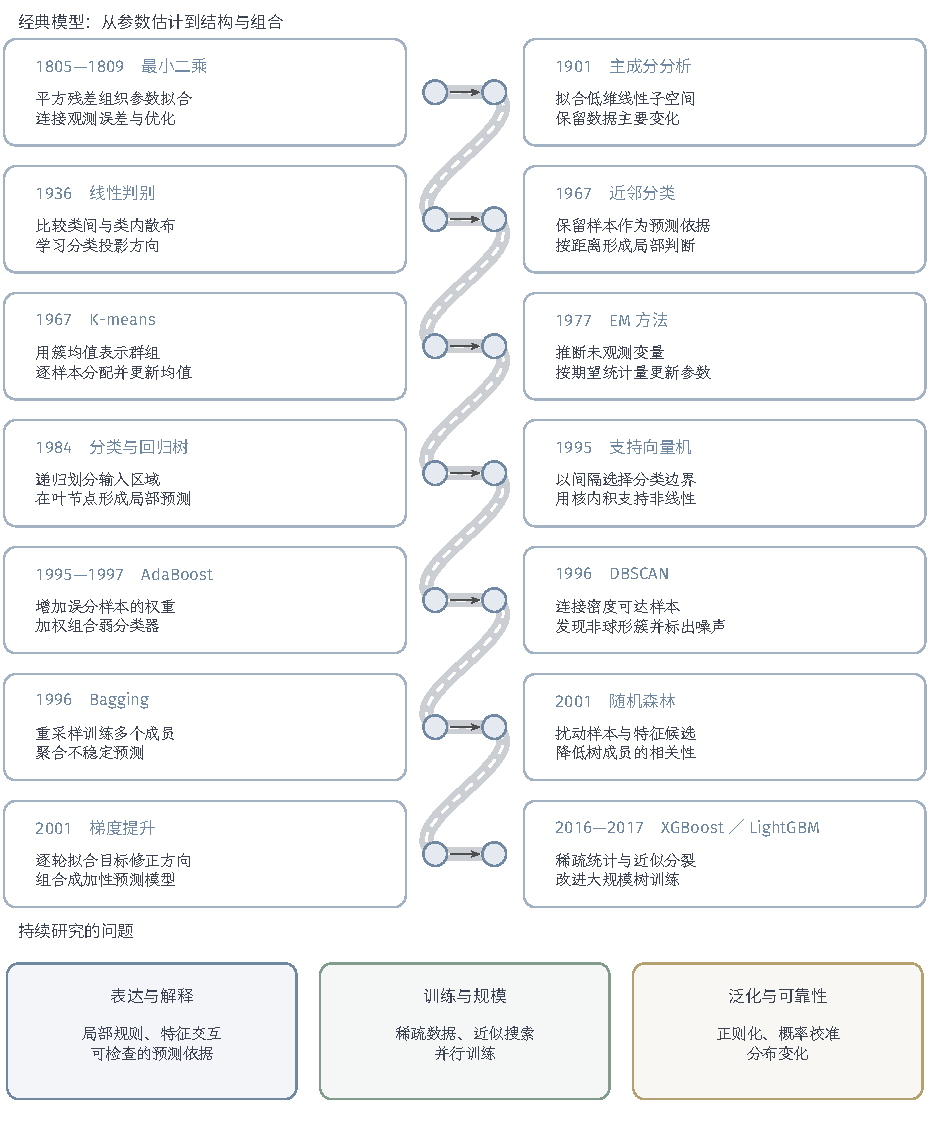
\includegraphics[width=157.406mm,height=.82\textheight,keepaspectratio]{figures/03-models/01-classic-models/tikz/classic-models-history/figure.pdf}
  \caption{经典模型的代表性发展节点。沿时间路径可观察参数估计怎样扩展到结构发现、局部预测、非线性表示和模型组合。节点间距不表示实际时间长度，年份对应代表工作；这些方法持续交叉使用，并非依次替代。底部列出仍需分别评价的表达、训练与预测问题。}
  \label{fig:classic-models-history}
\end{figure*}
\FloatBarrier

\section{经典模型的类型}
\label{sec:classic-overview-modeling}

以房屋数据为例，预测器可以假定面积等属性共同形成一个全局趋势，也可以主要参考相似房屋，或针对不同条件学习不同的局部规则。概率模型进一步说明相同输入下结果可能怎样变化，集成方法则组合多个成员的判断。这些思路允许交叉：一个模型可以同时使用线性关系和概率分布，也可以把树作为集成成员。下面沿着它们各自回答的问题，说明共享结构怎样随任务改变。

\subsection{基于线性关系的建模}
\label{sec:classic-overview-linear}

预测房价时，一个直接的起点是给面积、楼龄等特征分别赋予权重，再相加得到预测。设输入为$\bm{x}\in\mathbb{R}^{d}$，权重为$\bm{w}\in\mathbb{R}^{d}$，偏置为$b\in\mathbb{R}$，这个计算写成
\begin{equation}
  g(\bm{x})=\bm{w}^{\top}\bm{x}+b.
  \label{eq:classic-overview-linear-score}
\end{equation}
在线性回归中，$g(\bm{x})$可以直接作为价格预测；在二分类中，它可以作为类别得分，再按阈值给出类别。加权求和的结构相同，但回归系数需要贴合数值响应，分类权重需要帮助区分类别。得分也可以经适当转换得到类别概率，这就与后面的概率建模相接。

当目的从预测变成降维时，加权求和仍然有用，只是输出改为少数新的坐标。主成分分析（principal component analysis, PCA）选择若干投影方向，让保留的坐标描述数据的主要变化；这里学习方向的依据是输入自身的变化，而不是房价或类别标签。第\ref{sec:dim-pca}节会说明这一目标与重构误差的关系。同样的线性运算并不意味着相同的学习问题。

如果大户型和小户型的面积增量对应不同的价格变化，或面积的作用取决于楼龄，原始特征的加权和就可能过于受限。可以先加入面积平方、面积与楼龄的乘积等新特征，再学习它们的权重。这种\term{特征映射}（feature mapping）把原来的输入改写成另一组可供计算的特征，使简单的线性组合也能表达原始输入中的非线性关系。线性因而要相对于所用的特征来判断；第\ref{sec:regression-basis}节从基函数展开说明这种扩展。

平方项和交互项越多，显式保存的特征向量就越长。有些训练和预测过程只需要两份特征向量的内积，因而无需分别生成它们：只要有一个函数直接返回同样的内积，就能完成原来的计算。这类\term{核方法}（kernel method）通过内积函数指定特征空间，省去显式展开的成本。下面从一个圆形分类边界说明这种转换，再检查什么样的函数能够充当内积。

图\ref{fig:classification-kernel-map}用一个二维分类例子展示特征映射$\bm{\phi}(\bm{x})=(x_1,x_1^2+x_2^2)^{\top}$。输入空间中的圆$x_1^2+x_2^2=1$，在新坐标中变成直线$\phi_2=1$；同一得分$g(\bm{x})=1-x_1^2-x_2^2$于是可以写成$g(\bm{x})=(0,-1)\bm{\phi}(\bm{x})+1$。改变的是输入的表示，原来位于圆内与圆外的样本不需要改变类别。这幅图给定了一条可行边界，用于解释几何对应，不把它当作训练后的最大间隔解。

\begin{figure}[htbp]
  \centering
  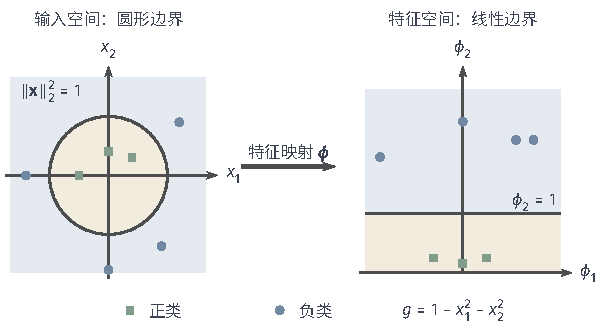
\includegraphics[width=103.166mm]{figures/03-models/01-classic-models/tikz/classification-kernel-map/figure.pdf}
  \caption{非线性边界在特征映射前后的对应，两个面板的坐标均无量纲。正类方点为$(-0.5,0)$、$(0,0.4)$、$(0.4,0.3)$，负类圆点为$(-1.4,0)$、$(0,-1.6)$、$(1.2,0.9)$、$(0.9,-1.2)$。右图逐点使用$\phi_1=x_1$、$\phi_2=x_1^2+x_2^2$；水平线$\phi_2=1$对应左图半径为1的圆。数据与边界均为教学构造。}
  \label{fig:classification-kernel-map}
\end{figure}

\subsubsection{特征映射与核技巧}
\label{sec:classic-overview-kernel-trick}
\label{sec:classification-svm-kernel-trick}

圆形边界的例子显式增加了一个平方特征；当特征更多时，逐一构造坐标可能成为计算负担。设特征映射$\bm\phi:\mathbb R^d\to\mathcal H$把输入送到带内积的特征空间，在那里使用线性预测器$f(\bm x)=\langle\bm w,\bm\phi(\bm x)\rangle+b$。若学习过程得到的权重可以写为$\bm w=\sum_{i=1}^n a_i\bm\phi(\bm x_i)$，代入预测式后，每个训练样本只通过一个特征内积参与计算：
\begin{equation}
  f(\bm x)=\sum_{i=1}^{n}a_iK(\bm x_i,\bm x)+b,
  \qquad K(\bm x,\bm z)=\langle\bm\phi(\bm x),\bm\phi(\bm z)\rangle_{\mathcal H}.
  \label{eq:classic-overview-kernel}
\end{equation}
这里$a_i$由具体学习目标确定，核$K$直接返回两份特征的内积。用核值替换特征内积的做法称为\term{核技巧}（kernel trick）。它不改变分类、回归或降维的目标，而是让这些目标在新的几何中计算；$K$对原输入可以非线性，预测也就能够具有非线性边界。只有计算可以写成这些内积时，才可直接作这种替换。

例如$K(\bm x,\bm z)=(\bm x^\top\bm z)^2$隐含平方项与交互项。训练时可以计算$n\times n$的核矩阵，再按具体目标求系数；预测时计算新输入与训练输入的核值，并按式\eqref{eq:classic-overview-kernel}加权。这省去了二次特征的显式展开，却将计算与存储转到了样本之间的关系上。无限维映射也可以用这种形式计算，其代价同样取决于需要访问多少训练样本（特征空间的背景参考\BookChapterRef{chap:functional-analysis-and-approximation}{第一卷“数学准备”的“函数空间”章}）。

\subsubsection{用正定核构造非线性特征空间}
\label{sec:classic-overview-kernel-validity}
\label{sec:classification-svm-mercer}

用函数$K$替代内积以后，还需要确认这个替代保持了内积的几何性质。特征向量线性组合的范数平方应当非负，因此对任意有限输入与实系数都必须有$\sum_{i,j}a_i a_jK(\bm x_i,\bm x_j)\geq0$；内积的对称性还要求$K$对称。这些条件使任意有限Gram矩阵半正定，也保证能在某个Hilbert空间中构造出相应特征内积。由此可以直接设计$K$，而不必先列出全部特征坐标（构造依据参考\BookTheoremRef{thm:functional-moore-aronszajn-construction}{第一卷“数学准备”的“正定核的RKHS构造”定理}）。

本书的“正定核”允许Gram矩阵奇异；需要排除互异输入下的退化时，才要求严格正定。半正定回答的是能否构造特征内积。核矩阵的可逆性、目标的求解难度和表示对任务的适合程度，则分别取决于数据、学习目标与核的选择。正则化和选解规则处理求解中的退化，核尺度等超参数通过独立验证选择。

非负加权和、核的乘积及逐点有限极限可以构造新核，分别对应特征直和、张量积及有限二次型极限。这些规则可以把多个信息来源组合成一个合法内积。某份训练集的矩阵通过检查，只认证这一组点；预测还会遇到新输入，因此核应在整个预期定义域上具有构造依据。在非空紧度量输入域上，若核连续，并使用有限、全支撑的Borel测度，可用Mercer展开得到显式谱坐标（参考\BookTheoremRef{thm:functional-mercer}{第一卷“数学准备”的“连续正定核的Mercer展开”定理}）。核技巧本身不要求先求出谱展开。

\subsubsection{常用核与表示选择}
\label{sec:classic-overview-common-kernels}
\label{sec:classification-svm-common-kernels}

回到$\bm{x},\bm{z}\in\mathbb{R}^d$。常用核之间的区别主要在于怎样度量接近程度、允许哪些特征交互，以及这些选择带来怎样的函数范数。表\ref{tab:classification-svm-kernels}列出五种常见形式，核尺度统一记为$\beta$，多项式次数记为$p$，避免与输入维数$d$混用。

\begin{table}[htbp]
  \centering
  \small
  \begin{tabularx}{\linewidth}{@{}>{\RaggedRight\arraybackslash}p{18mm}>{\RaggedRight\arraybackslash}X>{\RaggedRight\arraybackslash}p{27mm}@{}}
    \toprule
    名称 & $K(\bm{x},\bm{z})$ & 参数与正定性\\
    \midrule
    线性核 & $\bm{x}^{\top}\bm{z}$ & 半正定\\
    多项式核 & $(\beta\bm{x}^{\top}\bm{z}+r)^p$ & $\beta,r\ge0$，正整数$p$\\
    高斯RBF核 & $\exp(-\beta\lVert\bm{x}-\bm{z}\rVert_2^2)$ & $\beta>0$，半正定\\
    Laplacian核 & $\exp(-\beta\lVert\bm{x}-\bm{z}\rVert_1)$ & $\beta>0$，半正定\\
    Sigmoid形式 & $\tanh(\beta\bm{x}^{\top}\bm{z}+r)$ & 一般不保证半正定\\
    \bottomrule
  \end{tabularx}
  \caption{常用核函数与合法性条件。这里的“半正定”要求任意有限输入的Gram矩阵半正定；Sigmoid一行列出的是常见相似性形式，使用前仍需针对定义域与参数核验。}
  \label{tab:classification-svm-kernels}
\end{table}

\term{线性核}（linear kernel）对应$\bm{\phi}(\bm{x})=\bm{x}$，保留原始特征内积。对于线性预测，训练样本的核展开可以先聚合为一个权重向量，使用时只需与新输入作内积。是否加入非线性交互，取决于原特征中的线性组合能否描述目标规律；验证数据可以比较这两种表示在相同预测任务上的误差。输入维数只是表示的规模，本身没有回答哪种关系更适合任务。

\term{多项式核}（polynomial kernel）把有限阶交互隐式加入模型。以$d=2$、$\beta=1$、$r=0$、$p=2$为例，
\[
  \begin{aligned}
    (\bm{x}^{\top}\bm{z})^2
      &=x_1^2z_1^2+2x_1x_2z_1z_2+x_2^2z_2^2,\\
    \bm{\phi}(\bm{x})
      &=(x_1^2,\sqrt2\,x_1x_2,x_2^2)^{\top}.
  \end{aligned}
\]
交叉项前的$\sqrt2$使特征内积准确等于核值。一般地，令多重指标$\bm{a}=(a_1,\ldots,a_d)$满足$|\bm{a}|=\sum_j a_j=p$，并记$\bm{x}^{\bm{a}}=\prod_j x_j^{a_j}$、$\bm{a}!=\prod_j a_j!$。多项式展开为
\[
  (\bm{x}^{\top}\bm{z})^p
  =\sum_{|\bm{a}|=p}\frac{p!}{\bm{a}!}
     \bm{x}^{\bm{a}}\bm{z}^{\bm{a}}.
\]
所以齐次$p$次核可以使用$\binom{d+p-1}{p}$个单项式坐标；当$\beta>0,r>0$时，非齐次核包括$0$至$p$次项，一种完整单项式表示的维数是$\binom{d+p}{p}$。这些是特征数量，不是样本数量；计算一个核值通常只需一次$d$维内积和幂运算，节省的是显式特征展开成本，完整优化仍要另计。

\term{高斯径向基核}（Gaussian radial basis function kernel，Gaussian RBF kernel）根据欧氏距离赋予局部相似性。其无限维特征可以由指数级数直接看出：
\begin{equation}
  \begin{aligned}
    K(\bm{x},\bm{z})
      ={}&e^{-\beta\lVert\bm{x}\rVert_2^2}
          e^{-\beta\lVert\bm{z}\rVert_2^2}\\
       &\cdot\sum_{p=0}^{\infty}
          \frac{(2\beta)^p}{p!}
          (\bm{x}^{\top}\bm{z})^p.
  \end{aligned}
  \label{eq:classification-svm-rbf-expansion}
\end{equation}
每一阶多项式核都是半正定的，系数非负，两个单点因子可以吸收到特征中；级数逐点收敛，因而也给出了高斯核合法性的证明。把每一阶的单项式展开合并，坐标可写成
\[
  \phi_{\bm{a}}(\bm{x})
  =e^{-\beta\lVert\bm{x}\rVert_2^2}
     \sqrt{\frac{(2\beta)^{|\bm{a}|}}{\bm{a}!}}\,
     \bm{x}^{\bm{a}},
  \qquad \bm{a}\in\mathbb{N}_0^d.
\]
这里$\mathbb{N}_0$为非负整数集合，所有坐标平方之和等于$K(\bm{x},\bm{x})=1$。在整个$\mathbb{R}^d$上，这个核具有无限秩；限制到一批有限训练点以后，实际使用的Gram矩阵仍是$n\times n$。

参数$\beta$控制相似性随距离衰减的速度，也常写成$\beta=1/(2\sigma^2)$。较大$\beta$使不同训练点之间的相似性迅速减小，模型能够形成更局部的变化；较小$\beta$使作用范围更宽。对互异有限输入，高斯Gram矩阵严格正定，因此在不约束范数时，线性方程$\bm{K}\bm{a}=\bm{y}$允许核展开插值给定标签。然而所需系数与函数范数可能很大；固定范数、固定正则化强度或有重复输入且标签冲突时，都不能由“无限维”推出任意插值，更不能由插值推出泛化良好。

\term{Laplacian核}（Laplacian kernel）使用$L^1$距离，且可以分解成各坐标上的乘积：
\[
  \exp(-\beta\lVert\bm{x}-\bm{z}\rVert_1)
  =\prod_{j=1}^d\exp(-\beta|x_j-z_j|).
\]
一维形式的半正定性可由积分特征表示验证：
\[
  e^{-\beta|t|}
  =\int_{\mathbb{R}}e^{\mathrm{i}\omega t}
      \frac{\beta}{\pi(\beta^2+\omega^2)}\,\mathrm{d}\omega.
\]
其中$\mathrm{i}$为虚数单位。对任意有限个输入$x_j$和实系数$a_j$，将有限求和移入积分可得
\[
  \begin{aligned}
    &\sum_{j,k}a_j a_k e^{-\beta|x_j-x_k|}\\
    &\quad=\int_{\mathbb{R}}
      \left|\sum_j a_j e^{\mathrm{i}\omega x_j}\right|^2
      \frac{\beta}{\pi(\beta^2+\omega^2)}\,\mathrm{d}\omega
      \ge0.
  \end{aligned}
\]
多维形式再由核的乘积闭包得到。Laplacian核在零距离附近的变化方式与高斯核不同，可以作为直方图或稀疏特征上的另一种距离选择，但哪一种更适合仍取决于尺度、表示与验证结果。

常称为\term{Sigmoid核}（sigmoid kernel）的形式将内积送入双曲正切函数，形态上接近一个具有非线性激活的神经元，却不自动具有内积核的性质。甚至$\beta=1,r=0$也不能在整个实数域上保证半正定：对$x_1=1,x_2=2$，二阶Gram行列式为
\[
  \tanh(1)\tanh(4)-\tanh(2)^2
  \approx-0.1683<0.
\]
因此“参数取正”并不足以保证合法。某个有限数据集上矩阵没有负特征值，只说明当前矩阵通过检查；若要保留依赖内积核的几何与优化解释，应选用在目标定义域上已确认半正定的核。

对字符串、图与树，核技巧同样适用。\term{字符串核}（string kernel）可以计数共同的子串或子序列，\term{图核}（graph kernel）可以比较局部子结构，\term{树核}（tree kernel）可以比较子树模式。若将每种模式的出现次数作为一个坐标，两对象的模式计数内积就给出了直接的正定构造；动态规划或结构化计数有时能避免把全部坐标显式列出。这样的\term{结构化核}（structured kernel）把输入的组合结构用于相似性计算，适用于序列分析、分子图或句法树等场景，并通过可验证的特征内积保留核方法的几何与优化性质。

\subsubsection{核矩阵的使用与中心化}
\label{sec:classic-overview-kernel-matrix}

用训练样本进行核计算，需要组织样本两两之间的内积。核矩阵的元素为$\bm{K}_{i,j}=K(\bm{x}_i,\bm{x}_j)$，在$n$个训练输入上完整保存它需要$O(n^2)$空间和$O(n^2)$次核计算。省去显式特征以后，样本数便成为这一实现的主要规模变量。缓存、稀疏化或低秩近似可以改变计算成本；采用近似时，还要检查被省去的关系对当前任务有多大影响。

有些方法要求在特征空间中先减去训练均值。令$\bm{1}\in\mathbb{R}^{n}$为全一向量、$\bm{I}_n$为单位矩阵，中心化矩阵及中心化核矩阵为
\begin{equation}
  \bm{H}=\bm{I}_n-\frac1n\bm{1}\bm{1}^{\top},
  \qquad \bm{K}_{\mathrm{c}}=\bm{H}\bm{K}\bm{H}.
  \label{eq:classic-overview-kernel-centering}
\end{equation}
左乘$\bm{H}$减去各列均值，右乘$\bm{H}$减去各行均值；展开双边乘积时，还要加回原核矩阵的整体均值。所得矩阵等于中心化特征的内积矩阵。非线性映射与减均值的操作一般不能交换，因此所需的是特征空间中的训练均值，新样本也使用这个固定的中心。是否执行这一步由学习目标决定：核PCA考察围绕特征均值的变化，需要中心化；高斯过程则按选定的均值函数与协方差模型处理数据。


核支持向量分类器在特征空间中学习分界，核支持向量回归拟合数值响应，核PCA保留特征空间方差，核K-means则优化特征空间的簇内距离。四者共享核定义的几何，但学习目标不同；相应入口见第\ref{sec:classification-svm-kernels}、第\ref{sec:regression-kernel-svr}、第\ref{sec:dim-kpca}和第\ref{sec:clustering-partition}节。非线性表达来自映射，映射是否适合任务仍需结合数据判断。

\subsection{基于邻域的建模}
\label{sec:classic-overview-neighborhood}

另一种做法是直接寻找与待预测房屋相似的成交记录。\term{邻域}（neighborhood）指按选定距离或相似关系找到的一组附近样本；模型主要利用这些样本的信息，而不必为所有房屋规定同一个全局趋势。$k$近邻（$k$-nearest neighbors, $k$-NN）用最近的$k$个样本构成邻域：回归时可以平均它们的价格，分类时可以让它们的类别投票，也可以给更近的样本更大权重。改变的是聚合的对象和产生输出的规则，寻找邻居的计算则可以复用。

没有响应或类别时，邻域还可以提供样本之间的结构证据。密度聚类考察一个位置附近是否有足够多的样本，再按相应规则连接稠密区域；基于图的方法把样本作为节点，把选定的相似关系作为边。图结构可以用于寻找群组，也可以在少量样本有标签时约束标签传播。用于降维时，则可以要求原本相近的样本在低维表示中仍保持邻近。距离、邻域和图因此连接了预测、聚类与表示学习，但“同一簇”“同一类别”和“相近坐标”仍是不同的要求。

保留全部邻居库会增加存储和查询成本，一种简化是用少量\term{原型}（prototype）概括样本群体，再比较查询点与这些代表的距离。最近质心分类器用每个已知类别的中心作代表；K-means在没有类别标签时，同时寻找中心和样本分组。二者都比较样本与代表，但只有前者事先知道类别，原型也未必是查询点附近的真实样本。第\ref{sec:classification-instances-comparison}节与第\ref{sec:clustering-partition}节分别讨论这两种使用方式。

这些做法都依赖“相近”的含义。\term{相异度}（dissimilarity）用较小值表示更相近，不一定满足距离度量的全部条件；需要三角不等式的计算不能直接用于任意相异度。房屋在面积上接近，却可能位于不同地区；把面积、楼龄和位置直接混在一个距离中，也可能让数值尺度较大的属性主导邻居选择。表示和度量决定邻域，邻域再影响预测、连通与布局。第\ref{sec:regression-instance}节和第\ref{sec:classification-instances}节比较局部预测，第\ref{sec:clustering-density}节与第\ref{sec:clustering-graph}节讨论群组结构，第\ref{sec:dim-neighbors}节讨论低维布局应保留哪些邻域关系。

\subsection{基于树与规则的建模}
\label{sec:classic-overview-tree-rules}

如果不同房屋适合采用不同的预测规则，可以通过具体条件划分输入。例如，对某个地区的房屋按面积划分，再对其中一组按楼龄划分。\term{决策树}（decision tree）把这些条件组织成逐层分支的结构：输入沿分支到达一个叶节点，再使用该叶的预测。每条路径规定一个区域，不同区域可以采用不同的局部判断。

回归树和分类树共享这套划分结构。采用平方损失时，常数叶的回归树在叶内给出响应均值；分类树可以给出类别或类别比例。因为要拟合的目标不同，选择分裂的准则也随之改变。回归还可以在叶内拟合线性模型，使一片区域既有条件边界，也有局部趋势。这里同时用到了分区和线性关系，说明建模思路可以组合。第\ref{sec:regression-trees}节与第\ref{sec:classification-trees}节分别展开这些训练与预测过程。

树路径也可以写成“如果若干条件成立，就给出某个结论”。\term{规则模型}（rule-based model）直接学习和组织这类条件，规则之间可以重叠，也可能有优先顺序，不必形成一棵完整的树。第\ref{sec:classification-rules}节会说明怎样处理覆盖、冲突和默认类别。浅树或短规则便于检查具体条件，但随着分支或规则数量增加，理解整个决策过程也会变得困难；只凭表示形式不能认定一个模型已经容易解释。

树还可以组织嵌套群组。层次聚类逐步合并或分裂样本组，保留不同粒度下的包含关系；其树描述分组层次，决策树的分支则描述输入条件与预测路径。二者都使用树形结构，但学习准则与输出不同，不能直接共用分类树的分裂规则，详见第\ref{sec:clustering-hierarchy}节。

\subsection{基于概率的建模}
\label{sec:classic-overview-probabilistic}

同样面积、楼龄和位置的房屋，成交价格仍会变化。只输出一个数值，会省去这种变化的描述。\term{概率建模}（probabilistic modeling）为相关变量建立概率分布，用分布说明哪些结果更可能出现，以及结果可能怎样分散。回归可以描述给定输入后的响应分布，也可以对未知系数或函数设置先验，再根据观测形成后验。响应本身的变化与有限数据造成的估计不确定性由此有了不同的建模位置；第\ref{sec:regression-probabilistic}节进一步说明这一差别。

分类关注的则是给定输入后的类别概率。可以直接建立这一条件分布，也可以先描述各类别内部的输入分布及类别出现的比例，再通过贝叶斯公式计算类别概率。前一种思路通向Logistic回归等条件模型，后一种思路通向朴素贝叶斯等生成式分类器。朴素贝叶斯用“给定类别后各特征条件独立”的假设简化联合分布，这个假设不等于说所有房屋属性在总体中互不相关。第\ref{sec:classification-probability}节比较这些分布设定怎样改变训练与决策。

若类别没有给出，可以把群组归属作为\term{潜变量}（latent variable），即参与解释观测、却没有直接记录在数据中的随机量。高斯混合模型（Gaussian mixture model, GMM）用多个成分分布共同描述输入，并估计一个样本属于各成分的概率；聚类结果的含义依赖这些成分是否适合所要寻找的群组。降维中的潜变量承担另一种职责：它是少量潜在坐标，模型用这些坐标及噪声生成高维观测。概率主成分分析把这一生成关系设为线性，高斯过程潜变量模型则允许非线性映射。第\ref{sec:clustering-gmm}节与第\ref{sec:dim-probabilistic}节会分别说明离散群组和低维坐标的作用。

概率模型还需要具体的函数或相似关系来连接输入与结果，因此可以与前面的表示结合。贝叶斯线性回归仍使用线性函数，高斯过程用核描述不同输入处函数值的协方差，潜变量模型则用线性或非线性映射描述观测怎样产生。计算得到的概率是在这些假设下成立的模型输出。拟合与校准方法固定后，还需用独立样本比较报告概率与事件频率，检验模型输出的样本外校准（参考\BookSectionRef{sec:reliability-output-evaluation}{第二卷“基础、理论和可信性”的“可靠性”章“概率与预测范围的检验”小节}）。

\subsection{基于集成的建模}
\label{sec:classic-overview-ensemble}

同一个预测任务可以训练出不同模型。一棵树可能对训练样本的少量变化很敏感，一个简单线性模型也可能留下系统性的预测误差。\term{集成学习}（ensemble learning）通过训练多个成员并组合它们的输出，改变整体模型的预测方式。成员通常称为\term{基学习器}（base learner）；组合能否带来收益，既取决于成员各自的表现，也取决于它们是否反复犯相同的错误。

为减弱训练样本扰动造成的预测波动，可以从原训练集有放回地抽取多份数据，通常每份包含与原集相同数量的样本。分别训练成员后，回归采用预测平均，分类采用投票汇总。这种\term{装袋法}（bootstrap aggregating, Bagging）用重采样产生不同成员，再通过聚合抵消一部分波动。随机森林还在节点分裂时随机选择候选特征，使各棵树有机会形成不同划分。成员若仍反复犯相同的错误，聚合的收益就会受到限制\scite{breiman1996bagging,breiman2001randomforests}。第\ref{sec:ensemble-bagging}节进一步说明自助样本、袋外预测和树成员随机化。

针对尚未拟合好的部分，可以让新成员接着已有预测训练。\term{Boosting}（提升）逐轮加入成员，使后续学习回应当前整体模型的不足。AdaBoost依据当前分类错误重新加权样本，让分错的样本在下一轮更受重视；梯度提升则根据所选损失确定每一轮应拟合的修正方向，平方损失回归中的修正可以直接表现为当前残差。任务与损失改变后，修正的含义也会改变，所以“每轮拟合残差”不能概括所有Boosting方法。

提升的可学习性保证针对可实现的二分类任务，使用独立同分布抽样、预先固定且VC维有限的基类，并满足相应可测条件。若同一弱学习器在所有允许的可实现分布上，包括提升过程产生的重加权分布，都能按指定成功概率取得统一的正优势，就可以选择足够轮数和样本量，将总体零一风险控制到任意预设精度（参考\BookSectionRef{sec:boosting}{第二卷“基础、理论和可信性”的“二分类学习的可学习性”章“集成学习”节}）。前向逐步建模和现代梯度提升树见第\ref{sec:ensemble-boosting}节\scite{friedman2001gradientboost}。

线性模型、近邻和树可能利用了不同的预测信息，此时组合方式也可以由数据学习。\term{Stacking}（堆叠）把成员预测作为另一层模型的输入，由\term{元学习器}（meta-learner）学习怎样组合这些预测。用于训练组合层的预测应来自没有用对应样本拟合的成员，例如交叉验证中的折外预测；否则，组合层看到的误差可能小于部署时的误差。混合不同类型的成员增加了可用的组合，但训练需要多层数据安排，预测也要运行多个模型。完整流程见第\ref{sec:ensemble-stacking}节\scite{wolpert1992stacked}。

\Needspace{18\baselineskip}
\section{本章小结}
\label{sec:classic-overview-summary}

房屋成交数据说明了任务与模型表示的分工。任务规定要得到价格、类别、群组或低维坐标，表示则规定怎样利用特征和样本得到这些结果。加权和既可以输出价格，也可以输出类别得分或投影坐标；邻域中的同一批记录既可以提供响应均值，也可以提供类别投票。换任务后，计算结构可能保留，评价预测和选择模型的准则却必须相应改变。

同一个模型还可以组合几种思路。特征映射与核扩展线性表示，输入分区中的叶节点可以使用局部线性模型，概率分布可以描述这些预测中的不确定性，多个成员又可以进一步集成。后续章节把这些组合放回具体任务，说明要估计什么、怎样求解，以及用什么新样本证据评价。第\ref{chap:regression}章从数值响应开始，使输出目标与表示方式的区别成为一个可计算的问题。

\paragraph{扩展阅读}
Hastie、Tibshirani与Friedman的《统计学习基础》在共同的预测框架中比较线性、核、邻域、树和集成，适合进一步考察表示与学习准则怎样共同决定方法。Bishop的教材从概率模型展开这些联系，并说明潜变量怎样参与解释未标注观测\scite{hastie2009,bishop2006}。

\chapter{回归}
\label{chap:regression}

预测房屋价格时，可以估计平均成交价，也可以给出预算所需的上分位数或价格分布。\term{回归}（regression）根据输入估计数值响应的这些条件特征。设训练集为$D_n=\{(\bm{x}_i,y_i)\}_{i=1}^{n}$，其中$\bm{x}_i\in\mathbb{R}^{d}$为输入，$y_i\in\mathbb{R}$为响应，预测函数记为$f$；响应也可以是次数等离散数值。

回归的计算起点可追溯到19世纪初的最小二乘法，“回归”这一名称则来自Galton在1886年对亲子身高的研究。1970年代的广义线性模型扩展了响应类型，1980年代的回归树表达条件分区，1990年代的支持向量回归及随后发展的树集成进一步容纳非线性与交互\scite{galton1886,nelder1972glm,breiman1984cart}。

如今，需要检查变量作用或建立简洁基线时，线性模型仍是常见起点；面对复杂表格数据，随机森林与梯度提升树是常用候选。现代基准中，梯度提升树在多类表格任务上仍有竞争力；具体比较同时受到数据、调参与计算预算的影响\scite{erickson2026tabarena}。

预测对象确定以后，还要选择输入与响应之间的关系。全局加权适合描述共同趋势，邻域方法在查询点附近估计响应，树与规则为不同条件分配局部预测；概率模型保留分布信息，集成则组合多个成员。各节沿着这些关系展开训练目标与求解过程，再考察新输入上的预测误差。第\ref{chap:classic-models-overview}章建立的建模思路，在这里由数值响应及其损失具体化。

\section{基于线性关系的回归}
\label{sec:regression-linear}

预测房价的一个起点是给输入特征赋予权重，用加权和表示整体趋势。要由数据选出权重，就需要规定什么误差值得减小，以及多大的系数变化可以接受。最小二乘用平方残差评价拟合，正则化限制系数，分位数回归和SVR则改变误差的计分方式。原特征的线性关系不足时，还可以增加基函数或采用核；响应的取值范围与分布特征，则由GLM和GAM进一步处理。

\subsection{普通最小二乘（OLS）}
\label{sec:regression-ols}

从样本中选择一组系数，需要先规定怎样衡量预测误差。\term{普通最小二乘}（ordinary least squares, OLS）选择使残差平方和最小的系数。它既可以作为一个无需指定响应分布的优化准则，也可以在高斯噪声模型下解释为最大似然估计；以下先建立前一种形式，再说明统计结论需要哪些额外条件\scite{bishop2006}。

这种误差准则早于“回归”的名称。Legendre在1805年公开发表最小二乘法时，面对的是观测方程多于未知量、各方程通常无法同时精确成立的问题；误差平方和提供了在不一致观测之间取舍的准则。Gauss在1809年的天体轨道著作中又从观测误差的概率分析出发讨论其依据\scite{stigler1981,gauss1809}。

\subsubsection{模型结构}
\label{sec:regression-ols-structure}

令$\bm{\phi}(\bm{x})\in\mathbb{R}^{p}$表示固定特征向量，模型写成$f_{\bm{w}}(\bm{x})=\bm{\phi}(\bm{x})^{\top}\bm{w}$，其中$\bm{w}\in\mathbb{R}^{p}$。最简单的选择是$\bm{\phi}(\bm{x})=(1,\bm{x}^{\top})^{\top}$，此时$p=d+1$，第一个系数为截距。这里的“线性”指预测对待估计系数线性；特征变换$\bm{\phi}$可以非线性，其具体形式将在本小节后面展开。

把样本堆叠为设计矩阵$\bm{X}\in\mathbb{R}^{n\times p}$，第$i$行为$\bm{\phi}(\bm{x}_i)^{\top}$，并记$\bm{y}=(y_1,\ldots,y_n)^{\top}$，得到目标
\begin{equation}
  \widehat{\bm{w}}\in\argmin_{\bm{w}}J(\bm{w}),
  \qquad
  J(\bm{w})=\frac{1}{2n}\lVert\bm{y}-\bm{X}\bm{w}\rVert_2^2.
  \label{eq:regression-ols-objective}
\end{equation}
因子$1/(2n)$不改变OLS的最优解，但会影响梯度、步长和正则系数的数值约定。本章使用平均平方损失时均沿用这一形式。

图\ref{fig:regression-ols-residuals}把这个目标放回输入与响应平面：每条虚线都是固定$x_i$之后，观测$y_i$与直线预测之间的纵向差。OLS选择的是让这些差的平方和最小的直线，因此拟合线通常不穿过每个样本；图中的距离沿响应轴测量，区别于点到直线的垂直几何距离。

\begin{figure}[htbp]
  \centering
  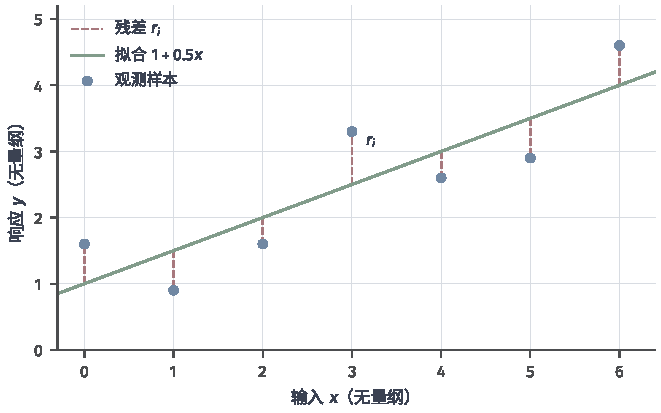
\includegraphics[width=105.412mm]{figures/03-models/01-classic-models/matplotlib/regression-ols-residuals/figure.pdf}
  \caption{一维OLS与响应残差。七个构造样本的最小二乘直线为$\widehat f(x)=1+0.5x$；蓝色实心点表示观测，绿色实线表示预测，红色竖虚线表示$r_i=y_i-\widehat f(x_i)$。横、纵轴均为无量纲教学变量。}
  \label{fig:regression-ols-residuals}
\end{figure}

响应二阶矩有限时，条件均值在平方可积预测函数中达到最小风险，且只在输入分布的几乎处处意义下唯一（参考\BookTheoremRef{thm:probability-conditional-mean-l2-projection}{第一卷“数学准备”的“条件均值的平方损失最优性”定理}）。
限制为$f_{\bm w}$以后，若条件均值不属于所选模型类，OLS估计的只是该类中的平方逼近；
高斯性、同方差性与误差对称性都不是平方损失以条件均值为目标的必要条件。

\subsubsection{参数学习}
\label{sec:regression-ols-learning}

目标的梯度为$\bm{X}^{\top}(\bm{X}\bm{w}-\bm{y})/n$，Hessian为$\bm{X}^{\top}\bm{X}/n$，后者半正定。因此使梯度为零既是必要条件，也是充分条件，得到\term{正规方程}（normal equations）：残差与每一列特征都正交。
\begin{equation}
  \bm{X}^{\top}\bm{X}\widehat{\bm{w}}=\bm{X}^{\top}\bm{y}.
  \label{eq:regression-normal-equations}
\end{equation}

正规方程的全部参数解为$\bm X^\dagger\bm y+\operatorname{null}(\bm X)$（参考\BookTheoremRef{thm:matrix-analysis-pseudoinverse-minimum-norm}{第一卷“数学准备”的“最小二乘与最小范数”定理}）。
因此训练拟合值总是唯一，参数唯一则要求设计矩阵列满秩；否则可取最小范数解。
零空间中的参数差在训练点上不可见，却可能在新特征向量上产生不同预测。

闭式表达用于分析，计算时通常不显式求逆。列满秩且$n\geq p$时，薄QR分解$\bm{X}=\bm{Q}\bm{R}$把问题化为三角方程$\bm{R}\widehat{\bm{w}}=\bm{Q}^{\top}\bm{y}$，稠密计算代价约为$O(np^2)$。秩亏或需要检查小奇异值时可以用SVD。直接形成$\bm{X}^{\top}\bm{X}$会把满列秩矩阵的二范数条件数平方，因此近似共线时尤其应避免求逆实现。

当矩阵分解不便进行时，可迭代更新
\begin{equation}
  \bm{w}^{(t+1)}
  =\bm{w}^{(t)}+\frac{\eta}{n}
       \bm{X}^{\top}(\bm{y}-\bm{X}\bm{w}^{(t)}).
  \label{eq:regression-ols-gradient}
\end{equation}
一次完整更新需要$O(np)$次算术操作；使用大小为$b$的小批量时，一次梯度估计需$O(bp)$，但总更新次数和随机误差也须考虑。代码\ref{code:regression-ols}展示矩阵求解接口与预测；截距列需由调用者加入，返回的秩可用于检查参数是否可识别。

\begin{codeblock}[language=Python,label={code:regression-ols},unbreakable]{用最小二乘接口求解并预测}
import numpy as np

# X: (n, p), y: (n,), X_new: (n_new, p)
# 截距列与特征变换在训练、预测时保持一致。
w, residuals, rank, singular_values = np.linalg.lstsq(
    X, y, rcond=None
)
y_pred = X_new @ w
\end{codeblock}

\subsubsection{理论分析}
\label{sec:regression-ols-theory}

解正规方程得到的是当前数据上的最小平方误差，未来预测还取决于数据怎样产生。我们先检查固定特征能表达哪些函数、梯度迭代怎样选解，再在固定设计下量化参数误差对新输入的影响。把输入也作为随机样本时，分析对象才转为估计量的渐近分布；相应假设需要随这一转换改变。

\paragraph{表达能力}
固定特征决定了OLS的候选函数：每个候选都是这些特征的线性组合。加入平方项或其他基函数可以表示原输入上的弯曲关系，但有限基只能覆盖其张成空间。即使精确求得最优系数，张成空间之外的目标变化仍会留下逼近误差。

\paragraph{收敛性}
令$\bm A=\bm X^\top\bm X/n$。当$\bm X\ne\bm0$且
$0<\eta<2/\lambda_{\max}(\bm A)$时，式\eqref{eq:regression-ols-gradient}的迭代在非零谱方向收敛；秩亏时零空间分量保持初值，
从零启动得到最小范数解（参考\BookTheoremRef{thm:gradient-descent-minimum-norm}{第一卷“数学准备”的“最小二乘梯度迭代的解选择”定理}）。该结论适用于这里固定训练目标的完整梯度迭代；新样本风险还需要下面的统计分析。
学习率应按当前平均损失的谱尺度选取。

\paragraph{泛化性}
求到经验最优解后，还需考察有限样本造成的估计误差及其对新输入预测的影响。偏差与方差分析需要指定响应如何产生。以下条件于固定设计，假设
\begin{equation}
  \bm{y}=\bm{X}\bm{w}_{\star}+\bm{\varepsilon},\qquad
  \mathbb{E}[\bm{\varepsilon}\mid\bm{X}]=\bm{0},\qquad
  \operatorname{Cov}(\bm{\varepsilon}\mid\bm{X})=\sigma^2\bm{I}_n,
  \quad 0<\sigma^2<\infty.
  \label{eq:regression-gauss-markov-model}
\end{equation}
这些条件要求均值模型正确、误差同方差且两两不相关；不相关不等于独立，也没有要求高斯分布。

\Needspace{9\baselineskip}
若设计矩阵列满秩，OLS无偏，协方差为$\sigma^2(\bm X^\top\bm X)^{-1}$；在条件于设计固定、对所有真参数均无偏的线性估计中，它具有最小协方差（参考\BookTheoremRef{thm:statistics-gauss-markov}{第一卷“数学准备”的Gauss--Markov定理}）。本节进一步说明该协方差怎样影响新输入的回归预测。

Gauss--Markov定理比较的是线性无偏估计量的协方差。要将这一结论用于预测，固定一个新特征向量$\bm{\phi}_{\star}$，估计其条件均值的均方误差为$\sigma^2\bm{\phi}_{\star}^{\top}(\bm{X}^{\top}\bm{X})^{-1}\bm{\phi}_{\star}$；预测带独立同方差噪声的未来响应时，再加上$\sigma^2$。新输入在设计的小特征值方向上分量较大时，逆矩阵会放大相应的估计误差，这也解释了远离训练范围的预测为何可能不稳定。

异方差不会在零条件均值下破坏OLS无偏性，但会改变协方差。若已知正定误差协方差$\bm{\Omega}$，最小化$(\bm{y}-\bm{X}\bm{w})^{\top}\bm{\Omega}^{-1}(\bm{y}-\bm{X}\bm{w})$得到\term{广义最小二乘}（generalized least squares, GLS），即按噪声结构重新度量残差；对角$\bm{\Omega}$对应加权最小二乘。用$\bm{\Omega}^{-1/2}$变换数据即可回到同方差问题。若协方差也需估计，须另行考虑其误差。

固定维数下的一致性可以直接由协方差得到。若固定设计序列满足$\bm{X}^{\top}\bm{X}/n\to\bm{Q}\succ0$，并在每个$n$下满足式\eqref{eq:regression-gauss-markov-model}，则
\[
  \mathbb{E}[\lVert\widehat{\bm{w}}-\bm{w}_{\star}\rVert_2^2\mid\bm{X}]
  =\frac{\sigma^2}{n}\operatorname{tr}
       \bigl((\bm{X}^{\top}\bm{X}/n)^{-1}\bigr)\longrightarrow0.
\]
均方一致性进而给出依概率一致性。渐近正态性还需要中心极限定理的条件。例如，设样本对$(\bm{z}_i,\varepsilon_i)$独立同分布，其中$\bm{z}_i=\bm{\phi}(\bm{x}_i)$。若其共同分布满足$\mathbb{E}\lVert\bm{z}\rVert_2^2<\infty$、$\bm{Q}=\mathbb{E}[\bm{z}\bm{z}^{\top}]\succ0$，且$\mathbb{E}[\varepsilon\mid\bm{z}]=0$、$\mathbb{E}[\varepsilon^2\mid\bm{z}]=\sigma^2<\infty$，则
\[
  \sqrt n(\widehat{\bm{w}}-\bm{w}_{\star})
  =
  (\bm{X}^{\top}\bm{X}/n)^{-1}
  \frac{1}{\sqrt n}\sum_i\bm{z}_i\varepsilon_i
  \ \xrightarrow{d}\ \mathcal{N}(\bm{0},\sigma^2\bm{Q}^{-1}).
\]
这里分别对Gram矩阵使用大数定律、对独立的$\bm{z}_i\varepsilon_i$使用多元中心极限定理，再用Slutsky定理合并。仅有误差不相关并不足以直接调用该中心极限定理。若误差条件高斯，OLS在有限样本下已经具有相应高斯分布，并与高斯似然的最大似然估计一致。

\subsubsection{支持非线性映射（多项式回归与基函数展开）}
\label{sec:regression-basis}

价格随面积变化未必是一条直线，但仍可使用线性参数模型。选择$\bm{\phi}(\bm{x})$后，所有正规方程与求解方法都保持不变，改变的是设计矩阵各列的含义。例如一维多项式使用$1,x,\ldots,x^q$，径向基使用$\exp(-(x-c_j)^2/(2s^2))$，其中中心$c_j$和尺度$s>0$预先给定或在训练过程中选择。

样条用分段多项式描述局部变化，并约束分段之间如何连接。带结点$\xi_1,\ldots,\xi_K$的三次样条可用$1,x,x^2,x^3$及$(x-\xi_k)_+^3$展开，其中$(a)_+=\max(a,0)$；只保留截断三次项会遗漏全局多项式部分。基函数越多，表达越灵活，也越可能出现高方差与病态设计。核方法将显式基的内积计算换为核值计算；采用固定核时，其特征表示也随之给定\scite{hastie2009}。

\subsubsection{支持异常值鲁棒性（Huber回归与M估计）}
\label{sec:regression-huber}

平方损失把十倍残差变成一百倍损失，少量错误记录因此可能主导拟合。\term{Huber损失}（Huber loss）在小残差处保持二次形状，在大残差处改为线性增长，从而限制残差方向的导数。它来自稳健位置估计的研究，也可用于回归目标\scite{huber1964}。
\begin{equation}
  \rho_\delta(r)=
  \begin{cases}
    r^2/2,&|r|\leq\delta,\\
    \delta|r|-\delta^2/2,&|r|>\delta,
  \end{cases}
  \qquad\delta>0.
  \label{eq:regression-huber-loss}
\end{equation}
对$r_i=y_i-\bm{\phi}(\bm{x}_i)^{\top}\bm{w}$最小化$\sum_i\rho_\delta(r_i)$，估计方程为$\sum_i\bm{\phi}(\bm{x}_i)\psi_\delta(r_i)=\bm{0}$，其中$\psi_\delta(r)=\max(-\delta,\min(r,\delta))$。令$a_i=\min(1,\delta/|r_i|)$，在$r_i=0$时取$a_i=1$，便可交替计算残差权重与加权最小二乘；应检查目标和估计方程的收敛。阈值$\delta$具有响应单位，常结合稳健尺度估计选择；采用中位绝对偏差定标时，还需按误差分布校准所用倍数。

将一般残差函数$\rho$代入$\min_{\bm{w}}\sum_i\rho(r_i)$，便得到以回归参数为目标的\(M\)估计（参考\BookSectionRef{sec:statistics-likelihood-robustness}{第一卷“数学准备”的“有限维目标的估计”小节}）。Huber准则凸且连续可微；Tukey双权、Cauchy等准则则可能非凸，求解与统计性质须分别分析。估计方程中的样本贡献是特征向量与$\psi_\delta$的乘积。有界残差导数限制了响应方向的影响，但远离其他输入的高杠杆点仍可因特征幅度较大而主导估计。Huber准则拟合的是自身损失下的最优中心；条件分布偏斜时，该中心可能偏离条件均值。

\subsubsection{小结}

OLS把预测误差化为特征列空间中的投影问题。列满秩时参数唯一；秩亏时训练拟合值仍唯一，而不同参数解可能在新输入上给出不同预测。无偏性、最小协方差和渐近分布则分别依赖均值模型、误差协方差和抽样条件。接下来改变的是两个不同环节：正则化控制数据难以确定的系数方向，其他损失则重新规定要拟合的响应中心。

\subsection{正则化线性回归}
\label{sec:regression-regularization}

面积与套内面积高度相关时，许多系数组合能产生近似相同的训练预测，数据却难以分辨它们。\term{正则化}（regularization）在拟合准则中加入参数约束或惩罚，限制这些缺少数据支持的变化。它可以降低估计方差，也会引入偏差；是否改善未来预测取决于真实结构、正则强度和测试分布。

\subsubsection{模型结构}
\label{sec:regression-penalties}

本小节将截距$b$与斜率$\bm{w}\in\mathbb{R}^d$分开。平方损失下，固定斜率的最优截距为$b=\bar y-\bar{\bm{x}}^{\top}\bm{w}$，所以可先用训练均值中心化特征与响应，只优化斜率，再恢复截距。以下$\bm{X},\bm{y}$均指中心化后的量，截距不受惩罚；需要标准化时，尺度也只能从训练集估计。

四种常见方法都在$\lVert\bm{y}-\bm{X}\bm{w}\rVert_2^2/(2n)$之外增加凸惩罚。\term{岭回归}（ridge regression）使用$\lambda\lVert\bm{w}\rVert_2^2/2$抑制参数幅度，收缩数据约束较弱的方向。Hoerl与Kennard在1970年的论文中系统研究了非正交设计下的有偏估计：当共线性使OLS方差过大时，容许一定偏差可能换来较小的均方误差\scite{hoerl1970ridge}。

\term{Lasso}（least absolute shrinkage and selection operator）使用$\lambda\lVert\bm{w}\rVert_1$。绝对值惩罚在零点有尖点，使部分坐标即使受到损失项的非零斜率推动，也仍可在零点取得最优值；下面会用左右导数说明这一点。Tibshirani在1996年提出这一方法，将连续收缩与变量选择放进同一个优化问题；与岭的差别因而不只是惩罚曲线的形状，还在于能否直接得到零系数\scite{tibshirani1996lasso}。

\term{弹性网}（elastic net）使用$\lambda_1\lVert\bm{w}\rVert_1+\lambda_2\lVert\bm{w}\rVert_2^2/2$，结合坐标稀疏与二次收缩；常写作$\lambda_1=\lambda\alpha$、$\lambda_2=\lambda(1-\alpha)$，其中$0\leq\alpha\leq1$。Zou与Hastie在2005年研究了这种结合，以改善高相关特征下的选择与估计。这里采用直接混合惩罚的形式；原始文献还讨论了对系数重标定以修正过度收缩的版本\scite{zou2005elastic}。

\term{组Lasso}（group Lasso）使用$\lambda\sum_{g=1}^{G}\omega_g\lVert\bm{w}_{A_g}\rVert_2$，其中$A_1,\ldots,A_G$是不重叠的坐标组，$\omega_g>0$为组权重，常取$\sqrt{|A_g|}$。Yuan与Lin在2006年将选择单位扩展到成组变量，例如一个分类特征展开的多个指示变量。该惩罚允许一整组变成零向量；被保留组中的各个坐标不必都非零\scite{yuan2006group}。

表\ref{tab:regression-regularization-comparison}将四种方法放在相同的平方损失下比较。选择方法时，需要区分“系数整体变小”“某个坐标变零”和“某组变量一起变零”；这三种要求对应不同的结构假设。

\begin{table*}[t]
  \centering
  \small
  \setlength{\tabcolsep}{4pt}
  \renewcommand{\arraystretch}{1.25}
  \begin{tabularx}{\linewidth}{@{}>{\RaggedRight\arraybackslash}p{16mm}>{\RaggedRight\arraybackslash}p{42mm}>{\RaggedRight\arraybackslash}p{24mm}>{\RaggedRight\arraybackslash}p{34mm}>{\RaggedRight\arraybackslash}X@{}}
    \toprule
    方法 & 惩罚项 & 稀疏形式 & 相关特征与解 & 适用考虑 \\
    \midrule
    岭回归 & $\lambda\lVert\bm{w}\rVert_2^2/2$ & 通常不产生零系数 & 分摊相关特征贡献；$\lambda>0$时解唯一 & 多个弱效应、共线性；重点在稳定预测 \\
    \addlinespace
    Lasso & $\lambda\lVert\bm{w}\rVert_1$ & 单坐标稀疏 & 可能在相关变量间选择；解未必唯一 & 少数变量有效；需检查选择的稳定性 \\
    \addlinespace
    弹性网 & $\lambda_1\lVert\bm{w}\rVert_1$\newline ${}+\lambda_2\lVert\bm{w}\rVert_2^2/2$ & $\lambda_1>0$时可坐标稀疏 & 二次项促进相近特征的系数接近；$\lambda_2>0$时解唯一 & 同时需要变量选择与相关特征的稳定估计 \\
    \addlinespace
    组Lasso & $\lambda\sum_g\omega_g\lVert\bm{w}_{A_g}\rVert_2$ & 整组稀疏；组内未必稀疏 & 组须预先给定；解未必唯一 & 指示变量、基函数等具有已知分组的特征 \\
    \bottomrule
  \end{tabularx}
  \caption{正则化线性回归的比较。共同数据项为$\lVert\bm{y}-\bm{X}\bm{w}\rVert_2^2/(2n)$，截距不受惩罚；组Lasso采用不重叠分组。稀疏性表示惩罚允许出现的结构，并不保证任意数据和正则强度都产生零系数。特征尺度与超参数仍须在训练集内确定。}
  \label{tab:regression-regularization-comparison}
\end{table*}

图\ref{fig:regression-regularization-geometry}进一步用二维约束说明差别。对给定约束半径，从无约束最优点向外扩张等损失线，第一次接触可行域的位置就是约束最优解。一范数球在坐标轴上有尖点，因此接触点可能恰好有零坐标；二范数球的边界光滑，通常只连续收缩系数。这个几何图解释了稀疏解为何可能出现，严格判断仍应回到最优性条件。

\begin{figure*}[t]
  \centering
  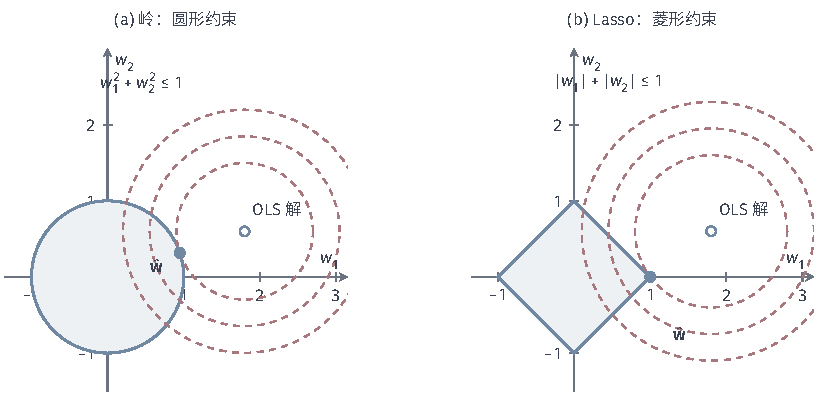
\includegraphics[width=138.649mm]{figures/03-models/01-classic-models/tikz/regression-regularization-geometry/figure.pdf}
  \caption{岭与Lasso的约束几何。构造损失为$J(\bm{w})=\lVert\bm{w}-(1.8,0.6)^{\top}\rVert_2^2/2$，虚线为等损失线，浅色区域为可行域，空心点为OLS解，实心点为约束最优解。左图解为$(1.8,0.6)^{\top}/\sqrt{3.6}$，右图解为$(1,0)^{\top}$。两图都取单位约束半径以比较形状，不表示相同的惩罚强度；Lasso也并非总在尖点取到最优解。}
  \label{fig:regression-regularization-geometry}
\end{figure*}

岭惩罚沿设计矩阵的谱方向收缩系数，一般设计下各原始坐标受到的相对收缩可以不同，下面将给出相应分解。惩罚的概率解释同样依赖归一化：高斯似然下，高斯先验对应二次惩罚，各系数独立的拉普拉斯先验（Laplace prior）对应一范数惩罚，但先验尺度与$\lambda$的对应关系还包含$n$和噪声方差。

\subsubsection{参数学习}
\label{sec:regression-regularization-learning}

岭目标的梯度为零给出
\begin{equation}
  \widehat{\bm{w}}_{\lambda}
  =(\bm{X}^{\top}\bm{X}+n\lambda\bm{I})^{-1}\bm{X}^{\top}\bm{y},
  \qquad\lambda>0.
  \label{eq:regression-ridge-solution}
\end{equation}
任意非零$\bm{v}$满足$\bm{v}^{\top}(\bm{X}^{\top}\bm{X}+n\lambda\bm{I})\bm{v}=\lVert\bm{X}\bm{v}\rVert_2^2+n\lambda\lVert\bm{v}\rVert_2^2>0$，所以即使设计秩亏，斜率解也唯一。若$\gamma_{\max},\gamma_{\min}$是$\bm{X}^{\top}\bm{X}$的极端特征值，正则化后该矩阵的条件数为$(\gamma_{\max}+n\lambda)/(\gamma_{\min}+n\lambda)$；比较对象是正规方程矩阵，而非$\bm{X}$本身的条件数。

取$\bm{X}=\bm{U}_r\bm{D}_r\bm{V}_r^{\top}$，正奇异值为$s_j$，则
\begin{equation}
  \bm{X}\widehat{\bm{w}}_{\lambda}
  =\sum_{j=1}^{r}\frac{s_j^2}{s_j^2+n\lambda}
       \bm{u}_j\bm{u}_j^{\top}\bm{y}.
  \label{eq:regression-ridge-spectral}
\end{equation}
OLS保留列空间中的全部投影，岭回归则按$s_j^2/(s_j^2+n\lambda)$保留各方向，小奇异值方向受到更强收缩。这是稳定性改善的来源，也说明惩罚会同时压低这些方向上的真实信号。

Lasso的目标记为$F(\bm{w})$。由于$\lambda>0$时$F(\bm{w})\geq\lambda\lVert\bm{w}\rVert_1$，连续目标至少取得一个最小值；参数解未必唯一。要理解零系数为何可能最优，可以先固定其他坐标。令$\bm{r}_{-j}=\bm{y}-\sum_{k\ne j}\bm{X}_{:,k}w_k$，$a_j=\lVert\bm{X}_{:,j}\rVert_2^2/n$、$c_j=\bm{X}_{:,j}^{\top}\bm{r}_{-j}/n$，略去常数后的单坐标目标为
\[
  q_j(w_j)=\frac{a_j}{2}w_j^2-c_jw_j+\lambda|w_j|.
\]
在零点左侧，绝对值项的斜率为$-\lambda$；右侧则为$\lambda$。因此零点的左右导数分别为
\[
  q'_{j,-}(0)=-c_j-\lambda,\qquad
  q'_{j,+}(0)=-c_j+\lambda.
\]
这个目标是凸函数，零点最优恰好要求左导数不大于零、右导数不小于零，即$|c_j|\leq\lambda$。此时无论向哪一侧离开零点，目标都不会降低；损失项在零点的导数$-c_j$却不必为零。

为了统一写出光滑点与尖点的条件，引入\term{次梯度}（subgradient）。对一维凸函数$f$，若斜率$s$满足$f(v)\geq f(u)+s(v-u)$对所有$v$成立，它就是$f$在$u$处的一个次梯度：经过该点、斜率为$s$的直线始终位于函数图像下方。所有这样的斜率组成次梯度集合$\partial f(u)$；可导时集合只有导数一个元素，而$|u|$在零点允许$[-1,1]$中的全部斜率。凸函数的最优性因而可统一表为$0\in\partial f(u)$。对Lasso，损失梯度加上惩罚次梯度为零，得到充要最优性条件
\begin{equation}
  \frac{\bm{X}^{\top}(\bm{y}-\bm{X}\widehat{\bm{w}})}{n}
  =\lambda\bm{z},\qquad
  z_j\in
  \begin{cases}
    \{\operatorname{sign}(\widehat w_j)\},&\widehat w_j\ne0,\\
    [-1,1],&\widehat w_j=0.
  \end{cases}
  \label{eq:regression-lasso-kkt}
\end{equation}
其中非零坐标对应的绝对值导数为符号函数，零坐标则允许整个区间来抵消损失梯度。沿用上述$a_j,c_j$，在正、负半轴求导，并在零点检验$|c_j|\leq\lambda$，得到坐标更新
\begin{equation}
  w_j\leftarrow\frac{\mathcal{S}_{\lambda}(c_j)}{a_j},
  \qquad
  \mathcal{S}_{\lambda}(c)=\operatorname{sign}(c)(|c|-\lambda)_+.
  \label{eq:regression-soft-threshold}
\end{equation}
这里$a_j>0$，零列直接取零系数。\term{软阈值}（soft thresholding）把阈值内的量置零，将其余量向零移动$\lambda$。例如正交标准化设计下，OLS系数$(0.12,1.40)$在$\lambda=0.20$时变为$(0,1.20)$；相关设计则需反复更新部分残差，不能直接阈值化OLS系数。循环坐标下降可用式\eqref{eq:regression-lasso-kkt}的违反程度作为停止依据。

弹性网的坐标更新为$\mathcal{S}_{\lambda_1}(c_j)/(a_j+\lambda_2)$。组惩罚则可用近端梯度：先令$\bm{v}=\bm{w}-t\bm{X}^{\top}(\bm{X}\bm{w}-\bm{y})/n$，再逐组计算
\begin{equation}
  \bm{w}_{A_g}^{+}
  =
  \begin{cases}
    \bm{0},&\lVert\bm{v}_{A_g}\rVert_2\leq t\lambda\omega_g,\\
    \left(1-\dfrac{t\lambda\omega_g}{\lVert\bm{v}_{A_g}\rVert_2}\right)
      \bm{v}_{A_g},&\text{其他情形}.
  \end{cases}
  \label{eq:regression-group-prox}
\end{equation}
该式求解的是$\min_{\bm{u}}\lVert\bm{u}-\bm{v}_{A_g}\rVert_2^2/2+t\lambda\omega_g\lVert\bm{u}\rVert_2$：固定$\lVert\bm{u}\rVert_2$时，同向选择使平方距离最小，剩下的一维非负半轴问题给出径向阈值。该闭式解针对欧氏距离构成的近端子问题；一般设计的块坐标子问题还包含组内设计的曲率，需要据此求解。对非零设计，取$0<t\leq1/\lVert\bm{X}^{\top}\bm{X}/n\rVert_2$可保证凸近端梯度法的目标收敛性质。

沿$\lambda$网格使用前一个解热启动，可以减少重复计算。LARS的Lasso修正版利用分段线性路径求解一范数惩罚问题，但这一性质不直接推广到一般Group Lasso。超参数通常由交叉验证选择；中心化、标准化与变量选择都必须在每个训练折内完成。跨软件比较超参数时，应先将平方损失与惩罚换算到相同的系数约定\scite{hastie2009}。

\subsubsection{理论分析}
\label{sec:regression-regularization-theory}

加入惩罚后，训练算法选择系数的方式和估计量的统计行为都会改变。凸性与步长决定优化能否到达目标最小值；惩罚对真实信号和噪声的同时收缩，决定偏差、方差以及变量选择。下面在固定设计下比较这些量，再为符号恢复单独规定噪声和最小信号条件。

\paragraph{表达能力}
岭回归在原线性函数族中偏好较小系数，Lasso进一步偏好零坐标；将惩罚换成硬范数约束时，允许选择的集合会直接缩小。约束越强，数据不足以确定的变化越难进入模型，目标中的真实弱信号也可能一同被压低。表示选择与正则强度因此需要一起评价。

\paragraph{收敛性}
凸性保证满足最优性条件的点是全局最优点，但迭代算法仍需合适的步长。岭回归在$\lambda>0$时具有正定Hessian，梯度下降可按前述谱条件选择步长；Lasso与组Lasso的近端更新则需同时处理光滑损失和非光滑惩罚。目标值收敛与参数解唯一是不同性质：岭与含正二次惩罚的弹性网有唯一斜率解，Lasso的唯一性还取决于设计和活跃坐标。

\paragraph{泛化性}
正则化的统计收益来自偏差与方差的取舍：收缩会压低参数的真实分量，也会减弱噪声引起的波动。下面的定理在固定设计与真参数下比较参数均方误差，说明足够小的正收缩可以使方差下降超过偏差平方的增加。这个比较对象是参数误差，预测风险还要由新输入怎样加权这些参数方向来决定。

\begin{figure}[htbp]
  \centering
  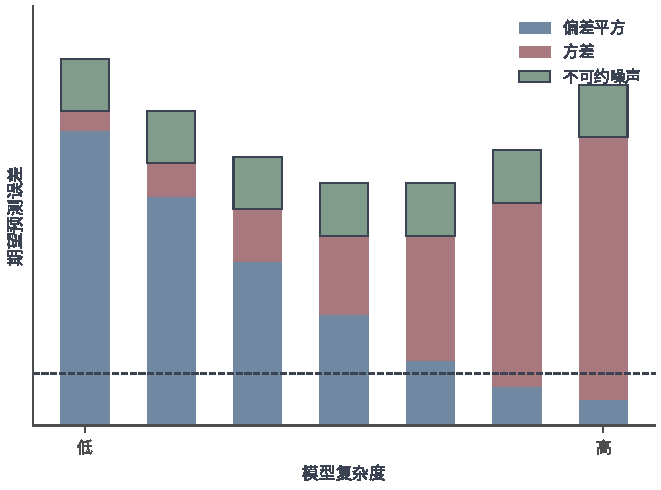
\includegraphics[width=105.412mm]{figures/03-models/01-classic-models/matplotlib/regression-bias-variance-noise/figure.pdf}
  \caption{模型复杂度变化时的偏差—方差—噪声分解示意。柱高是教学构造的相对量，不来自实验：复杂度增加时偏差平方下降、估计方差上升，不可约噪声保持不变。总误差由三部分共同决定，因此“模型更复杂”与“误差更小”都不是无条件结论。}
  \label{fig:regression-bias-variance-noise}
\end{figure}

\Needspace{8\baselineskip}
\begin{theorem}[小幅岭收缩的参数均方误差]
  \label{thm:regression-ridge-mse}
  设$\bm{y}=\bm{X}\bm{w}_{\star}+\bm{\varepsilon}$，固定设计$\bm{X}$列满秩，参数维数至少为$1$，噪声均值为零、协方差为$\sigma^2\bm{I}$，且$\sigma^2>0$。则存在$\lambda_0>0$，使所有$0<\lambda<\lambda_0$的岭估计参数均方误差严格小于OLS。
\end{theorem}

\begin{proof}
令$a=n\lambda$，将$\bm{X}^{\top}\bm{X}$正交对角化，特征值为$\gamma_j>0$，真参数在相应方向上的坐标为$\theta_j$。岭估计在第$j$个方向上的偏差为$-a\theta_j/(\gamma_j+a)$，方差为$\sigma^2\gamma_j/(\gamma_j+a)^2$。正交变换保持欧氏范数，故参数均方误差为
\[
  M(a)=\sum_j\frac{a^2\theta_j^2+\sigma^2\gamma_j}{(\gamma_j+a)^2}.
\]
函数在$a=0$附近可微，且$M'(0)=-2\sigma^2\sum_j\gamma_j^{-2}<0$。导数定义保证存在$a_0>0$，使所有$0<a<a_0$满足$M(a)<M(0)$。取$\lambda_0=a_0/n$即可。
\end{proof}

中心化响应会使噪声协方差变成$\sigma^2(\bm{I}-\bm{1}\bm{1}^{\top}/n)$，但中心化设计满足$\bm{X}^{\top}\bm{1}=\bm{0}$，所以斜率方向上的上述计算仍成立。定理中的有效收缩范围依赖真参数；实际正则强度仍需选择，预测风险还需按测试输入对参数方向的加权来评价。

Lasso能否认出真实非零变量，则是更强的问题。仅有稀疏性还不够：无关变量若可由相关变量近似替代，就难以判定贡献应归给谁。\term{不可表示条件}（irrepresentable condition）限制这种替代关系；符号恢复还需要噪声和最小信号条件\scite{zhao2006lasso}。

\Needspace{18\baselineskip}
\begin{theorem}[Lasso的确定性符号恢复充分条件]
  \label{thm:regression-lasso-recovery}
  设$\bm{y}=\bm{X}\bm{w}_{\star}+\bm{\varepsilon}$，$A=\{j:w_{\star,j}\ne0\}$非空，$\bm{X}_A=\bm{X}_{:,A}$列满秩。记
  \[
    \bm{G}=\bm{X}^{\top}\bm{X}/n,\quad
    \bm{s}=\operatorname{sign}(\bm{w}_{\star,A}),\quad
    \bm{P}_A=\bm{X}_A(\bm{X}_A^{\top}\bm{X}_A)^{-1}\bm{X}_A^{\top},
  \]
  以及$\bm{q}=\bm{G}_{A,A}^{-1}\bm{X}_A^{\top}\bm{\varepsilon}/n$、$\bm{b}=\bm{G}_{A,A}^{-1}\bm{s}$。若$\lambda>0$，且存在$0<\eta\leq1$使
  \begin{align}
    \lVert\bm{G}_{A^c,A}\bm{G}_{A,A}^{-1}\bm{s}\rVert_\infty
      &\leq1-\eta, \label{eq:regression-irrepresentable}\\
    \left\lVert\bm{X}_{A^c}^{\top}(\bm{I}-\bm{P}_A)
                  \bm{\varepsilon}/n\right\rVert_\infty
      &\leq\lambda\eta/2, \label{eq:regression-lasso-noise}\\
    \min_{j\in A}|w_{\star,j}|
      &>\lVert\bm{q}\rVert_\infty+\lambda\lVert\bm{b}\rVert_\infty,
      \label{eq:regression-lasso-beta-min}
  \end{align}
  则Lasso解唯一，且$\operatorname{sign}(\widehat{\bm{w}})=\operatorname{sign}(\bm{w}_{\star})$。$A^c$为空时，前两个条件为空条件。
\end{theorem}

\begin{proof}
构造$\widetilde{\bm{w}}_{A^c}=\bm{0}$、$\widetilde{\bm{w}}_A=\bm{w}_{\star,A}+\bm{q}-\lambda\bm{b}$。最小信号条件保证每个活跃坐标的扰动小于其原绝对值，因此符号仍为$\bm{s}$。残差满足
\[
  \bm{r}=\bm{y}-\bm{X}\widetilde{\bm{w}}
  =(\bm{I}-\bm{P}_A)\bm{\varepsilon}
   +\lambda\bm{X}_A\bm{G}_{A,A}^{-1}\bm{s}.
\]
令$\widetilde{\bm{z}}=\bm{X}^{\top}\bm{r}/(n\lambda)$，则$\widetilde{\bm{z}}_A=\bm{s}$，且
\[
  \widetilde{\bm{z}}_{A^c}
  =\bm{G}_{A^c,A}\bm{G}_{A,A}^{-1}\bm{s}
    +\frac{\bm{X}_{A^c}^{\top}(\bm{I}-\bm{P}_A)
            \bm{\varepsilon}}{n\lambda}.
\]
前两个条件给出$\lVert\widetilde{\bm{z}}_{A^c}\rVert_\infty\leq1-\eta/2<1$。因此$\widetilde{\bm{z}}$是合法次梯度，式\eqref{eq:regression-lasso-kkt}成立，候选解最优。

对任意扰动$\bm{h}$，精确展开目标差并代入平稳条件，得到
\[
  \begin{aligned}
    F(\widetilde{\bm{w}}+\bm{h})-F(\widetilde{\bm{w}})
    ={}&\frac{\lVert\bm{X}\bm{h}\rVert_2^2}{2n}\\
      &+\lambda\bigl(\lVert\widetilde{\bm{w}}+\bm{h}\rVert_1
         -\lVert\widetilde{\bm{w}}\rVert_1
         -\widetilde{\bm{z}}^{\top}\bm{h}\bigr).
  \end{aligned}
\]
活跃坐标的括号贡献由次梯度不等式非负；非活跃坐标的贡献至少为$(\eta/2)|h_j|$。若扰动后仍最优，必有$\bm{h}_{A^c}=\bm{0}$与$\bm{X}\bm{h}=\bm{0}$，故$\bm{X}_A\bm{h}_A=\bm{0}$。活跃设计满列秩进一步推出$\bm{h}_A=\bm{0}$，唯一性得证。
\end{proof}

这个命题直接约束一份数据中的噪声向量，不需要高斯假设。要得到高概率恢复，还须对这些约束的概率作估计。例如在固定设计、独立高斯噪声且$\lVert\bm{X}_{:,j}\rVert_2\leq\sqrt n$下，并合界给出
\[
  \mathbb{P}\!\left(
    \lVert\bm{X}_{A^c}^{\top}(\bm{I}-\bm{P}_A)
       \bm{\varepsilon}/n\rVert_\infty>\lambda\eta/2
  \right)
  \leq2|A^c|\exp\!\left(-\frac{n\lambda^2\eta^2}{8\sigma^2}\right).
\]
完整恢复结论还需控制活跃坐标上的$\bm{q}$，以验证最小信号条件。变量选择与预测误差关注的对象也不同：相关特征之间的替换可能保持近似相同的预测，却改变支持集；若要进一步解释干预效应，还需要因果模型和识别条件。

\subsubsection{支持相关特征的分组稳定（Elastic Net）}
\label{sec:regression-elastic-net}

弹性网中的$\lambda_2>0$使整个目标严格凸，即使设计秩亏也有唯一参数解。若两列完全相同，交换相应系数不改变目标，唯一性便要求两个系数相等。二次惩罚由此排除了完全相同特征之间任意分摊系数的歧义。

对两个非零且同号的系数，把各自的最优性条件相减，可得
\[
  \lambda_2|\widehat w_j-\widehat w_k|
  \leq\frac{\lVert\bm{X}_{:,j}-\bm{X}_{:,k}\rVert_2
                  \lVert\bm{y}-\bm{X}\widehat{\bm{w}}\rVert_2}{n}.
\]
因此在相同尺度下，两列越接近，其同号估计越接近。这个界以非零同号为条件，不保证任何相关变量组都被选中。实际选择$\alpha,\lambda$时，仍应根据预测或变量选择的目标验证稳定性。

\subsubsection{支持结构化稀疏（Group Lasso）}
\label{sec:regression-group-lasso}

一个类别变量的多个指示变量，或一个连续变量的整组样条基，常需要作为整体评价。组Lasso把这样的先验分组写进惩罚；在非零组上，惩罚的梯度方向是$\bm{w}_{A_g}/\lVert\bm{w}_{A_g}\rVert_2$，零组处的次梯度则是单位球。组内残差相关向量未超过$\lambda\omega_g$时，整组可以保持为零。

权重$\sqrt{|A_g|}$能补偿组大小的一部分影响，但并不消除组内相关性或量纲差异。若还希望在保留组内继续选择坐标，可使用\term{稀疏组Lasso}（sparse group Lasso），即在组惩罚之外再加$\lambda_1\lVert\bm{w}\rVert_1$。这同时约束组与坐标两个层次；选择一致性除真实组结构外，还依赖设计、信号强度及正则化条件。

\subsubsection{小结}
\label{sec:regression-regularization-summary}

岭回归收缩全部系数，Lasso选择坐标，弹性网同时利用坐标选择与二次收缩，组Lasso则将选择单位改为预先给定的变量组。它们的差别来自希望保留的参数结构，求解与恢复结论也要匹配相应惩罚。其他方法沿着这些选择继续扩展：Adaptive Lasso按坐标加权，Fused Lasso惩罚相邻系数差，SCAD和MCP减弱对大系数的收缩。后两者采用非凸惩罚，需要处理局部最优；所称“Oracle性质”也只在规定的渐近条件下，描述仿佛已知真支持集的估计行为\scite{hastie2009}。

处理共线性的另一条路线是先降维再回归。\term{主成分回归}（principal component regression, PCR）保留若干主成分，在这些正交方向上拟合，等价于对选中方向完全保留、对其余方向硬截断。第\ref{sec:dim-pca}节从无监督表示的角度推导主成分分析（PCA）：PCA与PCR共享由输入方差确定的主成分基，但PCA按方差保留与重构误差评价表示，PCR还要用响应检验这些成分是否有利于预测。与式\eqref{eq:regression-ridge-spectral}的连续收缩相比，PCR的取舍更直接，但输入方差小不意味着对响应不重要。\term{偏最小二乘回归}（partial least squares regression, PLS）在构造成分时同时利用输入与响应的关系，因而属于监督降维；它有不同的具体算法，不能笼统理解为收缩因子必在$0$和$1$之间的岭回归。成分数同样需要在训练折内选择。

\subsection{分位数回归（Quantile Regression）}
\label{sec:regression-quantiles}

预算制定者关心的是实际支出超过预算的概率，单个条件均值无法回答这个问题。\term{分位数回归}（quantile regression）用非对称残差损失估计给定输入后的指定分位数；例如$0.9$分位数提供一个使响应至少有$90\%$概率不超过它的条件阈值。Koenker与Bassett在1978年系统提出回归分位数，将回归目标从条件均值扩展到条件分布的不同位置。这一区分源于决策目标，无需先假定误差对称或同方差\scite{koenker1978quantiles}。

\subsubsection{模型结构}

预算阈值低估时产生超支，高估时则预留过多；两种偏差的代价可以不同。给定$0<\tau<1$，\term{分位数损失}（pinball loss）用$\tau$和$1-\tau$分别给正、负残差计分：
\begin{equation}
  \rho_\tau(r)=
  \begin{cases}
    \tau r,&r\geq0,\\
    (1-\tau)(-r),&r<0.
  \end{cases}
  \label{eq:regression-pinball}
\end{equation}
残差仍取$r=y-\widehat y$，所以较大的$\tau$更重地惩罚低估。线性分位数回归最小化$\sum_i\rho_\tau(y_i-\bm\phi(\bm x_i)^\top\bm w)$。这一非对称损失以分位数作为总体最优预测：对前面固定的$0<\tau<1$，若$\mathbb E|Y|<\infty$，记响应分布函数为$F_Y$，则$Q(a)=\mathbb E[\rho_\tau(Y-a)]$的全部最小点恰好满足
\[
 F_Y(a-)\leq\tau\leq F_Y(a),
 \qquad F_Y(a-)=\mathbb P(Y<a).
\]
左右不等式来自该凸损失关于预测值的单侧导数；在原子或平台处，它们保留了可能不唯一的最优点集合（参考\BookSectionRef{sec:statistics-nonparametric-missing}{第一卷“数学准备”的“分布与条件函数的估计”小节}）。

将分布换成给定输入的条件分布，便得到条件分位数；换成经验分布，便得到样本分位数。$\tau=1/2$时损失为$|r|/2$，对应中位数。在线性模型受到限制时，只有正确指定等条件下才能精确表示真实条件分位数，一般得到该函数类中的最佳损失逼近。

\subsubsection{参数学习}

引入非负正、负残差$\bm{u},\bm{v}\in\mathbb{R}^{n}$，可将目标写成线性规划
\begin{equation}
  \begin{aligned}
    \min_{\bm{w},\bm{u},\bm{v}}\quad&
      \tau\bm{1}^{\top}\bm{u}+(1-\tau)\bm{1}^{\top}\bm{v},\\
    \text{满足}\quad&
      \bm{y}-\bm{X}\bm{w}=\bm{u}-\bm{v},
      \quad\bm{u}\geq\bm{0},\ \bm{v}\geq\bm{0}.
  \end{aligned}
  \label{eq:regression-quantile-lp}
\end{equation}
若某个$u_i,v_i$同时为正，同时减小二者保持约束不变且严格降低目标，因此最优时二者不会同时为正，线性规划与原损失等价。可采用单纯形法、内点法或适合数据规模的非光滑凸优化算法；这些算法分别利用线性规划结构或直接处理非光滑凸目标。

高维时可在平均分位数损失之外增加$\lambda\lVert\bm{w}\rVert_1$，通过把系数也拆为正负部分继续写成线性规划。多个$\tau$可以分别拟合，也可以联合加入顺序约束；超参数评价应使用对应的分位数损失，而不是仅凭平方误差判断。

\subsubsection{小结}

分位数回归把预测从条件均值扩展到分布中的指定位置，多个分位数有助于描述分布形状，但有限网格不等于完整条件分布。独立拟合可能出现较高分位数反而更低的分位数交叉，联合约束需说明在哪些输入上生效。线性尾部损失降低了大残差的边际作用，却不自动抵御高杠杆点；极端分位数仍需要足够尾部数据。预测区间由分位数组成后，其覆盖率也需要单独评价。

\subsection{支持向量回归（SVR）}
\label{sec:regression-svr}

另一种误差评价允许小偏差不计损失，只惩罚超出容忍范围的部分。\term{支持向量回归}（support vector regression, SVR）将这种损失与二次正则化结合，得到一个由训练样本加权表示的预测函数。部分样本的权重可以为零，核化以后只需保留非零权重对应的样本来计算预测。这是样本展开的稀疏性，与Lasso选择输入变量的稀疏性不同\scite{smola2004svr}。

\subsubsection{模型结构}

设$\epsilon\geq0$，定义\term{$\epsilon$不敏感损失}（$\epsilon$-insensitive loss）为$L_\epsilon(r)=(|r|-\epsilon)_+$。它把$\pm\epsilon$之间的残差视为可容忍误差，超出部分线性计入损失。线性SVR单独保留不受惩罚的截距$b$，目标为
\begin{equation}
  \min_{\bm{w},b}\;
    \frac12\lVert\bm{w}\rVert_2^2+
    C\sum_{i=1}^{n}L_\epsilon(y_i-\bm{w}^{\top}\bm{x}_i-b),
    \qquad C>0.
  \label{eq:regression-svr-objective}
\end{equation}
除以$nC$，可知它与“平均损失$+\lambda\lVert\bm{w}\rVert_2^2/2$”在$\lambda=1/(nC)$时等价。$C$越大，训练误差在目标中的相对权重越大；$\epsilon$则具有响应的单位，规定不计损失的范围。

为推导对偶问题，引入$\xi_i^+,\xi_i^-\geq0$，分别表示两个方向超出容忍带的量。等价约束形式为
\begin{equation}
  \begin{aligned}
    \min_{\bm{w},b,\bm{\xi}^+,\bm{\xi}^-}\quad&
       \tfrac12\lVert\bm{w}\rVert_2^2+C\sum_i(\xi_i^++\xi_i^-),\\
    \text{满足}\quad&
       y_i-\bm{w}^{\top}\bm{x}_i-b\leq\epsilon+\xi_i^+,\\
      &\bm{w}^{\top}\bm{x}_i+b-y_i\leq\epsilon+\xi_i^-,\\
      &\xi_i^+,\xi_i^-\geq0,\qquad i=1,\ldots,n.
  \end{aligned}
  \label{eq:regression-svr-primal}
\end{equation}
固定预测时，由$C>0$可知最优松弛量恰为超出带宽的部分。$\epsilon=0$对应带二次惩罚的绝对损失回归。对固定有限数据，若$\epsilon\geq(\max_i y_i-\min_i y_i)/2$，则$\bm{w}=\bm{0}$和某个常数$b$已能使全部样本进入容忍带，目标取得零值。截距在此时可能不唯一。

\subsubsection{参数学习}

原问题是在可行参数中寻找最小目标值，为什么下面会出现一个最大化问题？把各不等式写成“左边不大于零”，分别乘以非负的拉格朗日乘子并加到目标中，就得到拉格朗日函数。在任一可行点，这些附加项都不大于零；固定乘子，再对全部原始变量取下确界，便得到原问题最优值的一个下界。选择乘子把这个下界尽量抬高，就是\term{对偶}（dual）最大化。乘子在这里用于构造下界；若最佳下界等于原问题的最小值，就称为\term{强对偶}（strong duality）。

下面用凸优化条件判断这一对应何时成立。Slater条件要求在满足等式约束的同时存在严格可行的不等式点，它在当前凸问题中用于建立强对偶；KKT条件把原始可行性、对偶可行性、驻点条件和互补松弛放在同一组方程中，其中互补松弛要求乘子与对应约束余量的乘积为零。在凸问题满足Slater条件时，KKT条件对最优性既必要又充分；分类SVM中的对应条件见式\eqref{eq:classification-svm-hard-kkt}。

为前两组约束引入乘子$\alpha_i^+,\alpha_i^-\geq0$，为松弛量非负约束引入$\mu_i^+,\mu_i^-\geq0$。令$r_i=y_i-\bm{w}^{\top}\bm{x}_i-b$，拉格朗日函数为
\[
  \begin{aligned}
    \mathcal{L}={}&\tfrac12\lVert\bm{w}\rVert_2^2
       +C\sum_i(\xi_i^++\xi_i^-)
       +\sum_i\alpha_i^+(r_i-\epsilon-\xi_i^+)\\
       &+\sum_i\alpha_i^-(-r_i-\epsilon-\xi_i^-)
       -\sum_i(\mu_i^+\xi_i^++\mu_i^-\xi_i^-).
  \end{aligned}
\]
分别对$\bm{w},b,\xi_i^\pm$求导，得到
\[
  \bm{w}=\sum_i(\alpha_i^+-\alpha_i^-)\bm{x}_i,\qquad
  \sum_i(\alpha_i^+-\alpha_i^-)=0,\qquad
  C-\alpha_i^\pm-\mu_i^\pm=0.
\]
最后一式给出$0\leq\alpha_i^\pm\leq C$。记$\beta_i=\alpha_i^+-\alpha_i^-$，消去原始变量后，对偶问题为
\begin{equation}
  \begin{aligned}
    \max_{\bm{\alpha}^+,\bm{\alpha}^-}\quad&
       -\tfrac12\sum_{i,j}\beta_i\beta_j\bm{x}_i^{\top}\bm{x}_j
       -\epsilon\sum_i(\alpha_i^++\alpha_i^-)
       +\sum_i y_i\beta_i,\\
    \text{满足}\quad&
       \sum_i\beta_i=0,\qquad 0\leq\alpha_i^\pm\leq C.
  \end{aligned}
  \label{eq:regression-svr-dual}
\end{equation}
原始问题凸，选择足够大的正松弛量即可严格满足不等式，因此满足Slater条件，强对偶成立。对偶是带盒约束与一个线性等式约束的凸二次规划的最大化写法，可通过分解算法逐步更新少量变量；每次更新应保持等式约束，并以最优性残差作为停止依据。

得到乘子后，若$0<\alpha_i^+<C$，互补松弛给出$r_i=\epsilon$，所以$b=y_i-\bm{w}^{\top}\bm{x}_i-\epsilon$；若$0<\alpha_i^-<C$，则$b=y_i-\bm{w}^{\top}\bm{x}_i+\epsilon$。可对多个此类样本的截距估计取平均以减小数值误差。若没有内点乘子，应根据全部KKT不等式求可行截距区间，不能假设总能找到一个严格介于$0$与$C$之间的乘子。

\subsubsection{理论分析}

SVR的对偶给出了当前训练目标的最优性判据，接下来还要检查这个目标能表示什么、算法如何减少优化误差，以及训练样本怎样约束新输入上的误差。前两项由核函数、KKT条件和对偶间隙描述；泛化分析则另外需要抽样制度、函数类以及响应尾部条件。支持向量的数量是学得表示的规模，并非新样本风险的替代指标。

\paragraph{表达能力}
选定核以后，SVR在相应再生核Hilbert空间中拟合函数；非线性变化由核的特征映射提供。范数惩罚使某些变化比其他变化代价更大，$\varepsilon$不敏感损失则规定什么残差值得继续拟合。两者分别限制候选函数的变化方式和拟合精度，需要与目标规律匹配。

\paragraph{收敛性}
SVR的原始问题是凸优化问题，前述强对偶与KKT条件给出了全局最优性的判据。数值求解时，可以用原始可行解与对偶可行解的目标差距控制尚未消除的优化误差；具体迭代的收敛速度仍取决于求解器、设计与核矩阵。

支持向量与残差位置的关系必须区分带内、带外和边界三个情况。边界上的约束虽然取等号，乘子仍然可以为零。

\Needspace{16\baselineskip}
\begin{theorem}[SVR的样本系数与残差]
  \label{thm:regression-svr-support}
  设$\epsilon>0$，在任意一组原始与对偶最优解处记$r_i=y_i-\bm{w}^{\top}\bm{x}_i-b$、$\beta_i=\alpha_i^+-\alpha_i^-$。则
  \[
    \begin{array}{c|c}
      \text{残差位置}&\text{对偶乘子}\\ \hline
      |r_i|<\epsilon&\alpha_i^+=\alpha_i^-=0\\
      r_i>\epsilon&\alpha_i^+=C,\ \alpha_i^-=0\\
      r_i<-\epsilon&\alpha_i^+=0,\ \alpha_i^-=C\\
      r_i=\epsilon&\alpha_i^+\in[0,C],\ \alpha_i^-=0\\
      r_i=-\epsilon&\alpha_i^+=0,\ \alpha_i^-\in[0,C]
    \end{array}
  \]
  因而$\beta_i\ne0$蕴含$|r_i|\geq\epsilon$，反向蕴含在边界处不成立。
\end{theorem}

\begin{proof}
最优松弛量为$\xi_i^+=(r_i-\epsilon)_+$、$\xi_i^-=(-r_i-\epsilon)_+$。KKT互补松弛条件为
\[
  \alpha_i^+(\epsilon+\xi_i^+-r_i)=0,\qquad
  \alpha_i^-(\epsilon+\xi_i^-+r_i)=0,\qquad
  (C-\alpha_i^\pm)\xi_i^\pm=0.
\]
严格带内时两个残差约束都松弛，故两个乘子均为零。若$r_i>\epsilon$，则$\xi_i^+>0$迫使$\alpha_i^+=C$，另一个残差约束严格松弛，故$\alpha_i^-=0$；负向带外同理。若$r_i=\epsilon$，正向松弛量为零，其乘子仅受盒约束限制；由于$\epsilon>0$，负向残差约束严格松弛，故$\alpha_i^-=0$。另一侧边界同理。
\end{proof}

一个反例足以排除边界处的“当且仅当”：取单个样本、$\bm{x}_1=\bm{0}$，令$\bm{w}=\bm{0}$、$b=y_1-\epsilon$，则$r_1=\epsilon$，原始目标为零；两个乘子均为零也满足对偶最优性。这个边界样本的系数为零。$\epsilon=0$时两个边界重合，零残差处两类乘子可能同时非零，必须单独处理，不能沿用上表的两行边界结论。

\paragraph{泛化性}
支持向量的数量由最优函数与残差位置共同决定。改变$\epsilon$会重新拟合整条函数，因而支持向量数未必严格单调下降。泛化分析更直接地约束核对角线、函数范数、截距或响应尾部，并在指定抽样条件下评价新样本损失。有限步求解留下的优化误差，与有限数据造成的统计误差，分别进入这一评价。

\subsubsection{支持非线性回归（核 SVR）}
\label{sec:regression-kernel-svr}

当数值响应包含原始特征的非线性变化时，可以保留SVR的容忍带和范数惩罚，只改变用于计算内积的表示。采用第\ref{sec:classic-overview-kernel-trick}节的正定核$K$，把式\eqref{eq:regression-svr-dual}中的$\bm{x}_i^{\top}\bm{x}_j$换为$K(\bm{x}_i,\bm{x}_j)$，便得到特征空间中的同一个SVR对偶问题。预测为
\begin{equation}
  f(\bm{x})=\sum_{i=1}^{n}\beta_i K(\bm{x}_i,\bm{x})+b.
  \label{eq:regression-kernel-svr-prediction}
\end{equation}
核函数及其合法性见第\ref{sec:classic-overview-kernel-validity}节与第\ref{sec:classic-overview-common-kernels}节。核决定表示，$\epsilon$不敏感响应损失与系数约束决定回归学习的目标；这也使核SVR与使用分类间隔损失的核SVM承担不同任务。

核SVR沿用相同的对偶结构，但计算规模从显式特征维数转向训练样本数。核矩阵若完整保存需要$O(n^2)$空间，采用缓存可以降低内存占用；训练时间还依赖求解器、精度及数据条件。预测需要约$n_{\mathrm{SV}}$次核计算，其中$n_{\mathrm{SV}}$为非零展开系数的样本数。线性核则可预先合并$\bm{w}$，使预测成本恢复为$O(d)$。

\subsubsection{小结}

SVR在固定容忍带下折中残差代价与函数范数，核化使这种折中作用于非线性函数类。这一目标得到的是容忍带下的点预测；要估计指定条件分位数或完整分布，还需要相应损失或概率设定。$\nu$-SVR通过另一个参数控制与误差比例、支持向量比例有关的约束，具体比例结论有相应条件；最小二乘SVR把损失换为平方形式，与核岭回归密切相关，但是否惩罚截距必须一致后才能判断等价。核选择与$C,\epsilon$调参共同影响结果，方法是否适用应按样本展开规模、验证误差及预算判断。

\subsection{广义线性模型（GLM）}
\label{sec:regression-glm}

预测每天的交易次数时，均值必须非负；预测交易是否成功时，均值是$[0,1]$中的概率。平方损失可以用于这些响应，但无约束线性预测不自动满足取值范围，也没有规定均值与方差的关系。\term{广义线性模型}（generalized linear model, GLM）把响应分布、均值和线性预测器连接起来。Nelder与Wedderburn在1972年给出这一统一框架，使高斯、二项和Poisson等响应可以沿同一条似然与加权最小二乘路线处理；扩展的关键是响应分布与链接，而不只是增加多项式特征\scite{nelder1972glm}。

\subsubsection{模型结构}

条件于输入，假设响应相互独立，密度或概率质量函数具有指数族形式
\begin{equation}
  p(y_i\mid\theta_i,\varphi)
  =\exp\!\left\{
    \frac{y_i\theta_i-b(\theta_i)}{a(\varphi)}
    +c(y_i,\varphi)\right\},\qquad a(\varphi)>0.
  \label{eq:regression-exponential-family}
\end{equation}
$\theta_i$是自然参数，$\varphi$是离散度参数或尺度参数；此处为便于推导，所有观测使用相同的$a(\varphi)$。函数$a,b,c$的形式由选定的分布族确定，并不作为三个未知函数一起学习。例如，均值为$\mu_i>0$的Poisson分布可写成
\[
  p(y_i\mid\mu_i)
  =\frac{\mu_i^{y_i}e^{-\mu_i}}{y_i!}
  =\exp\{y_i\log\mu_i-\mu_i-\log(y_i!)\}.
\]
逐项对照式\eqref{eq:regression-exponential-family}，可得$\theta_i=\log\mu_i$、$b(\theta_i)=e^{\theta_i}$、$a(\varphi)=1$、$c(y_i,\varphi)=-\log(y_i!)$。这里没有额外待估的离散度参数，自然参数也不是均值本身。

一般情形下，假定支持集不随$\theta_i$改变，并允许交换积分（离散情形为求和）与微分。密度积分为$1$，对$\theta_i$求导得到$\mathbb{E}[Y_i-b'(\theta_i)]=0$；再求一次导数得到
\[
  \mathbb{E}\!\left[
    \frac{(Y_i-b'(\theta_i))^2}{a(\varphi)^2}
      -\frac{b''(\theta_i)}{a(\varphi)}\right]=0.
\]
因此均值与方差为
\begin{equation}
  \mu_i=b'(\theta_i),\qquad
  \operatorname{Var}(Y_i\mid\bm{x}_i)
  =a(\varphi)b''(\theta_i)=a(\varphi)V(\mu_i).
  \label{eq:regression-glm-moments}
\end{equation}
函数$V$描述方差怎样随均值变化。GLM再引入线性预测器$\eta_i=\bm{\phi}(\bm{x}_i)^{\top}\bm{w}$与\term{链接函数}（link function）$g$，令$g(\mu_i)=\eta_i$。链接作用于条件均值，而不是把每个观测$y_i$变换后做OLS。若$\eta_i=\theta_i$，称为规范链接。

表\ref{tab:regression-glm}列出三种基本组合。伯努利模型的均值就是成功概率，因此logistic回归既可作为概率回归理解，也可在给定决策阈值后用于分类。第\ref{sec:classification-logistic}节沿用伯努利似然、logit链接与IRLS计算，但把重点转向类别标签的概率、决策阈值与校准；本节则借这一特例说明GLM中响应分布、链接和均值方差关系的共同结构。Poisson模型采用对数链接，使$\mu_i=\exp(\eta_i)>0$；响应是整数，条件均值却不必为整数。

\begin{table}[htbp]
  \centering
  \begin{tabular}{llll}
    \toprule
    响应模型 & $b(\theta)$ & 规范链接$g(\mu)$ & $V(\mu)$\\
    \midrule
    高斯 & $\theta^2/2$ & $\mu$ & $1$\\
    伯努利 & $\log(1+e^\theta)$ & $\log\frac{\mu}{1-\mu}$ & $\mu(1-\mu)$\\
    Poisson & $e^\theta$ & $\log\mu$ & $\mu$\\
    \bottomrule
  \end{tabular}
  \caption{GLM的三个常用特例。高斯模型的$a(\varphi)=\sigma^2$，后两者的$a(\varphi)=1$。链接保证均值范围，分布假设进一步规定条件方差。}
  \label{tab:regression-glm}
\end{table}

二项分布可处理已知试验次数下的成功数；Gamma模型可处理正连续响应。链接选择并不唯一，必须同时满足自然参数域和均值域的要求。Poisson的均值方差相等也可能与数据不符，过度离散、零膨胀或观测相关性需要额外建模，不能靠对数链接本身解决。

\subsubsection{参数学习}

记$\bm{z}_i=\bm{\phi}(\bm{x}_i)$，设计矩阵第$i$行为$\bm{z}_i^{\top}$，暂将$\varphi$视为已知。由$d\mu_i/d\theta_i=V(\mu_i)$及$d\eta_i/d\mu_i=g'(\mu_i)$，对数似然的得分为
\begin{equation}
  \bm{U}(\bm{w})
  =\sum_i\frac{y_i-\mu_i}
    {a(\varphi)V(\mu_i)g'(\mu_i)}\bm{z}_i.
  \label{eq:regression-glm-score}
\end{equation}
在所需导数存在且$g'(\mu_i)\ne0$时，期望负Hessian即Fisher信息$\bm{X}^{\top}\bm{W}\bm{X}$，其中
\[
  W_{i,i}=\frac{1}{a(\varphi)V(\mu_i)[g'(\mu_i)]^2}.
\]
\term{Fisher评分}（Fisher scoring）用这个期望曲率修正当前参数，更新$\bm{w}^{+}=\bm{w}+(\bm{X}^{\top}\bm{W}\bm{X})^{-1}\bm{U}(\bm{w})$。要把它写成加权最小二乘，需要先把响应尺度上的误差换算成线性预测器尺度上的修正。在当前均值附近，链接函数的一阶近似为$g(\mu_i+\Delta\mu)\approx\eta_i+g'(\mu_i)\Delta\mu$；将残差$y_i-\mu_i$作为局部修正信号，便得到\term{工作响应}（working response）
\[
  z_i^{\mathrm{work}}
    =\eta_i+(y_i-\mu_i)g'(\mu_i),
\]
它是本轮局部子问题的目标值，会随当前参数改变，并非把真实标签永久变成$g(y_i)$。固定当前参数时，这个仿射换算后的响应方差为$a(\varphi)V(\mu_i)[g'(\mu_i)]^2$，其倒数正是$W_{i,i}$；换算后方差较大的观测因而权重较小。代入可得$\bm{U}=\bm{X}^{\top}\bm{W}(\bm{z}^{\mathrm{work}}-\bm{X}\bm{w})$，从而
\begin{equation}
  \bm{w}^{+}
  =(\bm{X}^{\top}\bm{W}\bm{X})^{-1}
     \bm{X}^{\top}\bm{W}\bm{z}^{\mathrm{work}}.
  \label{eq:regression-irls}
\end{equation}
这就是\term{迭代重加权最小二乘}（iteratively reweighted least squares, IRLS）：在当前均值附近构造一个加权平方子问题。实际使用分解求解线性方程，检查秩、参数域与似然下降情况，必要时采用阻尼或线搜索。各观测共享的$a(\varphi)$在无惩罚参数更新中可以约去，但在信息矩阵和方差计算中不能遗漏。

规范链接下，$\theta_i=\eta_i$，负对数似然的Hessian为
\[
  \frac{1}{a(\varphi)}
  \bm{X}^{\top}\operatorname{diag}(b''(\eta_i))\bm{X}.
\]
它半正定，因此目标凸；若$b''(\eta_i)>0$且设计列满秩，则有限参数域内严格凸。这时Newton法与Fisher评分具有相同的曲率矩阵，但完整步长不自动保证每次都提高似然，更不能保证有限最优解存在。

\subsubsection{理论分析}
\label{sec:regression-glm-theory}

采用GLM以后，响应分布与链接同时规定了候选均值和似然目标。分析需要从这里分开：候选均值能否描述输入作用，固定样本是否存在有限最大似然解，求得的估计量在重复抽样中怎样变化。渐近分布的讨论以模型正确、维数固定以及相应抽样和正则条件为前提，所得参数区间也要与未来响应的预测区间区分。

\paragraph{表达能力}
GLM先用线性预测器组合特征，再经逆链接得到均值，并用响应分布规定条件方差。错误链接或遗漏交互会使真实均值落在候选关系之外；样本增加可以减少估计误差，拟合中这种表示失配仍然存在。

\paragraph{收敛性}
严格凸性只能保证已经存在的最优解唯一。以无惩罚logistic回归为例，若存在方向$\bm{v}$使类别标签$t_i\in\{-1,1\}$满足$t_i\bm{z}_i^{\top}\bm{v}>0$，则负对数似然$\sum_i\log(1+\exp(-t_i\bm{z}_i^{\top}\bm{w}))$在$\bm{w}=a\bm{v}$、$a\to\infty$时趋于零，却在每个有限参数处严格为正。即使设计满秩，也没有有限最大似然估计。分离、近似分离和病态设计都可能使迭代参数持续增大。

\paragraph{泛化性}
有限样本估计量的分布可以帮助量化参数及预测的不确定性，它与优化算法的收敛分别分析。以下给出统计渐近分布的一组充分条件；具体GLM需根据分布、链接和输入矩条件验证它们。

设观测独立同分布，模型正确指定，参数维数固定，真参数$\bm w_\star$位于参数域内部。单样本对数似然$\ell_i(\bm w)$在真参数的某凸邻域内二阶连续可微，并满足
\[
 \mathbb E[\nabla\ell_i(\bm w_\star)]=\bm0,\qquad
 \operatorname{Cov}(\nabla\ell_i(\bm w_\star))
 =\bm I_\star\succ0.
\]
再假设有限的内部最大似然估计$\widehat{\bm w}_n$以趋于$1$的概率存在且一致。记$J_n(\bm w)=-n^{-1}\sum_i\nabla^2\ell_i(\bm w)$，要求它在上述邻域内一致依概率收敛到$J$，且$J$在$\bm w_\star$连续、$J(\bm w_\star)=\bm I_\star$。在这些条件下，
\[
 \sqrt n(\widehat{\bm w}_n-\bm w_\star)
 \xrightarrow{d}\mathcal N(\bm0,\bm I_\star^{-1}).
\]
一致性使估计点以趋于$1$的概率留在真参数邻域内，局部一致曲率控制得分方程沿两点连线的积分Hessian，再结合得分的多元中心极限定理与Slutsky定理得到该极限（参考\BookSectionRef{sec:statistics-bias-efficiency}{第一卷“数学准备”的“估计误差与效率”小节}）。多维得分的各分量未必共享同一个中间点，因此这里使用沿线段的Hessian积分。

在GLM中，单观测信息为
\[
 \bm I_\star
 =\mathbb E\!\left[
 \frac{\bm z\bm z^\top}
 {a(\varphi)V(\mu_\star)[g'(\mu_\star)]^2}\right].
\]
这项分布结论以估计一致性为前提；正定信息矩阵本身不替代有限解存在与全部正则条件。若另行限制到紧参数集，连续总体准则具有唯一极大点，且经验准则一致收敛，可用极值点的一致性论证验证此前提。模型失配时，估计可能趋于伪真参数，极限协方差通常改为夹心形式。

渐近正态性支持参数区间与检验，但不自动控制任意测试分布下的预测风险。Poisson等模型的损失无界，输入尾部、参数大小与设计条件都会影响有限样本结论；样本数大于维数也不保证泛化可靠。

\subsubsection{小结}

GLM把条件均值的取值范围和均值方差关系纳入模型，在同一似然与IRLS框架下处理多类响应。它扩展的是分布和链接，仍需检验线性预测器、观测独立性与分布假设是否合适。有限解存在、算法收敛和统计一致性是不同问题；参数置信区间与未来响应预测区间也有不同含义。若线性预测器遗漏单特征的弯曲趋势，可以在下一小节中将线性项替换为光滑函数。

\subsection{广义可加模型（GAM）}
\label{sec:regression-gam}

楼龄对价格的影响可能先降得快、之后趋缓，用一个斜率难以概括，而完全自由的多维函数又需要更多数据。\term{广义可加模型}（generalized additive model, GAM）让每个特征贡献一个一维函数，再把这些贡献相加。Hastie与Tibshirani在1986年系统阐述了这一扩展：保留GLM的分布与链接，用平滑函数替代单特征的线性项。它保留逐特征检查作用形状的便利，并通过可加结构限制需要学习的交互关系\scite{hastie1986gam}。

\subsubsection{模型结构}

沿用GLM的响应分布与链接，GAM写成
\begin{equation}
  g(\mu_i)=b+\sum_{j=1}^{d}f_j(x_{i,j}),
  \qquad \sum_{i=1}^{n}f_j(x_{i,j})=0.
  \label{eq:regression-gam}
\end{equation}
中心化约束把常数部分留给截距$b$，使各$f_j$描述相对于样本平均水平的变化。它消除了常数在各项之间任意移动的歧义，却不能解决所有不可识别问题：若两个输入完全相同，两个光滑项仍可能互相抵消，需要进一步约束或合并表示。

恒等链接下，$f_j$直接作用于条件均值；非线性链接下，它作用于链接尺度。例如可加logistic模型中的函数描述对数几率的变化，不能直接当作概率变化。没有显式交互项时，GAM不能表达任意多维关系；可加入少数$f_{j,k}(x_j,x_k)$补充必要交互，并约束其与主效应重叠的部分。每项可画图并不意味着它具有因果含义，相关特征仍会影响解释。

\subsubsection{参数学习}

用预定样条基展开$f_j(x)=\sum_{k=1}^{K_j}\gamma_{j,k}B_{j,k}(x)$，再惩罚曲率。若采用$\int[f_j''(x)]^2\,dx$，其矩阵形式为$\bm{\gamma}_j^{\top}\bm{S}_j\bm{\gamma}_j$，其中
\[
  (\bm{S}_j)_{k,l}=\int B_{j,k}''(x)B_{j,l}''(x)\,dx.
\]
任意$\bm{a}$满足$\bm{a}^{\top}\bm{S}_j\bm{a}=\int(\sum_k a_kB_{j,k}''(x))^2dx\geq0$，故惩罚矩阵半正定。常数和一次函数的二阶导数为零，属于该惩罚的零空间，因此$\lambda_j$很大时通常留下线性成分，而不是自动把整项置零。

在满足中心化约束的坐标中，把截距和全部基系数组成$\bm{\gamma}$，设计矩阵记为$\bm{B}$，相应块惩罚记为$\bm{S}_{\lambda}$，可最小化
\[
  -\ell(\bm{\gamma})+\tfrac12\bm{\gamma}^{\top}
       \bm{S}_{\lambda}\bm{\gamma}.
\]
固定平滑参数$\lambda_j$时，惩罚IRLS的每一步求解
\begin{equation}
  (\bm{B}^{\top}\bm{W}\bm{B}+\bm{S}_{\lambda})
       \bm{\gamma}^{+}
  =\bm{B}^{\top}\bm{W}\bm{z}^{\mathrm{work}}.
  \label{eq:regression-gam-irls}
\end{equation}
只有数据曲率与惩罚共同排除全部未约束零方向时，系数解才唯一。设展开后总维数为$q$，稠密加权平方子问题约需$O(nq^2+q^3)$运算；稀疏局部基可以改变这个代价。预测则需计算相应基函数，不能始终按原始维数$d$计为$O(d)$。

高斯恒等链接下也可采用\term{回代拟合}（backfitting）：固定其他函数，以部分残差$y_i-b-\sum_{k\ne j}f_k(x_{i,k})$拟合第$j$项，再中心化并循环。对固定有限基、正定惩罚平方系统，精确块更新等价于块Gauss--Seidel迭代，收敛到唯一解；若任意组合不对应共同目标的平滑器，则需另行证明。非高斯响应可把这种循环嵌入工作响应更新。

平滑参数决定拟合曲线的曲折程度，可用交叉验证、广义交叉验证，或采用混合模型解释下的受限最大似然选择。相关工作发展了多个平滑参数的稳定估计与数值方法；外层超参数目标仍可能存在局部最优；报告固定平滑参数的条件区间时，还需区分参数选择所带来的额外不确定性\scite{wood2011reml}。

\subsubsection{小结}

GAM在链接尺度上保留可加结构，用每个特征的函数替代单一斜率。它在真实关系接近可加、交互有限时降低估计负担，代价是不能自动表示未指定的复杂交互。平滑强度、基维数与相关特征共同影响结果。可解释性与预测精度也不是固定的此消彼长关系：若可加结构接近真实规律，约束本身就可能同时帮助解释与泛化。

\subsection{模型对比与总结}
\label{sec:regression-linear-summary}

本节各方法的共同点是可利用线性预测器或线性基展开，差异则落在预测对象和约束方式上。表\ref{tab:regression-linear-comparison}保留这些最直接影响选择的区别。平方损失、分位数损失和$\epsilon$不敏感损失本身都不要求响应高斯；只有明确采用概率模型时，分布假设才成为似然和推断的依据。

\begin{table*}[htbp]
  \centering
  \begin{tabularx}{\linewidth}{@{}l>{\RaggedRight\arraybackslash}X>{\RaggedRight\arraybackslash}X>{\RaggedRight\arraybackslash}X@{}}
    \toprule
    方法 & 拟合目标 & 主要结构或约束 & 需要单独检查的边界\\
    \midrule
    OLS & 平方损失下的条件均值 & 固定线性特征展开 & 秩、共线性、模型失配\\
    正则化线性回归 & 拟合与惩罚的折中 & 稠密收缩、坐标或组稀疏 & 尺度、调参、选择稳定性\\
    分位数回归 & 指定条件分位数 & 非对称线性残差损失 & 尾部信息、交叉、杠杆点\\
    SVR & 容忍带外的残差损失 & 二次范数与可选核展开 & 核选择、样本展开规模\\
    GLM & 指定分布的似然 & 均值链接与线性预测器 & 分布、解的存在与设计\\
    GAM & 惩罚似然或平方损失 & 可加函数与平滑约束 & 交互遗漏、可识别性\\
    \bottomrule
  \end{tabularx}
  \caption{线性回归及其扩展的比较。表中列出本节采用的基本形式；分位数回归和GLM也可加正则，概率区间的构造还需额外假设或校准。}
  \label{tab:regression-linear-comparison}
\end{table*}

Lasso与Group Lasso在参数或参数组上产生零值，SVR在训练样本展开上产生零值，两者不能按同一个“稀疏度”直接比较。核岭回归则把平方损失和函数范数结合，一般没有SVR的零损失带，其与高斯过程后验均值的联系将在第\ref{sec:regression-gpr-theory}节由同一核线性系统加以说明。PCR、PLS与显式正则化处理的是相近的共线性问题，但分别在表示和参数约束上作取舍。

响应的观测机制还可能超出上述模型：Tobit模型处理潜在连续响应被删失后的观测，不能把删失与截断混为一谈；生存分析中的Cox模型通过风险函数处理事件时间与删失。它们说明选择回归方法时，除了函数形状，还需明确实际观测到了什么。若主要困难来自不同输入区域的局部关系，而不是全局系数的约束，就可以转向下一节的邻域方法。

\section{基于邻域的回归}
\label{sec:regression-instance}

沿用第\ref{sec:classic-overview-neighborhood}节定义的邻域，回归需要把附近样本的响应变成一个数值预测。$k$-NN采用局部常数平均，LOESS在邻域内拟合低阶多项式；二者的区别主要在局部模型与平滑尺度。下面分别说明响应噪声、邻域大小和查询成本怎样影响预测。

\subsection{$k$近邻回归（$k$-NN）}
\label{sec:regression-knn}

$k$-NN回归以邻居响应的平均估计条件均值。Stone关于非参数回归一致性的工作为这类方法提供了理论依据；具体一致性条件与收敛对象将在下文区分\scite{stone1977regression}。

\subsubsection{模型结构}

对查询点$\bm{x}$，令$I_k(\bm{x})$为恰好包含$k$个最近样本的索引集，定义
\begin{equation}
  \widehat m_{n,k}(\bm{x})=\frac1k\sum_{i\in I_k(\bm{x})}y_i,
  \qquad 1\leq k\leq n.
  \label{eq:regression-knn}
\end{equation}
距离并列时应采用不依赖响应的固定规则或独立随机化。欧氏距离适合尺度已经可比的数值特征；若使用Mahalanobis距离，则还要估计或指定度量矩阵。特征标准化应基于训练集，类别特征的相似性也需另行定义。

$k=1$保留最近样本的响应噪声，$k=n$退化为全局平均；两者的偏差大小仍取决于真实函数，不能仅由$k$断言。距离加权版本写成$\sum_i a_i(\bm{x})y_i$，其中$a_i\geq0$、$\sum_i a_i=1$，权重可在邻域外置零。使用距离倒数时必须规定零距离的处理，例如仅对重合输入的响应平均，不能直接除以零。

\subsubsection{参数学习}

基本$k$-NN回归不拟合固定维数的系数，但仍需保存训练样本、建立可选索引，并通过验证选择$k$和距离设定。朴素查询计算全部距离需要$O(nd)$运算，再通过选择算法找出前$k$个邻居；不必为此完整排序全部距离。

KD树、Ball树等索引在适合的低维几何结构下可以减少搜索量，但查询复杂度依赖数据分布、查询位置与维数，最坏情况仍可能接近扫描。近似近邻以容许搜索误差换取计算节约，预测误差分析需把邻居近似的影响计入。索引和$k$的选择因此应依据当前数据的几何结构、查询预算与验证误差。

交叉验证比较候选$k$时，每个验证点只能使用相应训练折作为邻居库。用训练点预测自身会产生过于乐观的误差，尤其$k=1$时可以直接复现训练响应。若从同一响应数据学习距离或选择邻居，下面仅条件于输入的简单证明也不能原样套用。

\subsubsection{理论分析}
\label{sec:regression-knn-theory}

$k$-NN的统计目标是固定查询点处的条件均值，而不是一组经迭代优化的参数。下面假设训练样本独立同分布，且邻居并列规则不依赖响应；所得结论依次是条件均方误差界、依概率点态一致性，以及附加有界条件下的均方一致性。结论中的误差在固定查询点处评价；所有输入上的一致收敛或有限样本速率需要更强的条件。

\paragraph{表达能力}
近邻回归由邻域中的响应平均构造局部常数预测。小邻域可跟随细节，大邻域会平滑变化；距离忽略关键坐标或在高维中无法形成有效局部性时，候选预测也受到限制。

\paragraph{收敛性}
精确$k$-NN回归在选定邻居后直接计算响应均值，没有反复更新模型参数的训练过程，因此不存在这类迭代的优化收敛问题。若使用近似近邻搜索，计算结果还可能偏离精确邻居集；这种搜索误差需要与有限样本造成的统计误差分开评价。

\paragraph{泛化性}
局部平均面临两个相反要求：邻域应足够小，使邻居的条件均值接近查询点；邻居又应足够多，使噪声被平均。先在明确的光滑条件下给出可直接证明的结果，再说明它与普适一致性的区别。

\Needspace{18\baselineskip}
\begin{theorem}[$k$-NN回归的条件误差与点态一致性]
  \label{thm:regression-knn}
  设$(\bm{X}_i,Y_i)$独立同分布，$Y_i=m(\bm{X}_i)+\varepsilon_i$，$\mathbb{E}[\varepsilon_i\mid\bm{X}_i]=0$，$\operatorname{Var}(\varepsilon_i\mid\bm{X}_i)\leq\sigma^2$。固定查询点$\bm{x}$，假设$m$在支持集与该点上为$L$-Lipschitz函数。记
  \[
    R_{n,k}(\bm{x})=\max_{i\in I_k(\bm{x})}
       \lVert\bm{X}_i-\bm{x}\rVert_2.
  \]
  条件于全部训练输入及独立的并列处理随机数所生成的信息$\mathcal F_n$，有
  \[
    \mathbb{E}\bigl[
      (\widehat m_{n,k}(\bm{x})-m(\bm{x}))^2\mid\mathcal F_n\bigr]
    \leq L^2R_{n,k}(\bm{x})^2+\frac{\sigma^2}{k}.
  \]
  若$\bm{x}$的每个正半径球都有正概率，且确定序列$k_n\to\infty$、$k_n/n\to0$，则$\widehat m_{n,k_n}(\bm{x})\to m(\bm{x})$依概率成立。若另有$|m|\leq M<\infty$，则也有点态均方一致性。
\end{theorem}

\begin{proof}
条件于$\mathcal F_n$，邻居集固定，估计误差写成偏差与零均值噪声之和：
\[
  \widehat m_{n,k}(\bm{x})-m(\bm{x})
  =\frac1k\sum_{i\in I_k}[m(\bm{X}_i)-m(\bm{x})]
   +\frac1k\sum_{i\in I_k}\varepsilon_i.
\]
第一项绝对值不超过$LR_{n,k}$，第二项的条件方差不超过$\sigma^2/k$，交叉项条件期望为零，故得到误差界。

固定$r>0$，记$p_r=\mathbb{P}(\lVert\bm{X}-\bm{x}\rVert_2\leq r)>0$，球内样本数$N_n(r)$服从$\operatorname{Bin}(n,p_r)$。充分大$n$下有$k_n/n<p_r/2$，于是
\[
  \mathbb{P}(R_{n,k_n}>r)
  =\mathbb{P}(N_n(r)<k_n)
  \leq\frac{4(1-p_r)}{np_r}\longrightarrow0.
\]
当$p_r=1$时左端直接为零。故偏差依概率趋于零；噪声项的二阶矩至多$\sigma^2/k_n\to0$，由切比雪夫不等式也依概率趋于零，得到点态一致性。

若$|m|\leq M$，偏差还不超过$2M$。对任意$r>0$按半径事件分解期望，得到
\[
  \mathbb{E}[(\widehat m_{n,k_n}(\bm{x})-m(\bm{x}))^2]
  \leq L^2r^2+4M^2\mathbb{P}(R_{n,k_n}>r)+\frac{\sigma^2}{k_n}.
\]
先令$n\to\infty$，再令$r\downarrow0$，右侧趋于零，得到点态均方一致性。
\end{proof}

Stone型普适$L^2$一致性更一般：在有限维欧氏空间及适当的、与响应无关的近邻并列处理下，对任意满足$\mathbb{E}[Y^2]<\infty$的数据分布，$k_n\to\infty$、$k_n/n\to0$可使独立查询输入上的积分均方误差趋于零。它不要求$m$为Lipschitz函数，也不保证每个指定点都收敛。其证明需要近邻权重的几何控制与对一般可测函数的逼近，不能用“距离近所以函数值近”替代；上面的定理给出的是具有额外光滑条件的点态证明，而非普适定理的证明。

一致性也不提供无分布条件的统一速率。若查询点附近存在正且有界的密度，半径的典型尺度约为$(k/n)^{1/d}$，Lipschitz误差界提示平衡$(k/n)^{2/d}$与$1/k$。在相应正则条件下，这给出$k$约为$n^{2/(d+2)}$的量级及$n^{-2/(d+2)}$的风险尺度；这只是针对该光滑类别的分析，不能把任意高阶光滑函数的最优速率都赋给局部常数$k$-NN回归。有效维数增大时，为保持小邻域所需的样本会显著增加。

\subsubsection{小结}

$k$-NN回归通过保留训练样本和局部平均避免了固定全局函数形式，代价是查询计算、存储以及对距离表示的依赖。随样本量增加，应让邻居数与相对邻域尺度同时调整，固定$k$通常不能消除响应噪声。高维中的困难来自局部数据稀疏与无关坐标，而非“近邻方法只能表示简单函数”；良好的低维表示可能帮助它，但需要额外的数据与学习依据。

\subsection{局部加权回归（LOESS）}
\label{sec:regression-loess}

当价格随面积在邻域中已有清晰斜率时，只取邻居均值会丢失这部分结构，尤其在数据边界的一侧邻域中更明显。\term{局部加权回归}（locally estimated scatterplot smoothing, LOESS）在每个查询点附近拟合低阶多项式，按距离给邻近样本较大权重。Cleveland在1979年介绍的稳健局部加权散点平滑还加入残差重加权，以减轻异常响应的影响；LOWESS与LOESS在具体实现中的阶数、邻域和稳健化约定应分别说明\scite{cleveland1979lowess}。

\subsubsection{模型结构}

对查询点$\bm{x}_0$，令$K_i=K(\lVert\bm{x}_i-\bm{x}_0\rVert_2/h)$，其中$K\geq0$、带宽$h>0$。局部多项式通过
\begin{equation}
  \widehat{\bm{a}}(\bm{x}_0)
  \in\argmin_{\bm{a}}\sum_iK_i
     \bigl(y_i-\bm{p}(\bm{x}_i-\bm{x}_0)^{\top}\bm{a}\bigr)^2
  \label{eq:regression-local-polynomial}
\end{equation}
得到预测$\widehat m(\bm{x}_0)=\bm{p}(\bm{0})^{\top}\widehat{\bm{a}}(\bm{x}_0)$。局部常数取$\bm{p}=1$，局部线性取$\bm{p}(\bm{u})=(1,\bm{u}^{\top})^{\top}$，局部二次再加入$u_ju_k$、$j\leq k$；避免把重复交叉项加入设计而人为制造秩亏。

常见距离核包括高斯核、Epanechnikov核及三立方核$K(u)=(1-|u|^3)^3\mathbf{1}\{|u|<1\}$。此处的核是非负局部权重函数，与核SVR要求生成半正定Gram矩阵的核不是同一条件。带宽可以固定，也可以由包含指定比例最近邻的半径决定；后一种选择使稀疏区域的邻域变宽，同时也可能增大局部近似偏差。

图\ref{fig:regression-neighborhood}比较同一个查询点上的两种局部预测。左图把选中邻居的响应压缩为一个均值，右图还利用了邻域内输入变化与响应变化的对应关系。图中的水平线与斜线都只服务于当前查询点；换一个$x_0$，邻域、权重和拟合系数都会重新计算，因此这些局部直线可以共同描述弯曲的整体关系。

\begin{figure*}[htbp]
  \centering
  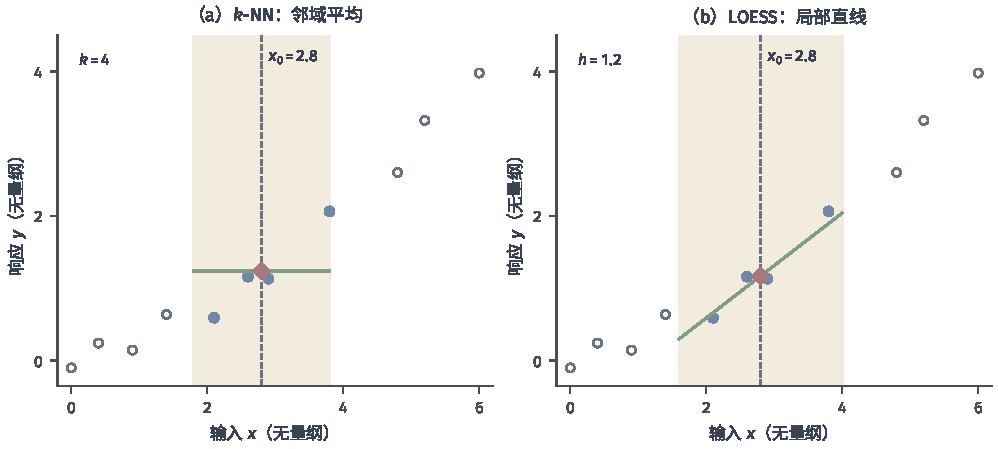
\includegraphics[width=159.059mm]{figures/03-models/01-classic-models/matplotlib/regression-neighborhood/figure.pdf}
  \caption{同一查询点上的邻域平均与局部线性拟合。横、纵轴均无量纲，所有点均为构造样本；空心点为未使用样本，蓝色实心点为本次使用的四个样本，菱形为$x_0=2.8$处的预测。左图取$k=4$、等权平均，预测约为$1.238$；右图取$h=1.2$与三立方距离权重，不做残差重加权，局部线性预测约为$1.171$。浅色带标出各自的邻域，两图同时改变了局部函数形式和权重，不据此断言某种方法总是更准。}
  \label{fig:regression-neighborhood}
\end{figure*}

\subsubsection{参数学习}

设局部基设计为$\bm{P}$，权重矩阵为$\bm{W}=\operatorname{diag}(K_i)$。若$\bm{P}^{\top}\bm{W}\bm{P}$可逆，便可解加权正规方程得到局部系数；实际使用$\bm{W}^{1/2}\bm{P}$的QR分解等方法更合适。邻域无样本或有效点不足以确定多项式时，应扩大邻域、降低阶数或明确回退规则，不能直接使用逆矩阵公式。

一维局部线性形式可写得更清楚。令$u_i=x_i-x_0$，$S_j=\sum_iK_iu_i^j$、$T_j=\sum_iK_iu_i^jy_i$，并记$\Delta=S_0S_2-S_1^2$。方程组为
\[
  \begin{pmatrix}S_0&S_1\\S_1&S_2\end{pmatrix}
  \begin{pmatrix}\widehat a\\\widehat b\end{pmatrix}
  =\begin{pmatrix}T_0\\T_1\end{pmatrix}.
\]
若$\Delta>0$，查询点上的截距可表示为
\begin{equation}
  \widehat m(x_0)=\sum_i l_i y_i,\qquad
  l_i=\frac{K_i(S_2-u_iS_1)}{\Delta}.
  \label{eq:regression-local-linear-weights}
\end{equation}
对非负核权重，$\Delta=\sum_{i<j}K_iK_j(u_i-u_j)^2$，所以至少需要两个不同输入具有正权重。即使$\Delta>0$，接近退化的设计也可能产生很大的$l_i$。

固定带宽与只依赖输入的权重时，估计是响应$\bm{y}$的线性函数。稳健LOESS则在初次拟合后根据残差增加降权系数，再重复局部拟合；权重一旦依赖响应，整体估计便不再是固定的线性平滑算子，下面的固定权重方差公式不能直接沿用。若一个查询使用$n_{\mathrm{loc}}$个有效样本、$q$个局部基函数，稠密拟合约需$O(n_{\mathrm{loc}}q^2+q^3)$运算，另加邻域查询成本。

\subsubsection{理论分析}
\label{sec:regression-loess-theory}

LOESS为每个查询点建立局部拟合，因此表示与计算都随邻域改变。固定输入和权重后，加权设计的秩决定系数能否唯一求出；在一维随机设计下，带宽又决定邻域逼近误差与响应平均的方差。下面把这两层分开，先用精确权重解释一次函数的再现，再在指定带宽序列下展开局部偏差与方差。

\paragraph{表达能力}
LOESS用每个查询点附近的低阶多项式描述局部趋势。带宽越宽，被同一个局部模型覆盖的输入越多，模型也越可能跨越规律的突变；阶数增加则能表达更高阶曲率，同时需要更多有效样本来确定系数。

\paragraph{收敛性}
固定查询点、带宽和邻域权重后，局部多项式拟合是加权最小二乘问题。加权设计满列秩时，求解线性系统即可得到唯一系数；秩亏时则需降阶、正则化或规定回退方式。若加入依赖残差的稳健重加权，外层权重也随拟合改变，单次加权最小二乘的可解性不再等于整个迭代必然收敛，仍需检查相应目标和停止准则。

\paragraph{泛化性}
局部线性拟合的核心收益是精确再现一次函数。由式\eqref{eq:regression-local-linear-weights}直接求和，
\[
  \sum_i l_i=1,\qquad \sum_i l_i u_i=0.
\]
因此当$m(x)=a+bx$时，$\sum_i l_i m(x_i)=m(x_0)$，不要求样本在$x_0$两侧对称。第二个恒等式解释了局部线性为何能消去一阶趋势造成的偏差。

最终权重$l_i$却不必非负。例如$x_0=0$、$x_1=0.1$、$x_2=0.2$、$K_1=K_2=1$时，$(l_1,l_2)=(2,-1)$。对构造响应$y_i=x_i$，局部线性预测为$0$，局部常数预测为$0.15$。若这两个响应分别加入独立方差为$\sigma^2$的噪声，两种预测的方差则为$5\sigma^2$与$\sigma^2/2$。消除线性偏差需要付出方差代价，不能直接推出局部线性总有更小风险。

更一般地，固定输入且误差条件独立、方差$v(x_i)\leq\sigma^2$时，
\[
  B_n=\sum_i l_i[m(x_i)-m(x_0)],\qquad
  V_n=\sum_i l_i^2v(x_i)
\]
分别为条件偏差和方差。若$m$在覆盖有效邻域的区间二阶连续可微且$|m''|\leq M_2$，用一次项抵消与Taylor余项可得
\[
  |B_n|\leq\frac{M_2}{2}\sum_i|l_i|u_i^2,\qquad
  V_n\leq\sigma^2\sum_i l_i^2.
\]
绝对值不能删去，也不能把这些权重当作凸组合套用$k$-NN回归误差界。

在内部点及规则随机设计下，上述精确公式可进一步化为熟悉的渐近偏差方差展开。局部多项式的系统分析见Fan与Gijbels的专著；下面明确给出本章使用的条件与推导\scite{fan1996local}。

以下余项随随机训练输入变化。记$Z_n=o_P(a_n)$表示$Z_n/a_n$依概率趋于零，$Z_n=O_P(a_n)$表示该比值依概率有界：对任意$\delta>0$，存在有限$M$使充分大的$n$满足$\mathbb{P}(|Z_n/a_n|>M)<\delta$。

\Needspace{16\baselineskip}
\begin{theorem}[一维内部点的局部线性展开]
  \label{thm:regression-local-asymptotic}
  设$(X_i,Y_i)$独立同分布，固定内部点$x_0$附近的输入密度$p$连续且$p(x_0)>0$，回归函数$m$二阶连续可微，条件方差$v$在$x_0$连续且有限。核$K$非负、有界、对称，支撑在$[-1,1]$，满足$\int K=1$和$\mu_2=\int u^2K(u)\,du>0$。取确定带宽$h\to0$、$nh\to\infty$，$K_i=K((X_i-x_0)/h)$，记$R(K)=\int K(u)^2du$。在可逆事件上，条件偏差与方差满足
  \begin{align*}
    B_n&=\tfrac12 m''(x_0)\mu_2h^2+o_P(h^2),\\
    V_n&=\frac{v(x_0)R(K)}{nhp(x_0)}+o_P((nh)^{-1}).
  \end{align*}
  可逆事件的概率趋于$1$；在退化事件上须另设估计值。
\end{theorem}

\begin{proof}
令$\mu_j=\int u^jK(u)\,du$。变量替换给出，对$j=0,1,2,3$，
\[
  \frac{\mathbb{E}S_j}{nh^{j+1}}
  =\int u^jK(u)p(x_0+hu)\,du\longrightarrow p(x_0)\mu_j.
\]
局部有界密度与有界紧支撑核给出$\operatorname{Var}(S_j/(nh^{j+1}))=O((nh)^{-1})$，故相应归一化矩依概率趋于$p(x_0)\mu_j$。由$\mu_1=\mu_3=0$，
\[
  \frac{\Delta}{n^2h^4}\xrightarrow{P}p(x_0)^2\mu_2>0,\qquad
  \sum_i l_i u_i^2
    =\frac{S_2^2-S_1S_3}{\Delta}
    =h^2\mu_2+o_P(h^2).
\]
此外$\sum_i|l_i|\leq S_0(S_2+h|S_1|)/\Delta=O_P(1)$。将$m(X_i)$在$x_0$处展开，常数与一次项分别由权重恒等式再现和抵消；二阶连续性使$|u_i|\leq h$内的余项一致为$o(h^2)$，于是得到偏差公式。

为求方差，令$A_j=\sum_iK_i^2v(X_i)u_i^j$，$j=0,1,2$。同样的均值与方差估计给出
\[
  \frac{A_j}{nh^{j+1}}
    \xrightarrow{P}p(x_0)v(x_0)\int u^jK(u)^2du.
\]
把权重公式代入精确条件方差，得到
\[
  V_n=\frac{S_2^2A_0-2S_2S_1A_1+S_1^2A_2}{\Delta^2}.
\]
分子第一项与分母的上述极限给出$v(x_0)R(K)/(nhp(x_0))$，含$S_1$的两项为较小阶，方差公式成立。
\end{proof}

当偏差和方差的领先系数都为正时，平衡$h^4$与$1/(nh)$提示$h$取$n^{-1/5}$量级，对应条件风险的$n^{-4/5}$尺度。若曲率为零，领先偏差项消失，不能仍按同一常数求最佳带宽。这些是随机设计下依概率成立的条件展开；改成无条件均方误差展开还需控制退化设计和余项的可积性。边界点的核矩被截断，也不能直接沿用内部点常数。

\subsubsection{支持局部常数（Nadaraya-Watson 核平滑）}
\label{sec:regression-nadaraya-watson}

在式\eqref{eq:regression-local-polynomial}中只拟合截距，对截距求导便得到\term{Nadaraya--Watson核平滑}（Nadaraya--Watson kernel smoothing）
\begin{equation}
  \widehat m_{\mathrm{NW}}(\bm{x}_0)
  =\frac{\sum_iK_i y_i}{\sum_iK_i},
  \qquad \sum_iK_i>0.
  \label{eq:regression-nw}
\end{equation}
它与局部多项式使用相同的邻域权重，但只作加权平均。Nadaraya与Watson分别研究了这一核回归路线；具体带宽和设计条件仍须与所用理论结果对应\scite{nadaraya1964,watson1964}。

在联合密度存在的设定下，$m(x)p(x)=\int y\,p(x,y)\,dy$，所以归一化核响应和可估计$m(x)p(x)$，核计数可估计$p(x)$，比值便近似条件均值。

局部常数权重和为$1$，但通常不满足一阶矩为零。因此一侧邻域的斜率可能带来一阶偏差。以一维内部点为例，把经验核和换为总体积分，记总体平滑值为$m_h(x_0)$。在$m,p$二阶连续可微、$p(x_0)>0$及前述对称紧支撑核条件下，对分子$\int K(u)m(x_0+hu)p(x_0+hu)\,du$和分母$\int K(u)p(x_0+hu)\,du$分别展开，得到
\[
  m_h(x_0)-m(x_0)
  =\mu_2h^2\left[\frac{m''(x_0)}{2}
       +\frac{m'(x_0)p'(x_0)}{p(x_0)}\right]+o(h^2).
\]
后一项反映设计密度不均匀的影响。局部线性消去这项并改善边界处的一阶偏差，但其负权重可能增大方差，所以选择仍应看总风险。

\subsubsection{小结}

LOESS用局部斜率或曲率补充局部平均，适合观察低维输入与响应之间的平滑关系。其有效性取决于局部数据量、设计秩、带宽和光滑程度；稳健重加权可以减轻部分异常响应影响，却没有消除所有异常点风险。局部曲线和导数描述特定输入附近的变化，可据此检查响应趋势；它们的解释随查询位置与带宽改变。

\subsection{模型对比与总结}

$k$-NN回归与LOESS都根据查询点选择局部数据，差别在于是否拟合邻域内的趋势。$k$-NN回归的均匀权重便于控制方差，局部线性权重能再现一次函数，却可能为负。比较风险时，需要同时计入设计位置、局部对称性和密度：这些条件会改变两者的偏差阶，也会改变方差的大小。

平滑样条沿另一条路线控制函数曲率，径向基函数网络则先选中心再学习全局展开系数。它们与邻域方法都使用局部性或相似性，但目标并不相同。尤其Nadaraya--Watson的系数由查询点归一化得到，核岭回归的训练系数则由整个Gram矩阵耦合求解；二者一般不等价。选择方法时应同时比较局部光滑性、输入的有效维数、权重如何学习以及查询预算。

\section{基于树与规则的回归}
\label{sec:regression-trees}

第\ref{sec:classic-overview-tree-rules}节已经给出条件分支与区域预测的共同结构。本节关注回归时怎样按响应损失选择区域，并确定叶内预测。CART采用递归划分，模型树在叶内加入线性趋势，MARS用连续铰链基表达阈值及交互。MARS的基函数可以重叠，并不构成标准决策树；把它放在这里，是为了比较不同的条件与分段表达。

\subsection{CART 回归树}
\label{sec:regression-cart}

\term{分类与回归树}（classification and regression trees, CART）将递归二分、叶内估计和复杂度剪枝组织成统一框架。Breiman等人在1984年的专著中系统阐述了这套方法，把数据决定的分区与树的规模控制联系起来。回归情形通常用平方误差评价分裂，再通过独立验证选择树的规模；这一流程将在下面分别展开\scite{breiman1984cart}。

第\ref{sec:classification-cart}节的分类CART共享递归二分与代价复杂度剪枝。任务差异落在分裂和叶输出上：本节按响应平方误差选择分区并输出叶均值，分类树按类别不纯度或误分类代价分裂，并输出类别标签或类别比例。

\subsubsection{模型结构}

设树$T$的叶区域为$R_1,\ldots,R_M$，则
\begin{equation}
  f_T(\bm{x})=\sum_{m=1}^{M}c_m\mathbf{1}\{\bm{x}\in R_m\}.
  \label{eq:regression-cart-model}
\end{equation}
数值特征上的节点规则通常为$x_j\leq s$与$x_j>s$，递归后形成轴对齐区域；类别特征则可按类别子集分支，不宜继续称为普通欧氏矩形。缺失值并非由树结构自动解决，还需指定缺失方向或其他规则。例如，\term{替代分裂}（surrogate split）在主测试特征缺失时，用其他特征的测试尽量复现主分裂的左右分配。

固定非空叶的样本索引集$I_m$后，令$\bar y_m=|I_m|^{-1}\sum_{i\in I_m}y_i$，有
\[
  \sum_{i\in I_m}(y_i-c)^2
  =\sum_{i\in I_m}(y_i-\bar y_m)^2+|I_m|(c-\bar y_m)^2.
\]
因此$c_m=\bar y_m$在平方损失下最优。改用绝对或分位数损失时，叶预测相应变为中位数或分位数；模型结构与损失选择仍然可以分开。

图\ref{fig:regression-tree-prediction}把一棵给定的阈值树展开为预测函数。沿树走到同一叶的输入共享一个预测值，所以一维常数叶回归树产生水平分段，而阈值处可以跳跃。图中每个叶的数值都来自该叶的两条响应，后面的学习问题才是如何从候选阈值中选出这些分区。

\begin{figure*}[t]
  \centering
  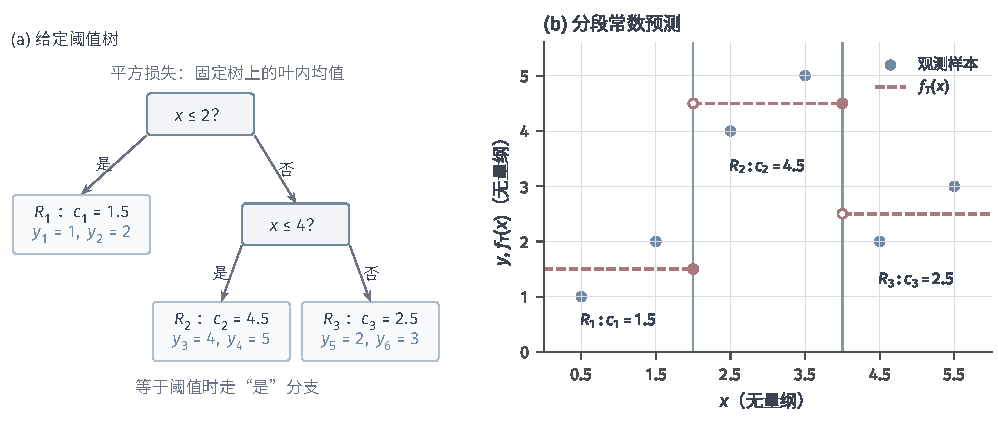
\includegraphics[width=159.059mm]{figures/03-models/01-classic-models/matplotlib/regression-tree-prediction/figure.pdf}
  \caption{给定阈值树与分段常数预测。六个无量纲教学样本按$x$递增排列；按$x\leq2$及右分支上的$x\leq4$划分后，三组响应分别为$(1,2)$、$(4,5)$、$(2,3)$，叶均值为$1.5$、$4.5$、$2.5$。蓝色点表示样本，红色虚线表示预测，绿色竖线表示阈值；阈值处实心、空心端点区分取与不取该值。右图只显示$0\leq x\leq6$，树结构预先给定。}
  \label{fig:regression-tree-prediction}
\end{figure*}

\subsubsection{参数学习}
\label{sec:regression-cart-learning}

在当前节点内，算法枚举特征与候选阈值，选择子节点平方误差和最小的分裂。对两个非空子节点，记样本数为$n_L,n_R$，均值为$\bar y_L,\bar y_R$，则分裂增益可精确写成
\begin{equation}
  \Delta_{\mathrm{split}}
  =\mathrm{SSE}_{\mathrm{parent}}
    -\mathrm{SSE}_{L}-\mathrm{SSE}_{R}
  =\frac{n_Ln_R}{n_L+n_R}(\bar y_L-\bar y_R)^2.
  \label{eq:regression-cart-gain}
\end{equation}
证明只需把两个子节点响应分别围绕自己的均值展开，再利用父均值为加权平均。该式说明增益同时考虑两组均值差异和样本量。

连续特征只需在相邻不同取值之间设候选切分，排好序后用累计和、平方和更新各侧SSE。类别子集有更多候选；在无额外分裂约束的平方误差二分问题中，可先按类别响应均值排序再考虑相邻分组，但带最小样本数、权重或其他限制时须重新检查相应结论。停止条件可限制最大深度、最小叶样本数和最低增益。贪心选择只保证当前节点在候选集中的最佳切分，不保证整棵树全局最优。

树生长后，用叶数惩罚控制规模。固定一个已生长的有限二叉树$T_0$，对其剪枝子树$T$定义
\begin{equation}
  R_\alpha(T)=\sum_{m\in\operatorname{leaves}(T)}
                    \mathrm{SSE}_m+\alpha|\operatorname{leaves}(T)|,
  \qquad\alpha\geq0.
  \label{eq:regression-pruning}
\end{equation}
\term{代价复杂度剪枝}（cost-complexity pruning）在保留局部拟合与减少叶数之间作折中。临界$\alpha$处可能出现多个最优子树，唯一性需要额外的并列规则。

\Needspace{11\baselineskip}
\begin{theorem}[固定生长树内的最优剪枝]
  \label{thm:regression-pruning}
  设$Q_\alpha(v)$为从$T_0$的节点$v$出发可得到的所有剪枝子树的最小代价。若$v$是原始叶，则$Q_\alpha(v)=\mathrm{SSE}_v+\alpha$；若$v$有左右孩子$v_L,v_R$，则
  \[
    Q_\alpha(v)=\min\{\mathrm{SSE}_v+\alpha,\,
                     Q_\alpha(v_L)+Q_\alpha(v_R)\}.
  \]
  从叶到根计算该递推，并保存每次选择，可得到$R_\alpha$的最优剪枝子树。
\end{theorem}

\begin{proof}
原始叶无其他选择，结论成立。对内部节点，任何合法剪枝子树要么把$v$收缩为一片叶，要么保留分裂。前者代价为$\mathrm{SSE}_v+\alpha$；后者的两个孩子可以独立剪枝，代价相加，归纳假设给出最小和为$Q_\alpha(v_L)+Q_\alpha(v_R)$。这两类穷尽全部选择，因此取最小值即可。相等时两个选择都最优，记录任一个并列规则均可返回一个最优解。
\end{proof}

固定$\alpha$时，递推只需对每个节点作常数次比较，因此在节点SSE已知后为$O(|T_0|)$。经典最弱环节方法进一步构造随$\alpha$变化的嵌套剪枝路径，再通过验证选择规模；它优化的仍是给定生长树内的剪枝集合，而不是所有可能的树。交叉验证时，各折的生长与剪枝都应仅使用该折训练集。

\subsubsection{理论分析}
\label{sec:regression-cart-theory}

回归树通过数据选择分区，再用叶内响应估计预测。叶区域和叶输出共同决定表示，分裂与剪枝决定搜索范围，响应同时参与这两个环节则影响统计误差。下面先说明有限训练集上的计算何时结束，再通过独立的结构样本与估计样本，展示可以直接证明的叶平均误差；普通CART的响应自适应性需要另行处理。

\paragraph{表达能力}
常数叶回归树为每个叶区域赋予一个预测值。增加叶数可以细化分区，但轴对齐切分若要逼近斜向或平滑关系，往往需要许多区域。有限叶数下的表示误差，因此同时受目标几何和分裂方式影响。

\paragraph{收敛性}
在有限训练集上，若每次分裂都产生两个非空子节点，叶数至多为$n$，树的生长会在有限步内终止。对固定生长树，前述剪枝递推也能在有限步内求得该树内的最优剪枝。这些计算性质没有把逐节点贪心搜索变成所有树结构上的全局优化，也没有回答样本量增加时的预测误差是否趋于零。

\paragraph{泛化性}
固定分区后的叶均值看起来类似$k$-NN回归的局部平均，但普通CART使用同一批响应选择分裂并估计均值。条件于最终分区，不会自动使被选中的噪声重新保持零均值。分析响应自适应分区需要控制分区类和选择过程，Nobel关于数据依赖分区的工作正是从这类条件出发；叶直径与样本数条件需要与分区选择的复杂度控制共同使用\scite{nobel1996partitions}。

用独立数据分别选分区和估计叶均值，可以得到一个透明的有限样本结论。\term{诚实分区}（honest partitioning）在这里指：结构样本决定分区，独立估计样本提供叶内被平均的响应。

\Needspace{14\baselineskip}
\begin{theorem}[独立分区下的叶平均误差]
  \label{thm:regression-honest-tree}
  用结构样本选定可测分区$\Pi$，用独立同分布的估计样本计算叶均值。假设估计样本满足零条件均值噪声、条件方差不超过$\sigma^2$，回归函数$m$为$L$-Lipschitz。固定查询点$\bm{x}$，其叶为$A$，其中估计样本数为$N_A$，叶内最大样本距离为$R_A$。条件于结构样本与全部估计输入的信息$\mathcal G$，在$N_A>0$时，
  \[
    \mathbb{E}[(\widehat m_\Pi(\bm{x})-m(\bm{x}))^2\mid\mathcal G]
    \leq L^2R_A^2+\frac{\sigma^2}{N_A}.
  \]
  若空叶预测规定为零，则$N_A=0$时的条件误差为$m(\bm{x})^2$。
\end{theorem}

\begin{proof}
条件于$\mathcal G$，分区与叶成员已固定，估计响应的噪声仍条件独立且均值为零。非空叶内误差拆为$m$值之差的平均与噪声平均；前者绝对值不超过$LR_A$，后者方差不超过$\sigma^2/N_A$，交叉项期望为零。空叶使用预定值零，误差直接为$m(\bm{x})^2$。
\end{proof}

在有界$m$下，若$R_A\to0$、$N_A\to\infty$依概率成立，可用与$k$-NN回归相同的有界偏差分解和噪声界得到点态均方一致性。空叶概率随之趋零。这里的样本数是独立估计样本中的叶成员数，结构样本上的最小叶样本约束并不自动保证它。

普通CART不能直接套用这一界。考虑固定输入$(1,2,3)$、查询点$2$，真实$m\equiv0$，三个响应独立等概率取$\pm1$。令树必须在$1.5$和$2.5$之间择一分裂，查询叶始终含两个样本。只要左邻或右邻与中间响应同号，最小SSE切分就选到同号二点叶，预测平方为$1$；该事件概率为$3/4$。两侧均异号时预测为零，故实际风险为$3/4$，大于机械套用$\sigma^2/N_A$得到的$1/2$。该反例否定的是独立平均公式的直接挪用，并不声称所有CART程序都不一致。

有限样本下，单棵树还可能对数据扰动敏感，贪心分裂也可能错过只有联合出现才有效的交互。后续的Bagging、随机森林和梯度提升通过多棵树组合改善某些误差来源，但组合对偏差或方差的影响仍取决于数据、成员依赖和训练设定。

\subsubsection{支持分段线性叶节点（模型树 M5）}
\label{sec:regression-model-tree}

如果每个区域内的价格趋势近似线性，用多片常数叶逼近可能需要很多切分。\term{模型树}（model tree）在叶内拟合线性模型$f_m(\bm{x})=b_m+\bm{w}_m^{\top}\bm{x}_{A_m}$，其中$A_m$为该叶使用的特征集。M5是这条路线的代表，用树选择适用区域，再用局部回归描述区域内部的趋势\scite{quinlan1992m5}。

局部样本少时，叶内设计可能秩亏，需要选择变量或正则化。父子节点预测的加权混合可以缓和估计跳跃，但两侧叶模型在共同边界上没有被强制相等，因此这种平滑处理不自动保证函数连续。叶模型也可改为GLM、岭或Lasso，不过分裂准则、参数估计与复杂度惩罚需要与新模型配套，不能只替换叶公式就沿用全部CART理论。

\subsubsection{小结}

CART把回归拆为选分区与叶内估计，阈值规则适合表达局部条件关系。它对输入单位缩放通常不如距离方法敏感，但候选分裂数量、缺失值规则与叶内样本量仍会影响结果。固定生长树内的剪枝可以精确优化，整体建树仍是贪心搜索；同一响应参与选树的自适应性也必须进入统计分析。

\subsection{多元自适应回归样条（MARS）}
\label{sec:regression-mars}

树的阈值选择能够适应数据，常数叶却在边界处跳跃。\term{多元自适应回归样条}（multivariate adaptive regression splines, MARS）把阈值写进连续的铰链基函数，再从数据中选择这些基函数及其乘积。Friedman在1991年提出这一方法，将自适应选择结点与样条展开结合。它在可加模型与树式区域表达之间提供了另一种选择：多个基函数可同时作用于同一输入，预测不再由唯一一片叶决定\scite{friedman1991mars}。

\subsubsection{模型结构}

对特征$x_j$与结点$t$，\term{铰链函数}（hinge function）为$(x_j-t)_+$与$(t-x_j)_+$，它们在结点一侧为零，另一侧线性变化。MARS写成
\begin{equation}
  f(\bm{x})=\beta_0+\sum_{m=1}^{M}\beta_m B_m(\bm{x}),
  \qquad
  B_m(\bm{x})=\prod_{l=1}^{q_m}
                 [s_{m,l}(x_{j_{m,l}}-t_{m,l})]_+,
  \label{eq:regression-mars}
\end{equation}
其中$s_{m,l}\in\{-1,1\}$，$q_m$为该基的因子数。通常限制最高交互阶数，并对同一乘积中重复使用变量设规则，避免无约束扩张。

单个铰链连续但在结点不可微；含两个不同变量的乘积如$(x_1-3)_+(5-x_2)_+$在激活区域是二次乘积，不再是整体分段线性函数。铰链和乘积都连续，所以有限线性组合连续，但可微性需要额外平滑构造。严格加性版本只允许单变量基，增加乘积则允许指定阶数内的交互。

\subsubsection{参数学习}

前向阶段从常数模型开始，在当前基函数$B_l$、候选变量$j$与候选结点$t$中搜索，将$B_l(\bm{x})(x_j-t)_+$和$B_l(\bm{x})(t-x_j)_+$成对加入，并重新拟合线性系数。选择使训练平方误差下降最多的候选，直到达到基数、交互阶数或改善量限制。结点与基函数都由响应参与选择，因此整个训练过程不同于固定设计的一次OLS。

后向阶段逐个尝试删除非截距基函数，每次保留训练误差增加最小的删除，构造不同规模的模型序列。再从序列中按验证误差或广义交叉验证选模型，而不是一看到GCV不再下降就必然停止搜索。常用准则写成
\begin{equation}
  \operatorname{GCV}
  =\frac{\mathrm{SSE}/n}{(1-C_{\mathrm{eff}}/n)^2},
  \qquad C_{\mathrm{eff}}<n.
  \label{eq:regression-mars-gcv}
\end{equation}
$C_{\mathrm{eff}}$是复杂度计数，既考虑保留的线性系数，也以附加惩罚近似结点搜索的代价。例如可写成$q+cK$，其中$q$是保留设计的秩，$K$是采用相应计数约定的结点数，$c$是每个结点的附加代价。软件对成对基、交互结点与自由度有不同计数方式，使用GCV前需要明确采用哪种复杂度计数；该计数近似了搜索代价，区别于自适应拟合的精确自由度。

\subsubsection{理论分析}

MARS的表达来自铰链基及其乘积，训练则同时选择基函数和线性系数。固定基时可以精确求解最小二乘，前向与后向搜索只逐步改变当前基集合。统计分析还要包含响应参与选择所产生的误差，因此固定样条空间的结果与数据自适应搜索的结果，需要按各自条件使用。

\paragraph{表达能力}
MARS把目标展开为铰链基与其乘积的线性组合。结点数、基数量和交互阶数限定可选择的变化；提高交互阶数可以加入更多多变量关系，也增加候选搜索和系数估计的负担。

\paragraph{收敛性}
固定基函数后，系数可通过最小二乘求解。前向搜索在给定基数量上限或满足停止准则时结束，后向阶段每步删除基函数，也会在有限步内终止。前向与后向步骤都没有搜索全部可能基集合，因此不能由每一步的局部改善推出全局最优。

\paragraph{泛化性}
如果基函数由同一批响应选择，直接条件于所选设计再套用固定设计OLS的无偏性，就忽略了选择偏差。统计分析需要同时考虑系数估计与基函数选择。

样条与低阶交互函数空间有成熟的逼近和统计理论。例如，扩展线性建模研究了多项式样条及张量积表示怎样适应指定的低阶结构。这类结论对应指定的空间增长、平滑性和模型选择条件；评价具体MARS贪心实现时，还需验证其搜索和选择规则是否满足这些条件\scite{stone1997splines}。

MARS输出连续函数并不意味着其估计方差必小于CART。结点选择可以对样本扰动敏感，多个铰链也可能高度相关。实践中可限制交互阶数和基数量，并用独立验证比较预测；对数据范围外的外推尤其应检查，铰链的线性增长可能在缺少观测支持处产生较大的预测值。

\subsubsection{小结}

MARS通过自适应结点与铰链乘积表达阈值和交互，在线性系数层面仍可使用最小二乘。其连续性来自基函数，灵活性来自基选择；这两者分别对应表示与搜索问题。限制交互能减少候选复杂度，也可能遗漏真实关系，是否合适应由任务和数据判断。

\subsection{模型对比与总结}

CART用不重叠叶区域和常数预测，模型树在叶内增加线性趋势，MARS用可重叠的连续基函数及其乘积。前两者沿树路径路由，MARS需要计算保留的基；叶线性模型可能在边界跳跃，MARS的基本铰链构造则连续但不必处处可微。三者都允许阈值由数据决定，却使用不同的复杂度控制。

相关工作还从选择偏差和集成方式改进树模型。\term{条件推断树}（conditional inference tree）把变量关联检验与分裂位置选择分开，缓解候选切分多的变量更容易被选中的偏向；检验规则和显著性水平共同控制树大小，预测误差仍需由样本外评价确定\scite{hothorn2006ctree}。

\section{基于概率的回归}
\label{sec:regression-probabilistic}

一个房价点预测没有说明价格自身的波动，也没有说明有限数据下函数估计的差异。GLM已经通过条件分布描述前一种变化；本节进一步给未知系数或函数设置先验，由观测形成后验，再将函数不确定性与响应噪声一起带入预测分布。第\ref{sec:classic-overview-probabilistic}节的概率表示由此落实为可以计算的后验更新。

\term{分布回归}（distributional regression）提供了完整条件分布的另一条入口：先选择响应分布族，再让位置、尺度或形状等多个分布参数分别依赖输入。GAMLSS允许用线性项或平滑项建模这些参数，因而能表达均值不变但条件方差、偏度或尾部随输入变化的情形\scite{rigby2005gamlss}。它与只拟合若干分位点不同，也不等同于描述未知函数后验的GPR；代价是必须选择分布族、链接与各参数的结构，并用适当评分和校准诊断检查整个预测分布。

\subsection{高斯过程回归（GPR）}
\label{sec:regression-gpr}

对一组房屋属性，我们希望同时描述多个输入位置上的价格函数值及其相互关系。\term{高斯过程回归}（Gaussian process regression, GPR）用均值函数规定各位置的先验中心，用协方差函数规定函数值怎样共同变化。任意有限输入集合上的函数值都具有联合高斯分布，加入高斯观测噪声以后，可以精确计算后验与预测分布。先从有限权重模型推导这一计算，再转向函数值本身，就能看清它与贝叶斯线性回归、核岭回归的联系。

高斯过程预测较早已用于时间序列和地统计学，空间预测中的相关方法通常称为克里金（kriging）。20世纪90年代，Williams与Rasmussen在机器学习语境中讨论了GPR及协方差函数参数的学习，并将它与贝叶斯神经网络联系起来\scite{rasmussen2006}。

\subsubsection{模型结构}
\label{sec:regression-gpr-structure}

先考虑有限维特征$\bm{\phi}(\bm{x})\in\mathbb{R}^{p}$，令$f(\bm{x})=\bm{\phi}(\bm{x})^{\top}\bm{w}$。与OLS把$\bm{w}$看作待估计固定量不同，\term{贝叶斯线性回归}（Bayesian linear regression）对$\bm{w}$设置分布，再根据数据更新。使用高斯先验与高斯噪声，更新可通过完成平方得到。

\Needspace{14\baselineskip}
\begin{theorem}[贝叶斯线性回归的后验与预测]
  \label{thm:regression-bayesian-linear}
  条件于设计矩阵$\bm{X}$，设$\bm{w}\sim\mathcal{N}(\bm{m}_0,\bm{V}_0)$，其中$\bm{V}_0\succ0$，并设$\bm{y}=\bm{X}\bm{w}+\bm{\varepsilon}$，$\bm{\varepsilon}\sim\mathcal{N}(\bm{0},\sigma^2\bm{I})$与$\bm{w}$独立，$\sigma^2>0$。则
  \[
    \begin{aligned}
      \bm{V}_n&=(\bm{V}_0^{-1}+\sigma^{-2}\bm{X}^{\top}\bm{X})^{-1},\\
      \bm{m}_n&=\bm{V}_n
          (\bm{V}_0^{-1}\bm{m}_0+\sigma^{-2}\bm{X}^{\top}\bm{y}),
    \end{aligned}
  \]
  且$\bm{w}\mid\bm{X},\bm{y}\sim\mathcal{N}(\bm{m}_n,\bm{V}_n)$。新响应采用独立同方差噪声时，
  \[
    Y_{\star}\mid\bm{x}_{\star},\bm{X},\bm{y}
    \sim\mathcal{N}\bigl(
      \bm{\phi}_{\star}^{\top}\bm{m}_n,\,
      \bm{\phi}_{\star}^{\top}\bm{V}_n\bm{\phi}_{\star}+\sigma^2\bigr).
  \]
\end{theorem}

\begin{proof}
先验与似然的负对数相加，去掉与$\bm{w}$无关的项后为
\[
  \tfrac12\bm{w}^{\top}
       (\bm{V}_0^{-1}+\sigma^{-2}\bm{X}^{\top}\bm{X})\bm{w}
  -\bm{w}^{\top}
       (\bm{V}_0^{-1}\bm{m}_0+\sigma^{-2}\bm{X}^{\top}\bm{y}).
\]
定义定理中的$\bm{V}_n,\bm{m}_n$，上式等于
$\tfrac12(\bm{w}-\bm{m}_n)^{\top}\bm{V}_n^{-1}(\bm{w}-\bm{m}_n)$加常数。精度矩阵正定，故该可积密度归一化后就是所述高斯后验。新响应为后验高斯参数的线性变换与独立高斯噪声之和，均值与方差相加即得预测分布。
\end{proof}

若只需用一个参数向量概括后验，可取当前参数化下的后验众数，即最大后验估计（MAP）。固定设计与超参数，且最大值能够取到时，当前回归模型的目标为
\begin{equation}
  \begin{aligned}
    \widehat{\bm{w}}_{\mathrm{MAP}}
      &\in\argmax_{\bm{w}}p(\bm{w}\mid\bm{X},\bm{y})\\
      &=\argmax_{\bm{w}}
        \{\log p(\bm{y}\mid\bm{X},\bm{w})+\log p(\bm{w})\}.
  \end{aligned}
  \label{eq:regression-map}
\end{equation}
后验的归一化常数与$\bm{w}$无关，因而不影响最大化。MAP使用后验众数，后验均值则对参数按后验加权平均，两者一般不同（参考\BookSectionRef{sec:statistics-bayes-hierarchy}{第一卷“数学准备”的“有限维目标的估计”小节}）。

图~\ref{fig:regression-mle-map-geometry}在二维参数平面上展示这两个目标的差别。似然单独把最优点放在数据偏好的中心；零均值先验则偏好靠近原点的参数。MAP最小化负对数似然与负对数先验之和，因此落在二者共同决定的位置，而不是在MLE与先验中心之间任意作线性插值。椭圆形状和先验尺度改变时，折中的方向也会改变。
\begin{figure}[htbp]
  \centering
  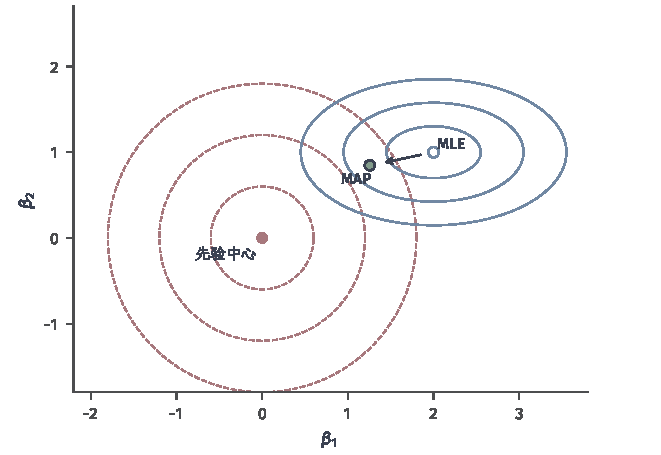
\includegraphics[width=105.412mm]{figures/03-models/01-classic-models/matplotlib/regression-mle-map-geometry/figure.pdf}
  \caption{MLE与MAP的参数几何。蓝色实线是以$(2,1)^\top$为中心、两坐标尺度分别为$1$和$0.55$的高斯似然等高线；红色虚线是以原点为中心、尺度为$1.3$的各向同性高斯先验等高线。空心点为MLE，绿色实心点为两项相加后的MAP $(1.256,0.848)^\top$。该构造用于显示先验如何改变点估计，不代表MAP总在两中心的连线上。}
  \label{fig:regression-mle-map-geometry}
\end{figure}

若$\bm{m}_0=\bm{0}$、$\bm{V}_0=\tau^2\bm{I}$，后验均值为$(\bm{X}^{\top}\bm{X}+\sigma^2\bm{I}/\tau^2)^{-1}\bm{X}^{\top}\bm{y}$，在本章归一化下对应$\lambda=\sigma^2/(n\tau^2)$的岭估计。高斯后验的均值与众数相同，所以也等于MAP估计。该对应要求截距处理一致：若先验惩罚全部特征系数，就不能直接与截距不受惩罚的岭模型比较。后验协方差与前面固定真参数下岭估计的重复抽样协方差也是不同对象。

有限维贝叶斯线性模型已经诱导出函数上的高斯分布：
\[
  m_0(\bm{x})=\bm{\phi}(\bm{x})^{\top}\bm{m}_0,\qquad
  k(\bm{x},\bm{x}')=\bm{\phi}(\bm{x})^{\top}\bm{V}_0\bm{\phi}(\bm{x}').
\]
任意有限个函数值都是高斯参数的线性变换，因此联合高斯。直接指定$m_0$和正定核$k$，便可越过显式系数建立函数先验。

\Needspace{6\baselineskip}
把这些相容的有限维高斯分布记为$f\sim\mathcal{GP}(m_0,k)$：任意有限输入集合上的函数值向量联合高斯。
正定核保证有限协方差矩阵半正定，扩张定理据此建立过程；连续样本路径的版本是否存在，还需额外的路径条件（参考\BookSectionRef{sec:rv-finite-dimensional-laws}{第一卷“数学准备”的“基于有限维分布的过程表示”小节}与\BookSectionRef{sec:rv-gaussian-generation}{第一卷“数学准备”的“基于高斯规律的随机过程生成”小节}）。

高斯过程允许有限秩核，因此并不必然对应无限维特征；有限维贝叶斯线性回归正是其中一个特例。对无限维核，也不需要先假设存在协方差为无限维单位矩阵的普通高斯权重向量，定义有限函数值的相容联合分布即可。

加入与函数独立的噪声$y_i=f(\bm{x}_i)+\varepsilon_i$，其中$\varepsilon_i$相互独立且服从$\mathcal{N}(0,\sigma^2)$，$\sigma^2>0$。令$\bm{K}_{i,j}=k(\bm{x}_i,\bm{x}_j)$，$(\bm{k}_{\star})_i=k(\bm{x}_i,\bm{x}_{\star})$，$\bm{m}_0$表示训练点上的先验均值向量，$\bm{C}=\bm{K}+\sigma^2\bm{I}$，$f_{\star}=f(\bm{x}_{\star})$。联合分布为
\[
  \begin{pmatrix}\bm{y}\\f_{\star}\end{pmatrix}
  \sim\mathcal{N}\!\left[
    \begin{pmatrix}\bm{m}_0\\m_0(\bm{x}_{\star})\end{pmatrix},
    \begin{pmatrix}
      \bm{C}&\bm{k}_{\star}\\
      \bm{k}_{\star}^{\top}&k(\bm{x}_{\star},\bm{x}_{\star})
    \end{pmatrix}\right].
\]
于是后验预测可以精确写成
\begin{equation}
  \begin{aligned}
    \mu_{\star}
      &=m_0(\bm{x}_{\star})
        +\bm{k}_{\star}^{\top}\bm{C}^{-1}(\bm{y}-\bm{m}_0),\\
    v_{\star}
      &=k(\bm{x}_{\star},\bm{x}_{\star})
        -\bm{k}_{\star}^{\top}\bm{C}^{-1}\bm{k}_{\star}.
  \end{aligned}
  \label{eq:regression-gp-posterior}
\end{equation}
为证明它，令$Z=f_{\star}-m_0(\bm{x}_{\star})-\bm{k}_{\star}^{\top}\bm{C}^{-1}(\bm{y}-\bm{m}_0)$。直接计算得到$\operatorname{Cov}(Z,\bm{y})=\bm{0}$；$Z$与$\bm{y}$联合高斯，所以独立。其方差为$v_{\star}$，从而条件于$\bm{y}$时，$f_{\star}$的均值为$\mu_{\star}$、方差为$v_{\star}$。该方差非负也由它是随机变量方差得到。未来带噪声响应的方差则为$v_{\star}+\sigma^2$。

核选择规定了先验中的相似性。平方指数核$k(\bm{x},\bm{x}')=\sigma_f^2\exp(-\lVert\bm{x}-\bm{x}'\rVert_2^2/(2\ell^2))$具有很强的平滑性，其中$\sigma_f^2>0$是信号方差、$\ell>0$是长度尺度。Matérn核可调节平滑程度，例如$\nu=3/2$时为$\sigma_f^2(1+\sqrt3r/\ell)\exp(-\sqrt3r/\ell)$，其中$r=\lVert\bm{x}-\bm{x}'\rVert_2$，对应一次均方可微的过程。一维周期核可写成$\sigma_f^2\exp(-2\sin^2(\pi(x-x')/p)/\ell^2)$，表达周期$p>0$的相关结构。合法核的和与乘积仍合法，可以组合趋势与周期，但不保证所组合的结构符合实际数据。

图\ref{fig:regression-gp-posterior}展示了式\eqref{eq:regression-gp-posterior}的两项输出。在这个固定平稳核的例子中，观测附近的函数值受到较强约束，观测间的较大空隙与远离观测的区域保留更多不确定性。曲线给出点预测，带状区域则说明在当前先验和噪声设定下，哪些函数值仍与数据相容。

\begin{figure}[htbp]
  \centering
  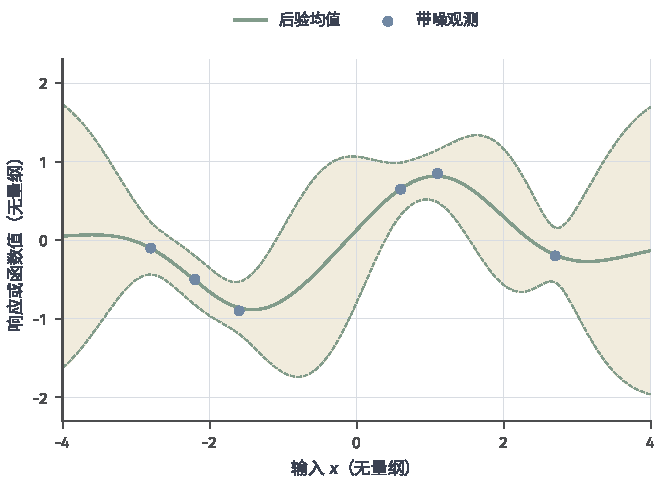
\includegraphics[width=105.412mm]{figures/03-models/01-classic-models/matplotlib/regression-gp-posterior/figure.pdf}
  \caption{高斯过程的后验均值与函数不确定性。六个点为构造观测；先验均值为零，平方指数核取$\ell=0.9$、$\sigma_f=1$，观测噪声标准差为$\sigma=0.18$。实线为$\mu_{\star}$，浅色带及虚线边界为$\mu_{\star}\pm1.96\sqrt{v_{\star}}$，表示潜在函数值的逐点约$95\%$后验可信区间。它不是整条函数的同时可信带；预测未来带噪响应时，方差还须加$\sigma^2$。}
  \label{fig:regression-gp-posterior}
\end{figure}

\subsubsection{参数学习}
\label{sec:regression-gpr-learning}

给定核和噪声参数时，后验已经由式\eqref{eq:regression-gp-posterior}确定；仍需选择长度尺度、信号方差、噪声方差及可能的均值参数。令这些超参数为$\bm{\theta}$，把训练输入处的潜在函数值积分掉，得到\term{边缘似然}（marginal likelihood）：在给定输入和超参数时，观测响应向量的概率密度。以下令先验均值为零：
\begin{equation}
  \log p(\bm{y}\mid\bm{X},\bm{\theta})
   =-\tfrac12\bm{y}^{\top}\bm{C}_{\bm{\theta}}^{-1}\bm{y}
    -\tfrac12\log|\bm{C}_{\bm{\theta}}|
    -\tfrac n2\log(2\pi).
  \label{eq:regression-gp-evidence}
\end{equation}
二次项评价响应与协方差结构的匹配，行列式项来自密度归一化，两者共同决定目标。行列式随核的尺度和相关结构变化，外层优化据此选择当前核族中的超参数；所选结构的预测效果仍需用样本外数据检查。

若$\bm{a}=\bm{C}^{-1}\bm{y}$，固定零均值模型的梯度为
\[
  \frac{\partial\log p(\bm{y})}{\partial\theta_j}
  =\tfrac12\operatorname{tr}\!\left[
    (\bm{a}\bm{a}^{\top}-\bm{C}^{-1})
    \frac{\partial\bm{C}}{\partial\theta_j}\right].
\]
它来自$d\bm{C}^{-1}=-\bm{C}^{-1}(d\bm{C})\bm{C}^{-1}$与$d\log|\bm{C}|=\operatorname{tr}(\bm{C}^{-1}d\bm{C})$。可以在正参数的对数坐标上使用梯度算法，多初值比较有助于发现不同局部最优；这种经验贝叶斯拟合通常仍把所选超参数当作固定值，因此没有保留全部超参数不确定性。

数值计算使用Cholesky分解$\bm{C}=\bm{L}\bm{L}^{\top}$。解两次三角方程得到$\bm{a}$后，预测均值为$\bm{k}_{\star}^{\top}\bm{a}$；令$\bm{v}=\bm{L}^{-1}\bm{k}_{\star}$，预测方差为$k(\bm{x}_{\star},\bm{x}_{\star})-\lVert\bm{v}\rVert_2^2$。稠密分解需要$O(n^3)$时间、$O(n^2)$存储，预计算后的单点均值需$O(n)$算术加核计算，单点方差通常需$O(n^2)$三角求解。均值与方差不能统称同一个预测代价。

大数据下可选取$m\ll n$个输入位置$\bm{z}_j$，以潜在函数值$u_j=f(\bm{z}_j)$作为\term{诱导变量}（inducing variables），通过它们的近似后验概括数据对函数的约束。Titsias的变分诱导点方法在高斯回归中优化边缘对数似然的变分下界，以选择诱导输入并近似后验，常见稠密计算规模为$O(nm^2)$；后续随机变分方法进一步支持小批量训练。近似是否充分，仍需检查诱导表示能否保留任务所需的函数变化\scite{titsias2009}。

\subsubsection{理论分析}
\label{sec:regression-gpr-theory}

GPR的核规定未知函数怎样变化，训练观测通过高斯条件分布更新这些函数值。固定核和正噪声方差时，这一步是正定线性系统求解；继续学习核超参数时，外层目标则可能非凸。样本增加后的后验集中属于另一个统计问题，需要明确抽样制度、真函数光滑性与先验尺度，区间覆盖也要按相应模型和超参数处理评价。

\paragraph{表达能力}
GPR的核规定函数变化的先验结构和平滑尺度，后验均值用训练点处的核函数组合预测。核尺度过大可能压平目标中的局部变化，观测范围不足则使部分输入上的后验主要受先验影响。核与噪声设定还共同决定后验区间，因此精确条件计算的意义始终依赖这些表示假设。

\paragraph{收敛性}
固定核超参数与正噪声方差后，精确GPR通过正定线性系统求解后验，其计算误差来自线性系统的数值求解。若用迭代线性求解器替代矩阵分解，其收敛仍取决于矩阵条件数和算法；外层核超参数优化则可能是非凸的，不能沿用内部线性求解的保证。

后验均值还能解释为正则化核回归的最优解。为建立这一联系，回顾第\ref{sec:classic-overview-kernel-validity}节的再生核Hilbert空间（RKHS）：记核$k$对应的函数空间为$\mathcal H_k$，其核截面满足$f(\bm{x})=\langle f,k(\bm{x},\cdot)\rangle_{\mathcal H_k}$。这一再生关系把函数取值化为内积，也使核范数可以作为函数复杂度惩罚。

数据拟合项只依赖训练点上的有限个函数值。严格递增的范数惩罚会排除这些取值无法识别的正交分量；在最优解存在且最优值有限时，最优函数可限制到训练点核截面的张成空间（参考\BookTheoremRef{thm:functional-representer-theorem}{第一卷“数学准备”的有限样本表示定理}）。

对给定正定核$k$与$\lambda>0$，考虑本章归一化下的核岭回归目标
\[
 \min_{f\in\mathcal H_k}
 \frac1{2n}\sum_i(y_i-f(\bm x_i))^2
 +\frac{\lambda}{2}\lVert f\rVert_{\mathcal H_k}^2.
\]
这个平方损失目标可以直接构造最优函数。令$\bm K_{i,j}=k(\bm x_i,\bm x_j)$，$(\bm k_{\bm x})_i=k(\bm x_i,\bm x)$，其唯一函数解为
\[
 \widehat f(\bm x)=\bm k_{\bm x}^\top\bm\alpha_0,\qquad
 \bm\alpha_0=(\bm K+n\lambda\bm I)^{-1}\bm y.
\]
在有限核表示中，系数满足$\bm K[(\bm K+n\lambda\bm I)\bm\alpha-\bm y]=\bm0$。由于$\bm K$半正定且$\lambda>0$，移位矩阵正定，解$\bm\alpha_0$存在并满足驻点条件；系数目标凸，因此该解达到最小值。正系数的范数平方项使函数目标严格凸，所以函数解唯一；核矩阵奇异时，给系数加上$\ker\bm K$中的向量仍表示同一函数，表示系数则可能不唯一（求解步骤参考\BookSectionRef{sec:functional-finite-parameter-solvers}{第一卷“数学准备”的“基于有限表示的参数求解”小节}）。

将$\lambda=\sigma^2/n$代入该解，与式\eqref{eq:regression-gp-posterior}的零均值后验预测完全一致。非零先验均值时，应对$\bm{y}-\bm{m}_0$做相同核岭拟合，再加回$m_0(\bm{x})$。等价关系要求核尺度、均值和截距处理一致；若某个模型额外加入不受惩罚的截距，其解通常需要另解增广系统。

\paragraph{泛化性}
点预测相同以后，推断仍需明确要评价哪一种不确定性。GP方差是模型内潜在函数的后验不确定性，KRR目标本身只确定一个函数估计；后者也可以配合频率学理论或校准构造区间。固定核超参数时，GP后验方差只依赖输入与噪声设定，不直接依赖观测响应；输入间的相关性由核决定，不能简单归纳为“欧氏距离越远方差必然越大”。高斯可信区间在先验模型下有后验概率解释，模型失配或超参数估计后不自动具有同样的重复抽样覆盖率。

后验收缩研究样本增加时后验质量是否集中到真实函数附近。已有理论把收缩速度与先验函数落入小半径范数球的概率、真函数相对于RKHS的可逼近性及先验尺度联系起来。前一种概率称为小球概率，它衡量先验在局部函数邻域内分配了多少质量；固定设计与随机设计的结论还需分别说明所使用的函数距离\scite{vaart2008gp}。

例如，在$\alpha>0$阶光滑函数的非参数回归比较中，常见的$L^2$误差尺度为$n^{-\alpha/(2\alpha+d)}$，其平方尺度则为$n^{-2\alpha/(2\alpha+d)}$。某个GP先验能否达到这样的尺度，还取决于平滑度与先验尺度的匹配，以及具体观测设定和距离。后验收缩本身也不自动给出后验均值风险界或可信区间的频率覆盖保证。

\subsubsection{支持非高斯似然（拉普拉斯近似与期望传播）}
\label{sec:regression-gp-nongaussian}

计数或二分类响应需要不同似然。仍可设潜在函数服从GP，借助$\exp(f)$或logistic函数映射到条件均值，但$p(\bm{f}\mid\bm{y})\propto p(\bm{y}\mid\bm{f})p(\bm{f})$一般不再是高斯，不能继续使用精确高斯回归公式。

\term{拉普拉斯近似}（Laplace approximation）在后验众数$\widehat{\bm{f}}$附近用二阶Taylor展开近似对数密度。若零均值先验的$\bm{K}$正定，并在众数处定义$\bm{W}=-\nabla^2\log p(\bm{y}\mid\bm{f})$，后验局部高斯近似为
\[
  q(\bm{f})=\mathcal{N}\bigl(
       \widehat{\bm{f}},(\bm{K}^{-1}+\bm{W})^{-1}\bigr),
\]
前提是该精度矩阵正定。若核有限秩，需在其有效子空间中计算；不能直接写不存在的$\bm{K}^{-1}$。多峰或强偏斜后验可能无法由一个局部高斯充分描述。

\term{期望传播}（expectation propagation, EP）用便于处理的近似因子替代逐个似然因子，在移除当前近似因子后形成的分布上加入真实因子，再匹配相应矩。它与拉普拉斯近似使用不同的局部信息，不保证对所有问题都更准确或必然收敛。变分推断则通过优化分布族中的近似准则处理后验，并可结合诱导变量。无论采用哪一种近似，最终的观测预测仍需积分$p(y_{\star}\mid f_{\star})$；潜在高斯的均值方差并不意味着观测响应也服从高斯\scite{rasmussen2006}。

\subsubsection{小结}

GPR用核规定函数先验，在高斯噪声下精确更新任意有限查询集合的分布。有限维贝叶斯线性模型、非线性核和非高斯似然都可在这一思路中理解，但核选择、超参数估计与近似推断分别引入新的条件。计算瓶颈主要来自训练协方差矩阵；只需点预测与还需完整方差时，计算预算并不相同。

第\ref{sec:dim-gplvm}节的GPLVM复用GP核协方差和边缘似然计算，却把低维输入坐标也作为未知量：GPR从已观测输入预测数值响应，GPLVM则从高维观测反求低维坐标并学习由低维空间到观测空间的映射。二者共享概率函数表示，不共享任务方向与待估计对象。

\subsection{模型对比与总结}

贝叶斯线性回归与GPR的共同点是对函数不确定性进行更新，区别主要在于表示方式与计算所依赖的规模变量。有限特征模型也可以通过非线性基表示曲线；GP也可以使用有限秩核，因此不能把两者简单分成“只能线性”和“必然无限维”。若显式基维数为$p$，贝叶斯线性回归的稠密训练通常需$O(np^2+p^3)$运算，而一般稠密GP主要受$n$控制；低秩表示可以在两种计算形式之间转换。

模型内后验区间在给定似然、先验和超参数处理下具有后验概率含义。分布无关覆盖方法则先固定已训练回归器及其评分规则，再用与训练分离的校准样本设定预测范围。条件于训练资料与训练随机性后，若校准样本与未来测试样本可交换，同一固定评分的共形秩构造可给出边际覆盖保证；这里的概率同时平均校准集与未来样本。分割共形预测可以校准点预测的残差；共形分位数回归（conformalized quantile regression, CQR）则保留已拟合的有序上下分位点随输入变化的形状，再用留出分数修正边际覆盖（参考\BookSectionRef{sec:reliability-guarantee}{第二卷“基础、理论和可信性”的“可靠性”章“可靠性的保证”节}）\scite{angelopoulos2022conformal,romano2019cqr}。这种覆盖保证允许基础回归器失配，但拟合质量会影响预测范围的宽度。比较区间还需同时报告覆盖与宽度。

贝叶斯方法还能与其他模型结合。\term{贝叶斯加性回归树}（Bayesian additive regression trees, BART）对树之和及叶参数设置正则化先验，使用后验采样获得函数和预测分布，连接了本章的树路线与概率路线\scite{chipman2010bart}。

贝叶斯神经网络对网络权重设置先验；在特定独立权重先验、尺度和无限宽极限下，某些网络诱导的函数分布趋于GP，并非任意网络结构或训练过程都具有这种极限。狄利克雷过程混合回归则对混合分布采用非参数先验，允许有效成分随数据变化；其优势在于表达多模态条件分布，成分解释与可识别性仍需检查。概率模型为决策提供分布信息，同时需要承担分布设定、后验计算与校准的成本。

\section{基于集成的回归}
\label{sec:regression-ensemble}

第\ref{sec:classic-overview-ensemble}节已给出Bagging、Boosting和Stacking的基本动机，第\ref{chap:ensemble-learning}章进一步说明成员怎样生成、依赖与组合。用于回归时，需要确定成员输出及组合后的预测对象：随机森林通常平均按平方损失训练的树预测；梯度提升的目标由所选回归损失决定；Stacking则由元学习器按回归目标组合成员预测。平均条件均值预测仍输出条件均值的估计；若任务要求分位数或覆盖区间，需要改变训练、聚合或校准规则。

比较树集成时，树深、树数、特征抽样、学习率和早停都应在训练流程中选择。袋外误差可以辅助诊断，仍不能替代最终测试；组合后也不能直接移植单棵树的剪枝最优性或独立叶平均证明。
分类投票的错误变化取决于成员错误的依赖，平均得分的方差变化取决于成员间的协方差；二分类AdaBoost则在各轮取得带权优势时控制训练误差上界，并结合投票类的容量或间隔分析总体风险（参考\BookSectionRef{sec:boosting}{第二卷“基础、理论和可信性”的“二分类学习的可学习性”章“集成学习”节}）。第\ref{sec:ensemble-quality-dependence-diversity}节讨论成员质量和错误依赖。实际选型应按表\ref{tab:regression-evaluation-protocol}中的预测对象比较误差、分布质量或区间覆盖，并同时记录训练与查询成本。

\section{模型选择与评价}
\label{sec:regression-evaluation}

\subsection{方法比较}

回归方法可能估计条件均值、指定分位数或完整分布。表\ref{tab:regression-navigation}把预测对象与函数表示、训练准则和区间解释放在一起比较；改变损失或概率设定，同一表示也可以服务于不同目标。

\begin{table*}[htbp]
  \centering
  \small
  \begin{tabularx}{\linewidth}{@{}>{\RaggedRight\arraybackslash}p{25mm}>{\RaggedRight\arraybackslash}X>{\RaggedRight\arraybackslash}X>{\RaggedRight\arraybackslash}X>{\RaggedRight\arraybackslash}X@{}}
    \toprule
    代表方法 & 预测对象 & 函数表示 & 训练准则 & 推断或校准 \\
    \midrule
    OLS & 条件均值 & 固定线性特征映射 & 平方损失 & 模型假设下的参数与预测区间 \\
    岭、Lasso & 条件均值的受约束逼近 & 固定线性特征映射 & 平方损失加$\ell_2$或$\ell_1$系数惩罚 & 不自动给出区间，需另加推断模型 \\
    分位数回归 & 指定条件分位数 & 线性特征映射 & 分位数损失 & 抽样假设下的分位数推断 \\
    SVR & 容忍带点预测 & 线性特征或核展开 & $\epsilon$不敏感损失加范数惩罚 & 不自带概率解释 \\
    GLM、GAM & 经链接的条件均值 & 线性预测器或可加函数 & 似然或惩罚似然 & 响应模型假设下的参数与预测区间 \\
    分布回归 & 完整条件分布 & 各分布参数的线性或平滑函数 & 多参数似然或惩罚似然 & 模型内预测分布，校准需样本外检查 \\
    $k$-NN、LOESS & 局部条件均值 & 邻域常数或局部多项式 & 局部加权平方损失 & 不自动给出区间，需另建推断或覆盖程序 \\
    CART & 叶内均值、分位数或其他统计量 & 递归分区上的分段常数 & 分裂损失与复杂度惩罚 & 不自动给出有效区间 \\
    随机森林 & 条件均值；变体可估计条件分位数 & 随机树的平均 & 单棵树的分裂损失 & 不自动给出有效区间 \\
    梯度提升 & 由损失确定的条件目标 & 基学习器的逐步加和 & 分阶段最小化经验风险 & 不自动给出有效区间 \\
    贝叶斯线性回归、GPR、BART & 未来响应的后验预测 & 有限基、核函数或树之和 & 后验密度（似然与先验） & 参数或函数后验、模型内后验区间与后验预测分布 \\
    \bottomrule
  \end{tabularx}
  \caption{回归方法的属性导航。各行登记本章代表方法的基本形式，而不是划分互斥类别；改变损失、叶输出或概率设定后，同一函数表示可以对应不同预测对象。}
  \label{tab:regression-navigation}
\end{table*}

\subsection{评价与选择}

模型的输出决定了评价对象。训练损失描述当前数据上的拟合，验证结果选择模型与复杂度，独立测试则评价选择完成后的预测；表\ref{tab:regression-evaluation-protocol}按输出类型固定训练、选择、独立校准和测试证据的职责。共形预测等方法另用独立校准数据估计覆盖修正；模型内区间则由相应响应模型或后验设定构造。完整分布的比较应使用\term{适当评分}（proper scoring rule），即在期望意义下鼓励报告真实分布的评分规则；对数得分与连续秩概率得分（continuous ranked probability score, CRPS）是常见选择。

\begin{table*}[htbp]
  \centering
  \small
  \begin{tabularx}{\linewidth}{@{}>{\RaggedRight\arraybackslash}p{20mm}>{\RaggedRight\arraybackslash}X>{\RaggedRight\arraybackslash}X>{\RaggedRight\arraybackslash}X>{\RaggedRight\arraybackslash}X@{}}
    \toprule
    输出类型 & 训练证据 & 选择证据 & 独立校准证据 & 测试证据 \\
    \midrule
    点均值 & 平方损失或均值模型似然 & 验证MSE选择表示与复杂度 & 不另设；若需覆盖则转入区间程序 & 独立测试MSE、残差与分组误差 \\
    条件分位数 & 对应$\tau$的分位数损失 & 验证分位数损失、尾部样本量与分位数交叉 & 不另设；原始分位点按其损失评价 & 测试分位数损失与经验超越率 \\
    模型内或参数化区间 & 拟合区间所需的响应或后验模型 & 验证集选择模型与超参数 & 不需要独立校准；区间由已拟合模型构造 & 测试覆盖率、宽度及分组表现 \\
    共形覆盖区间 & 训练折拟合基础预测器或端点 & 校准前选定基础模型与超参数 & 独立校准集估计不合格分数分位数 & 测试覆盖率、宽度及分组表现 \\
    完整分布 & 似然、对数得分或其他适当评分 & 验证适当评分及分布诊断 & 通常不另设；再校准时单独留出 & 测试对数得分或CRPS、校准与锐度 \\
    \bottomrule
  \end{tabularx}
  \caption{不同回归输出的评价协议。模型内或参数化区间依赖其响应模型、抽样假设或后验设定；共形覆盖区间才用独立校准样本估计覆盖修正。测试数据始终留到选择与校准结束之后。}
  \label{tab:regression-evaluation-protocol}
\end{table*}

适当评分怎样连接概率预测、估计与模型选择，可参见Gneiting与Raftery的统一讨论\scite{gneiting2007scoring}。以章首房价任务为例，可以先把成交记录按部署时间或地区规则划分，再在每个训练折内完成缺失值处理、标准化、特征选择和模型拟合，用验证结果选择线性、局部、树或概率表示及其超参数。随后检查残差随面积、地区和价格水平的变化，形成模型失配与区间宽度的诊断。若交付共形覆盖区间，还要在模型与超参数冻结后，用未参与拟合和选择的校准集确定覆盖修正；模型内或参数化区间不因此强制另留校准集。完成这些步骤后，才在独立测试集上按表\ref{tab:regression-evaluation-protocol}报告与交付对象匹配的误差、覆盖或分布评分。若看过测试结果后再改模型，该批数据就不再是最终测试证据。

选型时先由决策问题确定输出：只需平均成本时比较条件均值风险，关心阈值超越时估计相应分位数，需要完整风险积分时才承担分布建模成本。若要求模型无关的有限样本覆盖承诺，再为分割共形或CQR留出独立校准数据；若采用模型内后验区间或参数化频率学区间，则按各自假设构造，并在独立测试数据上检查覆盖与宽度。随后用残差结构判断表示：近似全局关系优先从线性或可加模型开始，局部平滑关系比较邻域方法，明显阈值和交互比较树及其集成；最后在同一验证协议下权衡误差、校准、时间、存储和解释需求。显式线性模型可把训练信息压缩为固定系数，局部方法要保留查询库，核与集成方法则取决于展开规模、树数及是否计算分布信息。

\Needspace{18\baselineskip}
\section{本章小结}
\label{sec:regression-summary}

房价预测中的平均价格、预算阈值和价格分布，分别需要条件均值、条件分位数和分布信息。平方损失、分位数损失与概率似然规定这些不同目标，线性与核、邻域、树与规则则规定用怎样的函数去拟合。两项选择共同决定学得结果的含义，集成也必须按同一个输出目标组合成员。

表示更灵活时，可以拟合更多变化，也需要数据来分辨这些变化，并承担相应的计算成本。正规方程、凸优化和有限搜索分别回答求解问题，独立测试上的损失与分布诊断才评价未来预测。响应噪声、函数估计不确定性和区间覆盖各有不同对象，第\ref{sec:regression-evaluation}节据此把点误差、区间宽度与覆盖、分布评分和资源成本放在相应条件下比较。

第\ref{chap:classification}章把数值响应换成类别标签，仍使用线性与核、近邻、分区和概率模型；任务改变后，输出、损失、邻域聚合与决策规则也随之改变。

\paragraph{扩展阅读}
Bishop的教材第3章从线性基函数模型展开估计与贝叶斯回归，第6章解释核方法，可以进一步对照响应噪声和参数不确定性如何进入预测分布。Hastie等的教材则比较正则化、局部回归与树回归，适合继续考察不同表示怎样改变误差与计算代价\scite{bishop2006,hastie2009}。
\chapter{分类}
\label{chap:classification}

判断邮件是否为垃圾邮件，需要从预设类别中作出选择。\term{分类}（classification）从带标签样本学习这种决策。设$D_n=\{(\bm{x}_i,y_i)\}_{i=1}^{n}$，$\bm{x}_i\in\mathbb{R}^{d}$、$y_i\in\{1,\dots,C\}$，分类器为$f:\mathbb{R}^{d}\to\{1,\dots,C\}$；预测类别发生变化的位置构成\term{决策边界}（decision boundary）。本章讨论每个样本属于一个预设类别的单标签分类。

Fisher在1930年代用投影比较类间分离与类内波动，感知机在1950年代用错分反馈更新线性边界。1980年代的决策树将类别判断组织为递归条件测试；1990年代的支持向量机以间隔选择边界，并借助核内积表达非线性关系。树集成则组合多个成员的预测，把建树方式与成员间的误差关系纳入学习过程\scite{fisher1936,rosenblatt1958,cortes1995}。

在高维稀疏文本等任务中，线性分类器与朴素贝叶斯仍便于建立基线；在异质表格数据上，随机森林与梯度提升树是常用候选，需要与其他方法在相同预算下比较\scite{erickson2026tabarena}。本章按线性关系、邻域、树与规则、概率和集成展开：它们分别学习得分、聚合局部标签、使用条件分支、估计类别概率或组合成员；半监督分类随后说明怎样利用未标注样本。

除特别说明外，统计分析假设训练样本独立同分布，新样本独立来自同一分布。零一损失风险记为$R(f)=\mathbb{P}(f(\bm{x})\ne y)$，所有可测分类规则的最小风险记为$R^\ast$，即贝叶斯风险。模型类的可学习性比较的是算法风险与类内最低风险；候选类受限时，这个最低值可能高于$R^\ast$（二分类与有限多分类的学习条件分别参考\BookChapterRef{chap:binary-learnability}{第二卷“基础、理论和可信性”的“二分类学习的可学习性”章}与\BookChapterRef{chap:multiclass-learnability}{第二卷“基础、理论和可信性”的“多分类学习的可学习性”章}）。

\section{基于线性关系的分类}
\label{sec:classification-geometry}

线性得分用特征的加权和比较类别。本节考察三种确定权重的依据：LDA使用类均值与协方差，感知机根据分类错误更新，SVM通过间隔与损失选择边界。核方法随后将内积换成特征空间内积，使相同的间隔准则能够表达非线性关系；线性表示的基础见第\ref{sec:classic-overview-linear}节。

LDA兼有投影与概率解释：这里推导共享协方差形式，第\ref{sec:classification-probability}节再以GDA模型族比较不同协方差设定。Fisher准则评价投影后的类统计量，感知机的有限更新保证依赖正间隔可分性，软间隔SVM则在目标中允许间隔违反。三者的条件分别服务于投影、更新和优化，比较时需要保留各自的对象。

\subsection{线性判别分析（LDA）}
\label{sec:classification-lda}

如果用一个线性得分区分类别，怎样确定各特征的权重和分类阈值？一种办法是先描述每一类样本在空间中的分布，再比较新样本来自各类的可能性。\term{线性判别分析}（linear discriminant analysis, LDA）在高斯生成模型下采用这条路线：估计类均值、共享协方差和类先验，再由贝叶斯法则得到线性判别函数。

LDA还有一个几何起点。Fisher在1936年的鸢尾花分类研究中寻找一种线性组合，使两类均值的差异相对于类内波动尽可能大。这一准则不要求样本服从高斯分布；它与高斯生成模型可以给出相同的判别方向，但概率解释和适用条件有所不同\scite{fisher1936}。

从两类的线性组合转向多个总体的判别，问题不再只是选择一条轴，还包括需要保留多少个方向。Rao在1948年系统讨论了多总体的生物分类与判别表示，这也为理解LDA如何从分类规则延伸为有监督降维方法提供了历史背景\scite{rao1948}。

\subsubsection{模型结构}
\label{sec:classification-lda-model}

沿用训练集$D_n=\{(\bm{x}_i,y_i)\}_{i=1}^{n}$，其中$\bm{x}_i\in\mathbb{R}^{d}$、$y_i\in\{1,\ldots,C\}$。生成式LDA假设
\begin{equation}
  \label{eq:classification-lda-distribution}
  \begin{aligned}
    \mathbb{P}(y=c)&=\pi_c,\qquad \pi_c>0,\quad
      \sum_{c=1}^{C}\pi_c=1,\\
    p(\bm{x}\mid y=c)&=\mathcal{N}(\bm{x};\bm{\mu}_c,\bm{\Sigma}),
      \qquad \bm{\Sigma}\succ0 .
  \end{aligned}
\end{equation}
这里$\bm{\mu}_c\in\mathbb{R}^{d}$描述第$c$类的中心，$\bm{\Sigma}\in\mathbb{R}^{d\times d}$描述类内各方向的波动及特征之间的相关性。共享协方差允许各类具有不同中心，同时规定中心附近相同的椭球形状和朝向；协方差中的非对角元仍可表示特征相关性。

在零一损失下，应选择后验概率最大的类别。取对数并展开高斯密度，有
\begin{equation}
  \label{eq:classification-lda-score}
  \begin{aligned}
    \log\{\pi_c p(\bm{x}\mid y=c)\}
      &=a(\bm{x})+\delta_c(\bm{x}),\\
    \delta_c(\bm{x})
      &=\bm{x}^{\top}\bm{\Sigma}^{-1}\bm{\mu}_c\\
      &\quad-\frac12\bm{\mu}_c^{\top}\bm{\Sigma}^{-1}\bm{\mu}_c
        +\log\pi_c .
  \end{aligned}
\end{equation}
其中$a(\bm{x})$收集了$-\bm{x}^{\top}\bm{\Sigma}^{-1}\bm{x}/2$、对数行列式和高斯归一化常数，均与类别无关。正是共享协方差使二次项在类别比较时抵消，留下关于$\bm{x}$的仿射函数。任意两类得分相等的位置通常为超平面；多分类的各类别区域由这些两两比较共同确定。

训练后把估计参数代入$\delta_c$，得到$\hat{\delta}_c$。预测规则及相应的模型后验为
\begin{equation}
  \label{eq:classification-lda-prediction}
  \begin{aligned}
    \hat f_{\mathrm{LDA}}(\bm{x})
      &=\argmax_{c\in\{1,\ldots,C\}}\hat{\delta}_c(\bm{x}),\\
    \hat p_c(\bm{x})
      &=\frac{\exp\{\hat{\delta}_c(\bm{x})\}}
        {\sum_{j=1}^{C}\exp\{\hat{\delta}_j(\bm{x})\}} .
  \end{aligned}
\end{equation}
本节对$\argmax$的平局统一选择索引最小的类别。若放宽共享协方差约束，让每类使用自己的$\bm{\Sigma}_c$，二次项便不再普遍抵消，得到\term{二次判别分析}（quadratic discriminant analysis, QDA），即允许二次决策边界的高斯分类器\scite{hastie2009}。

\subsubsection{参数学习}
\label{sec:classification-lda-learning}

\paragraph{生成模型的最大似然估计}
有标签样本已经给出了每个观测所属的高斯分量，因此这里不需要推断类别归属。令$n_c=\sum_{i=1}^{n}\mathbb{1}\{y_i=c\}$，暂设各类都有样本。忽略与参数无关的常数，对数似然为
\begin{equation}
  \label{eq:classification-lda-likelihood}
  \begin{aligned}
    \ell
      &=\sum_{c=1}^{C}n_c\log\pi_c
        -\frac n2\log\det\bm{\Sigma}\\
      &\quad-\frac12\sum_{c=1}^{C}\sum_{i:y_i=c}
        (\bm{x}_i-\bm{\mu}_c)^{\top}
        \bm{\Sigma}^{-1}(\bm{x}_i-\bm{\mu}_c).
  \end{aligned}
\end{equation}
对先验加入约束$\sum_c\pi_c=1$，拉格朗日驻点给出$n_c/\pi_c$为同一常数；归一化后该常数为$n$。对$\bm{\mu}_c$求导，则有$\bm{\Sigma}^{-1}\sum_{i:y_i=c}(\bm{x}_i-\bm{\mu}_c)=\bm{0}$。由此得到
\begin{equation}
  \label{eq:classification-lda-mean-prior}
  \hat\pi_c=\frac{n_c}{n},\qquad
  \hat{\bm{\mu}}_c=\frac1{n_c}\sum_{i:y_i=c}\bm{x}_i .
\end{equation}
这两个估计分别是类别出现频率和该类的样本均值。

把均值代回似然，定义\term{类内散度矩阵}（within-class scatter matrix）
\begin{equation}
  \label{eq:classification-lda-within}
  \bm{S}_{\mathrm{W}}
    =\sum_{c=1}^{C}\sum_{i:y_i=c}
      (\bm{x}_i-\hat{\bm{\mu}}_c)
      (\bm{x}_i-\hat{\bm{\mu}}_c)^{\top}.
\end{equation}
它累加每个样本相对于本类中心的偏离。用精度矩阵$\bm{\Omega}=\bm{\Sigma}^{-1}$改写剩余目标，得到$n\log\det\bm{\Omega}/2-\operatorname{tr}(\bm{\Omega}\bm{S}_{\mathrm{W}})/2$。其驻点满足$n\bm{\Omega}^{-1}=\bm{S}_{\mathrm{W}}$，故当$\bm{S}_{\mathrm{W}}\succ0$时，
\begin{equation}
  \label{eq:classification-lda-covariance}
  \hat{\bm{\Sigma}}=\frac1n\bm{S}_{\mathrm{W}} .
\end{equation}
对$\bm{\Omega}$的目标是严格凹的，因此该驻点给出最大似然解。

式~\eqref{eq:classification-lda-covariance}的分母是$n$，不是$n-C$。这种合并各类类内变动的估计称为\term{合并协方差}（pooled covariance），其无偏形式为
\[
  \hat{\bm{\Sigma}}_{\mathrm{U}}
    =\frac{\bm{S}_{\mathrm{W}}}{n-C},\qquad n>C .
\]
在共享协方差假设下，给定各类样本数，有$\mathbb{E}[\bm{S}_{\mathrm{W}}\mid y_1,\ldots,y_n]=(n-C)\bm{\Sigma}$，因为估计每个类中心各消耗一个自由度。最大似然与无偏估计是不同准则；两种估计渐近相同，但有限样本下有所区别。特别是先验不等时，整体缩放协方差会改变几何得分相对于$\log\hat\pi_c$的权重，预测边界未必相同。

闭式估计把训练归结为统计量累计和线性代数运算。稠密数据的类内散度累计需要$O(nd^2)$运算，矩阵分解需要$O(d^3)$运算。实现时分解一次$\hat{\bm{\Sigma}}$，再解$C$个线性方程组$\hat{\bm{\Sigma}}\bm{a}_c=\hat{\bm{\mu}}_c$；预存$\bm{a}_c$与常数项后，每个样本的预测成本为$O(Cd)$。这些计算要求协方差可逆。$\bm{S}_{\mathrm{W}}$奇异时，正定参数域内的最大似然解不存在，需用降维或正则化重新规定估计问题。

\paragraph{Fisher投影的学习}
生成模型之外，还可以直接比较投影后的类间分离与类内波动。令总样本均值$\hat{\bm{\mu}}=\sum_c(n_c/n)\hat{\bm{\mu}}_c$，定义\term{类间散度矩阵}（between-class scatter matrix）
\[
  \bm{S}_{\mathrm{B}}
    =\sum_{c=1}^{C}n_c
      (\hat{\bm{\mu}}_c-\hat{\bm{\mu}})
      (\hat{\bm{\mu}}_c-\hat{\bm{\mu}})^{\top}.
\]
它衡量各类中心相对于总中心的分散程度。投影到方向$\bm{w}$后，两种散度分别变为$\bm{w}^{\top}\bm{S}_{\mathrm{B}}\bm{w}$和$\bm{w}^{\top}\bm{S}_{\mathrm{W}}\bm{w}$。\term{Fisher判别准则}（Fisher discriminant criterion）取两者之比。以下假设$\bm{S}_{\mathrm{W}}\succ0$，使每个非零方向的分母都为正：
\begin{equation}
  \label{eq:classification-fisher-criterion}
  J(\bm{w})
    =\frac{\bm{w}^{\top}\bm{S}_{\mathrm{B}}\bm{w}}
      {\bm{w}^{\top}\bm{S}_{\mathrm{W}}\bm{w}},
    \qquad \bm{w}\ne\bm{0}.
\end{equation}
分子鼓励类中心远离，分母抑制同类样本投影后过于分散。

图~\ref{fig:classification-lda-projection}固定同一组二维教学样本，只改变投影方向。沿$\bm{w}_{\mathrm{A}}=(1,0)^{\top}$，两类投影均值相差$2$，而各类仅在宽度$0.6$的区间内波动；沿$\bm{w}_{\mathrm{B}}=(3/5,4/5)^{\top}$，均值差缩为$1.2$，同类投影却散布得更宽，异类点在数轴上交错。由图注中的构造可算得$\bm{S}_{\mathrm{W}}=\operatorname{diag}(2/5,8)$、$\bm{S}_{\mathrm{B}}=\operatorname{diag}(8,0)$，所以$J(\bm{w}_{\mathrm{A}})=20$，$J(\bm{w}_{\mathrm{B}})=180/329$。这个比较量化同一批教学样本投影后的相对分离程度；测试错误率需要另用带标签的新样本估计。

\begin{figure}[htbp]
  \centering
  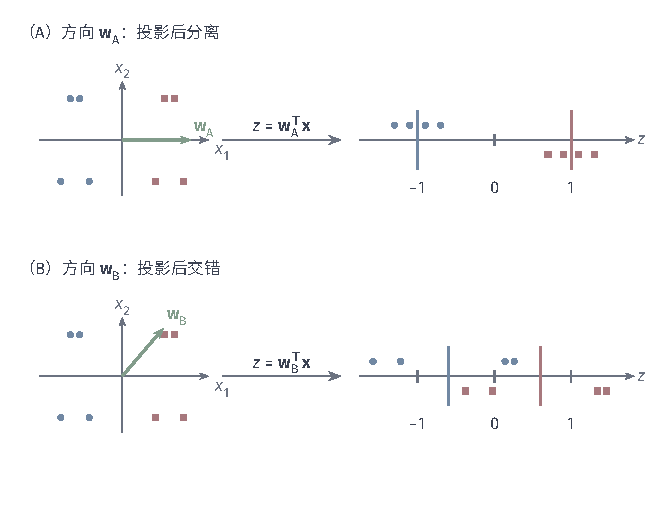
\includegraphics[width=112.000mm]{figures/03-models/01-classic-models/tikz/classification-lda-projection/figure.pdf}
  \caption{同一点集在两个单位方向上的投影。两类各有4点，中心分别为$(-1,0)^{\top}$、$(1,0)^{\top}$，都加上偏移$(-0.3,-1)^{\top}$、$(-0.1,1)^{\top}$、$(0.1,1)^{\top}$、$(0.3,-1)^{\top}$；这是人为构造，坐标无量纲。两行只改变绿色投影方向：$\bm{w}_{\mathrm{A}}=(1,0)^{\top}$与$\bm{w}_{\mathrm{B}}=(3/5,4/5)^{\top}$。右侧按$z=\bm{w}^{\top}\bm{x}$把蓝圆和红方放到同一数轴，彩色短竖线标出各类投影均值；两行共用数轴尺度。}
  \label{fig:classification-lda-projection}
\end{figure}

由于$J$不受$\bm{w}$的非零倍数缩放影响，可以约束$\bm{w}^{\top}\bm{S}_{\mathrm{W}}\bm{w}=1$。对$\bm{w}^{\top}\bm{S}_{\mathrm{B}}\bm{w}-\lambda(\bm{w}^{\top}\bm{S}_{\mathrm{W}}\bm{w}-1)$求导，得到\term{广义特征值问题}（generalized eigenvalue problem）：
\begin{equation}
  \label{eq:classification-fisher-eigenproblem}
  \bm{S}_{\mathrm{B}}\bm{w}
    =\lambda\bm{S}_{\mathrm{W}}\bm{w}.
\end{equation}
驻点还需比较大小。令$\bm{v}=\bm{S}_{\mathrm{W}}^{1/2}\bm{w}$，则
\[
  J(\bm{w})=\frac{\bm{v}^{\top}\bm{A}\bm{v}}{\bm{v}^{\top}\bm{v}},
  \qquad
  \bm{A}=\bm{S}_{\mathrm{W}}^{-1/2}
    \bm{S}_{\mathrm{B}}\bm{S}_{\mathrm{W}}^{-1/2}.
\]
把$\bm{v}$展开到对称半正定矩阵$\bm{A}$的正交特征向量上，上式就是各特征值的加权平均，权重非负且总和为$1$。最大值因而是最大特征值；取对应特征向量，再乘$\bm{S}_{\mathrm{W}}^{-1/2}$，便得到最优Fisher方向。若最大特征值有重数，最优方向未必唯一。

二分类时，令$\bm{h}=\hat{\bm{\mu}}_1-\hat{\bm{\mu}}_2\ne\bm{0}$，由总均值的定义可得
\[
  \bm{S}_{\mathrm{B}}=\frac{n_1n_2}{n}\bm{h}\bm{h}^{\top},
  \qquad
  \bm{w}_{\mathrm{F}}\propto\bm{S}_{\mathrm{W}}^{-1}\bm{h}.
\]
生成式LDA的法向量则为$\bm{w}_{\mathrm{G}}=\hat{\bm{\Sigma}}^{-1}\bm{h}=n\bm{S}_{\mathrm{W}}^{-1}\bm{h}$，两者方向相同。但完整的生成式分类规则还比较
\begin{equation}
  \label{eq:classification-lda-binary-threshold}
  \hat\delta_1(\bm{x})-\hat\delta_2(\bm{x})
    =\bm{w}_{\mathrm{G}}^{\top}
      \left(\bm{x}-\frac{\hat{\bm{\mu}}_1+\hat{\bm{\mu}}_2}{2}\right)
      +\log\frac{\hat\pi_1}{\hat\pi_2}
\end{equation}
的正负。Fisher准则本身只给方向，不给类先验、后验概率或这一阈值。两类均值相同时，均值散度准则没有正特征值方向，而生成模型仍可按先验选择类别。因此Fisher投影可用于非高斯数据，而贝叶斯最优性的证明还需要正确指定的高斯生成模型。

\subsubsection{理论分析}
\label{sec:classification-lda-analysis}

\paragraph{表达能力}
共享协方差高斯模型导出线性判别边界。均值、先验和共同协方差能表达一类目标分布，但类间协方差或多峰性差异可能要求二次边界或更灵活模型。

\paragraph{收敛性}
固定训练集、各类别非空且类内散度正定时，生成式LDA的闭式参数达到该高斯模型的经验似然全局最大值，不需要迭代搜索。累积散度约需$O(nd^2)$运算，分解协方差约需$O(d^3)$运算；奇异情形没有这一正定域内的有限最优解。Fisher投影则通过广义特征值求解达到其比值准则的全局最大值，数值精度与矩阵条件数有关。

\paragraph{泛化性}
计算出经验最优参数后，还要考察样本量增加时估计是否趋近真实参数。\term{一致性}（consistency）正是这种渐近性质；它不表示某个有限训练集上的估计已经准确。

\begin{theorem}[LDA参数估计的一致性]
  \label{thm:classification-lda-consistency}
  设$d$和$C$固定，训练样本独立同分布，真实分布满足式~\eqref{eq:classification-lda-distribution}，且所有$\pi_c^\ast>0$、$\bm{\Sigma}^\ast\succ0$。当$n\to\infty$时，
  \[
    \hat\pi_c\xrightarrow{\mathbb{P}}\pi_c^\ast,\qquad
    \hat{\bm{\mu}}_c\xrightarrow{\mathbb{P}}\bm{\mu}_c^\ast,\qquad
    \hat{\bm{\Sigma}}\xrightarrow{\mathbb{P}}\bm{\Sigma}^\ast .
  \]
  所有类别非空且$\hat{\bm{\Sigma}}$正定的概率趋于$1$。
\end{theorem}

\begin{proof}
  为处理随机的$n_c$，把类均值写成两个全样本平均之比：
  \[
    \hat{\bm{\mu}}_c
      =\frac{n^{-1}\sum_{i=1}^{n}\bm{x}_i\mathbb{1}\{y_i=c\}}
        {n^{-1}\sum_{i=1}^{n}\mathbb{1}\{y_i=c\}} .
  \]
  大数定律使分母收敛到$\pi_c^\ast>0$，分子收敛到$\pi_c^\ast\bm{\mu}_c^\ast$，因而先验和均值都一致。尚未观察到某一类时可以任意约定其均值；该事件的概率趋于零，不影响结论。

  共享协方差估计可展开为
  \[
    \hat{\bm{\Sigma}}
      =\frac1n\sum_{i=1}^{n}\bm{x}_i\bm{x}_i^{\top}
        -\sum_{c=1}^{C}\hat\pi_c
          \hat{\bm{\mu}}_c\hat{\bm{\mu}}_c^{\top}.
  \]
  高斯分布有有限二阶矩，故第一项收敛到
  \[
    \mathbb{E}[\bm{x}\bm{x}^{\top}]
      =\bm{\Sigma}^\ast+
        \sum_{c=1}^{C}\pi_c^\ast
          \bm{\mu}_c^\ast(\bm{\mu}_c^\ast)^{\top}.
  \]
  第二项消去类中心对二阶矩的贡献，余下$\bm{\Sigma}^\ast$。固定维数下，矩阵逐元素收敛也给出算子范数收敛；由$\bm{\Sigma}^\ast$的最小特征值严格为正，估计矩阵以趋于$1$的概率可逆。上述步骤实际上可由强大数定律加强为几乎必然收敛。
\end{proof}

矩阵求逆和$\log\pi_c$在这些条件下连续，所以在参数几乎必然收敛的事件上，对每个固定输入$\bm{x}$，有$\hat\delta_c(\bm{x})\to\delta_c^\ast(\bm{x})$。但$\argmax$在平局处不连续：在真实最大得分唯一的输入处，估计类别最终等于该输入的唯一贝叶斯类别；平局处则未必如此。若最优类别平局的输入集合概率为零，就能进一步推出随机输入上的预测标签收敛。不同贝叶斯分类器在平局处可以选择不同标签，却有相同风险。

参数趋近真实值以后，还需要说明这如何影响独立测试样本上的错误率。分类风险的一致性不必要求标签处处收敛。记$p_c^\ast(\bm{x})$为真实后验，$f^\ast$任选一个贝叶斯规则。由于$\hat f_{\mathrm{LDA}}$最大化$\hat p_c$，逐点有
\begin{equation}
  \label{eq:classification-lda-excess-risk}
  \begin{aligned}
    0&\leq p_{f^\ast(\bm{x})}^\ast(\bm{x})
      -p_{\hat f_{\mathrm{LDA}}(\bm{x})}^\ast(\bm{x})\\
      &\leq 2\max_{1\leq c\leq C}
          |\hat p_c(\bm{x})-p_c^\ast(\bm{x})| .
  \end{aligned}
\end{equation}
这个上界来自在两项之间分别加减相应的估计后验，并利用$\hat p_{\hat f_{\mathrm{LDA}}}\geq\hat p_{f^\ast}$。在参数几乎必然收敛的事件上，后验估计也对每个输入收敛；右端趋于零且不超过$2$。对与训练集独立、来自同一分布的测试输入积分，再用支配收敛定理，得到
\[
  R(\hat f_{\mathrm{LDA}}\mid D_n)
    \longrightarrow R^\ast
    \quad\text{几乎必然},
\]
其中$R(\hat f_{\mathrm{LDA}}\mid D_n)$是给定训练集后的测试错误率，$R^\ast$是贝叶斯错误率。有限样本中无法拟合时可暂用任意固定分类器，这不影响渐近结论。证明依赖正确指定的模型与固定维数，给出风险极限；有限样本速率或维数随样本量增长的情形需要另外分析。Fisher准则评价当前投影的散度比例，承担的是不同的任务。

\subsubsection{支持有监督降维}
\label{sec:classification-lda-reduction}

如果类别多于两个，一条投影轴可能不足以保留类中心之间的差异。把多个广义特征向量作为$\bm{W}\in\mathbb{R}^{d\times r}$的列，就可以把输入转换为$\bm{z}=\bm{W}^{\top}(\bm{x}-\hat{\bm{\mu}})\in\mathbb{R}^{r}$。以下仍假设$\bm{S}_{\mathrm{W}}\succ0$，并取$1\leq r\leq d$。

为避免重复选择同一方向，可要求不同投影轴在类内散度度量下正交：
\begin{equation}
  \label{eq:classification-lda-subspace}
  \max_{\bm{W}}\operatorname{tr}
       (\bm{W}^{\top}\bm{S}_{\mathrm{B}}\bm{W})
  \quad\text{满足}\quad
  \bm{W}^{\top}\bm{S}_{\mathrm{W}}\bm{W}=\bm{I}_r .
\end{equation}
在前述白化坐标中，该问题选择$\bm{A}$最大的$r$个特征值对应的正交方向，因而也就是式~\eqref{eq:classification-fisher-eigenproblem}中最大的$r$个广义特征值方向。

为什么有用的方向至多为$C-1$个？令$\bm{M}\in\mathbb{R}^{d\times C}$的第$c$列为$\sqrt{n_c}(\hat{\bm{\mu}}_c-\hat{\bm{\mu}})$，则
\[
  \bm{S}_{\mathrm{B}}=\bm{M}\bm{M}^{\top},\qquad
  \bm{M}
  \begin{pmatrix}\sqrt{n_1}\\ \vdots\\ \sqrt{n_C}\end{pmatrix}
  =\bm{0}.
\]
右侧列向量非零，说明$\bm{M}$的$C$列线性相关。因此$\operatorname{rank}(\bm{S}_{\mathrm{B}})\leq\min(d,C-1)$；可逆白化不改变秩，$\bm{A}$也至多有这么多个正特征值。若类中心还有额外的线性依赖，实际维数更低。这个限制针对类均值散度，不表示任意分类任务的全部信息都能无损压缩到$C-1$维；例如均值相同而协方差不同的类别，可能被该准则忽略。

LDA投影使用标签，验证时应在每个训练划分内重新估计，并将该投影应用于对应验证样本。得到的低维特征可以交给近邻分类器等后续模型。第\ref{chap:dimensionality-reduction}章按保留信息的目标比较降维方法；其中第\ref{sec:dim-pca}节的PCA保留输入方差而不使用类别标签，LDA则保留类别均值相对于类内波动的判别信息。Fisherfaces人脸识别方法就是借助Fisher准则构造低维判别表示的一个具体例子\scite{belhumeur1997}。

\subsubsection{小结}
\label{sec:classification-lda-summary}

LDA给线性得分提供了两种解释：共享协方差高斯模型给出概率、方向和阈值，Fisher准则则直接选择类中心相对分离的投影。两者在二分类且采用同一类内散度时给出相同方向，但概率解释和风险保证仍依赖额外假设。作为特征变换，LDA也用于语音识别；例如Haeb-Umbach与Ney研究了按语音类别学习线性变换，再与后续识别模型结合的方案\scite{haebumbach1992}。

选用LDA时，需要同时考察分布近似和协方差的可估计性。偏离高斯不必然使分类失效，却使前述最优性证明不再适用；异常样本也会影响均值与协方差。由于$\operatorname{rank}(\bm{S}_{\mathrm{W}})\leq\min(d,n-C)$，当$n-C<d$时估计必然奇异，即使样本稍多于这个界也可能不稳定。降维或收缩协方差可以改善可计算性，但引入了新的选择及偏差，需要用独立验证评估。

\subsection{感知机}
\label{sec:classification-perceptron}

给定线性得分，还可以直接利用预测错误学习权重。\term{感知机}（perceptron）在遇到违反分类条件的样本时修正参数；算法可在任意训练集上运行，正间隔可分性则支持有限更新保证。Rosenblatt在1958年的论文中研究了这一学习机制，本节介绍其中广泛使用的线性阈值模型与误差修正规则\scite{rosenblatt1958}。

康奈尔航空实验室还用Mark I Perceptron将这一研究路线实现为电子装置。历史系统包含感觉、关联和响应等组织；本节抽取的是后来常用的单个线性分类器及其更新规则\scite{smithsonianMarkI}。

\subsubsection{模型结构}
\label{sec:classification-perceptron-model}

本小节先使用二分类标签$y_i\in\{-1,+1\}$。为了使偏置在更新规则和收敛证明中始终处于同一坐标系，引入\term{增广向量}（augmented vector），即在输入末尾补一个恒为$1$的分量，并把偏置并入参数：
\begin{equation}
  \label{eq:classification-perceptron-augmented}
  \tilde{\bm{x}}=
    \begin{pmatrix}\bm{x}\\1\end{pmatrix},\qquad
  \tilde{\bm{w}}=
    \begin{pmatrix}\bm{w}\\b\end{pmatrix}
    \in\mathbb{R}^{d+1}.
\end{equation}
其中$\bm{w}\in\mathbb{R}^{d}$，$b\in\mathbb{R}$。分类规则为
\begin{equation}
  \label{eq:classification-perceptron-prediction}
  f(\bm{x})=\operatorname{sign}
    (\tilde{\bm{w}}^{\top}\tilde{\bm{x}})
    =\operatorname{sign}(\bm{w}^{\top}\bm{x}+b).
\end{equation}
约定$\operatorname{sign}(s)=+1$当$s\geq0$，否则为$-1$。非退化边界$\bm{w}^{\top}\bm{x}+b=0$是在$d$维输入空间中的$(d-1)$维超平面。它与二分类LDA具有相同的边界形式；这里的参数来自错误反馈，输出是类别得分与标签，概率需要另建模型。

在这一表示下，正间隔可分是指存在单位向量$\bm{u}^\ast\in\mathbb{R}^{d+1}$和$\gamma>0$，使
\begin{equation}
  \label{eq:classification-perceptron-margin}
  \begin{aligned}
    y_i\langle\bm{u}^\ast,\tilde{\bm{x}}_i\rangle
      &\geq\gamma,\qquad i=1,\ldots,n,\\
    \|\bm{u}^\ast\|_2&=1,\qquad
    \|\tilde{\bm{x}}_i\|_2\leq R .
  \end{aligned}
\end{equation}
这里$R$约束的是增广输入，因此$R\geq\max_i\sqrt{\|\bm{x}_i\|_2^2+1}$。$\gamma$也是增广空间中的间隔；若$\bm{u}^\ast=(\bm{v}^{\top},a)^{\top}/\sqrt{\|\bm{v}\|_2^2+a^2}$，其分母包含偏置$a$，不同于原输入空间中以$\|\bm{v}\|_2$归一化的几何距离。有限训练集只要能被仿射超平面严格分开，就存在这样的正$\gamma$。

线性表示的边界也很具体。例如异或任务把$(0,0)$、$(1,1)$标为负类，把$(1,0)$、$(0,1)$标为正类。按上述平局规则，前两点要求$b<0$和$w_1+w_2+b<0$，后两点要求$w_1+b\geq0$和$w_2+b\geq0$。前两式相加与后两式相加，对同一个$w_1+w_2+2b$给出矛盾要求。Minsky与Papert在1969年的《Perceptrons》中系统研究了此类表示能力限制；改变输入特征或加入非线性隐藏层可以越过单个线性边界的限制，但那已经改变了模型族\scite{minsky1969}。

\subsubsection{参数学习}
\label{sec:classification-perceptron-learning}

从$\tilde{\bm{w}}^{(0)}=\bm{0}$出发，若当前样本满足$y_i\langle\tilde{\bm{w}}^{(t)},\tilde{\bm{x}}_i\rangle\leq0$，便进行一次更新：
\begin{equation}
  \label{eq:classification-perceptron-update}
  \tilde{\bm{w}}^{(t+1)}
    =\tilde{\bm{w}}^{(t)}+\eta y_i\tilde{\bm{x}}_i,
    \qquad \eta>0 .
\end{equation}
这里$t$只数实际更新，学习率$\eta$保持不变。拆开最后一个分量，就是$\bm{w}\leftarrow\bm{w}+\eta y_i\bm{x}_i$和$b\leftarrow b+\eta y_i$。同一个样本的有符号得分增加$\eta\|\tilde{\bm{x}}_i\|_2^2$，所以更新确实朝修正当前判断的方向移动；但它可能同时破坏其他样本的正确分类，因而需要反复遍历。零得分也触发更新，即使按平局规则恰好预测为正确的正类，仍要求它离开边界。

\begin{algorithm}[带遍历上限的感知机训练]
  \label{alg:classification-perceptron}
  \begin{algorithmic}[1]
    \Require $D_n$，固定学习率$\eta>0$，最大遍历轮数$E\geq1$
    \Ensure 参数$\tilde{\bm{w}}$与是否已验证收敛的状态
    \State $\tilde{\bm{w}}\gets\bm{0}$
    \For{$e=1,\ldots,E$}
      \State $m\gets0$
      \For{$i=1,\ldots,n$}
        \State $\tilde{\bm{x}}_i\gets(\bm{x}_i^{\top},1)^{\top}$
        \If{$y_i\langle\tilde{\bm{w}},\tilde{\bm{x}}_i\rangle\leq0$}
          \State $\tilde{\bm{w}}\gets\tilde{\bm{w}}+\eta y_i\tilde{\bm{x}}_i$
          \State $m\gets m+1$
        \EndIf
      \EndFor
      \If{$m=0$}
        \State \Return $(\tilde{\bm{w}},\text{已收敛})$
      \EndIf
    \EndFor
    \State \Return $(\tilde{\bm{w}},\text{达到轮数上限})$
  \end{algorithmic}
\end{algorithm}

一整轮没有更新时，所有样本都是在同一个参数下得到严格正的有符号得分，才构成收敛证据。达到轮数上限时返回的是预算内的当前解，可分性仍未由这一停止状态判定。稠密实现每轮需要$O(nd)$运算，除训练集外只需$O(d)$参数空间；样本访问顺序可以改变输出的分隔面。

从优化角度看，定义\term{感知机损失}（perceptron loss）
\begin{equation}
  \label{eq:classification-perceptron-loss}
  \ell_{\mathrm{P}}(\tilde{\bm{w}};\bm{x}_i,y_i)
    =\max\{0,-y_i\langle\tilde{\bm{w}},\tilde{\bm{x}}_i\rangle\}.
\end{equation}
负得分处的梯度为$-y_i\tilde{\bm{x}}_i$，正得分处为$\bm{0}$；零得分处选择次梯度$-y_i\tilde{\bm{x}}_i$，就得到式~\eqref{eq:classification-perceptron-update}。这是逐样本次梯度更新；随机抽取样本时才相应成为随机次梯度下降。这里使用的是零间隔损失，不是标准的\term{合页损失}（hinge loss）$\max\{0,1-y_i\langle\tilde{\bm{w}},\tilde{\bm{x}}_i\rangle\}$。前者在零参数处就对所有样本取零，因此“感知机损失为零”本身不能证明分类正确；算法在零得分处仍更新的约定不可省略。

\subsubsection{理论分析}
\label{sec:classification-perceptron-analysis}

\paragraph{表达能力}
单层感知机只表示一个线性分界，异或等非线性模式不在原始候选空间内。添加特征映射改变分界族，改变更新轮数本身则不改变表示能力。

\paragraph{收敛性}
每次修正可能破坏已有判断，为什么这些修正不会无穷持续？关键是存在一个始终把所有样本分对的参考方向：更新朝该方向取得线性累积的进展，而参数范数的平方只能线性增长。Novikoff在1962年报告的证明清楚展示了这两个增长速度之间的矛盾\scite{novikoff1962}。

\begin{theorem}[感知机的错误更新界]
  \label{thm:classification-perceptron-mistakes}
  若$D_n$满足式~\eqref{eq:classification-perceptron-margin}，从零参数出发，以固定$\eta>0$按式~\eqref{eq:classification-perceptron-update}更新，则对任意样本访问顺序，错误更新次数$M$满足
  \[
    M\leq\left(\frac R\gamma\right)^2 .
  \]
  这里错误更新包括零得分时的更新。若持续完整遍历训练集，且不因预算提前退出，算法在有限轮后得到所有训练样本上有符号得分均严格为正的参数。
\end{theorem}

\begin{proof}
  设第$t+1$次更新使用样本$i_t$。沿单位参考方向$\bm{u}^\ast$考察更新，得到
  \begin{align*}
    \langle\tilde{\bm{w}}^{(t+1)},\bm{u}^\ast\rangle
      &=\langle\tilde{\bm{w}}^{(t)},\bm{u}^\ast\rangle
        +\eta y_{i_t}\langle\tilde{\bm{x}}_{i_t},\bm{u}^\ast\rangle\\
      &\geq\langle\tilde{\bm{w}}^{(t)},\bm{u}^\ast\rangle+\eta\gamma .
  \end{align*}
  从零参数累加$M$次，便有
  \[
    \langle\tilde{\bm{w}}^{(M)},\bm{u}^\ast\rangle
      \geq M\eta\gamma .
  \]
  另一方面，展开更新后的平方范数：
  \begin{align*}
    \|\tilde{\bm{w}}^{(t+1)}\|_2^2
      &=\|\tilde{\bm{w}}^{(t)}\|_2^2
        +2\eta y_{i_t}
          \langle\tilde{\bm{w}}^{(t)},\tilde{\bm{x}}_{i_t}\rangle\\
      &\quad+\eta^2\|\tilde{\bm{x}}_{i_t}\|_2^2\\
      &\leq\|\tilde{\bm{w}}^{(t)}\|_2^2+\eta^2R^2 .
  \end{align*}
  不等式使用了更新条件：交叉项非正；并使用同一增广空间中的长度界$R$。再次累加，得到$\|\tilde{\bm{w}}^{(M)}\|_2^2\leq M\eta^2R^2$。由Cauchy--Schwarz不等式和$\|\bm{u}^\ast\|_2=1$，
  \[
    M\eta\gamma
      \leq\langle\tilde{\bm{w}}^{(M)},\bm{u}^\ast\rangle
      \leq\|\tilde{\bm{w}}^{(M)}\|_2
      \leq\eta R\sqrt{M}.
  \]
  $M=0$时结论直接成立；$M>0$时除以$\eta\sqrt M$再平方，得到所述界。因此更新不可能无限发生。持续完整遍历会在最后一次更新之后再检查所有样本；若仍有非正得分就还会更新，产生矛盾，故最终必有一整轮没有更新。
\end{proof}

这个界不显式含$n$，也不依赖访问顺序，但$R$和$\gamma$随数据而定；增加样本可能缩小可分间隔。它只约束更新次数，不包括寻找错误时检查正确样本的开销。对于算法~\ref{alg:classification-perceptron}的逐轮扫描，若不提前截断，至多需要$M+1$轮，包括最终的无更新确认轮。

若数据不可分，有限更新保证失效，持续遍历可能反复更新，此时可以限制训练预算并保留历史较好解，或采用允许间隔违约的在线方法。这些处理改变了停止或选解方式，仍须分别分析。

\paragraph{泛化性}
测试风险需要训练更新之外的统计条件。前述错误次数证明只考察给定样本的几何结构；若要判断未来预测，需要规定抽样分布与训练后返回哪个分类器。Cesa-Bianchi、Conconi与Gentile在2004年研究了这种联系：由独立同分布样本上的在线表现控制历史预测规则的风险，并讨论相应的输出选择方法\scite{cesabianchi2004generalization}。

下面给出一个期望风险的简单结论，说明额外条件怎样进入证明。按独立同分布的到达顺序，仅遍历$D_n$一次，从零参数出发使用固定学习率$\eta>0$和原更新规则。用$f_i$表示看到第$i$个样本之前的分类器；它只依赖$D_{i-1}$，其中$D_0$为空。这里$i$计数已访问的样本位置，与只计实际更新的$t$不同。训练后独立地从$\{1,\ldots,n\}$均匀抽取$I$，返回$f_I$，使输出规则与下述期望风险证明一致。

\begin{theorem}[随机历史分类器的期望风险]
  \label{thm:classification-perceptron-risk}
  设训练样本独立同分布，测试样本独立来自同一分布。假设存在固定的单位向量$\bm{u}^\ast$及常数$R<\infty$、$\gamma>0$，使
  \[
    \|\tilde{\bm{x}}\|_2\leq R,\qquad
    y\langle\bm{u}^\ast,\tilde{\bm{x}}\rangle\geq\gamma
    \quad\text{几乎必然}.
  \]
  对上述单遍历训练和随机输出规则，有
  \begin{equation}
    \label{eq:classification-perceptron-risk}
    \mathbb{E}_{D_n,I}\!\left[R(f_I\mid D_n,I)\right]
      \leq\frac{R^2}{n\gamma^2}.
  \end{equation}
\end{theorem}

\begin{proof}
  令$e_i=\mathbb{1}\{f_i(\bm{x}_i)\ne y_i\}$。由于$f_i$尚未使用第$i$个样本，独立性给出
  \[
    \mathbb{E}[e_i\mid D_{i-1}]
      =R(f_i\mid D_{i-1}).
  \]
  对两边取期望，再对均匀的$I$平均，就有
  \[
    \mathbb{E}_{D_n,I}[R(f_I\mid D_n,I)]
      =\frac1n\sum_{i=1}^{n}\mathbb{E}[e_i].
  \]
  每次预测错误都会触发更新，零得分且预测正确时也可能更新，故$\sum_i e_i\leq M$。分布层面的共同间隔和长度界使定理~\ref{thm:classification-perceptron-mistakes}几乎必然适用于每个训练序列，于是$M\leq R^2/\gamma^2$，代入即得结论。
\end{proof}

这里的$R$和$\gamma$约束整个数据分布。式~\eqref{eq:classification-perceptron-risk}对训练抽样及随机历史状态取平均；当上界小于$1$时，它提供非平凡的期望风险控制。最终参数、平均参数或多轮训练使用不同的输出与依赖关系，需各自分析：尤其在多轮中，当前样本已经参与既有参数的形成。投票感知机等扩展正是在利用训练历史的方式上作出新的选择。

\subsubsection{支持多分类}
\label{sec:classification-perceptron-multiclass}

对$C$类问题，把标签改为$y_i\in\{1,\ldots,C\}$，每类维护一组增广参数$\tilde{\bm{w}}_c=(\bm{w}_c^{\top},b_c)^{\top}$，得分和预测为
\[
  s_c(\bm{x})=\langle\tilde{\bm{w}}_c,\tilde{\bm{x}}\rangle,
  \qquad
  \hat y=\argmax_{c\in\{1,\ldots,C\}}s_c(\bm{x}).
\]
平局仍按最小类别索引处理。这个构造把正确类别的得分与每个竞争类别作比较，也可用\term{Kesler构造}（Kesler construction）把这些比较写成一个扩展空间中的线性可分问题。

遇到$\hat y_i\ne y_i$时，只提高正确类别的参数并降低错误获胜类别的参数：
\begin{equation}
  \label{eq:classification-perceptron-multiclass-update}
  \begin{aligned}
    \tilde{\bm{w}}_{y_i}
      &\leftarrow\tilde{\bm{w}}_{y_i}+\eta\tilde{\bm{x}}_i,\\
    \tilde{\bm{w}}_{\hat y_i}
      &\leftarrow\tilde{\bm{w}}_{\hat y_i}-\eta\tilde{\bm{x}}_i .
  \end{aligned}
\end{equation}
其余类别不变，两个类别的偏置也随各自最后一个分量同时更新。若平局后预测错误，同样更新；若已选择正确类别，则该规则不更新。与二分类中所有零得分均更新的约定不同，这里直接按最终预测是否正确判断。

收敛条件也必须改为多类的得分差条件。把各类参数按行堆成$\tilde{\bm{W}}\in\mathbb{R}^{C\times(d+1)}$；假设存在$\|\bm{U}^\ast\|_{\mathrm{F}}=1$和$\gamma_{\mathrm{mc}}>0$，使对所有$i$和$c\ne y_i$都有
\[
  \langle\bm{U}_{y_i,:}^\ast-\bm{U}_{c,:}^\ast,
    \tilde{\bm{x}}_i\rangle\geq\gamma_{\mathrm{mc}} .
\]
这里$\|\cdot\|_{\mathrm{F}}$是所有矩阵元素平方和的平方根，行向量的内积按对应坐标计算。一次更新的方向矩阵仅两行非零，分别为$\tilde{\bm{x}}_i^{\top}$与$-\tilde{\bm{x}}_i^{\top}$，其平方范数至多为$2R^2$。它与$\bm{U}^\ast$的内积至少为$\gamma_{\mathrm{mc}}$；与当前参数的内积则为$s_{y_i}(\bm{x}_i)-s_{\hat y_i}(\bm{x}_i)\leq0$。因此零初始化时完全沿用二分类证明，得到
\[
  M\eta\gamma_{\mathrm{mc}}
    \leq\|\tilde{\bm{W}}^{(M)}\|_{\mathrm{F}}
    \leq\eta R\sqrt{2M},
  \qquad
  M\leq\frac{2R^2}{\gamma_{\mathrm{mc}}^2}.
\]
有限更新保证因而保留下来，但它要求所有正确类与竞争类之间都具有共同的正间隔，而不是只检查任意一对类别。

\subsubsection{小结}
\label{sec:classification-perceptron-summary}

感知机通过逐样本错误反馈学习线性边界；正间隔可分时，有限次更新能够找到可行分隔面。可行面之间怎样选择、不可分数据怎样返回，以及非线性关系怎样表示，分别引出下面的扩展。

\term{口袋算法}（Pocket algorithm）处理的是“当前权重未必比过去更好”的问题。常用的带历史最优记录的版本额外保存$\tilde{\bm{w}}_{\mathrm{pocket}}$：每次检查候选参数时，计算全训练集零一错误数，仅在严格改进时替换记录；预算用尽后返回记录参数。它适用于噪声或矛盾标签数据，返回预算内已检查候选中的最小训练错误解；每次候选比较还需要评估全训练集。Gallant在1990年的论文中系统讨论了Pocket及相关学习方法\scite{gallant1990}。

若问题在于原空间不能线性分开，可把输入换成特征映射$\bm{\phi}(\bm{x})$。核函数$K(\bm{x},\bm{z})=\langle\bm{\phi}(\bm{x}),\bm{\phi}(\bm{z})\rangle$直接计算映射后的内积，省去显式构造高维坐标，得到\term{核感知机}（kernel perceptron）。为与前文偏置一致，使用增广映射$(\bm{\phi}(\bm{x}),1)$及其核$\tilde K(\bm{x},\bm{z})=K(\bm{x},\bm{z})+1$。零初始化、单位学习率下，参数在特征空间中是更新样本的线性组合，预测可写为
\begin{equation}
  \label{eq:classification-kernel-perceptron}
  f(\bm{x})=\operatorname{sign}
    \left(\sum_{i=1}^{n}\alpha_i y_i
      [K(\bm{x}_i,\bm{x})+1]\right).
\end{equation}
这里$\alpha_i$是样本$i$的更新次数；遇到非正有符号得分时令$\alpha_i\leftarrow\alpha_i+1$。必须选用正定核，即它在任意有限输入集上生成半正定Gram矩阵，才能作上述内积解释；有限更新还要求增广特征空间内存在正间隔，长度界相应变为$\sqrt{K(\bm{x}_i,\bm{x}_i)+1}$的上界。预测需要访问系数非零的样本，数量可能随训练增长。将内积推广到特征空间的思路可追溯至Aizerman、Braverman与Rozonoer在1964年的势函数研究\scite{aizerman1964}。

另一类扩展保留多段训练历史。\term{投票感知机}（voted perceptron）保存历次参数$\tilde{\bm{w}}^{(j)}$及其使用时长$q_j$，以时长作为票数：
\[
  f_{\mathrm{vote}}(\bm{x})
    =\operatorname{sign}\left(
      \sum_{j=1}^{J}q_j
        \operatorname{sign}
          (\langle\tilde{\bm{w}}^{(j)},\tilde{\bm{x}}\rangle)
      \right).
\]
其中$J$为保存的参数状态数，$q_j$按该参数持续使用的样本步数计数，而不只数更新次数。\term{平均感知机}（averaged perceptron）则对相同历史平均参数，
\[
  \bar{\tilde{\bm{w}}}
    =\frac{\sum_{j=1}^{J}q_j\tilde{\bm{w}}^{(j)}}
      {\sum_{j=1}^{J}q_j},
  \qquad
  f_{\mathrm{avg}}(\bm{x})
    =\operatorname{sign}
       (\langle\bar{\tilde{\bm{w}}},\tilde{\bm{x}}\rangle).
\]
平均向量可通过累计和维护，预测仍只需一次线性得分；投票则需保留多个状态。先取符号再投票与先平均再取符号一般不等价。Freund与Schapire在1999年的工作中研究了投票法，也比较了平均法；其大间隔泛化结论依赖论文中规定的抽样、训练与输出设置\scite{freund1999}。

若希望每次更新不仅改正符号，还达到指定得分间隔，\term{被动攻击算法}（passive-aggressive algorithm, PA）把“尽量少改参数”和“满足当前样本的单位间隔”合成一个投影问题。用$\bm{v}$表示待求的新增广参数，
\begin{equation}
  \label{eq:classification-pa-projection}
  \begin{aligned}
    \min_{\bm{v}}\quad&
      \frac12\|\bm{v}-\tilde{\bm{w}}\|_2^2\\
    \text{满足}\quad&
      y_i\langle\bm{v},\tilde{\bm{x}}_i\rangle\geq1 .
  \end{aligned}
\end{equation}
令$\ell_i=\max\{0,1-y_i\langle\tilde{\bm{w}},\tilde{\bm{x}}_i\rangle\}$。约束已满足时参数不变；否则，拉格朗日驻点要求$\bm{v}=\tilde{\bm{w}}+\tau_i y_i\tilde{\bm{x}}_i$，将活跃约束代回即得
\[
  \tau_i=\frac{\ell_i}{\|\tilde{\bm{x}}_i\|_2^2},
  \qquad
  \tilde{\bm{w}}\leftarrow
    \tilde{\bm{w}}+\tau_i y_i\tilde{\bm{x}}_i .
\]
因此PA在间隔足够时“被动”，不足时按违约大小调整。增广方式也意味着这里把偏置变化纳入距离惩罚。噪声下硬性满足当前样本可能调整过大，PA-I可用$\tau_i=\min\{\lambda_{\mathrm{PA}},\ell_i/\|\tilde{\bm{x}}_i\|_2^2\}$限制步长，其中$\lambda_{\mathrm{PA}}>0$控制容忍程度。Crammer等人的2006年论文统一分析了这些在线大间隔方法；其保证针对在线更新的损失与间隔行为\scite{crammer2006}。

如果输出是一整条词性序列等组合对象，可以把多分类的得分比较推广到结构之间。\term{结构化感知机}（structured perceptron）用联合特征$\bm{\phi}(\bm{x},y)$描述输入与候选结构，预测
\[
  \hat y_i=\argmax_{y\in Y(\bm{x}_i)}
    \langle\bm{\theta},\bm{\phi}(\bm{x}_i,y)\rangle ,
\]
其中$Y(\bm{x}_i)$是候选结构集合，$\bm{\theta}$是与联合特征同维的参数。解码错误时进行
\[
  \bm{\theta}\leftarrow\bm{\theta}
    +\eta\bigl[\bm{\phi}(\bm{x}_i,y_i)
      -\bm{\phi}(\bm{x}_i,\hat y_i)\bigr].
\]
需要的类别或结构偏置也作为联合特征中的相应指示分量处理；对所有候选都相同的常数项会在得分差中消去。在特征差有界、正确结构与所有错误结构之间正间隔可分、且能精确解码的条件下，可沿用多类证明。近似解码的误差改变了更新条件，需纳入相应分析。Collins在2002年将这种更新与参数平均用于序列标注，提供了词性标注和短语识别等实例，也为比较感知机与条件随机场等结构化模型提供了参照\scite{collins2002}。

Pocket选择返回的历史解，核方法改变输入表示，投票与平均组合训练轨迹，PA规定单步调整目标，结构化感知机扩展输出与解码。方法选择可据此定位问题所在，再检查相应的可分性条件、计算预算与风险保证。
\subsection{支持向量机（SVM）}
\label{sec:classification-svm}

感知机回答了一个基本问题：如果训练样本能够被某个超平面分开，怎样通过错误驱动的更新找到一个分离器？但分开训练样本并不意味着分界的位置已经合适。同一批可分数据往往允许许多分离超平面，即使从零参数开始，感知机的结果仍会受样本顺序和更新规则影响。一个紧贴训练样本的边界虽然没有训练错误，却可能在输入受到很小扰动时改变预测。要在这些分离器之间作出选择，还需要说明什么样的边界更值得保留。

\term{支持向量机}（support vector machine，SVM）以训练样本到边界的距离选择分隔面：在正确分离样本的前提下，增大最近样本到边界的距离，称为最大间隔。给定特征表示与距离度量后，这个几何准则使边界具有可比较的尺度。不可分数据可以通过松弛约束处理，非线性关系则可以通过改变特征表示处理；两种扩展分别作用于误差容忍与候选函数。

最优分离超平面的早期研究可以追溯到20世纪60年代。现代支持向量分类器的一项关键进展，是Boser、Guyon与Vapnik在1992年把最优间隔训练和核表示结合起来\scite{boser1992margin}。这篇论文从分类器容量与泛化之间的关系出发，用最靠近边界的支持样本表示解，并研究了多项式和径向基等非线性分类函数。在高阶多项式情形中，显式列出全部交互特征可能难以承受，而只计算样本间的核函数可以避开这一展开。论文中的字符识别实验也让这种表示方式与具体分类任务联系起来。

1995年Cortes与Vapnik进一步系统发展了容许训练样本违反间隔约束的支持向量网络\scite{cortes1995}。这样，无法严格分开的数据也能进入带有惩罚的优化问题，间隔不再以训练样本全部正确为前提。沿着这条路线，模型表达、误差容忍与实际求解逐渐形成分工：核函数决定怎样比较输入，松弛惩罚决定怎样对待间隔违反，后面介绍的分解算法则降低每次优化所需处理的问题规模。几何建模、凸优化和统计分析因此相互联系，但仍分别回答选择什么模型、如何求解以及怎样控制新样本误差。

硬间隔以精确分类约束建立基准问题，软间隔加入训练损失，核表示扩展候选得分，多分类组织类别竞争。下面用拉格朗日乘子和KKT条件推导对偶、恢复支持向量并解释SMO更新（工具参考\BookSectionRef{sec:opt-multiplier-dual-methods}{第一卷“数学准备”的“基于乘子与对偶的求解”小节}）；核合法性的依据见第\ref{sec:classic-overview-kernel-validity}节。新样本风险另按函数类复杂度与正则化学习的稳定性分析（稳定性框架参考\BookChapterRef{chap:convex-learning-and-stability}{第二卷“基础、理论和可信性”的“一般学习的可学习性”章}）。

\subsubsection{模型结构}
\label{sec:classification-svm-model}

沿用二分类标签约定，设训练集为$D_n=\{(\bm{x}_i,y_i)\}_{i=1}^n$，其中$\bm{x}_i\in\mathbb{R}^d$、$y_i\in\{-1,+1\}$，并假设两类均非空。令实值得分为$g(\bm{x})=\bm{w}^{\top}\bm{x}+b$，其中$\bm{w}\in\mathbb{R}^d$、$b\in\mathbb{R}$且$\bm{w}\ne\bm{0}$。决策超平面是$g(\bm{x})=0$，预测规则为$\hat y(\bm{x})=\operatorname{sign}(g(\bm{x}))$；若得分恰为零，约定预测为$+1$。后文会将零得分保守地计入间隔错误，因此这个平局约定不影响风险上界。

仅比较$y_i g(\bm{x}_i)$还不能比较不同超平面。把$(\bm{w},b)$同时乘以任意正数，分类结果不变，这个数值却会随之放大。为区分参数尺度与真实距离，定义样本的\term{函数间隔}（functional margin）为$m_i=y_i g(\bm{x}_i)$，定义其\term{几何间隔}（geometric margin）为
\begin{equation}
  \gamma_i
  =\frac{y_i(\bm{w}^{\top}\bm{x}_i+b)}
         {\lVert\bm{w}\rVert_2},
  \qquad
  \gamma=\min_{1\le i\le n}\gamma_i.
  \label{eq:classification-svm-margin}
\end{equation}
函数间隔保留了得分的尺度；几何间隔除以法向量长度，得到沿法向方向测量的有符号距离。样本分类正确时，这个距离为正。若输入改变为$\bm{x}_i+\bm{\Delta}$，由Cauchy--Schwarz不等式可得
\[
  y_i g(\bm{x}_i+\bm{\Delta})
  \ge y_i g(\bm{x}_i)
      -\lVert\bm{w}\rVert_2\lVert\bm{\Delta}\rVert_2.
\]
因此，$\lVert\bm{\Delta}\rVert_2<\gamma_i$时预测不会翻转。这说明间隔量化当前特征空间中、由该范数限定的输入扰动容忍程度；分布变化需要另外规定变化方式。

严格线性可分意味着存在$(\bm{w},b)$使所有$m_i>0$。由于样本数有限，可以将这组参数除以$\min_i m_i$，得到$\min_i m_i=1$的规范化表示。在该表示下，最近样本到决策超平面的单侧距离为$1/\lVert\bm{w}\rVert_2$；两个平行超平面$g(\bm{x})=+1$与$g(\bm{x})=-1$之间的总宽度则是$2/\lVert\bm{w}\rVert_2$。本节将前者记为$\gamma$，不把单侧间隔与两侧带宽混用。

最大化$\gamma$于是等价于最小化$\lVert\bm{w}\rVert_2$。平方与正比例因子不改变最优解，却使求导更方便，得到\term{硬间隔}（hard margin）SVM的原始问题：
\begin{equation}
  \begin{aligned}
    \min_{\bm{w},b}\quad&
      \frac12\lVert\bm{w}\rVert_2^2\\
    \text{s.t.}\quad&
      y_i(\bm{w}^{\top}\bm{x}_i+b)\ge1,
      \quad i=1,\ldots,n.
  \end{aligned}
  \label{eq:classification-svm-hard-primal}
\end{equation}
这里的“硬”表示每个样本都必须满足间隔约束，不能用其他样本的改善来补偿某个样本的违反。约束写为大于等于$1$并没有放弃规范化：若一个可行解的最小函数间隔严格大于$1$，将参数一起缩小就能降低目标，所以最优解必有紧约束。

\begin{theorem}[硬间隔解的存在性与唯一性]
  \label{thm:classification-svm-hard-unique}
  若有限训练集严格线性可分且两类均非空，则问题\eqref{eq:classification-svm-hard-primal}存在唯一的规范化最优参数$(\bm{w}^{\ast},b^{\ast})$。目标函数只对$\bm{w}$严格凸，偏置的唯一性还需要两类约束共同确定。
\end{theorem}
\begin{proof}
取一个可行解，并把目标限制在不超过该解目标值的水平集上，则$\bm{w}$有界。固定一个正类样本与一个负类样本，它们的约束分别给出$b$的下界与上界；因为$\bm{w}$有界，$b$也有界。该水平集闭且非空，因此连续目标能在其中取得最小值。

若两个最优解的权重不同，其平均仍可行，但平方范数的严格凸性会使平均解的目标更小，产生矛盾。因此所有最优解共享同一个$\bm{w}^{\ast}$。为研究$b$，对给定$\bm{w}$定义两类样本的投影端点
\[
  a_+(\bm{w})=\min_{i:y_i=+1}\bm{w}^{\top}\bm{x}_i,
  \qquad
  a_-(\bm{w})=\max_{i:y_i=-1}\bm{w}^{\top}\bm{x}_i.
\]
可行偏置恰好满足
\[
  1-a_+(\bm{w})\le b\le-1-a_-(\bm{w}),
\]
所以投影间距$a_+(\bm{w})-a_-(\bm{w})$至少为$2$。若在最优$\bm{w}^{\ast}$处它严格大于$2$，令$\theta=2/(a_+-a_-)<1$，取新权重$\theta\bm{w}^{\ast}$和新偏置$-\theta(a_++a_-)/2$，则两类最近样本的函数间隔都为$1$，其余样本仍满足约束，而非零权重的范数严格减小。这与最优性矛盾。故最优投影间距只能等于$2$，可行偏置区间收缩为单点，$b^{\ast}$也唯一。
\end{proof}

这个证明还表明，最优解的两个支持超平面都至少接触一个训练样本。唯一性属于固定数据与固定特征表示下的规范化硬间隔问题，不意味着更换特征、加入噪声或放松约束以后仍有同样的结论。

\begin{example}[单侧间隔与带宽]
  \label{ex:classification-svm-one-dimensional}
  考虑一维教学数据$(x_1,y_1)=(-1,-1)$、$(x_2,y_2)=(1,+1)$、$(x_3,y_3)=(-2,-1)$和$(x_4,y_4)=(2,+1)$。任意落在$-1$与$1$之间的阈值都能正确分类，但只有阈值$0$使两侧最近距离的较小者达到最大。规范化最优解为$w^{\ast}=1$、$b^{\ast}=0$；最近样本的单侧距离为$1$，两条支持超平面在此退化为两个点$-1$与$1$，其间距离为$2$。更远的两个样本不限制这一最优间隔。
\end{example}

\subsubsection{参数学习}
\label{sec:classification-svm-learning}

每个间隔约束对最优边界的影响，可由对应的拉格朗日乘子表示。\term{对偶问题}（dual problem）把这些约束权重作为优化变量，既揭示参与预测的样本，也把训练表示为样本间内积运算，为核化提供入口。原始与对偶的变量数分别受特征维数和样本数影响，计算选择还要结合求解器与数据稀疏性。

将约束写为$1-y_i(\bm{w}^{\top}\bm{x}_i+b)\le0$，引入$\alpha_i\ge0$，记$\bm{\alpha}=(\alpha_1,\ldots,\alpha_n)^{\top}$。拉格朗日函数为
\begin{equation}
  \begin{aligned}
    L(\bm{w},b,\bm{\alpha})
    ={}&\frac12\lVert\bm{w}\rVert_2^2\\
      &+\sum_{i=1}^n\alpha_i
        \bigl[1-y_i(\bm{w}^{\top}\bm{x}_i+b)\bigr].
  \end{aligned}
  \label{eq:classification-svm-hard-lagrangian}
\end{equation}
对一个可行$(\bm{w},b)$，$\sup_{\bm{\alpha}\ge\bm{0}}L$等于原始目标；若有约束违反，对应乘子趋于无穷会使上确界为正无穷。因此原始最优值可写为$\inf_{\bm{w},b}\sup_{\bm{\alpha}\ge\bm{0}}L$。反过来，先对$(\bm{w},b)$取下确界再最大化，得到原始最优值的下界。强对偶条件决定两种次序何时给出相同值。

这里可以直接核验\term{Slater条件}（Slater's condition）：它要求存在严格满足不等式约束的点。取一个严格分离器，并把参数放大到所有函数间隔都严格大于$1$，就得到所需点。结合目标凸、约束仿射以及上一小节的最优值可达性，可得强对偶与最优乘子的存在性。

现在计算$q(\bm{\alpha})=\inf_{\bm{w},b}L(\bm{w},b,\bm{\alpha})$。由于$b$没有二次项，若$\sum_i\alpha_i y_i\ne0$，沿$b$的某个方向就有$L\to-\infty$。要使$q$有限，必须满足等式约束；关于$\bm{w}$的极小值则由驻点给出：
\begin{equation}
  \bm{w}=\sum_{i=1}^n\alpha_i y_i\bm{x}_i,
  \qquad
  \sum_{i=1}^n\alpha_i y_i=0.
  \label{eq:classification-svm-stationarity}
\end{equation}
令$\bm{v}=\sum_i\alpha_i y_i\bm{x}_i$，代入后涉及权重的两项变为$\frac12\lVert\bm{v}\rVert_2^2-\lVert\bm{v}\rVert_2^2$，而$b$项为零。展开$\lVert\bm{v}\rVert_2^2$，便得到
\begin{equation}
  \begin{aligned}
    \max_{\bm{\alpha}}\quad&
      q(\bm{\alpha})
      =\sum_{i=1}^n\alpha_i
       -\frac12\sum_{i,j=1}^n
          \alpha_i\alpha_j y_i y_j
          \bm{x}_i^{\top}\bm{x}_j\\
    \text{s.t.}\quad&
      \sum_{i=1}^n\alpha_i y_i=0,\qquad
      \alpha_i\ge0,\quad i=1,\ldots,n.
  \end{aligned}
  \label{eq:classification-svm-hard-dual}
\end{equation}
二次项矩阵的元素为$\bm{Q}_{i,j}=y_i y_j\bm{x}_i^{\top}\bm{x}_j$。对任意$\bm{a}\in\mathbb{R}^n$，有$\bm{a}^{\top}\bm{Q}\bm{a}=\lVert\sum_i a_i y_i\bm{x}_i\rVert_2^2\ge0$，所以$q$是凹函数；它未必严格凹，因而对偶乘子未必唯一。

原始解与对偶解的联系可以用\term{Karush--Kuhn--Tucker条件}（Karush--Kuhn--Tucker conditions，KKT条件）完整表达。它们同时检查解是否满足约束、是否达到驻点，以及一个约束是否真的限制了目标的继续改善。在当前凸问题与Slater条件下，这组条件对最优性既必要又充分：
\begin{equation}
  \begin{aligned}
    &m_i^{\ast}=y_i g^{\ast}(\bm{x}_i)\ge1,
      \qquad \alpha_i^{\ast}\ge0,\\
    &\alpha_i^{\ast}(m_i^{\ast}-1)=0,
      \qquad i=1,\ldots,n,\\
    &\bm{w}^{\ast}
      =\sum_{i=1}^n\alpha_i^{\ast}y_i\bm{x}_i,
      \qquad \sum_{i=1}^n\alpha_i^{\ast}y_i=0.
  \end{aligned}
  \label{eq:classification-svm-hard-kkt}
\end{equation}
其中第三个关系是\term{互补松弛}（complementary slackness）：乘子与约束的剩余量不能同时为正。最后一行是关于权重与偏置的驻点条件。

把$\alpha_i^{\ast}>0$的样本称为\term{支持向量}（support vector），并记其索引集为$S=\{i:\alpha_i^{\ast}>0\}$。互补松弛说明，支持向量一定满足$m_i^{\ast}=1$，而$m_i^{\ast}>1$必有$\alpha_i^{\ast}=0$。反向推断却不成立：落在边界上的样本也可能具有零乘子。例如把示例\ref{ex:classification-svm-one-dimensional}中的$x_2=1$重复一次，正类边界点的乘子总和仍可为$1/2$，但这个总量可以全部分配给其中一个副本。超平面没有改变，对偶表示与支持向量索引集却可能改变。

求得$\bm{\alpha}^{\ast}$后，恢复模型只需
\begin{equation}
  \begin{aligned}
    \bm{w}^{\ast}
      &=\sum_{i\in S}\alpha_i^{\ast}y_i\bm{x}_i,\\
    b^{\ast}
      &=y_k-(\bm{w}^{\ast})^{\top}\bm{x}_k,
        \qquad k\in S.
  \end{aligned}
  \label{eq:classification-svm-recover}
\end{equation}
精确最优解下，任意支持向量都会给出同一偏置；数值计算中可以平均多个合适样本给出的估计。只有非零乘子进入预测，这就是SVM的稀疏表示。表示的实际大小取决于支持向量数，某些训练集的大部分乃至全部样本都可能具有非零乘子。

\paragraph{SMO 算法}
\label{sec:classification-svm-smo}

对偶把未知量换成了$n$个乘子，也带来了新的计算负担。若存储完整内积矩阵，需要$O(n^2)$空间；通用稠密求解中的一次矩阵分解就可能需要$O(n^3)$运算，具体总成本还取决于求解器与迭代次数。为了避开每轮求解大规模二次规划，Platt提出了\term{序列最小优化}（sequential minimal optimization，SMO）：每次只优化一个最小的可动变量组，把整个问题分解为可解析处理的二维子问题\scite{platt1998smo}。

一次至少需要调整两个乘子，因为$\sum_i\alpha_i y_i=0$且$y_i\ne0$，单独改变一个$\alpha_i$会破坏等式约束。选择两个不同索引$i,j$，固定其余乘子，记更新前数值为$\alpha_i^{(t)},\alpha_j^{(t)}$，并令$s=y_i y_j\in\{-1,+1\}$。如果把新的$\alpha_j$写为$u$，等式约束要求
\begin{equation}
  \alpha_i(u)
  =\alpha_i^{(t)}
    +s\bigl(\alpha_j^{(t)}-u\bigr).
  \label{eq:classification-svm-smo-coupling}
\end{equation}
这样二维问题实际上只剩一个自由变量。对硬间隔，要求$u\ge0$且$\alpha_i(u)\ge0$，可行区间$[L,H]$为
\begin{equation}
  \begin{aligned}
    s=+1:\quad&
      L=0,\qquad H=\alpha_i^{(t)}+\alpha_j^{(t)},\\
    s=-1:\quad&
      L=\max\{0,\alpha_j^{(t)}-\alpha_i^{(t)}\},
      \qquad H=+\infty.
  \end{aligned}
  \label{eq:classification-svm-smo-hard-interval}
\end{equation}
同号时两乘子之和固定，因而有有限上界；异号时差固定，二者可以同时增大。这两种区间的差别来自标签符号对等式约束的影响。

为求沿这个区间的最优点，定义$\bm{K}_{i,j}=\bm{x}_i^{\top}\bm{x}_j$，并使用当前实值得分计算误差缓存
\[
  E_k=g^{(t)}(\bm{x}_k)-y_k,\qquad
  g^{(t)}(\bm{x})
  =\sum_{\ell=1}^n\alpha_\ell^{(t)}
     y_\ell\bm{x}_\ell^{\top}\bm{x}+b^{(t)}.
\]
$E_k$保留实值得分相对于标签的偏差，因而包含更新所需的距离信息；经过$\operatorname{sign}$得到的离散预测标签不再包含这部分信息。令$\Delta=u-\alpha_j^{(t)}$。由于$\Delta\alpha_i=-s\Delta$，权重变化为$y_j\Delta(\bm{x}_j-\bm{x}_i)$，代入$q$可以逐项得到
\begin{equation}
  \begin{aligned}
    q(u)-q(\alpha_j^{(t)})
      &=y_j(E_i-E_j)\Delta-\frac12\eta\Delta^2,\\
    \eta
      &=\bm{K}_{i,i}+\bm{K}_{j,j}-2\bm{K}_{i,j}\\
      &=\lVert\bm{x}_i-\bm{x}_j\rVert_2^2\ge0.
  \end{aligned}
  \label{eq:classification-svm-smo-gain}
\end{equation}
这里$q(u)$表示其余乘子固定、$\alpha_i$按式\eqref{eq:classification-svm-smo-coupling}联动后的目标。偏置不出现在对偶目标中；误差差$E_i-E_j$中的$b^{(t)}$也恰好相消。

当$\eta>0$时，一元凹二次函数的无约束最优点与区间最优点分别为
\begin{equation}
  \begin{aligned}
    u_{\mathrm{unc}}
      &=\alpha_j^{(t)}+\frac{y_j(E_i-E_j)}{\eta},\\
    \alpha_j^{(t+1)}
      &=\min\{H,\max\{L,u_{\mathrm{unc}}\}\},\\
    \alpha_i^{(t+1)}
      &=\alpha_i^{(t)}
        +s\bigl(\alpha_j^{(t)}-\alpha_j^{(t+1)}\bigr).
  \end{aligned}
  \label{eq:classification-svm-smo-update}
\end{equation}
剪裁只对一个自由变量进行，再由等式回代另一个；独立剪裁两个乘子会破坏耦合约束。若$L=H$，该变量对没有可行移动，应另选工作集。

$\eta=0$时，式\eqref{eq:classification-svm-smo-gain}变为线性函数，在有限区间上比较两个端点的目标即可；若目标恒定，保留旧值避免无效移动。严格可分的线性硬间隔问题中，$\eta=0$意味着两输入重合，它们不可能异号；同号重复点的目标沿可行线恒定。若出现零曲率、无穷上界且目标沿该方向无限增加，则应检查可分性假设、核矩阵与数值误差，并停止该次更新。

乘子更新以后还要调整偏置。记$\Delta\alpha_i=\alpha_i^{(t+1)}-\alpha_i^{(t)}$，$\Delta\alpha_j$同理。分别要求更新后的第$i$或第$j$个样本具有函数间隔$1$，解得
\begin{equation}
  \begin{aligned}
    b_i={}&b^{(t)}-E_i
       -y_i\Delta\alpha_i\bm{K}_{i,i}
       -y_j\Delta\alpha_j\bm{K}_{i,j},\\
    b_j={}&b^{(t)}-E_j
       -y_i\Delta\alpha_i\bm{K}_{i,j}
       -y_j\Delta\alpha_j\bm{K}_{j,j}.
  \end{aligned}
  \label{eq:classification-svm-smo-bias}
\end{equation}
硬间隔中，若更新后的$\alpha_i>0$，使用$b_i$；否则若$\alpha_j>0$，使用$b_j$。二者都为正且子问题精确求解时，这两个值一致；若都不能用于确定偏置，可暂取$(b_i+b_j)/2$。这一步利用当前工作集的条件更新偏置，其他样本是否满足KKT仍由后续全局扫描检查。

令$\Delta b=b^{(t+1)}-b^{(t)}$，其他样本的缓存可由
\[
  E_k^{(t+1)}
  =E_k^{(t)}
   +y_i\Delta\alpha_i\bm{K}_{i,k}
   +y_j\Delta\alpha_j\bm{K}_{j,k}
   +\Delta b
\]
更新，不必重新计算整个预测和。在示例\ref{ex:classification-svm-one-dimensional}中，从$\bm{\alpha}^{(0)}=\bm{0}$、$b^{(0)}=0$开始，选择$x_1=-1$与$x_2=1$，有$E_1=1$、$E_2=-1$、$\eta=4$，于是得到$\alpha_1=\alpha_2=1/2$和$b=0$。此时$w=1$，其余两个样本已经在间隔外；这一教学例子的最优解恰好由一次工作集更新达到；一般训练的迭代次数由后续选点与KKT误差决定。

\begin{algorithm}[硬间隔SMO的训练框架]
  \label{alg:classification-svm-smo}
  \begin{algorithmic}[1]
    \Require 两类非空且严格可分的$D_n$，容差$\varepsilon_{\mathrm{opt}}>0$，迭代上限$t_{\max}$
    \Ensure 可行乘子、偏置及停止状态
    \State 初始化$\bm{\alpha}^{(0)}=\bm{0}$、$b^{(0)}=0$、$E_k=-y_k$
    \For{$t=0,\ldots,t_{\max}-1$}
      \State 扫描KKT残差；若全部低于容差，返回“容差满足”
      \State 选取违反KKT的索引$i$，再选有可行改进的$j$
      \State 按式\eqref{eq:classification-svm-smo-hard-interval}计算$L,H$
      \State 求解一元子问题；退化时比较端点或更换变量对
      \State 联动更新两个乘子，更新$b$与误差缓存
    \EndFor
    \State 返回当前参数及“达到迭代上限，尚未认证收敛”
  \end{algorithmic}
\end{algorithm}

对于硬间隔，$\alpha_i=0$时应检查$m_i\ge1$，$\alpha_i>0$时应检查$m_i=1$，实际实现还要给“零乘子”设置数值容差。第二个变量可以优先选择误差差较大或预测目标增益较大的样本，并通过回退扫描持续检查其余违反条件的变量。算法\ref{alg:classification-svm-smo}给出的是共同框架，具体选点规则的收敛条件留在下一小节讨论。

SMO及其变种无需存放并分解整个稠密二次规划矩阵，不过核缓存仍可能占用可观空间。LIBSVM采用的是带工作集选择策略的SMO类分解方法，而非原始Platt算法的逐行实现；scikit-learn的\code{SVC}使用LIBSVM作为后端\scite{chang2011libsvm}。

在线性问题中，也可以直接维护$\bm{w}$，采用原始问题的次梯度方法或合适的坐标下降算法。LIBLINEAR面向大规模稀疏线性分类提供了专门求解路线，避免把所有训练问题都转成稠密核矩阵运算\scite{fan2008liblinear}。

\subsubsection{理论分析}
\label{sec:classification-svm-analysis}

理论分析需要分别确定候选函数、求解目标和预测风险。几何表示限定能够使用的边界，优化分析判断算法如何接近该目标的最优值，统计分析把所选分类器联系到独立新样本。硬间隔中的范数与间隔会出现在后两种分析中，但每种结论仍有自己的假设与评价对象。

\paragraph{表达能力}
线性SVM以超平面表示分界，核SVM用$K(\bm x_i,\bm x)$隐式形成非线性得分。核的特征空间与范数预算决定候选边界；最大间隔是在该候选范围内选解，不保证任意目标都能分离。

\paragraph{收敛性}
\label{sec:classification-svm-convergence}

凸性使全部KKT条件成为全局最优解的判据。迭代算法还需要持续处理违反条件的变量，并产生有效的工作集更新。若反复选择无法移动的变量对，或遗漏一组违反条件的变量，即使目标值保持单调，也可能停在非最优值。

对SMO而言，式\eqref{eq:classification-svm-smo-gain}说明，精确最大化当前子问题不会降低对偶目标。如果$\eta>0$、无约束最优点可行且更新非零，那么增益为$\eta\Delta^2/2>0$。但这些正增益可以越来越小，单调且有上界只足以推出目标值序列有极限，不能推出有限次更新恰好命中最优解。乘子本身不唯一时，目标值收敛与参数序列收敛还可能是不同问题。

Osuna等对SVM分解求解提出了早期训练方法与分析，其分析将持续修复最优性条件的机制落实到具体工作集规则\scite{osuna1997training}。

广义SMO的收敛研究进一步明确了算法规则与收敛结论之间的关系；工作集选择、退化情形处理和子问题求解方式都属于定理的条件\scite{keerthi2002convergence}。

实际求解以KKT容差规定近似精度。Fan等利用二阶信息选择工作集，并对相应算法建立了收敛性质\scite{fan2005working}。迭代上限先触发时，返回值应记录当前近似解及未达到容差的状态。硬间隔的可行性需要训练集可分；软间隔用松弛变量保证可行，具体求解速度与收敛条件仍由算法决定。

\paragraph{泛化性}
\label{sec:classification-svm-generalization}

统计分析需要把训练中获得的间隔与独立测试样本的风险联系起来。以下分别从函数类的复杂度和删除训练样本后的解变化入手，再与感知机的错误更新界比较。

\label{sec:classification-svm-margin-generalization}

\textbf{基于间隔的泛化界。}最大间隔为什么可能有利于新样本？可以预先限制得分函数的范数，再研究其中具有较大训练间隔的函数。线性分类器的几何边界由符号决定；若不固定得分尺度，单靠$\lVert\bm{w}\rVert_2$小还不足以限制分类能力，因为任意非零参数都可以同比缩小而保持分类不变。范数与函数间隔必须共同出现。

间隔风险分析先在抽样前固定候选函数类，再统一控制其中的实值得分。这里同时限制权重与偏置，使SVM的仿射得分纳入复杂度分析。
设独立同分布样本满足$\lVert\bm{x}\rVert_2\le R$几乎处处，给定$B>0$与$B_b\ge0$，考虑
\[
  \mathcal{F}_{B,B_b}
  =\left\{
    \bm{x}\mapsto\bm{w}^{\top}\bm{x}+b:
    \lVert\bm{w}\rVert_2\le B,\ |b|\le B_b
   \right\}.
\]
这里的输入界约束整个数据分布，而不只是已经看到的训练点。偏置上界控制常数函数部分的复杂度。

为了把得分转换成误差，固定$\rho>0$并使用\term{截断间隔损失}（ramp loss）
\begin{equation}
  \ell_\rho(z)=
  \begin{cases}
    1, & z\le0,\\
    1-z/\rho, & 0<z<\rho,\\
    0, & z\ge\rho.
  \end{cases}
  \label{eq:classification-svm-ramp}
\end{equation}
它把错误分类和零得分记为$1$，把达到函数间隔$\rho$的样本记为$0$，中间线性过渡；其Lipschitz常数是$1/\rho$。它用于风险分析，不是把硬间隔训练目标改成这个非凸损失。

\begin{theorem}[含偏置的间隔风险界]
  \label{thm:classification-svm-margin-bound}
  在上述输入有界假设下，固定$B,B_b,\rho$与$\delta\in(0,1)$。以至少$1-\delta$的概率，对所有$g\in\mathcal{F}_{B,B_b}$同时有
  \begin{equation}
    \begin{aligned}
      R_{01}(g)
      &\le \widehat R_\rho(g)
       +\frac{2(BR+B_b)}{\rho\sqrt n}
       +\sqrt{\frac{\log(1/\delta)}{2n}},\\
      \widehat R_\rho(g)
      &=\frac1n\sum_{i=1}^n\ell_\rho(y_i g(\bm{x}_i)),
    \end{aligned}
    \label{eq:classification-svm-margin-bound}
  \end{equation}
  其中$R_{01}(g)=\mathbb{P}(\hat y(\bm{x})\ne y)$是零一风险。
\end{theorem}
\begin{proof}
因为$\mathbb{1}\{\hat y(\bm{x})\ne y\}\le\ell_\rho(y g(\bm{x}))$，只需控制右侧损失的期望。令$\sigma_1,\ldots,\sigma_n$为独立等概率取$\pm1$的Rademacher变量。固定样本后，有符号得分类的经验复杂度满足
\[
  \begin{aligned}
    &\frac1n\mathbb{E}_{\bm{\sigma}}
      \sup_{\lVert\bm{w}\rVert_2\le B,\ |b|\le B_b}
      \sum_{i=1}^n\sigma_i y_i
       (\bm{w}^{\top}\bm{x}_i+b)\\
    &\quad\le
      \frac{B}{n}\mathbb{E}_{\bm{\sigma}}
        \left\lVert\sum_i\sigma_i y_i\bm{x}_i\right\rVert_2
      +\frac{B_b}{n}\mathbb{E}_{\bm{\sigma}}
        \left|\sum_i\sigma_i y_i\right|\\
    &\quad\le
      \frac{B}{n}\sqrt{\sum_i\lVert\bm{x}_i\rVert_2^2}
      +\frac{B_b}{\sqrt n}
      \le\frac{BR+B_b}{\sqrt n}.
  \end{aligned}
\]
第二步先用Jensen不等式，再展开平方；独立随机符号使交叉项的期望为零。这个上界对所有样本成立，取样本期望后也约束期望Rademacher复杂度。由收缩引理，复合损失类的复杂度至多为该值的$1/\rho$倍；需要零点条件时，可以先减去常数$\ell_\rho(0)$，不改变复杂度。对取值在$[0,1]$内的固定损失类，期望Rademacher风险界给出两倍复杂度项与$\sqrt{\log(1/\delta)/(2n)}$的置信项，即得结论。
\end{proof}

这一推导沿用基于Rademacher复杂度的一致风险分析，关键在于它同时覆盖一个预先给定函数类中的所有候选者，因而也覆盖训练后从中选出的模型（复杂度工具参考\BookSectionRef{sec:rademacher-complexity}{第二卷“基础、理论和可信性”的“二分类学习的可学习性”章“估计期望风险”节}；无偏置情形参考\BookEquationRef{eq:rademacher-margin-risk}{第二卷“基础、理论和可信性”的“二分类学习的可学习性”章中的间隔风险界}）\scite{bartlettmendelson2002}。

硬间隔规范化解的训练函数间隔至少为$1$，取$\rho=1$时经验间隔损失为零；在该解属于预设函数类的前提下，较小的范数会带来较小的复杂度上界。无偏置时，$\rho/\lVert\bm{w}\rVert_2$正是对应的几何间隔，主要复杂度因子可以理解为“输入半径除以间隔”，而不必直接依赖$d$。

SVM通常不正则化$b$，因此式\eqref{eq:classification-svm-margin-bound}需要单独控制偏置。在两类非空的可分数据上，若已有$\lVert\bm{w}^{\ast}\rVert_2\le B$和输入界$R$，前面的偏置区间证明可给出一个确定的有限偏置界，例如$|b^{\ast}|\le BR+1$。另一种处理是把常数特征增广进输入并同时约束其系数，得到一个不同的范数约束模型。

增广表示也便于说明半径与间隔怎样限制容量。令$\widetilde{\bm{x}}=(\bm{x}^{\top},1)^{\top}\in\mathbb{R}^{d+1}$，在所考察输入域上有$\lVert\widetilde{\bm{x}}\rVert_2\le\widetilde R$，并预先固定$\widetilde\gamma>0$。如果$m$个点的每一种$\pm1$标记都能由某个单位增广参数$\bm{u}\in\mathbb{R}^{d+1}$实现，且每个点均满足$y_i\bm{u}^{\top}\widetilde{\bm{x}}_i\ge\widetilde\gamma$，就称这些点能被以$\widetilde\gamma$的\term{间隔打散}（margin shattering）。记这种可打散点数的最大值为$h_{\widetilde\gamma}$，则
\begin{equation}
  h_{\widetilde\gamma}
  \le\min\left\{
      d+1,\left\lfloor
        \frac{\widetilde R^2}{\widetilde\gamma^2}
      \right\rfloor
    \right\}.
  \label{eq:classification-svm-radius-margin-capacity}
\end{equation}
半径项可以用随机符号证明。对每一组独立随机符号$\sigma_1,\ldots,\sigma_m$，按间隔打散的定义选择对应的单位参数$\bm{u}_{\bm{\sigma}}$，则
\[
  m\widetilde\gamma
  \le\bm{u}_{\bm{\sigma}}^{\top}
       \sum_{i=1}^m\sigma_i\widetilde{\bm{x}}_i
  \le\left\lVert
       \sum_{i=1}^m\sigma_i\widetilde{\bm{x}}_i
     \right\rVert_2.
\]
两边平方并对随机符号取期望，交叉项消失，得到$m^2\widetilde\gamma^2\le\sum_i\lVert\widetilde{\bm{x}}_i\rVert_2^2\le m\widetilde R^2$，所以$m\le\lfloor\widetilde R^2/\widetilde\gamma^2\rfloor$。维数项来自线性相关性：若$m>d+1$，存在非零系数满足$\sum_i a_i\widetilde{\bm{x}}_i=\bm{0}$；按非零$a_i$的符号指定标签，间隔条件却会推出$\bm{u}^{\top}\sum_i a_i\widetilde{\bm{x}}_i\ge\widetilde\gamma\sum_i|a_i|>0$，矛盾。

这里控制的是每一种标签都要保留规定距离的打散能力；普通VC维只要求标签可实现，不要求固定的正间隔。因此，观察到某一份已标记数据具有大间隔，并不会改变整个半空间族的VC维。增广表示中的归一化间隔为$y_i(\bm{w}^{\top}\bm{x}_i+b)/\sqrt{\lVert\bm{w}\rVert_2^2+b^2}$，也不同于标准SVM只用$\lVert\bm{w}\rVert_2$归一化的间隔。式\eqref{eq:classification-svm-radius-margin-capacity}揭示了半径与间隔共同限制容量的原因，具体风险保证仍可使用前面的Rademacher界并明确偏置约定。

如果看过数据后才把$B$设为拟合范数、把$\rho$设为观察到的最小间隔，再直接套用固定参数的概率结论，就遗漏了选择这些量的代价。可以预设一列嵌套范数类并分配失败概率，通过并集界实施\term{结构风险最小化}（structural risk minimization，SRM），也可以用独立验证选择超参数。因此大间隔的风险解释同时需要容量约束和参数选择控制。

\label{sec:classification-svm-loo}

\textbf{基于支持向量数的留一法界。}间隔界从函数类出发；另一种分析直接考察删除一个样本会不会改变最优解。记$A$为精确求解硬间隔问题的学习器：两类非空且可分时返回唯一超平面，训练集只含一类时返回该类的常值分类器。对$n\ge2$，定义\term{留一法}（leave-one-out，LOO）误差为
\begin{equation}
  \widehat R_{\mathrm{LOO}}(D_n)
  =\frac1n\sum_{i=1}^n
    \mathbb{1}\bigl\{
       A(D_n\setminus\{(\bm{x}_i,y_i)\})(\bm{x}_i)
       \ne y_i
     \bigr\}.
  \label{eq:classification-svm-loo-definition}
\end{equation}
这里删除的是第$i$个观测，即使两个输入相同，也把它们视为不同训练观测。对固定训练集，选定一组最优乘子，仍记$S=\{i:\alpha_i^{\ast}>0\}$。

\begin{theorem}[硬间隔的支持向量计数界]
  \label{thm:classification-svm-loo-bound}
  若$D_n$严格线性可分且两类均非空，则上述学习器满足
  \[
    \widehat R_{\mathrm{LOO}}(D_n)\le\frac{|S|}{n}.
  \]
\end{theorem}
\begin{proof}
考虑一个$\alpha_i^{\ast}=0$的观测。删除它后，原始解仍满足剩余约束；同时删除零乘子，不改变$\bm{w}^{\ast}$的表示和$\sum_j\alpha_j^{\ast}y_j=0$，剩余的互补松弛条件也全部保留。所以原始解与剩余乘子仍满足缩小问题的KKT条件，仍然最优。

删除零乘子观测不会恰好删去某一类的唯一成员：若一类仅有一个观测且其乘子为零，等式约束将迫使另一类的所有非负乘子也为零，从而$\bm{w}^{\ast}=\bm{0}$，与两类硬间隔可行性矛盾。因此缩小后的数据仍有两类，由定理\ref{thm:classification-svm-hard-unique}，其最优超平面与原来完全一致，被删观测仍被正确预测。

留一错误于是只能发生在$S$内，每个这样的观测至多贡献一次错误，求和并除以$n$即得结论。支持向量被删除也未必引起错误，因此这里是上界而非等式。
\end{proof}

这个证明使用了精确最优解与删除零乘子观测后的解不变性，不能原样推广到任意近似求解器、任意软间隔偏置选择或其他不稳定的解选择规则。对偶表示不唯一并不破坏上述论证：固定任意一组最优乘子，删除其中的零系数后，KKT证明仍成立。

若数据独立同分布，且含两类的相关有限样本几乎必然严格线性可分，则每一个被留出的观测都独立于其余$n-1$个观测。再由交换性，留一误差中的各项具有相同期望，得到
\begin{equation}
  \begin{aligned}
    \mathbb{E}_{D_{n-1}}R_{01}(A(D_{n-1}))
      &=\mathbb{E}_{D_n}\widehat R_{\mathrm{LOO}}(D_n)\\
      &\le\frac{\mathbb{E}_{D_n}|S(D_n)|}{n}.
  \end{aligned}
  \label{eq:classification-svm-loo-expectation}
\end{equation}
只含一类的样本采用前述常值规则，并把其$S$记为空集，相同关系仍适用。左侧对用$n-1$个观测训练的学习器取期望，当前训练集的$|S|/n$则是留一错误的可计算上界。若要将这个数值联系到当前模型的条件风险，还需额外的概率分析。

\label{sec:classification-svm-perceptron-comparison}

\textbf{与感知机Novikoff定理的对比。}感知机的Novikoff错误次数界也包含$(R/\gamma)^2$。在相同输入范数、偏置处理和间隔约定下，这种形式相近来自同一几何事实：较小的输入半径与较大的分离间隔，限制了错误驱动更新能够持续发生的程度。但Novikoff定理计数的是感知机沿训练序列犯错并更新的次数，不是对任意测试分布的风险界。

SVM的间隔风险界加入独立同分布抽样，将训练间隔、候选函数范数与样本量联系起来。Novikoff定理说明在线更新何时停止犯训练错误，间隔风险界则在统计条件下控制新样本错误。感知机可返回不同的可行分隔面，SVM按最大间隔选解；两者的实际测试风险仍需在同一任务上评价。

\subsubsection{支持几乎线性分类（软间隔）}
\label{sec:classification-svm-soft-margin}

硬间隔要求每个观测都能被严格分开。只要两个相同输入带有相反标签，约束就无解；即使仍然可分，一个位置异常的样本也可能把边界推向不适合大多数数据的位置。解决办法是允许样本违反间隔要求，但把违反量计入目标。这就是\term{软间隔}（soft margin）：间隔仍是选择边界的依据，却不再是每个观测都必须满足的硬性条件。

为第$i$个观测引入\term{松弛变量}（slack variable）$\xi_i\ge0$，表示其函数间隔相对于$1$的不足量。令$\bm{\xi}=(\xi_1,\ldots,\xi_n)^{\top}$，惩罚系数记为$\lambda_{\mathrm{s}}>0$，以免与本章的类别数$C$混淆。标准的线性松弛惩罚形式为
\begin{equation}
  \begin{aligned}
    \min_{\bm{w},b,\bm{\xi}}\quad&
      \frac12\lVert\bm{w}\rVert_2^2
       +\lambda_{\mathrm{s}}\sum_{i=1}^n\xi_i\\
    \text{s.t.}\quad&
      y_i(\bm{w}^{\top}\bm{x}_i+b)\ge1-\xi_i,\\
    &\xi_i\ge0,\qquad i=1,\ldots,n.
  \end{aligned}
  \label{eq:classification-svm-soft-primal}
\end{equation}
在这个目标中，$\lambda_{\mathrm{s}}$越大，一单位间隔违反越昂贵；它惩罚的是间隔不足，而不只是错分次数。固定$(\bm{w},b)$后，$\xi_i$越小目标越低，因而最优松弛量必为$\max\{0,1-y_i g(\bm{x}_i)\}$。

当$\xi_i=0$时，样本位于规范间隔边界或其外侧；当$0<\xi_i<1$时，样本仍被正确分类，但位于间隔内部；$\xi_i=1$表示零得分；$\xi_i>1$才表示落在错误一侧。图\ref{fig:classification-svm-margin}固定$g(\bm{x})=x_1-2$，用同一个边界比较这几种情形。点A与点B都是正类，分别有$y_Ag(\bm{x}_A)=0.5$和$y_Bg(\bm{x}_B)=-0.5$，所以最小松弛量分别为$0.5$与$1.5$。松弛量是在得分尺度上测量的；当$\bm{w}\ne\bm{0}$时，除以$\lVert\bm{w}\rVert_2$才是沿法向方向补足至相应规范间隔边界的距离。

\begin{figure}[htbp]
  \centering
  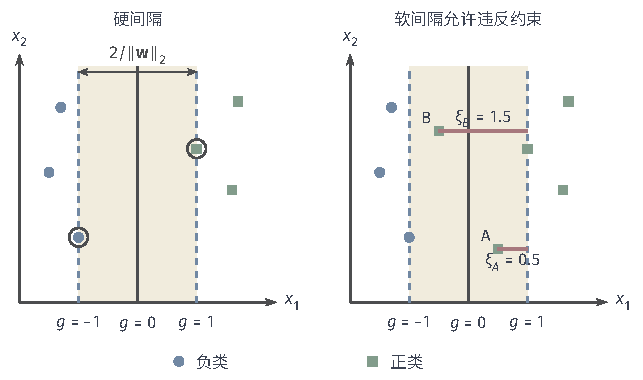
\includegraphics[width=108.850mm]{figures/03-models/01-classic-models/tikz/classification-svm-margin/figure.pdf}
  \caption{硬间隔与软间隔的教学示意，坐标无量纲。蓝圆为负类，赭方为正类；两个面板都给定$\bm{w}=(1,0)^{\top}$、$b=-2$，黑色实线为决策边界$g=0$，蓝色虚线为间隔边界$g=\pm1$。单侧规范间隔为$1/\lVert\bm{w}\rVert_2=1$，两虚线总宽为$2/\lVert\bm{w}\rVert_2=2$；左图圈出间隔上的样本。右图红色线段直接标出松弛量：A位于$x_1=2.5$，正确分类但在间隔内，$\xi_A=0.5$；B位于$x_1=1.5$，已被错分，$\xi_B=1.5$。右图仅说明给定分界面下的最小松弛量，并非优化后的SVM最优解。}
  \label{fig:classification-svm-margin}
\end{figure}

消去$\bm{\xi}$，式\eqref{eq:classification-svm-soft-primal}等价于
\begin{equation}
  \min_{\bm{w},b}\quad
    \frac12\lVert\bm{w}\rVert_2^2
    +\lambda_{\mathrm{s}}\sum_{i=1}^n
       \max\{0,1-y_i g(\bm{x}_i)\}.
  \label{eq:classification-svm-hinge-objective}
\end{equation}
其中$\ell(z)=\max\{0,1-z\}$是\term{合页损失}（hinge loss）：达到目标间隔以后不再奖励更大的得分，间隔不足时线性增加惩罚。它与前面的截断间隔损失不同，错误一侧的损失没有截断，因而保持凸性。这一形式把“最大间隔加违规代价”与“平方范数正则化加经验损失”联系起来。

惩罚参数的数值还依赖损失是求和还是取平均。将式\eqref{eq:classification-svm-hinge-objective}除以$n\lambda_{\mathrm{s}}$，等价目标是平均合页损失加$\lVert\bm{w}\rVert_2^2/(2n\lambda_{\mathrm{s}})$。所以在不同样本量或不同软件约定之间比较超参数时，应先统一归一化方式。较大的$\lambda_{\mathrm{s}}$允许模型付出更大范数来降低训练损失，较小的值更重视范数控制；范数和损失的这种取舍是否适合任务，需要结合数据、表示与验证结果判断。

软间隔的乘子上界来自松弛变量的最优性条件。分别为$1-\xi_i-y_i g(\bm{x}_i)\le0$与$-\xi_i\le0$引入$\alpha_i,\mu_i\ge0$，拉格朗日函数为
\[
  \begin{aligned}
    L={}&\frac12\lVert\bm{w}\rVert_2^2
       +\lambda_{\mathrm{s}}\sum_i\xi_i\\
      &+\sum_i\alpha_i
        \bigl[1-\xi_i-y_i(\bm{w}^{\top}\bm{x}_i+b)\bigr]
       -\sum_i\mu_i\xi_i.
  \end{aligned}
\]
关于$\bm{w},b$的驻点条件仍是式\eqref{eq:classification-svm-stationarity}，关于每个$\xi_i$则要求
\[
  \lambda_{\mathrm{s}}-\alpha_i-\mu_i=0.
\]
结合$\mu_i\ge0$，得到$0\le\alpha_i\le\lambda_{\mathrm{s}}$。取$\bm{w}=\bm{0}$、$b=0$和所有$\xi_i>1$可以严格满足两组不等式，因此不论数据是否可分，Slater条件都成立。消去原始变量后有
\begin{equation}
  \begin{aligned}
    \max_{\bm{\alpha}}\quad&
      \sum_{i=1}^n\alpha_i
       -\frac12\sum_{i,j=1}^n
         \alpha_i\alpha_j y_i y_j
         \bm{x}_i^{\top}\bm{x}_j\\
    \text{s.t.}\quad&
      \sum_{i=1}^n\alpha_i y_i=0,\\
    &0\le\alpha_i\le\lambda_{\mathrm{s}},
      \qquad i=1,\ldots,n.
  \end{aligned}
  \label{eq:classification-svm-soft-dual}
\end{equation}
对偶可行域非空且紧，目标连续，所以对偶最优值可以取得。原始形式同样有最优解；两类非空时，限制目标的水平集可控制$\bm{w}$与$\bm{\xi}$，再由两类约束控制$b$。

软间隔的互补松弛关系多了一组：
\begin{equation}
  \begin{aligned}
    &\alpha_i^{\ast}(m_i^{\ast}-1+\xi_i^{\ast})=0,\\
    &(\lambda_{\mathrm{s}}-\alpha_i^{\ast})\xi_i^{\ast}=0,\\
    &m_i^{\ast}\ge1-\xi_i^{\ast},\qquad \xi_i^{\ast}\ge0.
  \end{aligned}
  \label{eq:classification-svm-soft-kkt}
\end{equation}
联合原始与对偶可行性，可以逐项读出
\begin{equation}
  \begin{aligned}
    \alpha_i^{\ast}=0
      &\ \Longrightarrow\
        \xi_i^{\ast}=0,\quad m_i^{\ast}\ge1,\\
    0<\alpha_i^{\ast}<\lambda_{\mathrm{s}}
      &\ \Longrightarrow\
        \xi_i^{\ast}=0,\quad m_i^{\ast}=1,\\
    \alpha_i^{\ast}=\lambda_{\mathrm{s}}
      &\ \Longrightarrow\
        m_i^{\ast}=1-\xi_i^{\ast}\le1.
  \end{aligned}
  \label{eq:classification-svm-soft-cases}
\end{equation}
边界上的样本可以出现在三种乘子状态中：$\alpha_i^{\ast}=0$允许$m_i^{\ast}=1$，$\alpha_i^{\ast}=\lambda_{\mathrm{s}}$也允许$\xi_i^{\ast}=0$且$m_i^{\ast}=1$。反过来，$m_i^{\ast}>1$必有$\alpha_i^{\ast}=0$，$m_i^{\ast}<1$必有$\alpha_i^{\ast}=\lambda_{\mathrm{s}}$，而$m_i^{\ast}=1$时乘子可以是盒约束中的任意值，只要整体KKT系统成立。达到上界的乘子因此可能对应边界点、间隔内的正确样本或错分样本，需要结合$m_i^{\ast}$才能区分。

范数项依然只对$\bm{w}$严格凸，足以保证最优权重唯一，却不能保证偏置唯一。一个简单反例是两个输入都为零，标签分别为$+1$与$-1$。此时$\bm{w}^{\ast}=\bm{0}$，任意$b\in[-1,1]$都使总合页损失为$2$，因此都最优。该情形也说明，软间隔可能得到常值得分；只有$\bm{w}\ne\bm{0}$时，才可以继续用$1/\lVert\bm{w}\rVert_2$解释规范间隔的几何宽度。

若存在$0<\alpha_k^{\ast}<\lambda_{\mathrm{s}}$的\term{自由支持向量}（free support vector），它既参与决策又未碰到乘子上界，可用$m_k^{\ast}=1$恢复偏置。若没有这种样本，就应使用KKT给出的偏置区间。令$h_i=\sum_j\alpha_j^{\ast}y_j\bm{K}_{j,i}$，则$\alpha_i^{\ast}=0$要求$y_i(h_i+b)\ge1$，$\alpha_i^{\ast}=\lambda_{\mathrm{s}}$要求$y_i(h_i+b)\le1$。正标签的前一条件与负标签的后一条件给出下界，另两种组合给出上界；从两组界的交集中选择一个$b$，才是完整的恢复规则。该区间不一定收缩为单点。

SMO的一元目标与误差公式不变，但可行区间必须同时保证两个乘子都位于盒子内。令$s=y_i y_j$，新的$\alpha_j$区间为
\begin{equation}
  \begin{aligned}
    s=+1:\quad
    L&=\max\{0,\alpha_i^{(t)}+\alpha_j^{(t)}
                    -\lambda_{\mathrm{s}}\},\\
    H&=\min\{\lambda_{\mathrm{s}},
                    \alpha_i^{(t)}+\alpha_j^{(t)}\};\\
    s=-1:\quad
    L&=\max\{0,\alpha_j^{(t)}-\alpha_i^{(t)}\},\\
    H&=\min\{\lambda_{\mathrm{s}},
           \lambda_{\mathrm{s}}+\alpha_j^{(t)}-\alpha_i^{(t)}\}.
  \end{aligned}
  \label{eq:classification-svm-smo-soft-interval}
\end{equation}
这是由盒约束与等式约束共同截出的区间，通常小于$[0,\lambda_{\mathrm{s}}]$。使用式\eqref{eq:classification-svm-smo-update}剪裁并回代即可；当$\eta=0$时，这里的区间总是有限，可以直接比较端点目标。偏置仍按式\eqref{eq:classification-svm-smo-bias}计算，但优先使用更新后满足$0<\alpha_i<\lambda_{\mathrm{s}}$或$0<\alpha_j<\lambda_{\mathrm{s}}$的样本；二者都不自由时，可暂取两个候选偏置的平均，停止时再按全体KKT条件核验。

在可分数据上，足够大的有限惩罚就能使软间隔与硬间隔精确对应。取任意硬间隔最优乘子$\bm{\alpha}^{\mathrm{h}}$，若$\lambda_{\mathrm{s}}>\max_i\alpha_i^{\mathrm{h}}$，则硬间隔原始解连同$\bm{\xi}=\bm{0}$、$\bm{\alpha}^{\mathrm{h}}$和$\mu_i=\lambda_{\mathrm{s}}-\alpha_i^{\mathrm{h}}>0$满足软间隔KKT。由强对偶它也是软间隔最优解，而且正的$\mu_i$迫使所有最优松弛量为零。若数据不可分，则无论把惩罚增大到多少，都不能恢复一个本来就不存在的硬间隔可行解。

\subsubsection{支持非线性分类（核方法）}
\label{sec:classification-svm-kernels}

软间隔调节间隔违反的代价，核化则把同一间隔准则放到特征空间。设$K$为正定核，以核值替代训练样本内积，就能在不显式构造高维坐标的情况下计算对偶与预测。下面推导相应形式及风险界；核技巧、核合法性和常用核分别见第\ref{sec:classic-overview-kernel-trick}节、第\ref{sec:classic-overview-kernel-validity}节和第\ref{sec:classic-overview-common-kernels}节。

将$\bm{w}\in\mathbb{R}^d$换成$\bm{w}\in\mathcal{H}$，将平方范数换成$\lVert\bm{w}\rVert_{\mathcal{H}}^2$，软间隔原始问题的推导仍然成立。更具体地，把任意$\bm{w}$分解为训练特征张成空间内的部分与其正交部分，后者不改变任何训练得分，却只会增加范数。因此最优权重可以限制在有限个训练特征的张成空间中；驻点条件进一步给出$\bm{w}^{\ast}=\sum_i\alpha_i^{\ast}y_i\bm{\phi}(\bm{x}_i)$。核化对偶于是为
\begin{equation}
  \begin{aligned}
    \max_{\bm{\alpha}}\quad&
      \sum_{i=1}^n\alpha_i
       -\frac12\sum_{i,j=1}^n
          \alpha_i\alpha_j y_i y_j
          K(\bm{x}_i,\bm{x}_j)\\
    \text{s.t.}\quad&
      \sum_{i=1}^n\alpha_i y_i=0,\\
    &0\le\alpha_i\le\lambda_{\mathrm{s}},
      \qquad i=1,\ldots,n.
  \end{aligned}
  \label{eq:classification-svm-kernel-dual}
\end{equation}
在映射后严格可分的硬间隔情形，去掉乘子上界即可。新输入的得分与预测为
\begin{equation}
  \begin{aligned}
    g^{\ast}(\bm{x})
      &=\sum_{i\in S}\alpha_i^{\ast}y_i
         K(\bm{x}_i,\bm{x})+b^{\ast},\\
    \hat y(\bm{x})&=\operatorname{sign}(g^{\ast}(\bm{x})).
  \end{aligned}
  \label{eq:classification-svm-kernel-prediction}
\end{equation}
边界在$\mathcal{H}$中仍然是线性的，在原输入空间中则可能是曲线或曲面。SMO也只需把$\bm{K}_{i,j}$换成$K(\bm{x}_i,\bm{x}_j)$；此时$\eta=\lVert\bm{\phi}(\bm{x}_i)-\bm{\phi}(\bm{x}_j)\rVert_{\mathcal{H}}^2\ge0$，前面的区间、零曲率处理与偏置更新都继续适用。

核技巧去掉了对显式特征维数的直接依赖，但没有去掉对样本量的依赖。构建完整Gram矩阵需要$O(n^2)$次核调用，之后还要执行优化迭代；两者合起来才是训练成本。若一次核计算耗时$t_K$，单次预测的主要核计算量是$O(|S|t_K)$。因此，无限维特征可以通过有限次内积运算使用，与“训练成本只由核计算决定”是两回事。

统计分析也可以沿用同一结构。若$K(\bm{x},\bm{x})\le\kappa^2$几乎处处，则$\lVert\bm{\phi}(\bm{x})\rVert_{\mathcal{H}}\le\kappa$；将间隔风险界中的$R$换成$\kappa$、将权重范数换成Hilbert范数即可。控制的是函数范数、间隔与偏置，而不是显式坐标个数。核和超参数若由数据选择，仍需计入相应的选择代价。

\subsubsection{支持多分类}
\label{sec:classification-svm-multiclass}

二分类模型只需判断得分的正负；当候选类别超过两个时，还需要规定多个类别怎样竞争。硬间隔、软间隔和核方法都能作为构件，但组合多个二分类器与直接优化多类间隔会得到不同的训练目标。

现在将标签改为$y_i\in\{1,\ldots,C\}$，其中$C\ge3$，类别索引记为$c$。最直接的推广仍然保留二分类求解器，只改变训练任务的组织方式。\term{一对一}（one-vs-one，OvO）为每对类别$c<c'$训练一个分类器$h_{c,c'}$，仅使用标签为$c$或$c'$的样本，共有$C(C-1)/2$个模型。每个模型在这两个类别之间投一票，预测为
\[
  \hat y(\bm{x})
  =\argmax_{c\in\{1,\ldots,C\}}
     \sum_{c_1<c_2}\mathbb{1}\{h_{c_1,c_2}(\bm{x})=c\}.
\]
其中$c_1,c_2\in\{1,\ldots,C\}$，票数并列时采用预先约定的固定规则，例如选择较小类别编号。不同类别对可能作出不相容的局部判断，投票负责把这些判断汇总成一个输出，并不要求它们对应同一个全局概率模型。

\term{一对其余}（one-vs-rest，OvR）为每个类别$c$构造二分类标签：原标签为$c$时取$+1$，其余取$-1$。训练$C$个实值得分函数$g_c$后，使用
\[
  \hat y(\bm{x})=\argmax_{c\in\{1,\ldots,C\}}g_c(\bm{x}),
\]
并固定平局规则。即使所有得分都为负，或多个类别得分为正，这个最大值规则仍能给出类别。它比较的是独立模型的得分，得分尺度与训练中的类别不平衡可能影响比较，因此通常需要统一预处理、损失约定并评估各类别的错误，若要比较类别后验，还需建立并检验相应的概率映射。

图\ref{fig:classification-svm-multiclass}把四个类别展开成具体训练任务。沿着一列看，一对一中的每个类别只参与三个任务；一对其余中，每个样本都参与四个任务，但只有一个任务把它标为正类。沿着一行看，前者忽略不属于当前类别对的样本，后者把所有其他类别合并为负类。这种训练标签的差异，决定了两个组合器面对的子问题并不相同。

\begin{figure}[htbp]
  \centering
  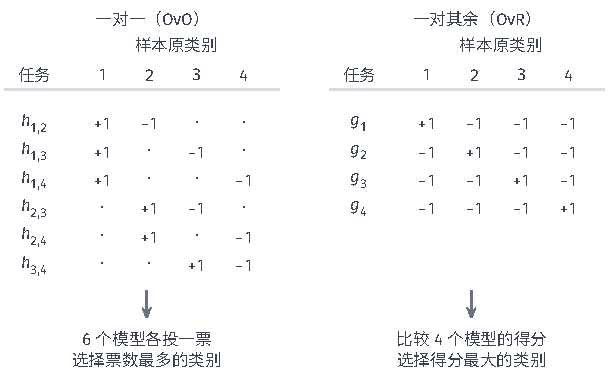
\includegraphics[width=104.027mm]{figures/03-models/01-classic-models/tikz/classification-svm-multiclass/figure.pdf}
  \caption{四分类任务中的两种二分类组合方式。各行对应一个待训练模型，各列对应样本的原类别；$+1$和$-1$是为该任务重新编码的标签，点号表示该类样本不参与训练。一对一训练6个模型并汇总类别选票，一对其余训练4个模型并比较实值得分。图中给出训练与预测规则，不预设两种方法会产生相同的分类结果。}
  \label{fig:classification-svm-multiclass}
\end{figure}

OvO训练$C(C-1)/2$个模型，每个子问题使用两类样本；OvR训练$C$个模型，每个子问题使用全部样本，并面对一个类别与其余类别的数量差异。因此总成本需要结合子问题大小和求解器估计。LIBSVM的多类SVM使用OvO，scikit-learn的核分类器\code{SVC}沿用这一训练方式；输出得分的展示形状还可另行设置。类别较多时，模型存储、支持向量的重复使用与预测核调用量也会影响选择。

如果希望组合器能够容忍若干二分类判断错误，可以为每个类别安排一个彼此分离的编码。\term{纠错输出码}（error-correcting output codes，ECOC）将类别$c$表示成长度为$q$的码字$\bm{M}_{c,:}$，其中码本$\bm{M}\in\{-1,+1\}^{C\times q}$的各行互不相同，每列同时含两种符号。第$j$列定义一个二分类任务，样本$i$的训练标签为$\bm{M}_{y_i,j}$；训练后得到$q$个二分类器$h_j$。预测时形成输出码$\bm{h}(\bm{x})=(h_1(\bm{x}),\ldots,h_q(\bm{x}))$，再选择最近的类别码字：
\begin{equation}
  \begin{aligned}
    \hat y(\bm{x})
      &=\argmin_c d_{\mathrm{H}}
          \bigl(\bm{h}(\bm{x}),\bm{M}_{c,:}\bigr),\\
    d_{\mathrm{H}}(\bm{u},\bm{v})
      &=\sum_{j=1}^q\mathbb{1}\{u_j\ne v_j\}.
  \end{aligned}
  \label{eq:classification-svm-ecoc}
\end{equation}
这里的\term{汉明距离}（Hamming distance）就是两个码字不一致的位置数。要表示$C$个不同类别，至少需要$q\ge\lceil\log_2 C\rceil$；加入冗余位的目的，是增大不同类别之间的距离，而不只是增加分类器个数。Dietterich与Bakiri系统研究了这种将多分类转换为多个编码位学习问题的方法\scite{dietterich1995ecoc}。

纠错能力可以直接证明。记码本最小类间距离为$\Delta_{\min}$，若真实类别为$c$，输出码与$\bm{M}_{c,:}$相差$e$位，则对任意$c'\ne c$，三角不等式给出
\[
  d_{\mathrm{H}}(\bm{h},\bm{M}_{c',:})
  \ge d_{\mathrm{H}}(\bm{M}_{c,:},\bm{M}_{c',:})-e
  \ge\Delta_{\min}-e.
\]
只要$2e<\Delta_{\min}$，真实码字就比任何其他码字更近。因此至多$\lfloor(\Delta_{\min}-1)/2\rfloor$位错误可以被最近码字解码纠正。这个结论以实际错误位数为条件；若多个二分类器因为相同特征缺陷而同时犯错，冗余编码本身并不能保证错误位数足够小。

另一条路线不再训练彼此独立的二分类器，而是直接优化类别之间的竞争关系。\term{Crammer--Singer多类SVM}（Crammer--Singer multiclass SVM）要求真实类别得分至少比每个错误类别高一个单位间隔，从而在同一目标中学习所有类别权重。

令$\bm{W}=[\bm{w}_1,\ldots,\bm{w}_C]\in\mathbb{R}^{d\times C}$，使用带偏置的版本$g_c(\bm{x})=\bm{w}_c^{\top}\bm{x}+b_c$，相应优化问题为\scite{crammer2001multiclass}。
\begin{equation}
  \begin{aligned}
    \min_{\bm{W},\bm{b},\bm{\xi}}\quad&
      \frac12\sum_{c=1}^C\lVert\bm{w}_c\rVert_2^2
       +\lambda_{\mathrm{s}}\sum_{i=1}^n\xi_i\\
    \text{s.t.}\quad&
      g_{y_i}(\bm{x}_i)-g_c(\bm{x}_i)\ge1-\xi_i,
      \quad c\ne y_i,\\
    &\xi_i\ge0,\qquad i=1,\ldots,n.
  \end{aligned}
  \label{eq:classification-svm-crammer-singer}
\end{equation}
不使用偏置时固定$\bm{b}=\bm{0}$；使用偏置时，可加$\sum_c b_c=0$去掉共同平移的不识别性。消去松弛变量后，每个样本的损失为$\max\{0,\max_{c\ne y_i}[1+g_c(\bm{x}_i)-g_{y_i}(\bm{x}_i)]\}$，即惩罚最强错误竞争者超过允许差距的程度。预测仍取$\argmax_c g_c(\bm{x})$，并可将权重推广到核特征空间。

这一联合目标明确比较了类别之间的相对间隔，OvR则分别比较“该类”与“其余类”。二者的约束数、求解器和数据分解方式不同，训练成本与预测质量也要在相同数据和调参预算下评估。联合建模提供了不同的归纳偏好，并不构成相对于OvO或OvR的普遍性能排序。

\subsubsection{小结}
\label{sec:classification-svm-summary}
\label{sec:classification-svm-assessment}

SVM的主要特点是把分类偏好写进一个明确的优化问题：表示由核决定，复杂度由范数限制，训练误差通过间隔损失进入目标。它不要求预先假设完整的类条件分布，能够用于高维特征，并通过支持向量表示保留决定边界的训练信息。文本分类可以先评估稀疏线性模型，手写字符识别可以比较线性与局部非线性核，生物序列任务则可能需要结构化核。这些应用说明可选择的表示丰富，并不意味着某个核在所有场景都有优势。

核SVM的成本分为核计算、优化和预测。通用实现可能需要二次规模的核存储，优化时间取决于工作集策略、缓存、条件数与停止精度，预测成本随支持向量数变化。线性SVM可直接利用稀疏特征和专门求解器。给定任务的样本数、特征结构与预算后，应分别测量内存、训练时间和预测延迟。

输出含义也需要与使用目标一致。$g(\bm{x})$是有符号的分类得分，其绝对值不等于后验概率。需要概率时，可以在未用于拟合该得分函数的校准数据上使用\term{Platt缩放}（Platt scaling），拟合形如
\[
  \widehat p(y=+1\mid\bm{x})
  =\frac1{1+\exp(a_{\mathrm{cal}}g(\bm{x})+b_{\mathrm{cal}})}
\]
的映射；也可以采用\term{保序回归}（isotonic regression），在保持得分顺序的条件下学习非参数的单调概率映射。前者形状受限，后者更灵活但在校准样本较少时可能过拟合，二者都需要独立评估概率质量\scite{niculescu2005probabilities}。

实践中也可用交叉拟合得到样本外得分来训练校准器。校准增加了一层需要数据学习的模型，并不会使原始SVM得分自动成为可靠概率。

回到开头的边界选择问题，SVM给出的答案是：在约定的特征几何中，同时衡量边界的范数与样本的间隔不足。这个答案能够通过凸优化实现，也能在输入有界、范数受限和正确抽样假设下获得统计解释。真正使用时，还需共同选择特征尺度、核参数与$\lambda_{\mathrm{s}}$，并把超参数选择、概率校准和最终测试分开。最大间隔、稀疏表示与核化分别解决不同问题；明确它们的条件，才能判断模型的表达能力、计算成本和泛化表现是否符合当前任务。


\subsection{模型对比与总结}
\label{sec:classification-geometry-summary}

三种基本模型都以线性得分比较类别，权重与阈值的来源却不同。生成式LDA估计类均值、协方差和先验，再用贝叶斯法则形成边界；Fisher判别直接最大化类间散度相对于类内散度的比例。感知机在违反分类条件时更新，可分训练集上的输出是随访问顺序变化的可行分隔面。SVM将间隔写进优化目标，以范数和训练损失的权衡选取解。表\ref{tab:classification-linear-comparison}比较这些依据，后面的扩展分别调节协方差、表示、稀疏化与间隔参数。

\begin{table}[htbp]
  \centering
  \small
  \begin{tabularx}{\linewidth}{@{}>{\RaggedRight\arraybackslash}p{18mm}>{\RaggedRight\arraybackslash}X>{\RaggedRight\arraybackslash}X@{}}
    \toprule
    模型 & 边界由什么决定 & 主要条件与代价 \\
    \midrule
    LDA & 类均值、共享协方差与类先验 & 高斯假设支持概率解释；协方差估计需足够样本或正则化。 \\
    感知机 & 错分样本触发的权重更新 & 正间隔可分性支持有限更新界；不可分时需停止规则或变体。 \\
    线性 SVM & 范数与间隔损失的权衡 & 硬间隔要求可分；软间隔需选择惩罚强度。 \\
    核 SVM & 特征空间中的间隔 & 核定义相似性；训练与预测开销受样本数和支持向量数影响。 \\
    \bottomrule
  \end{tabularx}
  \caption{线性与核化分类器的比较。LDA 一行指共享协方差的高斯生成模型；Fisher 投影本身不要求高斯分布。各模型的理论保证分别针对估计、更新次数或风险，不能直接互换。}
  \label{tab:classification-linear-comparison}
\end{table}

如果不同类别的类内变化方向和尺度明显不同，共享协方差就会限制LDA的表达能力。第\ref{sec:classification-lda-model}节已经定义的二次判别分析（QDA）保留类条件高斯假设，却为每个类别估计独立的协方差矩阵$\hat{\bm{\Sigma}}_c$。删去各类共同的常数项后，其判别得分为
\begin{equation}
  \begin{aligned}
    \delta_c(\bm{x})
      ={}&\log\hat{\pi}_c-\frac12\log\det\hat{\bm{\Sigma}}_c\\
        &-\frac12(\bm{x}-\hat{\bm{\mu}}_c)^\top
          \hat{\bm{\Sigma}}_c^{-1}(\bm{x}-\hat{\bm{\mu}}_c).
  \end{aligned}
  \label{eq:classification-qda-score}
\end{equation}
任意两类得分之差含有关于$\bm{x}$的二次项，所以边界一般是二次曲面。当协方差相同时，二次项相消，又得到 LDA。增加自由度也增加了估计负担：共享协方差模型需要$O(d^2+Cd)$个参数，QDA 则需要$O(Cd^2)$个参数；每一类只有少量样本时，独立协方差容易不稳定甚至奇异。第\ref{sec:classification-gda}节将从生成分布的角度统一这两种模型。

在完全共享与完全独立之间，可以让各类借用一部分合并统计量。\term{正则化判别分析}（regularized discriminant analysis, RDA）通过收缩协方差来控制这种取舍。Friedman 的原始方法包含两个调节方向：将类内协方差向合并协方差收缩，再向球形协方差收缩\scite{friedman1989rda}。
记$n_c$为第$c$类样本数，$\hat{\bm{\Sigma}}$为以$n$为分母的合并协方差。一种与原始构造相符的写法是
\begin{equation}
  \begin{aligned}
    \bm{A}_c(a)
      &=\frac{(1-a)n_c\hat{\bm{\Sigma}}_c+an\hat{\bm{\Sigma}}}
              {(1-a)n_c+an},\\
    \tilde{\bm{\Sigma}}_c(a,b)
      &=(1-b)\bm{A}_c(a)
        +b\,\frac{\operatorname{tr}\bm{A}_c(a)}{d}\bm{I},
        \qquad a,b\in[0,1].
  \end{aligned}
  \label{eq:classification-rda}
\end{equation}
当$b=0$时，$a=0$与$a=1$分别对应 QDA 与 LDA 的协方差估计；增大$b$会减弱各方向方差差异，并在平均方差为正时帮助获得可逆估计。两个参数应在训练集内部通过验证选择。当合并协方差和各类协方差均奇异时，可逆性还需要平均方差为正的球形收缩项或其他正则化。

Fisher 判别还可以沿核方法的路线扩展。Mika 等提出的\term{核 Fisher 判别}（kernel Fisher discriminant, KFD）在特征空间中重新计算类均值与散度，再最大化投影后的类间与类内散度比\scite{mika1999kernel}。
将投影方向写成$\bm{w}=\sum_{i=1}^n a_i\phi(\bm{x}_i)$，即可把目标表达为关于系数$\bm{a}$和核矩阵的广义 Rayleigh 商，并用正则化处理类内散度的奇异性。它与核 SVM 的区别仍在训练准则：KFD 关注整体类统计量，SVM 关注间隔及其违反程度。KFD 的基本解通常没有支持向量式的稀疏性，预测可能需要访问全部训练样本；若要从投影得分得到后验概率，还需额外建立得分分布或校准模型。

除了用间隔约束产生稀疏性，还可以为不同基函数分别学习先验的收缩强度。\term{相关向量机}（relevance vector machine, RVM）采用
\[
  g(\bm{x})=w_0+\sum_{i=1}^n w_i K(\bm{x}_i,\bm{x}),
  \qquad
  p(w_i\mid a_i)=\mathcal{N}(0,a_i^{-1}),
\]
其中$a_i>0$是每个权重各自的先验精度，即先验方差的倒数。分类时再用适当的概率链接函数把$g(\bm{x})$转换为类别概率。RVM通过最大化对权重积分后得到的边缘似然来估计各个精度，部分$a_i$可能趋向无穷，对应权重的分布随之集中到零。在数值实现中，可以按预定的精度或贡献准则剔除相应基函数，使预测只保留一部分训练样本的基函数。有限但很大的精度只造成强收缩，并不自动把权重变成精确的零；这里的稀疏化依赖精度学习及剔除过程。Tipping 系统介绍了这一稀疏贝叶斯学习框架\scite{tipping2001rvm}。
RVM输出模型内的预测分布，其调节对象是基函数及先验精度；精度学习包含非凸优化，分类似然还需要近似推断。相关向量的数量取决于任务与剔除准则，原模型的概率也需要在实际分布上检验校准。

如果希望调参时直接联系间隔错误与支持向量比例，可以考虑\term{$\nu$-SVM}（nu-support vector machine）。它把间隔阈值$\rho\geq0$也作为变量，在目标中用参数$\nu$奖励更大的阈值，同时惩罚平均松弛量：
\begin{equation}
  \begin{aligned}
    \min_{\bm{w},b,\rho,\bm{\xi}}\quad&
      \frac12\lVert\bm{w}\rVert_2^2-\nu\rho
      +\frac1n\sum_{i=1}^n\xi_i\\
    \text{满足}\quad&
      y_i(\bm{w}^{\top}\phi(\bm{x}_i)+b)\geq\rho-\xi_i,\\
    &\xi_i\geq0,\qquad \rho\geq0.
  \end{aligned}
  \label{eq:classification-nu-svm}
\end{equation}
在最优$\rho>0$时，其对偶乘子满足$0\leq\alpha_i\leq1/n$且$\sum_i\alpha_i=\nu$。因此至少需要$\nu n$个非零乘子，而每个严格违反间隔的样本都占用一个达到$1/n$的乘子，于是间隔错误比例不超过$\nu$，支持向量比例不低于$\nu$。这里计数的是训练集上的间隔错误，包括正确分类但落在间隔内的样本\scite{scholkopf2000nu}。

参数范围还受到类别比例约束。由偏置的驻点条件$\sum_i\alpha_i y_i=0$，正负两类的乘子和都为$\nu/2$；若两类样本数分别为$n_+$和$n_-$，盒约束便要求
\[
  0<\nu\leq\nu_{\max}
  :=\frac{2\min(n_+,n_-)}{n}.
\]
这里的上界不只是$\rho>0$解释所需的附加条件。若$\nu>\nu_{\max}$，令$\bm{w}=\bm{0}$、让常数偏置把全部样本判为多数类，并令少数类松弛量等于$2\rho$、多数类松弛量为零，就得到一条满足约束的射线；其目标值为$(\nu_{\max}-\nu)\rho$，随$\rho\to\infty$趋于$-\infty$。因此，虽然约束集合仍非空，优化问题却无界而没有有限最优解。在允许区间内取得有限最优解后，前述比例结论仍以最优$\rho>0$为条件；$\rho=0$时不能直接套用。

协方差收缩控制估计自由度，核化改变可表达的关系，RVM以先验精度及剔除实现稀疏化，$\nu$-SVM把训练间隔比例联系到调节参数。比较这些扩展时，固定特征处理和评价方式，再考察样本能否支持增加的自由度，以及训练、存储和预测成本是否符合用途。
\section{基于邻域的分类}
\label{sec:classification-instances}

$k$-NN分类由查询附近的标签形成类别判断：保存训练实例，按距离找出邻居，再聚合标签。与回归中的响应平均相比，分类采用多数投票或局部类别比例。下面比较邻居权重与原型压缩，并分析局部噪声对风险的影响；近邻表示和检索的基础见第\ref{sec:classic-overview-neighborhood}节，回归对应形式见第\ref{sec:regression-knn}节。

\subsection{$k$近邻分类（$k$-NN）}
\label{sec:classification-knn}

近邻分类的统计目标是学习类别决策，而不只是复现训练标签。Cover与Hart在1967年的论文中回顾了Fix与Hodges始于1951年报告的近邻判别研究：在所研究的条件下，让近邻数随样本量增长、同时让其占比趋于零，可以获得一致性。Cover与Hart则分析了始终只取一个最近邻时，极限错误率与贝叶斯风险之间的界。前者用越来越多的邻居平均标签噪声，后者刻画单个邻居仍保留多少判别信息；两者分别研究增长近邻数与固定单个近邻的渐近风险\scite{coverhart1967}。

\subsubsection{模型结构}
\label{sec:classification-knn-structure}

给定训练集$D_n=\{(\bm{x}_i,y_i)\}_{i=1}^n$、距离$\rho$以及$1\leq k\leq n$，用$N_k(\bm{x})\subseteq\{1,\ldots,n\}$表示查询$\bm{x}$的$k$个最近邻索引。预测规则为
\begin{equation}
  \hat h_{n,k}(\bm{x})
  =\argmax_{c\in\{1,\ldots,C\}}
  \sum_{i\in N_k(\bm{x})}\mathbb{1}\{y_i=c\}.
  \label{eq:classification-knn-vote}
\end{equation}
距离相同时，按预先约定、独立于标签的顺序选取邻居；类别票数并列时也使用固定规则。多分类在奇数$k$时也可能出现票数并列，因此两种平局都需要明确规则。

式\eqref{eq:classification-knn-vote}也可以理解为估计查询附近的类别比例：
\begin{equation}
  \hat\eta_{n,c}(\bm{x})
  =\frac{1}{k}\sum_{i\in N_k(\bm{x})}\mathbb{1}\{y_i=c\},
  \qquad
  \hat h_{n,k}(\bm{x})=\argmax_c\hat\eta_{n,c}(\bm{x}).
  \label{eq:classification-knn-posterior}
\end{equation}
比例估计解释了投票为什么可能有效：若邻域内的条件类别分布变化不大，邻居标签就能提供关于当前输入的统计证据。局部比例的误差取决于邻域大小与标签噪声，概率质量需通过样本外数据检验。

图~\ref{fig:classification-knn-neighborhood}固定训练点和查询，只改变参与投票的近邻数。取查询$\bm{x}=(0,0)$，样本1、3、4、6属于类1，其余样本属于类2。按欧氏距离计算，七个样本到查询的平方距离依编号为$1,2,2.5,4.25,5,9,10.25$，因此编号也表示由近到远的次序。

$k=1$时只有样本1投票，查询被判为类1；$k=5$时样本1至5投票，其中类1有三票、类2有两票，预测仍为类1。两幅图中的圆分别经过第1和第5个邻居，半径为$1$和$\sqrt5$。圆表示当前查询的证据范围，整个平面上的分类边界则由各查询的投票共同决定。比较两个$k$的准确性还需要查询的真实标签。

\begin{figure}[htbp]
  \centering
  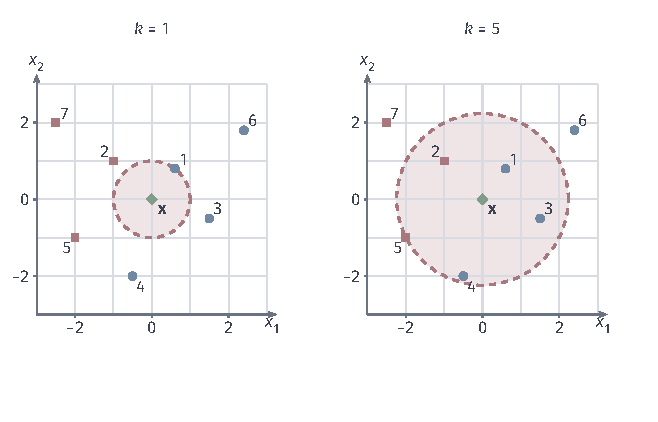
\includegraphics[width=111.404mm]{figures/03-models/01-classic-models/tikz/classification-knn-neighborhood/figure.pdf}
  \caption{同一查询下的近邻范围与投票变化。教学构造取$n=7$、$d=2$、无量纲坐标和欧氏距离，查询为$\bm{x}=(0,0)$；两图的样本、编号及坐标尺度完全相同。蓝色圆点表示类1，红色方点表示类2，绿色菱形表示查询，红色虚线圆表示包含边界的近邻范围。左图$k=1$、半径$1$，蓝、红票数为$1:0$；右图$k=5$、半径$\sqrt5$，票数为$3:2$，因此判为蓝色类。各邻居等权投票，距离和票数均无并列；点的位置、标签与参数均为人为设定，不代表真实数据实验。}
  \label{fig:classification-knn-neighborhood}
\end{figure}

\subsubsection{参数学习}
\label{sec:classification-knn-learning}

基本$k$-NN分类没有固定维数参数的优化过程，但需要确定输入表示、距离、近邻数及检索方式。“非参数化”是指预测关系不局限于一个固定有限维参数族；它仍有超参数，预处理和模型选择也属于学习。

距离决定哪些样本会参与投票。对数值特征，欧氏距离$\rho(\bm{x},\bm{z})=\lVert\bm{x}-\bm{z}\rVert_2$容易计算，却会放大数值范围较大的坐标。收入和年龄共同作为特征时，直接使用原始单位会让收入差异主导距离。标准化、按业务意义设定尺度或学习特征权重都可改变这一点；不同特征的重要性可通过任务知识或训练数据确定。标准化参数只能从训练集估计，交叉验证时应在各训练折内重新拟合，避免验证信息提前进入距离。

类别型特征可采用\term{汉明距离}（Hamming distance），按不同取值的坐标数比较，而不能把任意类别编码的数字差当成有意义的远近。文本的TF--IDF等稀疏向量常比较余弦相似度，强调方向而非长度；$1$减余弦相似度一般不满足三角不等式，不能直接套用所有度量空间结论。对非零向量作单位长度归一化后，按余弦相似度排序与按欧氏距离排序等价，此时可用欧氏空间中的解释。

若特征之间相关，可以考虑\term{马氏距离}（Mahalanobis distance），用协方差调整方向上的尺度：
\begin{equation}
  \rho_{\mathrm{M}}(\bm{x},\bm{z})^2
  =(\bm{x}-\bm{z})^\top
   \bm{\Sigma}^{-1}(\bm{x}-\bm{z}),
  \label{eq:classification-mahalanobis}
\end{equation}
其中$\bm{\Sigma}\in\mathbb{R}^{d\times d}$须正定。样本不足时协方差估计可能奇异，需要正则化；整体协方差也不一定符合分类所需的相似性。\term{度量学习}（metric learning）进一步利用标签选择距离，\term{大间隔最近邻}（large margin nearest neighbor, LMNN）是其中一种方法\scite{weinberger2009}。它学习线性变换，拉近同类目标邻居，并用间隔约束排开异类样本。

另一种选择是\term{近邻成分分析}（neighbourhood components analysis, NCA），它对邻居选择作概率化处理，通过提高留一预测中选到同类样本的概率学习线性变换。与只调整每个坐标尺度相比，这类方法还能改变坐标间的组合，但也引入额外训练目标和过拟合风险。学得的度量需要与$k$一起在未参与拟合的数据上评价，以检验监督变换是否保留了新样本的类别关系\scite{goldberger2004nca}。

近邻数$k$控制局部平均的范围。$k=1$时，一个错误标签就会影响邻近查询；增加邻居可平均这类波动，也会混入更远区域并削弱局部细节。因此$k$的选择需要结合类别比例、局部密度与距离表示，在训练集内部验证。$k\approx\sqrt n$可以作为搜索起点，最终选择依据相同评价条件下的误差。

检索代价需要区分距离计算与邻居选择。对一个$d$维稠密查询，朴素扫描$n$个训练样本计算距离需$O(nd)$；若再把所有距离排序，总代价为$O(nd+n\log n)$。采用线性选择算法得到最小的$k$项，再作投票，可达$O(nd+n+k)$；使用大小为$k$的堆则需$O(nd+n\log(k+1)+k)$。因此，通常所说的$O(nd)$朴素预测复杂度隐含了无需完整排序的选择方法。训练集的存储为$O(nd)$，批量计算、硬件、精度要求和延迟预算共同决定这种实现的可用规模。

KD树或球树（ball tree）等精确索引通过空间划分排除不可能更近的样本。低维且分布有利时，它们可以减少访问量；最坏情形仍会检查大部分样本。索引保留原预测规则，选择时比较建索引成本、内存和实际查询时间，维数的影响需结合数据分布测量。

对高维大规模数据，还可以用\term{近似最近邻检索}（approximate nearest-neighbor search）交换少量检索误差与计算收益。局部敏感哈希（locality-sensitive hashing, LSH）让相近向量较可能进入同一哈希桶；分层可导航小世界图（hierarchical navigable small world, HNSW）沿多层邻接图逐步寻找候选；倒排文件与乘积量化（inverted file with product quantization, IVF--PQ）先缩小候选分区，再用压缩编码近似距离。这些方法的搜索预算和压缩程度会改变邻居集合，需同时检查邻居召回率与最终分类误差。以下理论以精确检索为前提，不直接覆盖任意近似索引。

\subsubsection{理论分析}
\label{sec:classification-knn-theory}

基本$k$-NN的预测在给定距离与近邻数后直接计算，无须迭代拟合一组参数。下面的统计问题是：样本量增加时，邻居位置怎样变化，局部类别比例怎样估计条件概率，所得分类器的风险怎样接近贝叶斯风险。

位置接近仍可能伴随标签差异。两个相同输入在类别重叠或标签噪声下，也可独立产生不同标签。因此先规定训练集、查询与标签的随机性，再将邻居位置的极限联系到条件类别分布和分类风险。

设训练样本与测试点$(\bm{X},Y)$独立同分布于$\mathbb{R}^d\times\{1,\ldots,C\}$，$P_X$为输入边缘分布，$C\geq2$。令
\begin{equation}
  \eta_c(\bm{x})=\mathbb{P}(Y=c\mid\bm{X}=\bm{x}),
  \qquad
  r^\ast(\bm{x})=1-\max_c\eta_c(\bm{x}).
  \label{eq:classification-local-bayes-risk}
\end{equation}
选择后验概率最大的类别达到条件最小错误率$r^\ast(\bm{x})$，对输入平均得到\term{贝叶斯风险}（Bayes risk）$R^\ast=\mathbb{E}_{\bm{X}}r^\ast(\bm{X})$。给定一份训练集的测试风险，与再对训练集平均的风险分别记为
\begin{align}
  L_{n,k}(D_n)
  &=\mathbb{P}\{\hat h_{n,k}(\bm{X})\neq Y\mid D_n\},
  \label{eq:classification-knn-conditional-risk}\\
  R_{n,k}&=\mathbb{E}_{D_n}L_{n,k}(D_n).
  \label{eq:classification-knn-expected-risk}
\end{align}
若打破距离并列采用独立随机化，以上期望同时包含该随机化。下面的Cover--Hart界针对$R_{n,1}$的极限，不是任意有限$n$的风险上界，也不是每份训练集条件风险的逐一保证。

\paragraph{表达能力}
近邻分类通过局部标签比例决定类别，距离和邻域规模限定局部性。足够密的代表性样本可支持细边界，但固定有限样本、错误尺度或无关特征可能使局部多数偏离目标。

\paragraph{收敛性}
标准$k$-NN保存训练实例，给定距离和邻居数后没有参数优化过程，也就没有迭代找到最优参数的保证或速率。精确检索与投票能直接执行已定义的预测规则；朴素稠密实现为每个查询计算$n$个距离，约需$O(nd)$运算，再选择近邻。近似检索降低计算成本时，漏检或错检造成的误差必须另行评价。

\paragraph{泛化性}
先说明足以支撑极限计算的一组分布条件。使用固定的欧氏距离，精确寻找最近邻，邻居选择不依赖标签；对$P_X$几乎处处的非原子点$\bm{x}$，各$\eta_c$在该点相对于$P_X$的支撑集连续。所谓原子点是$P_X(\{\bm{x}\})>0$的点，它不需要这里的连续性要求。该条件不要求输入分布有密度，更不要求每个欧氏空间位置都有正密度，但它也不只是“条件概率存在”。

\begin{lemma}[最近邻风险的极限]
  \label{lem:classification-nearest-neighbor-limit}
  在上述抽样、检索与连续性条件下，最近邻位置几乎必然趋于查询位置，并且
  \begin{equation}
    R_{1,\infty}:=\lim_{n\to\infty}R_{n,1}
    =\mathbb{E}_{\bm{X}}\left[
      1-\sum_{c=1}^{C}\eta_c(\bm{X})^2
    \right].
    \label{eq:classification-nearest-neighbor-limit}
  \end{equation}
\end{lemma}

\begin{proof}
  将训练集看作同一无穷独立样本序列的前$n$项。固定支撑集中的查询$\bm{x}$，用$I_n$表示最近邻索引，用$B(\bm{x},\varepsilon)$表示半径$\varepsilon>0$的开球。支撑集的定义保证该球有正概率，因此
  \[
    \mathbb{P}\{\|\bm{X}_{I_n}-\bm{x}\|_2\geq\varepsilon\}
    =\bigl[1-P_X(B(\bm{x},\varepsilon))\bigr]^n
    \longrightarrow0.
  \]
  最近邻距离随$n$不增，对$\varepsilon=1,1/2,1/3,\ldots$分别取极限，即得$\bm{X}_{I_n}\to\bm{x}$几乎必然成立。欧氏空间具有可数拓扑基，不在支撑集中的点可被可数个零概率开集覆盖，故支撑集本身具有$P_X$概率1。若$\bm{x}$为原子点，训练序列几乎必然在有限步后出现$\bm{x}$，此后最近邻距离一直为零。

  对非原子点，由连续性得到$\eta_c(\bm{X}_{I_n})\to\eta_c(\bm{x})$；对原子点，这个等式最终直接成立。最近邻索引只依赖输入及与标签独立的平局约定。给定查询和所有训练输入后，测试标签与选中的训练标签独立，选中标签属于$c$的概率为$\eta_c(\bm{X}_{I_n})$。故对训练集平均的条件错误率为
  \[
    r_n(\bm{x})
    =1-\sum_{c=1}^{C}\eta_c(\bm{x})
       \mathbb{E}\bigl[\eta_c(\bm{X}_{I_n})\bigr],
  \]
  这里的期望针对固定查询时的训练输入及邻居选择随机性。由于后验概率有界，可用支配收敛定理得到
  \[
    r_n(\bm{x})\longrightarrow
    r_\infty(\bm{x})
    :=1-\sum_{c=1}^{C}\eta_c(\bm{x})^2.
  \]
  再利用$0\leq r_n(\bm{x})\leq1$，对$\bm{x}$积分并交换极限与期望，就得到式\eqref{eq:classification-nearest-neighbor-limit}。
\end{proof}

极限中的平方项来自两次独立的类别抽取，而不是说最近邻标签本身几乎必然收敛。位置接近保证的是选中标签的条件分布接近查询的条件分布，单次标签抽样的波动仍然存在。

要平均掉这部分噪声，需要让参与投票的邻居数增加；要避免把远处结构混入，又需要邻居只占全部训练样本的越来越小一部分。令$k=k_n$满足$k_n\to\infty$且$k_n/n\to0$。Stone的非参数一致性结果在固定有限维欧氏空间中建立了近邻条件概率估计的积分收敛，也就是对训练集与查询取平均后，估计的绝对误差趋于零；这为后面的风险分析提供了依据\scite{stone1977consistent}。

对精确欧氏近邻，距离并列时可按与数据独立的随机排列选取，类别票数并列时按固定类别顺序决定。对每个$c$，这样的近邻估计满足
\begin{equation}
  \mathbb{E}_{D_n,\bm{X}}
  \bigl|\hat\eta_{n,c}(\bm{X})-\eta_c(\bm{X})\bigr|
  \longrightarrow0.
  \label{eq:classification-knn-posterior-consistency}
\end{equation}
这一结论对$\mathbb{R}^d$上任意固定联合分布成立，不需要前面为简化Cover--Hart证明而采用的逐点连续性条件。其一般证明使用欧氏空间的覆盖性质，不能只用一句普通大数定律代替，因为邻居样本是根据查询和输入位置选择出来的。

在前述连续性条件下，可以直接看出式\eqref{eq:classification-knn-posterior-consistency}的两个来源。给定训练输入，记
\[
  \bar\eta_{n,c}(\bm{x})
  =\frac{1}{k_n}\sum_{i\in N_{k_n}(\bm{x})}\eta_c(\bm{X}_i).
\]
邻居标签在给定输入后独立，所以
\[
  \mathbb{E}\!\left[
    |\hat\eta_{n,c}(\bm{x})-\bar\eta_{n,c}(\bm{x})|
    \,\middle|\,\bm{X}_1,\ldots,\bm{X}_n
  \right]\leq\frac{1}{2\sqrt{k_n}}.
\]
上界来自Bernoulli变量的方差不超过$1/4$及Cauchy--Schwarz不等式。它控制标签抽样波动。对任意有正概率的查询邻域，落入其中的样本比例几乎必然趋向该邻域的概率；由于$k_n/n\to0$，最终会有至少$k_n$个训练样本落入其中。因此，第$k_n$个邻居的距离趋于零。后验连续时，$\bar\eta_{n,c}(\bm{x})-\eta_c(\bm{x})$趋于零；在原子点，最终选中的$k_n$个输入都可等于该点。结合有界性与支配收敛，就得到这组较强正则性条件下的积分收敛。Stone的结论把同一估计分析扩展到了不连续后验。

已有的极限计算还需要与最优分类错误比较，才能说明近邻规则的预测保证。固定$k=1$时，Cover--Hart定理比较引理~\ref{lem:classification-nearest-neighbor-limit}中的极限局部错误与最优局部错误；让$k_n$增长时，则可用式\eqref{eq:classification-knn-posterior-consistency}控制相对于贝叶斯决策多出的错误。这两种风险保证都对训练集和独立测试点取平均。

\begin{theorem}[Cover--Hart界：二分类]
  \label{thm:classification-cover-hart-binary}
  在引理~\ref{lem:classification-nearest-neighbor-limit}的条件下，若$C=2$，则
  \begin{equation}
    R^\ast\leq R_{1,\infty}
    \leq2R^\ast(1-R^\ast)\leq2R^\ast.
    \label{eq:classification-cover-hart-binary}
  \end{equation}
\end{theorem}

\begin{proof}
  固定$\bm{x}$，记$p=\eta_1(\bm{x})$，则$\eta_2(\bm{x})=1-p$，$r^\ast(\bm{x})=\min(p,1-p)$。引理给出
  \begin{align*}
    r_\infty(\bm{x})
    &=1-p^2-(1-p)^2\\
    &=2p(1-p)\\
    &=2r^\ast(\bm{x})\bigl[1-r^\ast(\bm{x})\bigr].
  \end{align*}
  由于$0\leq r^\ast(\bm{x})\leq1/2$，有$2(1-r^\ast(\bm{x}))\geq1$，所以$r_\infty(\bm{x})\geq r^\ast(\bm{x})$。对输入取期望得到下界。对于上界，
  \begin{align*}
    R_{1,\infty}
    &=2R^\ast-2\mathbb{E}_{\bm{X}}[r^\ast(\bm{X})^2]\\
    &\leq2R^\ast-2(R^\ast)^2\\
    &=2R^\ast(1-R^\ast).
  \end{align*}
  不等式利用$\mathbb{E}[Z^2]\geq(\mathbb{E}Z)^2$，也就是对凹函数$2z(1-z)$使用Jensen不等式。再用$1-R^\ast\leq1$得到两倍上界。
\end{proof}

多分类时，不能沿用二类的精确表达式$2p(1-p)$，因为非最大类别的概率还可以在多个类别之间分配。需要控制的是：固定最大后验概率以后，其余类别的概率平方和最小能是多少。

\begin{theorem}[Cover--Hart界：多分类]
  \label{thm:classification-cover-hart-multiclass}
  在引理~\ref{lem:classification-nearest-neighbor-limit}的条件下，对任意有限$C\geq2$，
  \begin{equation}
    R^\ast\leq R_{1,\infty}
    \leq R^\ast\left(2-\frac{C}{C-1}R^\ast\right)
    \leq2R^\ast.
    \label{eq:classification-cover-hart-multiclass}
  \end{equation}
\end{theorem}

\begin{proof}
  固定$\bm{x}$并简记$r=r^\ast(\bm{x})$。取$c^\ast$使$\eta_{c^\ast}(\bm{x})=1-r$，其余$C-1$类的概率之和为$r$。由Cauchy--Schwarz不等式，
  \[
    r^2
    =\left(\sum_{c\neq c^\ast}\eta_c(\bm{x})\right)^2
    \leq(C-1)\sum_{c\neq c^\ast}\eta_c(\bm{x})^2.
  \]
  因而
  \begin{align*}
    \sum_{c=1}^{C}\eta_c(\bm{x})^2
    &\geq(1-r)^2+\frac{r^2}{C-1},\\
    r_\infty(\bm{x})
    &\leq1-(1-r)^2-\frac{r^2}{C-1}\\
    &=2r-\frac{C}{C-1}r^2.
  \end{align*}
  这一步的等号在其余类别的概率都等于$r/(C-1)$时成立。记$g_C(r)=2r-Cr^2/(C-1)$，它在$0\leq r\leq1-1/C$上为凹函数。对输入取期望并用Jensen不等式，
  \[
    R_{1,\infty}
    \leq\mathbb{E}_{\bm{X}}g_C(r^\ast(\bm{X}))
    \leq g_C(R^\ast).
  \]
  去掉非负的二次项得到$R_{1,\infty}\leq2R^\ast$。另一方面，$\eta_c(\bm{x})\leq1-r$，故
  \[
    \sum_{c=1}^{C}\eta_c(\bm{x})^2
    \leq(1-r)\sum_{c=1}^{C}\eta_c(\bm{x})=1-r.
  \]
  于是$r_\infty(\bm{x})\geq r$，积分后得到$R_{1,\infty}\geq R^\ast$。
\end{proof}

这两个界不要求某个参数化类别分布，却仍依赖已列出的抽样和分布正则性条件。若$R^\ast=0$，界给出1-NN的期望风险趋于零；若后验概率在所有位置都为$(0.8,0.2)$，则$R^\ast=0.2$而$R_{1,\infty}=0.32$。后一个教学计算表明，单个近邻即使位于查询附近，也仍带有一次标签抽样的噪声，因此1-NN一般不能使期望风险趋于贝叶斯风险。

\term{贝叶斯一致性}（Bayes consistency）要求期望测试风险趋向贝叶斯风险。对于满足$k_n\to\infty$且$k_n/n\to0$的近邻规则，后验估计的积分收敛已经成立；从后验估计到分类风险，还需要明确的一步。对固定查询和训练集，令$c^\ast$为真实后验最大的类别，$\hat c=\hat h_{n,k_n}(\bm{x})$。由于$\hat\eta_{n,\hat c}\geq\hat\eta_{n,c^\ast}$，
\begin{align*}
  \eta_{c^\ast}(\bm{x})-\eta_{\hat c}(\bm{x})
  &\leq|\eta_{c^\ast}(\bm{x})-\hat\eta_{n,c^\ast}(\bm{x})|\\
  &\quad+|\hat\eta_{n,\hat c}(\bm{x})-\eta_{\hat c}(\bm{x})|\\
  &\leq2\sum_{c=1}^{C}
    |\hat\eta_{n,c}(\bm{x})-\eta_c(\bm{x})|.
\end{align*}
左侧就是相对于贝叶斯决策多出的条件错误率。对训练集与测试输入取期望，再使用式\eqref{eq:classification-knn-posterior-consistency}和类别数有限，得到
\begin{equation}
  R_{n,k_n}\longrightarrow R^\ast,
  \qquad k_n\to\infty,\quad k_n/n\to0.
  \label{eq:classification-knn-bayes-consistency}
\end{equation}

这里对训练集和查询平均，得到风险期望收敛。由于$L_{n,k_n}(D_n)-R^\ast\geq0$，还可推出条件风险依概率趋于$R^\ast$。几乎必然收敛、逐点标签稳定等更强结论需要另外的条件与论证；后验平局时，不同标签本就可能具有相同的最小风险。

\subsubsection{小结}
\label{sec:classification-knn-summary}

$k$-NN将分类组织为表示、距离、检索和局部投票。多分类可以直接投票，密集实例能够表达局部边界；在固定有限维欧氏空间、精确检索与适当增长的近邻数等条件下，前述理论给出期望风险一致性。有限样本精度、学习度量和近似检索造成的误差仍需按实际流程评价。

高维输入可能使局部区域缺少样本，无关坐标也会削弱距离中的类别信息。某些分布的成对距离相对差异会随维数集中变小，影响程度同时取决于内在维数、相关结构与表示。文本分类、推荐、图像检索和异常检测都可使用近邻计算；具体输出可以是类别、检索结果或分数，需要将对应质量与检索成本一起评价。

\subsection{模型对比与总结}
\label{sec:classification-instances-comparison}

基本$k$-NN保存全部训练实例并等权投票。改变权重可调节邻居的影响，学习少量原型则可减少存储和查询量，两者也可结合。原型方法将部分计算移到训练阶段，下面以距离加权、LVQ和最近质心分别说明这些取舍。

当较远邻居会稀释近处证据时，\term{加权$k$近邻}（weighted $k$-nearest neighbors）让不同邻居贡献不同票数：
\begin{equation}
  \hat h(\bm{x})=\argmax_c
  \sum_{i\in N_k(\bm{x})}
  w_i(\bm{x})\mathbb{1}\{y_i=c\},
  \qquad w_i(\bm{x})\geq0.
  \label{eq:classification-weighted-knn}
\end{equation}
至少需要一个权重为正。Dudani在1976年研究了按邻居距离范围作线性缩放的加权方案，使最近邻具有最大权重、较远邻居的权重逐渐减小\scite{dudani1976weighted}。

具体地，把邻居按距离排序为$\delta_1\leq\cdots\leq\delta_k$，第$r$个邻居的权重取
\begin{equation}
  w_r=
  \begin{cases}
    \dfrac{\delta_k-\delta_r}{\delta_k-\delta_1},
      & \delta_k>\delta_1,\\[4pt]
    1, & \delta_k=\delta_1.
  \end{cases}
  \label{eq:classification-dudani-weights}
\end{equation}
另一类常用选择是逆距离权重或高斯形权重$\exp(-\delta_r^2/(2h^2))$，其中$h>0$控制衰减尺度。逆距离形式遇到零距离必须处理，例如只在零距离样本中投票，避免除零。距离加权可能减少远邻干扰，但也可能放大近处噪声；加权后的硬类别输出仍在最大票数类别变化时跳变，其对$k$的敏感程度需要另行评价。其一致性还依赖权重不能长期集中在有限个带噪声邻居上。

若主要困难是存储全部样本，可以转向\term{学习向量量化}（learning vector quantization, LVQ），用监督训练获得少量带类别的\term{原型向量}（prototype vector）。原型是可移动的代表点，不必等于任何一条训练记录。Kohonen发展的LVQ方法为每个类别配置一个或多个原型，查询时只对这些原型作最近邻比较；它保留局部距离判别的形式，但把模型规模转为可控制的原型数量\scite{kohonen2001som}。

以基本LVQ1为例，设原型为$\bm{m}_r\in\mathbb{R}^d$，类别标签为$a_r$，$r=1,\ldots,q$。可从各类训练样本初始化原型。每次读入$(\bm{x}_i,y_i)$，找到最近原型$r^\ast$，只更新它：
\begin{equation}
  \bm{m}_{r^\ast}^{(t+1)}
  =\bm{m}_{r^\ast}^{(t)}
   +\gamma_t s_i
    \bigl(\bm{x}_i-\bm{m}_{r^\ast}^{(t)}\bigr),
  \label{eq:classification-lvq-update}
\end{equation}
其中学习率$\gamma_t>0$通常随训练减小；若$a_{r^\ast}=y_i$，取$s_i=1$把原型拉近，否则取$s_i=-1$把原型推远。其余原型不动。反复遍历样本后，在验证集上选择原型数、学习率和停止时机，预测时输出最近原型的类别标签。

当$q\ll n$时，LVQ的原型存储和朴素查询代价为$O(qd)$。节省程度取决于原型数，而表示能力取决于这些原型是否覆盖分离的类内区域。基本吸引与排斥更新属于启发式训练，结果受初始化和访问顺序影响；其风险分析需要针对这一固定原型模型建立。

将每类限制为一个代表点，并直接取该类样本均值，就得到\term{最近质心分类器}（nearest centroid classifier）。它与LVQ共同使用原型距离，但不需要通过吸引与排斥来训练。令$n_c=\sum_{i=1}^n\mathbb{1}\{y_i=c\}>0$，则
\begin{align}
  \bm{\mu}_c&=\frac{1}{n_c}\sum_{i:y_i=c}\bm{x}_i,
  \label{eq:classification-centroid}\\
  \hat h(\bm{x})&=\argmin_c\|\bm{x}-\bm{\mu}_c\|_2^2.
  \label{eq:classification-nearest-centroid}
\end{align}
预测是在全部$C$个类原型中作一次最近邻选择。训练计算均值需$O(nd)$，存储和单次查询需$O(Cd)$。

第\ref{sec:clustering-kmeans}节的K-means也用均值作为质心，但还要在没有类别标签时估计簇分配；最近质心分类器直接按已知类别分组计算均值，目标是预测预设类别。相同的质心计算因标签条件不同而承担不同任务。

最近质心的两个类别区域由两质心的等距面分开，所以欧氏距离下的两类边界是超平面。若真实类条件分布为具有共同球形协方差的高斯分布、先验概率又相等，用真实均值作最近质心决策就是贝叶斯规则；一般应用可用验证数据检验其误差。类别多峰、尺度差异很大或均值被异常值牵动时，一个质心会丢失重要的几何结构。

在文本分类中，类质心方法常与Rocchio联系起来。Rocchio于1971年研究的相关反馈通过相关与不相关文档调整查询向量，后来的Rocchio分类把类别的文档均值作为原型，将这一思想用于没有查询向量的类别判别。文本表示还可以对文档及原型作归一化，改用余弦相似度，所得分类边界需按具体归一化方式理解\scite{manning2008ir}。

等权近邻保留训练实例，加权近邻调节局部证据，LVQ与最近质心用代表点换取存储和查询效率。原型压缩使预测成本由原型数控制，也加强了对类内几何形态的限制。评价时共同检查距离中的类别信息、原型覆盖和独立测试误差。
\section{基于树与规则的分类}
\label{sec:classification-trees}

沿用第\ref{sec:classic-overview-tree-rules}节的条件分支，分类树在叶节点输出类别或类别比例。以下比较分类任务怎样选择分裂、控制生长并确定叶输出；原始结构之外的规则学习则放在同一节中，便于对照条件共享、覆盖与冲突处理。

沿用训练集$D_n=\{(\bm{x}_i,y_i)\}_{i=1}^n$，其中输入有$d$个特征，$y_i\in\{1,\ldots,C\}$。本节允许特征是数值型或类别型，用$D\subseteq D_n$表示到达某个节点的训练样本。建树需要同时确定测试特征、阈值或取值分组，以及叶节点的输出，并非只估计一组预先固定的数值参数。常见做法是在当前节点选择一个能改善类别划分的测试，再递归处理各个子集；为避免把偶然差异也变成分支，还要限制生长或在生长后\term{剪枝}（pruning），即删除缺少预测收益的子树。

图~\ref{fig:classification-tree-partition}把同一个分类器分别画成区域和条件树。在$[0,1]^2$内，$x_1\leq0.5$的输入直接判为类1；其余输入继续检查$x_2$，不超过$0.55$时判为类2，否则判为类1。左图的水平分界只出现在右半区域，正对应右图中第二次测试只对第一个条件不成立的输入执行。这说明树中的路径不仅记录有哪些条件，也规定条件在哪个区域生效。

\begin{figure}[htbp]
  \centering
  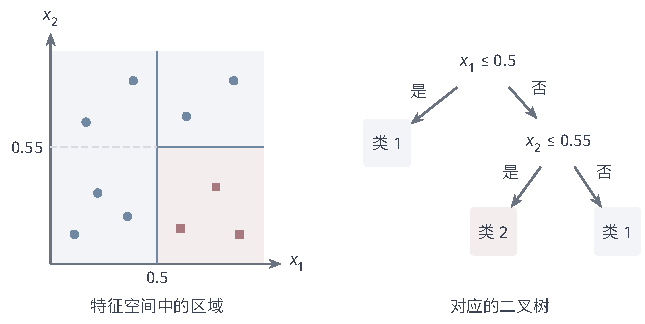
\includegraphics[width=109.241mm]{figures/03-models/01-classic-models/tikz/classification-tree-partition/figure.pdf}
  \caption{二维分类的教学构造。左图为归一化特征空间$[0,1]^2$中的区域划分，圆点表示类1，方点表示类2；右图为产生同一划分的条件树。根节点检查$x_1\leq0.5$，仅在其“否”分支上继续检查$x_2\leq0.55$。点的位置与分裂阈值均为人为设定，不代表真实数据实验。}
  \label{fig:classification-tree-partition}
\end{figure}

不同树算法的主要差异落在三个问题上：怎样评价一次分裂，允许什么样的分支结构，怎样控制树的大小。ID3提供了信息增益驱动的基本构造，C4.5扩展其评分和数据处理方式；CART则采用统一的二叉划分与子树选择框架，形成了另一条决策树研究路线。

\subsection{ID3}
\label{sec:classification-id3}

要决定先检查哪个特征，需要比较“检查前还分不清多少类别”和“检查后还分不清多少类别”。ID3（Iterative Dichotomiser 3）据此选择特征，再在各分支上重复同一过程。Quinlan在1986年的论文中将ID3追溯到Hunt等人的概念学习系统（Concept Learning System, CLS）：CLS向前考察若干层候选树，按测量与误分类代价选择测试；ID3则改用信息驱动的局部评价。这一变化把建树中的“先测什么”落实为当前节点上可计算的信息增益比较，优化范围限定在当前节点的候选测试。本节采用以离散特征、信息增益和不作后剪枝为设定的基本ID3\scite{quinlan1986trees}。

\subsubsection{模型结构}
\label{sec:classification-id3-structure}

在节点样本集$D$上，记$p_c(D)$为类别$c$的样本比例。\term{熵}（entropy）用一个数概括类别分布的不确定性：节点只含一类时为零，各类越均匀，熵越大。采用以2为底的对数，
\begin{equation}
  H(D)=-\sum_{c=1}^{C}p_c(D)\log_2 p_c(D),
  \label{eq:classification-entropy}
\end{equation}
其中约定$0\log_2 0=0$。对第$j$个离散特征，令$V_j$为其可能取值集合，$D_{j,v}=\{(\bm{x}_i,y_i)\in D:x_{i,j}=v\}$。该特征的\term{信息增益}（information gain）是分裂前后熵的减少量：
\begin{equation}
  \operatorname{Gain}(D,j)
  =H(D)-\sum_{v\in V_j}\frac{|D_{j,v}|}{|D|}H(D_{j,v}).
  \label{eq:classification-information-gain}
\end{equation}
空子集对求和的贡献定义为零。这里必须按子集大小加权，否则只有一个样本的小分支会与包含大部分样本的分支同样重要。

ID3用选中的特征建立一个内部节点，每个取值对应一个分支。叶节点保存到达该处的类别计数，并通常输出多数类；类别计数相同时使用预先固定的平局规则。这样得到的是分段常值分类器：同一叶区域内的所有输入具有相同预测。叶节点也可报告类别频率，但少量样本上的频率不应被直接理解为可靠的概率估计。

\subsubsection{参数学习}
\label{sec:classification-id3-learning}

从根节点的$D_n$出发，算法计算所有可用特征的信息增益，选择最大者，再分别对其子集递归建树。离散特征已经按取值完全展开后，同一路径上不必再次使用它。若当前样本全部同类，就生成该类叶节点；若可用特征耗尽而标签仍不一致，就输出当前多数类。对训练时未出现的分支，可以保留以父节点多数类为输出的回退叶节点，使预测规则对新输入仍有定义。

每次选择只依据当前节点，因而这是\term{贪心搜索}（greedy search）：接受眼前收益最大的分裂，不回头枚举所有可能的整棵树。基本ID3不在建树后再作剪枝；限制最大深度、最小叶样本数或最小增益，属于另外加入的生长控制。尤其是“增益为零就停止”也会改变基本搜索行为：在异或关系中，单个特征的增益可能为零，而连续两次测试可以完全分开类别。停止规则既能减少无效分裂，也可能阻止发现特征交互。

\subsubsection{小结}
\label{sec:classification-id3-summary}

信息增益把分裂选择变成了可计算的局部比较，却有\term{多值偏差}（multivalued attribute bias）：取值很多的特征更容易把训练样本分成纯净的小组。若每条记录的编号都不同，用编号分裂会使所有子节点熵为零，增益达到$H(D)$，但对一个新编号几乎没有帮助。再加上基本ID3缺少后剪枝，训练集中的噪声也可能变成专门的叶节点。

ID3把建树归结为逐节点的信息增益比较。训练误差反映当前树对样本的拟合，样本外风险还取决于结构复杂度与数据量。C4.5沿用递归划分，同时处理分裂评分、输入类型和树的规模。

\subsection{C4.5}
\label{sec:classification-c45}

让决策树用于含连续数值和缺失字段的数据，除了换一个分裂分数，还需要约定阈值怎样选择、未知值怎样传递、哪些枝条应当删除。Quinlan在1993年的专著中给出了C4.5的完整程序体系。它沿用ID3的递归构造，同时加入增益率、连续特征测试、缺失值处理、错误估计剪枝和规则提取\scite{quinlan1993c45}。

\subsubsection{模型结构}
\label{sec:classification-c45-structure}

多值特征容易得到大增益，是因为它本身就把数据切得很细。C4.5用\term{信息增益率}（gain ratio）比较“类别信息的增加”与“产生这些分支所需的划分信息”。设测试$a$把$D$分成$D_1,\ldots,D_b$，令$q_v=|D_v|/|D|$，则
\begin{align}
  \operatorname{SplitInfo}(D,a)
  &=-\sum_{v=1}^{b}q_v\log_2 q_v,
  \label{eq:classification-split-information}\\
  \operatorname{GainRatio}(D,a)
  &=\frac{\operatorname{Gain}(D,a)}
  {\operatorname{SplitInfo}(D,a)}.
  \label{eq:classification-gain-ratio}
\end{align}
这里的信息增益仍按式\eqref{eq:classification-information-gain}计算，只把按特征取值划分替换为测试$a$的各个结果。分母为零意味着没有真正划分，不能参与比值比较。

小分母会改变增益率的排序：只分离少量样本的测试具有较小的划分信息，微小信息增益也可能得到较大比值。C4.5先计算候选的平均信息增益，再在增益不低于平均值的测试中比较增益率。这个启发式筛选限制依靠小分母取胜的候选，实际预测价值仍由独立验证评价。

\subsubsection{参数学习}
\label{sec:classification-c45-learning}

离散特征可以按取值作多路分裂；连续特征则使用$x_j\leq t$与$x_j>t$的二路测试。候选阈值来自排序后相邻不同取值之间，且分裂后必须满足最小子节点样本量等限制。连续特征在某次分裂后仍可在后代节点使用，因为同一数值轴上可能需要多个阈值。

C4.5各版本对阈值的评价略有区别。较早版本按增益率选择阈值；Quinlan在1996年的修订中先按信息增益选择连续特征的阈值，再扣除搜索阈值所需的描述长度代价，参与特征之间的增益筛选和增益率比较。若有$q$个候选切分位置，这项逐样本惩罚形如$\log_2 q/|D|$，用来抵消“可试阈值更多”带来的选择优势。算法~\ref{alg:classification-c45}突出这些版本共有的建树骨架，把阈值评价留在候选测试生成步骤中\scite{quinlan1996continuous}。

\begin{algorithm}[C4.5的递归生长与后剪枝]
  \label{alg:classification-c45}
  \begin{algorithmic}[1]
    \Require 节点样本$D$，可用特征集合$F$，停止及剪枝设置
    \Ensure 剪枝后的分类树
    \Function{Grow}{$D,F$}
      \If{$D$全部同类，或样本量不足，或$F$为空}
        \State \Return 以$D$中多数类为输出的叶节点
      \EndIf
      \State 生成各特征的有效测试，连续特征同时选择阈值
      \State 计算各测试的增益；缺失值按正文约定处理
      \If{没有有效测试，或最大增益不为正}
        \State \Return 以$D$中多数类为输出的叶节点
      \EndIf
      \State 求候选测试的平均增益$\bar g$
      \State 保留增益不低于$\bar g$且划分信息为正的测试
      \State 选择其中增益率最大的测试$a$，建立节点$T$
      \For{测试$a$的每个结果$v$}
        \State 得到相应的子集$D_v$及子问题的特征集合$F_v$
        \If{$D_v$为空}
          \State 将$D$的多数类叶节点接到分支$v$
        \Else
          \State 将$\Call{Grow}{D_v,F_v}$接到分支$v$
        \EndIf
      \EndFor
      \State \Return $T$
    \EndFunction
    \State $T\gets\Call{Grow}{D,F}$
    \State 自底向上比较子树与简化方案的悲观错误估计
    \State \Return 剪枝后的$T$
  \end{algorithmic}
\end{algorithm}

缺失值需要在评分和路由中保留不确定性。设测试$a$的已知样本总权重占当前节点的比例为$q_{\mathrm{known}}$，C4.5在已知样本上估计熵下降，再乘$q_{\mathrm{known}}$降低该测试的收益；划分信息也计入未知部分。选择测试后，缺失记录按已知样本进入各分支的比例作分数权重分配，后续熵、类别计数和多数类都使用这些权重。预测遇到缺失值时，也按分支权重综合子树输出。

树生长完成后，C4.5采用\term{悲观错误剪枝}（pessimistic error pruning）：训练误差倾向于低估新样本错误，因而以二项错误计数的上置信估计作修正，比较保留子树与折叠成多数类叶节点的估计错误数。若简化方案不更差，就可以删除该子树；完整实现还可考察用某个子树提升替代当前分支。置信设置控制剪枝强度，这一自适应建树后的估计用于启发式模型选择，整树的样本外错误仍通过验证或测试数据评价。

树也可以转成规则：每条根到叶路径的测试构成规则前件，叶类别作为后件，再尝试删除不必要条件并筛选规则。未经简化的路径规则继承树的区域划分；条件删除以后可能产生重叠，因此规则系统还必须规定冲突处理和默认预测。这种转换并非只把树的文字抄成一份无序清单。

\subsubsection{小结}
\label{sec:classification-c45-summary}

C4.5对ID3的扩展相互配合：增益筛选和增益率调整局部测试的比较，阈值及缺失值机制扩大可处理的数据范围，后剪枝和规则简化控制最终结构的复杂度。它适合需要检查预测条件的任务，但实际可读性仍取决于树深、规则数和特征含义。与支持向量机或提升树比较时，使用相同数据划分、调参预算及目标指标。

\subsection{CART}
\label{sec:classification-cart}

另一种组织树的方法是把每次测试都限定成二选一，再统一研究大树中应保留哪些子树。\term{分类与回归树}（classification and regression trees, CART）采用这一框架；Breiman、Friedman、Olshen与Stone在1984年的专著中将树的构造、最优剪枝与统计性质放在同一体系中讨论。其中，代价复杂度剪枝把“怎样长出一棵大树”与“最终保留多大的子树”分开：生长阶段比较局部分裂，剪枝阶段形成候选子树序列，再用验证选择规模。因此，CART与ID3的区别不只是换一个不纯度指标，还涉及分支结构与整树选择。这里关注分类树；第\ref{sec:regression-cart}节的回归CART复用递归二分与代价复杂度剪枝，但按响应损失选择分裂并在叶内输出数值，本节则按类别不纯度或误分类代价分裂并输出类别标签或类别比例\scite{breiman1984cart}。

\subsubsection{模型结构}
\label{sec:classification-cart-structure}

CART分类树通常用\term{基尼不纯度}（Gini impurity）评价节点中类别的混杂程度：
\begin{equation}
  G(D)=1-\sum_{c=1}^{C}p_c(D)^2.
  \label{eq:classification-gini}
\end{equation}
它也等于从节点经验类别分布独立抽取两个标签时，两者不同的概率。对于产生左右子集$D_{\mathrm{L}}$和$D_{\mathrm{R}}$的测试$a$，比较
\begin{equation}
  \Delta G(D,a)=G(D)
  -\sum_{v\in\{\mathrm{L},\mathrm{R}\}}
  \frac{|D_v|}{|D|}G(D_v).
  \label{eq:classification-gini-decrease}
\end{equation}
基尼与熵都鼓励子节点变纯，但并不总给出相同的排序。基尼计算省去对数运算，整棵树的训练成本还包含阈值搜索与数据访问。

对连续特征，二分测试仍是阈值比较；对类别特征，测试可写成$x_j\in S$与$x_j\notin S$，其中$S$是部分取值组成的集合。寻找这个集合本身也是搜索问题，候选分组数随取值数增加，搜索成本需要计入建树预算。统一的二叉结构便于遍历和剪枝，但可能用多层测试表达一棵多路树的一次分裂。

\subsubsection{参数学习}
\label{sec:classification-cart-learning}

生长阶段反复选择基尼下降最大的有效二分测试，直到满足生长限制，得到一棵较大的树$T_0$。随后进行\term{代价复杂度剪枝}（cost-complexity pruning）：不再逐个比较局部增益，而是在$T_0$的候选子树中平衡拟合误差和叶节点数。令$L(T)$为树$T$的叶节点集合，$\hat c_\ell$为叶$\ell$的预测类别，定义
\begin{align}
  \widehat R(T)
  &=\frac{1}{n}\sum_{\ell\in L(T)}
    \sum_{(\bm{x}_i,y_i)\in D_\ell}
    \mathbb{1}\{y_i\neq\hat c_\ell\},
  \label{eq:classification-cart-empirical-risk}\\
  J_\alpha(T)&=\widehat R(T)+\alpha|L(T)|,
  \qquad \alpha\geq0.
  \label{eq:classification-cart-cost-complexity}
\end{align}
这里$\widehat R(T)$采用全训练集上的误分类比例，使不同子树的误差具有共同尺度。有些软件把叶不纯度的加权和作为剪枝代价；使用其参数时需要核对具体定义，再按该尺度解释$\alpha$。

剪枝路径可以由\term{最弱环节剪枝}（weakest-link pruning）生成。设内部节点$t$以下的子树为$T_t$，把它折叠成一个叶节点后，该区域对全训练集误差的贡献为$\widehat R(t)$；保留时贡献为$\widehat R(T_t)$。两种方案的代价相等时，
\begin{equation}
  \alpha_t=
  \frac{\widehat R(t)-\widehat R(T_t)}
       {|L(T_t)|-1}.
  \label{eq:classification-weakest-link}
\end{equation}
分子是折叠后增加的训练错误，分母是删去的叶数，因而$\alpha_t$衡量“每少保留一个叶节点要付出多少误差”。剪去最小$\alpha_t$对应的分支，再重新计算，就得到从大树到根叶节点的嵌套序列。若某些分支增加叶数却不降低误分类率，可先在$\alpha=0$时合并；临界值处可能有多个最优子树，按一致的最小子树约定处理平局。

对每个$\alpha$，上述序列包含相应的最优剪枝子树，最优性范围限定为给定$T_0$的剪枝子树。实际需要用验证集或交叉验证选择$\alpha$；交叉验证时，在各训练折内独立生长和剪枝，再评价对应验证折。

\subsubsection{小结}
\label{sec:classification-cart-summary}

把叶节点多数类换成数值均值，把分类不纯度换成平方误差，就得到平方损失下的回归树构造；不需要另换一种树的表示。随机森林常采用这种二叉树，梯度提升方法也常用回归树拟合更新方向。提升树还可根据所用损失的梯度与曲率规定分裂目标，其拟合对象由提升过程确定。

CART的经典框架还讨论了\term{替代分裂}（surrogate split），即主测试特征缺失时，寻找能够尽量复现主分裂结果的其他特征测试。类别权重和误分类代价也能改变生长与叶预测。具体软件未必实现全部机制；例如scikit-learn的决策树采用优化的CART框架，但类别特征编码和缺失值行为须以相应版本接口为准。二叉结构方便实现，不会自动消除噪声、类别不平衡或数据漂移带来的困难。

\subsection{规则分类与RIPPER}
\label{sec:classification-rules}
\label{sec:classification-ripper}

在分类任务中，规则的结论是类别标签。第\ref{sec:classic-overview-tree-rules}节已介绍规则与树的表示差别；这里采用有序规则，预测由首次命中的类别及默认类决定，训练则需要同时处理条件增长、剪枝与覆盖。

逐条学习规则时，一个直接困难是：为了覆盖少量例外，不断增加条件会产生庞大的规则集；过早删去条件，又可能丢失有用的局部结构。早期的AQ系列探索了从样本归纳条件规则的路线，后来的规则学习把覆盖策略与误差控制结合起来。Fürnkranz与Widmer在1994年提出\term{增量减错剪枝}（incremental reduced error pruning, IREP），将单条规则的增长和立即剪枝嵌入逐条学习过程，以避免先生成庞大规则集再统一简化的开销\scite{furnkranz1994irep}。

Cohen在1995年改进IREP的剪枝评分和停止准则，并加入整组规则的反复优化，形成RIPPER（Repeated Incremental Pruning to Produce Error Reduction）。RIPPER通过规则增长、留出剪枝、顺序覆盖和整组优化，在长度、覆盖范围与错误之间实施启发式搜索。下面分解这些步骤\scite{cohen1995ripper}。

\subsubsection{模型结构}
\label{sec:classification-ripper-structure}

RIPPER输出有序规则以及一个默认类别$c_0$。第$r$条规则的前件可写为
\begin{equation}
  a_r(\bm{x})=\bigwedge_{j=1}^{m_r}b_{r,j}(\bm{x}),
  \qquad a_r(\bm{x})\Longrightarrow y=c_r,
  \label{eq:classification-rule-form}
\end{equation}
其中$b_{r,j}$是一个返回真或假的测试，$m_r$为该规则的条件数。例如，$x_1>60$与$x_2=\text{是}$可以组成一个合取，但每个测试的业务含义必须由特征定义决定。规则\term{覆盖}（cover）样本，指样本满足其前件，与样本真实标签是否等于后件无关。

若规则数为$s$，预测时寻找最小的$r\in\{1,\ldots,s\}$使$a_r(\bm{x})$成立，输出$c_r$；不存在这样的$r$时输出$c_0$。二分类中，可以为目标类学习若干规则，把另一类作为默认类。多分类时，经典RIPPER通常按类别出现频率由低到高学习，逐次区分当前类与尚待区分的其他类，把最常见类放在默认位置。这种类别排序有助于为少数类显式生成规则，但不构成少数类召回率的保证。

\subsubsection{参数学习}
\label{sec:classification-ripper-learning}

RIPPER采用\term{顺序覆盖}（sequential covering）：在尚未被前面规则覆盖的工作集上学习一条规则，加入有序列表后，再处理没有命中的记录。设当前目标类别为$c_+$，属于该类的记录称为正例，其余为负例。保留原始二类训练集$D^{(0)}$用于整体评分，另用$U$表示不断缩小的覆盖工作集。从$U$移除的误覆盖负例仍保留在$D^{(0)}$中，并计入整体错误。

学习单条规则时，先分层随机划分增长集与剪枝集，经典设置约为$2:1$。增长从空前件开始，空前件覆盖所有样本；每次添加一个测试，使前件更严格、覆盖范围更小。测试可直接使用连续特征的阈值，无须一律在训练前离散化。Cohen的实现对缺失特征采用保守约定：涉及该特征的测试在缺失记录上不成立，因此规则需要其他已知字段来覆盖这些记录。

增长时使用源自FOIL（First Order Inductive Learner）的信息增益评分。设加入条件前覆盖$p_0$个正例、$q_0$个负例，加入后覆盖$p_1$个正例、$q_1$个负例，其中$q$不表示全章的样本量$n$。在命题规则设定下，评分为
\begin{equation}
  g=p_1\left(
  \log_2\frac{p_1}{p_1+q_1}
  -\log_2\frac{p_0}{p_0+q_0}
  \right).
  \label{eq:classification-foil-gain}
\end{equation}
括号比较加入条件前后的正例纯度，外面的$p_1$避免只看纯度而忽略保留下来的正例数。候选条件必须保留正例并满足覆盖量等实现约束；增长通常持续到不再覆盖增长集负例，或没有可接受的改进条件。噪声样本可能使负例始终被覆盖，此时由可接受条件和覆盖约束结束增长。

剪枝则允许把规则末端的一串条件一起删掉，也就是比较增长过程中得到的各个前缀，而非只尝试删去一个条件。若某个前缀在剪枝集覆盖$p$个正例、$q$个负例，RIPPER的基本评分是
\begin{equation}
  v=\frac{p-q}{p+q},\qquad p+q>0.
  \label{eq:classification-ripper-pruning}
\end{equation}
在分母为正时，它与覆盖样本中的正确率$p/(p+q)$给出相同排序。剪枝选择评分最好的可接受前缀，平局可偏向较短者；覆盖不到剪枝样本时，分数未定义，需执行预先规定的回退或拒绝规则。这一评分改变了原IREP对规则的偏好，尤其避免单凭覆盖大量样本而认可纯度不足的条件。

单条规则看起来合理，也可能使整组规则过于复杂。\term{最小描述长度}（minimum description length, MDL）把这种取舍表达为：用多少比特写下规则，再用多少比特说明规则预测错了哪些训练标签。记有序规则集为$\mathcal{R}$，总描述长度可概括为
\begin{equation}
  L_{\mathrm{total}}(\mathcal{R};D^{(0)})
  =L_{\mathrm{rules}}(\mathcal{R})
   +L_{\mathrm{errors}}(D^{(0)}\mid\mathcal{R}).
  \label{eq:classification-rule-description-length}
\end{equation}
第二项按完整规则集及默认类计算，因而仍包含误覆盖记录。Cohen的实验允许总长度暂时超过此前的最小值，但超过64比特就停止增加规则，再从后向前删除会增加总长度的规则。64比特是该实现允许暂时增加描述长度的预算；规则增加后统一按总长度检查停止和删除。

算法~\ref{alg:classification-ripper}给出二类子问题的主要流程。伪代码中的增长和剪枝采用前述评分，描述长度的编码细节由具体实现确定；多分类时在外层加入类别排序与默认类约定。

\begin{algorithm}[RIPPER的覆盖学习与规则优化]
  \label{alg:classification-ripper}
  \begin{algorithmic}[1]
    \Require 二类样本$D^{(0)}$，目标类$c_+$，优化轮数$b$
    \Ensure 有序规则集$\mathcal{R}$及默认负类
    \State $\mathcal{R}\gets()$
    \Function{Extend}{$\mathcal{R},D^{(0)}$}
      \State $U\gets D^{(0)}$中未被$\mathcal{R}$覆盖的样本
      \State $L_{\min}\gets L_{\mathrm{total}}(\mathcal{R};D^{(0)})$
      \While{$U$中仍有正例}
        \State 将$U$分层随机划为增长集$G$和剪枝集$P$
        \State 从空前件增长规则$a$，按式\eqref{eq:classification-foil-gain}添加条件
        \State 在$P$上按式\eqref{eq:classification-ripper-pruning}选择$a$的前缀
        \If{无可接受规则，或$a$不覆盖$U$中的任何正例}
          \State \textbf{停止本轮覆盖学习}
        \EndIf
        \State 把$a\Longrightarrow c_+$追加到$\mathcal{R}$
        \State $L\gets L_{\mathrm{total}}(\mathcal{R};D^{(0)})$
        \State $L_{\min}\gets\min(L_{\min},L)$
        \If{$L>L_{\min}+64$}
          \State \textbf{停止本轮覆盖学习}
        \EndIf
        \State 从$U$移除被$a$覆盖的全部样本，包括正例和负例
      \EndWhile
      \State 从后向前删除能使总描述长度降低的规则
      \State \Return $\mathcal{R}$
    \EndFunction
    \State $\mathcal{R}\gets\Call{Extend}{\mathcal{R},D^{(0)}}$
    \For{$t=1,\ldots,b$}
      \For{按顺序考察$\mathcal{R}$中的每条规则}
        \State 从空前件生成替代规则，从原前件生成修订规则
        \State 剪枝候选规则时，评价完整规则集在剪枝集上的错误
        \State 用总描述长度在原规则、替代规则、修订规则之间选择
      \EndFor
      \State $\mathcal{R}\gets\Call{Extend}{\mathcal{R},D^{(0)}}$
    \EndFor
    \State \Return $\mathcal{R}$，无规则匹配时预测负类
  \end{algorithmic}
\end{algorithm}

优化阶段是在整组规则的上下文中改写单条规则。替代规则从空前件重新增长，修订规则在原前件上继续添加条件；对候选规则的剪枝不只看它自身的纯度，还看替换后完整有序规则集的错误。随后用MDL选择保留原规则还是采用候选，必要时重新进行规则删除和剩余正例的覆盖学习。原论文把一次优化称为RIPPER，重复两次称为RIPPER2；优化次数规定搜索预算，最终返回已搜索候选中的选定规则集。

\subsubsection{小结}
\label{sec:classification-ripper-summary}

RIPPER可用于按条件审阅异常交易或核查业务规则。增长寻找局部区域，剪枝减弱对增长样本偶然细节的依赖，顺序覆盖处理剩余记录，MDL与整组优化控制规则复杂度。结果是否足够简洁准确，仍取决于噪声、样本覆盖和独立验证误差。

连续特征通过阈值形成条件，多分类通过类别顺序形成规则列表。不平衡任务需检查少数类在增长集与剪枝集中的样本量，以及总体错误是否忽略重要漏报。规则数量、条件长度和重叠都会增加预测与人工审阅成本，评价时应同时保留这些结构信息。

\subsection{模型对比与总结}
\label{sec:classification-trees-comparison}
\label{sec:classification-rules-comparison}

表~\ref{tab:classification-tree-comparison}按分裂、输入处理和剪枝比较ID3、C4.5与CART。C4.5补充分裂评分、缺失值处理和错误估计，CART将二叉结构与可验证选择的剪枝路径结合起来。后面的CHAID、CTree和LMT分别改变分裂证据或叶节点模型，实际选择需在同一数据与预算下比较。

\begin{table}[htbp]
  \centering
  \small
  \begin{tabularx}{\linewidth}{@{}l*{3}{>{\RaggedRight\arraybackslash}X}@{}}
    \toprule
    方法 & 分裂评分 & 基本分支形式 & 规模控制 \\
    \midrule
    ID3 & 信息增益 & 离散取值多路分裂 & 基本版本无后剪枝 \\
    C4.5 & 增益筛选与增益率 & 离散多路、连续阈值二分 & 悲观错误估计剪枝 \\
    CART & 基尼不纯度下降 & 统一二叉分裂 & 代价复杂度路径及验证选择 \\
    \bottomrule
  \end{tabularx}
  \caption{三种决策树在基本分类设定下的比较。输入支持和停止细节随实现版本变化。}
  \label{tab:classification-tree-comparison}
\end{table}

沿着C4.5的程序体系，C5.0进一步改进树与规则生成的实现，并加入提升集成、样本权重、误分类代价和特征筛选等功能\scite{rulequest2017c50}。提升集成反复学习多个分类器，改变后续学习对样本的关注，再组合各分类器的输出；AdaBoost是这一序贯重加权路线的代表构造\scite{freund1997boosting}。解释集成预测时，需要同时考察多个模型。样本权重表示不同训练记录的重要性，误分类代价则区分不同错误的损失，使训练目标能够反映实际决策中的代价差异。RuleQuest提供商业版本和GPL源码版本，其公开实验报告了特定数据与硬件条件下的速度及内存改进；实际收益随数据规模、输出树还是规则集等设置变化。

若关注的不只是类别变纯，还包括分裂是否有足够的统计证据，可以采用Kass于1980年提出的\term{卡方自动交互检测}（chi-square automatic interaction detection, CHAID）。它对类别特征的取值与标签建立列联表，先合并类别分布差异不显著的取值，再比较各特征与响应的关联，按经过多重比较调整的检验结果选择分裂；证据不足时停止。剩下的取值组形成多路分支，适合把分群结果读作交叉分类，但连续变量通常需要先分组，分组方式会影响结果。检验显著性针对相应的关联原假设，树的预测误差还需另行评价\scite{kass1980chaid}。

信息增益和基尼下降还面临另一种偏差：候选切分越多，越容易偶然找到一个高分切分。\term{条件推断树}（conditional inference tree, CTree）把“选哪个特征”与“在该特征上怎样切分”分开。Hothorn、Hornik与Zeileis在2006年的框架中用条件置换分布评价特征与响应的关联：先检验当前节点中所有特征均与响应无关联的全局原假设；不能拒绝时停止，否则选择检验证据最强的特征，再为它寻找二分位置。通过同一检验尺度和多重检验控制，可以缓解不同取值数目带来的选择偏差\scite{hothorn2006ctree}。

CTree的置换检验依赖原假设下的可交换性，渐近近似的精度也受样本量影响。若标签与各单个特征都无关联、仅由交互决定，节点检验可能停止。因此检验驱动的生长控制解释当前节点是否继续分裂，全树的泛化误差和小样本表现由独立验证判断。

也可以保留树的区域划分，却改变叶节点如何预测。\term{逻辑模型树}（logistic model tree, LMT）在每个叶区域内使用Logistic回归，即用特征的线性得分表示类别对数几率，再转成类别概率。这样，树负责不同区域之间的结构变化，叶模型负责区域内部随特征变化的概率。Landwehr、Hall与Frank的2005年期刊论文基于其2003年会议工作，通过LogitBoost逐步拟合逻辑模型，并在后代节点继续细化祖先模型，而不是把每个小叶中的模型都完全独立地从零估计\scite{landwehr2005lmt}。

例如在二分类叶区域$\ell$内，LMT可输出
\begin{equation}
  \hat p_\ell(y=1\mid\bm{x})
  =\frac{1}{1+\exp[-(\bm{w}_\ell^\top\bm{x}+b_\ell)]},
  \label{eq:classification-lmt-leaf}
\end{equation}
其中$\bm{w}_\ell\in\mathbb{R}^d$和$b_\ell\in\mathbb{R}$是叶模型的系数。概率在单个叶区域内部平滑变化，但跨越不同叶的边界时仍可能跳变，也不自动具有良好的校准性质。模型拟合、迭代次数选择和树剪枝共同增加训练成本，解释时也要同时阅读路径条件与叶模型系数。

这些变种分别改变分裂证据、实现或叶模型。对树结构波动的进一步处理放在第\ref{sec:classification-ensemble}节；此处的比较仍针对单棵分类树。

树共享节点之前的条件，一次分裂产生多个分支；直接规则学习逐条寻找局部区域，各条规则可采用不同条件顺序。两者都进行结构搜索。类别区域共享长前缀时，树可复用条件；局部条件各异时，扁平规则可以减少为了保持树结构而复制的分支。下面的单特征规则、束搜索和决策表进一步限制不同环节的搜索。

复杂规则学习是否真的必要，可以用只看一个特征的方法作比较。\term{单特征规则}（one rule, OneR）对每个候选特征建立“取值到多数类”的映射，再选择训练错误最少的特征。这里的“one”指一个特征：具有多个取值的特征通常对应多条if--then规则。连续特征需要形成带有最小样本量约束的区间，防止每个数值都单独成组。Holte在1993年的实验中，每次随机取$2/3$的样本训练、其余样本测试，重复25次，在16个基准数据集上比较OneR与C4剪枝树的平均测试准确率。
OneR在全部数据集上的准确率平均低5.7个百分点，半数数据集的差距不超过2.6个百分点。这为使用简单基线检验任务难度提供了实证依据，但具体结论仍受所选数据集限制\scite{holte1993oner}。

\begin{example}[一个特征可以产生多条规则]
  \label{ex:classification-oner}
  构造一个含10个样本的二分类训练集。特征$A$有$a,b,c$三个取值，对应的“类1、类2”计数分别为$(3,1)$、$(1,2)$和$(0,3)$。按每组多数类预测，得到三条规则：$A=a$时判为类1，$A=b$或$A=c$时分别判为类2，训练错误数为$1+1+0=2$。另一个二值特征$B$的两组计数均为$(2,3)$，其单特征映射的错误数为$2+2=4$。OneR在这两个候选中选择$A$，得到的是一个特征上的三条取值规则。新记录出现未见取值时，仍需要预先约定多数类回退等处理方式。
\end{example}

若一个特征不够，又希望在条件搜索中保留多种可能，可以采用Clark与Niblett于1989年提出的CN2。它结合AQ的规则覆盖思想与类似ID3的纯度评价，用\term{束搜索}（beam search）寻找条件合取：每轮扩展已有候选，只保留评分最好的$b$个候选继续搜索，其中$b$为束宽。相较于只保留一个候选，束搜索能探索更多路径，候选截断节省计算，也可能丢弃最优规则所需的条件。CN2还用显著性筛选限制偶然形成的纯净小区域\scite{clark1989cn2}。

原始CN2学习有序规则，Clark与Boswell在1991年的改进中进一步研究了无序规则：针对类别分别生成条件，允许多个规则共同参与预测。有序规则以首次命中解决冲突；无序规则则需要组合匹配规则的类别分布或投票权重。无序表示减少了对单一顺序的依赖，却把解释负担转移到重叠和冲突处理上，因此规则学习和预测时的聚合约定需要配套选择\scite{clark1991cn2}。

规则还可以组织成查找表。\term{决策表}（decision table）选择一个特征子集$S\subseteq\{1,\ldots,d\}$，把训练样本在这些特征上的取值组合作为键，保存同键样本的多数类。训练的难点主要转向选择$S$：特征太少会把不同类别混在一起，特征太多又使组合稀疏、难以匹配新样本。Kohavi在1995年研究了通过特征子集搜索学习决策表的方法，使用验证误差评价候选组合；最佳优先搜索不断扩展当前较好的候选子集，并在若干次扩展没有改善时停止，以有限搜索预算选取已评价的较好子集\scite{kohavi1995decisiontable}。

决策表通常只保存训练中实际出现的组合，不必枚举所有理论上可能的取值。连续值需要离散化或另外约定匹配方法，未出现的组合可回退到训练多数类。在哈希索引下，查表本身可以很快，但还要读取并构造包含$|S|$个特征的键，特征搜索的训练代价也不能忽略。它适合可用少量离散字段表达的决策；若类别由复杂交互决定，表会变大，且相近却不完全相同的输入不能自动共享统计证据。

OneR限制特征数，CN2保留多个条件搜索候选，RIPPER交替覆盖、剪枝与整组优化，决策表共享索引特征。这些机制在不同位置控制复杂度。验证误差、规则规模、未匹配输入和冲突处理共同决定模型是否适合使用与审阅。
\section{基于概率的分类}
\label{sec:classification-probability}

第\ref{sec:classic-overview-probabilistic}节已区分直接建立条件类别概率与先描述类条件输入分布的两条路线。本节分别用Logistic回归、朴素贝叶斯和GDA说明参数估计、类别决策与概率检验。沿用训练集$D_n$，类别数为$C$、类别索引为$c$；$p$按观测类型表示概率质量函数或概率密度。LDA的共享协方差推导见第\ref{sec:classification-lda}节，这里直接在一般高斯模型族中使用该结果。

\subsection{Logistic 回归}
\label{sec:classification-logistic}

二分类需要将特征证据联系到$0/1$类别及其概率。实值线性得分可能超出$[0,1]$，\term{Logistic回归}（logistic regression）用有界链接变换保留线性结构，并得到正类概率。本节采用标签$\{0,1\}$；名称中的“回归”指概率与特征关系的建模。

第\ref{sec:regression-glm}节把伯努利分布、logit链接与其他响应模型统一在广义线性模型中；本节复用这套条件概率结构，但进一步规定类别决策阈值与误判代价，并单独检查概率校准。

Logistic曲线的历史早于统计分类。Verhulst在1838年用它描述受增长上限约束的人口变化，后来这一曲线进入生物测定和二值响应分析。从增长曲线到统计回归，函数保留了相同形式，变量与参数的解释却发生了变化；Cramer对这一发展过程作了专门考证\scite{cramer2002origins}。

\subsubsection{模型结构}
\label{sec:classification-logistic-structure}

记$p(\bm{x})=\mathbb{P}(y=1\mid\bm{x})$。比值$p(\bm{x})/[1-p(\bm{x})]$称为\term{几率}（odds），衡量正类相对于负类的可能性。对它取对数得到\term{对数几率}（log-odds，也称logit），其取值可以覆盖整个实数轴，因而适合与线性得分连接：
\begin{equation}
  \label{eq:classification-logistic-logodds}
  \log\frac{p(\bm{x})}{1-p(\bm{x})}
  =\bm{w}^{\top}\bm{x}+b.
\end{equation}
其中$\bm{w}\in\mathbb{R}^{d}$是权重，$b\in\mathbb{R}$是偏置。令右侧为$z$，由$p/(1-p)=e^z$整理出$p=e^z/(1+e^z)$，便得到
\begin{equation}
  \label{eq:classification-logistic-sigmoid}
  p(\bm{x})=\sigma(\bm{w}^{\top}\bm{x}+b),
  \qquad
  \sigma(z)=\frac{1}{1+e^{-z}}.
\end{equation}
这个S形函数称为\term{Sigmoid函数}（sigmoid function），此处特指Logistic形式。它把任意有限得分转成严格介于零和一之间的数。Cox在1958年的二值序列回归研究是这一统计建模路线的经典文献\scite{cox1958binary}。

参数的解释落在对数几率尺度上：保持其他特征不变，$x_j$增加一个单位，正类几率乘以$e^{w_j}$。概率本身的变化还取决于原来的概率，因为
\[
  \frac{\partial p(\bm{x})}{\partial x_j}
  =w_jp(\bm{x})[1-p(\bm{x})].
\]
在其余特征固定时，$w_j$的符号表示模型中正类对数几率的变化方向，大小则依赖特征单位。例如$w_j=\log 2$、原概率为$1/2$时，该特征增加一单位将几率乘以2，概率变为$2/3$。这种条件关联的因果解释还需要有关数据生成与混杂的额外假设。

在两类误判代价相同时，以$p(\bm{x})\geq1/2$预测正类，边界就是$\bm{w}^{\top}\bm{x}+b=0$。若误报的代价为$a>0$、漏报为$r>0$，正确分类代价为零，则预测正类的条件是$a[1-p(\bm{x})]\leq rp(\bm{x})$，即阈值改为$a/(a+r)$。这一决策解释要求输入概率足够可靠；可靠程度应通过与实际频率的比较检验。

图\ref{fig:classification-logistic-probability}把概率阈值与得分阈值放在同一条曲线上比较。一般地，概率阈值$\tau\in(0,1)$对应得分阈值$\log[\tau/(1-\tau)]$。在图中的教学设定下，误报与漏报代价相等时取$\tau=0.5$；若改成$a=4$、$r=1$，则$\tau=0.8$，得分至少达到$\log4\approx1.386$才预测正类。曲线本身没有改变，改变的是把概率转成类别的规则。
\begin{figure}[htbp]
  \centering
  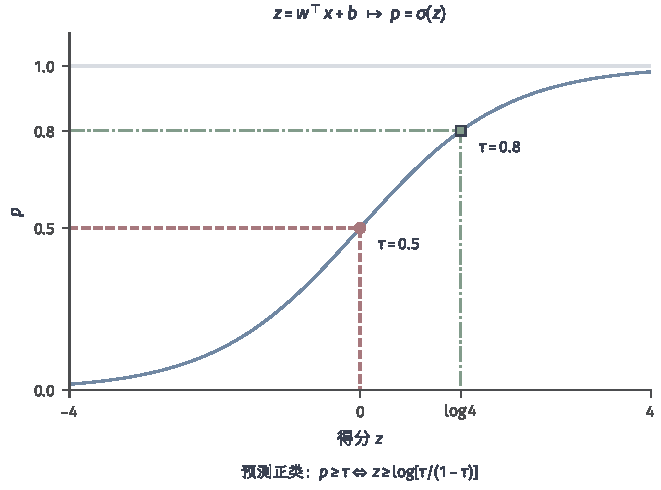
\includegraphics[width=105.412mm]{figures/03-models/01-classic-models/matplotlib/classification-logistic-probability/figure.pdf}
  \caption{线性得分$z=\bm{w}^{\top}\bm{x}+b$经Logistic函数转为正类概率$p$。蓝色实线为$p=\sigma(z)$；红色虚线与圆点标出$(0,0.5)$，绿色点划线与方点标出$(\log4,0.8)$。两组辅助线分别连接概率阈值与对应的得分阈值，数值是教学构造，不表示训练或校准结果。}
  \label{fig:classification-logistic-probability}
\end{figure}

\subsubsection{参数学习}
\label{sec:classification-logistic-learning}

对独立样本，模型给出的标签概率为$p_i^{y_i}(1-p_i)^{1-y_i}$，其中$p_i=\sigma(\bm{w}^{\top}\bm{x}_i+b)$。\term{最大似然估计}（maximum likelihood estimation, MLE）选择使已观察标签最可能出现的参数。其条件对数似然为
\begin{equation}
  \label{eq:classification-logistic-likelihood}
  \ell(\bm{w},b)
  =\sum_{i=1}^{n}
  \bigl[y_i\log p_i+(1-y_i)\log(1-p_i)\bigr].
\end{equation}
最大化$\ell$等价于最小化负对数似然$L=-\ell$，也就是二分类\term{交叉熵损失}（cross-entropy loss）：给真实标签分配的概率越低，惩罚越大。令增广输入$\tilde{\bm{x}}_i=(\bm{x}_i^{\top},1)^{\top}$、参数$\bm{\beta}=(\bm{w}^{\top},b)^{\top}\in\mathbb{R}^{d+1}$，并记$z_i=\tilde{\bm{x}}_i^{\top}\bm{\beta}$，可写成
\begin{equation}
  \label{eq:classification-logistic-loss}
  L(\bm{\beta})
  =\sum_{i=1}^{n}\bigl[\log(1+e^{z_i})-y_i z_i\bigr].
\end{equation}
数值计算不宜先求极端概率再取对数，可用$\log(1+e^z)=\max\{0,z\}+\log(1+e^{-|z|})$避免指数溢出。

为确定更新方向，利用$\sigma'(z)=\sigma(z)[1-\sigma(z)]$求导。令$\tilde{\bm{X}}\in\mathbb{R}^{n\times(d+1)}$的第$i$行为$\tilde{\bm{x}}_i^{\top}$，$\bm{p}=(p_1,\ldots,p_n)^{\top}$、$\bm{y}=(y_1,\ldots,y_n)^{\top}$，则
\begin{equation}
  \label{eq:classification-logistic-derivatives}
  \begin{aligned}
    \nabla L(\bm{\beta})
      &=\tilde{\bm{X}}^{\top}(\bm{p}-\bm{y}),\\
    \nabla^2 L(\bm{\beta})
      &=\tilde{\bm{X}}^{\top}\bm{R}\tilde{\bm{X}},\\
    \bm{R}
      &=\operatorname{diag}\bigl(p_i(1-p_i)\bigr)_{i=1}^{n}.
  \end{aligned}
\end{equation}
梯度中的$p_i-y_i$是预测概率与观察标签的差。对任意$\bm{v}\in\mathbb{R}^{d+1}$，Hessian的二次型为
\[
  \bm{v}^{\top}\nabla^2L\,\bm{v}
  =\sum_{i=1}^{n}p_i(1-p_i)
    (\tilde{\bm{x}}_i^{\top}\bm{v})^2\geq0.
\]
所以负对数似然$L$是凸函数，而被最大化的$\ell$是凹函数。有限参数处的$p_i(1-p_i)>0$；若$\tilde{\bm{X}}$列满秩，$L$严格凸，否则可能存在不改变训练得分的平坦方向。这涉及\term{可识别性}（identifiability）：数据能否区分不同参数。即使严格凸，也只能保证有限极小点若存在便唯一，不能保证它一定存在。

例如，若存在$\bm{\beta}_0$使$(2y_i-1)\tilde{\bm{x}}_i^{\top}\bm{\beta}_0>0$对所有样本成立，沿$t\bm{\beta}_0$令$t\to\infty$，每项损失均趋于零，但任意有限$t$的损失仍大于零。完全分离的数据因此没有有限MLE；准完全分离也可能使部分参数发散。完整的存在性分析需要区分分离、准分离和重叠情形\scite{albert1984existence}。

实际训练常加入$\lambda\lVert\bm{w}\rVert_2^2/2$，其中$\lambda>0$。这个$L_2$惩罚抑制权重无限增大，也改善病态方向的数值条件。若两类均有样本，所有权重都受惩罚而偏置不受惩罚，所得二分类目标仍有唯一有限极小点；但若训练集只有一类，偏置仍可独自趋于无穷。若连偏置也作正的二次惩罚，则整个增广参数方向都受约束。使用$\lambda\lVert\bm{w}\rVert_1$可得到稀疏权重，但目标不再处处可微，需要适合非光滑目标的求解步骤。

求解器的选择取决于数据规模和存储成本。稠密数据的一轮完整梯度计算为$O(nd)$，构造Hessian约为$O(nd^2)$，直接分解又需要$O(d^3)$。若存储$d\times d$量级的Hessian过于昂贵，\term{有限内存拟牛顿法}（limited-memory BFGS, L-BFGS）只保留少量历史更新来近似二阶信息。大规模稀疏数据则可采用\term{随机梯度下降}（stochastic gradient descent, SGD），每次用一个样本或小批量近似完整梯度。样本数、稀疏程度和精度要求共同决定求解选择。

数据持续到达时，也可以增量更新模型。McMahan等人的点击率系统使用稀疏正则与在线优化，展示了Logistic回归在大规模预测中的工程用途\scite{mcmahan2013}。增量训练省去了每次从头拟合的成本，但持续更新能否改善未来预测，仍取决于更新规则和数据变化。

对于中小规模问题，\term{迭代重加权最小二乘}（iteratively reweighted least squares, IRLS）把牛顿步改写为一个权重随当前预测变化的最小二乘问题。令$\bm{J}=\operatorname{diag}(1,\ldots,1,0)$，使偏置不受惩罚。在第$t$步计算
\begin{equation}
  \label{eq:classification-logistic-irls}
  \begin{aligned}
    u_i^{(t)}
      &=z_i^{(t)}
        +\frac{y_i-p_i^{(t)}}{p_i^{(t)}(1-p_i^{(t)})},\\
    \bm{\beta}^{(t+1)}
      &\in\argmin_{\bm{\beta}}\left\{
        \begin{aligned}
          &\frac12\sum_{i=1}^{n}\bm{R}_{i,i}^{(t)}
            (u_i^{(t)}-\tilde{\bm{x}}_i^{\top}\bm{\beta})^2\\
          &\quad{}+\frac{\lambda}{2}
            \bm{\beta}^{\top}\bm{J}\bm{\beta}
        \end{aligned}
      \right\}.
  \end{aligned}
\end{equation}
这里的$u_i^{(t)}$是供当前二次近似使用的工作响应，不是新标签。对应正规方程为
\[
  \bigl(\tilde{\bm{X}}^{\top}\bm{R}^{(t)}\tilde{\bm{X}}
       +\lambda\bm{J}\bigr)\bm{\beta}^{(t+1)}
  =\tilde{\bm{X}}^{\top}\bm{R}^{(t)}\bm{u}^{(t)}.
\]
将$\bm{u}^{(t)}$代入即可还原“当前参数减去Hessian逆作用于梯度”的牛顿步。实现时应解线性方程而不显式求逆，并用阻尼或线搜索控制更新；当$p_i$接近零或一时，直接计算工作响应可能不稳定，可改用梯度与Hessian求牛顿方向。停止条件可综合梯度范数、目标变化与最大迭代次数，牛顿法的局部快速收敛不意味着从任意初始化都可无阻尼运行\scite{hastie2009}。

\subsubsection{支持多分类（Softmax）}
\label{sec:classification-logistic-softmax}

新闻主题等任务需要在$C$个互斥类别中比较概率。\term{Softmax回归}（softmax regression，也称multinomial logistic regression）同时建立各类得分，并通过共同分母得到和为一的概率向量。其表示约束是任意两类的对数概率比为线性函数。

\textbf{模型结构。}为每类引入$\bm{w}_c\in\mathbb{R}^{d}$和$b_c\in\mathbb{R}$，令$z_c(\bm{x})=\bm{w}_c^{\top}\bm{x}+b_c$。其后验模型为
\begin{equation}
  \label{eq:classification-softmax-model}
  p_c(\bm{x})
  =\mathbb{P}(y=c\mid\bm{x})
  =\frac{\exp z_c(\bm{x})}
         {\sum_{r=1}^{C}\exp z_r(\bm{x})}.
\end{equation}
指数保证概率为正，分母保证归一化；两类之间的分母相消，得到
\[
  \log\frac{p_c(\bm{x})}{p_r(\bm{x})}
  =(\bm{w}_c-\bm{w}_r)^{\top}\bm{x}+b_c-b_r.
\]
当$C=2$时，$p_1(\bm{x})=\sigma((\bm{w}_1-\bm{w}_2)^{\top}\bm{x}+b_1-b_2)$。把第1类视为正类、第2类视为负类，就回到二分类Logistic回归。

共同增加得分不会改变概率。更具体地，对任意$\bm{a}\in\mathbb{R}^{d}$和$t\in\mathbb{R}$，变换$\bm{w}_c\mapsto\bm{w}_c+\bm{a}$、$b_c\mapsto b_c+t$使每个指数项同乘$\exp(\bm{a}^{\top}\bm{x}+t)$，因而全部约掉。这是$d+1$维的参数冗余。选择第$C$类为\term{参考类}（reference class），就是把该类完整的增广参数固定为零：
\begin{equation}
  \label{eq:classification-softmax-reference}
  \begin{gathered}
    \bm{w}_C=\bm{0},\qquad b_C=0,\\
    \log\frac{p_c(\bm{x})}{p_C(\bm{x})}
    =\bm{w}_c^{\top}\bm{x}+b_c
    \quad(c<C).
  \end{gathered}
\end{equation}
参考类约束需同时固定权重与偏置。$\lambda\sum_c\lVert\bm{w}_c\rVert_2^2/2$只消除共同权重平移，还须例如令$\sum_c b_c=0$或惩罚全部偏置，才能锁定共同偏置平移。参数冗余消除后，设计矩阵的秩决定数据能否区分剩余方向，数据分离则影响有限解的存在性。

\textbf{参数学习。}现在$y_i\in\{1,\ldots,C\}$，记$p_{i,c}=p_c(\bm{x}_i)$，$\bm{\Theta}\in\mathbb{R}^{(d+1)\times C}$的第$c$列为$\bm{\beta}_c=(\bm{w}_c^{\top},b_c)^{\top}$。多类负对数似然是
\begin{equation}
  \label{eq:classification-softmax-loss}
  \begin{aligned}
    L(\bm{\Theta})
      &=-\sum_{i=1}^{n}\log p_{i,y_i}\\
      &=\sum_{i=1}^{n}\left[
        \log\sum_{c=1}^{C}e^{z_c(\bm{x}_i)}
        -z_{y_i}(\bm{x}_i)\right].
  \end{aligned}
\end{equation}
以$\mathbb{1}\{\cdot\}$表示条件成立时为一、否则为零的指示函数，梯度为
\begin{equation}
  \label{eq:classification-softmax-gradient}
  \begin{aligned}
    \nabla_{\bm{w}_c}L
      &=\sum_{i=1}^{n}
        [p_{i,c}-\mathbb{1}\{y_i=c\}]\bm{x}_i,\\
    \frac{\partial L}{\partial b_c}
      &=\sum_{i=1}^{n}
        [p_{i,c}-\mathbb{1}\{y_i=c\}].
  \end{aligned}
\end{equation}
它仍由“预测减观察”的残差驱动。Hessian的$(c,r)$参数块为
\[
  \nabla^2_{\bm{\beta}_c,\bm{\beta}_r}L
  =\sum_{i=1}^{n}p_{i,c}
    [\mathbb{1}\{c=r\}-p_{i,r}]
    \tilde{\bm{x}}_i\tilde{\bm{x}}_i^{\top}.
\]
对任意增广参数扰动$\bm{v}_c$，令$a_{i,c}=\tilde{\bm{x}}_i^{\top}\bm{v}_c$，相应二次型为
\[
  \sum_{i=1}^{n}\left[
    \sum_{c=1}^{C}p_{i,c}a_{i,c}^2
    -\left(\sum_{c=1}^{C}p_{i,c}a_{i,c}\right)^2
  \right]\geq0.
\]
方括号正是以$\bm{p}_i$为权重的方差，故$L$凸。共同平移使方差为零，秩亏还会引入其他平坦方向；分离数据上同样可能不存在有限MLE。参考类约束解决表示冗余，适当正则化控制参数大小，两者的作用不同。

Softmax可用分块牛顿法、L-BFGS或小批量SGD优化，多类Hessian还包含类别间的耦合，不能简单把$C$个独立的二分类IRLS问题拼起来。求概率时应先减去$m(\bm{x})=\max_c z_c(\bm{x})$，用$e^{z_c-m}/\sum_r e^{z_r-m}$得到完全相同且更稳定的结果。普通稠密实现的一轮梯度计算约为$O(ndC)$。

类别特别多时，分母求和也会成为瓶颈。\term{层次Softmax}（hierarchical softmax）以树上路径概率的乘积替代平坦分类参数化；\term{噪声对比估计}（noise-contrastive estimation, NCE）通过区分数据与人为噪声来估计模型；\term{负采样}（negative sampling）只对抽取的负例建立局部区分目标。三种方法通过不同参数化或估计目标减少计算，其中负采样通常改变原Softmax训练目标\scite{goodfellow2016}。

\textbf{决策与概率语义。}预测可取$\hat y(\bm{x})=\argmax_c p_c(\bm{x})=\argmax_c z_c(\bm{x})$，并按固定类别次序处理平局。Softmax输出已经满足概率公理，却不自动满足\term{概率校准}（probability calibration）：在被预测为某类概率约为$0.8$的样本中，该类的实际比例也应接近$0.8$。有限样本、模型失配、正则化和分布变化都可能破坏这种对应。

Softmax也可用作神经网络的分类输出层。归一化给出合法概率向量，置信度是否对应实际正确频率还需检验。Guo等在现代网络中观察到准确率与校准质量的差异，并在一些实验设置下用独立验证数据的温度缩放改善校准\scite{guo2017calibration}。

\subsubsection{小结}
\label{sec:classification-logistic-summary}

Logistic回归以线性得分表示条件概率，再由阈值联系到误判代价；Softmax将这一机制扩展为多类联合比较。固定特征表示下的目标凸，权重可在对数几率尺度解释。参数约束决定可识别性，分离状况影响有限解存在性，样本外频率检验概率质量，三者需各自确定。

它的表示限制来自线性对数几率：若需要非线性交互，应显式加入交叉项或其他特征变换。训练可通过随机优化增量进行，预测则只需保存参数并计算得分。信用评分、医学风险预测和点击率预估都可以采用这种基线，但具体特征与验证方式需要对应到各自任务。

\subsection{朴素贝叶斯}
\label{sec:classification-naive-bayes}

若希望通过“哪一类更可能产生当前输入”来分类，就需要估计类条件分布。困难在于，$d$个二值特征已有$2^d$种组合，逐一统计需要大量样本。\term{朴素贝叶斯}（naive Bayes, NB）把复杂的联合分布拆成较小的分布，用简化假设换取少量统计量和直接的参数估计。这样的约束可能降低有限样本下的估计波动，也可能引入持续的模型偏差，并不无条件提高精度。

Maron在1961年关于自动索引的研究，是概率方法用于文档归类的早期工作之一。文档分类需要从大量词项中提取可累积的类别证据，这也成为朴素贝叶斯的一项典型用途\scite{maron1961indexing}。

\subsubsection{模型结构}
\label{sec:classification-naive-bayes-structure}

对一般特征向量，NB采用给定类别后的\term{条件独立}（conditional independence）假设：已知$y=c$后，一个特征的取值不再改变其他特征的分布。令$\pi_c=\mathbb{P}(y=c)$、$p_{j,c}(x_j)=p(x_j\mid y=c)$，模型写成
\begin{equation}
  \label{eq:classification-naive-bayes-model}
  \begin{aligned}
    q_c(\bm{x})&=\prod_{j=1}^{d}p_{j,c}(x_j),\\
    \mathbb{P}_{\mathrm{NB}}(y=c\mid\bm{x})
      &=\frac{\pi_c q_c(\bm{x})}
      {\sum_{r=1}^{C}\pi_r q_r(\bm{x})}.
  \end{aligned}
\end{equation}
记号$q_c$强调这是模型使用的乘积分布，未必等于真实类条件分布。条件独立不要求全部训练样本混在一起时特征仍独立，例如词项之间的总体相关性可能部分来自主题差异。

只需要分类时，各类共同的分母可以省略。为避免许多小概率连乘下溢，通常比较对数得分
\begin{equation}
  \label{eq:classification-naive-bayes-score}
  s_c(\bm{x})
  =\log\pi_c+\sum_{j=1}^{d}\log p_{j,c}(x_j),
  \qquad
  \hat y(\bm{x})=\argmax_c s_c(\bm{x}).
\end{equation}
这里$s_c$不是归一化的对数后验；需要概率时还须减去$\log\sum_r e^{s_r}$。零概率可使得分为负无穷，后面的平滑正是为未见事件保留概率质量。文档的多项式版本沿用相似得分，但它的独立性对象是词元位置，而非总长度固定后的各维计数，必须另外说明。

\subsubsection{参数学习}
\label{sec:classification-naive-bayes-learning}

令$n_c=\sum_i\mathbb{1}\{y_i=c\}$，类先验的MLE为$\hat\pi_c=n_c/n$。这是以训练样本的类别比例估计目标总体的比例，依赖抽样具有代表性；人为重采样改变类别比例，部署先验需要按抽样机制修正或另行估计。也可以使用有依据的外部类别比例；若希望保留对该比例的不确定性，并为训练中未见的类别保留概率质量，则可对类概率向量$\bm{\pi}=(\pi_1,\ldots,\pi_C)^{\top}$设置参数先验。以下对类别概率与各组类条件参数设置相互独立的先验，以便分别更新。

给类概率向量设置正参数$\gamma_c$的\term{Dirichlet分布}先验（分布形式参考\BookSectionRef{sec:probability-common-distributions}{第一卷“数学准备”的“随机变量的分布模型表示”小节}）。
独立类别记录的计数进入各坐标的幂次，因而
\[
  \begin{aligned}
    p(\bm{\pi})
      &\propto\prod_{c=1}^{C}\pi_c^{\gamma_c-1},\\
    p(y_1,\ldots,y_n\mid\bm{\pi})
      &\propto\prod_{c=1}^{C}\pi_c^{n_c},\\
    p(\bm{\pi}\mid y_1,\ldots,y_n)
      &\propto\prod_{c=1}^{C}\pi_c^{\gamma_c+n_c-1}.
  \end{aligned}
\]
后验仍是Dirichlet分布，只需把参数从$\gamma_c$更新为$\gamma_c+n_c$。
这种先验与后验属于同一分布族的关系称为\term{共轭}（conjugacy）。
由Dirichlet分布的均值公式，后验均值为
\[
  \tilde\pi_c=\frac{n_c+\gamma_c}
  {n+\sum_{r=1}^{C}\gamma_r}.
\]
先验均值为$\gamma_c/\sum_r\gamma_r$，参数总和决定这些伪计数相对于观测计数的权重。这里“类别先验$\pi_c$”是样本生成模型的一部分，“参数先验”则表达估计$\bm{\pi}$前的不确定性，两者分别属于样本生成层与参数估计层。

连续特征可采用\term{高斯朴素贝叶斯}（Gaussian naive Bayes），即$x_j\mid y=c\sim\mathcal{N}(\mu_{j,c},\sigma_{j,c}^{2})$，其中$\sigma_{j,c}^{2}>0$。当$n_c>0$且该特征的类内平方偏差和为正时，均值和方差的MLE为
\begin{equation}
  \label{eq:classification-naive-bayes-gaussian}
  \begin{aligned}
    \hat\mu_{j,c}
      &=\frac{1}{n_c}\sum_{i:y_i=c}x_{i,j},\\
    \hat\sigma_{j,c}^{2}
      &=\frac{1}{n_c}\sum_{i:y_i=c}
        (x_{i,j}-\hat\mu_{j,c})^2.
  \end{aligned}
\end{equation}
方差分母为$n_c$，不是无偏样本方差所用的$n_c-1$。在上述条件下，预测时将这些量代入一维高斯密度后相乘。若某类某特征恒定为$a$，固定$\mu_{j,c}=a$后，对数似然为$-n_c\log(2\pi\sigma_{j,c}^{2})/2$，随正方差趋于零而无界增大。因此，此时正方差参数域内没有有限MLE；式\eqref{eq:classification-naive-bayes-gaussian}给出的零值只是样本散度，不能代入普通高斯密度。设定有明确尺度的方差下限或加入先验后，得到的是相应的受约束或正则化估计；给密度任意“加一”不是离散概率的平滑对应物。

只关心某个词是否出现时，可用\term{伯努利朴素贝叶斯}（Bernoulli naive Bayes）。输入$x_{i,j}\in\{0,1\}$，令$n_{j,c}=\sum_{i:y_i=c}x_{i,j}$，则
\begin{equation}
  \label{eq:classification-naive-bayes-bernoulli}
  \begin{aligned}
    q_c(\bm{x})
      &=\prod_{j=1}^{d}
        \theta_{j,c}^{x_j}(1-\theta_{j,c})^{1-x_j},\\
    \hat\theta_{j,c}&=\frac{n_{j,c}}{n_c}.
  \end{aligned}
\end{equation}
$x_j=0$也通过词缺失概率提供证据，因此两种取值的项都参与得分；这里的MLE要求$n_c>0$。
为平滑这个二值事件，使用Beta分布作为$\theta_{j,c}$的先验，
两个正参数$\alpha_1,\alpha_0$分别对应出现与未出现。乘以似然后，
两项指数分别增加$n_{j,c}$和$n_c-n_{j,c}$，所以
\[
  \theta_{j,c}\mid D_n
  \sim\operatorname{Beta}
    (\alpha_1+n_{j,c},\,\alpha_0+n_c-n_{j,c}).
\]
其后验均值为$(n_{j,c}+\alpha_1)/(n_c+\alpha_1+\alpha_0)$；对称情形$\alpha_1=\alpha_0=\alpha$的分母是$n_c+2\alpha$。这同时平滑了出现和未出现两种事件。

若重复出现的次数也有意义，应使用\term{多项式朴素贝叶斯}（multinomial naive Bayes）。设固定词表有$d$个词项，$\bm{x}_i\in\mathbb{N}_0^d$记录一篇文档的词项计数，$m_i=\sum_jx_{i,j}$是该文档的总词元数。给定类别和$m_i$，假设每个词元位置独立地按$\bm{\theta}_c=(\theta_{1,c},\ldots,\theta_{d,c})^{\top}$抽取词项，其中$\sum_j\theta_{j,c}=1$。忽略顺序后，计数向量服从
\begin{equation}
  \label{eq:classification-naive-bayes-multinomial}
  \mathbb{P}(\bm{x}_i\mid y_i=c,m_i)
  =\frac{m_i!}{\prod_{j=1}^{d}x_{i,j}!}
    \prod_{j=1}^{d}\theta_{j,c}^{x_{i,j}}.
\end{equation}
因为计数总和已固定，各维计数并不独立。将它写成每维整数取值的独立类别分布，会改变模型和分母。McCallum与Nigam专门比较了伯努利和多项式这两种文档事件模型，明确区分“词是否出现”与“词出现多少次”\scite{mccallum1998event}。

标准文档分类通常进一步假设长度分布与类别无关，因而$\mathbb{P}(m_i\mid y_i=c)$在类别比较中约掉，此时给定长度后的类先验仍为$\pi_c$。若长度本身携带类别信息，则应保留并估计该项，使长度也参与后验计算。

令$t_{j,c}=\sum_{i:y_i=c}x_{i,j}$为第$c$类中词项$j$的总出现次数，$t_c=\sum_jt_{j,c}$为该类的总词元数。去掉与参数无关的组合系数后，类内对数似然为$\sum_jt_{j,c}\log\theta_{j,c}$。当$t_c>0$时，在$\sum_j\theta_{j,c}=1$约束下求极值，正计数坐标上的拉格朗日方程给出$t_{j,c}/\theta_{j,c}$为同一常数，零计数坐标取零；求和确定常数为$t_c$，从而得到频率MLE。

若对$\bm{\theta}_c$使用$\operatorname{Dirichlet}(\alpha_1,\ldots,\alpha_d)$先验，其中$\alpha_j>0$，同样的共轭更新把各坐标的幂次从$\alpha_j-1$变为$\alpha_j+t_{j,c}-1$，得到
\[
  \bm{\theta}_c\mid D_n
  \sim\operatorname{Dirichlet}
    (\alpha_1+t_{1,c},\ldots,\alpha_d+t_{d,c}).
\]
把更新后的参数归一化即可得到后验均值。两种估计分别为
\begin{equation}
  \label{eq:classification-naive-bayes-smoothing}
  \hat\theta_{j,c}=\frac{t_{j,c}}{t_c},
  \qquad
  \tilde\theta_{j,c}
  =\frac{t_{j,c}+\alpha_j}
         {t_c+\sum_{r=1}^{d}\alpha_r}.
\end{equation}
前式要求$t_c>0$；后式也给出下一词元的后验预测概率，因为给定参数时该概率为$\theta_{j,c}$，对参数后验积分便得到其后验均值。这种均值估计通常既不同于MLE，也不同于式\eqref{eq:regression-map}定义的MAP。对称$\alpha_j=1$给出\term{拉普拉斯平滑}（Laplace smoothing），相当于每个词项加入一个伪计数；$\alpha_j=1/2$对应多项式参数的Jeffreys先验。对伯努利参数，其对应物是$\operatorname{Beta}(1/2,1/2)$，不应把这些常数不加区分地推广到高斯方差。以平滑估计代入式\eqref{eq:classification-naive-bayes-multinomial}得到的是常用的点估计分类器，不等于积分消去参数后的整篇文档预测分布。

在长度与类别无关的约定下，文档预测只需计算$\log\tilde\pi_c+\sum_jx_j\log\tilde\theta_{j,c}$。算法\ref{alg:classification-multinomial-nb}给出完整的统计与预测流程，训练和预测使用相同的词表，并明确处理平滑与得分平局。
\begin{algorithm}[带平滑的多项式朴素贝叶斯]
  \label{alg:classification-multinomial-nb}
  \begin{algorithmic}[1]
    \Require 非空训练集$D_n$，固定词表大小$d$与类别数$C$；
    \Statex \hspace{\algorithmicindent} 词项伪计数$\alpha>0$，类别伪计数$\gamma>0$
    \Ensure 类先验$\tilde{\bm{\pi}}$、词项概率$\tilde{\bm{\Theta}}$及预测规则
    \State 检查所有输入为有限非负整数计数，标签属于$\{1,\ldots,C\}$
    \State 将$n_c$、$t_c$与$t_{j,c}$全部初始化为零
    \For{$i=1,\ldots,n$}
      \State 令$c=y_i$，并更新$n_c\gets n_c+1$
      \For{满足$x_{i,j}>0$的词项$j$}
        \State $t_{j,c}\gets t_{j,c}+x_{i,j}$
        \State $t_c\gets t_c+x_{i,j}$
      \EndFor
    \EndFor
    \For{$c=1,\ldots,C$}
      \State $\tilde\pi_c\gets(n_c+\gamma)/(n+C\gamma)$
      \State 对所有$j$，令$\tilde\theta_{j,c}\gets(t_{j,c}+\alpha)/(t_c+d\alpha)$
    \EndFor
    \State 对新计数向量$\bm{x}$，按相同词表与输入检查计算
    \Statex \hspace{\algorithmicindent}
      $s_c=\log\tilde\pi_c+\sum_{j:x_j>0}x_j\log\tilde\theta_{j,c}$
    \State 返回$s_c$最大的类别；平局时返回索引最小的类别
  \end{algorithmic}
\end{algorithm}

假设词表只有三个词项，两类累计计数分别为$(3,1,0)$和$(0,1,3)$，类先验均为$1/2$。取$\alpha=1$，平滑后的词项概率分别为$(4,2,1)/7$和$(1,2,4)/7$。对新文档$\bm{x}=(1,0,1)^{\top}$，两类乘积相同，判决平局；对$\bm{x}=(2,0,1)^{\top}$，两类得分之差为$\log4$，于是选择第1类。这个教学例子显示了重复计数怎样改变证据，而零计数词项经平滑后不会把整类概率直接清零。

\subsubsection{理论分析}
\label{sec:classification-naive-bayes-theory}

\paragraph{表达能力}
朴素贝叶斯用类条件乘积分布表示类别，借此压缩高维联合概率表。代价是省略给定类别后的特征相互作用；类别排序与完整联合密度的拟合是不同目标，前者正确时后者仍可能有偏差。

\paragraph{收敛性}
对有限离散特征，经验频率直接达到相应多项式似然的最大值，允许概率取零；各组条件概率可分别求解。加入正伪计数后直接计算的是后验均值，其估计目标包含参数先验。高斯NB在各组有样本且样本方差为正时取得有限MLE；退化组需另加方差约束或先验。训练只需累积统计量，稠密输入约需$O(nd)$运算，没有迭代收敛速度的问题。

\paragraph{泛化性}
闭式估计是否足以支持新样本预测，要先检查样本增加后这些估计量趋向什么。固定特征维数、类别数和有限取值集合，在独立同分布抽样且各类先验为正时，强大数定律保证经验类频率和类内相对频率几乎必然收敛到对应的真实概率。固定伪计数相对于不断增长的类内样本数趋于零，因此不改变这一极限。

单维条件概率的频率一致性来自样本抽样和大数定律；将它们相乘以还原联合分布，还需要类条件独立假设。高斯NB的密度一致性要求高斯族正确、方差非退化及一致估计。多项式NB需正确指定词元生成与长度处理，并使文档抽样和总计数满足相应大数定律。下面在有限离散情形同时证明频率与风险收敛。

估计量收敛后，还需回答由这些估计构造的分类器能否接近贝叶斯风险。下面先在模型正确的有限离散情形下给出完整证明，再考察条件独立不成立时，哪些依赖会改变决策。结论描述样本数趋于无穷时的风险，且允许后验平局。
\begin{theorem}[有限离散特征下NB的风险一致性]
  \label{thm:classification-naive-bayes-consistency}
  设$d$、$C$固定，每维特征的取值集合有限，训练样本独立同分布，且每类先验$\pi_c>0$。若真实分布满足给定类别后的特征条件独立，使用经验类频率与类内相对频率估计概率，或加入固定的正伪计数，则所得NB分类器$\hat h_n$满足
  \[
    R(\hat h_n)\longrightarrow R^\ast
    \quad\text{几乎必然}.
  \]
  这里$R(h)=\mathbb{P}(h(\bm{X})\neq Y)$针对独立的新样本计算，$R^\ast$为贝叶斯风险；几乎必然收敛针对无限训练样本序列。早期若$n_c=0$，可任意指定该类的条件分布；若某输入的全部类别得分为零，也可任意指定该处的预测。
\end{theorem}
\begin{proof}
  对取值$v$及$n_c>0$的类别，类内估计为
  \[
    \hat p_{j,c}(v)
    =\frac{\sum_{i=1}^{n}\mathbb{1}\{x_{i,j}=v,y_i=c\}}
           {n_c}.
  \]
  由强大数定律，$n_c/n\to\pi_c>0$，故空类别事件几乎必然最终不再出现。分子除以$n$收敛到$\mathbb{P}(X_j=v,Y=c)$，因此$\hat p_{j,c}(v)\to p_{j,c}(v)$几乎必然。固定伪计数相对于$n_c$趋于零，不改变极限。有限多个估计可同时收敛；对每个$\mathbb{P}(\bm{X}=\bm{x})>0$的输入，归一化分母最终为正，早期任意约定不影响极限。乘积与归一化于是给出
  \[
    \hat\eta_{n,c}(\bm{x})
    \longrightarrow
    \eta_c(\bm{x})=\mathbb{P}(Y=c\mid\bm{X}=\bm{x}).
  \]
  令$c^\ast$最大化真实后验，$\hat c$最大化估计后验。因为$\hat\eta_{n,\hat c}\geq\hat\eta_{n,c^\ast}$，插入这两个估计值得到
  \[
    0\leq\eta_{c^\ast}(\bm{x})-\eta_{\hat c}(\bm{x})
    \leq2\max_c|\hat\eta_{n,c}(\bm{x})-\eta_c(\bm{x})|.
  \]
  左侧就是该输入处的超额分类风险。对有限个输入按真实概率加权求和，右侧趋于零，故整体风险趋于$R^\ast$。
\end{proof}

后验平局时，最大化类别可随$n$改变，而每个最优类别具有相同风险。因此风险一致性允许标签选择继续变化。模型失配时，频率估计可能趋于稳定的乘积分布，但该分布不同于真实联合分布；增加样本减小的是估计误差，模型偏差仍需改变表示才能处理。

真实数据中的词语、测量量和相邻像素常有依赖，但违反独立性并不直接决定分类误差。Domingos与Pazzani在1997年的研究区分了概率估计误差与零一分类损失，报告了含依赖数据上的经验结果，并在特定条件下分析了合取、析取概念等情形的最优性。分类只要求最高得分类别正确，因此概率估计失真与分类仍然准确可以同时发生\scite{domingos1997optimality}。

为拆开这些层次，暂取二分类$c\in\{0,1\}$，并使用真实类先验与真实单维条件分布构造总体NB，不含有限样本估计误差。在下列分母均为正的输入处，定义
\begin{equation}
  \label{eq:classification-naive-bayes-ratios}
  \begin{aligned}
    r(\bm{x})
      &=\frac{\pi_1p(\bm{x}\mid y=1)}
              {\pi_0p(\bm{x}\mid y=0)},\\
    r_{\mathrm{NB}}(\bm{x})
      &=\frac{\pi_1\prod_jp(x_j\mid y=1)}
              {\pi_0\prod_jp(x_j\mid y=0)}.
  \end{aligned}
\end{equation}
若平局都归第1类，则两个分类器在该输入上的决策相同，当且仅当$r\geq1$与$r_{\mathrm{NB}}\geq1$同真同假。理由只是：用正的第0类联合得分除两边，不改变类别得分的大小关系。这个等价关系揭示正确决策依赖两组得分的相对大小；其中$r$仍包含未知真分布。

要解释依赖何时不会改变比值，可以进一步定义
\begin{equation}
  \label{eq:classification-naive-bayes-dependence}
  \begin{aligned}
    a_c(\bm{x})
      &=\frac{p(\bm{x}\mid y=c)}
              {\prod_{j=1}^{d}p(x_j\mid y=c)},\\
    r(\bm{x})
      &=r_{\mathrm{NB}}(\bm{x})
        \frac{a_1(\bm{x})}{a_0(\bm{x})}.
  \end{aligned}
\end{equation}
$a_c$衡量真实联合分布相对于乘积分布的修正。条件独立使$a_c=1$；更弱的充分条件是$a_1=a_0>0$，此时即使两类内部都有依赖，其修正在类别比值中也完全相消。由概率链式法则还可写成
\[
  a_c(\bm{x})
  =\prod_{j=1}^{d}
    \frac{p(x_j\mid x_1,\ldots,x_{j-1},y=c)}
         {p(x_j\mid y=c)}.
\]
各因子不必分别为一，不同位置的修正也可在整体乘积中抵消。所需比较的是两类中这些概率修正的比值，而不只是通常的相关系数。Zhang在2004年以局部依赖比和全局依赖分布因子展开了这一思路\scite{zhang2004optimality}。

完全相消仍只是充分条件。若$r_{\mathrm{NB}}\neq1$，且
\[
  \left|\log a_1(\bm{x})-\log a_0(\bm{x})\right|
  <\left|\log r_{\mathrm{NB}}(\bm{x})\right|,
\]
则修正不足以改变对数比的正负，决策仍然相同。反之，依赖影响在两类中不均衡时就可能越过边界。例如把一个有信息的二值特征原样复制一次，在等类先验下，NB把原似然比平方：原比值为4时，真实后验为$4/5$，NB却报$16/17$，分类未变而置信度偏高。非等先验下，特征证据被重复计算还可能改变类别，这说明同一个依赖错误对概率与决策的影响可以不同。

\subsubsection{小结}
\label{sec:classification-naive-bayes-summary}

NB的计算优势来自统计量可累积：稠密输入的训练统计约为$O(nd)$，存储为$O(Cd)$，单样本预测为$O(Cd)$，这些量级以每维分布的参数个数有界为前提。以$\bm{X}\in\mathbb{R}^{n\times d}$记训练输入矩阵，多项式模型可按非零计数累积，训练约为$O(n+\operatorname{nnz}(\bm{X})+Cd)$，预测约为$O(C(1+\operatorname{nnz}(\bm{x})))$。这里$\operatorname{nnz}$表示非零元素数；“扫描一次”不意味着与样本数、特征数和类别数都无关。

它适合建立文档、垃圾邮件和情感分类的低成本基线，也容易增量更新。Graham在2002年8月的《A Plan for Spam》中介绍了基于词项统计的邮件过滤实践；该方法还加入词项筛选与经验修正，与本节的标准多项式模型有所不同\scite{graham2002spam}。

使用NB时要分别检查输入的事件模型、特征依赖和概率校准。相关性可能造成证据重复计算，却不必然破坏分类；连续特征还可能因所选单维分布失配而出错。若业务需要可靠概率，应另用留出数据评估和校准，而不只报告准确率。

\subsection{高斯判别分析（GDA）}
\label{sec:classification-gda}

高斯NB只保存每维的均值与方差，相当于把类内协方差矩阵的非对角元素设为零。若分类信息恰好体现在多个连续特征的共同变化中，就需要估计这些关系。\term{高斯判别分析}（Gaussian discriminant analysis, GDA）用每类的多元高斯分布描述输入，允许保留类内协方差；增加的表达能力也意味着需要估计更多参数。

第\ref{sec:clustering-gmm}节的高斯混合模型同样估计高斯成分及其权重，但成分归属是潜变量，通常用\term{期望最大化}（expectation-maximization, EM）交替计算成分归属的后验概率并更新分布参数；两步计算的分类实例见第\ref{sec:classification-semisupervised-comparison}节。GDA中的类别标签已经观测，可以直接按类分组估计。两者共享高斯密度结构，却分别服务于预设类别预测和无标签分组。

从类间分离程度转向概率决策，关注的问题也从“怎样区分类别”扩展为“怎样权衡误判”。Anderson在1951年的多元分类研究中，以误分类代价为依据讨论分类规则，并在正态总体下给出判别函数。这为理解GDA提供了一条历史线索：分布模型负责描述输入来自各类的可能性，决策规则再据此比较误判代价，而不只是寻找一个投影方向\scite{anderson1951classification}。

\subsubsection{模型结构}
\label{sec:classification-gda-structure}

本节用GDA统称各类具有高斯条件分布的判别模型，并分别讨论共享协方差与类特有协方差。对第$c$类，参数是$\pi_c$、$\bm{\mu}_c\in\mathbb{R}^{d}$及对称正定的$\bm{\Sigma}_c\in\mathbb{R}^{d\times d}$：
\begin{equation}
  \label{eq:classification-gda-density}
  \begin{aligned}
    p(\bm{x}\mid y=c)
      &=\frac{\exp[-\Delta_c(\bm{x})/2]}
        {(2\pi)^{d/2}|\bm{\Sigma}_c|^{1/2}},\\
    \Delta_c(\bm{x})
      &=(\bm{x}-\bm{\mu}_c)^{\top}
        \bm{\Sigma}_c^{-1}(\bm{x}-\bm{\mu}_c).
  \end{aligned}
\end{equation}
这里的二次型$\Delta_c$按类内变化尺度衡量输入偏离均值的程度；行列式项补偿分布体积，在不同协方差的类别比较中同样参与得分。贝叶斯后验仍为$\pi_cp(\bm{x}\mid y=c)/\sum_r\pi_rp(\bm{x}\mid y=r)$。

取对数并删除所有类别共有的$-d\log(2\pi)/2$，得到判别得分
\begin{equation}
  \label{eq:classification-gda-score}
  g_c(\bm{x})
  =\log\pi_c-\frac12\log|\bm{\Sigma}_c|
   -\frac12\Delta_c(\bm{x}).
\end{equation}
预测选择最大$g_c$。这一模型不要求各特征独立，但要求整类分布可由单个多元高斯刻画；完整协方差保留全部二阶关系，单个高斯成分仍限制了非线性依赖和多峰结构的表达。

\subsubsection{参数学习}
\label{sec:classification-gda-learning}

有标签时，各类样本的归属已知，联合对数似然可按类别分开优化。当每类都有样本且类内散度矩阵正定时，MLE为
\begin{equation}
  \label{eq:classification-gda-estimates}
  \begin{aligned}
    \hat\pi_c&=\frac{n_c}{n},\\
    \hat{\bm{\mu}}_c
      &=\frac{1}{n_c}\sum_{i:y_i=c}\bm{x}_i,\\
    \hat{\bm{\Sigma}}_c
      &=\frac{1}{n_c}\sum_{i:y_i=c}
        (\bm{x}_i-\hat{\bm{\mu}}_c)
        (\bm{x}_i-\hat{\bm{\mu}}_c)^{\top}.
  \end{aligned}
\end{equation}
均值来自使类内平方偏差最小的驻点，协方差来自似然中的对数行列式与二次型之间的平衡。和高斯NB一样，这里使用MLE分母$n_c$；若改用$n_c-1$，得到的是无偏协方差估计。若类内散度奇异，沿未被样本覆盖的方向收缩方差可使似然不断增大，在协方差正定的参数域内没有有限MLE；此时上式的奇异矩阵只能作为样本散度统计，不能当成合法的普通高斯协方差。

共享协方差特例的完整推导已经放在第\ref{sec:classification-lda}节。简要地说，约束$\bm{\Sigma}_c=\bm{\Sigma}$后，合并类内散度给出式~\eqref{eq:classification-lda-covariance}~的MLE；展开高斯得分时，各类共有的$\bm{x}^{\top}\bm{\Sigma}^{-1}\bm{x}$相消，得到式~\eqref{eq:classification-lda-score}~的线性得分。两类得分相等因而给出超平面。若协方差随类变化，二次项一般不能约掉，得到QDA及通常为二次曲面的两类边界。两者沿用贝叶斯规则，协方差约束改变允许的分布族和得分形式\scite{bishop2006}。

图\ref{fig:classification-gaussian-boundaries}在同一个二维教学例子中比较两种协方差设定。两图都取$\pi_1=\pi_2=1/2$、$\bm{\mu}_1=(-1,0)^{\top}$、$\bm{\mu}_2=(1,0)^{\top}$，坐标为无量纲特征。左图共享$\bm{\Sigma}_1=\bm{\Sigma}_2=\bm{I}_2$；右图只将第2类改为$\bm{\Sigma}_2=\operatorname{diag}(1,4)$。代入式\eqref{eq:classification-gda-score}，得分差分别为
\begin{equation}
  \label{eq:classification-gda-boundary-example}
  \begin{aligned}
    g_2-g_1&=2x_1
      &&\text{（共享协方差）},\\
    g_2-g_1&=2x_1+\frac38x_2^2-\log2
      &&\text{（类特有协方差）}.
  \end{aligned}
\end{equation}
令得分差为零，得到直线$x_1=0$和抛物线$x_1=\frac12\log2-\frac{3}{16}x_2^2$。在两种设定中，边界右侧的$g_2$都更大，预测第2类。右图中，第2类沿$x_2$方向更分散：在$x_2=0$附近，行列式项降低了它的密度峰值，边界向右移到$x_1\approx0.347$；随着$|x_2|$增大，第2类较慢衰减的密度又使其预测区域向左延伸。只看均值之间的距离，会漏掉方差尺度和密度归一化对判决的共同影响。
\begin{figure*}[htbp]
  \centering
  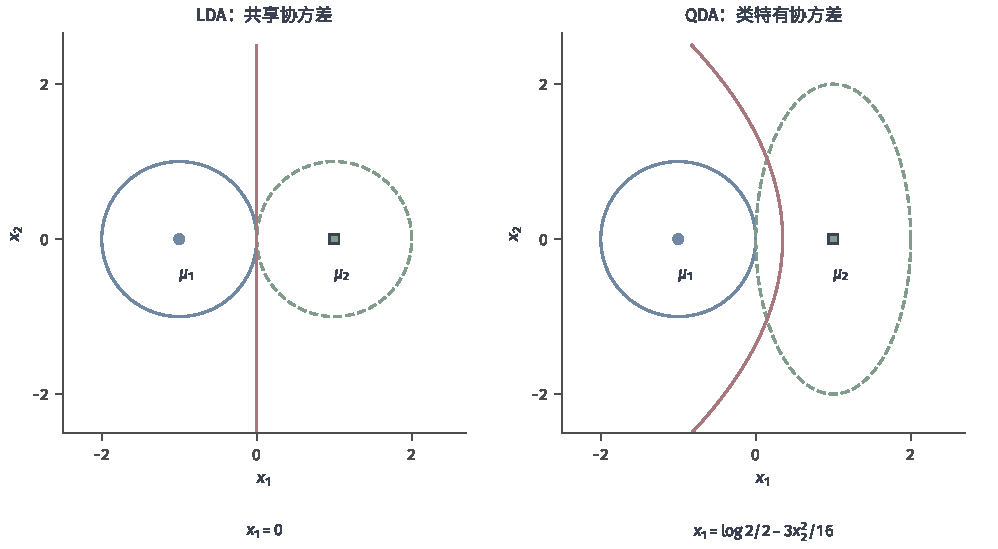
\includegraphics[width=159.059mm]{figures/03-models/01-classic-models/matplotlib/classification-gaussian-boundaries/figure.pdf}
  \caption{两图均取$\pi_1=\pi_2=1/2$、$\bm{\mu}_1=(-1,0)^{\top}$、$\bm{\mu}_2=(1,0)^{\top}$和$\bm{\Sigma}_1=\bm{I}_2$，仅第2类协方差变化。蓝色圆点和绿色方点为均值，蓝色实线与绿色虚线分别为$\Delta_1=1$和$\Delta_2=1$的等密度轮廓；不同类的这些轮廓不保证密度值相同。红色粗线按$g_1=g_2$的解析式绘制，底部公式分别给出LDA的线性边界与QDA的二次边界。参数均为教学构造，不是采样或拟合结果。}
  \label{fig:classification-gaussian-boundaries}
\end{figure*}

对二分类，把式~\eqref{eq:classification-lda-score}~中的两类得分相减并归一化，就得到Logistic形式的后验。因此，共享高斯假设蕴含线性对数几率，反过来却不成立；许多非高斯输入分布也能有Logistic形式的条件概率。即便两条路线的后验形式相同，用联合似然估计均值和协方差，与直接最大化条件似然，也通常得到不同的有限样本参数。

完整协方差每类需要$d(d+1)/2$个自由参数。类内散布矩阵的秩至多为$n_c-1$，因而$n_c\leq d$时必然奇异，不能直接代入普通高斯密度；$n_c>d$也不保证估计准确或条件良好。共享估计的秩至多为$n-C$。在维数较大或类别样本少时，可以共享、取对角，或采用
\[
  \tilde{\bm{\Sigma}}_c
  =(1-\rho)\hat{\bm{\Sigma}}_c+\rho\tau\bm{I}_d,
  \qquad 0<\rho\leq1,\quad\tau>0
\]
这样的收缩估计。$\tau$提供方差尺度，$\rho$控制偏离样本协方差的程度；这是改变估计准则，不再是未经约束的MLE。

稠密完整协方差的统计成本约为$O(nd^2)$，各类矩阵分解约为$O(Cd^3)$，存储为$O(Cd^2)$，QDA单样本得分约为$O(Cd^2)$。LDA只需分解一份协方差，并可预先算出线性权重，使单样本预测降到$O(Cd)$。实现时可用Cholesky分解求解二次型与对数行列式，无须显式构造逆矩阵。

\subsubsection{小结}
\label{sec:classification-gda-summary}

GDA将高斯NB、LDA与QDA联系为协方差约束的不同选择：对角结构省略类内相关，共享结构减少参数量，各类完整协方差允许二次边界。每类样本量、维数与类内结构共同决定可估计的自由度。

高斯假设失配首先影响密度估计，分类误差则取决于相关区域的类别得分排序。多峰结构、异常值和病态协方差都可能改变排序或概率质量。低维连续任务可用共享或正则化GDA建立基线，并在独立数据上同时比较判别式模型的错误率和概率质量。

\subsection{模型对比与总结}
\label{sec:classification-probability-comparison}

概率模型限制不同对象。Logistic回归规定后验对数几率的形式；NB规定类条件依赖结构及单维或词元事件模型；GDA规定整类高斯分布，并可保留协方差。模型族具体确定后，才能讨论包含关系，例如共享协方差GDA导出的线性后验与线性Logistic回归的关系。表中比较估计与计算，后面的CNB和AODE分别改变统计量来源与依赖结构。

表\ref{tab:classification-probability-comparison}汇总相同监督分类任务下的主要取舍。参数量按每维分布参数有界计算，GDA的共享与类特有协方差分别列明，避免把两者的代价混在一起。
\begin{table}[htbp]
  \centering
  \small
  \begin{tabularx}{\linewidth}{@{}
    >{\RaggedRight\arraybackslash}p{0.19\linewidth}
    >{\RaggedRight\arraybackslash}X
    >{\RaggedRight\arraybackslash}X@{}}
    \toprule
    模型 & 建模与估计 & 主要取舍 \\
    \midrule
    Logistic回归／Softmax回归 &
    直接拟合条件概率；$O(Cd)$个参数，迭代优化 &
    不拟合输入分布；需检查特征表示、分离与正则化 \\
    NB &
    由先验和简化类条件模型形成后验；通常$O(Cd)$个参数 &
    计数或矩估计易累积；依赖和事件模型失配会引入偏差 \\
    共享GDA（LDA） &
    高斯类条件分布，共享协方差；$O(d^2+Cd)$个参数 &
    用共同协方差降低估计波动；只得到线性边界 \\
    类特有GDA（QDA） &
    各类独立估计协方差；$O(Cd^2)$个参数 &
    边界更灵活；对每类样本量和协方差条件更敏感 \\
    \bottomrule
  \end{tabularx}
  \caption{概率分类模型的建模对象与估计代价。所有概率输出都需单独检查校准，参数量不直接等于达到指定精度所需的样本量。}
  \label{tab:classification-probability-comparison}
\end{table}

生成式与判别式方法的样本效率比较，还必须分清“较快接近自己的极限误差”与“达到同一个目标误差”。Ng和Jordan在NIPS 2001会议、2002年出版的论文中，重点比较离散NB以及共享对角方差的连续NB，与相应的Logistic回归／线性分类方法。他们分析并观察到两种可能的学习阶段：NB较快接近自身的极限误差，而判别式方法在数据更多时可能达到更低的误差。结论取决于所比较的模型与分布条件，一般完整协方差GDA不在这一结论的直接适用范围内\scite{ng2001}。

其分析中，一定概率或方差下界保证参数估计受控，还需要关于决策边界附近概率质量的条件，才能把参数误差转成分类风险误差。文中的一些形式化判别结论以线性分类器的零一风险极小化为目标；交叉熵训练需要对应分析。模型选择因而同时比较学习曲线、极限偏差与实际使用的目标损失。

对文本数据，除了增加训练样本，还可以调整参数的统计来源。\term{补集朴素贝叶斯}（complement naive Bayes, CNB）用不属于第$c$类的文档构造补集分布，再寻找与该补集不匹配的输入。Rennie等在2003年提出这一方法，针对类别不平衡时的权重估计偏差，并结合其他修正研究文本分类效果\scite{rennie2003complement}。

沿用多项式计数，令$t_{j,\bar c}=\sum_{i:y_i\neq c}x_{i,j}$、$t_{\bar c}=\sum_jt_{j,\bar c}$。先定义补集词项参数及其对数权重：
\begin{equation}
  \label{eq:classification-complement-nb}
  \begin{aligned}
    \tilde\theta_{j,\bar c}
      &=\frac{t_{j,\bar c}+\alpha_j}
              {t_{\bar c}+\sum_{r=1}^{d}\alpha_r},\\
    w_{j,c}&=\log\tilde\theta_{j,\bar c},\\
    s_c^{\mathrm{CNB}}(\bm{x})
      &=\log\pi_c-\sum_{j=1}^{d}x_jw_{j,c}.
  \end{aligned}
\end{equation}
Rennie等给出的CNB规则选择最大$s_c^{\mathrm{CNB}}$；他们同时说明实验中为简化采用均匀类别先验，此时等价于选择补集对数得分$\sum_jx_jw_{j,c}$最小的类别。负号使“不像补集”转化为支持第$c$类的证据：$\tilde\theta_{j,\bar c}$表示补集的词项参数，与正类$\mathbb{P}(\bm{x}\mid y=c)$中的参数是不同对象。补集可能混合多个类别，本身也未必是单一多项式分布，因此CNB按补集统计构造分类得分，正类后验需要另外的概率模型。

同一论文还把权重归一化作为另一项修正，得到WCNB：
\[
  \bar w_{j,c}
  =\frac{w_{j,c}}{\sum_{r=1}^{d}|w_{r,c}|},
  \qquad
  \hat y(\bm{x})
  =\argmin_c\sum_{j=1}^{d}x_j\bar w_{j,c}.
\]
原论文还组合词频、逆文档频率和文档长度变换。式~\eqref{eq:classification-complement-nb}、WCNB与含全部变换的算法，分别对应不同的统计及归一化设置。

常用库实现也有明确取舍。scikit-learn的\code{ComplementNB}在多类情形不使用类别先验，当前默认\code{norm=False}，即预测时比较未作第二次归一化的$-\sum_jx_j\log\tilde\theta_{j,\bar c}$；设置\code{norm=True}才启用上述权重归一化\scite{sklearnComplementNB}。因此，默认实现既不同于带非均匀$\pi_c$的式~\eqref{eq:classification-complement-nb}，也不同于原论文包含权重归一化的完整算法。补集计数可用全局计数减去类内计数获得，不必逐类重扫全部数据。CNB在某些不平衡文本任务中是有价值的候选，但优势取决于类别组成、特征变换、平滑及评价指标；相对于多项式NB的收益和输出概率的校准程度都需要单独验证。

另一种改进直接放宽依赖结构。\term{平均单依赖估计器}（averaged one-dependence estimators, AODE）对多个以不同特征为共同父节点的模型作平均。Webb、Boughton与Wang在2005年的论文中系统研究了这种方法，目的是在保留可累积统计量的同时，利用NB未表示的部分特征依赖\scite{webb2005aode}。

对离散特征，设$S(\bm{x})$包含那些在训练集中取值$x_s$出现次数达到阈值$m_0$的候选父特征索引。对每个$s\in S(\bm{x})$，假设其余特征在同时给定类别$Y=c$和父特征$X_s=x_s$后条件独立。平均的联合得分为
\begin{equation}
  \label{eq:classification-aode}
  \begin{aligned}
    A_c(\bm{x})
      &=\frac{1}{|S(\bm{x})|}
        \sum_{s\in S(\bm{x})}
        \widehat{\mathbb{P}}(Y=c,X_s=x_s)\\
      &\qquad{}\times
        \prod_{j\neq s}
        \widehat{\mathbb{P}}(X_j=x_j\mid Y=c,X_s=x_s).
  \end{aligned}
\end{equation}
分类比较$A_c$，需要后验估计时再对$c$归一化。这里平均的是各父特征模型的联合得分，不是分别归一化后的后验，也不是忽略类别后只条件于$x_s$的乘积。概率表可由类、父特征与子特征的联合计数加平滑得到；若$S(\bm{x})$为空，则回退到NB。筛选父特征取值的频数阈值用于避免条件样本过少，不代表依赖一定已被准确估计。

若每维最多有$v$个离散取值，稠密计数表的存储约为$O(Cd^2v^2)$。逐样本累积特征对的训练扫描为$O(nd^2)$，另有计数表初始化与处理成本；单样本预测最坏为$O(Cd^2)$。AODE可以一次扫描并增量学习，其特征对累计成本仍为二次量级。对词表极大的稀疏文本，这些成对统计也可能成为主要负担。

概率模型把特征证据、类别选择与误判代价联系起来；其数值质量由输入表示、每类样本量、依赖假设及估计方式共同决定。Logistic、NB、GDA、CNB与AODE在这些环节作出不同约束。比较时固定部署所需的错误或概率指标，连同训练与预测成本，在与目标分布相符的独立数据上评价。
\section{基于集成的分类}
\label{sec:classification-ensemble}

集成可以组合硬标签、类别得分或概率，整体输出决定分类任务的使用方式。例如GBDT用回归树拟合类别得分的修正，再由累积得分形成类别决策；成员的数值输出与整体分类目标相容。下面比较各方法的输出、阈值和概率检验，成员组合的基本机制见第\ref{sec:classic-overview-ensemble}节，完整训练过程见第\ref{chap:ensemble-learning}章。

\begin{table*}[htbp]
  \centering
  \small
  \begin{tabularx}{\linewidth}{@{}>{\RaggedRight\arraybackslash}p{22mm}>{\RaggedRight\arraybackslash}X>{\RaggedRight\arraybackslash}X@{}}
    \toprule
    方法 & 分类输出 & 任务中的条件与代价 \\
    \midrule
    Bagging & 硬标签投票，或平均成员得分／概率后决策 & 概率平均不自动校准；预测成本随所用成员增加 \\
    随机森林 & 树投票或叶类别比例平均 & 树深、特征抽样与树数需选择；袋外诊断不替代测试 \\
    AdaBoost & 对弱分类器加权投票或输出累计得分 & 加权分类问题上的成员表现与噪声影响轮次选择 \\
    GBDT & 累加类别得分，再按阈值或Softmax决策 & 分类损失决定修正；树深、学习率与早停共同影响结果 \\
    Stacking & 元学习器组合标签、得分或概率 & 组合层用留出或折外基预测训练；校准仍需独立检验 \\
    \bottomrule
  \end{tabularx}
  \caption{集成方法的分类输出与使用条件。此处按分类输出与训练条件比较；成员训练机制见概述与集成学习章。}
  \label{tab:classification-ensemble-map}
\end{table*}

集成的投票和得分需要按整体预测评价。表\ref{tab:classification-evaluation-protocol}给出标签错误、排序、概率与误判代价的对应指标，资源成本计入实际使用的全部成员。组合后的概率质量和解释性由整体模型检验；弱学习与提升的风险分析见
\BookSectionRef{sec:boosting}{第二卷“基础、理论和可信性”的“二分类学习的可学习性”章“集成学习”节}。
\section{半监督分类}
\label{sec:classification-semisupervised}

前面介绍的分类器依靠带标签的样本选择决策边界，但能够收集到的输入往往多于能够完成标注的样本。例如，积累一批待分类文档相对容易，逐篇判断主题却需要人工阅读。如果只使用已经标注的少量文档，其余文档所反映的词语共现和主题聚集结构就没有参与学习。\term{半监督分类}（semi-supervised classification）试图利用这部分信息：由真实标签确定类别含义，再借助未标注输入约束预测规则。

本节把全部$n$个样本的索引分成不相交的有标签集合$L$与无标签集合$U$，满足$L\cup U=\{1,\dots,n\}$。每个输入为$\bm{x}_i\in\mathbb{R}^{d}$，只有$i\in L$时可以在训练中使用真实标签$y_i$；除二分类的专门约定外，类别取值为$\{1,\dots,C\}$。这里的“无标签”描述算法可用的信息，不表示样本在真实任务中没有类别。标签稀缺是学习条件，树、概率模型和间隔模型则描述怎样表示或学习分类规则，因而半监督方法可以与前面几节的模型组合使用。

输入结构与类别之间的联系决定未标注数据能提供什么帮助。同样的两团文档，可能对应两个主题，也可能只因写作风格不同而聚集。分布不匹配、标签采样偏差或未知类别混入，都可能使采用的结构假设失效。Cozman与Cohen对生成式分类器的分析表明，生成模型失配时，加入未标注数据可能增大渐近偏差和分类错误\scite{cozman2002unlabeled}。其结论限定于所分析的生成式模型，指出了核对结构假设的必要性。

Self-Training将筛选后的模型预测作为补充监督，Label Propagation沿相似关系平滑标签得分，TSVM利用输入密度选择间隔边界。三种机制可以共享条件，也可以组合。下面分别说明未标注输入怎样进入训练、目标怎样求解，以及哪些分布联系支撑样本外收益。

\subsection{Self-Training}
\label{sec:classification-self-training}

已经有一个可用分类器时，最直接的办法是让它从未标注样本中挑选自己较有把握的预测，作为下一轮训练的补充。\term{自训练}（self-training）就是这样一种外层策略：基分类器负责预测，外层循环负责筛选预测并扩充训练集。用机器自身的输出代替部分教师信号的思想，在Scudder于1965年研究的自适应模式识别方法中已经出现；现代自训练的筛选、加权和重训方式则可以有许多不同实现\scite{scudder1965selftraining}。

\subsubsection{模型结构}
\label{sec:classification-self-training-structure}

自训练不要求一种新的决策边界形式。基分类器仍可采用Logistic回归、SVM、决策树或随机森林；新增的部分是怎样管理暂时没有真实标签的样本。为了不混淆真实监督与模型生成的监督，保持原始$L$和$U$不变，用$A^{(t)}\subseteq U$记录第$t$轮已经采纳伪标签的样本索引，用$R^{(t)}=U\setminus A^{(t)}$记录剩余候选池。初始时$A^{(0)}=\varnothing$，模型只在$L$上训练。

假设基分类器以参数$\bm{\theta}$给出类别概率估计$p_{\bm{\theta}}(c\mid\bm{x})$。本节讨论一种阈值筛选方式，把最大类别概率作为\term{置信度}（confidence），即模型对自己当前分类结果的确定程度。对$j\in R^{(t)}$，计算
\begin{equation}
  \label{eq:classification-self-training-selection}
  \begin{aligned}
    \widehat y_j^{(t)}
      &=\argmax_{1\leq c\leq C}
        p_{\bm{\theta}^{(t)}}(c\mid\bm{x}_j),\\
    q_j^{(t)}
      &=\max_{1\leq c\leq C}
        p_{\bm{\theta}^{(t)}}(c\mid\bm{x}_j),\\
    B^{(t)}
      &=\{j\in R^{(t)}:q_j^{(t)}\geq\tau\}.
  \end{aligned}
\end{equation}
其中$\tau$是预先选择的阈值，通常取$1/C<\tau<1$；遇到并列最大值时，本节统一取编号最小的类别。被采纳的预测$\widetilde y_j=\widehat y_j^{(t)}$称为\term{伪标签}（pseudo-label）：它是模型提出的临时训练目标，并没有经过真实标注确认。本节的基本版本在采纳后固定该标签；允许重估或撤销伪标签的版本需要另外规定更新规则。

概率阈值要求筛选分数具有概率含义。SVM得分需先用独立标注数据建立并检验概率映射；直接输出概率的模型也需检查高置信度样本的实际错误率。例如二分类预测$(0.96,0.04)$满足$\tau=0.9$，$(0.55,0.45)$则被保留在候选池。采纳的是模型判为可靠的预测，真实标签仍待另行确认。

\subsubsection{参数学习}
\label{sec:classification-self-training-learning}

每轮采纳伪标签后，基分类器需要重新拟合。以可加权的损失$\ell$为例，当前训练目标可以写成
\begin{equation}
  \label{eq:classification-self-training-objective}
  \begin{aligned}
    \mathcal{J}_t(\bm{\theta})
      ={}&\frac{1}{|L|}\sum_{i\in L}
        \ell\bigl(f_{\bm{\theta}}(\bm{x}_i),y_i\bigr)\\
      &+\frac{\eta}{\max\{1,|A^{(t)}|\}}
        \sum_{j\in A^{(t)}}
        \ell\bigl(f_{\bm{\theta}}(\bm{x}_j),\widetilde y_j\bigr)\\
      &+\beta\Omega(\bm{\theta}).
  \end{aligned}
\end{equation}
这里$L$非空，$\eta\geq0$控制伪标签项的相对权重，$\beta\Omega$沿用基分类器的正则化方式。空伪标签集的求和取零。分别归一化两类样本，是为了避免仅因伪标签数量增加就让它们压过真实标签；若采用统一样本权重，其相对影响会随集合大小改变。对于树等不直接求解这个目标的分类器，可以使用对应的带权拟合接口，自训练的集合更新逻辑不变。

算法\ref{alg:classification-self-training}给出固定阈值、固定已采纳伪标签的版本。$\operatorname{Fit}(A)$表示用真实标签集与索引为$A$的伪标签集完成一次基分类器训练，并返回参数；式~\eqref{eq:classification-self-training-objective}~是这种训练的一种具体实现。算法中省略集合的迭代上标，始终让当前参数对应当前已采纳的训练集。

\begin{algorithm}[带最终重训的自训练]
  \label{alg:classification-self-training}
  \begin{algorithmic}[1]
    \Require 有标签索引$L$、无标签索引$U$及其输入
    \Require 阈值$\tau$、最大扩充轮数$T\geq0$
    \Ensure 分类器$f_{\bm{\theta}}$、已采纳索引$A$和剩余索引$R$
    \State $A\gets\varnothing$，$R\gets U$
    \State $\bm{\theta}\gets\operatorname{Fit}(A)$
    \For{$t=1,\dots,T$}
      \If{$R=\varnothing$}
        \State \textbf{break}
      \EndIf
      \State 用当前模型计算$R$中的$\widehat y_j$与$q_j$
      \State $B\gets\{j\in R:q_j\geq\tau\}$
      \If{$B=\varnothing$}
        \State \textbf{break}
      \EndIf
      \State 保存$\widetilde y_j\gets\widehat y_j$，$j\in B$
      \State $A\gets A\cup B$，$R\gets R\setminus B$
      \State $\bm{\theta}\gets\operatorname{Fit}(A)$
    \EndFor
    \State \Return $f_{\bm{\theta}},A,R$
  \end{algorithmic}
\end{algorithm}

把重训放在集合扩充之后有一个直接作用：无论这一轮恰好用完最大轮数，还是把剩余池清空，返回的模型都已经使用了本轮加入的伪标签。若把训练放在循环开头、随后只添加样本就退出，最后一批伪标签实际上不会影响返回模型。预测前检查空池也很必要，空输入未必被基分类器的批量预测接口接受。当$U$为空或$T=0$时，算法自然返回纯监督模型。

图\ref{fig:classification-self-training}中的反馈箭头将重训后的模型送回预测步骤。真实标签固定在$L$中，未采纳的样本保留在$R$，已采纳的预测保存在$A$；这些集合变化记录监督的来源，使每轮能够区分真实标签与模型生成的伪标签。

\begin{figure*}[htbp]
  \centering
  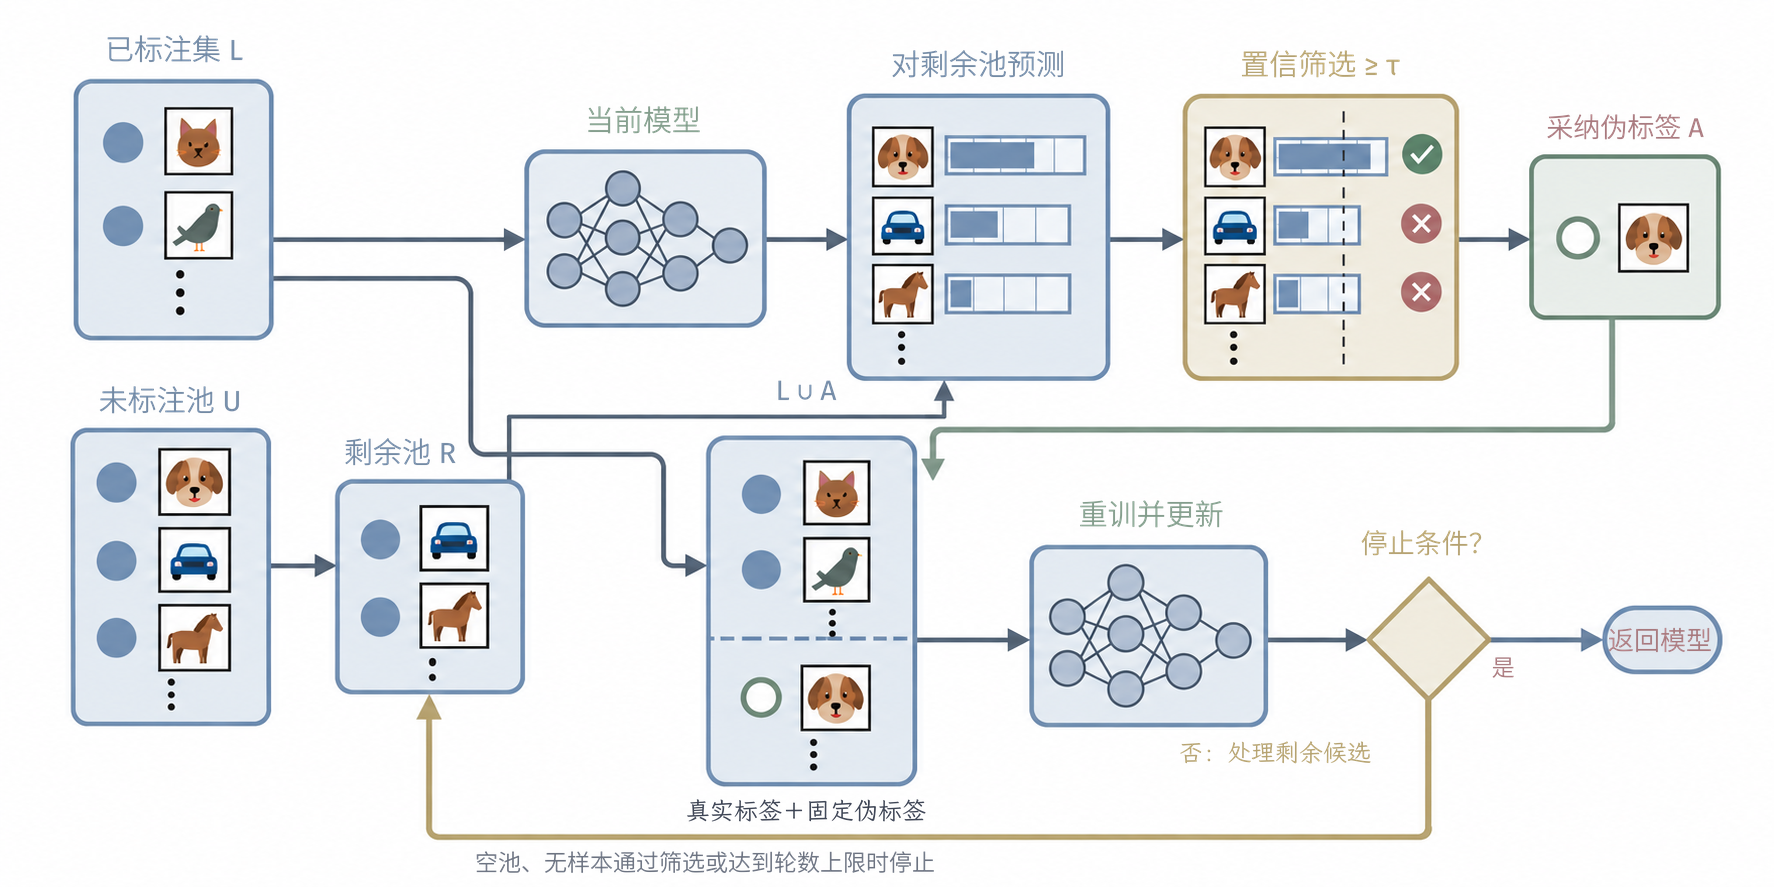
\includegraphics[width=150.199mm]{figures/03-models/01-classic-models/generated/classification-self-training/figure.png}
  \caption{固定阈值、固定已采纳伪标签的自训练流程，对应算法~\ref{alg:classification-self-training}。真实标签保持不变，已采纳的伪标签始终是模型预测。每次采纳后先重训，再用更新后的模型处理剩余候选；空池、无样本通过筛选或达到轮数上限时停止。这个模型反馈回路也可能产生确认偏差：错误预测被当作后续监督，使模型进一步强化原有误判。}
  \label{fig:classification-self-training}
\end{figure*}

每轮也可以在通过阈值的样本中只取前若干项，限制一次扩充的影响；按类别限制数量则可避免易预测类别占据全部新增监督。这些策略改变$B^{(t)}$的构造，集合更新仍按保存标签、扩充集合、重训的顺序执行。类别配额依据任务中的类别比例设置。

\subsubsection{理论分析}
\label{sec:classification-self-training-analysis}

\paragraph{表达能力}
自训练的候选空间仍主要由基分类器决定，伪标签改变训练信号和实际选解。若基分类器无法表达目标边界，反复扩充不会自动解决这个缺口。

\paragraph{收敛性}
这个基本版本何时停止，可以直接从集合变化判断。每次成功扩充至少从$R$移走一个样本，且样本不会移回，因此成功扩充最多发生$\min\{T,|U|\}$次；若没有样本通过筛选，循环会更早结束。只要每次基分类器训练能够返回，外层循环就会有限终止。这一保证针对集合扩充过程的有限终止；各轮训练集和监督信号发生变化，参数优化与统计风险需针对相应模型另行分析。

自训练与\term{熵最小化}（entropy minimization）有共同的倾向：都可能让未标注样本上的预测变得更确定。熵最小化直接惩罚模型预测分布的条件熵，推动概率集中到少数类别。Grandvalet与Bengio讨论了这一准则及其与自训练的联系，这种联系依赖具体的概率模型、筛选和优化设置\scite{grandvalet2004entropy}。

对一个未标注输入$\bm{x}$，Shannon熵与硬伪标签交叉熵分别涉及
\begin{equation}
  \label{eq:classification-pseudolabel-entropy}
  \begin{aligned}
    H_{\bm{\theta}}(\bm{x})
      &=-\sum_{c=1}^{C}p_{\bm{\theta}}(c\mid\bm{x})
        \log p_{\bm{\theta}}(c\mid\bm{x}),\\
    \min_{\widetilde y\in\{1,\dots,C\}}
      \{-\log p_{\bm{\theta}}(\widetilde y\mid\bm{x})\}
      &=-\log\max_c p_{\bm{\theta}}(c\mid\bm{x}).
  \end{aligned}
\end{equation}
前者对所有类别求加权和，后者只取概率最大的一个类别，两者数值和梯度一般不同。例如，预测为$(0.8,0.2)$时，以自然对数计算的熵约为$0.500$，最小硬标签交叉熵约为$0.223$。实际自训练还会筛选样本并冻结历史伪标签，因此下一轮甚至不一定仍以当前最大概率类别为目标。

\paragraph{泛化性}
在同一聚集区域内限制预测差异时，熵最小化倾向于同时提高这些输入的确定性，使边界远离该区域；具体效果依赖基分类器的容量与约束方式。确定性本身仍只描述概率集中程度：若初始模型把同主题文档误判为另一类，采纳后重训可能加强原误判。这种自身错误被重复用作监督的现象称为\term{确认偏差}（confirmation bias）。Arazo等在深度图像分类实验中观察到错误伪标签被拟合，并比较了缓解这一反馈的正则化方法\scite{arazo2020confirmation}。

伪标签错误怎样影响真实风险，可以在固定一轮模型后直接推导。令$h$为这一轮产生伪标签的分类器，$\bm{X}_\tau\subseteq\mathbb{R}^{d}$为通过其置信度阈值的输入区域。对目标分布$\mathcal{P}$，用$R_{\mathcal{P}}(f)=\mathbb{P}_{\mathcal{P}}(f(\bm{x})\ne y)$表示任意候选分类器$f$的新样本风险。设$\pi=\mathbb{P}_{\mathcal{P}}(\bm{x}\in\bm{X}_\tau)>0$，在筛选区域内分别考察伪标签自身的错误率，以及$f$与伪标签不一致的概率：
\begin{equation}
  \label{eq:classification-self-training-conditional-risks}
  \begin{aligned}
    e_\tau
      &=\mathbb{P}_{\mathcal{P}}
        \bigl(h(\bm{x})\ne y\mid\bm{x}\in\bm{X}_\tau\bigr),\\
    \widetilde R_\tau(f)
      &=\mathbb{P}_{\mathcal{P}}
        \bigl(f(\bm{x})\ne h(\bm{x})\mid\bm{x}\in\bm{X}_\tau\bigr).
  \end{aligned}
\end{equation}
若$f$预测错误，它要么与$h$不一致，要么沿用了$h$的错误，因此
\begin{equation}
  \label{eq:classification-self-training-error-events}
  \{f(\bm{x})\ne y\}
    \subseteq
    \{f(\bm{x})\ne h(\bm{x})\}
    \cup\{h(\bm{x})\ne y\},
\end{equation}
在$\bm{X}_\tau$内应用并集界，再把区域内外的风险相加，得到
\begin{equation}
  \label{eq:classification-self-training-risk}
  \begin{aligned}
    R_{\mathcal{P}}(f)
      \leq{}&\pi\bigl(\widetilde R_\tau(f)+e_\tau\bigr)\\
      &+\mathbb{P}_{\mathcal{P}}
        \bigl(f(\bm{x})\ne y,\ \bm{x}\notin\bm{X}_\tau\bigr).
  \end{aligned}
\end{equation}
式~\eqref{eq:classification-self-training-risk}保留了筛选区的伪标签错误率$e_\tau$与区域外错误。即使$f$完全拟合筛选区的伪标签，这两项仍需控制。这里比较固定一轮模型及其筛选区域上的总体风险；$\widetilde R_\tau(f)$描述总体不一致概率，多轮历史伪标签则由不同模型、不同采纳事件产生。监督泛化分析因此需要考虑这些依赖关系。

提高阈值减少采纳量，系统性的高置信度错误仍可能被保留。伪标签权重与单轮规模控制其训练影响，逐类接受率揭示扩充偏向，保留的真实标签验证集则比较扩充前后的效果。验证样本应独立于反复采纳的训练池。未知类别或监督样本覆盖不足时，还需检查数据组成与筛选区域是否符合任务。

\subsubsection{小结}
\label{sec:classification-self-training-summary}

自训练把已有分类器的部分预测转化为新增监督，适合在保留原有训练和预测接口的情况下探索无标签数据的价值。它的额外成本包括对剩余池反复预测，以及在不断扩大的训练集上重新拟合；基分类器训练昂贵时，这些成本并不小。最终模型仍按原分类器的方式预测新样本，无须保留一个独立的传播图。

自训练需要初始模型筛出可靠且有代表性的样本；标签少到难以支撑这一筛选时，收益也会受限。持续验证与错误处理使其能够适应多轮使用，人工复核则可针对高代价或不确定样本改善标签质量。复核范围与频率由误判代价及标注预算共同确定。

\subsection{Label Propagation}
\label{sec:classification-label-propagation}

自训练通过基分类器决定哪些预测值得采纳；如果可信的信息主要来自样本之间的邻近关系，也可以直接在这些关系上传递标签。\term{标签传播}（label propagation）把样本表示为图的节点，让已有标签沿相似边影响尚无标签的节点。Zhu与Ghahramani在2002年的技术报告中给出了保持已知标签不变的传播方法\scite{zhu2002labelpropagation}。与只在已标注样本中寻找近邻相比，未标注点也参与形成传播路径，使标签能够沿弯曲的高密度区域传递；每轮恢复已知标签，则让它们持续提供监督，不会因反复平均而失去原有的类别信息。

下面用随机游走解释固定标签边界下的传播，软约束版本随后通过另一目标引入。

\subsubsection{模型结构}
\label{sec:classification-label-propagation-structure}

图模型把“哪些输入相似”转化成可计算的边权。令$\mathcal{G}=(V,E,\bm{W})$，其中$V=L\cup U$，$\bm{W}\in\mathbb{R}^{n\times n}$为非负对称权重矩阵，$\bm{W}_{i,j}=\bm{W}_{j,i}\geq0$，且取$\bm{W}_{i,i}=0$。例如，可以先选出近邻边，再在相连节点上使用RBF相似度
\begin{equation}
  \label{eq:classification-label-propagation-weights}
  \bm{W}_{i,j}=
  \begin{cases}
    \exp\bigl(-\gamma\lVert\bm{x}_i-\bm{x}_j\rVert_2^2\bigr),
      & \{i,j\}\in E,\\
    0, & \text{其他情形},
  \end{cases}
\end{equation}
其中$\gamma>0$控制相似度衰减。用$k$近邻关系构图时，单向近邻关系需要经过并集或互近邻等明确规则转成无向边，才能满足对称性。完全图保留所有样本对，稀疏图只保留选中的关系；两者不仅存储成本不同，也可能给出不同的分类结果。

每个节点的加权度记为$\delta_i=\sum_j\bm{W}_{i,j}$，度矩阵满足$\bm{D}_{i,i}=\delta_i$。在所有参与传播的节点度数为正时，定义
\begin{equation}
  \label{eq:classification-label-propagation-transition}
  \bm{P}=\bm{D}^{-1}\bm{W},
  \qquad
  \bm{P}_{i,j}=\frac{\bm{W}_{i,j}}{\delta_i}.
\end{equation}
矩阵$\bm{P}$每行的和为1，表示从一个节点沿边随机走向邻居的转移概率。传播时用这一行权重对邻居的标签信息求平均；权重大，邻居的影响也大。

为了同时处理$C$个类别，令$\bm{F}\in\mathbb{R}^{n\times C}$保存节点得分，$\bm{f}_i=(\bm{F}_{i,1},\dots,\bm{F}_{i,C})^\top$为节点$i$的得分向量。构造同形状的$\bm{Y}$：若$i\in L$，则$\bm{Y}_{i,c}=\mathbb{1}\{y_i=c\}$；若$i\in U$，则整行置零。有标签节点在每轮更新后都恢复到这份独热编码，这种固定边界的操作称为\term{硬钳制}（hard clamping），也就是不允许传播改变已经给定的标签。

标签边界应能沿图到达每个待预测节点。零度无标签节点没有转移概率，完全无标签的连通分量则缺少类别语义；可补充真实标签、按可靠关系重新构图，或对相应节点拒绝预测。孤立的有标签节点保留原标签。自环或微小度数只能调整数值形式，类别信息仍需要标签边界提供。

\subsubsection{参数学习}
\label{sec:classification-label-propagation-learning}

标签传播没有固定维数的分类器参数要拟合，但需要求出全部无标签节点的得分。下面假设零度节点已经处理，每个含无标签节点的连通分量至少含一个有标签节点。把$\bm{F}$按$L$与$U$分成行块$\bm{F}_L=\bm{F}_{L,:}$、$\bm{F}_U=\bm{F}_{U,:}$，并对$\bm{P}$作对应分块。硬钳制意味着$\bm{F}_L^{(t)}=\bm{Y}_L$始终不变，因而只需迭代
\begin{equation}
  \label{eq:classification-label-propagation-iteration}
  \bm{F}_U^{(t+1)}
    =\bm{P}_{U,U}\bm{F}_U^{(t)}
     +\bm{P}_{U,L}\bm{Y}_L.
\end{equation}
右侧第一项传递尚无标签节点之间的当前信息，第二项持续注入真实标签。通常取$\bm{F}_U^{(0)}=\bm{0}$。真实标签在每轮固定为边界，无标签行按该转移式更新。

若迭代达到固定点，移项便得到线性系统与形式上的闭式解
\begin{equation}
  \label{eq:classification-label-propagation-solution}
  \begin{aligned}
    (\bm{I}-\bm{P}_{U,U})\bm{F}_U^\ast
      &=\bm{P}_{U,L}\bm{Y}_L,\\
    \bm{F}_U^\ast
      &=(\bm{I}-\bm{P}_{U,U})^{-1}
        \bm{P}_{U,L}\bm{Y}_L.
  \end{aligned}
\end{equation}
这里$\bm{I}$为$|U|\times|U|$单位矩阵。下一小节将证明，在上述图条件下逆矩阵存在，且任意初始化的迭代都收敛到同一个解。计算时通常直接求解线性系统，避免显式构造逆矩阵。Zhu、Ghahramani与Lafferty给出了这一解的调和函数、图能量和随机游走解释\scite{zhu2003}。

图\ref{fig:classification-label-propagation}给出一个可逐项核算的教学构造，并非实测数据。五个节点依次相连，每条无向边的权重为1；端点1固定属于类1，端点5固定属于类2，节点2、3、4没有标签。令$p_i=\bm{F}_{i,1}^\ast$，由于每个内点恰有两个等权邻居，式~\eqref{eq:classification-label-propagation-iteration}~在固定点处变为
\begin{equation}
  \label{eq:classification-label-propagation-path}
  \begin{aligned}
    p_i&=\frac{p_{i-1}+p_{i+1}}{2},
      &&i=2,3,4,\\
    p_1&=1,\qquad p_5=0.
  \end{aligned}
\end{equation}
内点方程等价于$p_{i+1}-p_i=p_i-p_{i-1}$，所以相邻节点的得分差必须相等。两端总共下降1，分到四条边上，每步下降$1/4$，得到
\[
  (p_1,p_2,p_3,p_4,p_5)
    =(1,0.75,0.5,0.25,0).
\]
类2的得分满足相反的端点条件，故$\bm{f}_i^\ast=(p_i,1-p_i)^\top$。节点2偏向类1，节点4偏向类2；节点3的两类得分相同，按本节“并列时取最小类别编号”的约定判为类1。节点3的类别由并列规则确定，其两类得分所包含的证据仍相同。

\begin{figure}[htbp]
  \centering
  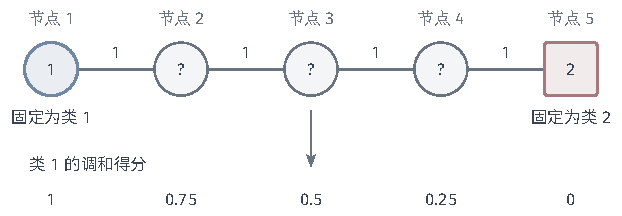
\includegraphics[width=105.315mm]{figures/03-models/01-classic-models/tikz/classification-label-propagation/figure.pdf}
  \caption{五节点等权无向路径上的硬钳制标签传播。每条边权为1，左端圆形节点固定为类1，右端方形节点固定为类2，问号表示未知标签。下方列出精确调和解的类1得分，类2得分为其补数；内点得分等于两侧邻居的平均。中间节点两类并列，按最小类别编号规则判为类1。这是教学构造，不是实测结果。}
  \label{fig:classification-label-propagation}
\end{figure}

迭代实现还需要把停止条件与返回值对应起来。算法\ref{alg:classification-label-propagation}使用相邻两轮之差作为数值停止判据，其中$\lVert\cdot\rVert_{\mathrm{F}}$为Frobenius范数，$\varepsilon>0$为容限，$T\geq1$为最大迭代次数。达到上限时若尚未满足容限，返回状态记录为未收敛，以便解释当前得分的数值精度。

\begin{algorithm}[硬钳制标签传播]
  \label{alg:classification-label-propagation}
  \begin{algorithmic}[1]
    \Require 权重$\bm{W}$、索引$L,U$、标签矩阵$\bm{Y}$
    \Require 容限$\varepsilon>0$、最大迭代次数$T\geq1$
    \Ensure 得分$\bm{F}$、预测$\widehat{\bm{y}}_U$及停止状态
    \If{$U=\varnothing$}
      \State \Return $\bm{Y}$、空预测、已完成
    \EndIf
    \State 检查$\bm{W}$非负、对称，参与传播的节点度数为正
    \State 检查每个含$U$节点的连通分量至少有一个$L$节点
    \If{任何检查失败}
      \State \Return 拒绝结果，要求补标签或修正传播图
    \EndIf
    \State 构造$\bm{P}=\bm{D}^{-1}\bm{W}$
    \State $\bm{F}_L\gets\bm{Y}_L$，$\bm{F}_U\gets\bm{0}$
    \State $\mathrm{converged}\gets\mathrm{false}$
    \For{$t=1,\dots,T$}
      \State $\bm{G}\gets\bm{P}_{U,U}\bm{F}_U+\bm{P}_{U,L}\bm{Y}_L$
      \State $\Delta\gets\lVert\bm{G}-\bm{F}_U\rVert_{\mathrm{F}}$
      \State $\bm{F}_U\gets\bm{G}$
      \If{$\Delta\leq\varepsilon(1+\lVert\bm{F}_U\rVert_{\mathrm{F}})$}
        \State $\mathrm{converged}\gets\mathrm{true}$
        \State \textbf{break}
      \EndIf
    \EndFor
    \State $\widehat y_j\gets\argmax_c\bm{F}_{j,c}$，$j\in U$；并列取最小$c$
    \State \Return $\bm{F},\widehat{\bm{y}}_U,\mathrm{converged}$
  \end{algorithmic}
\end{algorithm}

算法先把$\bm{G}$保存成最新的$\bm{F}_U$，再判断是否退出，因此即使本轮达到容限，也会返回新得分而不是上一轮的值。相邻迭代差小是一种可操作的停止指标，不直接给出距离精确解的统一误差界；当传播很慢时，还需结合线性系统残差与条件数判断数值精度。最终类别由得分比较决定，接近平局的节点尤其需要保留得分与未收敛状态。

\subsubsection{理论分析}
\label{sec:classification-label-propagation-analysis}

\paragraph{表达能力}
标签传播把预测限制为与相似图和边界标签相容的平滑函数。真实标签沿强边变化剧烈或图连接错误时，传播偏好可能排除正确划分。

\paragraph{收敛性}
硬钳制传播的收敛来自无标签节点能够沿正权路径到达标签边界。$\bm{P}_{U,U}$的行和至多为1，只有无标签邻居的节点其行和恰为1。因此考察多步后仍留在$U$中的总权重，可以同时处理直接与间接相连的节点。

\begin{theorem}[硬钳制传播的唯一解]
  \label{thm:classification-label-propagation-convergence}
  设图有限、边权非负且对称，所有参与传播的节点度数为正，$U$非空，且每个含无标签节点的连通分量至少含一个有标签节点。则$\rho(\bm{P}_{U,U})<1$，其中$\rho$表示谱半径。式~\eqref{eq:classification-label-propagation-iteration}~从任意初始得分出发，都收敛到式~\eqref{eq:classification-label-propagation-solution}~中的唯一固定点。
\end{theorem}

\begin{proof}
  从每个$j\in U$出发，选择一条到达$L$的正权路径，并在首次到达$L$时停止。有限图中这些路径长度有一个共同上界$m$，沿各路径行走的概率均为正，其最小值记为$\epsilon>0$。于是，无论从哪个无标签节点出发，在$m$步以内命中$L$的概率都至少为$\epsilon$。这说明
  \[
    \lVert\bm{P}_{U,U}^{m}\rVert_\infty\leq1-\epsilon,
    \qquad
    \rho(\bm{P}_{U,U})^m\leq1-\epsilon<1.
  \]
  因而$\bm{P}_{U,U}^t$趋于零，Neumann级数收敛，且
  \[
    (\bm{I}-\bm{P}_{U,U})^{-1}
      =\sum_{t=0}^{\infty}\bm{P}_{U,U}^{t}.
  \]
  迭代展开为
  \[
    \bm{F}_U^{(t)}
      =\bm{P}_{U,U}^{t}\bm{F}_U^{(0)}
       +\sum_{s=0}^{t-1}
         \bm{P}_{U,U}^{s}\bm{P}_{U,L}\bm{Y}_L.
  \]
  第一项消失，第二项趋于所述固定点。逆矩阵存在，也排除了其他固定点。
\end{proof}

还可以从最优化的角度解释同一个解。相邻节点的得分差越大，图上的不平滑程度越高。令$\bm{L}_{\mathrm{g}}=\bm{D}-\bm{W}$为\term{图拉普拉斯矩阵}（graph Laplacian），它把这种局部差异汇总成二次型。固定真实标签边界后，求解的\term{Dirichlet能量}（Dirichlet energy）最小化问题为
\begin{equation}
  \label{eq:classification-label-propagation-energy}
  \begin{aligned}
    \min_{\bm{F}:\,\bm{F}_L=\bm{Y}_L}\quad
    \mathcal{E}(\bm{F})
      &=\frac12\sum_{i,j=1}^{n}
        \bm{W}_{i,j}\lVert\bm{f}_i-\bm{f}_j\rVert_2^2\\
      &=\operatorname{tr}
        (\bm{F}^{\top}\bm{L}_{\mathrm{g}}\bm{F}).
  \end{aligned}
\end{equation}
第\ref{sec:clustering-spectral}节的谱聚类与第\ref{sec:dim-le}节的拉普拉斯特征映射复用图拉普拉斯和谱工具，但输出分别是离散簇分配与连续低维坐标；这里的标签传播则在已知类别语义下求类别得分。三种任务分别对类别得分、簇分配和坐标施加输出约束。

有标签节点固定为边界，优化变量只包含无标签行。对未知行块求导并令其为零，得到
\begin{equation}
  \label{eq:classification-label-propagation-dirichlet}
  \begin{aligned}
    (\bm{L}_{\mathrm{g}})_{U,U}\bm{F}_U
      &=-(\bm{L}_{\mathrm{g}})_{U,L}\bm{Y}_L\\
      &=\bm{W}_{U,L}\bm{Y}_L.
  \end{aligned}
\end{equation}
因为$(\bm{L}_{\mathrm{g}})_{U,U}=\bm{D}_{U,U}-\bm{W}_{U,U}$，左乘$\bm{D}_{U,U}^{-1}$就回到式~\eqref{eq:classification-label-propagation-solution}~的线性系统。

这个驻点也是唯一最小值，而不只是一个形式上的导数解。取任意无标签节点上的非零向量$\bm{z}$，把它扩展成在$L$上为零的全图向量$\widetilde{\bm{z}}$，则
\[
  \bm{z}^{\top}(\bm{L}_{\mathrm{g}})_{U,U}\bm{z}
    =\frac12\sum_{i,j}\bm{W}_{i,j}
      (\widetilde z_i-\widetilde z_j)^2.
\]
右侧若为零，向量在每个正权连通分量上就必须为常数。每个涉及$U$的分量又含一个值为零的标签边界，因此这些常数只能全部为零，与$\bm{z}\ne\bm{0}$矛盾。故未标记主子块正定，能量对$\bm{F}_U$严格凸。这同时解释了为什么完全无标签的分量会破坏唯一性：在这种分量上，任意常值向量都不增加图能量。

得分的概率含义也需要依赖这些条件。从一个无标签节点按$\bm{P}$行走，并在首次碰到有标签节点时停止，$\bm{F}_{j,c}^\ast$等于首次命中的标签属于类$c$的概率。由于最终命中$L$的概率为1，精确解各行非负且行和为1。若从零初始化，有限轮得分只累积了相应步数内的命中概率，行和可能还小于1；一般不能把尚未收敛的得分直接当成归一化概率。即便在极限处，这也是给定图上的命中概率，不自动等于真实任务中校准的类别后验。

\paragraph{泛化性}
图的统计意义取决于相似关系是否符合类别。\term{平滑假设}（smoothness assumption）要求强边连接的节点具有相近标签得分；文档按写作风格聚集、任务却按主题分类时，这一联系可能失效。跨类强边传播错误信息，错误边界标签还会在每轮持续注入。特征标准化、降维或度量学习可改变高维构图的表示，选择后的图仍需用真实标签验证。

这里还要区分两种评价对象。对非空$U$，在训练之外取得真实标签后，可以计算
\begin{equation}
  \label{eq:classification-label-propagation-pool-risk}
  \widehat R_U
    =\frac{1}{|U|}\sum_{j\in U}
      \mathbb{1}\{\argmax_c\bm{F}_{j,c}^\ast\ne y_j\}.
\end{equation}
其中并列得分仍按最小类别编号处理，$y_j$只用于评价。这个误差评价已经参与构图的输入，未来独立样本需使用另行定义的预测规则。要讨论新样本，还必须定义归纳扩展$h_{\mathcal{G}}(\bm{x})$，即规定新输入如何连接到图、怎样由图上得分产生预测，以及是否重新求解；这时才有相应的风险$R_{\mathcal{P}}(h_{\mathcal{G}})=\mathbb{P}_{\mathcal{P}}(h_{\mathcal{G}}(\bm{x})\ne y)$。

前述唯一解定理确定给定图上的得分。要控制$R_{\mathcal{P}}(h_{\mathcal{G}})$，还需规定归纳扩展，并将构图规则、标签覆盖与类别平滑性联系到目标分布；这些统计条件使给定图上的求解结果具有新样本风险解释。

\subsubsection{小结}
\label{sec:classification-label-propagation-summary}

标签传播适合相似关系本身可信的任务，例如有可靠连接语义的节点分类，或用局部外观关系传播图像块标签。其基本输出是当前图上各节点的得分，适合面向这批输入作出预测；若任务持续接收新输入，前述归纳扩展也应纳入模型设计和评价。

图的稀疏性与求解精度共同决定计算成本。记$\operatorname{nnz}(\bm{W})$为非零权重数，稀疏图一次传播的主要乘法成本为$O(\operatorname{nnz}(\bm{W})C)$，存储主要为$O(\operatorname{nnz}(\bm{W})+nC)$；总时间还要乘以迭代次数，并另计构图成本。完全图的存储为$O(n^2)$，直接计算所有欧氏距离通常需$O(n^2d)$。即使图很稀疏，连接标签区域的边过弱，也会使$\rho(\bm{P}_{U,U})$接近1，导致传播缓慢。

可以利用稀疏线性求解器，或在合适的相似度矩阵上使用\term{Nyström近似}（Nyström approximation），即选取少量代表列来构造低秩近似，减少矩阵运算。但近似相似度不一定保留原图的非负边权、连通关系与硬边界解；采用近似后应重新检查这些条件和求解误差。图上的唯一解、数值上的近似精度以及分类准确率，是三个需要分别评价的问题。

\subsection{TSVM}
\label{sec:classification-tsvm}

图传播直接平滑节点得分；若希望保留SVM的分类函数，则可以让无标签样本参与选择大间隔边界。\term{直推支持向量机}（transductive support vector machine, TSVM）同时选择分类器与当前未标注样本的标签，使两类样本共同约束间隔。Joachims在1999年的文本分类研究中给出了有代表性的目标与实用求解算法。其相关性反馈任务说明了这一选择的背景：用户只标注少量检索结果是否相关，其余待分类文档却已经构成一个给定的文档库。于是，这些文档不必等到训练结束后才交给分类器，而可以在训练时通过自身的位置参与确定间隔边界\scite{joachims1999transductive}。

这里的\term{直推学习}（transductive learning，也称转导学习）指利用当前已给定的待预测输入，直接推断这批输入的标签；它与面向未来新输入评价预测规则的归纳设定有所区别。TSVM仍会得到一个SVM分类函数，所以从计算上也能处理新样本。两种评价设定的差异在于参与训练的输入及风险针对的预测集合。

\subsubsection{模型结构}
\label{sec:classification-tsvm-structure}

本小节使用二分类标签$\{-1,+1\}$。令$g(\bm{x})=\bm{w}^{\top}\phi(\bm{x})+b$为决策分数，$\phi$为选定的特征映射；线性SVM取$\phi(\bm{x})=\bm{x}$。标准软间隔SVM只要求已标注样本尽量满足$y_i g(\bm{x}_i)\geq1$。TSVM还为每个$j\in U$引入一个待选择的离散标签$y_j^{\mathrm{u}}$，并为相应间隔约束配置松弛变量$\xi_j^{\mathrm{u}}$。其目标可写为
\begin{equation}
  \label{eq:classification-tsvm-objective}
  \begin{aligned}
    \min_{\bm{w},b,\bm{y}^{\mathrm{u}},\bm{\xi}}\quad
    \mathcal{J}
      ={}&\frac12\lVert\bm{w}\rVert_2^2
         +\lambda_{\mathrm{s}}\sum_{i\in L}\xi_i\\
       &+\lambda_{\mathrm{u}}\sum_{j\in U}\xi_j^{\mathrm{u}},
  \end{aligned}
\end{equation}
其中$\bm{y}^{\mathrm{u}}$收集无标签节点的离散标签，$\bm{\xi}$收集两类松弛变量，$\lambda_{\mathrm{s}}>0$与$\lambda_{\mathrm{u}}\geq0$分别控制有标签项和无标签项的惩罚。约束为
\begin{equation}
  \label{eq:classification-tsvm-constraints}
  \begin{aligned}
    y_i g(\bm{x}_i)&\geq1-\xi_i,
      &\xi_i&\geq0,\quad i\in L,\\
    y_j^{\mathrm{u}}g(\bm{x}_j)&\geq1-\xi_j^{\mathrm{u}},
      &\xi_j^{\mathrm{u}}&\geq0,\quad j\in U,\\
    y_j^{\mathrm{u}}&\in\{-1,+1\},
      &&j\in U,\\
    \sum_{j\in U}\frac{1+y_j^{\mathrm{u}}}{2}&=r.
  \end{aligned}
\end{equation}
最后一行固定无标签样本中的正类标签数量$r$。本节讨论$|U|\geq2$且$1\leq r\leq|U|-1$的非退化情形；$\lambda_{\mathrm{u}}=0$或$U$为空时，分类器训练回到纯监督SVM。

类别数量约束来自一个实际困难：无标签样本本身不能说明哪一侧应有多少样本。若只要求间隔大，模型可能把几乎全部未标注样本放到同一类，从而得到不符合任务的划分。\term{类别平衡约束}（class-balance constraint）把对类别组成的外部知识加入优化，它不要求两类数量相等，而是固定或限制可接受的比例。可以根据可信先验选择$r$，也可以规定$r_{\min}\leq\sum_j(1+y_j^{\mathrm{u}})/2\leq r_{\max}$。由少量已标注样本估计比例时，需要考虑抽样偏差；错误的比例约束同样会损害结果。

数量约束固定待优化标签中的正类数。松弛变量仍允许分类器误分样本或使其落在间隔内，因此标签交换可以保持可行标签数，而重训后的正预测数可能变化。

无标签项怎样影响边界，可以暂时去掉数量约束来观察。对给定分数$s$，若允许独立选择二分类标签，最小的无标签合页损失为
\begin{equation}
  \label{eq:classification-tsvm-unlabeled-hinge}
  \min_{y\in\{-1,+1\}}[1-ys]_+=[1-|s|]_+,
\end{equation}
其中$[a]_+=\max\{a,0\}$。这项损失惩罚分数靠近零的无标签样本，却不预先规定它们应落在哪一侧。在合适的表示下，若大量输入集中在少数区域，让边界避开这些区域就能减少此项损失。这是\term{低密度分离假设}（low-density separation assumption）的作用：类别分界应经过输入较少的区域，而不是切开高密度的同类区域。恢复类别数量约束后，各个标签选择相互耦合，不能再逐样本独立最小化。

\subsubsection{参数学习}
\label{sec:classification-tsvm-learning}

固定$\bm{y}^{\mathrm{u}}$以后，式~\eqref{eq:classification-tsvm-objective}~就是具有不同样本惩罚的软间隔SVM，可以沿用相应凸优化求解器。困难在于标签本身还要选择：固定正类数$r$时有$\binom{|U|}{r}$种标签配置，通常无法逐一求解比较。实用算法从监督SVM出发，交替改善标签与分类器，并逐步提高$\lambda_{\mathrm{u}}$，使无标签数据的影响从弱变强。

初始化也要满足数量约束。先在$L$上训练监督SVM，按它对$U$的决策分数排序，把分数最高的$r$个样本暂定为正类，其余为负类；分数并列时按样本索引排序。监督分类器的正负预测数可能不同于$r$，排序初始化则使数量约束从第一轮开始成立。

在固定$\lambda_{\mathrm{u}}>0$的一轮内，可以交换一个当前正类样本$a$与负类样本$b$的标签。这样正类总数不变，只需判断交换是否有利。记$\ell_{\mathrm{h}}(s)=[1-s]_+$，在当前分类器分数不变时，交换带来的无标签损失变化为
\begin{equation}
  \label{eq:classification-tsvm-swap}
  \begin{aligned}
    \Delta_{a,b}
      ={}&\ell_{\mathrm{h}}\bigl(-g(\bm{x}_a)\bigr)
          +\ell_{\mathrm{h}}\bigl(g(\bm{x}_b)\bigr)\\
       &-\ell_{\mathrm{h}}\bigl(g(\bm{x}_a)\bigr)
          -\ell_{\mathrm{h}}\bigl(-g(\bm{x}_b)\bigr).
  \end{aligned}
\end{equation}
若$\Delta_{a,b}<0$，仅交换标签并相应调整松弛变量，就已经降低了目标中的无标签项；随后重新求解固定标签的SVM，目标值只会进一步降低或保持不变。这个判据识别在当前得分下即可降低损失的交换，搜索范围因此限定于这类变化。

算法\ref{alg:classification-tsvm}采用这一下降判据说明求解过程。$\operatorname{FitSVM}(\bm{y}^{\mathrm{u}},\lambda_{\mathrm{u}})$表示在当前固定标签下，用有标签惩罚$\lambda_{\mathrm{s}}$和无标签惩罚$\lambda_{\mathrm{u}}$完整求解SVM。原始实现还可以为未标注正负类使用不同惩罚；这里用统一的$\lambda_{\mathrm{u}}$突出类别平衡、交换与逐步加权的关系。

\begin{algorithm}[固定类别数量的TSVM逐步加权]
  \label{alg:classification-tsvm}
  \begin{algorithmic}[1]
    \Require 含两个类别的训练索引$L$，无标签索引$U$
    \Require $|U|\geq2$，正类数量$1\leq r\leq|U|-1$
    \Require $\lambda_{\mathrm{s}}>0$，目标$\lambda_{\mathrm{u}}^{\mathrm{final}}>0$
    \Require 初值$\lambda_{\mathrm{u}}^{(0)}>0$，倍率$q>1$，容限$\varepsilon\geq0$
    \Ensure 分类器$g$及离散标签$\bm{y}^{\mathrm{u}}$
    \State 在$L$上训练监督SVM，得到$g$
    \State 按$g$的分数将$U$中前$r$个样本标为正，其余标为负
    \State $\lambda_{\mathrm{u}}\gets
      \min\{\lambda_{\mathrm{u}}^{(0)},\lambda_{\mathrm{u}}^{\mathrm{final}}\}$
    \While{尚未在目标惩罚值下完成训练}
      \State $g\gets\operatorname{FitSVM}(\bm{y}^{\mathrm{u}},\lambda_{\mathrm{u}})$
      \While{存在正负标签对$(a,b)$使$\Delta_{a,b}<-\varepsilon$}
        \State 交换$y_a^{\mathrm{u}}$与$y_b^{\mathrm{u}}$
        \State $g\gets\operatorname{FitSVM}(\bm{y}^{\mathrm{u}},\lambda_{\mathrm{u}})$
      \EndWhile
      \If{$\lambda_{\mathrm{u}}=\lambda_{\mathrm{u}}^{\mathrm{final}}$}
        \State \textbf{break}
      \EndIf
      \State $\lambda_{\mathrm{u}}\gets
        \min\{q\lambda_{\mathrm{u}},\lambda_{\mathrm{u}}^{\mathrm{final}}\}$
    \EndWhile
    \State \Return $g,\bm{y}^{\mathrm{u}}$
  \end{algorithmic}
\end{algorithm}

逐步增加无标签惩罚常称为\term{退火}（annealing）：先在真实标签主导的目标上取得初始解，再逐渐增加无标签约束的影响。这里的每个阶段都先训练并完成交换搜索，再判断是否已经达到最终惩罚值。惩罚更新到目标值后，还需在该值下完成训练与交换搜索，才能返回对应模型。若另设总时间或阶段数量上限，应把提前终止作为未完成目标惩罚训练的状态返回。

这一过程使用上一阶段的结果作初始化，可视为一种延续求解策略，但离散标签变化可能使解发生跳变，不保证存在一条光滑的解路径。退火倍率、初始标签和交换搜索方式会改变最终结果，因此可用多个合理初始化与独立验证比较局部搜索结果。

\subsubsection{理论分析}
\label{sec:classification-tsvm-analysis}

\paragraph{表达能力}
TSVM在所选线性或核得分族中寻找低密度分界，未标注数据改变边界偏好。目标若穿过高密度区域，低密度假设反而可能排除合适候选。

\paragraph{收敛性}
固定标签子问题的凸性，不会使标签与参数联合优化也变凸。式~\eqref{eq:classification-tsvm-unlabeled-hinge}~已经显示出其中的非凸性：在$s=-1$和$s=1$处损失均为零，在中点$s=0$处却为1，不满足凸函数的中点不等式。实际问题又包含离散标签及其数量限制，因而是连续变量与离散变量耦合的非凸优化问题。求解一个固定标签的SVM与搜索标签配置，是两项不同的工作。

在固定惩罚值下，算法的有限终止可以有一个明确但有限的保证。假设每次固定标签的SVM都求到全局最小值，并且只接受式~\eqref{eq:classification-tsvm-swap}~所给出的严格下降交换。令$V(\bm{y}^{\mathrm{u}})$为当前标签配置对应的最优目标值，则一次接受交换后有
\[
  V(\bm{y}_{\mathrm{new}}^{\mathrm{u}})
    \leq V(\bm{y}_{\mathrm{old}}^{\mathrm{u}})
      +\lambda_{\mathrm{u}}\Delta_{a,b}
    <V(\bm{y}_{\mathrm{old}}^{\mathrm{u}}).
\]
可行标签配置有限，因此不能在严格下降过程中反复回到同一配置，内层搜索最终会停止。倍率$q>1$并在目标值处截断，也保证外层惩罚阶段有限。这一结论依赖精确子问题求解与严格下降；使用数值近似时，需要检查重训后的实际目标变化，不能只根据理想化推导接受任意交换。

停止只说明当前搜索规则没有找到可接受的改进。即使任何交换在固定$g$时都不下降，也仍可能存在交换后充分重训才改善的解，或者需要同时改变多个标签才能到达的更好配置。因此，这个停止条件既不保证全局最优，也不保证对所有单对交换重训都已最优。不同$\lambda_{\mathrm{u}}$阶段之间的目标函数也不同，跨阶段的目标值不构成同一目标下的下降序列。

\paragraph{泛化性}
统计上的风险来自另一组条件。如果两个真实类别在同一高密度区域内严重重叠，正确的分类边界可能就需要穿过该区域。较大的$\lambda_{\mathrm{u}}$却会奖励避开它的边界，导致无标签数据拉低分类性能。错误的类别比例、未标注池中的未知类别，以及只对局部区域可靠的初始监督模型，也可能产生类似损害。优化更充分并不能修复失效的分布假设，有时反而会更彻底地实现一个不适合任务的目标。

TSVM与监督SVM比较时，固定特征、有标签训练集及评价数据。直推实验允许当前待预测输入参与训练，结果评价这批输入；用于未来输入时，则在独立新样本上另行检验归纳预测。两种设定都使用未参与调参的真实标签计算错误。

一种不依赖TSVM优化过程的检查，是在训练与调参全部完成后，固定最终分类规则$f$，再用$m\geq1$个独立来自目标分布$\mathcal{P}$的真实标注测试样本评价。这些样本的输入也不参与训练、特征拟合或模型选择。记其零一测试误差为$\widehat R_{\mathrm{test}}(f)$；条件于训练所得的$f$，每个测试错误都是均值为$R_{\mathcal{P}}(f)$的独立Bernoulli变量。由
\BookEquationRef{eq:hoeffding-fixed-hypothesis}{第二卷“基础、理论和可信性”的“二分类学习的可学习性”章中的Hoeffding不等式}，
对$0<\delta<1$，至少以$1-\delta$的概率有
\begin{equation}
  \label{eq:classification-semisupervised-test-risk}
  R_{\mathcal{P}}(f)
    \leq\widehat R_{\mathrm{test}}(f)
       +\sqrt{\frac{\log(2/\delta)}{2m}}.
\end{equation}
该界把最终固定规则的独立测试误差联系到新样本风险，也适用于自训练分类器或已定义归纳扩展的图分类器。$m$计数独立测试样本，半监督方法是否优于基线仍需同条件比较。若依据这批测试结果继续选择模型，需加入选择校正或保留新的独立测试集。

\subsubsection{小结}
\label{sec:classification-tsvm-summary}

TSVM保留了SVM的决策函数，把变化集中在训练目标与离散标签搜索中。预测新输入时仍计算$g(\bm{x})$并取其符号；分数恰为零时，应使用预先约定的并列规则。它适用于大间隔与低密度分离有合理联系、类别组成可约束的任务，无标签样本的价值由这些结构联系决定。

TSVM的训练成本来自带权SVM求解与标签交换，受核矩阵、基求解器、惩罚阶段和搜索策略影响。数量约束排除部分退化配置，逐步加权利用前一阶段结果作初始化。准确率收益仍依赖分离假设；后面的安全半监督方法进一步按候选划分控制可能损害。

\subsection{模型对比与总结}
\label{sec:classification-semisupervised-comparison}

自训练、标签传播与TSVM使用同一类额外资源——未标注输入，却分别提取补充监督、关系平滑与边界位置信息。表\ref{tab:classification-semisupervised-comparison}加入生成式EM，与前面的概率分类模型相连。后续的多视图训练、软传播、流形正则化与安全选择继续改变监督来源或约束方式，这些机制可以结合使用。

\begin{table}[htbp]
  \centering
  \small
  \begin{tabularx}{\linewidth}{@{}>{\RaggedRight\arraybackslash}p{25mm}>{\RaggedRight\arraybackslash}X>{\RaggedRight\arraybackslash}X@{}}
    \toprule
    方法 & 无标签数据怎样参与 & 关键条件与代价 \\
    \midrule
    Self-Training & 筛选预测作伪标签，反复训练原分类器 & 采纳的预测应可靠；需反复预测与重训，警惕确认偏差。 \\
    Label Propagation & 在固定标签边界下求图上调和得分 & 图应反映类别关系，且无标签分量能到达标签；成本依赖边数与求解精度。 \\
    TSVM & 联合选择离散标签与大间隔分类器 & 低密度分离及类别数量约束应合理；需要非凸标签搜索与多次SVM训练。 \\
    生成式EM & 把未知类别视为潜变量，按类别软后验累计期望统计量 & 联合模型应足够贴合输入与类别；EM只保证相应似然的局部改进。 \\
    \bottomrule
  \end{tabularx}
  \caption{四种半监督分类机制的比较。表中列的是使用信息的方式与主要限制，不构成准确率或计算复杂度从低到高的排序。前三行对应本节完整展开的模型，生成式EM行提供与概率分类模型相连的最小入口。}
  \label{tab:classification-semisupervised-comparison}
\end{table}

生成式半监督方法从另一条路线利用未标注输入。设联合模型为$p_{\bm{\theta}}(\bm{x},y)$，有标签样本直接贡献输入与类别的联合对数似然，未标注样本则只贡献输入的边缘对数似然：
\[
  \ell(\bm{\theta})
  =\sum_{i\in L}\log p_{\bm{\theta}}(\bm{x}_i,y_i)
   +\sum_{j\in U}\log\sum_{c=1}^{C}
      p_{\bm{\theta}}(\bm{x}_j,c).
\]
在这个模型中，全部输入与全部类别合称\term{完全数据}（complete data），其中包括实际未观测的类别；这里的“完全”指连同潜类别一并规定的随机变量。EM在训练时把$U$中的未知类别作为潜变量处理。E步用当前参数计算软后验$q_j(c)=p_{\bm{\theta}^{(t)}}(y=c\mid\bm{x}_j)$；M步最大化当前软后验下的期望完全数据对数似然。记
\[
  \begin{aligned}
    Q(\bm{\theta}\mid\bm{\theta}^{(t)})
    &=
    \sum_{i\in L}\log p_{\bm{\theta}}(\bm{x}_i,y_i) \\
    &\quad+
    \sum_{j\in U}\sum_{c=1}^{C}
      q_j(c)\log p_{\bm{\theta}}(\bm{x}_j,c), \\
    \bm{\theta}^{(t+1)}
    &\in\argmax_{\bm{\theta}}
      Q(\bm{\theta}\mid\bm{\theta}^{(t)}).
  \end{aligned}
\]
只有对多项式NB这类以类别与类别词频为充分统计量的模型，M步才可以解释为把$q_j(c)$作为分数类别计数，与真实标签统计量一起更新先验和类条件参数。此时，未标注文档的词频按$q_j(c)$分配给各类别，而不是先固定成一个不可更改的硬伪标签。Nigam等在文本分类中给出了这一路线的代表性实现\scite{nigam2000text}。

\Needspace{14\baselineskip}
精确E步和充分求解的M步保证相应观测似然不下降\scite{clust-dempster1977}。这一结论只针对选定生成模型和当前局部解，不能推出分类风险必然下降。模型失配时，大量未标注输入会加强对错误边缘结构的拟合，甚至使分类性能劣于只使用标签的基线；Cozman与Cohen给出了这一现象的直接分析与实验\scite{cozman2002unlabeled}。当潜变量不止类别，或后验不能闭式计算时，还需要结合具体图结构选择精确或近似推断；第\ref{part:probabilistic-models}部分提供概率图模型的统一语境，本节不展开这些推断细节。

计算预算取决于每种操作的具体规模：自训练反复拟合基分类器，图传播承担构图与稀疏求解，TSVM进行多阶段SVM训练，生成式EM反复计算后验并更新统计量。样本数、特征维数、类别数、边数与迭代次数共同决定成本。已有可靠分类器时可尝试自训练，可信关系图支持标签传播，间隔与低密度联系支持TSVM，可信联合模型及可计算软统计量支持EM；收益均在相同评价条件下与监督基线比较。

自训练的一个薄弱处是同一个模型既提出标签，又把它们作为后续训练依据。如果输入天然具有两种互补描述，可以让不同视图的模型提供监督。\term{协同训练}（co-training）分别在两个视图上训练分类器，再让一个分类器选出的高置信度标签供另一个使用。Blum与Mitchell在1998年的研究中使用网页正文与指向该网页的链接文字作为两种描述；其理论设定包括每个视图都足以确定类别，以及给定类别后两视图条件独立\scite{blum1998cotraining}。

视图充分性使单个模型有可能完成分类，条件独立性限制两视图共享错误的方式。若视图存在同一种偏差，互供伪标签仍会强化错误；相关视图或人工划分视图的任务可用独立验证考察效果，其理论分析需按实际视图关系重新建立。

没有两种天然视图时，也可以通过重采样构造多个分类器。\term{三训练}（tri-training）使用三个模型，并让其中两个的一致预测为第三个提供候选伪标签。Zhou与Li在2005年提出的方法用bootstrap样本初始化模型，三个分类器可以使用相同特征和相同学习算法；最终预测通过三者投票得到\scite{zhou2005tritraining}。

三训练中的一致意见只是候选生成条件。原算法还利用有标签数据估计两个“提供标签”的模型在一致样本上的错误情况，并结合候选数量控制新增监督的错误负担；必要时对候选集采样，满足更新条件后才重训接收标签的模型。每个模型使用自己的临时伪标签集，与原始有标签集结合训练，而不是把所有一致预测永久变成真实标签。重采样制造的差异能否带来有用互补，仍受样本覆盖与模型错误相关性影响。

图方法的另一项选择是是否始终保留原标签。硬钳制适合把标签视为可信边界，但标签本身有噪声时，可能希望邻域信息也能调整有标签节点。Zhou等人在2003年的局部与全局一致性方法中给出了软约束传播及其正则化解释\scite{zhou2003consistency}。这类\term{标签扩散}（label spreading）方法使节点在邻域平滑与贴近初始标签之间折中。

在所有节点度数为正的非负对称图上，定义
\begin{equation}
  \label{eq:classification-label-spreading-matrices}
  \bm{S}=\bm{D}^{-1/2}\bm{W}\bm{D}^{-1/2},
  \qquad
  \bm{L}_{\mathrm{sym}}=\bm{I}-\bm{S}.
\end{equation}
$\bm{S}$是对称归一化邻接矩阵，$\bm{L}_{\mathrm{sym}}$才是对称归一化拉普拉斯矩阵。$\bm{S}$的特征值位于$[-1,1]$，但不一定非负：两个节点以一条边相连时，$\bm{S}$的特征值就是$1$和$-1$。因此，支撑正则化目标凸性的是$\bm{L}_{\mathrm{sym}}$的半正定性，而不是$\bm{S}$半正定。

沿用未标记行置零的初始矩阵$\bm{Y}$，软约束目标为
\begin{equation}
  \label{eq:classification-label-spreading-objective}
  \min_{\bm{F}}\quad
    \operatorname{tr}
      (\bm{F}^{\top}\bm{L}_{\mathrm{sym}}\bm{F})
    +\mu\lVert\bm{F}-\bm{Y}\rVert_{\mathrm{F}}^2,
  \qquad \mu>0.
\end{equation}
第一项约束按度数归一化后的得分在图上平滑，第二项覆盖全部节点，而不只覆盖$L$。在未标记节点上，$\bm{Y}$为零，所以这一项也在约束得分大小。对目标求导并令其为零，得到$[(1+\mu)\bm{I}-\bm{S}]\bm{F}=\mu\bm{Y}$。令$\alpha=1/(1+\mu)$，则
\begin{equation}
  \label{eq:classification-label-spreading-fixed-point}
  \begin{aligned}
    \bm{F}^{(t+1)}
      &=\alpha\bm{S}\bm{F}^{(t)}+(1-\alpha)\bm{Y},\\
    \bm{F}^\ast
      &=(1-\alpha)(\bm{I}-\alpha\bm{S})^{-1}\bm{Y}.
  \end{aligned}
\end{equation}
由于$0<\alpha<1$且$\rho(\bm{S})\leq1$，有$\rho(\alpha\bm{S})<1$，这一次收敛来自显式收缩系数。迭代中所有节点都按同一公式更新，有标签行也不再恢复成$\bm{Y}_L$。重新施加硬钳制后，优化问题改变，需按固定边界重新求解。

$\alpha$增大时，图平滑相对于标签拟合的作用增强，某些含噪标签可以被邻居信息修正，也可能把本来正确的少数类标签过度平滑。软得分的行和通常不等于1；按行归一化可以服务于展示或分类接口，但不会自动得到校准概率。完全没有标签的分量在这个软目标下会得到零解，数值上的唯一性仍未赋予它类别信息。因此，软约束的灵活性要与标签噪声和图质量一同评价。

如果希望同时使用图结构并直接预测新输入，可以把图能量施加在分类函数上。\term{拉普拉斯支持向量机}（Laplacian SVM）在监督合页损失之外加入图正则项，要求相似样本上的函数值接近。

以下讨论二分类，将有标签样本的类别编码为$y_i\in\{-1,+1\}$。设$g$属于核$K$的再生核Hilbert空间$\mathcal{H}_K$，$b$为偏置，$\bm{s}$收集全部样本的分数$s_i=g(\bm{x}_i)+b$。采用与本章SVM一致的惩罚记号，一种相应目标是
\begin{equation}
  \label{eq:classification-laplacian-svm}
  \begin{aligned}
    \min_{g\in\mathcal{H}_K,b}\quad
      &\frac12\lVert g\rVert_{\mathcal{H}_K}^2
       +\lambda_{\mathrm{s}}\sum_{i\in L}[1-y_i s_i]_+\\
      &+\frac{\lambda_{\mathrm{g}}}{n^2}
        \bm{s}^{\top}\bm{L}_{\mathrm{g}}\bm{s},
  \end{aligned}
\end{equation}
其中$\lambda_{\mathrm{g}}\geq0$控制图平滑。真实标签只出现在合页损失中，但图项同时使用$L$与$U$的输入关系；这里不为$U$引入需要离散搜索的标签变量。固定核、图及其超参数后，若核为正定核且图拉普拉斯矩阵半正定，这个目标就是凸的，其优化性质与TSVM的离散非凸搜索不同。

Belkin、Niyogi与Sindhwani在2006年的流形正则化框架中系统给出了这一构造\scite{belkin2006manifold}。

相应解可表示为$g(\bm{x})=\sum_{i=1}^{n}a_iK(\bm{x}_i,\bm{x})$，展开中可以包含有标签和无标签样本。对新输入，按$\hat y(\bm{x})=\operatorname{sign}(g(\bm{x})+b)$判类；沿用第\ref{sec:classification-svm-model}节的约定，零得分预测为$+1$。这样无须先把新输入纳入原图求出一个新节点得分，但仍需承担核展开的存储和计算成本。这里的标量得分与合页损失只对应二分类，多分类须另行组织类别竞争；凸性规定给定目标的求解性质，图质量与相对于监督SVM的收益则由统计条件及评价决定。

针对无标签数据可能损害监督基线的问题，\term{安全半监督支持向量机}（safe semi-supervised support vector machine, S4VM）把候选划分之间的不确定性纳入决策。Li与Zhou在2011年的方法中探索多组有代表性的大间隔划分，再按照相对于监督基线的最坏净收益选择预测。该方法以候选标签集合覆盖真实划分为前提，建立当前输入集合上的条件保证\scite{li2011s4vm}。

为控制候选集合中任一种划分下的损害，需要逐一比较净收益；平均收益为正仍可能掩盖某个候选下的损失。令$\bm{y}^{0}$为监督SVM对$U$的预测，$\bm{V}\subseteq\{-1,+1\}^{|U|}$为搜索得到的非空候选标签向量集合，$\widehat{\bm{y}}$为拟选择的输出。相对于某个候选真值$\bm{v}\in\bm{V}$，定义把基线错误改正的数量$G$和把基线正确预测改错的数量$B$：
\begin{equation}
  \label{eq:classification-s4vm-gain-loss}
  \begin{aligned}
    G(\widehat{\bm{y}},\bm{v})
      &=\sum_{j\in U}
        \mathbb{1}\{y_j^0\ne v_j,\ \widehat y_j=v_j\},\\
    B(\widehat{\bm{y}},\bm{v})
      &=\sum_{j\in U}
        \mathbb{1}\{y_j^0=v_j,\ \widehat y_j\ne v_j\}.
  \end{aligned}
\end{equation}
给损害项一个不小于1的权重$\kappa$，就可以寻找最坏净收益尽可能大的预测：
\begin{equation}
  \label{eq:classification-s4vm-maxmin}
  \max_{\widehat{\bm{y}}\in\{-1,+1\}^{|U|}}
  \ \min_{\bm{v}\in\bm{V}}
  \bigl\{G(\widehat{\bm{y}},\bm{v})
         -\kappa B(\widehat{\bm{y}},\bm{v})\bigr\}.
\end{equation}
监督基线$\widehat{\bm{y}}=\bm{y}^{0}$总能给出零净收益，所以这一离散问题的最优值至少为零。若真实标签向量$\bm{y}^{\ast}$确实属于$\bm{V}$，并且最终输出对所有候选的净收益都非负，那么
\[
  G(\widehat{\bm{y}},\bm{y}^{\ast})
    -B(\widehat{\bm{y}},\bm{y}^{\ast})
  \geq
  G(\widehat{\bm{y}},\bm{y}^{\ast})
    -\kappa B(\widehat{\bm{y}},\bm{y}^{\ast})
  \geq0.
\]
左侧正是相对于基线新增的正确预测数，因而在当前$U$上准确率不会降低。这一推理同时给出了保证的边界：真实标签不在候选集中时，最坏情形比较没有覆盖实际情形；即使覆盖成立，结论也针对这批输入，而不是未来样本上的任意分布风险。

S4VM用模拟退火或代表性采样等策略探索候选划分。连续松弛和取整后检查相对于候选集的净收益，不满足条件时可回退到监督基线。候选覆盖包含关于真实划分的假设，需要结合应用分布考察；搜索预算与数值误差则决定实际返回的输出是否满足候选内的比较条件。

未标注输入补充分布与结构信息，真实类别语义仍来自标签。自训练、图传播、TSVM和EM分别把输入结构转成伪标签、平滑约束、间隔偏好与潜类别统计量。多视图训练、软传播、流形正则化和安全选择进一步调节监督来源、约束强度与损害控制。评价时用保留的真实标签比较收益，并分别报告预测质量与求解精度。

\section{模型选择与评价}
\label{sec:classification-evaluation}

\subsection{方法比较}

表\ref{tab:classification-navigation}比较分类器怎样形成类别判断、利用训练信息和解释输出。类别得分、硬标签与类别概率承担不同职责；一个分类器也可能同时使用线性关系、概率模型或集成。

\begin{table*}[htbp]
  \centering
  \small
  \begin{tabularx}{\linewidth}{@{}>{\RaggedRight\arraybackslash}p{22mm}*{5}{>{\RaggedRight\arraybackslash}X}@{}}
    \toprule
    代表方法 & 输出语义 & 决策依据 & 训练信息 & 概率或校准 & 标签条件 \\
    \midrule
    LDA、感知机、SVM & 类别得分与硬标签 & 投影、错误反馈或分类间隔 & 类统计量、错分样本或支持向量 & LDA可有生成式后验；其余得分需另行校准 & 完整监督 \\
    $k$-NN、LVQ、最近质心 & 硬标签；投票比例或距离得分 & 局部邻居或类别原型 & 保存带标签样本，或从标签学习原型 & 投票比例可作局部概率估计，准确性与校准仍需检验；距离得分须另建概率映射 & 完整监督 \\
    ID3、C4.5、CART、RIPPER & 硬标签；叶频率或规则得分可作辅助量 & 条件分支、规则覆盖与默认类 & 完整标签下搜索结构并控制复杂度 & 经验频率不自动校准 & 完整监督 \\
    Logistic回归、NB、GDA & 类别概率与硬标签 & 条件后验或类条件似然 & 带标签样本的条件似然或联合似然 & 原生概率仍须样本外检验校准 & 完整监督 \\
    Bagging、随机森林、AdaBoost、GBDT、Stacking & 聚合得分、投票或概率 & 并行平均、序贯修正或元学习组合 & 重采样、加权轮次、伪残差或折外预测 & 概率平均和元模型输出仍须校准 & 通常为完整监督 \\
    Self-Training、Label Propagation、TSVM、生成式EM & 硬标签、类别得分或后验 & 伪标签、图平滑、低密度分离或联合模型 & 少量标签与未标注输入共同参与 & 取决于基分类器或生成模型，均须检验 & 半监督 \\
    \bottomrule
  \end{tabularx}
  \caption{经典分类方法的属性导航。各行按本章顺序比较输出、决策、训练信息、概率语义与标签条件；具体变体可以改变其中的设定。}
  \label{tab:classification-navigation}
  \label{tab:classification-overview}
\end{table*}

\subsection{评价与选择}

评价指标取决于模型怎样参与决策。邮件过滤若只返回“拦截”或“放行”，需要检查逐类错误及其代价；若允许用户改变拦截阈值，还需要比较排序分数；若依据垃圾邮件概率决定是否人工复核，则需要检验概率质量。类别不平衡和计算预算也会影响选择，因此总体正确率只覆盖其中一部分目标。

表\ref{tab:classification-evaluation-protocol}按数据用途组织评价。训练目标规定拟合准则，验证数据用于选择模型、超参数和阈值；需要后处理概率时，校准器使用相应程序要求的留出数据或折外预测。模型、阈值和校准程序确定以后，再用最终测试集评价实际需要的输出。

本章的有限多分类任务中，精确率、召回率、ROC和PR应先指定目标类别，再把该类与其余类别比较。总体结果同时报告逐类数值及宏观或微观汇总方式。准确率反映总体硬标签错误，AUROC反映跨阈值排序；部署阈值处的代价、概率质量和资源消耗需要各自的测量。

\begin{table*}[htbp]
  \centering
  \small
  \begin{tabularx}{\linewidth}{@{}>{\RaggedRight\arraybackslash}p{22mm}*{4}{>{\RaggedRight\arraybackslash}X}@{}}
    \toprule
    评价接口 & 训练证据 & 选择证据 & 校准证据（需要时） & 测试证据 \\
    \midrule
    硬标签 & 零一损失的代理目标或代价敏感目标 & 验证混淆矩阵、逐类错误和任务损失 & 不适用；若改变阈值则转到得分接口 & 冻结规则后的准确率、逐类精确率/召回率/$F_1$及宏观、微观汇总 \\
    排序分数 & 间隔、成对排序或其他得分损失 & 对目标类别验证一对其余ROC/PR曲线与工作区，选定阈值 & 若要解释为概率，另拟合并验证单调映射 & 逐类及宏观/微观AUROC或AUPRC，加部署阈值处的混淆矩阵与代价 \\
    类别概率 & 条件似然、对数损失、Brier分数等适当目标 & 验证适当评分、区分能力和概率诊断 & 后处理校准器使用独立留出或折外预测 & 测试对数损失、Brier分数、可靠性图及决策损失 \\
    类别不平衡 & 训练折内使用重加权、重采样或类别敏感损失 & 按目标类别检查一对其余召回率、精确率、PR区域和阈值稳定性 & 概率使用时按重要类别或群体检查偏差 & 报告类别支持量、逐类错误及宏观、微观汇总，不能只报准确率 \\
    误判代价 & 用预先给定的代价矩阵定义训练或决策目标 & 在验证集上选择阈值和行动规则 & 概率决策依赖校准时单独检验 & 在固定代价和基线下报告总损失、主要代价项或关键错误对 \\
    资源预算 & 记录训练时间、峰值内存和搜索预算 & 在相同调参预算下筛除不可部署候选 & 计入额外校准数据与计算 & 报告延迟、吞吐、模型大小及完整训练成本 \\
    \bottomrule
  \end{tabularx}
  \caption{分类模型的统一评价协议。不同接口回答不同问题；选择和校准结束后才使用最终测试集，报告单一汇总指标不能替代类别、代价、概率和资源证据。}
  \label{tab:classification-evaluation-protocol}
\end{table*}

章首邮件任务可以按上述用途划分数据：在训练折内完成特征处理与拟合，用验证结果选择模型及阈值；若要把SVM等模型的分数转换为概率，再用留出数据或折外预测拟合校准器。最后在独立测试集上报告误拦、漏放、概率质量和延迟。若继续依据测试结果选择模型或阈值，该批数据便参与了选择，后续评价需要新的独立证据。

多分类的阈值指标先按目标类别的一对其余方式计算。对精确率、召回率和$F_1$等计数指标，汇总前应说明分母为零时的记号与处理规则；宏观汇总先计算逐类指标再取类别平均，微观汇总则先合并各类计数再计算指标（基本二分类计数参考\BookSectionRef{sec:performance-measures}{第二卷“基础、理论和可信性”的“引言”章“性能度量”节}）。对类别概率，先声明检验的是逐类别、最高概率还是完整向量校准：逐类别检验比较该类别的报告概率与出现频率，最高概率检验比较报告值与所选类别的正确率。可靠性图可以展示这两类比较；完整向量校准则需检验给定整份概率向量时各类别的条件频率，并用Brier分数或对数损失评价整份概率分布（参考\BookSectionRef{sec:reliability-output-evaluation}{第二卷“基础、理论和可信性”的“可靠性”章“概率与预测范围的检验”小节}）。

选型从所需输出开始：固定硬标签，需要移动阈值的排序分数，或用于代价决策的类别概率。再依据类别组成与误判代价确定验证指标和阈值规则，并在相同训练、调参和资源预算下比较候选。数据表示与样本量决定哪些假设值得尝试：高维稀疏文本或日志可以用Logistic回归、线性SVM和多项式朴素贝叶斯建立基线；逐条审阅预测条件时，可考察小型决策树或规则列表。核SVM与近邻方法提供非线性建模途径，共享或独立高斯协方差近似合理时，GDA能够利用类别内部的相关结构。概率模型便于接入风险阈值，但模型内的概率仍需样本外校准检验。

标签稀缺时，半监督候选的区别在于未标注输入怎样提供约束：自训练依靠可靠的筛选预测，标签传播依靠可信邻接关系，TSVM依靠低密度区域与类别边界的联系。这些联系成立与否，应通过保留的真实标签评价，并与同样监督数据上的基线比较。

\Needspace{18\baselineskip}
\section{本章小结}
\label{sec:classification-summary}

分类从已知类别学习决策。线性与核模型学习类别得分，邻域方法聚合局部标签，树与规则形成条件判断，概率方法估计后验，集成组合预测；半监督方法进一步利用未标注输入，但其收益依赖额外的结构假设。

类别得分用于比较或排序，硬标签给出具体行动，概率支持带代价的决策。模型选择据此固定错误指标和阈值，再检查概率与资源成本。优化分析判断训练程序怎样接近给定目标的最优解；泛化分析考察新样本风险；校准检验比较预测概率与实际频率。这三种证据回答不同问题。

第\ref{chap:clustering}章撤去预设类别，讨论怎样从输入定义并验证群组。局部邻域、质心和概率分布仍会使用，但它们要服务于发现结构，而非复现给定标签。

\paragraph{扩展阅读}
Bishop的教材第4章将判别函数、生成式模型和条件概率模型放在同一框架下比较，第7章进一步介绍稀疏核方法。两处内容可用于追踪“得分怎样形成、类别怎样选择、概率怎样估计”之间的联系，并比较估计目标与样本外检验各自承担的作用\scite{bishop2006}。
\chapter{聚类}
\label{chap:clustering}

客户记录没有类别标签时，消费金额相近的人未必购买相同品类，购买品类相近的人也未必有相同频率。\term{聚类}（clustering）先选定要保留的相似关系，再据此寻找群组；这项选择决定了“同一簇”的含义。给定$\bm{x}_1,\ldots,\bm{x}_n\in\mathbb{R}^{d}$，硬划分记为$\mathcal{P}=\{C_1,\ldots,C_K\}$，其中$C_k$是样本索引集合，$c_i=k$表示$i\in C_k$。通常要求簇非空、互斥且覆盖全部样本；噪声、重叠和软归属方法则采用各自的输出约定。

1950至1960年代，中心划分与层次聚类逐渐形成，K-means成为代表方法。1990年代的数据挖掘推动了DBSCAN等密度方法及大规模、子空间聚类；谱方法则从图关系理解群组。概率混合思想有更早的统计来源，19世纪末已用于分析异质总体\scite{clust-macqueen1967,ester1996,clust-pearson1894}。

所需输出可以帮助缩小方法范围。大样本的数值分组和量化可采用K-means及小批量更新；弯曲的密集区域和噪声识别可采用DBSCAN或HDBSCAN；嵌套粒度与成分后验则分别由层次方法和混合模型提供。比较时还需核对距离、密度尺度与分布假设是否符合数据\scite{classic-clustering-guide}。

本章按构造群组的机制展开。原型方法比较样本与代表，邻域和图方法利用连接，网格与子空间方法寻找局部相关结构，层次方法保留嵌套分组，概率方法推断成分归属，集成方法汇总多份划分，半监督方法再加入领域信号。各机制承接第\ref{chap:classic-models-overview}章，也可以共同用于一个模型。

\section{基于原型的聚类}
\label{sec:clustering-partition}

把客户分成 $K$ 组时，可以为每组选择一个代表，并用样本到代表的相异度衡量分组质量。原型聚类最小化这些簇内相异度的总和；各代表竞争样本，形成不同的分配区域。这里的直接目标是组内拟合，簇间分离由分配规则间接产生。

K-means 用均值表示簇，计算方便；K-medoids 用真实样本表示簇，能够使用更一般的相异度。两者共享分配与代表选择的思路，但优化变量和求解方法不同。

\subsection{K-means}
\label{sec:clustering-kmeans}

若样本是数值向量，均值是一个自然的代表：它综合了簇内所有样本的位置。\term{K均值聚类}（K-means）据此寻找 $K$ 个中心，使样本到所属中心的平方距离之和尽量小。

K-means的目标与更新算法来自多项研究。Steinhaus的《论物质体的分割》刊于第4卷第12期，卷册标为1956年，zbMATH按1957年著录\scite{clust-steinhaus1957}。MacQueen在1967年使用K-means这一名称，讨论逐个吸收样本并立即调整均值的增量算法\scite{clust-macqueen1967}。因此，文献中的K-means有时指平方误差目标，有时指具体求解过程；两种用法需结合更新步骤识别。

本节采用Lloyd的批量更新。它源于信号量化：把连续幅值映射为有限代表值，并控制平方失真。相关工作完成于1957年，经典论文于1982年正式发表\scite{clust-lloyd1982}。Lloyd交替执行最近代表分配与均值重估，每轮使用完整样本；MacQueen则在读入一个样本后立即更新。常见批量实现沿用前一种过程。

平方距离与均值更新使两个条件子问题都容易计算，一轮分配和更新约需 $O(nKd)$ 运算。K-means由此可用于用户分群、向量量化和图像颜色压缩，也可承担谱聚类的离散化或混合模型的初始化。具体用途仍需明确平方失真所代表的损失。

\subsubsection{模型结构}

为第 $k$ 个簇配置中心 $\bm{\mu}_k\in\mathbb{R}^d$，其\term{簇内平方误差}（sum of squared errors, SSE）为
\begin{equation}
  J(\mathcal{P},\bm{\mu})
  =\sum_{k=1}^K\sum_{i\in C_k}
    \lVert\bm{x}_i-\bm{\mu}_k\rVert_2^2.
  \label{eq:clustering-sse}
\end{equation}
这里 $\bm{\mu}=(\bm{\mu}_1,\ldots,\bm{\mu}_K)$ 表示中心参数。固定中心后，每个样本应归入距离最近的中心；固定分配后，每个中心应取簇内均值。

平方欧氏距离的等距离面是球面，最近中心的分配区域是由超平面分隔的Voronoi单元。这样的表示适合在中心附近紧凑分布的群组，环形等非凸群组可能被多个中心拆开。簇的尺度差异也会影响中心数的分配；这些限制来自几何准则，无需假定样本严格服从球形高斯。

\subsubsection{参数学习}

同时优化中心和分配较难，但两个条件子问题都可直接求解。记第 $t$ 轮的分配为 $c_i^{(t)}$，Lloyd 更新写为
\begin{align}
  c_i^{(t+1)}
    &\in\argmin_{1\leq k\leq K}
      \lVert\bm{x}_i-\bm{\mu}_k^{(t)}\rVert_2^2,
      \label{eq:clustering-lloyd-assignment}\\
  \bm{\mu}_k^{(t+1)}
    &=\frac{1}{|C_k^{(t+1)}|}
      \sum_{i\in C_k^{(t+1)}}\bm{x}_i.
      \label{eq:clustering-lloyd-centre}
\end{align}
图~\ref{fig:clustering-lloyd-steps}固定六个样本，分别展示分配与中心更新的作用。中图只重算中心，保留左图的簇标记；右图再比较距离，样本$(1,0)$才由方块簇转入圆点簇。把这两个动作分开展示，才能分别核对每个条件子问题怎样降低目标。

\Needspace{65mm}
\begin{figure*}[htbp]
  \centering
  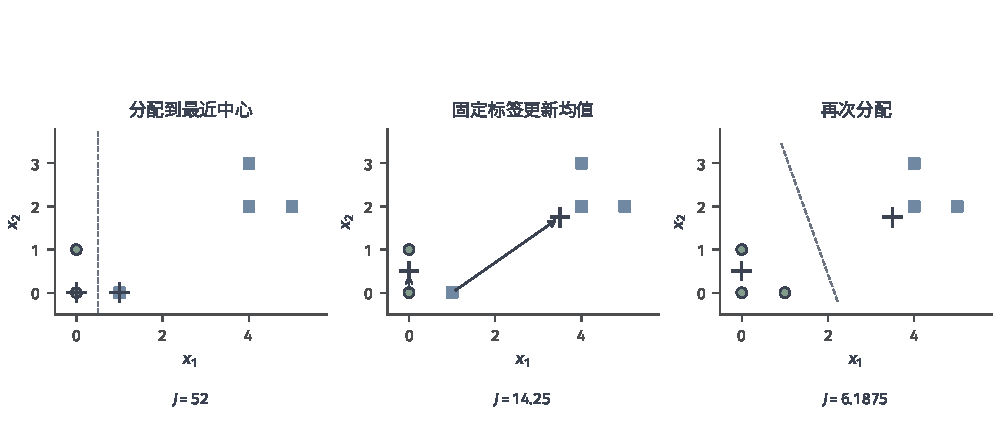
\includegraphics[width=159.059mm]{figures/03-models/01-classic-models/matplotlib/clustering-lloyd-steps/figure.pdf}
  \caption{Lloyd 迭代的教学例，六个样本为 $(0,0)$、$(0,1)$、$(1,0)$、$(4,2)$、$(4,3)$、$(5,2)$，初始中心为 $(0,0)$ 和 $(1,0)$。圆点与方块表示两个簇，十字表示中心，虚线表示等距边界。首次更新后中心为 $(0,0.5)$ 和 $(3.5,1.75)$；图中依次展示分配、均值更新与再次分配。}
 \label{fig:clustering-lloyd-steps}
\end{figure*}

平局与空簇需要纳入更新规则。等距时优先保留仍属最优的原分配，初始化则按固定顺序决定；空簇没有均值，下面保留其旧中心。这一教学实现最多返回$K$个非空簇。要求恰好$K$个非空簇时，可采用重启或后文的容量约束，并核对相应的停止条件。

\begin{codeblock}[language=Python,label={code:clustering-kmeans}]{带平局与空簇处理的 Lloyd 迭代}
import numpy as np

def kmeans(X, K, max_iter=300, seed=0):
    X = np.asarray(X, dtype=float)
    n = len(X)
    if not 1 <= K <= n or max_iter < 1:
        raise ValueError("invalid K or max_iter")
    rng = np.random.default_rng(seed)
    mu = X[rng.choice(n, K, replace=False)].copy()
    labels = np.full(n, -1)
    for _ in range(max_iter):
        d2 = ((X[:, None] - mu[None]) ** 2).sum(2)
        new = d2.argmin(1)
        rows = np.flatnonzero(labels >= 0)
        keep = d2[rows, labels[rows]] == d2[rows, new[rows]]
        new[rows[keep]] = labels[rows[keep]]
        if np.array_equal(new, labels):
            return labels, mu
        labels = new
        for k in range(K):
            members = X[labels == k]
            if len(members):
                mu[k] = members.mean(0)
    return labels, mu
\end{codeblock}

代码接受有限的二维数值数组。正常停止时，分配与中心形成不动点；迭代上限提前触发时，返回中心已按当前分配更新，但这些分配可能还需再比较一次最近中心。两种退出情形应分别记录。广播计算临时占用$O(nKd)$空间，样本较多时可分块计算距离。

初始中心决定Lloyd从哪里开始搜索。\term{K-means++}先均匀选一个样本，再按$D_i^2/\sum_jD_j^2$抽取后续中心，其中$D_i$是样本到已有中心的最近距离。所有$D_i=0$时，已有中心已覆盖全部不同位置。Arthur与Vassilvitskii证明了初始目标的期望界$\mathbb{E}[J]\leq8(\log K+2)J^\ast$；Lloyd后续不增目标，因此保留这一界\scite{clust-arthur2007}。

该界平均了初始化随机性，单次运行的结果仍可能相差较大。标准K-means++逐个选中心，约需$O(nKd)$运算；分布式实现还需计入数据扫描与通信。评价初始化时，可以同时比较最终平方误差、重启次数和总成本。

\subsubsection{理论分析}

\paragraph{表达能力}
K-means以最近中心的Voronoi区域表示分组，适合按平方距离集中在中心附近的簇。弯曲、尺度差异很大或由其他相异度定义的簇可能不在这个表示偏好内。

\paragraph{收敛性}
Lloyd的有限停止需要目标下降与平局规则共同支持。目标有下界且不增，足以得到目标值的极限；进一步排除无穷次分配变化，才可得到有限轮停止。下面利用有限分配集合完成这一步。

\begin{theorem}[Lloyd 算法的单调性与有限停止]
  \label{thm:clustering-lloyd}
  对有限样本，在精确计算下，分配步采用最近中心规则，并在平局时优先保留原簇分配；更新步对非空簇取均值、对空簇保留旧中心。则目标值单调不增，算法在有限轮后到达分配和中心均不再变化的不动点。
\end{theorem}
\begin{proof}
固定中心，逐点选择最小距离给出
\[
 J(\mathcal{P}^{(t+1)},\bm{\mu}^{(t)})
 \leq J(\mathcal{P}^{(t)},\bm{\mu}^{(t)}).
\]
对任意非空簇 $C$，记均值为 $\bar{\bm{x}}_C$。展开平方项，并利用 $\sum_{i\in C}(\bm{x}_i-\bar{\bm{x}}_C)=\bm{0}$，得到
\begin{equation}
 \sum_{i\in C}\lVert\bm{x}_i-\bm{a}\rVert_2^2
 =\sum_{i\in C}\lVert\bm{x}_i-\bar{\bm{x}}_C\rVert_2^2
   +|C|\lVert\bm{a}-\bar{\bm{x}}_C\rVert_2^2.
 \label{eq:clustering-mean-decomposition}
\end{equation}
所以均值是唯一最优中心，更新步也不会增加目标；空簇对目标贡献为零。

第一次均值更新后，若分配改变，至少一个样本移向严格更近的中心，否则保留原标签的规则会阻止改变。因此完整一轮使目标严格下降。对任一分配，均值更新后的目标只由该分配决定，即使存在空簇也如此。分配至多有 $K^n$ 种，严格下降不可能无限次访问它们。分配不变时，已有非空簇中心仍为相同均值，算法遂停止。
\end{proof}

不动点在固定中心时满足最近分配，在固定分配时满足均值最优。若每个样本的最近中心唯一、各簇非空，则足够小的中心扰动保持分配，均值最优性给出局部最优解释。等距样本或重合中心可能破坏这一局部稳定条件，需按退化结构分析。

两个子问题易解，联合的全局搜索仍可能昂贵。维数属于输入时，固定$K=2$的欧氏平方和聚类已是NP-hard\scite{clust-aloise2009}。平面上将$K$作为输入也有NP-hard结果\scite{clust-mahajan2012}。这些结果表明，在$\mathrm{P}\ne\mathrm{NP}$的前提下，一般输入的精确全局解无法统一用多项式时间取得。

\paragraph{泛化性}
未来样本$\bm{X}$与训练样本同分布时，可用总体量化误差$\mathbb{E}[\min_k\lVert\bm{X}-\bm{\mu}_k\rVert_2^2]$评价所学中心。经验全局最优中心在矩条件和适当唯一性条件下具有一致性理论\scite{clust-pollard1981}。一次Lloyd运行得到的是某个不动点，应用该理论还需核对其与经验全局解的关系。

输入表示同样影响量化误差。平方距离放大远离中心的样本，不同量纲改变最近中心的次序，因此尺度选择需对应业务含义。第\ref{sec:regression-knn}节的$k$-NN回归也依赖距离，但它平均带响应的邻居，K-means则拟合无标签输入的位置。重启改变搜索起点；修改相似度或模型改变所表达的结构，二者处理不同来源的误差。

\subsubsection{支持大规模数据（Mini-Batch K-means）}

样本量较大时，一轮全量扫描也可能超过更新预算。Sculley在2010年提出\term{小批量K均值聚类}（Mini-Batch K-means），每轮抽取$b$个样本，只调整它们涉及的中心\scite{clust-sculley2010}。

设簇 $k$ 累计接收了 $v_k$ 次样本更新。每接收一个分配到该簇的样本，就令 $v_k\leftarrow v_k+1$，并计算
\begin{equation}
 \bm{\mu}_k\leftarrow
 (1-\eta_k)\bm{\mu}_k+\eta_k\bm{x}_i,
 \qquad \eta_k=\frac{1}{v_k}.
 \label{eq:clustering-minibatch}
\end{equation}
这是对历史已分配样本的增量平均，不是当前全体簇成员的精确均值。一轮距离计算降为 $O(bKd)$，但总成本仍取决于迭代次数、初始化和最终全量分配。

随机小批量使每次更新只反映部分样本，逐轮全量SSE可能波动。批量大小、采样偏差和低频簇的覆盖影响最终误差；定理~\ref{thm:clustering-lloyd}针对完整分配与精确均值更新，其单调性前提在这里发生改变。选择计算预算时，应以抽样评价或留出量化误差检查这种近似是否足够。

\subsubsection{支持限制簇大小（Constrained K-means）}
\label{sec:clustering-capacity}

最小 SSE 不一定满足容量需求。客户分区、任务分片或服务网点分配常要求每簇至少或至多容纳一定数量的样本。Bradley、Bennett 与 Demiriz 研究了带最小簇规模的 K-means；加入上界后，固定中心的分配问题可统一写为\scite{clust-bradley2000}。
\begin{equation}
 \begin{aligned}
 \min_{\bm{Z}}\quad&
   \sum_{i=1}^n\sum_{k=1}^K
   z_{i,k}\lVert\bm{x}_i-\bm{\mu}_k\rVert_2^2,\\
 \text{s.t.}\quad&
   \sum_{k=1}^K z_{i,k}=1,\quad z_{i,k}\in\{0,1\},\\
 & \ell_k\leq\sum_{i=1}^n z_{i,k}\leq u_k.
 \end{aligned}
 \label{eq:clustering-capacity}
\end{equation}
整数容量满足 $0\leq\ell_k\leq u_k$，且在没有其他分配禁令时，可行性条件为 $\sum_k\ell_k\leq n\leq\sum_ku_k$。

固定中心的容量分配可转为最小费用流。源点到每个样本的边容量为1，样本到每簇的边容量为1、费用为平方距离，簇到汇点的边下界为$\ell_k$、上界为$u_k$，总流量为$n$。网络流的整数性保证存在整数最优解，使每个样本恰好选择一簇；这一性质来自网络约束的结构。

容量方法的中心仍按均值更新。每次分配精确最优且平局保留已有最优分配时，分配变化导致严格下降；采用确定的空簇处理后，可按有限分配集合证明停止。求解成本取决于网络规模、费用表示与求解器，需按具体实现估计。

Malinen 与 Fränti 在 2014 年研究了要求簇规模相等的平衡 K-means\scite{clust-malinen2014}。当 $K$ 整除 $n$ 且要求 $|C_k|=n/K$ 时，把每个中心复制成相应数量的容量槽，得到 $n$ 对 $n$ 的指派问题；Hungarian 算法可在 $O(n^3)$ 时间内求解。

当$n$不能被$K$整除，可为各簇指定$\lfloor n/K\rfloor$或$\lceil n/K\rceil$个槽，并使容量总和为$n$。按距离顺序填槽可以节省搜索，却可能让先处理的样本占用后续样本所需位置。使用这种启发式时，还需检查全部下界与实际SSE变化。

\subsubsection{小结}

K-means将数值硬划分写成平方失真最小化，计算便利来自最近中心与均值两个可解子问题。尺度、离群点、初始化和$K$决定实际划分；Mini-Batch减少每次更新的数据量，容量约束限制可行分配。两种扩展改变计算或约束，中心几何仍沿用原模型。

\subsection{K-medoids}
\label{sec:clustering-kmedoids}

解释客户群组时，可能希望给出一条真实记录；对字符串等对象，均值也缺乏定义。\term{K 中心样本聚类}（K-medoids）从观测对象中选代表，只依赖样本之间的相异度，因而可在这些场景中使用。

Kaufman与Rousseeuw在1987年介绍了通过medoid聚类的方法，以真实观测作代表，使相异度矩阵能够直接作为输入\scite{clust-kaufman1987}。1990年的专著进一步整理了PAM、面向较大数据的CLARA及层次分析\scite{clust-kaufman1990}。代表的解释与候选代表的搜索由此成为两个独立的设计问题。

\subsubsection{模型结构}

设代表索引集合 $M=\{m_1,\ldots,m_K\}\subseteq\{1,\ldots,n\}$，相异度为 $\delta(\bm{x},\bm{y})$。优化目标为
\begin{equation}
 J(M)=\sum_{i=1}^n\min_{m\in M}\delta(\bm{x}_i,\bm{x}_m).
 \label{eq:clustering-medoids}
\end{equation}
每个 $\bm{x}_{m_k}$ 称为\term{中心样本}（medoid），分配由最近代表决定。典型相异度包括欧氏距离、曼哈顿距离、汉明距离、编辑距离和 Jaccard 距离。目标本身不要求三角不等式，但某些索引加速方法需要这一性质。

未平方距离随远点的偏移增长较慢，真实样本约束也改变了中心的可移动范围，两者可减弱极端值对SSE均值的影响。具体鲁棒性仍由相异度和污染位置决定：离群点若改变候选代表的相对距离，也可能改变medoid。

图~\ref{fig:clustering-medoid-robustness}固定一维单簇，将最右样本由5移到12。平方距离的最优中心随均值右移，绝对距离的最优中心样本仍为中间观测2。该对照同时改变损失与代表约束，结论限于这组设定；它提供了检查极端值影响的可核算例子。

\Needspace{75mm}
\begin{figure}[htbp]
  \centering
  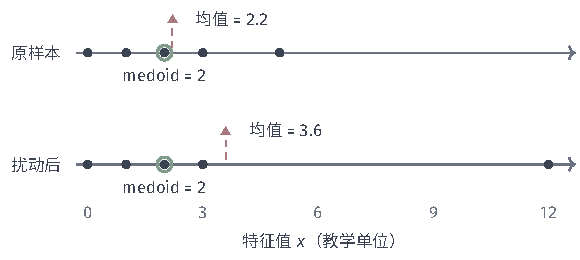
\includegraphics[width=98.231mm]{figures/03-models/01-classic-models/tikz/clustering-medoid-robustness/figure.pdf}
  \caption{中心样本与均值对极端值的不同反应。固定 $K=1$，上方样本为 $\{0,1,2,3,5\}$，下方只把 5 改为 12；黑点为观测，圆圈标出绝对距离下的 medoid，三角形标出平方距离下的最优均值。}
 \label{fig:clustering-medoid-robustness}
\end{figure}

\subsubsection{参数学习}

\term{围绕中心样本划分}（Partitioning Around Medoids, PAM）通常包含 BUILD 初始化和 SWAP 改进。BUILD 贪心增加代表；SWAP 枚举每个当前代表 $m\in M$ 与每个非代表 $o\notin M$，计算
\[
 \Delta(m,o)=
 J\bigl((M\setminus\{m\})\cup\{o\}\bigr)-J(M).
\]
候选 $o$ 来自整个数据集，而不限于 $m$ 所在簇；每次交换后，所有样本都重新选择最近代表。只在固定簇内选取距离总和最小的样本，是另一种交替更新，不能替代 PAM 的 SWAP。

下面从随机代表开始，逐个评价完整交换邻域，以便核对$J(M)$与返回状态。代码省略BUILD初始化和距离差分缓存，适合作为目标及停止判据的教学实现。

\begin{codeblock}[language=Python,label={code:clustering-pam}]{PAM 的完整交换步骤}
import numpy as np

def pam_swap(D, K, seed=0, max_iter=100):
    n = len(D)
    if D.shape != (n, n) or not 1 <= K <= n or max_iter < 1:
        raise ValueError("invalid distance matrix, K, or max_iter")
    rng = np.random.default_rng(seed)
    medoids = rng.choice(n, K, replace=False)
    cost = D[:, medoids].min(1).sum()
    converged = False
    for _ in range(max_iter):
        best, best_cost = None, cost
        outside = np.setdiff1d(np.arange(n), medoids)
        for k in range(K):
            for o in outside:
                trial = medoids.copy()
                trial[k] = o
                value = D[:, trial].min(1).sum()
                if value < best_cost:
                    best, best_cost = trial, value
        if best is None:
            converged = True
            break
        medoids, cost = best, best_cost
    return D[:, medoids].argmin(1), medoids, converged
\end{codeblock}

完整扫描若未发现改进交换，代码返回\code{converged=True}，表明当前代表集合在单次交换邻域中局部最优。迭代上限先触发时，\code{converged=False}保留了尚未核完下一邻域的状态。严格下降使代表集合不重复，去掉上限并继续扫描时，有限候选集合保证最终停止。

预计算相异度矩阵占用$O(n^2)$存储，距离本身的计算还需另外计入。经典PAM缓存最近与次近代表，一轮完整交换通常按$O(K(n-K)^2)$量级分析。教学代码为每个候选重算$K$个距离列，额外重复了这些访问，因此成本更高。

完整交换邻域昂贵时，CLARA在若干子样本上运行PAM，再用全体样本评价候选代表，以减少工作集和内存；小簇可能因抽样而遗漏。CLARANS把代表集合视为状态，随机抽取交换邻居，减少每轮扫描量\scite{clust-nghan1994}。两者分别近似候选来源与搜索邻域。

FastPAM复用不同被替换代表之间的计算，消除经典交换步骤中重复的$K$项工作，主要获得约$K$因子的加速\scite{clust-schubert2019}。关于$n$的距离访问和全量矩阵存储仍需计入，大样本的瓶颈可能继续来自这两部分。

\subsubsection{小结}

K-medoids以真实代表和一般相异度扩展原型聚类的输入与解释方式。与平方距离K-means比较时，极端值影响需结合所选损失；完整交换搜索和距离矩阵则带来额外计算。CLARA、CLARANS和FastPAM改变不同操作，可按允许的近似误差及内存预算选择。

\subsection{模型对比与总结}

原型方法可分别改变代表约束、损失、输出或表示。K-means的代表在向量空间中移动，目标是平方欧氏距离；K-medoids从观测中选代表，目标采用指定相异度。表~\ref{tab:clustering-partition}按这两个差异比较计算和用途，再讨论各方向的扩展。

\begin{table}[htbp]
 \small
 \begin{tabularx}{\linewidth}{@{}l>{\RaggedRight\arraybackslash}X>{\RaggedRight\arraybackslash}X@{}}
 \toprule
 比较项 & K-means & K-medoids\\
 \midrule
 代表 & 簇内均值向量 & 真实样本\\
 准则 & 平方欧氏距离和 & 指定相异度和\\
 优化步骤 & 最近中心与均值更新 & 代表交换与全局重分配\\
 主要成本 & 一轮 $O(nKd)$ & 完整交换搜索与距离访问\\
 典型用途 & 数值数据、向量量化 & 非数值对象、实例解释\\
 \bottomrule
 \end{tabularx}
 \caption{两类划分方法的比较。复杂度须与具体算法相联系；PAM 的成本不能套到所有 K-medoids 求解器。}
 \label{tab:clustering-partition}
\end{table}

沿中心与相异度两个方向，可以得到其他划分模型。\term{K 中位数聚类}（K-medians）最小化 $\ell_1$ 距离和，固定分配后逐坐标取中位数；它不等于以欧氏距离和定义的几何中位数问题。

\Needspace{45mm}
若簇之间允许模糊重叠，\term{模糊 C 均值}（Fuzzy C-Means, FCM）用隶属度 $u_{i,k}$ 代替硬簇分配\scite{clust-bezdek1981}。
\begin{equation}
 J_{\mathrm{FCM}}
 =\sum_{i=1}^n\sum_{k=1}^K
 u_{i,k}^{q}\lVert\bm{x}_i-\bm{\mu}_k\rVert_2^2,
 \quad \sum_k u_{i,k}=1,\quad q>1.
 \label{eq:clustering-fcm}
\end{equation}
这里$q$控制隶属度的模糊程度。固定隶属度时，中心是以 $u_{i,k}^q$ 为权重的均值；当各距离非零时，固定中心给出
\[
 u_{i,k}=
 \left[
 \sum_{j=1}^K
 \left(\frac{\lVert\bm{x}_i-\bm{\mu}_k\rVert_2}
 {\lVert\bm{x}_i-\bm{\mu}_j\rVert_2}\right)^{2/(q-1)}
 \right]^{-1}.
\]
若样本与一个或多个中心重合，可把隶属度集中在这些零距离中心上。隶属度表示模糊目标下的软归属；赋予生成后验含义还需要相应概率模型。医学影像中一个像素混合多种组织的部分体积效应，可为这种软表达提供应用动机。

\term{二分 K-means}（Bisecting K-means）改变分裂顺序：先把全部样本放在一簇，再反复选择一个簇作$K=2$划分。常见实现选择最大SSE的簇，并为每次二分多次重启。它形成层次结构，早期分裂限制后续分组，因此最终SSE应与同条件的一次性$K$分比较。Steinbach等在文档聚类中研究了这一方案\scite{clust-steinbach2000}。

% 将核距离推导及两条较长的引文安排在同一段版面内。
\Needspace{105mm}
若主要困难是原空间中的非凸形状，可在特征映射 $\phi$ 后运行\term{核 K-means}（kernel K-means）。使用第\ref{sec:classic-overview-kernel-trick}节定义的正定核$K$，本节只需把簇内平方距离改为特征空间距离。样本到簇均值的平方距离为
\begin{equation}
 \begin{aligned}
 \lVert\phi(\bm{x}_i)-\bm{\mu}_k^\phi\rVert^2
 ={}&K(\bm{x}_i,\bm{x}_i)
 -\frac{2}{|C_k|}\sum_{j\in C_k}K(\bm{x}_i,\bm{x}_j)\\
 &+\frac{1}{|C_k|^2}
   \sum_{j,l\in C_k}K(\bm{x}_j,\bm{x}_l).
 \end{aligned}
 \label{eq:clustering-kernel-kmeans}
\end{equation}
公式只使用核值，省去了显式构造$\phi$，相应成本转为核矩阵计算与存储\scite{clust-girolami2002,dhillon2004}。Girolami讨论核空间聚类，Dhillon、Guan与Kulis进一步联系了适当权重和核构造下的核K-means与归一化割。

核K-means与归一化割的联系依赖适当的权重和核构造，适用范围需随具体等价关系核对。特征映射可以改变原空间的分配形状，层次结构则改变输出粒度。第\ref{sec:clustering-hierarchy}节再讨论多层输出，下面先利用局部密度和连接描述弯曲群组。

\section{基于邻域的聚类}
\label{sec:clustering-density}

环形、月牙形和弯曲条带中的样本可能远离同一中心，却能沿密集区域连接。密度方法据此把低密度分隔加入簇定义：一类方法寻找密集区域的连通分量，另一类寻找密度峰的吸引域。同一连通区域可以包含多个峰，因此两种定义会产生不同划分。

DBSCAN 直接用邻域计数判断密集程度，OPTICS 保留不同密度尺度的访问结构，Mean Shift 则沿核密度估计寻找驻点。噪声识别是前两者的显式输出；基本 Mean Shift 会为起点寻找归宿，并不自动拒绝孤立样本。

\subsection{DBSCAN}
\label{sec:clustering-dbscan}

DBSCAN（Density-Based Spatial Clustering of Applications with Noise）用“周围是否有足够多邻居”判断一个样本能否继续扩展簇。Ester 等在 1996 年提出这一方法，使任意形状的密集连通区域和噪声能够在同一流程中处理\scite{ester1996}。

原始DBSCAN面向带噪声的大型空间数据库，将任意形状的密集区域、参数知识需求和处理成本列为设计问题。邻域计数决定哪些点能扩展，连通搜索把它们组织成簇，无法归属的点保留噪声标记。这样，簇的数量和拒绝范围由局部密度关系共同确定。

\subsubsection{模型结构}

固定半径 $\varepsilon>0$ 和最小邻域样本数 $m=\mathrm{MinPts}$，定义索引邻域
\[
 N_\varepsilon(i)=
 \{j:\delta(\bm{x}_i,\bm{x}_j)\leq\varepsilon\}.
\]
本节假定相异度对称、样本到自身距离为零，并在邻域计数中包含自身。\term{核心点}（core point）满足 $|N_\varepsilon(i)|\geq m$；\term{边界点}（border point）不是核心点，但处在某个核心点的邻域内；既非核心也非边界的样本是\term{噪声点}（noise point）。

若 $i$ 是核心点且 $j\in N_\varepsilon(i)$，称 $j$ 从 $i$\term{直接密度可达}（directly density-reachable）。沿这样的有向关系组成有限链，就得到\term{密度可达}（density-reachable）：链上除终点外的点都须为核心点，终点可以是边界点。若存在一个核心点，使两个样本都从它密度可达，则称它们\term{密度相连}（density-connected）。

先只看核心点邻接图，可以清楚地区分扩展与吸收：距离不超过$\varepsilon$的核心点相连，每个连通分量提供一个簇的核心，再吸收相邻非核心点。边界点可能同时邻接多个分量；实际DBSCAN通常交给先访问它的簇，从而得到单一标签。图~\ref{fig:clustering-dbscan}展示了核心点继续扩展、边界点只被吸收的差别。

\begin{figure}[htbp]
  \centering
  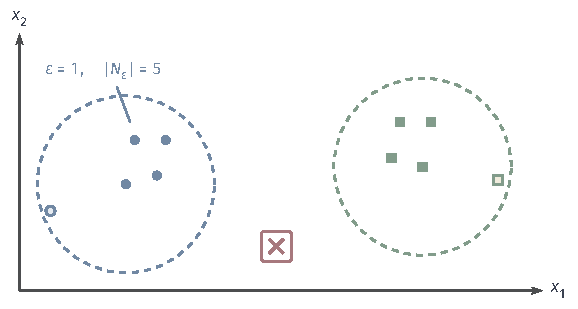
\includegraphics[width=97.850mm]{figures/03-models/01-classic-models/tikz/clustering-dbscan/figure.pdf}
  \caption{DBSCAN的教学示意，取$\varepsilon=1$、$\mathrm{MinPts}=4$，计数包含自身。圆形和方形分别标识两个核心分量，颜色只作辅助；实心标记为核心点，浅色填充标记为边界点，红框叉号为噪声。虚线圆表示两个示例核心点的邻域；左侧标注直接给出邻域内计数，边界点不能继续扩展簇。}
 \label{fig:clustering-dbscan}
\end{figure}

\subsubsection{参数学习}

DBSCAN 的主要工作是查询邻域并搜索核心连通分量。代码~\ref{code:clustering-dbscan} 使用暴力距离查询，完整展示暂定噪声被重新吸收为边界点的情况。

\begin{codeblock}[language=Python,label={code:clustering-dbscan}]{DBSCAN 的邻域扩展}
import numpy as np
from collections import deque

def dbscan(X, eps, min_pts):
    X = np.asarray(X, dtype=float)
    if eps <= 0 or min_pts < 1:
        raise ValueError("invalid density parameters")
    labels = np.full(len(X), -1)  # -1 未访问，-2 噪声
    def neighbors(i):
        d2 = ((X - X[i]) ** 2).sum(1)
        return np.flatnonzero(d2 <= eps ** 2)
    cid = 0
    for i in range(len(X)):
        if labels[i] != -1:
            continue
        near = neighbors(i)
        if len(near) < min_pts:
            labels[i] = -2
            continue
        labels[i] = cid
        queue = deque(near)
        while queue:
            j = queue.popleft()
            if labels[j] == -2:
                labels[j] = cid
            if labels[j] != -1:
                continue
            labels[j] = cid
            near_j = neighbors(j)
            if len(near_j) >= min_pts:
                queue.extend(near_j)
        cid += 1
    return labels
\end{codeblock}

代码中每个样本至多查询一次邻域，队列则可能保存重复索引。暴力距离计算约需$O(n^2d)$运算。低维数据且邻域规模受控时，空间索引可使实践成本接近$O(n\log n)$；高维或大半径会增加访问量，最坏仍可达到平方级。预存全部邻域还可能占用$O(n^2)$内存。

参数选择可从第 $m$ 近邻距离的排序图入手，近邻计数约定应与是否包含自身一致。曲线的转折提示不同密度尺度，但未必存在清晰肘部。Schubert 等把 $\mathrm{MinPts}\approx 2d$ 作为平滑密度估计的经验起点，而不是一般最优值\scite{clust-schubert2017}。重复样本、噪声比例和有效维数都会影响合理的邻域大小与最小样本数。

\subsubsection{理论分析}

\paragraph{表达能力}
DBSCAN以核心点连通区域表达密度簇，可以保留非凸形状。一个共同邻域半径和阈值却未必能同时适应相差很大的密度，细桥或邻域尺度失配也会改变分组。

\paragraph{收敛性}
DBSCAN的访问和扩展在有限样本上结束，其计算任务是搜索核心连通分量。由于这里没有连续参数的迭代优化，需要验证的是搜索是否完整，以及固定数据下哪些输出与访问顺序无关。

\begin{theorem}[DBSCAN 的核心点确定性]
 \label{thm:clustering-dbscan}
 固定数据、对称相异度和参数 $(\varepsilon,m)$，DBSCAN 输出的每个簇限制到核心点后，恰为核心点邻接图的一个连通分量。因此核心点划分与访问顺序无关，簇编号的置换除外。
\end{theorem}
\begin{proof}
在核心点集合上，距离不超过 $\varepsilon$ 的两点能相互直接密度到达。有限链的连通关系满足自反、对称和传递性，故图的连通分量就是核心点上密度相连关系的等价类。

从任一尚未访问的核心点扩展时，每发现一个核心邻居就加入它的邻域。沿路径长度归纳，该点所在连通分量中的每个核心点最终都会被访问。反过来，扩展过程只能经由核心点邻接边到达其他核心点，不能穿过非核心边界点连接两个分量。因此输出的核心集合既不遗漏本分量，也不包含其他分量，结论成立。
\end{proof}

定理固定了核心点划分。一个边界点若邻接多个核心分量，其单一归属仍由访问规则决定；簇编号和共享边界归属是两种不同的顺序影响。

\paragraph{泛化性}
重新运行时，新增样本会改变邻域计数：原边界点可能达到核心阈值，新核心点也可能连接两个分量。因此，定理对固定数据的确定性与抽样扰动下的稳定性属于不同问题。

DBSCAN通常为当前样本给出分组。预测新样本时，可依据已有核心点的邻接关系定义分配，并规定多簇冲突和拒绝；将新样本纳入数据重新搜索则可能改变原分量。密度差异较大时，小$\varepsilon$可能拆开稀疏群组，大$\varepsilon$可能连上邻近稠密群组，尺度选择需同时检查这些影响。

\subsubsection{小结}

DBSCAN由局部计数产生核心点，再以连通性形成簇，并显式保留噪声。它省去预设$K$，同时引入全局半径、计数阈值及距离选择。可恢复的形状由密度连通定义决定，高维查询和不同密度群组仍可能限制实际效果。

\subsection{OPTICS}
\label{sec:clustering-optics}

反复调整 DBSCAN 的半径会重复查询相似邻域。OPTICS（Ordering Points To Identify the Clustering Structure）保留一次搜索中的密度排序，使分析者能够事后读取不同尺度的结构。Ankerst 等在 1999 年提出的方法输出排序与距离记录，而非直接输出唯一划分\scite{clust-ankerst1999}。

OPTICS把邻域计算与划分提取分开。DBSCAN在给定尺度后返回簇标签，OPTICS先保存访问次序和距离，供后续比较多种尺度。探索密度群组因而主要转为读取同一份结果，同时需要明确采用的提取规则。

\subsubsection{模型结构}

设搜索半径上限为 $\varepsilon_{\max}$。若样本 $i$ 在该半径内有至少 $m$ 个邻居，则其\term{核心距离}（core distance）为第 $m$ 近邻距离；否则记为 $+\infty$：
\[
 a_i=
 \begin{cases}
 \delta_{i,(m)},&|N_{\varepsilon_{\max}}(i)|\geq m,\\
 +\infty,&\text{其他情况}.
 \end{cases}
\]
由核心点 $i$ 到邻居 $j$ 的\term{可达距离}（reachability distance）定义为
\begin{equation}
 r(j\mid i)=\max\{a_i,\delta(\bm{x}_i,\bm{x}_j)\}.
 \label{eq:clustering-reachability}
\end{equation}
方向来自出发点的核心距离，因此通常 $r(j\mid i)\ne r(i\mid j)$。它表示在确保出发点足够密集的同时覆盖 $j$ 所需的半径。

OPTICS 为每个样本记录访问次序、核心距离和当前获得的最小可达距离。按访问次序画出可达距离形成\term{可达图}（reachability plot）；低谷通常对应容易从内部到达的密集区域，较高的过渡位置提示区域之间的分隔。

\subsubsection{参数学习}

从一个未处理点开始，算法输出该点并查询邻域。如果它是核心点，就用式~\eqref{eq:clustering-reachability} 更新未处理邻居的最小可达距离；优先队列每次取出当前可达距离最小的点，继续同样的过程。队列为空而仍有未处理点时，再开始一个新的搜索。这个过程是按可达距离优先的遍历，而不是普通先进先出的广度优先搜索。

给定 $\varepsilon'\leq\varepsilon_{\max}$，提取 DBSCAN 式结构时必须同时使用核心距离。沿排序扫描，若某点的记录可达距离大于 $\varepsilon'$，但核心距离不大于 $\varepsilon'$，它应开启一个新簇；若二者都大于阈值，才暂记为噪声；可达距离不大于阈值的点接续当前簇。只把水平线下的连续段当作簇，会漏掉可达距离很大、却负责开启新簇的核心点。不同提取规则对部分边界点的处理还可能与重新运行 DBSCAN 不同。

图~\ref{fig:clustering-optics-reachability} 将原始样本间距与可达图对应起来。中间一组样本较稀疏，形成的谷底较高；用 $\varepsilon'=0.35$ 提取时它们不构成核心簇，增大阈值才会纳入。次序 1、8、14 对应三次重新开始的搜索，其可达距离为无穷；次序 23 的孤立点也有无穷可达距离，但它的核心距离同样无穷，因而不能开启簇。

\begin{figure}[htbp]
  \centering
  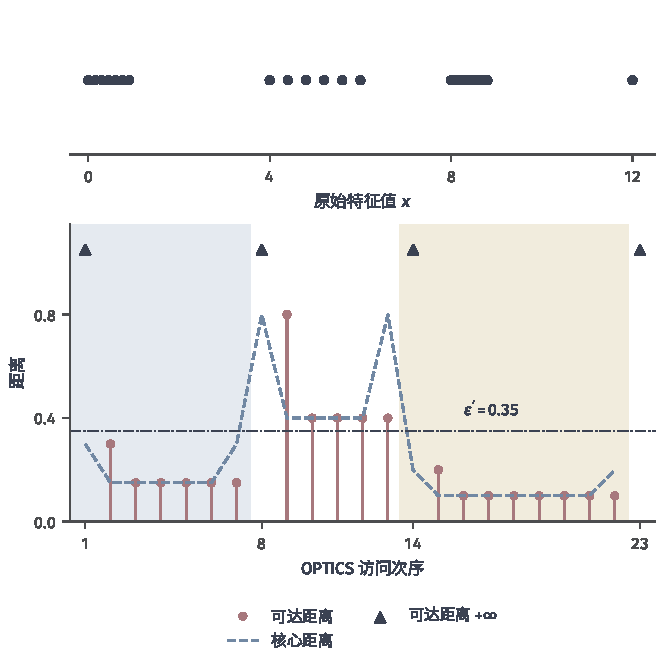
\includegraphics[width=105.412mm]{figures/03-models/01-classic-models/matplotlib/clustering-optics-reachability/figure.pdf}
  \caption{固定一维教学数据上的OPTICS排序，取$\mathrm{MinPts}=3$（含自身）、$\varepsilon_{\max}=1.1$。三组样本的间距分别为$0.15$、$0.4$、$0.1$，另有$x=12$的孤立点。红色竖棒为可达距离，蓝色虚线为核心距离；蓝、黄底色标出两个低谷。无穷可达距离用顶部三角形表示，不能按其显示高度作数值比较；水平点划线展示阈值切割在本例中提取哪些低谷。}
 \label{fig:clustering-optics-reachability}
\end{figure}

低谷也可按相对陡降、陡升的$\xi$规则提取，并结合最小簇规模、前驱关系及嵌套处理。原始OPTICS已讨论陡峭区域，后续工作进一步构造密度层次。这里的自动提取减少人工读图，尺度和粒度仍由提取参数控制。

\subsubsection{小结}

OPTICS保留一次搜索中的多尺度结构，便于比较不同密度群组；结果受$\varepsilon_{\max}$、$\mathrm{MinPts}$和提取规则共同影响。空间索引与邻域规模有利时可减少搜索，最坏成本仍可能为平方级。优先队列和距离记录增加了操作与存储，应按同一数据和目标粒度与DBSCAN比较。

\subsection{Mean Shift}
\label{sec:clustering-mean-shift}

密度连通方法检查样本之间是否存在密集路径；\term{均值漂移}（Mean Shift）则在估计密度上搜索模态。它反复计算当前位置附近的加权均值并移动搜索点，先得到估计密度的驻点，再据起点的归宿形成分组。

% 两段历史含三条较长引文，同时为边栏预留空间。
\Needspace{125mm}
Fukunaga与Hostetler在1975年从密度梯度估计出发，将局部均值偏移用于模式识别\scite{clust-fukunaga1975}。搜索先回答密度增加的方向，再据轨迹确定归宿，因此无需预先给出簇边界。

Cheng在1995年推广核与权重，讨论均值漂移、模态搜索和聚类之间的联系\scite{clust-cheng1995}。Comaniciu与Meer在2002年系统分析该方法，并展示特征空间和图像分割中的应用\scite{clust-comaniciu2002}。这些工作将密度上的移动规则与随后得到的簇分配联系起来，二者仍需分别规定停止与合并方式。

\subsubsection{模型结构}

以径向核估计未知密度。设 $h>0$ 为带宽，核函数为 $\mathcal{K}(\bm{u})=c_k k(\lVert\bm{u}\rVert_2^2)$，其中$c_k$是归一化常数，$k$是剖面函数（profile），规定核权重怎样随距离平方变化。则\term{核密度估计}（kernel density estimation, KDE）为
\begin{equation}
 \hat f(\bm{y})=\frac{c_k}{nh^d}
 \sum_{i=1}^n
 k\left(\frac{\lVert\bm{y}-\bm{x}_i\rVert_2^2}{h^2}\right).
 \label{eq:clustering-kde}
\end{equation}
可以从各样本出发在估计密度上搜索，把趋向同一模态的起点归为一簇。带宽决定平滑尺度，小带宽通常保留细节，大带宽通常合并邻近结构；模态数量的具体变化还依赖维数、核与样本分布。

\subsubsection{参数学习}

令 $g(u)=-k'(u)$，并记 $u_i(\bm{y})=\lVert\bm{y}-\bm{x}_i\rVert_2^2/h^2$。直接对式~\eqref{eq:clustering-kde} 求导可得
\[
 \nabla\hat f(\bm{y})=
 \frac{2c_k}{nh^{d+2}}
 \sum_i g(u_i(\bm{y}))(\bm{x}_i-\bm{y}).
\]
只要权重和为正，梯度便是正系数乘以\term{均值漂移向量}
\[
 \bm{m}(\bm{y})=
 \frac{\sum_i g(u_i(\bm{y}))\bm{x}_i}
      {\sum_i g(u_i(\bm{y}))}-\bm{y}.
\]
因此采用下列自适应步长的梯度方向更新：
\begin{equation}
 \bm{y}^{(t+1)}=
 \frac{\sum_i w_i^{(t)}\bm{x}_i}{\sum_i w_i^{(t)}},
 \qquad w_i^{(t)}=g(u_i(\bm{y}^{(t)})).
 \label{eq:clustering-mean-shift}
\end{equation}
权重来自一元剖面函数的负导数$g$，其自变量是距离平方。高斯剖面$k(u)=\exp(-u/2)$给出与高斯权重成比例的$g$，Epanechnikov剖面$(1-u)_+$在支撑内部给出常数权重，边界按分段规则处理。

式~\eqref{eq:clustering-mean-shift}与第\ref{sec:regression-nadaraya-watson}节的Nadaraya--Watson回归都计算核加权平均。Mean Shift平均输入位置，更新搜索点；核回归平均响应，预测条件均值。相同的平均运算承担不同的估计任务。

图~\ref{fig:clustering-mean-shift-modes}固定同一组一维样本，两个起点沿式~\eqref{eq:clustering-mean-shift}分别向左右峰移动，靠近驻点时位移减小。灰线改用更大带宽，两个峰合为一个峰。起点决定从哪里搜索，带宽改变估计密度及可到达的模态，两项选择因而影响不同的对象。

\Needspace{90mm}
\begin{figure}[htbp]
  \centering
  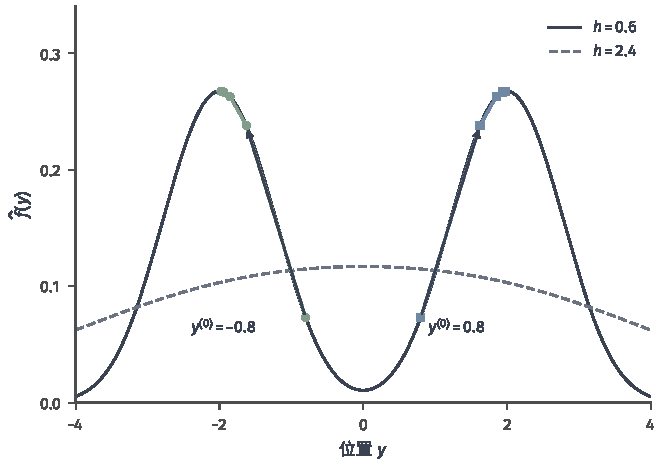
\includegraphics[width=105.412mm]{figures/03-models/01-classic-models/matplotlib/clustering-mean-shift-modes/figure.pdf}
  \caption{Mean Shift 的密度爬升与带宽效应。左右各有三个样本，位置为 $-2.5,-2,-1.5$ 和 $1.5,2,2.5$，均采用高斯核。彩色标记给出带宽 $h=0.6$ 时从 $\pm0.8$ 出发的初始位置和四次更新，箭头指示第一次移动；灰色虚线对应 $h=2.4$，轨迹在黑色实线上计算。}
 \label{fig:clustering-mean-shift-modes}
\end{figure}

\begin{codeblock}[language=Python,label={code:clustering-mean-shift}]{高斯 Mean Shift 的起点更新}
import numpy as np

def mean_shift_positions(X, h, max_iter=300, tol=1e-4):
    X = np.asarray(X, dtype=float)
    if h <= 0:
        raise ValueError("h must be positive")
    Y = X.copy()
    for _ in range(max_iter):
        d2 = ((Y[:, None] - X[None]) ** 2).sum(2)
        log_w = -d2 / (2 * h * h)
        log_w -= log_w.max(1, keepdims=True)
        W = np.exp(log_w)
        new = (W @ X) / W.sum(1, keepdims=True)
        step = np.linalg.norm(new - Y, axis=1).max()
        Y = new
        if step <= tol:
            break
    return Y
\end{codeblock}

代码返回最终位置。得到簇标签还需合并相近终点，例如构造距离不超过$\rho$的终点图并取连通分量；$\rho=h/2$可作教学起点。这个合并阈值与更新容差用途不同，连通规则可能沿一串近终点把不同模态接在一起，需单独检查。

全部$n$个起点的一轮精确更新约需$O(n^2d)$运算。高斯核覆盖所有样本，因此截断邻域或近似近邻改变了精确更新。大数据实现可分块、减少起点或改用有限支撑核，并分别核对计算节省与位置误差。

\subsubsection{理论分析}

\paragraph{表达能力}
Mean Shift以核密度的吸引域组织簇，带宽决定哪些峰被保留。多个真实群体可能被平滑成一个峰，一个群体也可能对应多个峰；密度模态不必等同于任务类别。

\paragraph{收敛性}
Mean Shift的上升不等式控制密度值，位置收敛还需排除轨迹在多个聚点之间移动。步长平方可和只说明步长趋零，后续研究指出了将它直接推为Cauchy性的缺口\scite{clust-aliyari2015}。下面用紧性、连续性和有限固定点补足这一步。

\begin{theorem}[Mean Shift 的密度单调性与条件收敛]
 \label{thm:clustering-mean-shift}
 设 $k$ 非负、凸、非增且可微，$k(0)<\infty$，迭代中权重和始终为正。则式~\eqref{eq:clustering-mean-shift} 产生的密度值单调不减且收敛。若进一步假设 $g=-k'$ 连续且严格为正，样本凸包内的固定点只有有限个，则位置序列也收敛，极限为 $\hat f$ 的驻点。
\end{theorem}
\begin{proof}
简记 $\bm{y}=\bm{y}^{(t)}$、$\bm{y}'=\bm{y}^{(t+1)}$。由凸性，
\[
 k(u_i(\bm{y}'))-k(u_i(\bm{y}))
 \geq g(u_i(\bm{y}))
       \bigl(u_i(\bm{y})-u_i(\bm{y}')\bigr).
\]
令 $w_i=g(u_i(\bm{y}))$、$s=\sum_iw_i$。由于 $\bm{y}'$ 是加权均值，展开平方后交叉项为零，得到
\[
 \sum_iw_i\bigl(
 \lVert\bm{y}-\bm{x}_i\rVert_2^2
 -\lVert\bm{y}'-\bm{x}_i\rVert_2^2\bigr)
 =s\lVert\bm{y}'-\bm{y}\rVert_2^2.
\]
所以
\begin{equation}
 \hat f(\bm{y}')-\hat f(\bm{y})
 \geq\frac{c_k s}{nh^{d+2}}
       \lVert\bm{y}'-\bm{y}\rVert_2^2\geq0.
 \label{eq:clustering-mean-shift-ascent}
\end{equation}
又有 $\hat f(\bm{y})\leq c_k k(0)/h^d$，故密度值收敛。

在附加条件下，第一次更新后所有位置均在有限样本的紧凸包内。距离平方因此有界，而连续正函数 $g$ 在相应紧区间上有正下界，故 $s$ 也有统一正下界。对式~\eqref{eq:clustering-mean-shift-ascent} 求和，得到步长平方可和，特别地，$\lVert\bm{y}^{(t+1)}-\bm{y}^{(t)}\rVert_2\to0$。

记连续更新映射为 $T$。任取收敛子列 $\bm{y}^{(t_j)}\to\bm{y}^\ast$，步长趋零与连续性给出 $T(\bm{y}^\ast)=\bm{y}^\ast$，所以每个聚点都是固定点。固定点有限，取彼此不相交的小球包围它们；序列最终必在这些小球的并集中，否则紧性会产生球外聚点。步长最终小于球之间的间隙，故序列不能再从一个球跳到另一个球。任意缩小球半径，便知它只能趋向其中一个固定点。梯度公式最后给出 $\nabla\hat f(\bm{y}^\ast)=\bm{0}$。
\end{proof}

位置收敛由紧性、连续性及有限固定点共同支持，平方可和用于先证明步长趋零。极限是驻点，特殊起点可能停在鞍点；解释为密度峰还需检查局部形状。Epanechnikov核的分段边界和零权重不满足第二部分的全部条件，需另作分析。

\paragraph{泛化性}
留出样本上的模态结构取决于带宽及密度估计误差。KDE在适当光滑性和随$n$缩小的带宽等条件下可一致估计密度；从密度误差控制到峰位置、吸引域和簇分配的稳定，还需正则条件。当前固定KDE上的上升定理只处理搜索计算。

\subsubsection{小结}

Mean Shift以局部加权均值实现密度爬升，随后按模态归宿组织簇。簇数由带宽、起点和终点合并共同决定。图像分割与跟踪可利用这种聚集机制，使用时需同时检查计算预算、驻点类型及带宽变化下的分组。

\subsection{模型对比与总结}

三种邻域方法形成不同输出：DBSCAN给固定尺度下的核心连通簇，OPTICS保存多尺度排序，Mean Shift搜索平滑密度的驻点。连通区域含多个峰时，结果可在相近尺度下不同。噪声拒绝也需逐方法检查；下面的扩展进一步把网格或层次加入密度表示。

DENCLUE叠加样本影响函数形成密度，用吸引点及其连通关系组织簇，以密度阈值标记噪声，并借网格辅助计算\scite{clust-hinneburg1998}。它与Mean Shift共享密度估计视角，估计在高维是否可靠仍取决于样本量、表示和核尺度。

HDBSCAN 把核心距离用于定义\term{互可达距离}（mutual reachability distance）：
\[
 \delta_{\mathrm{mr}}(i,j)
 =\max\{a_i,a_j,\delta(\bm{x}_i,\bm{x}_j)\}.
\]
在这一距离上构造最小生成树并形成密度层次，再按最小簇规模压缩层次、按跨尺度持续性选择簇，可以减轻单一 $\varepsilon$ 的限制。Campello 等给出了这一层次密度框架\scite{clust-campello2013}。

HDBSCAN的跨尺度持续性是层次中的簇选择量，评估抽样扰动还需要另外的统计协议。最小簇规模等参数继续控制输出，高维距离的区分度也需检验。密度路线将低密度分隔纳入簇定义；已有可信样本关系时，还可直接用图建立群组。

\section{基于图的聚类}
\label{sec:clustering-graph}

社交连接、文档相似度和像素邻接可以直接表示为加权图。图聚类将样本作为顶点、相似程度作为边权，寻找内部连接较强而外部连接较弱的群组。向量距离也可用于建图；边权和邻域规则因此继续决定所保留的相似关系。

仅最小化切边权重，可能轻易切下一个连接少的小块。对簇规模或连接体积作归一化，可以比较“割断多少联系”与“簇原来拥有多少联系”。谱聚类再把这一离散搜索松弛为特征向量求解。

\subsection{谱聚类}
\label{sec:clustering-spectral}

\term{谱聚类}（spectral clustering）先以图拉普拉斯的特征向量表示顶点，再将顶点划分为簇。第\ref{sec:dim-le}节的拉普拉斯特征映射共享建图与低频谱表示，但输出连续坐标；聚类还需要离散分配。von Luxburg的教程整理了图构造、归一化及适用条件\scite{clust-luxburg2007}。下面以归一化割及多簇谱算法展开这一流程。

Donath与Hoffman在1973年用谱信息给图划分代价建立下界，将组合搜索与可计算特征值联系起来\scite{clust-donath1973}。Shi与Malik进一步用像素相似关系建立归一化割，相关会议和期刊论文分别发表于1997年和2000年\scite{clust-shi2000}。Ng、Jordan与Weiss在2001年会议提出多簇谱嵌入与行归一化，论文集于2002年出版\scite{clust-ng2002}。这些工作分别解释了图目标、连续表示及离散化的连接。

\subsubsection{模型结构}

设无向图的非负对称权重矩阵为 $\bm{W}\in\mathbb{R}^{n\times n}$，通常令 $w_{i,i}=0$。向量样本可用高斯相似度 $\exp(-\lVert\bm{x}_i-\bm{x}_j\rVert_2^2/(2\sigma^2))$ 构造边；近邻图则保留部分局部关系。单向近邻关系未必对称，必须明确采用并集对称化还是互近邻规则。

定义顶点度 $d_i=\sum_jw_{i,j}$、度矩阵 $\bm{D}=\operatorname{diag}(d_1,\ldots,d_n)$，以及三种拉普拉斯：
\begin{align}
 \bm{L}&=\bm{D}-\bm{W},\nonumber\\
 \bm{L}_{\mathrm{sym}}
 &=\bm{I}-\bm{D}^{-1/2}\bm{W}\bm{D}^{-1/2},\nonumber\\
 \bm{L}_{\mathrm{rw}}
 &=\bm{I}-\bm{D}^{-1}\bm{W}.
 \label{eq:clustering-laplacians}
\end{align}
归一化所用逆度数要求$d_i>0$，因此先单独处理孤立顶点。$\bm{L}_{\mathrm{rw}}$ 一般不对称，但与 $\bm{L}_{\mathrm{sym}}$ 相似，因而有相同的实特征值。对任意 $\bm{v}\in\mathbb{R}^n$，
\begin{equation}
 \bm{v}^{\top}\bm{L}\bm{v}
 =\frac12\sum_{i,j}w_{i,j}(v_i-v_j)^2\geq0.
 \label{eq:clustering-laplacian-form}
\end{equation}
所以 $\bm{L}$ 半正定，且 $\bm{L}\bm{1}=\bm{0}$；零特征值的重数等于连通分量数，图连通时才为单重。

归一化还具有随机游走解释。转移矩阵 $\bm{P}=\bm{D}^{-1}\bm{W}$ 让游走者按边权比例选择下一顶点，且 $\bm{L}_{\mathrm{rw}}=\bm{I}-\bm{P}$。从一个簇出发，若内部连接强而外部连接弱，游走就倾向在簇中停留较久；Meilă 与 Shi 据此研究了聚类的随机游走视角\scite{clust-meila2001}。

设 $\operatorname{cut}(A,\bar A)=\sum_{i\in A,j\notin A}w_{i,j}$，$\operatorname{vol}(A)=\sum_{i\in A}d_i$。\term{归一化割}（normalized cut, NCut）定义为
\begin{equation}
 \operatorname{NCut}(\mathcal{P})
 =\sum_{k=1}^K
 \frac{\operatorname{cut}(C_k,\bar C_k)}
      {\operatorname{vol}(C_k)}.
 \label{eq:clustering-ncut}
\end{equation}
它比较切边与簇内外连接体积，减轻小簇的偏好；同体积的簇可以含不同样本数\scite{clust-shi2000}。\term{比率割}（RatioCut）则把分母换成 $|C_k|$，对应未归一化拉普拉斯的松弛。

\subsubsection{参数学习}

为把 NCut 改写成矩阵目标，定义 $\bm{F}\in\mathbb{R}^{n\times K}$，其中
\[
 f_{i,k}=
 \begin{cases}
  1/\sqrt{\operatorname{vol}(C_k)},&i\in C_k,\\
  0,&i\notin C_k.
 \end{cases}
\]
簇互不相交给出 $\bm{F}^{\top}\bm{D}\bm{F}=\bm{I}_K$。由式~\eqref{eq:clustering-laplacian-form}，第 $k$ 列的二次型恰为第 $k$ 项归一化割，故目标为 $\operatorname{tr}(\bm{F}^{\top}\bm{L}\bm{F})$。

困难在于每行只允许一个特定的非零值。去掉这一离散约束，令 $\bm{H}=\bm{D}^{1/2}\bm{F}$，得到
\begin{equation}
 \min_{\bm{H}^{\top}\bm{H}=\bm{I}_K}
 \operatorname{tr}(\bm{H}^{\top}
                   \bm{L}_{\mathrm{sym}}\bm{H}).
 \label{eq:clustering-spectral-relaxation}
\end{equation}
Shi--Malik 方法也可写为广义特征问题 $\bm{L}\bm{f}=\lambda\bm{D}\bm{f}$，与归一化变换相联系\scite{clust-shi2000}。取 $\bm{L}_{\mathrm{sym}}$ 最小的 $K$ 个特征值对应的特征向量，即得到式~\eqref{eq:clustering-spectral-relaxation} 的最优解，下节给出证明。

连续解还需离散化。\term{NJW 算法}把 $\bm{H}$ 每一行归一化到单位长度，再对行向量运行 K-means\scite{clust-ng2002}。若图恰有 $K$ 个连通分量，理想谱空间中每个分量对应同一方向；行归一化消除度数造成的长度差异，图~\ref{fig:clustering-spectral} 展示了这一解释。连接较弱的实际图中，这只是近似结构。

\Needspace{62mm}
\begin{figure}[htbp]
  \centering
  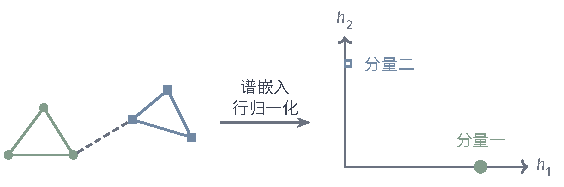
\includegraphics[width=95.564mm]{figures/03-models/01-classic-models/tikz/clustering-spectral/figure.pdf}
  \caption{谱聚类的理想情形：圆形与方形分别标识两个互不连接的分量，颜色只作辅助；在归一化谱空间中，两个分量分别落到两个方向。细虚线表示实际数据中可能存在的弱连接；加入这些连接后，谱坐标通常形成近似群组。}
 \label{fig:clustering-spectral}
\end{figure}

\begin{codeblock}[language=Python,label={code:clustering-spectral}]{给定相似度矩阵的 NJW 算法}
import numpy as np
from scipy.linalg import eigh

def spectral_clustering(W, K):
    W = np.asarray(W, dtype=float)
    n = len(W)
    if W.shape != (n, n) or not 1 <= K <= n:
        raise ValueError("invalid shape or K")
    if (W < 0).any() or not np.allclose(W, W.T):
        raise ValueError("W must be nonnegative and symmetric")
    degree = W.sum(1)
    if (degree <= 0).any():
        raise ValueError("handle isolated vertices first")
    inv = 1 / np.sqrt(degree)
    L = np.eye(n) - inv[:, None] * W * inv[None, :]
    _, H = eigh(L, subset_by_index=[0, K - 1])
    length = np.linalg.norm(H, axis=1)
    if (length == 0).any():
        raise ValueError("zero embedding row")
    labels, _ = kmeans(H / length[:, None], K)
    return labels
\end{codeblock}

代码复用代码~\ref{code:clustering-kmeans}的K-means函数，处理能放入内存的稠密矩阵。图的连通分量数超过$K$时，所选零特征子空间可能含零行，也可能将多个分量任意合并。应先确定各连通分量是否需要独立输出，再选择谱子空间与分配策略。

稠密建图约需$O(n^2d)$距离运算和$O(n^2)$存储，完整特征分解约需$O(n^3)$。只求部分特征向量时，可用Lanczos或LOBPCG，矩阵乘法成本可按稀疏边数计算；迭代总成本还受特征间隙、精度和迭代次数影响。大规模实现可结合近邻图或Nyström近似，并核对它们对谱表示的误差。

\subsubsection{理论分析}

\paragraph{表达能力}
谱聚类用相似图的低频子空间表达分组，能够利用非凸连接结构。相似度、邻域构造与簇数决定候选划分；错误连接可能在谱求解之前已混合所需结构。

\paragraph{收敛性}
谱聚类的求解分为特征子空间计算与离散分组。前一阶段要找到最小的$K$个特征值及其子空间，并达到残差精度；后一阶段的K-means另有初始化与停止条件。下面先确定连续松弛的全局最优值，随后再说明它与离散图割质量的关系。

\begin{theorem}[Rayleigh--Ritz 迹最小化]
 \label{thm:clustering-rayleigh}
 设对称矩阵 $\bm{B}\in\mathbb{R}^{n\times n}$ 的特征值为 $\lambda_1\leq\cdots\leq\lambda_n$，对应正交单位特征向量为 $\bm{u}_1,\ldots,\bm{u}_n$。则
 \[
 \min_{\bm{H}^{\top}\bm{H}=\bm{I}_K}
 \operatorname{tr}(\bm{H}^{\top}\bm{B}\bm{H})
 =\sum_{k=1}^K\lambda_k.
 \]
 取 $\bm{H}=[\bm{u}_1,\ldots,\bm{u}_K]$ 可达到最优。若 $K<n$ 且 $\lambda_K<\lambda_{K+1}$，最优列空间唯一，基仅相差右乘正交矩阵。
\end{theorem}
\begin{proof}
这里的$\bm B$是对称谱算子，正交列约束下的迹最小值由其最小特征值之和达到；谱间隙确定对应子空间的唯一性。（证明参考\BookTheoremRef{thm:matrix-analysis-trace-minimum}{第一卷“数学准备”的迹最小化定理}。）
\end{proof}

图割质量与谱量之间还存在 Cheeger 型联系。对连通、非负无向图，定义\term{电导}（conductance）
\[
 \phi(S)=
 \frac{\operatorname{cut}(S,\bar S)}
 {\min\{\operatorname{vol}(S),\operatorname{vol}(\bar S)\}},
 \qquad h_G=\min_{\varnothing\ne S\ne V}\phi(S).
\]
若 $\lambda_2$ 是 $\bm{L}_{\mathrm{sym}}$ 的第二小特征值，则
\begin{equation}
 \frac{\lambda_2}{2}\leq h_G\leq\sqrt{2\lambda_2}.
 \label{eq:clustering-cheeger}
\end{equation}
图上的这类不等式把低频特征向量与稀疏切割联系起来，标准谱图论教材给出了证明及其与流形版本的关系\scite{clust-chung1997}。

这里$h_G$最小化电导，NCut则对两个方向分别按体积归一；二者的关系需由分母比较得到。二分情形满足 $\phi(S)\leq\operatorname{NCut}(S,\bar S)\leq2\phi(S)$。若 $\bm{u}$ 是 $\bm{L}_{\mathrm{sym}}$ 的第二特征向量，则
\[
 \bm{f}=\bm{D}^{-1/2}\bm{u},
 \qquad
 \bm{L}\bm{f}=\lambda_2\bm{D}\bm{f},
 \qquad
 \bm{L}_{\mathrm{rw}}\bm{f}=\lambda_2\bm{f}.
\]
因此，Cheeger sweep 应按 $f_i=u_i/\sqrt{d_i}$ 排序并扫描阈值；若直接求广义特征问题或随机游走拉普拉斯，排序坐标就是其特征向量 $\bm{f}$。只有各顶点度数相同时，按 $\bm{u}$ 与按 $\bm{f}$ 排序才必然相同。这一保证对应二分的阈值扫描；多簇NJW加K-means使用另一离散化规则，其图割质量需另行分析。

\paragraph{泛化性}
经验谱对象还需与总体分布联系。von Luxburg、Belkin与Bousquet研究了固定相似核下，经验谱对象向总体积分算子的收敛\scite{clust-luxburg2008}。核、度函数及谱隔离条件控制这种极限，归一化与未归一化方法的前提不同；从谱收敛到簇分配，还需检查离散化的稳定性。

带宽随样本量改变时，可以进一步研究流形上的拉普拉斯--贝尔特拉米极限。此时需规定带宽变化、流形光滑性、采样密度和归一化方式，与固定核的总体积分算子属于不同设定。统计结论应按相应的建图制度使用。

\subsubsection{小结}

谱聚类以关系图保留非凸连接结构，用特征分解求连续松弛，再通过离散化形成簇。图构造与最后分配共同影响结果。特征值间隙可作为探索$K$的线索，解释时还需排查噪声、弱连接与孤立分量造成的间隙。

\subsection{模型对比与总结}

谱聚类先建图，再松弛图割并离散化。其他图方法可以改为搜索典型代表或社区；下面比较它们使用的消息和目标。\term{近邻传播}（Affinity Propagation, AP）把每个样本作为潜在代表，以适合度和可用度两类消息协调代表选择。给定相似度 $s(i,k)$，其典型更新为
\[
 r(i,k)=s(i,k)-\max_{k'\ne k}\{a(i,k')+s(i,k')\},
\]
\[
 a(i,k)=
 \min\left\{0,r(k,k)+
 \sum_{i'\notin\{i,k\}}\max\{0,r(i',k)\}\right\},
 \quad i\ne k,
\]
而 $a(k,k)=\sum_{i'\ne k}\max\{0,r(i',k)\}$。适合度衡量候选相对其他代表的优势，可用度汇总其他样本对该代表的支持。对角相似度 $s(k,k)$ 是偏好参数，间接控制代表数；通常还需阻尼以缓解振荡，迭代不保证总收敛\scite{clust-frey2007}。

消息更新后，以两类消息之和比较候选代表，并按预定平局规则选择代表索引
\[
 e_i\in\argmax_k\{a(i,k)+r(i,k)\}.
\]
同一代表对应同一簇，即$C_k=\{i:e_i=k\}$。输出要求代表选择连续若干轮稳定且相互一致：一个样本选择$k$时，$e_k=k$，即代表选自身。中间迭代可能尚未满足这两个条件，此时继续更新或返回未收敛状态，保留当前消息供诊断。

社区发现中的 Louvain 方法则优化\term{模块度}（modularity），比较实际簇内边权与保留度数的随机基准。令 $2m_G=\sum_i d_i$，典型目标为
\[
 Q=\frac{1}{2m_G}\sum_{i,j}
 \left(w_{i,j}-\frac{d_i d_j}{2m_G}\right)
 \mathbb{1}\{c_i=c_j\}.
\]
局部顶点移动提高模块度，社区凝聚再改变搜索规模，稀疏图可减少边访问。结果仍受分辨率、移动顺序和局部极值影响；其目标与NCut不同，保证应按模块度搜索核对\scite{clust-blondel2008}。

谱聚类、AP和Louvain都以关系为输入，目标分别侧重切割、代表支持和相对随机基准的社区边权。选择时应先规定希望输出低电导集合、典型代表还是高模块度社区，再据同一任务评价计算与分组质量。

\section{基于网格与子空间的聚类}
\label{sec:clustering-subspace}

大样本的点对访问可能超过预算，无关特征也可能掩盖只在少数坐标上聚集的群组。一些高维分布会使最近与最远距离的相对差异减小；是否发生这种集中，仍取决于数据结构与表示。网格和子空间方法分别处理重复访问与相关坐标选择。

网格方法把样本汇为单元统计，减少随后查询原始点的次数。子空间方法寻找群组在哪些坐标上紧凑，并允许各簇使用不同特征。CLIQUE结合两者，以计数剪枝降低候选搜索；已存单元和子空间组合也可能随维数快速增长，需要计入资源预算。

\subsection{STING}

若需要反复查询“哪些区域足够密集”，可以预先保存区域统计。\term{统计信息网格}（STatistical INformation Grid, STING）由 Wang、Yang 与 Muntz 在 1997 年提出，用层次网格组织空间数据，查询时优先读取摘要\scite{clust-wang1997}。

\subsubsection{模型结构}

STING通常用于低维空间的矩形层次网格。二维单元可分为四个子单元，$d$维完整二分则产生$2^d$个子单元。实现可只保存有记录或需要查询的单元，以控制空单元的存储。

单元摘要包含计数、各维均值、标准差、极值与分布类型估计。计数、和及平方和可由子单元相加，得到父单元的矩统计。分布类型则属于近似描述：子单元合并后形成混合，父单元可能超出原分布族。

\subsubsection{参数学习}

构建阶段扫描样本，确定最细单元并更新统计，再自底向上汇总。固定维数和网格规模时可按 $O(n)$ 扫描成本理解；更完整地计入维数与 $G$ 个已存单元，代价包含 $O(nd+Gd)$，还取决于定位单元的数据结构。

查询时，从某层网格出发，依据摘要估计单元满足条件的可能性。例如，对密度条件使用计数，对属性范围条件使用极值或分布近似；排除不相关单元，对保留单元继续下钻。最终可以把满足密度条件且相邻的单元连成区域，必要时回到原始样本作精确检查。

固定摘要上的单元访问约按$O(G)$计，初始读入与统计仍需前述样本扫描。精确查询若最终检查$n_{\mathrm{scan}}$条原始记录，也应另外计费。基于估计概率的排除可能漏检；需要完整结果时，筛选规则须能证明被排除区域无法满足查询。

\subsubsection{小结}

STING以一次预处理建立可重复使用的区域摘要，适合低维查询和增量统计。边界精度由网格分辨率决定，倾斜结构可能横跨多个轴对齐单元。深度$L$的完整二分网格可有$2^{Ld}$个最细单元，高维应用需控制存储与细分范围。

\subsection{CLIQUE}
\label{sec:clustering-clique}

一组客户可能在购买频次和品类上集中，在年龄上却分散。寻找这种群组需要选择相关坐标，而非要求全维距离都小。Agrawal等在1998年提出CLIQUE（CLustering In QUEst），主动搜索含密集网格单元的坐标子空间\scite{clust-agrawal1998}。

STING与CLIQUE都将数据组织纳入数据库中的聚类计算。STING预存空间统计，节省重复查询；CLIQUE借用频繁模式的逐层筛选，节省高维组合检查。两者减少的是不同操作，可按查询频率与候选规模分别评价。

\subsubsection{模型结构}

每维划分为 $\xi$ 个区间，区间边界采用统一的半开约定，并把最后端点纳入最后一区间。对特征索引集合 $S\subseteq\{1,\ldots,d\}$，一个单元 $U$ 是所选坐标上区间的笛卡尔积。定义支持计数
\[
 n(U)=|\{i:\bm{x}_{i,S}\in U\}|.
\]
若 $n(U)\geq\tau$，则称 $U$ 为\term{密集单元}（dense unit）。跨维沿用同一计数阈值$\tau$，固定样本比例阈值在样本数相同时等价。按单元体积定义的密度改变了跨维比较尺度，需另设阈值与剪枝条件。

同一子空间内，两个单元若仅沿一个坐标方向相邻而其他区间相同，就视为邻接；密集单元的极大连通分量构成簇。输出是“子空间与簇”的集合，同一样本可以在不同子空间出现于多个簇，也可以未被任何簇覆盖。图~\ref{fig:clustering-subspace} 表示高维单元投影后样本计数只会增加的关键性质。

\begin{figure}[htbp]
  \centering
  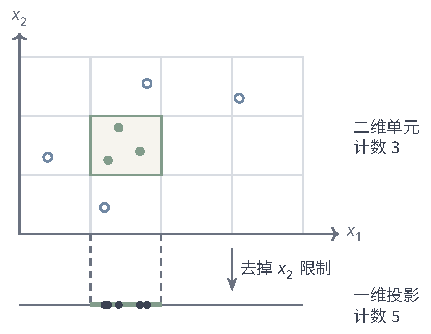
\includegraphics[width=72.912mm]{figures/03-models/01-classic-models/tikz/clustering-subspace/figure.pdf}
  \caption{CLIQUE 的投影计数示意。二维高亮单元含三个样本，其在横轴区间上的投影还包含其他纵坐标范围的样本。取共同阈值 $\tau=3$，二维单元密集必然推出对应一维单元密集，反方向则不成立。}
 \label{fig:clustering-subspace}
\end{figure}

\subsubsection{参数学习}

CLIQUE 借鉴 Apriori 的逐层候选生成。扫描数据找到一维密集单元后，把具有兼容低维区间的单元连接成更高维候选；只有所有低一维投影都密集的候选才继续计数验证。重复直到候选为空或达到搜索维数上限。

在保留下来的子空间中，算法连接相邻密集单元，形成簇，并可用轴对齐区域的析取式压缩簇描述。原始方法还包含选择子空间和简化描述的步骤；若使用额外启发式筛选，完整性应相对于筛选后的搜索范围表述。

\subsubsection{理论分析}

\paragraph{表达能力}
CLIQUE用轴对齐网格中的密集单元及其连通性表示子空间簇。网格与坐标选择限制边界精度，斜向或跨格稀释的结构可能需要更细网格和更高搜索成本。

\paragraph{收敛性}
CLIQUE 每轮增加候选的维数，最多搜索到 $d$ 维，因此在有限网格上必然结束。除了终止性，还需证明提前剪枝不会遗漏满足计数条件的高维单元；下面的向下封闭性给出这一保证。

\begin{theorem}[子空间密集性的向下封闭性]
 \label{thm:clustering-clique}
 在一致的逐维网格和共同计数阈值 $\tau$ 下，若 $S$ 上的单元 $U$ 密集，则对任意非空 $S'\subseteq S$，其投影 $U|_{S'}$ 也密集。
\end{theorem}
\begin{proof}
记 $I(U)=\{i:\bm{x}_{i,S}\in U\}$。若 $i\in I(U)$，它在 $S$ 的所有选定坐标上都满足区间限制，去掉部分坐标限制后仍然满足。因此
\[
 I(U)\subseteq I(U|_{S'}),\qquad
 n(U|_{S'})\geq n(U)\geq\tau.
\]
投影网格沿用相同区间，故 $U|_{S'}$ 是合法低维单元，并达到同一密集阈值。
\end{proof}

向下封闭性允许根据不密集的低维投影排除高维候选。多个投影各自密集时，其中的样本可能不同，所以高维计数仍需验证。该论证使用共同计数阈值；改为按体积归一的密度或随维数变化的阈值时，需重新核对剪枝条件。

有限网格保证搜索最终结束，但最坏情况下大量投影都密集，仍可能枚举指数多个子空间和单元。

\paragraph{泛化性}
样本中的密集单元能否代表总体群组，取决于抽样、网格和阈值。阈值附近的单元可能因少量样本改变而由密变稀，进而拆开或连接整个网格簇。验证时可重采样并平移网格，检查区域计数与连通结构；这项统计检验与候选剪枝的搜索完整性分工不同。

\subsubsection{小结}

CLIQUE为各簇保留相关坐标，并以向下封闭性减少无效候选。粗网格可能混合相邻群体，细网格可能稀释计数，轴对齐则限制可表达的子空间方向。MAFIA、SUBCLU与DOC/FASTDOC分别调整网格、密度连通和搜索，以处理这些限制。

\subsection{模型对比与总结}

STING建立可重复查询的空间摘要，CLIQUE发现不同坐标上的群组；两者分别节省原始样本访问与全维结构要求。可扩展性仍由摘要单元和候选规模限制。下面沿多分辨率、密度子空间和投影搜索三个方向继续比较。

WaveCluster把网格计数作为离散信号，在不同小波尺度寻找密集区域，并抑制部分高频噪声\scite{clust-sheikholeslami1998}。分辨率继续限定边界精度。固定维数、网格及变换规模时，读入成本可随样本数线性增长，网格变换和区域提取仍需单独计入。

SUBCLU在子空间中采用DBSCAN的密度连通，减少固定网格边界的影响；MAFIA用自适应区间调整候选，DOC与FASTDOC用随机抽样找投影中的紧凑群组\scite{clust-parsons2004}。各方法的邻域、阈值和候选条件不同，搜索保证需由对应定义建立。

\term{投影聚类}（projected clustering）通常要求每个样本有唯一簇归属，同时为每簇寻找相关子空间。PROCLUS 使用类似 K-medoids 的代表搜索并选择相关坐标；ORCLUS 进一步学习任意方向的低维正交投影，能够表达相对坐标轴倾斜的群组。前者偏向坐标子集，后者需估计方向，两者的计算与统计代价因此不同。

需要多个重叠解释时，可评价CLIQUE或SUBCLU；要求唯一簇归属及每簇相关坐标时，可评价投影方法。选择前还需核对数据是否存在所假设的低维集中结构，搜索算法只能从已有信息中恢复它。

\section{基于层次的聚类}
\label{sec:clustering-hierarchy}

探索阶段的群组粒度尚不明确时，可以保留多个层级。\term{层次聚类}（hierarchical clustering）用\term{树状图}（dendrogram）记录嵌套的合并或分裂，使分析者从同一棵树读取不同规模的划分。具体截取哪一层，仍由任务用途与证据确定。

凝聚方法从单点向上合并，分裂方法从全集向下拆分。图~\ref{fig:clustering-dendrogram}在同一棵树上读取两种粒度；截线保留已完成的层次决策，不对该粒度重新搜索。

\begin{figure}[htbp]
  \centering
  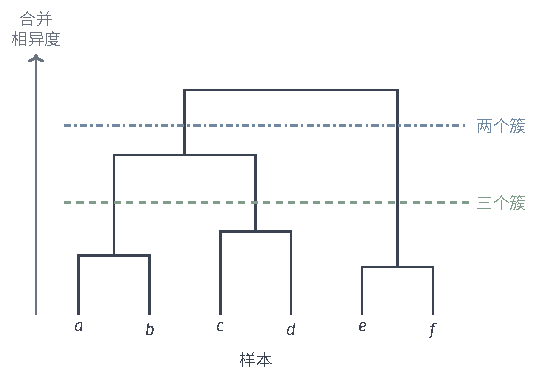
\includegraphics[width=90.914mm]{figures/03-models/01-classic-models/tikz/clustering-dendrogram/figure.pdf}
  \caption{教学用层次树。叶节点为六个样本，内部节点高度表示合并相异度。较低截线得到三个簇，较高截线得到两个簇；图中高度为示意数值。}
 \label{fig:clustering-dendrogram}
\end{figure}

\subsection{AGNES（凝聚层次聚类）}
\label{sec:clustering-agnes}

\term{凝聚分析}（Agglomerative Nesting, AGNES）每次合并当前相异度最小的两簇。Kaufman与Rousseeuw在1990年的专著中将这一长期用于数值分类学的过程与自顶向下的DIANA并列介绍。其主要设计问题是簇间相异度如何从样本关系计算。

链接准则把不同群组偏好写进合并决策：单链接沿最近联系扩展，平均链接综合跨簇距离，Ward在1963年以最小SSE增量选择合并。凝聚方向规定构造顺序，链接准则决定哪种关系先进入树。

\subsubsection{模型结构}

初始划分为 $\mathcal{P}^{(0)}=\{\{1\},\ldots,\{n\}\}$。第 $t$ 步选择使 $D(A,B)$ 最小的两个当前簇，替换为 $A\cup B$，经过 $n-1$ 次合并得到根节点。固定相异度和确定的平局规则后，整棵树随之确定。

不同\term{链接方式}（linkage）用不同的簇间统计量：
\begin{align*}
 D_{\mathrm{single}}(A,B)
   &=\min_{i\in A,j\in B}\delta(\bm{x}_i,\bm{x}_j),\\
 D_{\mathrm{complete}}(A,B)
   &=\max_{i\in A,j\in B}\delta(\bm{x}_i,\bm{x}_j),\\
 D_{\mathrm{average}}(A,B)
   &=\frac{\sum_{i\in A,j\in B}\delta(\bm{x}_i,\bm{x}_j)}
   {|A||B|}.
\end{align*}
单链接沿近邻链扩展，可以保留细长形状，也容易被稀疏桥接点连接起来；全链接控制跨簇最远距离，倾向紧凑群组；平均链接考虑所有跨簇样本对，减弱单个极值的影响。这里的平均链接指按样本数加权的 UPGMA。

若样本处于欧氏空间，Ward 链接以合并引起的 SSE 增量定义相异度：
\[
 D_{\mathrm{Ward}}(A,B)
 =\mathrm{SSE}(A\cup B)-\mathrm{SSE}(A)-\mathrm{SSE}(B).
\]
它与 K-means 共享平方误差准则，但只允许合并已有簇。Ward 的原始工作明确以这种误差增量组织层次\scite{ward1963}。

\subsubsection{参数学习}

实现 AGNES 时，可以维护当前簇间的相异度，并在每次合并后更新相关行列。算法~\ref{alg:clustering-agnes} 省去了不影响定义的矩阵下标管理。

\begin{algorithm}[凝聚层次聚类]
 \label{alg:clustering-agnes}
 \begin{algorithmic}[1]
 \Require 样本相异度、链接方式和确定的平局规则
 \Ensure 包含合并高度的层次树
 \State 建立 $n$ 个单点簇，初始化簇间相异度
 \While{当前簇数大于 $1$}
  \State 选择使 $D(A,B)$ 最小的当前簇对
  \State 记录子簇 $A,B$ 和合并高度 $D(A,B)$
  \State 用 $A\cup B$ 替换 $A,B$
  \State 更新新簇与其他当前簇的相异度
 \EndWhile
 \end{algorithmic}
\end{algorithm}

Lance--Williams 递推使多种链接共享更新形式\scite{clust-lance1967}。
\begin{equation}
 \begin{aligned}
 D(A\cup B,C)={}&\alpha_A D(A,C)+\alpha_B D(B,C)\\
 &+\beta D(A,B)
 +\gamma|D(A,C)-D(B,C)|.
 \end{aligned}
 \label{eq:clustering-lance-williams}
\end{equation}
单链接的系数为 $(1/2,1/2,0,-1/2)$，全链接为 $(1/2,1/2,0,1/2)$，平均链接为 $(|A|/(|A|+|B|),|B|/(|A|+|B|),0,0)$。若 $D$ 直接表示 Ward 的 SSE 增量，令 $s=|A|+|B|+|C|$，则
\[
 \alpha_A=\frac{|A|+|C|}{s},\quad
 \alpha_B=\frac{|B|+|C|}{s},\quad
 \beta=-\frac{|C|}{s},\quad \gamma=0.
\]
软件也可能存储Ward增量的缩放平方根；递推系数应与其距离约定配套。

朴素实现每轮扫描全部簇对，约需$O(n^3)$时间和$O(n^2)$存储。链接结构可减少搜索：SLINK的单链接为$O(n^2)$时间和$O(n)$辅助空间，CLINK提供全链接的紧凑表示；平均、全链接和Ward的最近邻链实现也可达到$O(n^2)$时间，常见实现仍保存平方规模距离矩阵\scite{clust-muellner2011}。采用这些算法时需沿用其链接和平局约定。

\subsubsection{理论分析}

\paragraph{表达能力}
AGNES用嵌套合并树表达层次分组，截取某一高度得到平面划分。不同链接偏好不同簇形状，早期合并不可撤销；一个树不可能同时表达所有彼此交叉的分组关系。

\paragraph{收敛性}
AGNES每次合并使簇数减一，因而有限终止。要解释优化性质，还需确定链接所比较的目标；下面证明Ward对当前下一次合并的最优性。

\begin{theorem}[Ward 合并的贪心最优性]
 \label{thm:clustering-ward}
 对欧氏样本的任一当前划分，Ward 链接选择使下一步总 SSE 增量最小的簇对；任意两个非空簇满足
 \[
 \Delta\mathrm{SSE}(A,B)
 =\frac{|A||B|}{|A|+|B|}
   \lVert\bm{\mu}_A-\bm{\mu}_B\rVert_2^2.
 \]
\end{theorem}
\begin{proof}
令 $a=|A|$、$b=|B|$，则合并均值为 $\bm{\mu}=(a\bm{\mu}_A+b\bm{\mu}_B)/(a+b)$。由式~\eqref{eq:clustering-mean-decomposition}，合并后的 SSE 等于两簇原有 SSE 加上
\[
 a\lVert\bm{\mu}_A-\bm{\mu}\rVert_2^2+
 b\lVert\bm{\mu}_B-\bm{\mu}\rVert_2^2.
\]
又有 $\bm{\mu}_A-\bm{\mu}=b(\bm{\mu}_A-\bm{\mu}_B)/(a+b)$，另一项为其相反方向的 $a/b$ 倍。代入后系数为 $(ab^2+ba^2)/(a+b)^2=ab/(a+b)$。其他簇不变，因此选择最小 Ward 相异度恰好最小化当前总 SSE 增量。
\end{proof}

Ward的最优性范围是当前可合并的簇对。截取$K$簇后，若再允许样本重新分配，可继续用K-means降低SSE；此时搜索范围已从合并已有簇扩展为逐点分配，因此结果可以不同。

单链接可由完整加权图的最小生成树解释：按边权递增连接，得到同一阈值连通结构，等权边可对应不同二叉表示。全链接比较跨簇最大距离，Ward比较总平方误差增量；各准则优化当前合并，整棵树由这些局部选择累积形成。

\paragraph{泛化性}
层次树描述当前样本关系。候选合并的相异度接近时，小幅数据变化可能改变早期合并，并影响更高层。可以重采样检查所关心群组是否反复出现；预测新样本则需另外规定插入或分配规则。固定输入下树的确定性与总体稳定性是不同对象。

\subsubsection{小结}

AGNES保留从细到粗的嵌套关系，便于探索不同粒度。链接规定几何偏好，单链接可沿非凸结构扩展；距离处理和不可撤销的合并则限制成本与结果。后续方法可压缩数据或调整合并准则，早期合并的影响仍需检验。

\subsection{DIANA（分裂层次聚类）}

希望先理解整个数据的几大部分时，可从树根向下拆分。\term{分裂分析}（Divisive Analysis, DIANA）先将全部样本置于一簇，再分裂最不一致的群组。它优先展示顶层结构，也使早期二分成为后续细分的边界。

\subsubsection{模型结构}

DIANA 通常用簇直径 $\max_{i,j\in C}\delta(\bm{x}_i,\bm{x}_j)$ 选择待分裂簇。每次把一个非单点簇拆成两个非空子簇；若展开完整树，恰需 $n-1$ 次分裂。若只需少数大簇，也可提前停止。

\subsubsection{参数学习}

对含 $m$ 个样本的簇，非平凡无序二分共有 $2^{m-1}-1$ 种，完整枚举很快变得昂贵。DIANA 用\term{分裂群}（splinter group）贪心构造二分：选取对其余样本平均相异度最大的样本作为种子，令其自成集合 $S$，其余样本组成 $R$。

对每个 $i\in R$，在 $|R|>1$ 时计算
\[
 a_i=\frac{1}{|R|-1}\sum_{\substack{j\in R\\j\ne i}}
 \delta(\bm{x}_i,\bm{x}_j),\qquad
 b_i=\frac{1}{|S|}\sum_{j\in S}\delta(\bm{x}_i,\bm{x}_j).
\]
若最大的 $a_i-b_i$ 为正，就把对应样本从 $R$ 移到 $S$，再更新这些量；否则结束分裂。这样每一步都选择更接近分裂群的最强候选，而非按任意顺序一次扫描。保留至少一个样本在 $R$ 中，避免产生空子簇。

\subsubsection{小结}

DIANA以分裂群启发式减少二分穷举，优先提供顶层结构。相异度、种子和平局影响分裂，距离缓存、簇规模与更新方式影响成本。比较AGNES时，应在相同数据与稳定性协议下检查关键群组，而非仅凭搜索方向推断哪种更稳。

\subsection{模型对比与总结}

AGNES合并已有小簇，DIANA划开已有大簇，均保留层次供事后选择粒度。合并只需比较当前簇对，分裂则在大量二分中采用启发式。希望解释的层级与相异度决定哪种构造更合适；下面的扩展进一步处理规模、形状和关系输入。

当数据装不进内存时，可先压缩再聚类。BIRCH 用\term{聚类特征}（clustering feature, CF）记录样本数、向量和与平方范数和\scite{clust-zhang1996}。这些摘要写为
\[
 \mathrm{CF}(C)=
 \left(|C|,\ \sum_{i\in C}\bm{x}_i,\
 \sum_{i\in C}\lVert\bm{x}_i\rVert_2^2\right).
\]
这些量可相加，也可恢复均值和簇内平方误差。CF树将邻近样本汇入摘要，再对叶摘要聚类。树高和摘要规模受控时，扫描成本近似随$n$线性增长；摘要阈值、插入顺序及压缩损失共同影响最终划分。

CURE 用多个分散代表点描述每簇\scite{clust-guha1998}。选择代表时，先选离均值较远的点，再逐个选择离已有代表集合较远的点，使代表覆盖簇的不同部分；随后把它们向均值收缩，以减弱孤立点影响。若原代表为 $\bm{r}$、簇均值为 $\bm{\mu}_C$，收缩后的代表可写为
\[
 \bm{r}'=(1-\alpha)\bm{r}+\alpha\bm{\mu}_C,
 \qquad 0\leq\alpha\leq1.
\]
两个簇的代表之间的最近距离用于决定合并。$\alpha=0$ 保留边缘形状，也更易受极端点影响；$\alpha$ 接近 1 时，代表逐渐退化为中心。CURE用抽样和分区减少参与完整层次搜索的对象，成本需同时计入抽样分配、代表更新及实际合并规模。

对类别属性，ROCK 用共同邻居所形成的链接数量替代单纯点间距离，其工作发表于 1999 年\scite{clust-guha1999}。它依然依赖邻居定义，且共享邻居统计会带来额外成本。

\Needspace{55mm}
Chameleon先在近邻图上形成子簇，再按相对互连度与相对相近度合并，使评价对应各簇的内部结构\scite{clust-karypis1999}。它调整当前合并的判据，已完成合并仍限制后续层次。

摘要、多个代表和关系图分别将规模、形状及连接信息纳入层次聚类，参数和近似方式决定各自代价。若还需说明样本属于某个生成成分的概率，则可进一步建立概率模型。

\section{基于概率的聚类}
\label{sec:clustering-probabilistic}

中心、密度连通与图割规定了群组结构。若任务还要求估计新样本来自某种群体的概率，可以假设样本先选择潜在成分，再由该成分分布生成。概率聚类据此共同估计分布参数和成分归属后验。

生成模型支持软归属、预测密度与模型比较。其成分含义需与任务群组核对：一个复杂形状的群体可能需要多个高斯近似，因此拟合密度所需的成分数与语义类别数可以不同。

\subsection{高斯混合模型（GMM）}
\label{sec:clustering-gmm}

\term{高斯混合模型}（Gaussian Mixture Model, GMM）以各成分均值与协方差表示不同方向和尺度的高斯分布。现代教材常结合EM说明其估计\scite{bishop2006}。混合表示与潜变量求解则来自不同历史阶段。

Pearson 在 1894 年的研究中，用两个正态分布的混合拟合一组生物测量数据，并通过矩方程估计参数\scite{clust-pearson1894}。关键想法是：观测到的一个总体，可能混合了多个未被直接标注的子总体。分布中的多个成分因此可以作为隐含群组的统计表示。

Wolfe在1970年将多元混合分析用于模式聚类，连接多维成分表示与似然估计\scite{clust-wolfe1970}。Dempster、Laird与Rubin在1977年提出一般EM框架，处理潜变量未观测时的参数更新。GMM规定生成分布，EM规定如何估计，两者可以分别改变。

GMM同时使用均值、协方差和成分权重。协方差决定偏离均值的方向尺度，权重决定成分的相对比例；样本归属由这些量的共同密度贡献确定，软后验因此包含比中心距离更多的信息。

\subsubsection{模型结构}

与第\ref{sec:classification-gda}节的 GDA 相比，两者都用高斯密度描述输入，但 GDA 的类别标签已经观测，可以按类直接估计；GMM 的成分归属不可观测，需要作为潜在成分变量推断。具体而言，先按权重 $\pi_k\geq0$、$\sum_k\pi_k=1$ 抽取潜在成分变量 $z_i\in\{1,\ldots,K\}$，再从 $\mathcal{N}(\bm{\mu}_{z_i},\bm{\Sigma}_{z_i})$ 抽取样本。要求 $\bm{\Sigma}_k\succ0$，边际密度为
\begin{equation}
 p(\bm{x};\bm{\theta})
 =\sum_{k=1}^K\pi_k
   \mathcal{N}(\bm{x};\bm{\mu}_k,\bm{\Sigma}_k),
 \label{eq:clustering-gmm}
\end{equation}
其中 $\bm{\theta}$ 汇集权重、均值与协方差。独立同分布样本的对数似然为
\[
 \ell(\bm{\theta})
 =\sum_{i=1}^n\log\left[
 \sum_{k=1}^K\pi_k
 \mathcal{N}(\bm{x}_i;\bm{\mu}_k,\bm{\Sigma}_k)\right].
\]
求和藏在对数内，使每个成分的参数无法独立优化。

给定参数后，贝叶斯公式给出\term{责任度}（responsibility），即当前模型认为样本由某成分产生的后验概率：
\begin{equation}
 \gamma_{i,k}
 =\frac{\pi_k\mathcal{N}(\bm{x}_i;\bm{\mu}_k,\bm{\Sigma}_k)}
 {\sum_{j=1}^K\pi_j
       \mathcal{N}(\bm{x}_i;\bm{\mu}_j,\bm{\Sigma}_j)}.
 \label{eq:clustering-responsibility}
\end{equation}
责任度每行和为1，可作为软归属；硬划分取$\argmax_k\gamma_{i,k}$并处理平局。概率含义对应当前生成模型中的成分，解释为任务类别还需核对模型与语义的关系。

图~\ref{fig:clustering-gmm-responsibilities}固定两成分模型。上图相加各加权密度，得到观测总密度；下图把各成分贡献除以总密度，得到$\gamma_k(x)=p(z=k\mid x;\bm{\theta})$。对称点$x=0$的责任度各为一半，其他位置连续变化。成分归属与总密度的峰数描述不同结构，两成分混合也可能只有一个峰。

\begin{figure}[tbp]
  \centering
  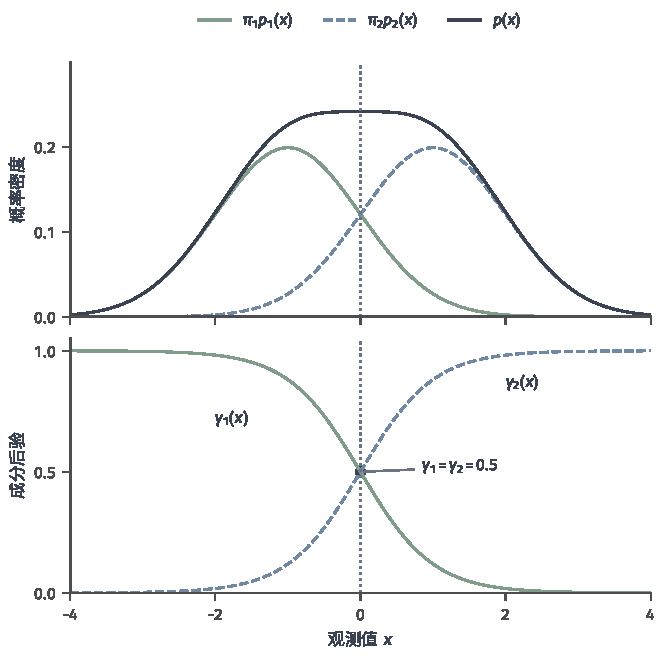
\includegraphics[width=105.412mm]{figures/03-models/01-classic-models/matplotlib/clustering-gmm-responsibilities/figure.pdf}
  \caption{两成分 GMM 的密度与软归属。设 $\pi_1=\pi_2=1/2$、$\mu_1=-1$、$\mu_2=1$，两个方差均为 1，$p_k(x)$ 表示第 $k$ 个高斯密度。上图展示加权成分密度及其和，下图展示同一观测值对应的后验；颜色与线型在两图中保持一致。}
 \label{fig:clustering-gmm-responsibilities}
\end{figure}

\subsubsection{参数学习}

\term{期望最大化}（Expectation-Maximization, EM）交替估计潜在成分变量的分布和优化参数，Dempster、Laird 与 Rubin 将这一原则统一为一般框架\scite{clust-dempster1977}。E 步用当前参数 $\bm{\theta}^{(t)}$ 计算式~\eqref{eq:clustering-responsibility}；M 步固定这些责任度，最大化完全数据对数似然的期望。潜在成分变量不再藏在对数的求和中，而是通过 E 步给出的分布参与加权。

忽略与参数无关的常数，M 步目标为
\begin{equation}
 \begin{aligned}
 Q(\bm{\theta}\mid\bm{\theta}^{(t)})
 =\sum_{i,k}\gamma_{i,k}^{(t)}
 \biggl[&\log\pi_k-\frac12\log\det\bm{\Sigma}_k\\
 &-\frac12(\bm{x}_i-\bm{\mu}_k)^\top
 \bm{\Sigma}_k^{-1}(\bm{x}_i-\bm{\mu}_k)\biggr].
 \end{aligned}
 \label{eq:clustering-gmm-q}
\end{equation}
记有效样本量 $n_k^{(t)}=\sum_i\gamma_{i,k}^{(t)}$。权重优化加入约束 $\sum_k\pi_k=1$ 的拉格朗日乘子，驻点满足 $n_k^{(t)}/\pi_k=\lambda$；求和得到 $\lambda=n$，所以
\begin{equation}
 \pi_k^{(t+1)}=\frac{n_k^{(t)}}{n},\qquad
 \bm{\mu}_k^{(t+1)}
 =\frac{\sum_i\gamma_{i,k}^{(t)}\bm{x}_i}{n_k^{(t)}}.
 \label{eq:clustering-gmm-mean}
\end{equation}
均值公式来自 $Q$ 对 $\bm{\mu}_k$ 的梯度为零：公共正定因子 $\bm{\Sigma}_k^{-1}$ 消去，剩下加权残差和为零。

再令精度矩阵 $\bm{\Lambda}_k=\bm{\Sigma}_k^{-1}$，加权散布为
\[
 \bm{S}_k=\sum_i\gamma_{i,k}^{(t)}
 (\bm{x}_i-\bm{\mu}_k^{(t+1)})
 (\bm{x}_i-\bm{\mu}_k^{(t+1)})^\top.
\]
相关目标为 $\tfrac12[n_k^{(t)}\log\det\bm{\Lambda}_k-\operatorname{tr}(\bm{\Lambda}_k\bm{S}_k)]$。求导得 $n_k^{(t)}\bm{\Lambda}_k^{-1}-\bm{S}_k=\bm{0}$，于是
\begin{equation}
 \bm{\Sigma}_k^{(t+1)}
 =\frac{\bm{S}_k}{n_k^{(t)}}.
 \label{eq:clustering-gmm-covariance}
\end{equation}
更新要求有效样本量为正。加权散布正定时，无约束协方差取得正定域内的有限最优；退化散布则需要协方差约束或其他估计。

代码~\ref{code:clustering-gmm}在对数域计算责任度，并用协方差特征值下界$\epsilon$避免塌缩。该截断求解固定约束$\bm{\Sigma}_k\succeq\epsilon\bm{I}$下的M步；每轮任意加常数矩阵则对应另一种估计，需另说明目标。

\begin{codeblock}[language=Python,label={code:clustering-gmm}]{带协方差下界的 GMM--EM}
import numpy as np
from scipy.special import logsumexp
from scipy.stats import multivariate_normal

def gmm_em(X, K, max_iter=100, tol=1e-5, eps=1e-6):
    X = np.asarray(X, dtype=float)
    n, d = X.shape
    if eps <= 0:
        raise ValueError("eps must be positive")
    _, mu = kmeans(X, K)
    pi = np.full(K, 1.0 / K)
    cov = np.repeat((max(1., eps) * np.eye(d))[None], K, axis=0)
    def e_step():
        log_p = np.column_stack([
            np.log(pi[k]) + multivariate_normal.logpdf(
                X, mean=mu[k], cov=cov[k])
            for k in range(K)])
        normalizer = logsumexp(log_p, axis=1)
        gamma = np.exp(log_p - normalizer[:, None])
        return gamma, normalizer.sum()
    gamma, ll = e_step()
    for _ in range(max_iter):
        nk = gamma.sum(0)
        if (nk <= 0).any():
            raise ValueError("numerically empty component")
        pi = nk / n
        mu = (gamma.T @ X) / nk[:, None]
        for k in range(K):
            diff = X - mu[k]
            S = (diff * gamma[:, k, None]).T @ diff / nk[k]
            values, vectors = np.linalg.eigh(S)
            cov[k] = (vectors * np.maximum(values, eps)) @ vectors.T
        gamma, new_ll = e_step()
        if abs(new_ll - ll) <= tol * (1 + abs(ll)):
            break
        ll = new_ll
    return pi, mu, cov, gamma
\end{codeblock}

该实现调用前文的 K-means，以其中心初始化，返回的责任度由最终参数重新计算。协方差特征值截断之所以是上述受限 M 步的解，是因为最优协方差与加权散布共享特征向量，每个特征值分别最小化 $\log s+\lambda/s$，在 $s\geq\epsilon$ 上得到 $s=\max\{\lambda,\epsilon\}$。计算中可同时记录似然变化、不同重启的目标和近空成分，以检查数值误差及初始化影响。

完整协方差保留全部二阶方向关系；类内有效样本不足时，可采用对角、球形或共享协方差减少自由度。完整形式一轮约需$O(nKd^2+Kd^3)$运算，立方项来自矩阵分解，对角形式的主要成本为$O(nKd)$。K-means++、重启和初始划分协方差可提供不同起点，其结果在同一约束与似然下比较。

\subsubsection{理论分析}

\paragraph{表达能力}
GMM用有限个高斯分量的混合表达密度。分量数、协方差限制与参数范围决定自由度；一个语义类别可以需要多个分量，一个分量也不能预先当作真实类别。

\paragraph{收敛性}
EM在旧参数处构造与观测似然相等的下界，再提高这一辅助目标。这样可避免直接优化对数内的成分求和；精确E步与M步改进条件共同给出似然不下降。

\begin{theorem}[EM 的似然单调性]
 \label{thm:clustering-em}
 E 步取当前精确后验，M 步满足
 $Q(\bm{\theta}^{(t+1)}\mid\bm{\theta}^{(t)})
 \geq Q(\bm{\theta}^{(t)}\mid\bm{\theta}^{(t)})$。
 在相关概率与期望有限、支持条件允许下，则
 $\ell(\bm{\theta}^{(t+1)})\geq\ell(\bm{\theta}^{(t)})$。
\end{theorem}
\begin{proof}
对每个样本，令$q_i$相对于当前参数下成分后验的KL散度有限，直接使用整体对数比形式（参考\BookSectionRef{sec:information-elbo-approximation}{第一卷“数学准备”的ELBO小节}）：
\[
 \begin{aligned}
 \mathcal L_i(q_i,\bm\theta)
 &=\sum_{k:q_i(k)>0}q_i(k)
    \log\frac{p(\bm x_i,z_i=k;\bm\theta)}{q_i(k)},\\
 \log p(\bm x_i;\bm\theta)
 &=\mathcal L_i(q_i,\bm\theta)
   +D_{\mathrm{KL}}\bigl(q_i\Vert p(z_i\mid\bm x_i;\bm\theta)\bigr).
 \end{aligned}
\]
对样本求和，把下界记为$\mathcal L(q,\bm\theta)$。该分解不要求$q_i$覆盖后验的全部支撑；
若改用恢复证据的Jensen等式，则必须另查相反方向的覆盖条件。
E 步令 $q_i^{(t)}$ 等于旧参数的后验，因此 $\mathcal{L}(q^{(t)},\bm{\theta}^{(t)})=\ell(\bm{\theta}^{(t)})$。固定 $q^{(t)}$ 后，下界与 $Q$ 仅相差不含参数的熵项，M 步遂给出
\[
 \begin{aligned}
 \ell(\bm{\theta}^{(t+1)})
 &\geq\mathcal{L}(q^{(t)},\bm{\theta}^{(t+1)})\\
 &\geq\mathcal{L}(q^{(t)},\bm{\theta}^{(t)})
 =\ell(\bm{\theta}^{(t)}).
 \end{aligned}
\]
这就证明了单调性。
\end{proof}

似然有上界时，EM的单调性可进一步给出似然值收敛。参数趋于驻点还需连续性、紧性等正则条件，Wu给出了相应分析\scite{clust-wu1983}。驻点可能是局部极大值或鞍点，优化解释应分别核对值的极限、参数极限和驻点类型。

当 $K\geq2$，且模型中存在一个可塌缩的正权重成分，其余正权重成分仍使其他样本的混合密度保持正值时，无约束 GMM 的似然没有上界。令可塌缩成分的均值等于某个样本，协方差为 $\sigma^2\bm{I}$；当 $\sigma\to0$ 时，该样本处的密度按 $\sigma^{-d}$ 增长，而其他样本仍由其余成分覆盖，因此总对数似然可以无界增加。若 $K=1$ 且样本经验散布矩阵正定，单高斯的最大似然有限；若经验散布矩阵奇异，协方差仍可能在数据未占据的方向趋近边界并导致似然退化。协方差下界、适当先验或惩罚可以阻止这类塌缩，但它们各自改变了优化问题。

潜在成分编号的置换不改变混合密度；当成分彼此不同且权重为正时，一个解通常对应 $K!$ 个等价标号。这与不同拟合质量的局部极值是两类问题。

\paragraph{泛化性}
新样本平均对数似然评价预测密度，训练似然描述经验拟合。成分数与协方差形式改变拟合能力，也改变估计所需样本；信息准则在同一约束下比较这种取舍。完整协方差的参数数目为
\[
 m_K=(K-1)+Kd+\frac{Kd(d+1)}{2},
\]
常用准则为
\begin{equation}
 \mathrm{BIC}(K)=-2\ell(\hat{\bm{\theta}}_K)+m_K\log n,
 \qquad
 \mathrm{AIC}(K)=-2\ell(\hat{\bm{\theta}}_K)+2m_K.
 \label{eq:clustering-bic}
\end{equation}
两个准则以惩罚参数量后的拟合选择候选，取较小值。BIC的证据近似需要渐近条件，而有限混合包含零权重边界、不可辨识和奇异参数。应用于混合阶数时，应核对专门的一致性条件\scite{clust-keribin2000}。

混合阶数说明所选分布族拟合数据需要多少成分。将其解释为语义类别数，还需外部知识或验证表明一个类别与一个成分对应。

\subsubsection{小结}

GMM以软后验、协方差与预测密度支持概率聚类，也可用于语音建模和异常评分。分布失配、似然奇异与局部求解影响估计；增加高斯成分可改善密度表达，同时增加解释每个成分的负担。

\subsection{模型对比与总结}

GMM的软归属、权重与协方差共同定义后验，K-means只使用中心平方距离。固定部分参数并取小方差极限，可以明确两种目标和更新的联系。固定均匀权重 $\pi_k=1/K$ 和共享球形协方差 $\bm{\Sigma}_k=\sigma^2\bm{I}$，则
\[
 \gamma_{i,k}=
 \frac{\exp(-\lVert\bm{x}_i-\bm{\mu}_k\rVert_2^2/(2\sigma^2))}
 {\sum_j\exp(-\lVert\bm{x}_i-\bm{\mu}_j\rVert_2^2/(2\sigma^2))}.
\]
若 $\bm{x}_i$ 的最近中心唯一为 $k^\ast$，则对任意 $j\ne k^\ast$，距离平方差为正，相应指数比随 $\sigma^2\to0$ 趋零，故 $\gamma_{i,k^\ast}\to1$。M 步的均值更新因此退化为 Lloyd 更新；平局时责任度可分散在多个最近中心，不能直接得到唯一硬簇分配。

去掉只依赖$\sigma$的常数，目标$-2\sigma^2\ell$趋向$\sum_i\min_k\lVert\bm{x}_i-\bm{\mu}_k\rVert_2^2$，给出平方误差的联系。这一极限固定均匀权重并缩小共享球方差；自由协方差GMM优化更大的分布族。FCM的软隶属度则来自模糊损失，与生成后验采用不同定义。

更换成分分布即可适配其他数据：伯努利混合适合二值特征，多项式混合适合计数向量；重尾的 $t$ 混合可减轻离群观测对均值和尺度估计的影响，其代价是引入额外的尺度或自由度估计\scite{clust-peel2000}。

\term{狄利克雷过程混合}（Dirichlet process mixture, DPM）为随机混合分布设置Dirichlet过程先验，使潜在成分数随数据和后验变化。总质量参数控制新增成分的倾向，折棒表示及后验预测见第\ref{sec:pgm-static-directed-hierarchy-membership}节；Neal研究了相应MCMC推断\scite{clust-neal2000}。模型省去固定$K$，仍需选择先验并核对潜在成分与任务类别的关系。

概率路线在同一生成模型下计算归属、预测密度和模型比较。所需输出及分布假设决定是否采用它；与几何或密度方法比较时，还需先确定共同的使用目标。

\section{基于集成的聚类}
\label{sec:clustering-ensemble}

不同初始化、表示或算法可能在同一批对象上产生多份划分。\term{共识聚类}（consensus clustering）统计每对对象在多少份划分中共簇，形成共关联矩阵，再聚类该矩阵或对应图\scite{clust-strehl2002}。这一机制把候选间的共同结构汇为一个新输入，也可用于诊断反复出现的群组。

直接比较共关联矩阵要求对象集固定。重采样改变对象集时，可只比较共同对象，或先冻结新样本分配规则，再将候选应用到相同评价对象；协议见表\ref{tab:clustering-evaluation-protocol}。独立样本没有共同对象时，应预定候选生成方式，改为比较簇轮廓、外部关联或用途指标。

共识本身仍由候选产生。同一数据上的反复筛选不会补充外部验证，多数划分也可能淹没少数有意义的结构。报告时应保留共关联强度、候选来源，以及在独立评价中相对无聚类基线的收益。

\section{半监督聚类}
\label{sec:clustering-semisupervised}

未标注数据也可能附有部分领域知识。例如，专家知道两条记录来自同一对象，知道一对样本应分开，或能给出少量典型种子。\term{半监督聚类}（semi-supervised clustering）将这些信号用于以未标注样本为主体的分组。

第\ref{sec:classification-semisupervised}节的半监督分类利用未标注输入改进预先定义类别的预测，本节则用少量类别标签或关系先验共同决定分组。两者都改变可用监督信息，却保留不同的任务目标。

实例级信号常写为\term{必连约束}（must-link）和\term{勿连约束}（cannot-link）：前者要求两个样本同簇，后者要求异簇。记其索引对集合为 $M$ 和 $B$，以免与簇 $C_k$ 或划分 $\mathcal{P}$ 混淆。信号既可作为硬约束，也可带权违反；少量关系判断是否比逐点类别标签更容易获取，取决于实际标注任务。

这些信号与几何结构共同确定群组。需要检验的是先验是否消除了原模型的歧义，覆盖了哪些样本，以及是否与基础几何发生冲突；信号质量和作用范围决定其可能收益。

\subsection{COP-K-means}
\label{sec:clustering-cop}

关系被视为硬事实时，分配必须避开与它们冲突的簇。Wagstaff等在2001年提出COP-K-means，将最近中心选择限制在当前可行选项内\scite{clust-wagstaff2001}。这既改变候选分配，也引入可行性与访问顺序问题。

\subsubsection{模型结构}

目标仍为式~\eqref{eq:clustering-sse}，可行域增加
\begin{equation}
 c_i=c_j\quad((i,j)\in M),\qquad
 c_i\ne c_j\quad((i,j)\in B).
 \label{eq:clustering-cop}
\end{equation}
must-link 的传递闭包把样本分成\term{约束块}（chunklet），同一块必须整体分配。若 cannot-link 的两端落在同一块内，约束立即矛盾；但不存在这种矛盾还不足以保证给定 $K$ 下可行。

把每个约束块当作顶点、cannot-link 当作边，块的簇分配实际上是该图的 $K$ 着色。例如三个两两 cannot-link 的块不能放进两个簇，即使没有任何 must-link 冲突。块级 SSE 可分解为块内常数加上“块大小乘以块均值到中心的平方距离”，因此整体分配也能利用摘要。

\subsubsection{参数学习}

COP-K-means 按某个顺序处理样本或约束块，对候选簇按距离排序，接受第一个与已固定分配相容的簇。若没有候选，就报告本次贪心分配失败；更新步则对每个非空簇取均值。

\begin{algorithm}[COP-K-means 的约束块分配]
 \label{alg:clustering-cop}
 \begin{algorithmic}[1]
 \Require must-link 闭包、块间 cannot-link、当前中心
 \Ensure 本轮可行分配，或本轮贪心失败
 \State 清空本轮簇分配，选定约束块访问顺序
 \For{每个约束块 $U$}
  \State 按 $\sum_{i\in U}\lVert\bm{x}_i-\bm{\mu}_k\rVert_2^2$ 排序候选簇
  \State 选择不与已分配邻块冲突的最近候选
  \If{候选不存在}
   \State 返回本轮失败
  \EndIf
  \State 把 $U$ 的全部样本分给所选簇
 \EndFor
 \end{algorithmic}
\end{algorithm}

贪心失败可能来自顺序，而非约束本身。以cannot-link路径$a-b-c-d$和$K=2$为例：按$a,d,b,c$访问，若$a,d$先取簇1，$b$只能取簇2，$c$便无可行选择。整体划分$\{a,c\}$与$\{b,d\}$却满足全部关系，说明局部已定选择阻碍了后续分配。

逐块贪心未精确求解固定中心的整体约束分配，Lloyd的下降前提在这里需要重新建立。可从已有可行解出发，只接受可行且降低目标的块移动；也可精确求解受约束分配，再更新均值。前者搜索范围较小，后者增加组合优化成本。普通COP实现可用迭代上限、失败记录及重启或回溯处理这些情况。

\subsubsection{小结}

COP-K-means 的好处是约束含义明确，成功输出可以逐项检查是否满足关系。代价是约束冲突、给定 $K$ 下不可行以及贪心顺序失败都必须处理。若先验允许出错，PCK-means 在 SSE 上增加
\[
 \sum_{(i,j)\in M}w_{i,j}^{M}\mathbb{1}\{c_i\ne c_j\}
 +\sum_{(i,j)\in B}w_{i,j}^{B}\mathbb{1}\{c_i=c_j\},
\]
以软惩罚权衡几何和约束。有限权重不保证零违反，但避免因单条错误关系直接拒绝整个问题。

\subsection{Seeded / Constrained K-means}
\label{sec:clustering-seeded}

若已知的是少量样本的类别名称，可以直接用它们确定初始中心或固定归属。Basu、Banerjee 与 Mooney 在 2002 年研究了 Seeded K-means 与类别标签约束的 Constrained K-means\scite{clust-basu2002}。后者与第~\ref{sec:clustering-capacity} 节的同名容量约束方法含义不同：本节锁定种子的类别标签，容量方法限制各簇样本数。

\subsubsection{模型结构}

设种子索引集合为 $S$，类别标签为 $\ell_s\in\{1,\ldots,K\}$，并记 $S_k=\{s\in S:\ell_s=k\}$。当每类都有种子时，初始化为
\[
 \bm{\mu}_k^{(0)}
 =\frac{1}{|S_k|}\sum_{s\in S_k}\bm{x}_s.
\]
缺少种子的簇需另外初始化。Seeded 版本只在初始化时使用类别标签，之后种子可以移动；Constrained 版本始终要求 $c_s=\ell_s$，把种子类别标签作为硬事实。二者都优化同一个平方误差目标，只是初始化与可行域不同。

\subsubsection{参数学习}

Seeded 版本随后直接运行 Lloyd。Constrained 版本在分配步冻结种子，其余样本独立选择最近中心；更新中心时同时计入种子和非种子。由于冻结限制彼此不耦合，逐点分配仍是固定中心下的精确最优解，因此可沿用定理~\ref{thm:clustering-lloyd} 的下降论证与平局条件。每簇都有固定种子时，还自然避免了空簇。

种子确定了部分群组的名称与初始位置，其代表性仍影响结果。允许种子移动，可以缓解错误标签的永久锁定；可靠标签与模糊几何并存时，冻结种子更能保留监督关系。选择哪种方式，应按种子覆盖、比例和错误类型，在未参与拟合的证据上比较。

\subsubsection{小结}

种子方法通过初始化或固定归属引入少量类别标签，适合每类已有代表样本的任务。距离与均值继续规定几何；若监督还需改变特征方向的重要性，可以进一步学习度量。

\subsection{MPCK-means}
\label{sec:clustering-mpck}

如果重要特征与无关特征混在一起，约束即使改变了簇分配，也未必能改变下一轮的距离判断。Bilenko、Basu 与 Mooney 在 2004 年提出的 MPCK-means（Metric Pairwise Constrained K-means）同时优化分配和簇相关度量，使关系约束既影响簇分配，也影响空间中的方向与尺度\scite{clust-bilenko2004}。

弱监督可以进入不同环节：关系限制可行分配，种子确定初始位置或成员，成对约束还可学习方向与尺度。这些形式对应不同的先验内容和可信程度，可按信号实际支持的判断选择。

\subsubsection{模型结构}

为簇 $k$ 配置正定矩阵 $\bm{A}_k\succ0$，定义平方 Mahalanobis 距离
\[
 d_{\bm{A}_k}^2(\bm{x},\bm{y})
 =(\bm{x}-\bm{y})^\top\bm{A}_k(\bm{x}-\bm{y}).
\]
正定性既保证非退化距离，也使 $\log\det\bm{A}_k$ 有定义。可以把这种距离看作先做坐标变换 $\tilde{\bm{x}}=\bm{A}_k^{1/2}\bm{x}$，再计算欧氏距离。图~\ref{fig:clustering-metric-constraints} 给出了一个固定变换的例子：压缩水平方向、拉伸竖直方向后，must-link 对变近，而 cannot-link 对变远。实际 MPCK-means 需要根据全部样本与约束优化 $\bm{A}_k$，并非预先知道图中的变换。

\begin{figure}[htbp]
  \centering
  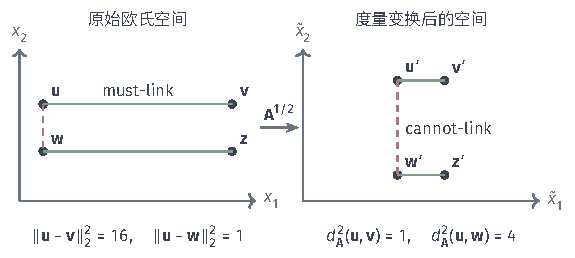
\includegraphics[width=97.331mm]{figures/03-models/01-classic-models/tikz/clustering-metric-constraints/figure.pdf}
  \caption{度量如何改变成对关系的几何表达。四点为 $\bm{u}=(-2,0.5)$、$\bm{v}=(2,0.5)$、$\bm{w}=(-2,-0.5)$、$\bm{z}=(2,-0.5)$。实线连接 must-link 对，虚线连接 cannot-link 对。这里人为设定 $\bm{A}=\operatorname{diag}(1/16,4)$；右图的距离等于左图的 Mahalanobis 距离，不表示一次真实训练的结果。}
 \label{fig:clustering-metric-constraints}
\end{figure}

记在该度量下全数据的最大距离平方为
\[
 D_k=\max_{p,q\in\{1,\ldots,n\}}
 d_{\bm{A}_k}^2(\bm{x}_p,\bm{x}_q).
\]
对违反 must-link 的样本对，惩罚同时作用于两端所属簇；对违反 cannot-link 的样本对，惩罚其相对于本簇度量下最远样本对的接近程度。具体写为
\begin{align}
 f_M(i,j)
 &=\frac12\left[
 d_{\bm{A}_{c_i}}^2(\bm{x}_i,\bm{x}_j)
 +d_{\bm{A}_{c_j}}^2(\bm{x}_i,\bm{x}_j)\right]
 \mathbb{1}\{c_i\ne c_j\},\nonumber\\
 f_B(i,j)
 &=\left[D_{c_i}
 -d_{\bm{A}_{c_i}}^2(\bm{x}_i,\bm{x}_j)\right]
 \mathbb{1}\{c_i=c_j\}.
 \label{eq:clustering-mpck-penalty}
\end{align}
因此 cannot-link 惩罚非负，must-link 惩罚也不因交换样本对的书写顺序而改变。总目标为
\begin{equation}
 \begin{aligned}
 J={}&\sum_{k=1}^K\sum_{i\in C_k}
 \left[d_{\bm{A}_k}^2(\bm{x}_i,\bm{\mu}_k)
       -\log\det\bm{A}_k\right]\\
 &+\sum_{(i,j)\in M}w_{i,j}^{M}f_M(i,j)
  +\sum_{(i,j)\in B}w_{i,j}^{B}f_B(i,j).
 \end{aligned}
 \label{eq:clustering-mpck}
\end{equation}
权重均非负，每个无序约束对只计一次。负对数行列式阻止特征值趋零，但不能单独阻止矩阵某些方向无限放大；数据退化时仍需约束或正则。

\subsubsection{参数学习}

固定中心和度量时，对一个样本的各簇候选计算完整目标变化，包括几何、行列式及所有相关关系惩罚，再接受不增目标的变更。由于关系项耦合样本，单独比较到中心的距离不足以完成这项选择。

固定分配和度量时，约束项不含中心。对中心求导给出
\[
 2\bm{A}_k\sum_{i\in C_k}(\bm{\mu}_k-\bm{x}_i)=\bm{0},
 \qquad
 \bm{\mu}_k=\frac{1}{|C_k|}\sum_{i\in C_k}\bm{x}_i.
\]
同一簇共用的$\bm{A}_k$在驻点方程中消去，中心因而取普通簇内均值。若需按样本重要性加权，还要在目标中另加相应权重。

度量步可借助散布矩阵理解。令 $\bm{S}_k=\sum_{i\in C_k}(\bm{x}_i-\bm{\mu}_k)(\bm{x}_i-\bm{\mu}_k)^\top$。在固定当前最远样本对、且该样本对在更新后仍保持活跃的一个分支上，约束项写成 $\operatorname{tr}(\bm{A}_k\bm{P}_k)$，其中 $\bm{P}_k$ 汇总违反 must-link 的半权重差分外积，以及违反 cannot-link 的“最远对外积减约束对外积”。于是子目标为
\[
 \operatorname{tr}\bigl(\bm{A}_k(\bm{S}_k+\bm{P}_k)\bigr)
 -|C_k|\log\det\bm{A}_k.
\]
若 $\bm{S}_k+\bm{P}_k\succ0$ 且 $|C_k|>0$，其无约束驻点为
\begin{equation}
 \bm{A}_k=|C_k|(\bm{S}_k+\bm{P}_k)^{-1}.
 \label{eq:clustering-mpck-metric}
\end{equation}
这个驻点式适用于正定的调整散布及保持活跃的最远对分支；更新后需再次核对这两个条件。

保留 $D_k$ 对 $\bm{A}_k$ 的真实依赖时，它是有限个线性函数的最大值，故固定分配和中心的度量子问题是凸的，但通常分段光滑。可在 $\alpha\bm{I}\preceq\bm{A}_k\preceq\beta\bm{I}$、$0<\alpha<\beta$ 的固定域上求解，或使用保持正定且实际下降的优化步骤。对角度量进一步减少参数与矩阵计算。

各步在同一有下界的目标上不增，可推出目标值收敛。度量属于连续参数，即使簇分配不再变化，它也可能继续更新；有限分配数因此不足以证明有限轮停止。实际终止可结合目标和参数变化的容差，并明确空簇处理。

\subsubsection{小结}

MPCK-means用成对监督调整几何，同时估计分配与每簇度量。ITML、LMNN也学习度量，但采用不同损失和训练约束，相关工具需按目标分别使用。每簇完整矩阵有$d(d+1)/2$个自由参数，监督较少或维数较高时可共享或取对角，以降低估计容量。

\subsection{模型对比与总结}

COP限制实例关系，种子方法引入类别名称，MPCK-means将关系用于学习几何。硬约束要求输出完全满足，软权重则允许以违反换取其他拟合收益。选择前应明确信号的可信程度与覆盖；增加度量参数还需要足够监督支持。下面再比较信号进入图与共享度量的方式。

先验也可加入谱聚类。Kamvar、Klein 与 Manning 的 Spectral Learning 研究了将监督信息纳入谱表示；一种直接做法是提高 must-link 边权、降低 cannot-link 边权，再对修改后的非负对称图求谱表示\scite{clust-kamvar2003}。

边权调整改变谱偏好，最终分配仍由整张图和离散化决定。即使删除cannot-link边，两端也可能通过其他强边共簇。修改后的非负对称图可按其新拉普拉斯分析，但谱间隙、连接及统计条件需重新核对。关系传播还能扩展局部监督，同时可能扩散错误信号。

Xing 等通过相似与不相似样本关系学习 Mahalanobis 度量\scite{clust-xing2003}。这是先单独学习共享度量、再交给聚类算法的解耦方式。这样可以复用监督得到的几何结构，但共享度量仍假设所有簇使用同一种空间变换，后续算法也须与该度量兼容。

半监督聚类应评价先验是否解决了原模型无法区分的选择。可同时报告几何目标、关系违反，以及独立参考标签或下游任务中的结果；训练关系的满足度描述监督拟合，独立评价再检查其用途与泛化。

\section{模型选择与评价}
\label{sec:clustering-evaluation}

\subsection{方法比较}

原型方法比较样本与代表的相异度，邻域和图方法从局部连通关系形成群组，网格与子空间方法改变比较单位，层次方法保留多个粒度，概率方法解释软归属，集成则汇总多份分组。表\ref{tab:clustering-navigation}对照这些簇判据及输出条件；HDBSCAN等方法可以同时涉及邻域与层次。

\begin{table*}[htbp]
  \centering
  \small
  \begin{tabularx}{\linewidth}{@{}>{\RaggedRight\arraybackslash}p{22mm}*{5}{>{\RaggedRight\arraybackslash}X}@{}}
    \toprule
    代表方法 & 簇判据 & 输出粒度 & 表示或相异度 & 优化或推断机制 & 监督信息 \\
    \midrule
    K-means、K-medoids & 到原型的总相异度 & 给定$K$的平坦硬划分 & 数值向量上的平方距离；一般对象相异度 & 交替更新；代表交换 & 无 \\
    DBSCAN、OPTICS、HDBSCAN、Mean Shift & 密度连通或模态吸引域 & 噪声、排序、层次或模态簇 & 邻域距离或核密度 & 区域扩展、排序、树压缩或模态搜索 & 无 \\
    谱聚类、AP、Louvain & 图割、代表支持或模块度 & 平坦划分；簇数可显式或间接控制 & 原生图或由相似度构造的加权图 & 特征松弛、消息传递或局部移动 & 无 \\
    STING、CLIQUE、投影聚类 & 密集单元或低维紧凑性 & 区域、重叠子空间或硬划分 & 网格、坐标子集或学习的投影 & 摘要查询、候选搜索或代表迭代 & 无 \\
    AGNES、DIANA & 链接或分裂准则 & 嵌套层次，事后截取 & 点或簇间相异度 & 贪心合并或启发式分裂 & 无 \\
    GMM、DPM & 生成成分及其后验 & 平坦软归属；成分数固定或随机 & 数值向量及指定分布族 & EM、MCMC或变分推断 & 先验不等同于类别标签 \\
    共识聚类 & 多份分组的共同结构 & 通常为平坦划分 & 共簇关系或超图 & 共识函数、图划分等 & 依赖成员所用信息 \\
    COP、Seeded、MPCK-means & 基础簇判据加关系或种子约束 & 通常为平坦硬划分 & 原始或学习的度量、约束图 & 受限分配、初始化或度量学习 & 成对关系、种子或少量类别标签 \\
    \bottomrule
  \end{tabularx}
  \caption{聚类方法的属性导航。每行登记代表方法在五项属性上的基本设定，不把各主体节解释成互斥类别；方法的具体变体可能改变其中一项或多项。}
  \label{tab:clustering-navigation}
  \label{tab:clustering-overview}
\end{table*}

\subsection{评价与选择}

\paragraph{表示与相异度}
客户变量的类型与尺度先规定可比较的相异度。测量协议可以预定尺度，也可以从数据估计标准化；后一种做法改变各坐标在距离中的权重，需要对应任务含义。类别变量可比较取值是否相同，序数变量还需说明等级间距。

数值与类别混合时，可将每个变量的相异度变到可比范围，再按给定权重汇总。Gower系数采用这一构造，对每个样本对只使用共同观测的变量，并按对应权重归一化\scite{clust-gower1971}。数据估计的尺度、插补、范围和权重在下文的发现数据上拟合，再冻结用于验证。

索引或近似算法若使用三角不等式，需要确认所选相异度满足它。图方法还需规定单向近邻的对称化、边权缩放与孤立点处理。这些规则改变距离或连接，也会改变“同一簇”的具体含义。

\paragraph{发现与验证}
算法停止、目标值收敛和参数收敛描述计算；训练外是否出现有用群组则是验证问题。为分别获得这两种证据，可划分\term{发现数据}（discovery data）与\term{验证数据}（validation data）。发现数据用于估计表示、尺度和相异度，拟合候选并选择簇数或超参数；查看验证结果前，固定方法、簇匹配、指标及用途判断。

验证数据可来自同源留出或独立收集。时间、地点和个体相关数据应按未来使用单位划分，减少相关记录跨集合带来的泄漏。Ullmann、Hennig与Boulesteix系统讨论了复核聚类的验证方式\scite{clust-ullmann2022}。

表\ref{tab:clustering-evaluation-protocol}按问题安排六种证据。训练目标、稳定性和零模型可在发现阶段用于诊断；独立外部标签检验指定语义，留出拟合与下游效用检验样本外用途。候选较多时，可在发现数据内部嵌套划分或交叉验证，将最终验证保留到规则固定之后。

稳定性测量重采样或参数变化的影响，也受目标唯一性和数据对称性控制\scite{clust-ben-david2006}。解释它时，还需核对簇含义与用途。零模型则规定“没有所关心结构”时保留哪些数据特征；Gap Statistic将观测簇内离差与参考分布比较，是其中一种构造\scite{clust-tibshirani2001-gap}。

校准零模型证据时，每份模拟数据都应重跑与观测数据相同的完整流程，包括预处理、拟合、候选搜索及选择。这样才将选择本身的影响纳入参考分布；仅固定某一结果再模拟，可作为探索基线，证据对象相应较窄。

内部指标解释当前拟合，也带有自身的几何偏好。SSE评价中心量化，\term{轮廓系数}（silhouette coefficient）比较同簇平均距离与最近其他簇平均距离，评价相对紧凑程度\scite{clust-rousseeuw1987}。跨方法比较时，应先确认这种几何与共同目标相符。

\term{调整兰德指数}（adjusted Rand index, ARI）比较同一批对象在两份划分中的共簇与异簇关系，并在固定簇大小的随机划分下校正期望一致性\scite{clust-hubert1985}。它对簇编号置换不变，可比较重复运行，也可比较独立参考标签。后者检验指定外部语义，其他合理群组仍需不同证据。

\begin{table*}[htbp]
  \centering
  \small
  \begin{tabularx}{\linewidth}{@{}>{\RaggedRight\arraybackslash}p{21mm}>{\RaggedRight\arraybackslash}p{43mm}>{\RaggedRight\arraybackslash}X>{\RaggedRight\arraybackslash}X@{}}
    \toprule
    证据 & 最小执行协议 & 可以回答 & 不能单独推出 \\
    \midrule
    训练目标 & 在发现数据上记录SSE、似然、图目标或约束违反，并只与相同目标和约束下的候选比较 & 求解是否满足方法声明的经验准则 & 语义正确、跨目标优越或样本外有效 \\
    稳定性 & 对象集固定而只改变测量、初始化或关键参数时，比较共簇关系或标签置换不变的分区指标；样本重采样改变对象集时，只比较共同对象，或冻结新样本分配规则后再比较 & 哪些群组依赖少量样本、随机性或参数 & 正确簇数或业务语义；稳定性本身也可能来自唯一目标或数据对称性 \\
    外部标签 & 标签不参与无监督拟合与选择；在验证数据上按预先规定的总体或子群计算ARI等指标 & 与指定外部语义的一致程度 & 标签之外的其他合理结构，或无标签任务中的唯一真解 \\
    零模型 & 先说明要保留的边际、范围或相关结构；在每份模拟数据上重跑相同的预处理、拟合、候选搜索和选择规则；未重跑完整管线时只作为探索性基线 & 观察到的分离是否超出该无簇基线；Gap Statistic是一个实例 & 拒绝所有其他零模型，或证明所得簇具有用途 \\
    留出证据 & 用发现数据拟合表示和模型，按冻结的新样本分配规则评价留出量化误差或预测对数密度 & 指定模型在同一数据制度下的样本外拟合 & 不同簇概念之间的统一优劣；无样本外规则的方法须先定义映射 \\
    下游效用 & 冻结簇提取流程，在嵌套验证中与无聚类或更简单基线比较检索、描述或决策损失 & 群组是否改善预先声明的实际用途 & 群组在其他用途或总体上仍然有效 \\
    \bottomrule
  \end{tabularx}
  \caption{聚类结果的评价协议。发现阶段可以生成和筛选候选；最终验证数据只在表示、算法、超参数和比较规则冻结后使用。每类证据回答不同问题，指标的几何偏好和数据依赖必须随结果报告。}
  \label{tab:clustering-evaluation-protocol}
\end{table*}

不同证据可能支持不同结论。SSE更低而下游损失更高，说明量化目标与用途存在偏离；稳定性高但与零模型相近，说明重复出现的结构还缺少超出参考基线的证据；外部标签一致但预测密度较差，则提示标签与生成族可能不对应。

结论应对应预定群组和用途，同时保留这些差异。指标本身也偏好特定形状与粒度，Handl等的比较强调按验证问题选择证据\scite{clust-handl2005}。


聚类公理还依赖输出形式。Kleinberg对固定对象、成对距离输入与单一划分输出证明：尺度不变性、丰富性和一致性无法同时成立\scite{clust-kleinberg2002}。它揭示这一设定的要求冲突；软归属、重叠和层次使用其他输出约束。流式、多视图与神经聚类还改变数据或表示，其验证也需对应实际设定。

前述理论分别约束具体计算。Lloyd用下降和平局规则证明有限停止，Ward比较一次合并，DBSCAN固定核心点分量。Mean Shift和EM先给目标单调，再以附加条件讨论参数；谱松弛控制连续子问题，CLIQUE保证特定计数剪枝完整。实现时可用这些对象核对算法步骤，再另行检验样本外结构。

聚类扩展回应不同需求。样本规模推动小批量、抽样与摘要，以近似或顺序影响换取计算；非凸形状推动密度连通、核和谱，同时增加邻域与构图选择；关系输入使中心样本与图目标直接使用对象联系，也引入距离存储和图计算。

高维数据推动子空间与投影搜索，代价是组合候选和方向估计。概率语义带来软后验、预测密度及模型比较，同时需要处理分布失配、奇异性和局部推断。弱监督用关系或种子消除部分歧义，其覆盖不足和错误又可能影响多个样本。

这些变化处理不同压力，可组合使用。验证进一步检查所改机制是否带来预定收益，按零模型、重复性、独立数据及用途取得证据；方法的适用条件由这一问题链确定。

客户分群应先规定用途。量化关注表示误差，探索关注可重复结构，解释关注群组与外部语义，下游决策关注实际损失。用途确定后，再选择变量尺度、相异度或邻接、簇判据、输出粒度及可用先验。

快速数值量化可从K-means开始，真实代表与一般相异度可用K-medoids，多层解释可用层次树。低密度分隔和噪声识别可评价DBSCAN、OPTICS或HDBSCAN；关系数据先解释边权，再选择图目标。相关坐标因簇变化时可搜索子空间，概率输出重要时可拟合混合，已有可靠知识时可加入关系或种子。

候选确定后，按表\ref{tab:clustering-evaluation-protocol}取得相应证据：留出量化误差检验数值拟合，稳定性与零模型检验探索结构，独立关联检验语义，相对无聚类基线的损失检验决策收益。由此说明哪些客户、数据条件和用途支持当前分组。

\Needspace{18\baselineskip}
\section{本章小结}
\label{sec:clustering-summary}

聚类通过结构假设定义群组。原型限定中心周围的相异度，邻域和图限定连接，网格与子空间限定相关区域，层次限定嵌套关系，概率模型限定生成成分，集成汇总候选共同结构。关系与种子监督再减少其中部分歧义。

算法求解与群组用途需要不同证据。目标下降和停止支持计算解释，训练外量化、密度、语义或决策结果支持使用结论；稳定性及零模型补充结构检验。粒度由$K$、密度阈值、带宽、截线或先验控制，均需随任务选择。

第\ref{chap:dimensionality-reduction}章将学习低维表示，这会同时改变距离、密度和邻接。可视化提供探索线索，群组判断仍需在原始或经验证的表示上取得与用途对应的证据。

\paragraph{扩展阅读}
Bishop第9章从潜变量解释混合与EM，Hastie等在无监督学习中比较距离、原型及层次\scite{bishop2006,hastie2009}。进一步阅读可选同一数据问题，分别写出簇定义、迭代目标与新样本评价，比较不同假设怎样改变最终群组。
\chapter{降维}
\label{chap:dimensionality-reduction}

基因测量或文档向量可以包含成千上万个坐标，其中许多坐标却描述相近的变化。若能用较少的数值保留分析所需的信息，后续计算和解释就更容易展开。\term{降维}（dimensionality reduction）把观测$\bm{x}\in\mathbb{R}^{d}$转为表示$\bm{z}\in\mathbb{R}^{k}$，通常取$k\ll d$。压缩时需要先决定保留什么：方差、点间距离、邻域关系和生成因素各有用途，对后续预测、分组或解释的价值也需要分别检验。

降维方法的发展也围绕这些不同的保留目标展开。20世纪初的PCA提取线性变化的主要方向，1950年代的MDS根据对象差异恢复坐标。1990年代的核PCA将方差分析带入非线性特征空间，2000年前后的Isomap与LLE从局部关系组织几何表示；2008年的t-SNE和2018年的UMAP则扩展了高维邻域的可视化方法\scite{dimScholkopf1998,dimTenenbaum2000}

在压缩、去噪和建模前处理时，PCA可以作为简单基线；探索局部邻域时，t-SNE与UMAP常用来安排便于观察的坐标。图上的分离提示了值得检验的关系，检验仍要使用原始表示和任务证据\scite{classic-decomposition-guide,dim-mcinnes2018umapsoftware}本章沿保留的信息展开：从线性组合及核特征中的全局变化，转向点间差异和局部关系，再讨论如何用低维因素解释观测的生成。

为比较这些方法，以下用$n$表示样本数，$\bm{X}\in\mathbb{R}^{n\times d}$与$\bm{Z}\in\mathbb{R}^{n\times k}$按行存放观测和低维表示，邻居数记为$q$，内在维数记为$m$。“表示”是变换结果的统称；几何或邻域坐标称为“嵌入”；参与生成但未被观测的量称为“潜变量”。第\ref{chap:classic-models-overview}章的共享建模机制为这些不同目标提供了共同背景。

\section{基于线性关系的降维}
\label{sec:dim-linear}

多个传感器若主要随同一个物理量变化，观测可能集中在一条直线附近；多个共同因素则可以对应一个低维线性子空间。线性投影$\bm{z}=\bm{W}^{\top}(\bm{x}-\bm{\mu})$提取沿该子空间的坐标，其中$\bm{W}\in\mathbb{R}^{d\times k}$为列正交的基矩阵，$\bm{\mu}$为中心，$\bm{W}\bm{W}^{\top}$是相应的正交投影算子。方向学得后，矩阵乘法就能编码新样本，每个坐标也对应原特征的一个线性组合。

线性组合还可以用于重构，而不要求编码是输入的线性函数。非负矩阵分解和稀疏编码都用基向量组合观测，新样本的系数却通常由约束优化取得；独立源分离还要使用协方差以外的统计信息。核PCA保留的则是核所定义的特征空间中的方差。因此，本节会分别说明线性关系作用于编码、生成还是映射后的特征，再据此判断各方法保留的信息与求解方式。

\subsection{主成分分析（PCA）}
\label{sec:dim-pca}

一个投影方向可以按两种准则选择：投影后留下的变化有多大，由投影恢复原样本的平方误差有多小。\term{主成分分析}（principal component analysis, PCA）在正交投影设定下把两者联系起来：方差最大的方向张成平均平方重构误差最小的子空间。Pearson在1901年研究点集的最佳拟合直线与平面，Hotelling在1933年研究多元统计中的主成分，分别从几何拟合与变量变化说明了这一结构\scite{pearson1901pca,hotelling1933pca}

\subsubsection{模型结构}
\label{sec:dim-pca-structure}

比较投影方差之前，需要把共同中心与样本变化分开。减去样本均值后，暂以$\bm{X}$表示中心化数据，样本协方差为$\bm{S}=\bm{X}^{\top}\bm{X}/n$。分母$n$与最大似然的协方差约定一致；使用$n-1$会统一缩放特征值，主成分方向保持相同。

单位方向$\bm{w}$上的投影方差为$\bm{w}^{\top}\bm{S}\bm{w}$。为同时保留$k$个互相正交的变化方向，将它们组成$\bm{W}$，最大化这$k$个坐标的方差总和：
\begin{equation}
  \max_{\bm{W}^{\top}\bm{W}=\bm{I}_k}
      \operatorname{tr}(\bm{W}^{\top}\bm{S}\bm{W}),
  \qquad \bm{Z}=\bm{X}\bm{W}.
  \label{eq:dim-pca-variance}
\end{equation}
约束使$\bm{W}$的列构成候选$k$维子空间的一组正交基，迹目标衡量该子空间保留的总方差。这里比较的是子空间，每一列尚未规定为协方差特征向量。编码得到的得分$\bm{z}=\bm{W}^{\top}\bm{x}$则是样本在这组基下的坐标。

把得分沿基向量组合起来，重构为$\widehat{\bm{x}}=\bm{W}\bm{W}^{\top}\bm{x}$。原样本由投影与正交残差组成，勾股关系因而给出
\begin{equation}
  \lVert\bm{x}-\widehat{\bm{x}}\rVert_2^2
  =\lVert\bm{x}\rVert_2^2-\lVert\bm{W}^{\top}\bm{x}\rVert_2^2.
  \label{eq:dim-pca-pythagoras}
\end{equation}
对全部样本取平均时，右侧第一项与$\bm{W}$无关，第二项就是保留的总方差。因此，增大投影方差等价于减小平均平方重构误差，图\ref{fig:dim-pca-projection}显示了这一分解。新观测编码时使用训练均值中心化，重构时再加回该均值。

\begin{figure}[htbp]
  \centering
  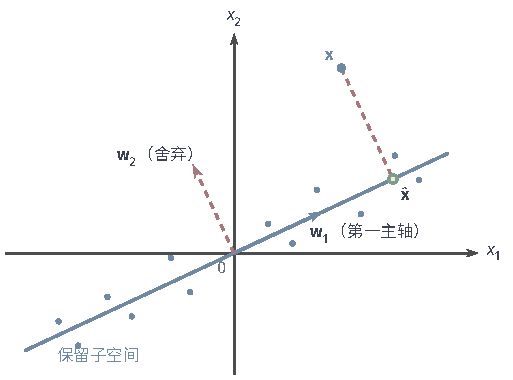
\includegraphics[width=86.935mm]{figures/03-models/01-classic-models/tikz/dim-pca-projection/figure.pdf}
  \caption{二维到一维的正交投影示意。蓝色实线方向$\bm{w}_1$是保留的第一主轴，红色虚线方向$\bm{w}_2$是被舍弃的正交主轴。点$\bm{x}$投到$\widehat{\bm{x}}$，重构残差沿$\bm{w}_2$方向。图中散点为示意位置，未表示真实实验。}
  \label{fig:dim-pca-projection}
\end{figure}

\subsubsection{参数学习}
\label{sec:dim-pca-learning}

最优方向可以通过协方差的谱求出。在单位方向的约束目标中引入乘子$\lambda$，驻点方程为$\bm{S}\bm{w}=\lambda\bm{w}$，投影方差正好等于$\lambda$。按$\lambda_1\geq\cdots\geq\lambda_d\geq0$排序，前$k$个特征向量组成$\bm{V}_k$，其列称为\term{主成分方向}（principal component directions）。取$\bm{W}=\bm{V}_k$得到一个解析最优解；得分$\bm{X}\bm{V}_k$的经验协方差为$\operatorname{diag}(\lambda_1,\ldots,\lambda_k)$，所以这些得分不相关，统计独立还需要额外条件。

方向的唯一性需要分别看基矩阵、子空间与投影算子。一般最优$\bm{W}$是一组正交基，$\operatorname{span}(\bm{W})$是其张成的主子空间，$\bm{P}=\bm{W}\bm{W}^{\top}$是相应投影。若$\lambda_k>\lambda_{k+1}$，主子空间与投影唯一；子空间内部仍可以旋转，任意$k$阶正交矩阵$\bm{Q}$都使$\bm{W}\bm{Q}$给出同一投影，所有最优基可写成$\bm{V}_k\bm{Q}$。

坐标基的旋转却会改变各列及得分之间的关系。从$\bm{W}=\bm{V}_k$出发，若$\bm{Q}$混合不同特征值的方向，$\bm{W}\bm{Q}$的列一般不再是$\bm{S}$的特征向量，得分协方差$\bm{Q}^{\top}\operatorname{diag}(\lambda_1,\ldots,\lambda_k)\bm{Q}$一般也不再对角。因此，互不相关的主成分得分对应排序特征向量基$\bm{V}_k$，而非主子空间中的任意正交基。

如果进一步要求各列为排序后的特征向量，单特征值方向只差符号；所选范围内的重特征值允许在其重特征子空间中旋转。若$\lambda_k=\lambda_{k+1}$，重特征值跨过截断位置，最优主子空间和投影算子也可能不唯一。

实际计算通常对中心化数据作\term{奇异值分解}（singular value decomposition, SVD），写成$\bm{X}=\bm{U}\bm{\Sigma}\bm{V}^{\top}$。右奇异向量给出主方向，$\lambda_j=\sigma_j^2/n$，得分为$\bm{U}_k\bm{\Sigma}_k$。直接SVD无需显式形成$\bm{X}^{\top}\bm{X}$，可以避免条件数平方带来的数值困难。完整稠密分解约需$O(nd\min(n,d))$次运算，只求少数方向时还可使用截断算法；不同实现需要不同的矩阵和计算预算。

当$d\gg n$时，样本空间中的$n\times n$ Gram矩阵$\bm{X}\bm{X}^{\top}$更小。若$\bm{X}\bm{X}^{\top}\bm{u}_j=\sigma_j^2\bm{u}_j$且$\sigma_j>0$，右奇异向量可由$\bm{v}_j=\bm{X}^{\top}\bm{u}_j/\sigma_j$恢复。这仍是同一SVD；第\ref{sec:dim-kpca}节将沿样本空间计算引出核方法。

求出特征值后，可以衡量前$k$个方向保留的方差比例。\term{累计解释方差}（cumulative explained variance）定义为
\begin{equation}
  \eta_k=\frac{\sum_{j=1}^{k}\lambda_j}
                    {\sum_{j=1}^{d}\lambda_j}.
  \label{eq:dim-explained-variance}
\end{equation}
总方差非零时，可以按预先选择的比例确定$k$，也可以查看特征值随序号下降的碎石图。$85\%$、$95\%$等比例是经验阈值，并非预测信息的保证：低方差方向可能包含第\ref{sec:classification-lda-reduction}节的类别判别信息，高方差也可能来自量纲或背景干扰。是否标准化由特征单位和任务决定；服务于预测的维数选择应使用训练集内部的验证结果。

矩阵规模过大时，还可以近似求主子空间。随机化SVD先估计列空间，再分解较小的矩阵；增量PCA按批次更新子空间。二者以近似误差或特定更新规则换取内存与时间收益，评价时需要同时检查求解精度\scite{halko2011}

\subsubsection{理论分析}
\label{sec:dim-pca-theory}

\paragraph{表达能力}
PCA的候选表示由线性子空间限定，适合主要变化集中在该空间附近的数据。弯曲流形的变化可能无法由一个子空间保留，低方差中的任务信息也可能在截断时被删去。方差目标衡量重构中的变化量，预测价值则由具体任务决定。

\paragraph{收敛性}

固定数据上的最优重构可以由Eckart--Young低秩逼近定理说明\scite{eckart1936}下面将这一结果用于PCA的正交重构，再把它与估计总体子空间的问题分开。

在正交投影与平方误差设定下，前$k$维主子空间达到经验全局最优，最小误差等于舍弃特征值的总和。截断处的谱隙进一步决定投影是否唯一：

\begin{theorem}[PCA的最优线性重构性质]
  \label{thm:dim-pca-optimal}
  设$\bm{X}$已中心化，$1\leq k<d$，$\lambda_j$为$\bm{S}=\bm{X}^{\top}\bm{X}/n$按降序排列的特征值。则
  \[
    \min_{\bm{W}^{\top}\bm{W}=\bm{I}_k}
       \frac1n\lVert\bm{X}-\bm{X}\bm{W}\bm{W}^{\top}\rVert_F^2
       =\sum_{j=k+1}^{d}\lambda_j.
  \]
  前$k$个特征向量张成的子空间达到最小值。若$\lambda_k>\lambda_{k+1}$，最优投影算子$\bm{W}\bm{W}^{\top}$唯一，但子空间内的正交基不唯一。
\end{theorem}

\begin{proof}
在所有秩至多为$k$的矩阵中，截断SVD使平方Frobenius误差最小（参见\BookTheoremRef{thm:matrix-analysis-best-low-rank}{第一卷“数学准备”的Eckart--Young--Mirsky定理}）。
截断SVD给出$\bm X\bm V_k\bm V_k^\top$，其平方误差为$\sum_{j>k}\sigma_j^2$；
除以$n$并代入$\lambda_j=\sigma_j^2/n$即得结论。
截断处的严格谱隙使主子空间与投影唯一，唯一的投影仍允许在其子空间中选择不同的正交基。
\end{proof}

迭代谱算法要逼近的是定理中的全局最优投影，可以用特征方程残差和方向正交误差检查数值精度。增加迭代可以改善求解误差；样本是否足以估计总体结构，则是下面的统计问题。

\paragraph{泛化性}

训练样本上的最优平均重构还需要与总体风险比较。设总体中心为$\bm{0}$、协方差为$\bm{\Sigma}_{\star}$，秩$k$正交投影$\bm{P}$的总体重构风险为$R(\bm{P})=\operatorname{tr}((\bm{I}-\bm{P})\bm{\Sigma}_{\star})$。样本风险的最优投影记为$\widehat{\bm{P}}$，总体最优投影记为$\bm{P}_{\star}$；在两者风险差中加入并减去样本协方差项，可以得到
\begin{equation}
  \begin{aligned}
  R(\widehat{\bm{P}})-R(\bm{P}_{\star})
  &\leq\operatorname{tr}
      ((\bm{P}_{\star}-\widehat{\bm{P}})
        (\bm{\Sigma}_{\star}-\bm{S}))\\
  &\leq 2k\lVert\bm{S}-\bm{\Sigma}_{\star}\rVert_2.
  \end{aligned}
  \label{eq:dim-pca-excess-risk}
\end{equation}
第一步由$\widehat{\bm{P}}$的经验最优性得到，第二步使用$\bm{P}_{\star}-\widehat{\bm{P}}$的核范数至多为$2k$；核范数是奇异值之和。若编码使用样本均值，总体风险还要计入均值估计误差。固定$d$、独立同分布且二阶矩有限时，均值与协方差依大数定律收敛，风险差随之趋零。方向估计对谱隙更敏感：相近特征值对应的方向可以明显旋转，重构误差却可能只改变很少。

维数与样本数同步增长时，需要使用相应的高维统计条件。Nadler在尖峰协方差模型中的分析表明，样本特征值和方向可能偏离总体结构，弱信号甚至无法一致识别\scite{nadler2008}Marchenko--Pastur型谱极限提供了一个噪声基准：独立同分布噪声且$d/n$趋于正常数时，即使总体协方差为单位矩阵，样本特征值仍形成非退化的极限谱分布\scite{marchenko1967}该结论依赖具体矩阵模型与比例极限，修正样本谱时也需要这些条件。

高维估计可以利用不同结构限制。稀疏PCA减少活跃载荷，奇异值阈值或收缩则调整谱幅度，例如用于低秩矩阵去噪。Donoho与Gavish的最优硬阈值依赖指定噪声与损失条件，选择修正方式时应先核对其统计模型\scite{donoho2014threshold}

\subsubsection{支持稀疏载荷（Sparse PCA）}
\label{sec:dim-sparse-pca}

主成分若由几乎所有特征组成，很难从载荷看出哪些变量共同驱动一个方向。\term{稀疏PCA}（sparse PCA）限制载荷中的非零项，使一个成分主要由少数变量表达。Zou、Hastie与Tibshirani在2006年用回归式矩阵分解把成分提取与变量选择结合，并讨论基因表达等高维数据\scite{zou2006spca}稀疏要求直接参与优化，而非在普通PCA求解后再删除较小载荷：
\begin{equation}
  \begin{aligned}
  \min_{\bm{A},\bm{B}}\quad&
    \lVert\bm{X}-\bm{X}\bm{B}\bm{A}^{\top}\rVert_F^2
    +\lambda_1\sum_{j=1}^{k}\lVert\bm{b}_j\rVert_1
    +\lambda_2\lVert\bm{B}\rVert_F^2,\\
  \text{约束}\quad&\bm{A}^{\top}\bm{A}=\bm{I}_k.
  \end{aligned}
  \label{eq:dim-sparse-pca}
\end{equation}
在此目标中，$\bm{A},\bm{B}\in\mathbb{R}^{d\times k}$，$\bm{b}_j$是$\bm{B}$第$j$列，$\lambda_1,\lambda_2\geq0$。$\bm{B}$给出编码载荷，$\bm{A}$给出重构方向；$\ell_1$惩罚促使载荷稀疏，平方惩罚缓解相关变量造成的数值不稳定。

交替求解时，固定$\bm{A}$，可以将$\bm{X}$分到$\bm{A}$的列空间与正交补：
\[
  \lVert\bm{X}-\bm{X}\bm{B}\bm{A}^{\top}\rVert_F^2
  =\lVert\bm{X}\bm{A}-\bm{X}\bm{B}\rVert_F^2
   +\lVert\bm{X}(\bm{I}-\bm{A}\bm{A}^{\top})\rVert_F^2.
\]
第二项与$\bm{B}$无关，所以编码载荷可以按列求弹性网回归。转而固定$\bm{B}$，需要最大化$\operatorname{tr}(\bm{A}^{\top}\bm{X}^{\top}\bm{X}\bm{B})$，这是寻找最佳正交对齐的Procrustes问题，可由SVD求解。交替更新通常得到局部解，初始化与惩罚强度的敏感性需要检查。

稀疏载荷让变量组合更容易辨认，同时也改变了得分之间的关系。$\bm{B}$各列通常不正交，得分方差可能重叠，因此各成分方差之和不能直接作为标准PCA式的解释方差。基因表达和文本等应用需要同时评价稀疏程度、重构效果与跨样本稳定性。

\subsubsection{支持异常值与低秩加稀疏分解（Robust PCA）}
\label{sec:dim-robust-pca}

稀疏PCA限制使用的变量，异常值处理则需要改变误差模型。幅度很大的污染会在平方误差中占据较大权重；固定摄像机视频的低变化背景与少数变化像素提供了一个例子。把视频帧排为观测矩阵$\bm{M}\in\mathbb{R}^{n\times d}$，可尝试分解成低秩背景$\bm{L}$与稀疏扰动$\bm{E}$。这里的\term{鲁棒PCA}（robust PCA, RPCA）专指低秩加稀疏分解，稳健子空间估计还包括其他污染设定。

同时寻找低秩部分和稀疏部分时，直接最小化$\operatorname{rank}(\bm{L})+\lambda\lVert\bm{E}\rVert_0$存在组合困难。\term{主成分追踪}（principal component pursuit, PCP）用两个凸惩罚替代秩和非零元素数：
\begin{equation}
  \min_{\bm{L},\bm{E}}\
     \lVert\bm{L}\rVert_*+\lambda\lVert\bm{E}\rVert_1,
  \qquad \bm{M}=\bm{L}+\bm{E}.
  \label{eq:dim-pcp}
\end{equation}
核范数$\lVert\bm{L}\rVert_*=\sum_j\sigma_j(\bm{L})$鼓励较少的非零奇异值；$\lVert\bm{E}\rVert_1$为所有元素绝对值之和，鼓励较少的非零污染项。两个惩罚分别作用于整体秩结构与逐元素扰动。

分解能否恢复真实两部分，关键在于它们是否可区分。一个既低秩又稀疏的矩阵可以在$\bm{L}$与$\bm{E}$之间转移，造成歧义。Candès等的精确恢复定理要求低秩部分不相干，即奇异向量不集中在少数坐标，还限制秩、污染比例与随机支持。在这些条件下，$\lambda=1/\sqrt{\max(n,d)}$无需预先知道污染幅度；任意位置的对抗污染仍需另查是否符合条件\scite{candes2011rpca}

两个惩罚可以由\term{交替方向乘子法}（alternating direction method of multipliers, ADMM）分开求解，再通过重构约束协调。取惩罚参数$\rho>0$，引入与$\bm{M}$同形的$\bm{U}$作为缩放对偶变量，即拉格朗日乘子除以$\rho$。固定$\bm{U}$并略去无关常数，增广目标为
\[
  \lVert\bm{L}\rVert_*+\lambda\lVert\bm{E}\rVert_1
  +\frac{\rho}{2}
   \lVert\bm{M}-\bm{L}-\bm{E}+\bm{U}\rVert_F^2.
\]
固定$\bm{E}$更新$\bm{L}$，再用新$\bm{L}$更新$\bm{E}$，分别对应两种阈值运算。随后将尚未满足的重构误差加到$\bm{U}$，让下一轮继续校正约束偏差。从$\bm{U}^{(0)}=\bm{0}$开始时，一轮更新为
\begin{equation}
  \begin{aligned}
  \bm{L}^{(t+1)}&=\operatorname{SVT}_{1/\rho}
                  (\bm{M}-\bm{E}^{(t)}+\bm{U}^{(t)}),\\
  \bm{E}^{(t+1)}&=\mathcal{S}_{\lambda/\rho}
                  (\bm{M}-\bm{L}^{(t+1)}+\bm{U}^{(t)}),\\
  \bm{U}^{(t+1)}&=\bm{U}^{(t)}
                   +\bm{M}-\bm{L}^{(t+1)}-\bm{E}^{(t+1)}.
  \end{aligned}
  \label{eq:dim-rpca-admm}
\end{equation}
逐元素软阈值为$\mathcal{S}_{a}(u)=\operatorname{sign}(u)(|u|-a)_+$，$\operatorname{SVT}_{a}$则将同一运算作用于奇异值。模型中的$\bm{E}$代表稀疏扰动，迭代中的$\bm{U}$累积重构约束误差。为检查固定$\rho$下的停止条件，需要同时计算
\[
  \begin{aligned}
    r_{\mathrm{pri}}^{(t+1)}
      &=\lVert\bm{M}-\bm{L}^{(t+1)}-\bm{E}^{(t+1)}\rVert_F,\\
    r_{\mathrm{dual}}^{(t+1)}
      &=\rho\lVert\bm{E}^{(t+1)}-\bm{E}^{(t)}\rVert_F.
  \end{aligned}
\]
原始残差检查重构等式，对偶残差检查第二个子问题的变化是否仍破坏前一个子问题的平衡。两项均应低于按数据尺度设置的容差；迭代次数只是预算，不能代替这两项检查。

小幅稠密噪声可通过$\lVert\bm{M}-\bm{L}-\bm{E}\rVert_F\leq\delta$的稳定PCP约束容纳。在线变体处理流式观测，侧信息变体利用已知子空间特征。视频背景、遮挡或异常检测中的污染需要与所选模型对应；例如整行异常更适合组稀疏惩罚，逐元素稀疏并不描述同一种结构。

\subsubsection{小结}
\label{sec:dim-pca-summary}

PCA在给定数据上得到平均平方误差最小的正交线性压缩，并提供共享的编码与重构。所得子空间受维数、尺度和异常值影响，总体估计又受样本量与谱隙影响。稀疏PCA约束载荷，RPCA描述污染，第\ref{sec:dim-ppca}节的概率PCA描述噪声与潜变量；这些扩展需要按各自改变的假设选择。

\subsection{典型相关分析（CCA）}
\label{sec:dim-cca}

一张图像和对应文字使用不同坐标，却可以描述共同内容。分别保留两侧最大方差，可能先保留各自独有的变化。\term{典型相关分析}（canonical correlation analysis, CCA）让成对观测分别投影，再选择对应得分相关系数最大的方向，从而提取共同变化。Hotelling的经典工作建立了这一双视图分析框架\scite{hotelling1936cca}

\subsubsection{模型结构}
\label{sec:dim-cca-structure}

将成对观测中心化，记$\bm{x}\in\mathbb{R}^{d_x}$、$\bm{y}\in\mathbb{R}^{d_y}$，两侧协方差为$\bm{\Sigma}_{xx}$、$\bm{\Sigma}_{yy}$，交叉协方差为$\bm{\Sigma}_{xy}=\mathbb{E}[\bm{x}\bm{y}^{\top}]$。用同一批配对样本估计这些矩阵后，第一对方向按投影相关系数选择：
\begin{equation}
  \max_{\bm{w}_x,\bm{w}_y}
  \frac{\bm{w}_x^{\top}\bm{\Sigma}_{xy}\bm{w}_y}
  {\sqrt{\bm{w}_x^{\top}\bm{\Sigma}_{xx}\bm{w}_x}
   \sqrt{\bm{w}_y^{\top}\bm{\Sigma}_{yy}\bm{w}_y}}.
  \label{eq:dim-cca-correlation}
\end{equation}
相关系数只有在两侧投影方差均非零时有定义。缩放方向不改变相关性，因此可以令两侧方差均为$1$，将求解转为最大化交叉协方差。

图\ref{fig:dim-cca-shared}用两个视图比较方差与共有信息。各自方差最大的坐标$u$、$v$相互独立，较小方差的坐标却同为$t$，所以PCA与CCA会选择不同方向。此比较保留原坐标的方差；逐坐标标准化改变方差结构，也会改变PCA选择。

\begin{figure*}[!ht]
  \centering
  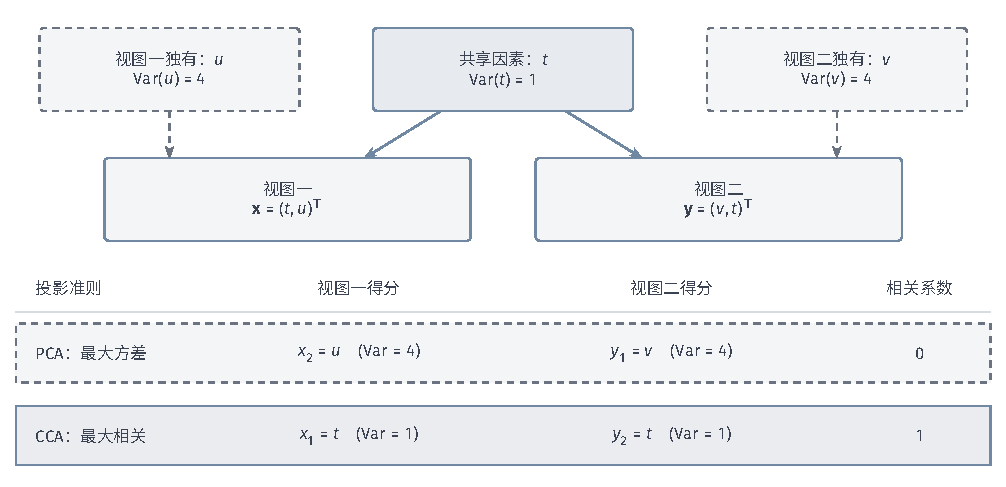
\includegraphics[width=169.000mm]{figures/03-models/01-classic-models/tikz/dim-cca-shared/figure.pdf}
  \caption{CCA提取共有变化的构造例子。设$t,u,v$相互独立且均值为零，方差依次为$1,4,4$；两视图为$\bm{x}=(t,u)^\top$和$\bm{y}=(v,t)^\top$。实线连接共享因素，虚线连接各视图独有因素。各保留一维时，PCA选择$u,v$，CCA选择$t,t$，对应相关系数分别为$0$和$1$。箭头表示坐标构造关系，图中结论针对给定总体，不是样本拟合结果。}
  \label{fig:dim-cca-shared}
\end{figure*}

提取多对得分时，要求同一视图内$\bm{W}_x^{\top}\bm{\Sigma}_{xx}\bm{W}_x=\bm{I}_k$、$\bm{W}_y^{\top}\bm{\Sigma}_{yy}\bm{W}_y=\bm{I}_k$，使各得分方差为一且互不相关。这是协方差度量下的正交，原坐标中的方向未必欧氏正交。跨视图得分协方差可对角化为$\operatorname{diag}(\rho_1,\ldots,\rho_k)$，可识别的方向对数则同时受维数、样本秩与交叉协方差秩限制。

\subsubsection{参数学习}
\label{sec:dim-cca-learning}

两侧协方差正定时，可以先白化，使每侧协方差变成单位阵。白化后的交叉协方差及其SVD为
\[
  \bm{K}=\bm{\Sigma}_{xx}^{-1/2}
               \bm{\Sigma}_{xy}\bm{\Sigma}_{yy}^{-1/2},
  \qquad
  \bm{K}=\bm{U}\bm{D}\bm{V}^{\top}.
\]
令$\bm{a}=\bm{\Sigma}_{xx}^{1/2}\bm{w}_x$、$\bm{b}=\bm{\Sigma}_{yy}^{1/2}\bm{w}_y$，方差约束成为单位范数约束，目标成为$\max\bm{a}^{\top}\bm{K}\bm{b}$。取$\bm{K}$的首对左右奇异向量，就达到最大奇异值；多对方向由相应奇异向量依次取得：
\begin{equation}
  \bm{W}_x=\bm{\Sigma}_{xx}^{-1/2}\bm{U}_k,\qquad
  \bm{W}_y=\bm{\Sigma}_{yy}^{-1/2}\bm{V}_k,
  \label{eq:dim-cca-svd}
\end{equation}
$\bm{D}$的前$k$个对角元给出典型相关系数。实现白化时，可以使用Cholesky分解和三角求解，避免显式形成逆矩阵。

这一求解也可写成广义特征值问题。约束驻点满足$\bm{\Sigma}_{xy}\bm{w}_y=\rho\bm{\Sigma}_{xx}\bm{w}_x$及另一侧的对称方程，消去$\bm{w}_y$后得到
\[
  \bm{\Sigma}_{xy}\bm{\Sigma}_{yy}^{-1}
       \bm{\Sigma}_{yx}\bm{w}_x
  =\rho^2\bm{\Sigma}_{xx}\bm{w}_x.
\]
样本协方差奇异时，可只在非零方差子空间中求解，或分别加$\lambda_x\bm{I}$、$\lambda_y\bm{I}$进行正则化。正则化改变了归一化度量，训练相关系数因而需要配合留出配对样本的相关性一起评价。

共有变化也可以在非线性特征中寻找。核CCA固定核映射后匹配相关性，深度CCA则直接学习两侧变换\scite{andrew2013dcca}Andrew等2013年的方法通过两条联合训练的参数映射保留相关性目标，让新样本以前向计算获得表示。这改变了固定核的表示限制与样本展开方式，同时增加了需要控制的模型复杂度。

\subsubsection{小结}
\label{sec:dim-cca-summary}

CCA以共有线性变化组织配对传感器、多模态匹配或跨域表示，目标是相关性。某一视图独有却重要的信息可能未被保留，相关性也需要额外假设才能作因果解释。高维小样本容易高估训练相关性，应通过正则化与样本外配对检验控制这一问题。双塔表示和对比学习也对齐多视图，但各自的负采样、损失与训练规则需要另外说明。

\subsection{独立成分分析（ICA）}
\label{sec:dim-ica}

协方差为零只能排除线性相关。例如$X\sim\mathcal{N}(0,1)$时，$X$与$X^2$的协方差为零，后者却完全由前者确定。混合的多个源信号若要彼此分离，需要进一步利用分布中的依赖。\term{独立成分分析}（independent component analysis, ICA）据此结合源独立性与非高斯结构估计混合过程，用于说话人分离、脑电活动分析和眼动伪迹分离等任务\scite{comon1994ica}

信息论提供了另一种减少分量依赖的准则。Bell与Sejnowski在1995年研究非线性网络中的信息传递，推导出利用协方差以外统计信息的学习规则，并讨论未知混合语音的分离和未知回声的消除\scite{bell1995infomax}这类问题称为盲信号处理，因为混合或传播过程未知；对源信号的结构仍需作出假设。

\subsubsection{模型结构}
\label{sec:dim-ica-structure}

为说明解混关系，先取中心化、无噪声且源数等于观测通道数的模型：
\begin{equation}
  \bm{x}=\bm{A}\bm{s},\qquad
  \bm{z}=\bm{W}^{\top}\bm{x},\qquad
  \bm{W}^{\top}=\bm{A}^{-1}.
  \label{eq:dim-ica-model}
\end{equation}
混合矩阵$\bm{A}\in\mathbb{R}^{d\times d}$可逆，源$\bm{s}$的分量相互独立。此处$\bm{W}$的列存放解混方向，所以$\bm{W}=\bm{A}^{-\top}$。若将$\bm{A}^{-1}$直接称为解混矩阵，则编码用它左乘观测；两种记法描述同一运算。

识别这些方向还要求源非退化，且至多一个源为高斯。多个标准高斯源的联合分布在正交旋转后相同，因而无法从观测辨认该子空间中的方向。源排列与尺度也存在歧义：交换源及混合列，或对两者作反向缩放，观测$\bm{x}$保持相同。

存在密度时，可以比较解混分量的联合分布与边际乘积，用KL散度衡量剩余依赖。写成熵的形式为
\[
  I(z_1,\ldots,z_d)
  =\sum_{j=1}^{d}h(z_j)-h(\bm{z}),
\]
$h$为微分熵，上式要求各项有定义；散度为零恰好对应分量独立。也可以在单位方差约束下寻找非高斯方向，例如最大化负熵$J(z)=h(g)-h(z)$，其中$g$与$z$均值、方差相同且服从高斯分布。独立量相加趋向高斯提供了分离的直觉，具体对比量在有限线性组合中的性质仍需检验，不能直接由中心极限定理得到严格单调性。

指定各源密度$p_j$后，还可以按观测似然估计解混方向。变量替换同时改变密度和体积，得到
\begin{equation}
  \ell(\bm{W})
  =n\log|\det\bm{W}|
   +\sum_{i=1}^{n}\sum_{j=1}^{d}
        \log p_j(\bm{w}_j^{\top}\bm{x}_i).
  \label{eq:dim-ica-likelihood}
\end{equation}
行列式项是解混Jacobian对体积的校正。互信息、非高斯性与似然从不同角度利用分布信息；近似对比函数或错误源密度会改变目标，得到的方向也可能不同。

\subsubsection{参数学习}
\label{sec:dim-ica-learning}

求独立方向之前，通常先去除协方差中的尺度和相关性。\term{白化}（whitening）将协方差变成单位阵：若$\bm{S}=\bm{V}\bm{\Lambda}\bm{V}^{\top}$且保留特征值为正，取$\widetilde{\bm{x}}=\bm{\Lambda}^{-1/2}\bm{V}^{\top}\bm{x}$。源方差规范为$1$后，白化空间中的混合矩阵正交，剩下的是方向选择。

图\ref{fig:dim-ica-whitening}给出白化仍未分离源的例子。左图协方差已为单位阵，但$x_1$接近边缘时，$x_2$允许的区间随之改变，两个分量仍依赖。旋转到右图源坐标后，均匀方形的联合分布才分成两个一维均匀分布。旋转前后的协方差相同，需要更完整的分布信息选择方向。

\begin{figure}[!ht]
  \centering
  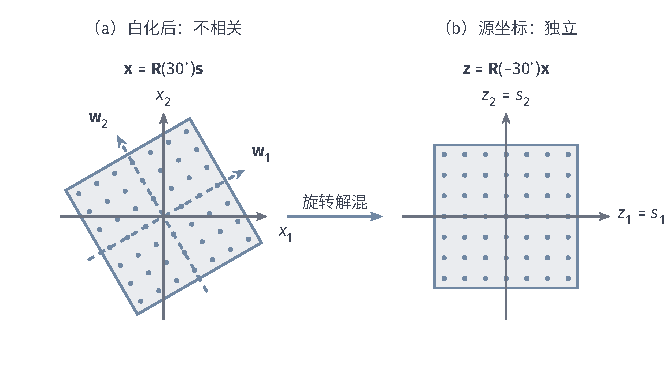
\includegraphics[width=112.000mm]{figures/03-models/01-classic-models/tikz/dim-ica-whitening/figure.pdf}
  \caption{白化与独立源恢复的区别。设$s_1,s_2$独立且均服从$\mathcal{U}[-\sqrt3,\sqrt3]$，$\bm{R}(\theta)$为逆时针旋转矩阵。左图为$\bm{x}=\bm{R}(30^\circ)\bm{s}$，右图为逆旋转恢复的$\bm{s}$；两者协方差均为$\bm{I}_2$，只有右侧所示坐标对应独立源。实线轮廓为总体支持域，圆点为确定性格点，虚线箭头为解混方向。图为无量纲构造示意，未运行ICA优化；该方形解混本身不减少维数。}
  \label{fig:dim-ica-whitening}
\end{figure}

FastICA用光滑非二次函数$G$构造非高斯性对比量。单位方向$\bm{u}$在白化数据上产生方差为$1$的投影$\bm{u}^{\top}\widetilde{\bm{x}}$，可以将其与标准高斯变量$\nu$比较：
\begin{equation}
  J_G(\bm{u})
  =\left[
    \mathbb{E}G(\bm{u}^{\top}\widetilde{\bm{x}})
    -\mathbb{E}G(\nu)
  \right]^2,
  \qquad \lVert\bm{u}\rVert_2=1.
  \label{eq:dim-fastica-contrast}
\end{equation}
该目标近似前述负熵，其性质取决于$G$的选择。令$g=G'$；括号内的差非零、且期望与微分可交换时，$J_G$的球面驻点满足$\mathbb{E}G(\bm{u}^{\top}\widetilde{\bm{x}})$的约束驻点方程
\[
  \bm{a}(\bm{u})
  :=\mathbb{E}\!\left[\widetilde{\bm{x}}
       g(\bm{u}^{\top}\widetilde{\bm{x}})\right]
  =\beta\bm{u},
  \qquad
  \beta=\bm{u}^{\top}\bm{a}(\bm{u}).
\]
乘子$\beta$对应单位范数约束。近似求解时，在当前点固定$\beta$，并将Jacobian中的
$\mathbb{E}[\widetilde{\bm{x}}\widetilde{\bm{x}}^{\top}
g'(\bm{u}^{\top}\widetilde{\bm{x}})]$
近似为$c\bm{I}$，其中$c=\mathbb{E}g'(\bm{u}^{\top}\widetilde{\bm{x}})$。白化给出单位协方差，加上$g'$权重后的矩阵仍需这一步近似。若$c-\beta\ne0$，近似Newton步为
\[
  \bm{u}-\frac{\bm{a}(\bm{u})-\beta\bm{u}}{c-\beta}
  =\frac{c\bm{u}-\bm{a}(\bm{u})}{c-\beta}.
\]
方向可作符号翻转，归一化又消去非零标量，所以更新可直接使用$\bm{a}(\bm{u})-c\bm{u}$。将期望换成样本平均，从当前单位方向$\bm{u}^{(t)}$出发，就得到FastICA固定点更新：
\begin{equation}
  \begin{aligned}
  \bm{v}^{(t+1)}
    &=\frac1n\sum_{i=1}^{n}
      \widetilde{\bm{x}}_i
           g((\bm{u}^{(t)})^{\top}\widetilde{\bm{x}}_i)\\
    &\quad-\left[\frac1n\sum_{i=1}^{n}
      g'((\bm{u}^{(t)})^{\top}\widetilde{\bm{x}}_i)\right]\bm{u}^{(t)},\\
  \bm{u}^{(t+1)}
    &=\bm{v}^{(t+1)}/\lVert\bm{v}^{(t+1)}\rVert_2.
  \end{aligned}
  \label{eq:dim-fastica}
\end{equation}
常用$G(u)=\log\cosh u$或$G(u)=u^4/4$，对应$g(u)=\tanh u$和$g(u)=u^3$；后者的四次矩对极端值更敏感。多个成分可逐个与已求方向正交化，也可整组对称正交化。停止时检查方向变化，并把符号翻转计为同一方向\scite{hyvarinen1999fastica}

FastICA的收敛速度取决于源分布、对比函数与初始化，更新向量接近零时需重新初始化或调整设置。Infomax按输出非线性最大化输出熵，采用梯度更新；JADE通过联合对角化四阶累积量矩阵使用高阶统计信息。比较这些算法的成本，需要同时计入每次更新所用的信息与运算。

\subsubsection{小结}
\label{sec:dim-ica-summary}

ICA从去相关转向独立源识别，依赖源独立、非高斯与可识别性条件。标准方形ICA仍输出原维数；先截断白化空间，或取源数少于通道数的模型，才同时压缩。源数多于通道数时是欠定混合，通常需要稀疏等额外结构；非线性混合、相关源、多个高斯源及强噪声也需要不同的识别条件与算法。

\subsection{非负矩阵分解（NMF）}
\label{sec:dim-nmf}

词频、光谱强度与像素亮度为非负量，可以尝试将观测解释成多个成分的相加。\term{非负矩阵分解}（nonnegative matrix factorization, NMF）要求基与系数都非负，使每个成分增加重构值，而不通过正负抵消参与表示。

% 为两条完整的历史文献边注保留空间。
\Needspace{12\baselineskip}
非负结构可以与不同的误差模型配合。Paatero与Tapper在1994年根据环境测量误差加权残差，并在正矩阵分解中施加非负约束\scite{paatero1994nmf}Lee与Seung在1999年用人脸和文本说明加性表示如何形成组成成分\scite{lee1999nmf}两项工作分别强调测量约束与部件表示，损失及应用假设也随所解释的对象而变。

\subsubsection{模型结构}
\label{sec:dim-nmf-structure}

将非负观测排成$\bm{X}\in\mathbb{R}_{+}^{n\times d}$，寻找较少的共享基及各样本的非负系数：
\begin{equation}
  \bm{X}\approx\bm{W}\bm{H},\qquad
  \bm{W}\in\mathbb{R}_{+}^{n\times k},\quad
  \bm{H}\in\mathbb{R}_{+}^{k\times d}.
  \label{eq:dim-nmf-factorization}
\end{equation}
此处$\bm{W}$存放样本系数，与PCA的正交基约定不同；第$i$行是样本$i$的表示，$\bm{H}$各行是共享基。文档可由主题词模式相加，光谱可由成分谱相加。非负约束规定这种加性关系，基是否局部化、系数是否稀疏以及主题是否可读，则需要数据与额外约束支持。

图\ref{fig:dim-nmf-parts}用固定的横条与竖条基演示加性重构。九个像素按行展开后，$\bm{H}$的两行为基的转置，系数$(0.6,1.0)$给出右侧图案。中心像素同时获得两项贡献，值为$1.6$。这一固定字典下，两系数足以描述该图案；压缩成本还需计入字典，一般观测也可能存在重构误差。

\begin{figure}[htbp]
  \centering
  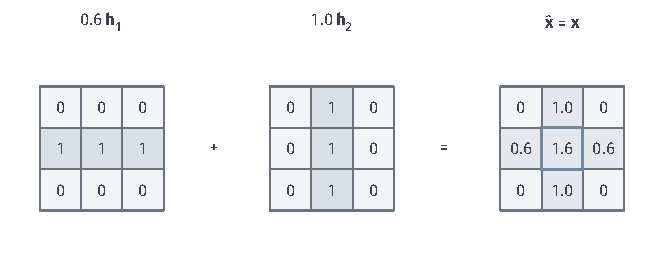
\includegraphics[width=112.000mm]{figures/03-models/01-classic-models/tikz/dim-nmf-parts/figure.pdf}
  \caption{两个非负基的加性重构。左侧两幅$3\times3$栅格分别给出未加权的横条、竖条基，外侧系数为$0.6$与$1.0$；右侧为逐像素加权和，粗框中心格等于$0.6+1.0=1.6$。数值无量纲，本构造恰好精确重构，不表示NMF总能学出这样的部件或保证唯一分解。}
  \label{fig:dim-nmf-parts}
\end{figure}

观测类型决定怎样衡量重构误差。连续观测常用$\frac12\lVert\bm{X}-\bm{W}\bm{H}\rVert_F^2$，对应固定方差高斯残差的似然；非负计数可以使用广义KL散度，也称I散度：
\begin{equation}
  \mathcal{L}_{\mathrm{KL}}
  =\sum_{i,j}\left[
      \bm{X}_{i,j}\log\frac{\bm{X}_{i,j}}{(\bm{W}\bm{H})_{i,j}}
      -\bm{X}_{i,j}+(\bm{W}\bm{H})_{i,j}\right].
  \label{eq:dim-nmf-kl}
\end{equation}
计算采用$0\log(0/u)=0$；观测$\bm{X}_{i,j}>0$而重构为零时，损失为无穷大。条件独立Poisson计数的负对数似然与上式只差数据常数；存在过度离散时，则需要调整观测模型。

NMF的分解具有尺度和排列自由度。对正对角矩阵$\bm{D}$，$\bm{W}\bm{H}=(\bm{W}\bm{D})(\bm{D}^{-1}\bm{H})$，同时交换基与对应系数也保持重构。稀疏、平滑和归一化可以减少部分歧义，唯一性仍需相应识别条件。

\subsubsection{参数学习}
\label{sec:dim-nmf-learning}

基与系数的联合优化非凸，固定一侧后，平方误差子问题则是非负约束凸问题。Lee与Seung的乘法更新用非负比率维持可行性；下面的乘除均逐元素计算，两侧按顺序更新\scite{lee2001nmf}
\begin{equation}
  \begin{aligned}
    \bm{W}&\leftarrow\bm{W}\odot
       \frac{\bm{X}\bm{H}^{\top}}
        {\bm{W}\bm{H}\bm{H}^{\top}},\\
    \bm{H}&\leftarrow\bm{H}\odot
       \frac{\bm{W}^{\top}\bm{X}}
        {\bm{W}^{\top}\bm{W}\bm{H}}.
  \end{aligned}
  \label{eq:dim-nmf-mu}
\end{equation}
正初始化且更新有定义时，辅助函数可以证明目标不增加；结合非负下界，目标值序列便收敛。参数是否到达驻点或极小值还需进一步条件。零元素可能被锁定，因此实现还要处理零分母、检查约束梯度残差，并比较多次初始化结果。

其他求解方式可以更直接地检查约束残差。投影梯度用$\max(0,\cdot)$返回非负区域，交替非负最小二乘更充分地求各子问题；HALS和坐标下降逐个更新基或系数，可以利用稀疏结构。达到给定精度的速度取决于损失、稀疏性和初始化，目标单调性只说明下降性质\scite{lin2007nmf}

固定$\bm{H}$后，新样本通过非负最小二乘或相应KL目标编码。平方误差下求$\min_{\bm{w}\geq0}\lVert\bm{x}-\bm{H}^{\top}\bm{w}\rVert_2^2$，需要求系数，而非复用一个线性投影。稠密平方误差更新的主要乘法约需$O(ndk)$，训练总成本还取决于迭代次数。

\subsubsection{小结}
\label{sec:dim-nmf-summary}

NMF以加性成分解释非负数据，求解和使用需要考虑非凸目标及表示歧义。低秩PCA与NMF一般都存在重构误差，压缩是否足够精确要由所保留成分决定。中心化后的负值若通过平移变成非负，也会改变加性分解的含义，需要由任务支持这一预处理。

在相应归一化与计数似然约定下，式\eqref{eq:dim-nmf-kl}的NMF与概率隐语义索引具有同一目标，更新算法则不同\scite{ding2008nmf-plsi}潜在狄利克雷分配还为文档主题比例设置先验\scite{blei2003}更多约束可分别用于多轴数据、基的构成、成分关系、稀疏结构和层次组织，对应非负张量分解、凸NMF、正交NMF、稀疏NMF及深度NMF。采用哪些约束，应依据实际成分需要具有什么含义。

\subsection{稀疏编码与字典学习}
\label{sec:dim-sparse-coding}

一个图像块可能仅包含几条边缘，却要从许多位置和方向选择它们。可以准备较大的基向量库，让每个样本只激活少数基。\term{稀疏编码}（sparse coding）在固定字典中求这些活跃系数，\term{字典学习}（dictionary learning）进一步从数据学习共享的基。

Olshausen与Field在1996年研究自然图像的统计规律是否能解释初级视觉皮层响应的局部性、方向选择性与空间频率选择性。他们用稀疏线性编码学习具有这些性质的基，并与小波表示比较\scite{olshausen1996}这给视觉神经科学和信号表示建立了联系；感受野外观相似的证据，仍不足以确定生物学习过程与该算法相同。

\subsubsection{模型结构}
\label{sec:dim-sparse-coding-structure}

把共享基作为$\bm{D}\in\mathbb{R}^{d\times p}$的列，称$\bm{d}_j$为字典原子，$p$为原子数。允许$p>d$时，字典称为过完备。样本由$\bm{x}_i\approx\bm{D}\bm{\alpha}_i$重构，$\bm{\alpha}_i\in\mathbb{R}^{p}$只激活少数坐标。取$\lambda>0$控制稀疏惩罚的强度，通过误差与惩罚的加权和选择字典和系数：
\begin{equation}
  \begin{aligned}
  \min_{\bm{D},\{\bm{\alpha}_i\}}\quad&
   \sum_{i=1}^{n}\left[
      \tfrac12\lVert\bm{x}_i-\bm{D}\bm{\alpha}_i\rVert_2^2
      +\lambda\lVert\bm{\alpha}_i\rVert_1\right],\\
  \text{约束}\quad&\lVert\bm{d}_j\rVert_2\leq1
                 \quad(j=1,\ldots,p).
  \end{aligned}
  \label{eq:dim-dictionary-objective}
\end{equation}
若字典无限放大、系数相应缩小，重构不变而$\ell_1$惩罚降低；列范数约束排除了这种尺度退化。此模型允许正负系数和非正交基，表示长度甚至可以超过原维数，与NMF的非负及PCA的正交约束不同。

只使用一个含$s$个原子的支持集时，重构落在至多$s$维的线性子空间；更换活跃原子，就切换到其他子空间。稀疏表示因而可以用多个子空间组织不同样本，而非要求它们都位于同一光滑低维流形。活跃集合随输入改变，编码通常也是非线性的。

\subsubsection{参数学习}
\label{sec:dim-sparse-coding-learning}

给定字典后，每个样本独立求Lasso型系数，可用坐标下降、LARS或近端梯度。对一个样本，取$L\geq\lVert\bm{D}^{\top}\bm{D}\rVert_2$且$L>0$，ISTA把重构误差的梯度步与稀疏惩罚结合：
\begin{equation}
  \bm{\alpha}^{(t+1)}
  =\mathcal{S}_{\lambda/L}\left(
      \bm{\alpha}^{(t)}
      +L^{-1}\bm{D}^{\top}
          (\bm{x}-\bm{D}\bm{\alpha}^{(t)})\right).
  \label{eq:dim-ista}
\end{equation}
该更新先沿重构误差的负梯度移动，再作$\ell_1$惩罚的软阈值近端映射。FISTA增加外推，在固定字典的凸子问题条件下改善目标值收敛率；字典与系数联合学习仍需单独分析\scite{beck2009fista}

给定编码，记$\bm{A}=[\bm{\alpha}_1,\ldots,\bm{\alpha}_n]\in\mathbb{R}^{p\times n}$，字典步最小化$\frac12\lVert\bm{X}^{\top}-\bm{D}\bm{A}\rVert_F^2$并满足列范数约束。MOD用无约束解$\bm{X}^{\top}\bm{A}^{\dagger}$更新方向，常见实现再归一化各列。各字典列共同影响重构残差，无约束解后逐列归一化一般不能得到列范数约束下的精确解。需要严格下降时，应采用适当的约束求解或验证更新。

K-SVD通常采用$\lVert\bm{\alpha}_i\rVert_0\leq s$的活跃原子数约束。更新一个原子时，先去掉其他原子的重构，只保留使用该原子的样本，再用残差的秩一SVD同时更新原子与活跃系数。该求解配合的是非零项数约束，与式\eqref{eq:dim-dictionary-objective}的$\ell_1$目标不同\scite{aharon2006ksvd}

在线字典学习按小批样本更新，积累编码二阶统计量及观测交叉统计量以近似求字典，减少反复扫描全数据的开销。总成本还取决于原子数、每个稀疏子问题的精度和更新次数，一次遍历不能确定达到指定精度的完整成本\scite{mairal2009online}

\subsubsection{小结}
\label{sec:dim-sparse-coding-summary}

少量活跃原子可以组合出多种信号，适合去噪、修复和可组合模式的表示。新样本仍需求系数，因此使用时需要优化预算。压缩感知进一步研究从少量线性测量恢复稀疏信号，恢复条件还涉及测量矩阵的受限等距等性质。

字典和活跃约束可以随任务扩展：判别式字典利用标签，结构稀疏规定原子共同出现的方式，卷积稀疏编码在位置间共享滤波器。稀疏自编码器和层次表示也使用类似约束，算法与理论是否相通仍需比较目标和更新。本章讨论稀疏编码，是因为它以少数线性成分描述样本，而非因为编码向量一定更短。

\subsection{随机投影（Random Projection）}
\label{sec:dim-rp}

前述投影和字典都先从数据学习。流式数据维数很高时，也可以问：预先固定一个映射，是否仍能近似保留点间欧氏距离？\term{随机投影}（random projection）按指定分布抽取矩阵，再统一变换全部样本。Johnson--Lindenstrauss引理给出这种构造的保距依据，保证针对抽取映射前固定的有限点集，以较高概率同时成立\scite{johnson1984jl}

实现这种映射还要考虑生成和计算成本。Achlioptas于2003年构造离散随机矩阵，让投影由属性的加减、聚合和统一缩放实现\scite{achlioptas2003}其变化在于算术操作，有限点集上的几何保证仍不依赖先拟合数据。

\subsubsection{模型结构}
\label{sec:dim-rp-structure}

用$\bm{\Pi}\in\mathbb{R}^{k\times d}$编码$\bm{z}=\bm{\Pi}\bm{x}$。独立高斯元素$\bm{\Pi}_{i,j}\sim\mathcal{N}(0,1/k)$给出最直接的构造：对固定$\bm{x}$，平方范数的平均值为
\[
  \mathbb{E}_{\bm{\Pi}}\lVert\bm{\Pi}\bm{x}\rVert_2^2
  =\lVert\bm{x}\rVert_2^2.
\]
该期望只说明平均保范数。一次采样要同时服务整批样本，还需控制偏离均值的尾概率，再让各点对的误差同时受限。

稀疏矩阵进一步减少乘法和存储。Achlioptas的元素以$1/6$概率取$\sqrt{3/k}$、以$1/6$概率取$-\sqrt{3/k}$，其余取零，也可建立集中界。Li、Hastie与Church研究更稀疏的构造时，还需考虑输入分量的集中程度；二阶矩相同并不足以支持任意稀疏率下的同一误差界\scite{li2006sparserp}

快速Johnson--Lindenstrauss变换用随机符号、Hadamard变换及后续抽样或稀疏映射组织计算。结构化变换部分约为$O(d\log d)$，总成本还包括输出维数和精度相关项。与直接存储$kd$个高斯元素相比，它对内存、算术和输入尺寸有不同要求\scite{ailon2009fjlt}

\subsubsection{参数学习}
\label{sec:dim-rp-learning}

随机投影直接生成映射，需要选择的是$k$、矩阵分布和稀疏程度。训练与新样本使用相同矩阵，稠密编码每样本约需$O(kd)$次运算。分布式环境若用共同种子复现映射，还要固定伪随机数实现和矩阵元素的生成顺序。

输出维数决定误差、点数和失败概率之间的取舍。下面的充分条件往往保守，给出的$k$若已超过$d$，就没有实际压缩收益。可以在训练或验证数据上测量距离失真，比较较小维数，或先随机压缩到中等维数再做PCA、最近邻搜索；下游结果则按任务另行评价。

对映射抽取前固定的有限点集，高斯随机投影给出同时保留平方距离的充分维数条件，可用来设置候选$k$（参见\BookTheoremRef{thm:probability-johnson-lindenstrauss}{第一卷“数学准备”的“高斯随机投影的距离保持”定理}）。观察映射后，从这批固定点中选择要比较的点对，仍被同时保距事件覆盖；观察映射后再构造点集之外的新查询，则超出这里的固定点集保证。

\subsubsection{理论分析}
\label{sec:dim-rp-theory}

\paragraph{表达能力}
随机投影用线性映射近似保留指定点集的距离，输出维数限定能保留的信息。它没有从样本学习非线性流形，有限点集的保距也没有为完整分布建立可逆表示。

要用一次采样同时服务全部点对，需要让维数足以控制整批失败概率。给定点数、相对误差和失败概率后，可使用以下充分条件。

对$n\geq2$个预先固定的点，取$0<\varepsilon,\delta<1$。
上述定理给出充分条件
\[
  k\geq\frac{8}{\varepsilon^2}\log\frac{n(n-1)}{\delta},
\]
使同一高斯投影以至少$1-\delta$的概率同时把全部点对的平方距离保持在原值的
$1\pm\varepsilon$倍内。这里$\delta$控制整批点对的失败概率，不是每一对单独的失败概率。

在相应参数区间，JL的$\varepsilon^{-2}\log n$维数尺度有匹配下界\scite{larsen2017jl}例如要求失败概率至多$1/n$时，可取$k\geq24\log n/\varepsilon^2$。具体集中界决定常数；主要尺度随点数对数增长，上界本身不直接依赖$d$。

\paragraph{收敛性}
映射按预设分布采样，所以没有训练目标的迭代求解。稠密高斯矩阵生成和存储为$O(kd)$规模，每个输入也约需$O(kd)$运算。增大$k$是在保距精度和计算成本之间选择，而非提高训练收敛速度。

\paragraph{泛化性}

保距结论只覆盖预先固定的有限点集。$k<d$时，非零核空间中的向量被压成零，因此无法同时保留$\mathbb{R}^{d}$内所有距离。独立于映射预先指定的新查询可以加入点集重新计算联合界；观察映射后在固定点集之外构造的新查询则需额外分析。

\subsubsection{小结}
\label{sec:dim-rp-summary}

随机投影可以立即用于流式或超高维预处理，所保留的是给定度量下的有限点集几何。预测相关特征和能否压到二维，需要另外检验。局部敏感哈希、压缩感知和随机化线性代数分别关注碰撞概率、稀疏集合保距和子空间逼近；随机Fourier特征与特征哈希也使用随机映射，但各自近似的对象不同。

\subsection{核主成分分析（Kernel PCA）}
\label{sec:dim-kpca}

线性投影难以保留弯曲变化时，可以先通过非线性特征重新描述输入。\term{核主成分分析}（kernel principal component analysis, Kernel PCA）在这种特征空间中选择主方向，用核函数计算内积，省去显式列出特征的步骤。Schölkopf、Smola与Müller于1998年提出这一核特征值方法\scite{dimScholkopf1998}

\subsubsection{模型结构}

这里需要的特征由第\ref{sec:classic-overview-kernel-validity}节的正定核$K$定义，记Hilbert空间为$\mathcal{H}$、映射为$\bm{\phi}$。训练核矩阵及中心化矩阵$\bm{H}$沿用第\ref{sec:classic-overview-kernel-matrix}节。核PCA以保留特征方差为目标，核SVM的间隔目标则用于分类。

方差要相对于训练特征均值计算，因此取
\[
  \bar{\bm{\phi}}=\frac1n\sum_i\bm{\phi}(\bm{x}_i),
  \qquad
  \bm{\phi}_{\mathrm{c}}(\bm{x})=\bm{\phi}(\bm{x})-\bar{\bm{\phi}}.
\]
方向$\bm{v}\in\mathcal{H}$上的经验协方差运算为
\begin{equation}
  \label{eq:dim-kpca-covariance}
  \widehat{\mathcal{C}}\bm{v}
  =\frac1n\sum_i
    \bm{\phi}_{\mathrm{c}}(\bm{x}_i)
    \langle\bm{\phi}_{\mathrm{c}}(\bm{x}_i),\bm{v}\rangle_{\mathcal{H}}.
\end{equation}
若$\widehat{\mathcal{C}}\bm{v}=\lambda^{\mathrm{C}}\bm{v}$且$\lambda^{\mathrm{C}}>0$，右侧的有限和说明$\bm{v}$落在中心化训练特征张成的空间。正特征值方向因而可以用训练特征展开；零特征值方向没有这一约束。

将方向写为$\bm{v}_\ell=\sum_i(\bm{\alpha}_\ell)_i\bm{\phi}_{\mathrm{c}}(\bm{x}_i)$，并令$\bm{K}_{\mathrm{c}}=\bm{H}\bm{K}\bm{H}$。代入协方差方程，核矩阵特征值满足$\lambda_\ell^{\mathrm{K}}=n\lambda_\ell^{\mathrm{C}}$，把特征空间的谱计算转成样本矩阵计算。

\subsubsection{参数学习}

核矩阵的单位特征向量需要缩放，才能成为特征空间单位方向的展开系数。令$\bm{u}_\ell$为中心化核矩阵的欧氏单位特征向量，归一化关系为
\begin{equation}
  \label{eq:dim-kpca-normalization}
  \begin{aligned}
    \bm{K}_{\mathrm{c}}\bm{u}_\ell
      &=\lambda_\ell^{\mathrm{K}}\bm{u}_\ell,
      \qquad\lVert\bm{u}_\ell\rVert_2=1,\\
    \bm{\alpha}_\ell
      &=\frac{\bm{u}_\ell}{\sqrt{\lambda_\ell^{\mathrm{K}}}},\\
    \lVert\bm{v}_\ell\rVert_{\mathcal{H}}^2
      &=\bm{\alpha}_\ell^{\top}\bm{K}_{\mathrm{c}}\bm{\alpha}_\ell=1.
  \end{aligned}
\end{equation}
将各训练点投到方向$\bm{v}_\ell$，得到表示矩阵的一列：
\begin{equation}
  \label{eq:dim-kpca-training}
  \bm{Z}_{:,\ell}
  =\bm{K}_{\mathrm{c}}\bm{\alpha}_\ell
  =\sqrt{\lambda_\ell^{\mathrm{K}}}\,\bm{u}_\ell
  =\lambda_\ell^{\mathrm{K}}\bm{\alpha}_\ell.
\end{equation}
$\bm{u}_\ell$在欧氏范数下归一化，$\bm{\alpha}_\ell$则使特征空间方向范数为一。因此训练坐标是$\sqrt{\lambda_\ell^{\mathrm{K}}}\bm{u}_\ell$，展开系数乘上的尺度要按上式计算，不能改为$\sqrt{\lambda_\ell^{\mathrm{K}}}\bm{\alpha}_\ell$。

选择核相当于先决定观察输入的哪些变化。图\ref{fig:dim-kernel-radial}用$\phi(\bm{x})=\lVert\bm{x}\rVert_2^2$只记录半径平方，$K(\bm{x},\bm{y})=\phi(\bm{x})\phi(\bm{y})$由此为正半定核。两圆样本数相同，均值为$(1+4)/2=2.5$，中心化坐标为$-1.5$和$1.5$。径向差异得以保留，角度在特征映射中已丢失，后续PCA无法恢复。

\begin{figure*}[htbp]
  \centering
  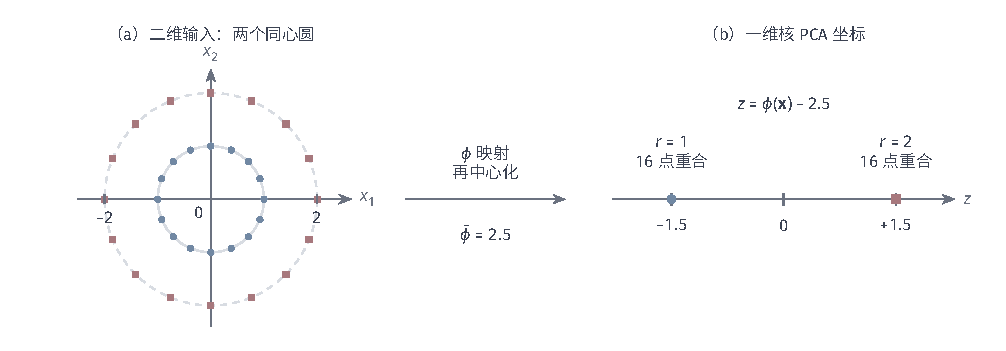
\includegraphics[width=169.000mm]{figures/03-models/01-classic-models/tikz/dim-kernel-radial/figure.pdf}
  \caption{由核选择保留量的构造例子。左图在半径为$1,2$的圆上各取16个等角度样本，圆点与方点区分两圈。所示特制核对应标量特征$\phi(\bm{x})=\lVert\bm{x}\rVert_2^2$，中心化核矩阵秩为1；选择图示主轴方向，核PCA坐标为$\pm1.5$。右侧每个标记表示16点重合，坐标无量纲。此结果依赖所选核，不能推广为任意高斯核或多项式核的输出。}
  \label{fig:dim-kernel-radial}
\end{figure*}

新样本必须沿用训练特征均值，才能与训练表示处于同一坐标系。令$\bm{k}(\bm{x})_i=K(\bm{x}_i,\bm{x})$，中心化及投影为
\begin{equation}
  \label{eq:dim-kpca-extension}
  \begin{aligned}
    \bm{k}_{\mathrm{c}}(\bm{x})
      ={}&\bm{k}(\bm{x})-\frac1n\bm{K}\bm{1}\\
         &-\frac1n\bm{1}\bm{1}^{\top}\bm{k}(\bm{x})
          +\frac1{n^2}\bm{1}\bm{1}^{\top}\bm{K}\bm{1},\\
    z_\ell(\bm{x})
      ={}&\bm{\alpha}_\ell^{\top}\bm{k}_{\mathrm{c}}(\bm{x}).
  \end{aligned}
\end{equation}
两个减项分别扣除与训练均值的内积，末项补回均值自内积。只减新核向量自身均值会漏掉这些量；加入新点重算均值，则是在改变原先的映射。

常用核的全矩阵构造约需$O(n^2d)$，存储为$O(n^2)$，稠密谱分解为$O(n^3)$。Nystr\"om近似使用代表列减少矩阵计算，随机Fourier特征则对合适的平移不变核构造有限特征后再做线性PCA。近似误差需要单独评价，适用核也各有条件。

高斯核带宽过大时，各核值接近，中心化信号变弱；带宽过小时，核矩阵接近单位阵，主方向难以辨认。距离中位数可作初始尺度，再用任务验证选择。监督任务中的中心化和主方向均应在训练折拟合。

\subsubsection{理论分析}
\label{sec:dim-kpca-theory}

\paragraph{表达能力}
核PCA在核特征空间中选择线性主方向，相对于原输入的非线性由特征映射提供。核、训练中心与保留维数共同限定表示；其高方差方向对下游任务是否有用，需要相应评价。

\paragraph{收敛性}

固定正定核后，经验方差目标可由谱分解全局求解，核矩阵近似及求谱精度决定数值误差。相同谱计算还连接点间距离：第\ref{sec:dim-mds}节定义经典MDS后，定理\ref{thm:dim-kpca-mds}将证明核诱导距离与中心化核PCA给出相同训练坐标。该联系针对特征距离，局部重构和图平滑则使用不同目标。

\paragraph{泛化性}

固定有界核、可分特征空间并独立同分布采样时，经验协方差算子随样本量增加逼近总体对象。目标谱与其余谱之间有正间隔，主子空间也可稳定逼近\scite{blanchard2007kpca}数据自适应核或趋零谱隙会改变分析所需条件。

样本外公式定义了新点的编码，并未评价分布外的质量；新点与训练点核值几乎相同时，表示可能缺少区分。若要重构原输入，还需另求截断特征的原像，有些特征甚至没有对应输入。

\subsubsection{小结}

核PCA先用核规定特征几何，再保留主要变化方向。谱求解与样本外公式使表示可复用，所得结果则依赖核合法性、训练中心化、带宽和谱隙。原空间几何的恢复还需要额外条件。

\subsection{模型对比与总结}
\label{sec:dim-linear-comparison}

矩阵形式相似的方法，保留的信息和编码成本可以不同。表\ref{tab:dim-linear-comparison}同时列出训练目标与新样本机制，分别回答怎样选表示、怎样复用表示。方形ICA保持维数，过完备稀疏编码甚至增加坐标数；它们在此共同使用线性投影或线性组合，但压缩方式各异。

\begin{table*}[htbp]
  \centering
  \small
  \begin{tabularx}{\linewidth}{@{}l>{\RaggedRight\arraybackslash}X>{\RaggedRight\arraybackslash}X>{\RaggedRight\arraybackslash}X@{}}
    \toprule
    方法 & 主要目标与约束 & 新样本的表示 & 典型边界\\
    \midrule
    PCA & 正交投影下保留方差 & 中心化后矩阵乘法 & 对尺度、异常值敏感\\
    CCA & 配对视图的相关性最大 & 两侧分别线性投影 & 需配对观测，易过拟合相关性\\
    ICA & 独立源的线性解混 & 白化及解混乘法 & 独立性、非高斯性与可识别性\\
    NMF & 非负基与非负系数重构 & 非负约束推断 & 非凸、通常不唯一\\
    稀疏编码 & 少量原子重构观测 & 稀疏优化 & 可为高维编码，需控制推断成本\\
    随机投影 & 随机矩阵近似保距 & 固定矩阵乘法 & 维数、误差与失败概率的权衡\\
    核PCA & 特征空间方差 & 训练中心化核投影 & 核几何、样本展开与原空间重构\\
    \bottomrule
  \end{tabularx}
  \caption{线性投影与线性组合方法的比较。目标成立均依赖各小节的具体条件；“新样本可编码”不等于编码具有统计泛化保证。}
  \label{tab:dim-linear-comparison}
\end{table*}

求解方式进一步决定预算：PCA与CCA作谱分解，ICA优化非高斯对比量，NMF与字典学习交替更新，随机投影生成固定矩阵。迭代方法还需计入稀疏结构、停止精度与总轮数。基可以追溯原始特征，是否对应可解释概念仍要由数据和任务验证。

响应或类别已知时，可以直接寻找与预测有关的方向。第\ref{sec:regression-regularization}节的PCR按输入方差选成分，PLS让响应参与构造；第\ref{sec:classification-lda-reduction}节的线性判别分析比较类间和类内散度。切片逆回归利用$\mathbb{E}[\bm{x}\mid y]$的变化，在相应线性及非退化条件下恢复有效方向，对条件均值无法显示的对称响应则可能遗漏\scite{li1991sir}这些目标把任务信息加入方向选择，改变了单纯保留输入方差的准则。

监督降维组合特征形成新方向，特征选择保留原坐标子集，两者可以共同使用。比较预测收益时，应将响应参与的方向学习、特征选择和预测器都放在训练折内，以相同下游风险比较无监督表示、监督表示和不降维基线。

选择线性组合时，需要先确定保留的是方差、视图相关、独立源、非负成分、稀疏支持还是点对距离。第\ref{sec:dim-probabilistic}节的因子分析会加入特征特异噪声；下一节MDS则从距离恢复坐标，并在欧氏输入下联系PCA。弯曲结构若无法由原空间线性基充分描述，还需要不同的特征或非线性关系。

\section{基于距离的降维}
\label{sec:dim-distance}

对象之间的差异有时比原始坐标更容易取得，例如相似性评分或编辑距离。此时需要根据差异安排位置，而非直接投影特征。多维缩放提供了这种坐标恢复；下一节还会把差异限制到局部邻域，用来研究弯曲几何。

\subsection{多维缩放（MDS）}
\label{sec:dim-mds}

感知评分给出对象间差异，却没有给出对象坐标。\term{多维缩放}（multidimensional scaling, MDS）寻找低维位置，使坐标关系尽量符合这些差异。Young与Householder于1938年研究距离对坐标的代数约束，为坐标恢复建立了几何依据\scite{dimYoung1938}

Torgerson在1952年系统提出经典MDS时，还要处理心理距离怎样测量。刺激比较的差异可能缺少确定零点，因此原工作先估计比较距离中的未知加性常数，再分析维数和刺激坐标\scite{dimTorgerson1952}差异输入本身也有测量假设，这里的加性常数与下面的坐标、核矩阵中心化承担不同作用。

\subsubsection{模型结构}

将对象差异记为对称矩阵$\bm{D}\in\mathbb{R}^{n\times n}$，要求$\bm{D}_{i,j}\geq0$、$\bm{D}_{i,i}=0$。它可以来自欧氏、编辑、图距离或人工评分；这些关系未必能在指定维数中由欧氏距离实现。MDS的拟合准则决定采用哪一种近似。

要恢复欧氏几何，可以先从距离平方求中心化内积。\term{经典MDS}（classical MDS）采用这一转换，令$\bm{1}\in\mathbb{R}^n$为全一向量、$\bm{I}_n$为单位矩阵：
\begin{equation}
  \label{eq:dim-mds-centering}
  \begin{aligned}
    \bm{H}&=\bm{I}_n-\frac{1}{n}\bm{1}\bm{1}^{\top},\\
    \bm{D}^{\circ2}_{i,j}&=(\bm{D}_{i,j})^2,\\
    \bm{B}&=-\frac12\bm{H}\bm{D}^{\circ2}\bm{H}.
  \end{aligned}
\end{equation}
$\circ2$是逐元素平方。左右乘$\bm{H}$分别扣去列、行均值，即双中心化；欧氏输入得到的$\bm{B}$是中心化坐标的Gram矩阵，记录两两内积且为半正定。

从$\bm{B}$的正谱取得实数坐标。记$\lambda_1\geq\cdots\geq\lambda_r>0$，相应欧氏单位特征向量为$\bm{u}_1,\ldots,\bm{u}_r$；选择$k\leq r$后，坐标为
\begin{equation}
  \label{eq:dim-mds-coordinates}
  \bm{Z}=\bm{U}_k\bm{\Lambda}_k^{1/2},
  \qquad
  \bm{Z}_{i,\ell}=\sqrt{\lambda_\ell}\,(\bm{u}_\ell)_i.
\end{equation}
$\bm{U}_k$收集所选特征向量，$\bm{\Lambda}_k$收集相应特征值。其平方根缩放使坐标内积逼近$\bm{B}$，最小化的内积残差称为strain：
\begin{equation}
  \label{eq:dim-mds-strain}
  \min_{\substack{\bm{Z}\in\mathbb{R}^{n\times k}\\
                  \bm{Z}^{\top}\bm{1}=\bm{0}}}
  \left\lVert\bm{B}-\bm{Z}\bm{Z}^{\top}\right\rVert_{\mathrm{F}}^2.
\end{equation}
非欧氏差异可能使$\bm{B}$含负特征值。半正定秩约束近似舍弃负谱，保留最大的至多$k$个正特征值；这种内积近似通常也会改变输入距离。

任务若直接比较距离数值，可以让\term{度量MDS}（metric MDS）最小化距离残差。给定对称非负权重$w_{i,j}$，记$\delta_{i,j}(\bm{Z})=\lVert\bm{z}_i-\bm{z}_j\rVert_2$，常用应力（stress）目标为
\begin{equation}
  \label{eq:dim-mds-stress}
  S(\bm{Z})
  =\sum_{i<j}w_{i,j}
    \bigl(\delta_{i,j}(\bm{Z})-\bm{D}_{i,j}\bigr)^2.
\end{equation}
strain比较内积，stress比较距离。虽然距离与中心化内积可互相转换，两种残差平方和仍有不同的最优近似。有些文献也将经典MDS称为metric scaling，本章按实际目标区分。

当差异顺序比数值更可信时，\term{非度量MDS}（nonmetric MDS）用非递减函数$g(\bm{D}_{i,j})$作为式\eqref{eq:dim-mds-stress}中的目标距离，同时估计$g$和$\bm{Z}$。尺度约束排除共同缩到零的退化，保序要求作用于拟合差异；有限维坐标仍可能无法满足所有严格次序。Kruskal于1964年将顺序信息与应力准则结合\scite{dimKruskal1964}

\subsubsection{参数学习}

经典MDS的平方Frobenius目标可以沿正交特征方向分解。半正定约束排除负谱，秩约束保留较大的正谱，因此双中心化和谱截断给出全局最优表达；特征向量仍需数值求解。

距离残差通常采用迭代拟合，也可以按距离选择权重。例如所有非对角距离$\bm{D}_{i,j}>0$时，\term{Sammon映射}使用
\begin{equation}
  \label{eq:dim-sammon}
  S_{\mathrm{Sammon}}(\bm{Z})
  =\frac{1}{\sum_{i<j}\bm{D}_{i,j}}
    \sum_{i<j}
    \frac{\bigl(\delta_{i,j}(\bm{Z})-\bm{D}_{i,j}\bigr)^2}
         {\bm{D}_{i,j}}.
\end{equation}
小距离的相同绝对误差在此受到更大惩罚，使局部距离更受重视。它仍是近似目标，零差异需要合并对象或另定权重\scite{dimSammon1969}

应力型MDS可用梯度法、拟牛顿法，或\term{SMACOF}（scaling by majorizing a complicated function）。SMACOF在当前坐标构造与目标相切的二次上界，再最小化该上界；记上界为$Q$，下降关系为
\[
  S(\bm{Z}^{(s+1)})
  \leq Q(\bm{Z}^{(s+1)}\mid\bm{Z}^{(s)})
  \leq Q(\bm{Z}^{(s)}\mid\bm{Z}^{(s)})
  =S(\bm{Z}^{(s)}).
\]
非度量MDS可以交替求保序回归和坐标更新。目标非负且不增加时，目标值收敛；迭代点是否到达驻点、极小或全局最优仍要另查。实践中可以用经典MDS初始化并比较多次运行，SMACOF的构造与实现见de Leeuw和Mair的系统介绍\scite{dimDeLeeuw2009}

完整稠密经典MDS需要$O(n^2)$存储，谱分解通常为$O(n^3)$。部分谱或Nystr\"om近似可以减少计算；标志点MDS先嵌入代表点，再按到代表点的距离扩展，近似质量依赖代表点的覆盖。

\subsubsection{理论分析}
\label{sec:dim-mds-theory}

\paragraph{表达能力}
MDS以低维点间几何拟合距离或相异度。指定维数中的欧氏关系有结构限制，任意相异度未必满足，因此谱截断和应力拟合都可能留下无法消除的失真。

\paragraph{收敛性}

经典MDS的全局最优针对内积目标；应力型MDS的迭代通常在适当条件下保证下降。要进一步联系PCA，需要让两者处理同一批欧氏观测，并比较同一中心化坐标的谱截断。

设$\bm{D}$来自坐标矩阵$\bm{X}$各行的欧氏距离，中心化坐标为$\bm{X}_{\mathrm{c}}=\bm{H}\bm{X}$。平移不改变这些距离，双中心化得到
\[
  \bm{B}=\bm{H}\bm{X}\bm{X}^{\top}\bm{H}
  =\bm{X}_{\mathrm{c}}\bm{X}_{\mathrm{c}}^{\top}.
\]
该Gram矩阵来自中心化后的$\bm{X}_{\mathrm{c}}$。选择相同维数和相应奇异方向时，PCA与经典MDS共享谱截断；证明的关键是展开距离平方，说明双中心化怎样消去平移项并恢复该Gram矩阵。

\begin{theorem}[欧氏距离下经典MDS与PCA的关系]
  \label{thm:dim-mds-pca}
  设$\bm{X}^{\top}\bm{1}=\bm{0}$，$\bm{D}_{i,j}=\lVert\bm{x}_i-\bm{x}_j\rVert_2$，且$1\leq k\leq\operatorname{rank}(\bm{X})$。若PCA与经典MDS选取相互对应的前$k$个奇异方向，则两者的坐标都可取为$\bm{U}_k\bm{\Sigma}_k$，从而得到相同的坐标Gram矩阵$\bm{U}_k\bm{\Sigma}_k^2\bm{U}_k^{\top}$。同一所选子空间内的坐标可相差右侧正交变换，而Gram矩阵保持不变。
\end{theorem}
\begin{proof}
  令$\bm{a}\in\mathbb{R}^n$满足$a_i=\lVert\bm{x}_i\rVert_2^2$。展开距离平方并双中心化，得到
  \[
    \begin{aligned}
      \bm{D}^{\circ2}
        &=\bm{a}\bm{1}^{\top}+\bm{1}\bm{a}^{\top}
          -2\bm{X}\bm{X}^{\top},\\
      \bm{B}
        &=\bm{H}\bm{X}\bm{X}^{\top}\bm{H}
         =\bm{X}\bm{X}^{\top}.
    \end{aligned}
  \]
  第一、第二项消失，是因为$\bm{H}\bm{1}=\bm{0}$；末步使用样本已经中心化。对薄奇异值分解$\bm{X}=\bm{U}\bm{\Sigma}\bm{V}^{\top}$，有$\bm{B}=\bm{U}\bm{\Sigma}^2\bm{U}^{\top}$。MDS坐标与PCA得分因而分别为
  \[
    \bm{Z}_{\mathrm{MDS}}=\bm{U}_k\bm{\Sigma}_k,
    \qquad
    \bm{X}\bm{V}_k=\bm{U}_k\bm{\Sigma}_k.
  \]
  在同一所选子空间内旋转坐标轴不改变Gram矩阵。
\end{proof}

等价对象是同一保留维数$k$下的中心化坐标Gram矩阵及其诱导距离，原特征轴并未恢复。只有$k=\operatorname{rank}(\bm{X}_{\mathrm{c}})$、保留全部正特征值时，坐标才保留全部输入欧氏距离；$k<\operatorname{rank}(\bm{X}_{\mathrm{c}})$时，两者共享一个改变原距离的谱截断。

截断若满足$\lambda_k=\lambda_{k+1}$，可以选择不同的最优部分子空间，结果未必只差一个$k$维旋转。小谱隙也使方向对距离扰动敏感；评价稳定性时可比较对齐坐标、子空间或重构距离。

核特征距离也具有同一内积展开，因而第\ref{sec:dim-kpca}节预告的联系可以按相同方式证明。

\begin{theorem}[核诱导距离下的等价关系]
  \label{thm:dim-kpca-mds}
  设$K$为正定核，记$\bm{K}_{i,j}=K(\bm{x}_i,\bm{x}_j)$。训练点间的特征距离为
  \[
    \bm{D}_{i,j}^2
    =\bm{K}_{i,i}+\bm{K}_{j,j}-2\bm{K}_{i,j}.
  \]
  对此距离进行经典MDS，与对$\bm{K}$进行中心化核PCA，在选择相同正特征子空间和归一化后给出相同训练坐标。重特征值和截断处的非唯一性与定理\ref{thm:dim-mds-pca}相同。
\end{theorem}
\begin{proof}
  令向量$\bm{a}$的元素$a_i=\bm{K}_{i,i}$，距离平方矩阵为$\bm{a}\bm{1}^{\top}+\bm{1}\bm{a}^{\top}-2\bm{K}$。双中心化消去前两项，得到$\bm{B}=\bm{H}\bm{K}\bm{H}=\bm{K}_{\mathrm{c}}$。式\eqref{eq:dim-mds-coordinates}与式\eqref{eq:dim-kpca-training}因而输出相同的$\bm{U}_k\bm{\Lambda}_k^{1/2}$。
\end{proof}

\paragraph{泛化性}

新样本上的使用需要分开看统计估计和坐标扩展。距离来自独立同分布欧氏观测时，MDS与PCA的等价关系可以接入协方差估计分析；任意差异矩阵则要另给差异的生成机制和估计误差。

新对象到训练对象的距离已知时，可以固定原坐标作经典MDS扩展。记这些距离平方为$s_i$，$\bar s=n^{-1}\sum_i s_i$；训练距离的行均值为$r_i=n^{-1}\sum_j\bm{D}_{i,j}^2$，总均值为$\bar r=n^{-1}\sum_i r_i$。相对训练中心的内积与坐标为
\begin{equation}
  \label{eq:dim-mds-extension}
  \begin{aligned}
    b_i&=-\frac12(s_i-\bar s-r_i+\bar r),\\
    \bm{z}(\bm{x})
      &=\bm{\Lambda}_k^{-1/2}\bm{U}_k^{\top}\bm{b}.
  \end{aligned}
\end{equation}
第一行沿用训练中心计算内积，第二行用最小二乘取得相应坐标。训练点保持固定，与加入新点重做MDS的结果不同；非欧氏差异下，该扩展是相对已有表示的近似投影\scite{dimBengio2003}

\subsubsection{小结}

MDS根据差异安排坐标，经典、度量与非度量形式分别拟合内积、距离与顺序。相同欧氏观测和相同保留维数下，经典MDS与中心化PCA共享谱截断；降到数据秩以下，两者都会改变原距离。距离的可嵌入性、截断维数与矩阵规模共同限定结果。

\subsection{模型对比与总结}

已有特征且关心方差，可以直接用PCA学习投影；只有对象差异时，可以用MDS安排位置。选择MDS的形式，要确认输入表达的是内积几何、距离数值还是可信顺序，再用相应目标和样本外机制评价。不同目标的数值没有直接可比性。

\section{基于邻域的降维}
\label{sec:dim-neighbors}
\label{sec:dim-manifold}

如果原空间距离主要在小范围内可信，可以先建立邻域，再组织全局坐标。第\ref{sec:classic-overview-neighborhood}节给出了邻域与图的共同机制；这里按要保留的关系展开：图路径描述长度，局部组合描述重构，图上平滑和随机游走描述连通性，邻居概率或边权则用于安排可观察的布局。

几何方法中的部分模型假设数据接近\term{流形}（manifold），即局部可以用少量连续坐标描述的空间。弯曲结构的方向随位置改变，直接投影可能混合沿曲面相距较远的点；局部自由度少，整体却仍可能无法在同维数中无失真展开。各方法需要的采样和几何条件将在具体构造中给出。

以下继续使用$n,d,k,m,q$与$\bm{X},\bm{Z}$。布局的输入距离记为$\delta_{i,j}=\lVert\bm{x}_i-\bm{x}_j\rVert_2$，低维距离记为$r_{i,j}=\lVert\bm{z}_i-\bm{z}_j\rVert_2$。训练坐标是这些方法直接求得的对象，接收新样本还需规定相应映射或扩展。

\subsection{等距映射（Isomap）}
\label{sec:dim-isomap}

弯曲流形上，穿过观测空间的直线距离与沿流形的最短长度可以相差很大。后者为\term{测地距离}（geodesic distance），记为$d_{\mathcal{M}}$。\term{等距映射}（isometric mapping, Isomap）用邻域图最短路径估计它，再由经典MDS恢复坐标。Tenenbaum、de Silva与Langford于2000年提出该方法；同年的LLE则选择局部重构关系作为保留对象\scite{dimTenenbaum2000}

\subsubsection{模型结构}

将样本作为顶点建立无向图$\mathcal{G}=(V,E)$，连接距离不超过$\varepsilon$的点，或对称化$q$近邻。近邻并集与互近邻给出的边不同，需要明确采用哪一种。每条边的长度为$\ell_{i,j}=\lVert\bm{x}_i-\bm{x}_j\rVert_2$，是路径成本；长度越小越近，与后文连接越强数值越大的相似度权重不同。

路径只能沿图中边行走。将一条路径的边长相加，再在全部可行路径中选择最短者：
\begin{equation}
  \label{eq:dim-isomap-distance}
  d_{\mathcal{G}}(i,j)
  =\min_{\substack{i=i_0,\ldots,i_s=j\\(i_{a-1},i_a)\in E}}
    \sum_{a=1}^{s}\ell_{i_{a-1},i_a}.
\end{equation}
由全部图距离组成$\bm{D}_{\mathcal{G}}$，计算$\bm{B}_{\mathcal{G}}=-\tfrac12\bm{H}\bm{D}_{\mathcal{G}}^{\circ2}\bm{H}$，再按式\eqref{eq:dim-mds-coordinates}取坐标。局部连接、全局路径和欧氏表示依次承担三项工作；路径近似与MDS拟合也分别引入误差。

邻域决定路径能否合理近似曲面长度。图\ref{fig:dim-geodesic}中的两段曲线在观测空间接近，沿曲线却相距很远；跨过弯曲部分的一条错误边，可能缩短许多点对的图距离。
\begin{figure}[htbp]
  \centering
  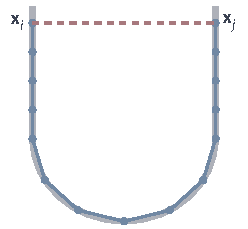
\includegraphics[width=42.012mm]{figures/03-models/01-classic-models/tikz/dim-geodesic/figure.pdf}
  \caption{一维弯曲曲线上的距离示意。曲线表示嵌入观测空间的一维流形，曲线上的点表示离散样本；沿相邻样本连接的折线表示邻域图路径，其各段长度之和用于近似沿曲线的测地距离。顶部红色虚线是两点间的欧氏直线；若邻域取值过大而把它误纳入图中，就会形成穿过流形外部、低估测地距离的短路。图为几何示意，不是算法输出或实验结果，未给出数值误差。}
  \label{fig:dim-geodesic}
\end{figure}

\subsubsection{参数学习}

暴力建邻域约需$O(n^2d)$时间，空间索引的收益依赖维数与分布。非负边长下，从每点运行二叉堆Dijkstra的成本为$O(n(|E|+n)\log n)$，Floyd--Warshall为$O(n^3)$。后续稠密MDS仍需$O(n^2)$存储、通常$O(n^3)$的完整谱分解；稀疏邻域并未使全体点对距离也稀疏。

输入度量、预处理、$q$或$\varepsilon$以及$k$共同决定结果。小邻域可能断连，大邻域可能跨过卷层，噪声和非均匀采样也会改变可用尺度。可检查连通分量、边长分布及随邻域变化的稳定性。距离相关残差$1-R^2$提供辅助诊断，但对统一缩放不敏感，仍需直接检查失真与测地近似。

标志点Isomap（Landmark Isomap）选$s\ll n$个代表点，从这些点出发求最短路径，保留$s\times n$距离表，再用标志点MDS和距离扩展安排其余点。de Silva与Tenenbaum的原文还讨论共形变换下的距离修正\scite{dimDeSilva2002}标志点减少计算规模，共形修正改变几何假设，是两项不同的选择。

\subsubsection{理论分析}
\label{sec:dim-isomap-theory}

\paragraph{表达能力}
Isomap的表示由两层近似组成：邻域最短路径拟合测地距离，低维欧氏坐标拟合图距离。错误捷径或无法等距展开的流形，会使同时保留全部距离的目标难以实现。

\paragraph{收敛性}
固定图后，最短路径算法求出图距离，经典MDS求相应的谱近似。数值精度可以通过路径与谱求解检查，邻域是否近似真实几何则属于建模条件；计算完成并未消除两层近似的误差。

\paragraph{泛化性}
样本增加时，希望图距离也越来越接近测地距离。覆盖不足会漏掉必要连接，边长失真过大又会形成捷径，下面的确定性界分别控制这两种问题。

覆盖空隙$h$衡量流形上各位置到最近样本的最大测地距离，单边失真$\eta$衡量弦长比测地距离短多少。证明沿最短测地线放置分割点，再用附近样本替代它们，构造图路径以控制误差；这里尚未要求该距离能嵌入指定$k$维。

\begin{theorem}[覆盖条件下的图距离界]
  \label{thm:dim-isomap-bound}
  设$\mathcal{M}\subset\mathbb{R}^d$连通，任意两点间存在最短测地线。样本的测地填充距离为
  \[
    h=\sup_{\bm{x}\in\mathcal{M}}\min_i
      d_{\mathcal{M}}(\bm{x},\bm{x}_i).
  \]
  图连接全部欧氏距离不超过$\varepsilon$的样本对，并以欧氏弦长为边长。假设$h<\varepsilon/2$，且存在$0\leq\eta<1$，使每条边都满足
  \[
    \lVert\bm{x}_i-\bm{x}_j\rVert_2
    \geq(1-\eta)d_{\mathcal{M}}(\bm{x}_i,\bm{x}_j).
  \]
  则对所有样本对，图距离有限，且
  \begin{equation}
    \label{eq:dim-isomap-bound}
    \begin{aligned}
      d_{\mathcal{G}}(i,j)
        &\geq(1-\eta)d_{\mathcal{M}}(\bm{x}_i,\bm{x}_j),\\
      d_{\mathcal{G}}(i,j)
        &\leq\left(1+\frac{2h}{\varepsilon-2h}\right)
          d_{\mathcal{M}}(\bm{x}_i,\bm{x}_j).
    \end{aligned}
  \end{equation}
\end{theorem}
\begin{proof}
  对任意图路径，各边弦长至少是对应测地距离的$1-\eta$倍。将其相加，再用测地距离的三角不等式，就得到下界。

  为证明上界，记两端点的测地距离为$L$，取连接它们的一条最短测地线，令$a=\varepsilon-2h>0$。若$L=0$，结论成立；否则沿测地线每隔$a$放一个分割点，末段不足$a$，总段数为$s=\lceil L/a\rceil$。保留原来的两个样本端点，把每个内部分割点替换成测地距离不超过$h$的样本。相邻替代样本的测地距离至多$a+2h=\varepsilon$，欧氏距离不更大，因此构成图中的边；重复样本可略去。

  每个内部分割点的替代误差至多在两条相邻边中各计一次，而两端点无需替代，故所构造路径的长度至多
  \[
    L+2h(s-1)
    \leq L+\frac{2hL}{\varepsilon-2h}.
  \]
  图最短路径不长于这条路径，得到上界，同时证明图中这些端点相连。
\end{proof}

对一列样本与邻域，若$h/\varepsilon\to0$且$\eta\to0$，两侧界给出样本点对上的统一相对距离一致性。曲率有界仍需配合足够小的邻域尺度，才能排除卷层间连接。若采样独立且密度有正下界，可以研究覆盖空隙$h$的概率界，条件还需包括体积、内在维数、覆盖数和密度。

图距离准确之后，还要判断是否存在欧氏坐标保留它。单位球面赤道上四个等间隔点，相邻测地距离为$\pi/2$，两组对点为$\pi$。若都能成为欧氏距离，三角不等式取等号迫使另外两点成为同一对点的中点；它们却应相距$\pi$，产生矛盾。这说明真实测地距离本身也可能无法同时欧氏实现。

当流形与$\mathbb{R}^m$中凸区域在长度意义下等距时，区域内测地长度就是直线距离，这是恢复平直坐标的一类充分情形。带孔非凸区域即使局部平直，绕孔长度仍可能不同。后续MDS还需控制距离误差对内积和谱子空间的影响。新点可通过到邻居的边长加训练图距离，再用式\eqref{eq:dim-mds-extension}定位；原图固定，不等于加入点后重新计算全体最短路径。

\subsubsection{小结}

Isomap将局部边长汇总成全局长度，适合考察可展开的几何结构。覆盖、无短路邻域与目标欧氏维数共同决定可靠性。断连分量之间没有有限路径，需分别处理或依据额外信息连接；随意填入大数会引入新的距离假设。

\subsection{局部线性嵌入（LLE）}
\label{sec:dim-lle}

局部邻域还能提供另一种约束：一个点由哪些邻居、按什么权重重构。\term{局部线性嵌入}（locally linear embedding, LLE）将样本写成邻居的仿射组合，再要求低维坐标保持这些组合关系。它用距离选邻居、用局部内积求权重，但不计算全体点对的路径距离。

LLE与Isomap在2000年同一期《Science》上相邻发表，都利用局部信息建立全局坐标。LLE原文致谢中记载了作者与Tenenbaum的讨论，以及对方提供Isomap代码的帮助\scite{dimRoweis2000}两项工作有实际交流，采用的约束却不同：Isomap拟合路径长度，LLE拟合局部重构关系。

\subsubsection{模型结构}

令$\mathcal{N}_i$包含样本$i$的$q$个邻居。重构矩阵$\bm{W}\in\mathbb{R}^{n\times n}$只在邻居位置取非零权重，且每行权重和为一。通过最小化原空间的重构残差求这些权重：
\begin{equation}
  \label{eq:dim-lle-weights}
  \begin{aligned}
    \min_{\bm{W}}\quad&
      \sum_i\left\lVert\bm{x}_i-\sum_j\bm{W}_{i,j}\bm{x}_j
      \right\rVert_2^2,\\
    \text{满足}\quad&
      \bm{W}\bm{1}=\bm{1},\qquad
      \bm{W}_{i,j}=0\quad(j\notin\mathcal{N}_i).
  \end{aligned}
\end{equation}
行和为一使重构关系对整体平移不变：所有点加上同一个向量，中心点及其重构点同步移动。权重可以为负，因此组合是仿射的，未必是凸的。$\bm{W}$通常不对称，其元素也不能解释为随机游走概率。

固定$\bm{W}$后，在低维空间最小化同一组权重对应的残差。记$\bm{M}=(\bm{I}_n-\bm{W})^{\top}(\bm{I}_n-\bm{W})$，目标为
\begin{equation}
  \label{eq:dim-lle-embedding}
  \begin{aligned}
    \min_{\bm{Z}}\quad&
      \lVert(\bm{I}_n-\bm{W})\bm{Z}\rVert_{\mathrm{F}}^2
      =\operatorname{tr}(\bm{Z}^{\top}\bm{M}\bm{Z}),\\
    \text{满足}\quad&
      \bm{Z}^{\top}\bm{1}=\bm{0},\qquad
      \bm{Z}^{\top}\bm{Z}=n\bm{I}_k.
  \end{aligned}
\end{equation}
样本按行排列，因而残差写作$(\bm{I}_n-\bm{W})\bm{Z}$。中心化约束去掉整体平移，列正交与定范数约束防止坐标全部塌缩。这里选定的是代数尺度，未要求坐标距离等于原始距离。

图\ref{fig:dim-lle-weights}用权重$0.3,0.3,0.4$重构中心点。邻居移动后，以同一权重安排中心仍可得到零残差，三角形边长却已改变。完整LLE还需协调其他点的邻域并满足全局约束，图中只展示一项局部关系。

\begin{figure*}[htbp]
  \centering
  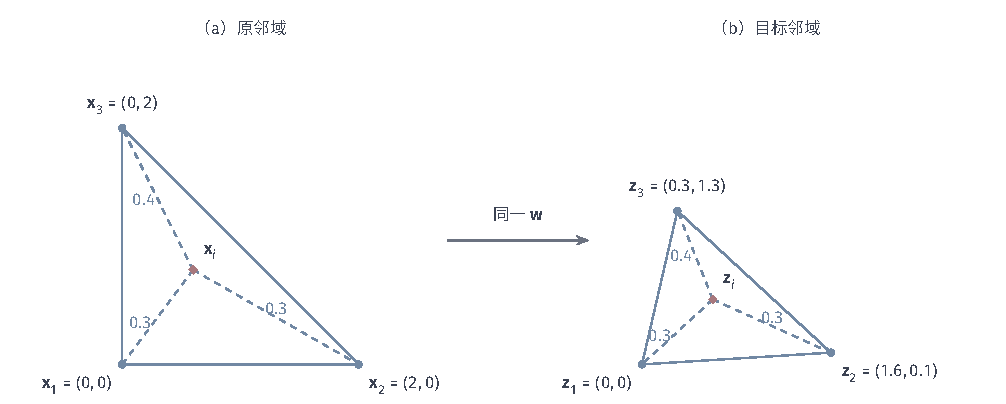
\includegraphics[width=169.000mm]{figures/03-models/01-classic-models/tikz/dim-lle-weights/figure.pdf}
  \caption{LLE局部权重保持的示意。左图用二维局部坐标绘出三个邻居和菱形中心点；虚线旁为重构权重，其和为1。右图将邻居移至所标位置，同样的权重给出中心$(0.60,0.55)^\top$。两图使用相同的无量纲尺度，实线三角形的形状与边长可以改变。两个画面用于对照高维局部几何与目标邻域，不是完整LLE输出，也不表示一次二维到二维的降维。}
  \label{fig:dim-lle-weights}
\end{figure*}

\subsubsection{参数学习}

按固定顺序排列第$i$个邻域，令$\bm{A}_i\in\mathbb{R}^{q\times d}$的每行为$(\bm{x}_j-\bm{x}_i)^{\top}$，并记$\bm{C}_i=\bm{A}_i\bm{A}_i^{\top}$。该邻域的权重$\bm{w}_i\in\mathbb{R}^q$满足
\[
  \min_{\bm{1}^{\top}\bm{w}_i=1}
    \bm{w}_i^{\top}\bm{C}_i\bm{w}_i.
\]
当$\bm{C}_i$正定时，驻点条件为$\bm{C}_i\bm{w}_i=c\bm{1}$。用权重和为一确定$c$，得到
\begin{equation}
  \label{eq:dim-lle-local}
  \bm{w}_i
  =\frac{\bm{C}_i^{-1}\bm{1}}
         {\bm{1}^{\top}\bm{C}_i^{-1}\bm{1}}.
\end{equation}
求权重时直接解线性方程即可。$q>d$使$\bm{C}_i$必然奇异；即使$q\leq d$，局部样本接近低维切空间也可能造成秩亏或病态。可用$\bm{C}_i+\rho_i\bm{I}_q$改善条件数，例如令$\rho_i$与迹成比例。邻居全部重合时迹为零，需另设正的尺度下限或单独处理。加入正则项也改变了原重构目标。

行和约束给出$\bm{M}\bm{1}=\bm{0}$。在常数方向的正交补中，取最小的$k$个特征方向组成单位列矩阵$\bm{U}_k$，则$\bm{Z}=\sqrt n\,\bm{U}_k$解式\eqref{eq:dim-lle-embedding}。零空间只有常数方向时，才能取最小$k+1$个特征向量后丢掉一个。断连分量的指示向量也属于零空间；对于带符号权重，连通本身仍不足以保证零空间只有一维。

额外零模态会使部分坐标只给各分量分配常数，未表达分量内部的形状。分别嵌入各分量也无法由局部关系确定它们的相对位置、方向和尺度，断连问题仍需额外处理。

局部矩阵构造及求解约需$O(nq^2d+nq^3)$。全局阶段可依次乘$\bm{I}_n-\bm{W}$及其转置，无需显式形成$\bm{M}$；一次矩阵向量乘约为$O(nq)$。部分谱求解还受谱隙、迭代次数和重正交成本影响。邻居数$q$、输出维数$k$与正则尺度都需要选择。

局部重构关系为何可能在降维后保留，可以用坐标函数的Taylor展开解释。令邻居的局部位移为$\bm{\xi}_j$，对光滑函数$f$有
\[
  \begin{aligned}
    f(\bm{x}_i)-\sum_j\bm{W}_{i,j}f(\bm{x}_j)
    ={}&-\nabla f^{\top}\sum_j\bm{W}_{i,j}\bm{\xi}_j\\
       &+O\left(\sum_j|\bm{W}_{i,j}|
                  \lVert\bm{\xi}_j\rVert_2^2\right).
  \end{aligned}
\]
权重和为一消去常数项，加权位移接近零又使一阶项较小，剩余误差主要来自二阶变化。余项中出现权重绝对值，所以大幅正负抵消可能放大误差。噪声还会改变邻域和局部矩阵，局部近似是否可靠需要另行检查。

对新点先求局部重构权重，再以$\bm{z}(\bm{x})=\sum_{j\in\mathcal{N}(\bm{x})}w_j(\bm{x})\bm{z}_j$插值。训练坐标固定，这一步未重新求全局谱。邻域不稳定或新点远离训练支持时，插值可能失真。

\subsubsection{小结}

LLE以局部仿射关系连接各邻域，可靠性取决于邻域尺度、局部秩、权重稳定性和全局零空间。它省去全体点对最短路径，却未要求距离或角度精确保留。Hessian LLE增加局部二阶约束，局部切空间对齐（LTSA）估计并对齐切空间；本节比较将说明这些约束及其适用条件。

\subsection{拉普拉斯特征映射（Laplacian Eigenmaps）}
\label{sec:dim-le}

邻近点的坐标变化缓慢，也能成为降维约束。\term{拉普拉斯特征映射}（Laplacian Eigenmaps）将这种平滑性写成图上的二次能量，在防止塌缩的约束下求低能量坐标。Belkin与Niyogi在NIPS 2001介绍相关谱方法，2003年期刊论文展开其模型与几何联系\scite{dimBelkin2003}它与第\ref{sec:clustering-spectral}节的谱聚类共享建图、图拉普拉斯与低频特征方向；这里直接输出连续坐标，谱聚类再将谱表示转成簇分配。

\subsubsection{模型结构}

在对称邻域图上设非负权重$\bm{W}_{i,j}$。相邻点可取$\exp(-\lVert\bm{x}_i-\bm{x}_j\rVert_2^2/(4\tau))$或$1$，其他位置为零，$\tau>0$控制衰减尺度。令$b_i=\sum_j\bm{W}_{i,j}$、$\bm{D}_b=\operatorname{diag}(b_1,\ldots,b_n)$，图拉普拉斯为$\bm{L}=\bm{D}_b-\bm{W}$。对标量信号$\bm{f}\in\mathbb{R}^n$，由对称性有
\begin{equation}
  \label{eq:dim-le-energy}
  \bm{f}^{\top}\bm{L}\bm{f}
  =\frac12\sum_{i,j}\bm{W}_{i,j}(f_i-f_j)^2.
\end{equation}
能量非负，故$\bm{L}$半正定，常数信号的能量为零。将各坐标列的能量相加，得到
\begin{equation}
  \label{eq:dim-le-objective}
  \begin{aligned}
    \min_{\bm{Z}}\quad&
      \operatorname{tr}(\bm{Z}^{\top}\bm{L}\bm{Z}),\\
    \text{满足}\quad&
      \bm{Z}^{\top}\bm{D}_b\bm{Z}=\bm{I}_k,\qquad
      \bm{Z}^{\top}\bm{D}_b\bm{1}=\bm{0}.
  \end{aligned}
\end{equation}
度加权范数排除零解，加权中心化排除常数方向。缺少后一个约束，就可能将没有区分能力的常数列纳入嵌入。目标只惩罚邻近点的坐标差异，远点是否分开还由全局约束和所选模式决定。

\subsubsection{参数学习}

对坐标列求驻点，在常数的加权正交补中得到$\bm{L}\bm{v}=\lambda\bm{D}_b\bm{v}$。各点度为正时，令$\bm{u}=\bm{D}_b^{1/2}\bm{v}$，将它化成对称特征值问题：
\[
  \bm{L}_{\mathrm{sym}}\bm{u}=\lambda\bm{u},
  \qquad
  \bm{L}_{\mathrm{sym}}
  =\bm{I}_n-\bm{D}_b^{-1/2}\bm{W}\bm{D}_b^{-1/2}.
\]
求得单位向量后，要变回$\bm{v}=\bm{D}_b^{-1/2}\bm{u}$以满足模型的归一化。连通图的广义问题以常数为零特征向量，对称问题的零方向却与$\bm{D}_b^{1/2}\bm{1}$成比例。多个连通分量对应多个零模态，应一并识别；零度点也需单独处理，不能直接作逆度归一化。

若权重矩阵有$O(nq)$个非零元，一次矩阵向量乘为$O(nq)$。总求解成本还包括建图、$k$个方向的迭代及正交化。$q$控制哪些点连接，$\tau$控制连接强弱，$k$控制保留的模式数。过小带宽可能使部分度数接近零，过大带宽则削弱局部差异，可结合图诊断与任务表现选择。

\subsubsection{理论分析}
\label{sec:dim-le-theory}

\paragraph{表达能力}
表示由图上的低频模式组成，输出维数限定保留多少模式。它保留邻域平滑关系，但这些关系未必唯一确定全局几何；任务所需的快速变化也可能被截断。

\paragraph{收敛性}
固定非负邻域图后，广义特征值问题给出约束能量的全局最优解。截断处有谱隙时，所选子空间唯一。迭代速度取决于谱隙、预条件和残差要求；有限图上的数值收敛与采样图逼近流形属于不同问题。

\paragraph{泛化性}
讨论新样本时，需要将离散能量与连续几何联系起来。式\eqref{eq:dim-le-energy}对应的\term{Dirichlet能量}积分了函数沿流形的变化率平方。采用非负号约定$\Delta_{\mathcal{M}}=-\operatorname{div}_{\mathcal{M}}\nabla_{\mathcal{M}}$，在紧致无边界流形上有
\begin{equation}
  \label{eq:dim-dirichlet}
  \mathcal{E}(f)
  =\int_{\mathcal{M}}\lVert\nabla_{\mathcal{M}}f\rVert_2^2\,\mathrm{d}V
  =\int_{\mathcal{M}}f\Delta_{\mathcal{M}}f\,\mathrm{d}V.
\end{equation}
Laplace--Beltrami算子描述函数沿流形的局部变化，对应欧氏空间的负拉普拉斯。求均值为零、平方积分为一的最平滑函数时，给能量加入约束乘子，并沿光滑扰动$g$求导：
\[
  2\int_{\mathcal{M}}g\Delta_{\mathcal{M}}f\,\mathrm{d}V
  -2\lambda\int_{\mathcal{M}}gf\,\mathrm{d}V
  -2c\int_{\mathcal{M}}g\,\mathrm{d}V=0.
\]
分部积分产生第一项。取$g=1$得到$c=0$，再由扰动任意得到$\Delta_{\mathcal{M}}f=\lambda f$。逐次加入与已有特征函数正交的约束，就按频率从低到高得到函数方向。这一变分关系解释了低频坐标的平滑性。

图与流形之间要分别考察算子和谱。点态收敛作用于固定光滑函数，谱收敛则比较随样本改变的特征值与特征函数，前者不能直接推出后者。Belkin与Niyogi在2006年的谱收敛研究中，分别处理经验算子的谱逼近及小带宽下的连续谱逼近\scite{dimBelkin2006}

\begin{theorem}[一种定性的谱一致性结论]
  \label{thm:dim-le-spectral}
  设$\mathcal{M}$是紧致、连通、无边界的$C^\infty$嵌入$m$维黎曼流形，为简化常数令其体积为一。样本独立均匀采自$\mathcal{M}$。考虑全连接高斯图对应的经验算子
  \[
    \begin{aligned}
      \widehat{\mathcal{L}}_{n,\tau}f(\bm{x})
      ={}&\frac{1}{n\tau(4\pi\tau)^{m/2}}\\
      &\cdot\sum_{j=1}^n
        e^{-\lVert\bm{x}-\bm{x}_j\rVert_2^2/(4\tau)}
        \bigl(f(\bm{x})-f(\bm{x}_j)\bigr).
    \end{aligned}
  \]
  存在趋于零而足够缓慢的带宽序列$\tau_n$，使每个固定的低频特征值依概率收敛到$\Delta_{\mathcal{M}}$的相应特征值。将经验特征向量按该算子延拓并作$L^2(\mathcal{M})$归一化后，孤立单特征值对应的特征函数可在符号对齐后依概率收敛；重特征值应按相应有限维特征子空间比较。
\end{theorem}

该结论针对给定的全连接高斯算子，只断言存在合适带宽序列。归一化幂次用内在维数$m$，且算子未作度归一化。它与模型的广义特征值问题之间还需尺度校正：均匀采样下，度的极限趋向空间常数，可以联系两者；非均匀采样、稀疏截断或流形有边界时，要重新分析度、极限测度及边界条件。

非均匀密度$p$下，未修正的局部能量一般带$p^2$权重，密集区域因而更影响低频表示。谱收敛也未保证少量特征函数组成的映射单射或保留全部距离。新点可用核特征函数延拓，或另学映射。标签传播在给定类别语义下求得分，谱聚类输出簇，本节输出坐标；它们共享图平滑，但目标与评价不同（参见第\ref{sec:classification-label-propagation}、\ref{sec:clustering-spectral}节）。

\subsubsection{小结}

拉普拉斯特征映射从邻域权重中提取低频坐标，离散能量与Dirichlet能量的关系提供几何解释。求解时需正确处理特征向量归一化和全部零模态；解释采样极限时，还需区分点态收敛与谱收敛。坐标的含义由所建图决定，密度修正和全局距离保留都需要额外条件。

\subsection{扩散映射（Diffusion Map）}
\label{sec:dim-diffusion}

低频坐标的距离还能获得概率解释。\term{扩散映射}（diffusion map）比较从两个起点出发、经过相同步数后的到达分布：分布越相似，起点越接近。Coifman与Lafon在2006年将这一扩散距离写成谱坐标，并用时间参数选择表示尺度\scite{dimCoifman2006}

\subsubsection{模型结构}

以对称非负矩阵$\bm{K}$表示原始相似度，可用全连接高斯核或稀疏邻域权重。记原始度为$r_i$，密度重加权后的度为$b_i$，以避免与邻居数$q$混淆。归一化过程为
\begin{equation}
  \label{eq:dim-diffusion-normalization}
  \begin{aligned}
    r_i&=\sum_j\bm{K}_{i,j},&
    \widetilde{\bm{K}}_{i,j}
      &=\frac{\bm{K}_{i,j}}{r_i^\alpha r_j^\alpha},\\
    b_i&=\sum_j\widetilde{\bm{K}}_{i,j},&
    \bm{P}_{i,j}&=\frac{\widetilde{\bm{K}}_{i,j}}{b_i},
    \qquad 0\leq\alpha\leq1.
  \end{aligned}
\end{equation}
假设度数均为正。$\bm{P}$每行和为一，其元素表示一步转移概率。重加权后的度确定平稳分布：
\begin{equation}
  \label{eq:dim-diffusion-stationary}
  \pi_i=\frac{b_i}{\sum_j b_j},
  \qquad
  \pi_i\bm{P}_{i,j}=\pi_j\bm{P}_{j,i}.
\end{equation}
末式是细致平衡关系，故$\bm{\pi}^{\top}\bm{P}=\bm{\pi}^{\top}$。按行写分布与列向量方程$\bm P^\top\bm\pi=\bm\pi$等价（参见\BookSectionRef{sec:rv-markov}{第一卷“数学准备”的“历史条件下的状态依赖”小节}）。平稳分布使用$b_i$；只有$\alpha=0$等特殊情形，才可由原始$r_i$直接计算。

对整数$t\geq0$，以$p_t(i,j)=(\bm{P}^t)_{i,j}$表示$t$步转移概率。定义扩散距离
\begin{equation}
  \label{eq:dim-diffusion-distance}
  D_t^2(i,j)
  =\sum_{a=1}^n\frac{(p_t(i,a)-p_t(j,a))^2}{\pi_a}.
\end{equation}
距离比较整个到达分布，各目标点的差异按平稳概率校正；很少被访问的点上，同样的概率差会计入更大贡献。若两个起点有相同到达分布，距离也会为零，故一般可为伪度量。跨区域瓶颈减缓混合，使部分时间尺度仍能区分这些区域。

图\ref{fig:dim-diffusion-walk}中，两个团只由一条弱边相连。团内传播快，跨团传播慢，4步后大部分概率仍在起点一侧；64步时两行分布已更接近，仍未相同。扩散距离比较这些概率差，节点在示意图中的间隔不参与计算。

\begin{figure}[htbp]
  \centering
  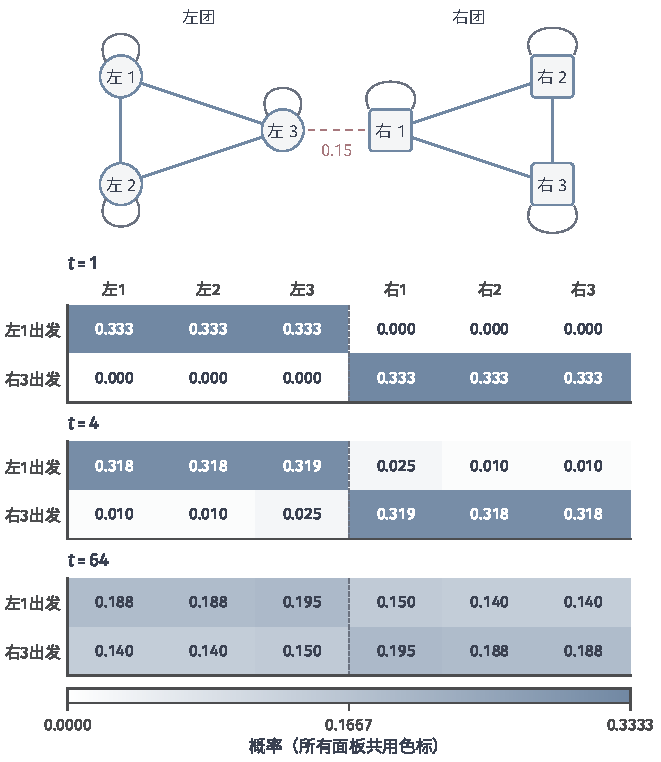
\includegraphics[width=105.412mm]{figures/03-models/01-classic-models/matplotlib/dim-diffusion-walk/figure.pdf}
  \caption{扩散时间与跨团瓶颈。每团三个节点，团内边及所有自环权重为1，唯一跨团边权重为$0.15$。令$\alpha=0$并按行归一化，热图两行分别表示从左1、右3出发的$\bm{P}^t$对应行，六列为固定节点顺序；各时刻共用同一连续概率色标。数值由有理数矩阵乘法计算，显示三位小数，舍入后行和可能略偏离1。64步仍未充分混合；因图连通且有自环，极限分布均为$\bm{\pi}^{\top}=(20,20,21,21,20,20)/122$。}
  \label{fig:dim-diffusion-walk}
\end{figure}

\subsubsection{参数学习}

记$\bm{\Pi}=\operatorname{diag}(\pi_1,\ldots,\pi_n)$。由细致平衡，矩阵
\[
  \bm{S}=\bm{\Pi}^{1/2}\bm{P}\bm{\Pi}^{-1/2}
\]
为对称矩阵。取其欧氏单位特征向量$\bm{u}_\ell$，并令$\bm{\psi}_\ell=\bm{\Pi}^{-1/2}\bm{u}_\ell$，则
\begin{equation}
  \label{eq:dim-diffusion-eigenvectors}
  \begin{aligned}
    \bm{P}\bm{\psi}_\ell&=\lambda_\ell\bm{\psi}_\ell,\\
    \sum_i\pi_i\psi_\ell(i)\psi_r(i)&=\delta_{\ell,r}.
  \end{aligned}
\end{equation}
这些特征函数在$L^2(\bm{\pi})$内积下正交。连通图的常数特征对为$\lambda_0=1,\psi_0(i)=1$，其余特征值在$[-1,1]$内。再满足非周期性时，非平凡特征值的绝对值小于一。连通图保留正自环即可保证非周期性，无自环二部图却可能出现$-1$特征值。

非负对称权重仍可能有负特征值，应按$|\lambda_1|\geq|\lambda_2|\geq\cdots$选择扩散模态。全连接半正定核经对角缩放仍半正定，此时才可按非负特征值降序选取；稀疏截断可能破坏半正定性。$k$维扩散坐标定义为
\begin{equation}
  \label{eq:dim-diffusion-map}
  \bm{\Psi}_{t,k}(i)
  =\bigl(\lambda_1^t\psi_1(i),\ldots,
         \lambda_k^t\psi_k(i)\bigr)^{\top}.
\end{equation}
将这些坐标按行放置，得到$n\times k$矩阵。$t$对应转移矩阵的整数幂；含负特征值时，直接令$t$取任意实数将失去这一解释。

稠密矩阵的构造、存储及完整谱分解成本与核PCA同阶。稀疏权重降低矩阵向量乘成本，总求谱时间仍受$k$、谱间隔及精度影响。除邻域或带宽与$k$外，还要选择$\alpha$和$t$；同一组谱可在不同$t$下重新加权，无需重复分解。

\subsubsection{理论分析}
\label{sec:dim-diffusion-theory}

\paragraph{表达能力}
扩散时间选择几何尺度，输出维数决定保留多少转移模态。坐标拟合的是给定核及归一化对应的扩散距离；原空间的其他距离可能改变。

谱表示在有限图上就成立。先求其精确关系与截断界，再讨论采样极限，可以分别判断代数近似与几何近似。

全部非平凡模态精确表示扩散距离，未保留的谱及平稳概率共同控制截断误差。下面在$L^2(\bm{\pi})$中展开转移概率，用正交性消去交叉项；核尺度与有限图的结构误差仍需另行检查。

\begin{theorem}[扩散距离的谱表示与截断界]
  \label{thm:dim-diffusion-isometry}
  设$\bm{P}$由连通的对称非负权重构造，$\pi_i>0$，特征函数按式\eqref{eq:dim-diffusion-eigenvectors}归一化。对整数$t\geq0$，全部非平凡模态给出
  \begin{equation}
    \label{eq:dim-diffusion-identity}
    D_t^2(i,j)
    =\sum_{\ell=1}^{n-1}\lambda_\ell^{2t}
      \bigl(\psi_\ell(i)-\psi_\ell(j)\bigr)^2.
  \end{equation}
  当$t=0$时按$\bm{P}^0=\bm{I}_n$约定所有模态系数为一。若按特征值绝对值排序，$k<n-1$且$i\ne j$，截断的平方距离误差$R_{t,k}$满足
  \begin{equation}
    \label{eq:dim-diffusion-tail}
    \begin{aligned}
      R_{t,k}(i,j)
        &:=D_t^2(i,j)
          -\lVert\bm{\Psi}_{t,k}(i)-\bm{\Psi}_{t,k}(j)\rVert_2^2,\\
      0\leq R_{t,k}(i,j)
        &\leq|\lambda_{k+1}|^{2t}
          \left(\frac1{\pi_i}+\frac1{\pi_j}\right).
    \end{aligned}
  \end{equation}
\end{theorem}
\begin{proof}
  对称矩阵$\bm{S}$的谱分解给出
  \[
    p_t(i,a)=\pi_a\sum_{\ell=0}^{n-1}
      \lambda_\ell^t\psi_\ell(i)\psi_\ell(a).
  \]
  令$c_\ell=\lambda_\ell^t(\psi_\ell(i)-\psi_\ell(j))$，则$c_0=0$。代入定义，展开平方并使用加权正交性：
  \[
    \begin{aligned}
      D_t^2(i,j)
        &=\sum_a\pi_a
          \left(\sum_{\ell=1}^{n-1}c_\ell\psi_\ell(a)\right)^2\\
        &=\sum_{\ell,r=1}^{n-1}c_\ell c_r
          \sum_a\pi_a\psi_\ell(a)\psi_r(a)
         =\sum_{\ell=1}^{n-1}c_\ell^2.
    \end{aligned}
  \]
  其中$\pi_a$来自分子中$\pi_a^2$除以定义中的$\pi_a$，不能再次消去。截断后余项是$\ell>k$的非负和。由绝对值排序及完整正交基关系，
  \[
    \begin{aligned}
      R_{t,k}
        &\leq|\lambda_{k+1}|^{2t}
          \sum_{\ell=1}^{n-1}
            (\psi_\ell(i)-\psi_\ell(j))^2,\\
      \sum_{\ell=0}^{n-1}\psi_\ell(i)\psi_\ell(j)
        &=\frac{\delta_{i,j}}{\sqrt{\pi_i\pi_j}},
    \end{aligned}
  \]
  对$i\ne j$展开平方，即得所述上界；$i=j$时两种距离和余项都为零。
\end{proof}

保留全部$n-1$个模态时距离精确，截取$k$维则一般有误差。式\eqref{eq:dim-diffusion-tail}同时含谱尾部与平稳概率，稀少区域可能有更大的绝对误差界。增大时间虽使该界缩小，真实扩散距离也随之缩小，不能据此保证相对精度改善。

不可约且非周期的有限链满足$|\lambda_\ell|<1$，故$t\to\infty$时，各起点的到达分布趋于$\bm{\pi}^{\top}$，距离也趋于零。混合前的较大$t$突出慢模态，过大的$t$则丢失区分。连续时间可另用$\exp[-s(\bm{I}_n-\bm{P})]$，以$e^{-s(1-\lambda_\ell)}$加权。

使用同一组对称权重时，拉普拉斯广义问题与转移矩阵满足
\[
  (\bm{D}_b-\bm{W})\bm{v}=\mu\bm{D}_b\bm{v}
  \quad\Longleftrightarrow\quad
  \bm{P}\bm{v}=(1-\mu)\bm{v}.
\]
两者因而共享特征方向。将选定模态的时间权重设为一，并调整归一化，可得到无时间加权的拉普拉斯坐标；$L^2(\bm{\pi})$与$\bm{D}_b$的归一化还差全局尺度。负谱存在时，按绝对值排序的扩散映射可能选中拉普拉斯高端模态，这一选择也需计入比较。

\paragraph{收敛性}
固定满足细致平衡的转移矩阵后，扩散坐标由谱分解求得。残差决定数值精度，谱分离和求解器影响迭代速度。游走时间$t$选择表示尺度，与求谱算法的迭代次数分别控制不同问题。

\paragraph{泛化性}

密度修正要在采样极限中解释。在光滑正密度$p$、足够采样及小高斯带宽的内点极限下，生成元含有与$2(1-\alpha)\nabla_{\mathcal{M}}\log p$有关的漂移。$\alpha=1$消去主导密度漂移，使极限扩散由流形几何决定；有限样本仍可能有密度影响。$\alpha=0$保留密度作用，适用于任务本身关注该概率结构的情形。

新点可用Nystr\"om方式延拓。沿用训练核及$r_j$，计算$r(\bm{x})=\sum_j\kappa(\bm{x},\bm{x}_j)$，按训练归一化构造$p(\bm{x},j)$。当$\lambda_\ell\ne0$时，有
\begin{equation}
  \label{eq:dim-diffusion-extension}
  \psi_\ell(\bm{x})
  =\frac1{\lambda_\ell}\sum_jp(\bm{x},j)\psi_\ell(j),
  \qquad
  z_\ell(\bm{x})=\lambda_\ell^t\psi_\ell(\bm{x}).
\end{equation}
该式固定训练度和谱，将特征方程延伸到新点。小特征值的倒数会放大误差，零特征值需其他处理。错误连接对传播的影响取决于它如何改变瓶颈，使用多条路径也不能保证减弱每一条错误边的作用。

\subsubsection{小结}

扩散映射将谱坐标的距离解释为到达分布的差异。重加权度确定平稳分布，特征函数在$L^2(\bm{\pi})$中归一化，时间因子控制模态强弱。$\alpha$重加权调整密度作用；扩散小波则用扩散算子的幂组织多尺度函数基\scite{dimCoifmanMaggioni2006}

向量扩散映射将局部方向的对齐也纳入传播，可研究切向量的一致性，因而还需估计局部坐标系。这些扩展共享多步传播，但仍受核尺度、采样误差、慢模态选择、混合时间与延拓稳定性限制。

\subsection{随机邻居嵌入（SNE）}
\label{sec:dim-sne}

固定距离在不同密度的区域可能对应不同邻域规模。Hinton与Roweis于2002年提出\term{随机邻居嵌入}（stochastic neighbor embedding，SNE），为每个样本建立选择邻居的概率分布，再要求低维表示复现该分布。“随机”指邻居选择的概率模型，坐标仍由优化求得。

原论文用bank的歧义说明表示的局限：河岸与金融是不同语境，单一位置可能难以同时容纳两组邻居。因此作者也讨论了同一对象具有多个位置的混合扩展\scite{dim-hinton2002sne}本节采用单位置形式；邻域分布定义之后，还需判断低维空间能否表达这些关系。

\subsubsection{模型结构}

以$i$为中心，用高斯核将距离转为选择邻居的条件概率：
\begin{equation}
  \label{eq:dim-sne-high}
  \begin{aligned}
    p_{j\mid i}
      &=\frac{\exp(-\delta_{i,j}^2/(2\sigma_i^2))}
      {\sum_{\ell\ne i}\exp(-\delta_{i,\ell}^2/(2\sigma_i^2))},
      \qquad j\ne i,\\
    p_{i\mid i}&=0,\qquad \sum_{j\ne i}p_{j\mid i}=1.
  \end{aligned}
\end{equation}
带宽$\sigma_i>0$决定局部尺度。小带宽将概率集中到近邻，大带宽使远点获得更多权重。两点距离虽对称，条件概率通常不对称，因为各中心的带宽及归一化分母不同。

\term{困惑度}（perplexity）将分布$P_i=(p_{j\mid i})_{j\ne i}$的熵转为有效邻居数，以此校准带宽。采用自然对数时定义
\begin{equation}
  \label{eq:dim-sne-perplexity}
  \begin{aligned}
    H(P_i)&=-\sum_{j\ne i}p_{j\mid i}\log p_{j\mid i},\\
    \operatorname{Perp}(P_i)&=\exp\!\bigl(H(P_i)\bigr).
  \end{aligned}
\end{equation}
概率在$q$个邻居上均匀分配时，困惑度为$q$。一般值可以非整数，未规定固定数量的非零邻居。熵若改用以$2$为底的对数，外层应改为$2^{H_2(P_i)}$。

带宽可根据目标困惑度$\tau$二分搜索。记$\beta_i=1/(2\sigma_i^2)$、$D_j=\delta_{i,j}^2$及$B_i=\sum_{j\ne i}\exp(-\beta_iD_j)$，则
\begin{equation}
  \label{eq:dim-sne-entropy-monotonicity}
  \begin{aligned}
    H(P_i)&=\log B_i+\beta_i\mathbb{E}_{P_i}[D],\\
    \frac{\mathrm{d}}{\mathrm{d}\beta_i}\mathbb{E}_{P_i}[D]
      &=-\operatorname{Var}_{P_i}(D),\\
    \frac{\mathrm{d}H(P_i)}{\mathrm{d}\beta_i}
      &=-\beta_i\operatorname{Var}_{P_i}(D)\leq 0.
  \end{aligned}
\end{equation}
困惑度随带宽单调不减；距离不全相等时严格递增。设并列最近邻有$h_i$个，带宽从零趋向无穷时，困惑度从$h_i$趋向$n-1$，故$\tau\in(h_i,n-1)$才对应唯一有限正带宽。所有距离相等时值恒为$n-1$，重复或并列距离也会限制可达目标。

达到相同困惑度时，稀疏区域通常需更大带宽，稠密区域需更小带宽，所以校准后的邻域分布未直接保留原始密度。可从$5$至$50$探索困惑度，并结合样本数与群体规模调整。预处理仍重要：无关特征改变输入距离后，带宽搜索也会使用这些距离。

低维核尺度固定，坐标通过以下目标学习：
\begin{equation}
  \label{eq:dim-sne-low-loss}
  \begin{aligned}
    q_{j\mid i}
      &=\frac{\exp(-r_{i,j}^2)}
      {\sum_{\ell\ne i}\exp(-r_{i,\ell}^2)},\qquad q_{i\mid i}=0,\\
    C_{\mathrm{SNE}}(\bm{Z})
      &=\sum_i\operatorname{KL}(P_i\Vert Q_i)\\
      &=\sum_i\sum_{j\ne i}p_{j\mid i}
        \log\frac{p_{j\mid i}}{q_{j\mid i}}.
  \end{aligned}
\end{equation}
这里$Q_i=(q_{j\mid i})_{j\ne i}$。核$\exp(-r^2)$与方差为$1/2$、标准差为$1/\sqrt{2}$的高斯密度具有相同形状；固定带宽也就规定坐标单位。共同带宽的改变可由坐标缩放吸收，但在固定带宽下缩放坐标会改变概率与目标。

较大的$p_{j\mid i}$使近邻错置受到较大惩罚：拉远这对点会增加$-\log q_{j\mid i}$。高维远点若挤在低维近处，也会占用归一化概率，减少真正近邻的份额，因而产生排斥作用。整体KL散度非负，单个求和项仍可为负。

\subsubsection{参数学习}

先由$\bm{X}$和$\tau$求带宽并固定$P_i$，再优化坐标。令$A_i=\sum_{\ell\ne i}\exp(-r_{i,\ell}^2)$，以$i$为中心的散度展开为
\begin{equation}
  \label{eq:dim-sne-anchor-loss}
  \begin{aligned}
    C_i&=\sum_{j\ne i}p_{j\mid i}\log p_{j\mid i}
      +\sum_{j\ne i}p_{j\mid i}r_{i,j}^2+\log A_i.
  \end{aligned}
\end{equation}
第一项为常数，第二项按邻居概率拉近点对，第三项反映归一化竞争。求导时必须同时包含后两项，才能得到吸引与排斥共同作用的更新。

$\bm{z}_i$既是$C_i$的中心，也是其他$C_j$的候选邻居。两种贡献分别为
\begin{equation}
  \label{eq:dim-sne-two-roles}
  \begin{aligned}
    \nabla_{\bm{z}_i}C_i
      &=2\sum_{j\ne i}(p_{j\mid i}-q_{j\mid i})
        (\bm{z}_i-\bm{z}_j),\\
    \nabla_{\bm{z}_i}C_j
      &=2(p_{i\mid j}-q_{i\mid j})
        (\bm{z}_i-\bm{z}_j),\qquad j\ne i.
  \end{aligned}
\end{equation}
两个负项分别来自$\log A_i$与$\log A_j$的导数；后者只有含$i$的核项随$\bm{z}_i$变化。将中心与邻居两种贡献相加，得到
\begin{equation}
  \label{eq:dim-sne-gradient}
  \begin{aligned}
    \nabla_{\bm{z}_i}C_{\mathrm{SNE}}
      &=2\sum_{j\ne i}
        \bigl[(p_{j\mid i}-q_{j\mid i})\\
      &\qquad +(p_{i\mid j}-q_{i\mid j})\bigr]
        (\bm{z}_i-\bm{z}_j).
  \end{aligned}
\end{equation}
系数为正时，负梯度更新将$i$拉向$j$；系数为负时将两点推开。因此力的方向由负梯度确定，且需合计两个有向残差，它们可能相互抵消。

用正学习率$\eta_t$作更新$\bm{Z}^{(t+1)}=\bm{Z}^{(t)}-\eta_t\nabla C_{\mathrm{SNE}}(\bm{Z}^{(t)})$，也可加入动量。原工作使用逐渐减弱的随机扰动改善布局，但未保证全局最优。小随机点云能打破全部坐标重合时的对称零梯度状态。

计算完整高维距离需$O(n^2d)$时间，保存概率需$O(n^2)$空间。输出维数固定时，每轮优化为$O(n^2)$。可结合目标值、梯度或位移判断数值进展，再检查近邻保留；数值停止变化只说明当前优化状态。

\subsubsection{理论分析}
\label{sec:dim-sne-theory}

\paragraph{表达能力}
SNE主要拟合邻域选择概率。输出维数可能不足以同时表达全部关系，远处位置和簇间间距也未受到定量保真的约束。

\term{拥挤问题}（crowding problem）来自高维邻域与低维空间容量的差异。局部均匀采样于$m$维流形、尺度足够小且远离边界时，半径$r$内样本数近似随$r^m$增长，$k$维体积则随$r^k$增长。这里用的是内在维数$m$；这一比较提供直觉，实际计数还依赖数据与尺度。

$m>k$时，许多中距离关系可能争夺有限位置，高斯核快速衰减进一步限制布局。图\ref{fig:dim-neighbor-tails}中，$r=3$时高斯核约为$0.00012$，Cauchy形核为$0.1$，后者在较远位置仍保留相似度。图中是核值，归一化后的概率还取决于其他点。

\begin{figure}[htbp]
  \centering
  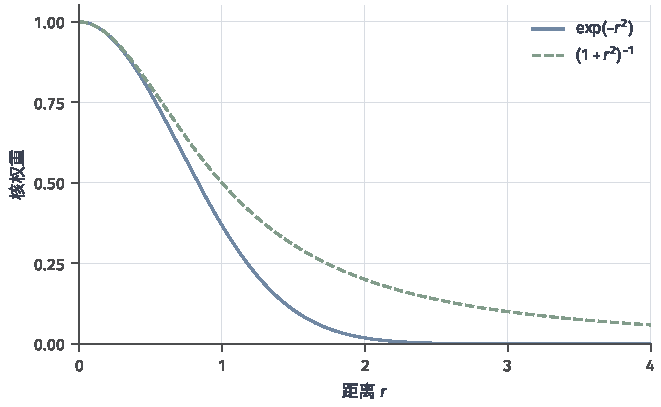
\includegraphics[width=105.412mm]{figures/03-models/01-classic-models/matplotlib/dim-neighbor-tails/figure.pdf}
  \caption{高斯核$\exp(-r^2)$与Cauchy形核$1/(1+r^2)$的尾部。横轴$r$为无量纲距离，纵轴为未归一化核值，非概率密度、非实验结果；尾部形状本身不保证嵌入保真。}
  \label{fig:dim-neighbor-tails}
\end{figure}

\paragraph{收敛性}
坐标目标非凸，平移、旋转和反射也使坐标解不唯一。梯度光滑且步长合适时，可研究下降与趋近驻点；任意初始化的全局收敛仍无保证。即使谱方法全局解出固定图的子问题，图是否表达真实几何也要另行判断。

\paragraph{泛化性}

标准SNE输出一组训练坐标。处理新样本需另定邻域及旧坐标是否固定，并检验表示稳定性。输入距离若主要来自噪声，充分优化也可能只是保留这些噪声关系。

\subsubsection{小结}

SNE先以困惑度校准邻域，再以条件概率和KL散度学习坐标。表示能力、布局优化和点对计算各有约束：更换核、改进优化与计算加速分别解决不同问题，需要分别评价。

\subsection{t-SNE}
\label{sec:dim-tsne}

重尾核使较远位置仍保有相似度，为拥挤邻域提供更多布局余地。van der Maaten与Hinton于2008年提出\term{t-SNE}（t-distributed stochastic neighbor embedding），同时将逐点条件分布改为对称点对分布\scite{dim-vandermaaten2008tsne}这两项改变共同定义其目标。

\subsubsection{模型结构}

沿用高维条件概率与困惑度，为每对样本构造一个对称权重：
\begin{equation}
  \label{eq:dim-tsne-joint}
  \begin{aligned}
    p_{i,j}&=\frac{p_{j\mid i}+p_{i\mid j}}{2n},\qquad i\ne j,\\
    p_{i,i}&=0,\qquad p_{i,j}=p_{j,i},\qquad
      \sum_{i\ne j}p_{i,j}=1.
  \end{aligned}
\end{equation}
求和包括有序对的两个方向。$n$个条件分布各归一化为$1$，两方向相加后的总和为$2n$，因此分母取$2n$。若改按$i<j$求和，归一化及后续导数系数也需调整。

低维点对采用Cauchy形核，并在全部有序对上归一化：
\begin{equation}
  \label{eq:dim-tsne-low}
  \begin{aligned}
    u_{i,j}&=(1+r_{i,j}^2)^{-1},\qquad
      \mathcal{Z}=\sum_{a\ne b}u_{a,b},\\
    q_{i,j}&=\frac{u_{i,j}}{\mathcal{Z}},\qquad i\ne j,\\
    q_{i,i}&=0,\qquad \sum_{i\ne j}q_{i,j}=1.
  \end{aligned}
\end{equation}
$u_{i,j}$具有自由度为$1$的一维Student $t$核形状，$q_{i,j}$则是有限点对上的离散概率。重尾允许较远点获得相似度，未规定高低维距离相等，也未将$q_{i,j}$定义为$\mathbb{R}^k$上的多元Cauchy密度。

记$\bm{P}=(p_{i,j})$、$\bm{Q}=(q_{i,j})$，以点对分布间的KL散度学习坐标：
\begin{equation}
  \label{eq:dim-tsne-loss}
  C_{\mathrm{tSNE}}(\bm{Z})
    =\sum_{i\ne j}p_{i,j}\log\frac{p_{i,j}}{q_{i,j}}.
\end{equation}
全部点对共享归一化常数$\mathcal{Z}$。移动一个点会改变它和其他点的核值，也改变其余点对的概率，所以坐标要在共同概率预算下协调。

高概率近邻错置受到较大惩罚，簇间距离、面积和密度却未被要求复原。小$p_{i,j}$的吸引弱，但这些点对仍参与归一化与斥力计算，局部目标也需要考虑远点。

\subsubsection{参数学习}

代入低维核并利用$\sum_{i\ne j}p_{i,j}=1$，展开目标与归一化项的梯度：
\begin{equation}
  \label{eq:dim-tsne-gradient-derivation}
  \begin{aligned}
    C_{\mathrm{tSNE}}
      &=\text{常数}
        +\sum_{a\ne b}p_{a,b}\log(1+r_{a,b}^2)
        +\log\mathcal{Z},\\
    \nabla_{\bm{z}_i}\mathcal{Z}
      &=-4\sum_{j\ne i}u_{i,j}^2(\bm{z}_i-\bm{z}_j),\\
    \nabla_{\bm{z}_i}\log\mathcal{Z}
      &=-4\sum_{j\ne i}q_{i,j}u_{i,j}(\bm{z}_i-\bm{z}_j).
  \end{aligned}
\end{equation}
距离平方的导数贡献因子$2$，有序对的两个方向再贡献因子$2$。吸引项同理给出$4\sum_{j\ne i}p_{i,j}u_{i,j}(\bm{z}_i-\bm{z}_j)$，因此
\begin{equation}
  \label{eq:dim-tsne-gradient}
  \nabla_{\bm{z}_i}C_{\mathrm{tSNE}}
    =4\sum_{j\ne i}(p_{i,j}-q_{i,j})u_{i,j}
      (\bm{z}_i-\bm{z}_j).
\end{equation}
$p_{i,j}>q_{i,j}$时，负梯度拉近点对，反之推开。即使稀疏近似中$p_{i,j}=0$，有限距离的$q_{i,j}$仍为正，因而仍有斥力。每个点的位移由全部点对作用合成。

\term{早期夸大}（early exaggeration）在初始阶段将梯度中的$p_{i,j}$乘以$\alpha>1$，增强吸引后再恢复$\alpha=1$。原文使用$4$，后续也常用$12$，但需与学习率及样本数配合。夸大后权重和为$\alpha$，该阶段的更新已不是原归一化分布间KL散度的梯度。

初始化和动量也影响优化。缩放后的PCA坐标提供结构化起点，随机点云则不带这一信息；因此宏观布局差异可能同时来自起点与目标。动量未保证逃离局部极小值。实验应记录困惑度、学习率、初始化和夸大系数及轮数。

原始算法每轮需$O(n^2)$计算。Barnes--Hut t-SNE将吸引图稀疏化，并用低维树聚合远点、近似斥力，二维常用四叉树。固定近邻预算及近似精度、输出维数较小时，每轮典型成本为$O(n\log n)$；建图及极端布局仍会影响时间\scite{dim-vandermaaten2014accelerating}

FIt-SNE通过网格插值和快速傅里叶变换加速核求和\scite{dim-linderman2019fitsne}固定插值阶数时，斥力成本约为$O(n+g\log g)$，其中$g$为网格节点数，此外还需计算稀疏吸引。范围与精度改变时$g$也会改变。2019年工作展示了百万级单细胞数据的处理，实际规模与收益仍依赖计算条件。

\subsubsection{理论分析}
\label{sec:dim-tsne-theory}

\paragraph{表达能力}
重尾核缓解部分局部拥挤，输出维数和点对概率目标仍限制表示。视觉上分离的簇可能来自该目标的布局，原空间未必具有相同间距或密度。

\paragraph{收敛性}

坐标目标仍非凸。Linderman与Steinerberger在2019年SIAM期刊论文中，针对有适当簇结构的输入相似度、集中初始点云及满足条件的步长和夸大系数，分析早期簇内收缩与谱聚类的联系\scite{dim-linderman2019clustering}结论针对该阶段和条件，未覆盖任意数据的整个训练。

初始间距小时，$u_{i,j}\approx1$。若斥力扰动相对较小并暂不计动量，更新近似为
\begin{equation}
  \label{eq:dim-tsne-spectral-approximation}
  \begin{aligned}
    \bm{Z}^{(t+1)}
      &\approx(\bm{I}-4\eta_t\alpha\bm{L}_{P})\bm{Z}^{(t)},\\
    \bm{L}_{P}&=\bm{D}_{P}-\bm{P},\qquad
    (\bm{D}_{P})_{i,i}=\sum_{j\ne i}p_{i,j}.
  \end{aligned}
\end{equation}
对角矩阵$\bm{D}_{P}$记录行和。步长合适时，图平滑抑制快速变化方向，因而与拉普拉斯谱相联系。点云展开后，核值接近$1$的近似会减弱，斥力也更不可忽略；关闭夸大后，布局仍由两种作用共同调整。

\paragraph{泛化性}

困惑度决定输入分布，也决定所求问题。小值强调细邻域，可能割裂连续结构；大值引入更广关系，可能模糊稀有群体。可在可达范围内比较$5$、$30$、$50$等尺度及多次初始化，寻找稳定关系。不同困惑度对应不同目标分布，其KL值不能直接用于排名。

旋转和镜像通常不改变解释，簇间距、面积及疏密却也不能直接换算为原空间量。布局可能展开大簇、压紧小簇，或将连续变化分成区域。单细胞、文本或图像特征中的分组应回到合适的高维表示验证，并分别考察内部指标、稳定性、参考标签及下游效果（参见第\ref{sec:clustering-summary}节）。

新点需要额外扩展规则。openTSNE等实现固定参考坐标，再按新点与参考样本的相似度优化新坐标\scite{dim-policar2024opentsne}这是条件定位，与新旧样本联合训练不同；参考集未覆盖的新群体可能被安排到失真位置。

需要反复处理新样本时，可令$\bm{z}_i=f_{\bm{\theta}}(\bm{x}_i)$，按邻域目标学习共享参数。van der Maaten于2009年提出参数化t-SNE，以前向计算表示新点\scite{dim-vandermaaten2009parametric}网络函数族限制可实现布局，批次构造与归一化也影响训练关系。

\subsubsection{小结}

t-SNE用对称点对分布和重尾核组织局部相似性，适合探索邻域，却未建立全局距离的定量地图。加速算法降低计算成本，扩展规则方便定位新点；表示、优化与结构保真的限制仍需分别判断。

\subsection{UMAP}
\label{sec:dim-umap}

邻接关系也可以逐边赋予强度，无需使全部点对权重和为一。\term{统一流形逼近与投影}（uniform manifold approximation and projection，UMAP）先合并局部加权图，再优化低维连接强度。

McInnes、Healy与Melville自2018年公开的方法长文，将拉普拉斯特征映射、黎曼几何与模糊拓扑联系起来，讨论非均匀样本的局部度量及其合并\scite{dim-mcinnes2018umap}这一构造也面向较高维预处理。方法长文与同年JOSS软件论文分别描述理论构造和实现，几何解释、实现行为与可视化效果应各自评价。

\subsubsection{模型结构}

以$N_q(i)$表示不含$i$的$q$个近邻。先取互异样本、无并列最近邻及单位局部连接设置。记$\rho_i=\min_{j\ne i}\delta_{i,j}$，定义有向权重
\begin{equation}
  \label{eq:dim-umap-directed}
  \begin{aligned}
    v_{j\mid i}
      &=
      \begin{cases}
        \exp\!\left(-\dfrac{\max(0,\delta_{i,j}-\rho_i)}
        {\sigma_i}\right),&j\in N_q(i),\\
        0,&j\notin N_q(i),
      \end{cases}\\
    \sum_{j\in N_q(i)}v_{j\mid i}&=\log_2 q.
  \end{aligned}
\end{equation}
偏移$\rho_i$使最近邻权重为$1$，带宽$\sigma_i$控制其余边衰减。上述条件下，$q>2$时权重和随带宽从$1$趋向$q$，可搜索满足目标的带宽。距离可按任务更换，相应的几何解释也需要调整。

这些值是边的隶属强度，多条边可同时很强。校准目标$\log_2 q$未将行和设为$1$，也未使用熵或困惑度。重复或并列样本、其他局部连接设置可能使多条边固定为$1$，导致目标不可达，因而实现还需处理零距离、带宽下界与容差。

用模糊并将两个方向合成对称权重：
\begin{equation}
  \label{eq:dim-umap-union}
  v_{i,j}=v_{j\mid i}+v_{i\mid j}-v_{j\mid i}v_{i\mid j}.
\end{equation}
所得$v_{i,j}=v_{j,i}\in[0,1]$。一方向为$1$则合并为$1$，两方向均为$0.4$则合并为$0.64$。这是模糊集合运算，无需把两条边假定为独立事件。

\term{模糊单纯集}（fuzzy simplicial set）将点、边和三角面等组合结构赋予隶属强度，提供局部描述的组合框架。实际目标主要使用样本与加权边，即一维骨架。有限图中的环和空白是否对应真实拓扑，仍需采样与几何证据。

低维边强度由可调重尾核给出：
\begin{equation}
  \label{eq:dim-umap-kernel}
  w_{i,j}=\frac{1}{1+a r_{i,j}^{2b}},\qquad a>0,\quad b>0.
\end{equation}
由\code{min\_dist}和\code{spread}选择$a,b$，使光滑核逼近近处接近$1$、超过指定尺度后衰减的曲线。\code{min\_dist}允许控制紧凑程度，未给每对点施加硬距离下界。$a=b=1$时核形与t-SNE的$u_{i,j}$相同，但没有全局归一化，因而与$q_{i,j}$不同。

将每条边视为带软标签的二元判断，就可以匹配高低维边强度。按无序对$i<j$写完整目标：
\begin{equation}
  \label{eq:dim-umap-bernoulli}
  \begin{aligned}
    C_{\mathrm{B}}(\bm{Z})
      &=\sum_{i<j}\left[
        v_{i,j}\log\frac{v_{i,j}}{w_{i,j}}\right.\\
      &\qquad\left.+
        (1-v_{i,j})\log\frac{1-v_{i,j}}{1-w_{i,j}}
        \right].
  \end{aligned}
\end{equation}
该式求和逐边Bernoulli分布的KL散度。去掉只依赖高维权重的常数，得到二元交叉熵：
\begin{equation}
  \label{eq:dim-umap-cross-entropy}
  \begin{aligned}
    C_{\mathrm{CE}}(\bm{Z})
      &=-\sum_{i<j}\left[
        v_{i,j}\log w_{i,j}\right.\\
      &\qquad\left.+
        (1-v_{i,j})\log(1-w_{i,j})\right].
  \end{aligned}
\end{equation}
采用$0\log0=0$。两式对坐标有相同梯度，所以与t-SNE的核心区别在匹配对象：这里逐边二元匹配，t-SNE匹配全局归一化的点对分布。

正边项吸引，非边项排斥。$v_{i,j}=0$只说明局部图未保留这条连接，未区分稍远与极远的点对，因此该目标未规定全局距离保真。

\subsubsection{参数学习}

记吸引损失$\ell^+_{i,j}=-\log w_{i,j}$、排斥损失$\ell^-_{i,j}=-\log(1-w_{i,j})$。点对距离$r_{i,j}>0$时，其梯度为
\begin{equation}
  \label{eq:dim-umap-pair-gradient}
  \begin{aligned}
    \nabla_{\bm{z}_i}\ell^+_{i,j}
      &=\frac{2ab r_{i,j}^{2b-2}}
        {1+a r_{i,j}^{2b}}(\bm{z}_i-\bm{z}_j),\\
    \nabla_{\bm{z}_i}\ell^-_{i,j}
      &=-\frac{2b}
        {r_{i,j}^2(1+a r_{i,j}^{2b})}
        (\bm{z}_i-\bm{z}_j).
  \end{aligned}
\end{equation}
两项负梯度分别拉近与推开点对，完整目标再按$v_{i,j}$与$1-v_{i,j}$加权。接近重合时排斥项奇异，计算需稳定处理并控制更新幅度。

全点对计算仍为二次规模。\term{负采样}（negative sampling）按正边权重安排吸引，再为中心点抽$s$个排斥对象，抽样未逐个检查它们是否为非邻居。若图有$O(nq)$条边，每边每轮更新次数有界、$k$固定，一轮约需$O(nq(1+s))$；近似线性还要求$q,s$固定，并未包含建图和总轮数。

中心的更新频率取决于正边权重，负样本频率取决于采样分布。缺少重要性修正时，期望更新一般不同于完整交叉熵梯度，吸引与排斥的相对强度也随之改变。

Damrich与Hamprecht于2021年分析有效更新。令$\omega_i=\sum_{j\ne i}v_{i,j}$。在均匀负采样且排斥更新双端的模型下，略去共同正常数，有效目标为
\begin{equation}
  \label{eq:dim-umap-effective-loss}
  \begin{aligned}
    \widetilde C(\bm{Z})
      &=\sum_{i<j}\left[
        v_{i,j}\ell^+_{i,j}
        +\gamma_{i,j}\ell^-_{i,j}\right],\\
    \gamma_{i,j}&=\frac{s(\omega_i+\omega_j)}{2n}.
  \end{aligned}
\end{equation}
排斥系数由样本数、加权度和采样数决定，已不同于$1-v_{i,j}$。原文分析的非参数实现只移动排斥对的一端，其期望更新一般甚至没有对应的标量损失；上式仅适用于补上双端更新的版本\scite{dim-damrich2021umaploss}

暂将各$w_{i,j}$视为独立变量，其最优值为$v_{i,j}/(v_{i,j}+\gamma_{i,j})$。正边权重远大于排斥系数时，该值接近$1$，解释了部分紧凑布局倾向。实际坐标耦合全部边强度，未必能同时达到这些逐边最优值。

实现先搜近邻、估计尺度、合并图，再初始化并作采样更新。可取谱或随机初始化；断连分量之间缺少相对位置约束。学习率衰减、负样本数和排斥强度也影响布局，需与主要参数一起记录。

\code{n\_neighbors}控制连接尺度，较大值加入更广关系。\code{min\_dist}小允许紧凑群组，大则通常更分散，但这些变化未保证评价指标单调改善。\code{umap-learn}常用$q=15$、\code{min\_dist=0.1}作为起点；还需记录度量、维数、轮数、种子及版本\scite{dim-mcinnes2018umapsoftware}

\subsubsection{理论分析}
\label{sec:dim-umap-theory}

\paragraph{表达能力}
邻域图与距离约定选择关系尺度，输出维数限制可表达的连接强度。局部关系的近似匹配未要求全局等距，也未保证表示可逆或唯一。

\paragraph{收敛性}

完整交叉熵及有效采样目标都对坐标非凸，近邻近似、有限轮更新和梯度裁剪还会改变求解行为。趋近驻点的条件结论仅涉及给定目标，未保证最佳拓扑布局。负采样分析解释有效吸引与排斥，也未建立与非负矩阵分解的等价或相对t-SNE的普遍优势。

\paragraph{泛化性}

局部流形、尺度调整和模糊拼接说明图如何构造。有限样本结果仍依赖光滑几何、合适度量与足够采样；理论构造、近似建图和采样求解各有条件，不能直接将一层的保证用于另一层。

\code{transform}先在训练集找新点邻居，以邻居坐标初始化，再固定参考表示优化新点。这是给定参考图的条件定位。新数据接近训练分布时可借此放入同一图；新类别或分布漂移却可能使位置失真。

共享输入函数提供另一种扩展。Sainburg、McInnes与Gentner的参数化UMAP以正负样本训练网络，支持小批次和半监督学习\scite{dim-sainburg2021parametricumap}它通过前向计算处理新点，与固定参考图后优化位置不同；分布外泛化及对非参数布局的复现仍需验证。

子样本拟合后变换其余点可以节省计算，但子样本要覆盖稀有群体等重要关系。用于预测时，只在训练划分内拟合预处理和嵌入，再变换验证、测试数据，以免结构泄漏。表示的预测效用需直接评价。

\subsubsection{小结}

UMAP通过局部尺度与模糊并构图，以可调核布局并用采样降低计算量。边强度、完整匹配目标和有效更新各有含义。度量、建图、初始化及采样共同影响参考图与新点位置，应结合实际任务判断结果。

\subsection{模型对比与总结}
\label{sec:dim-manifold-comparison}
\label{sec:dim-neighbors-comparison}

表\ref{tab:dim-manifold-comparison}按输入、保留对象与求解比较六种方法。关系数据可以用于这些模型，但流形假设和谱求解并非共同前提：应力MDS通常迭代拟合。复杂度也应结合稠密矩阵、稀疏图或具体近似方案说明。

\begin{table*}[htbp]
  \centering
  \small
  \begin{tabularx}{\linewidth}{@{}>{\RaggedRight\arraybackslash}p{22mm}>{\RaggedRight\arraybackslash}X>{\RaggedRight\arraybackslash}X>{\RaggedRight\arraybackslash}X@{}}
    \toprule
    方法 & 输入与保留对象 & 核心求解 & 样本外使用与主要限制 \\
    \midrule
    MDS & 给定差异；经典型拟合内积，应力型拟合距离或顺序
      & 经典型取正谱；度量及非度量应力通常迭代求解
      & 需要到训练点的差异；非欧氏性与目标维数限制保真程度 \\
    核PCA & 正定核；特征空间方差
      & 中心化核矩阵的主特征方向
      & 核投影有明确公式；依赖训练中心化、核尺度和谱隙 \\
    Isomap & 邻域图；全局测地距离的估计
      & 最短路径后做经典MDS
      & 接入图后做距离扩展；短路、断连及不可展开几何会失真 \\
    LLE & 邻居与局部重构权；仿射重构关系
      & 局部线性方程与全局低端谱
      & 局部权重插值；病态邻域、多零模态与噪声需诊断 \\
    Laplacian Eigenmaps & 对称非负邻域权重；图上平滑性
      & 度加权广义特征值问题
      & 可作谱延拓；度、密度、断连影响低频表示 \\
    Diffusion Map & 对称权重及重加权；给定步数的扩散距离
      & 满足细致平衡的转移矩阵谱与时间加权
      & Nystr\"om延拓；截断、带宽和过度混合限制区分能力 \\
    \bottomrule
  \end{tabularx}
  \caption{六类方法在本节所述标准构造下的比较。MDS一行区分经典型与应力型，不能把二者的目标和求解混同。样本外一栏均指固定训练表示后的扩展，不代表加入新样本重新训练的等价结果，也不是预测性能保证。}
  \label{tab:dim-manifold-comparison}
\end{table*}

选择始于可信关系及误差含义。感知差异可用MDS，核PCA保留特征空间方差，Isomap适合有意义且可展开的长度结构。可信仿射关系对应LLE，图平滑对应拉普拉斯坐标，跨尺度概率连通对应扩散距离。分析动力系统时，还需让构图对应所研究的过程，才能将慢模态解释为相关慢变量。

\term{Hessian LLE}（Hessian特征映射）估计局部坐标函数的二阶变化，寻找其平方积分接近零的方向。连通且局部等距于欧氏区域等条件下，仿射坐标的Hessian为零；原理论允许某些非凸、带孔参数区域，但未涵盖任意带孔流形。估计二阶项还需足够且分布合适的邻居，采样要求通常比一阶拟合更强\scite{dimDonoho2003}

\term{局部切空间对齐}（local tangent space alignment, LTSA）在邻域中用PCA估计$m$维切空间及局部坐标，再令全局坐标经各邻域的仿射变换与其对齐。它显式利用局部线性结构，切空间估计与邻域选择的误差也会传到全局\scite{dimZhang2004}

\term{最大方差展开}（maximum variance unfolding, MVU）直接约束局部距离，优化未知Gram矩阵$\bm{B}$：
\[
  \begin{aligned}
    \max_{\bm{B}\succeq0}\quad&
      \operatorname{tr}(\bm{B}),\qquad \bm{B}\bm{1}=\bm{0},\\
    \text{满足}\quad&
      \bm{B}_{i,i}+\bm{B}_{j,j}-2\bm{B}_{i,j}
      =\lVert\bm{x}_i-\bm{x}_j\rVert_2^2,\quad(i,j)\in E.
  \end{aligned}
\]
中心化时，增大迹就是在保持局部边长下增大总方差。Gram矩阵上的问题是凸半正定规划，若再指定秩为$k$，则失去一般凸性。原问题的最优秩未必为$k$，截断后也可能违反局部距离约束；半正定求解本身还限制规模\scite{dimWeinberger2006}

\term{向量扩散映射}（vector diffusion maps）用邻域切空间间的正交对齐矩阵，使路径上的方向运输参与传播\scite{dimSinger2012}其连续对象是作用于向量场的连接拉普拉斯，补充了标量扩散没有直接表达的方向一致性。是否有益取决于任务所需信息。

这些方法各自约束不同对象。GPLVM用潜变量到观测的概率映射与似然学习坐标，t-SNE和UMAP用邻域目标布局，均不能一般化为给距离做经典MDS。概率邻域法与几何方法也分别适合不同目的，应按目标解释视觉分离与簇间位置。

非线性降维需要先选择可信关系，再判断目标维数能保留多少。核、邻域、归一化与时间尺度改变关系本身；求解正确、训练误差小、流形极限存在和下游有效，是四项需要分别核验的结果。

表\ref{tab:dim-neighbors-comparison}归纳三种邻域法的目标与边界。t-SNE困惑度为有效邻居数，UMAP的$q$为建图邻居数，两者均控制尺度，却不能直接换算。

\begin{table*}[tbp]
  \centering
  \small
  \begin{tabularx}{\linewidth}{@{}p{0.13\linewidth}>{\RaggedRight\arraybackslash}X>{\RaggedRight\arraybackslash}X>{\RaggedRight\arraybackslash}X@{}}
    \toprule
    比较方面 & SNE & t-SNE & UMAP \\
    \midrule
    高维对象 & 逐点条件邻居概率 & 对称联合点对概率 & 稀疏模糊邻域图权重 \\
    低维对象 & 行归一化高斯核 & 全局归一化重尾核 & 不作概率归一化的可调重尾权重 \\
    建模依据 & 条件分布匹配 & 点对分布匹配 & 局部几何与模糊图构造 \\
    优化目标 & 条件KL散度之和 & 联合KL散度 & 逐边交叉熵；负采样改变有效目标 \\
    邻域尺度 & 困惑度及逐点带宽 & 困惑度及逐点带宽 & 邻居数$q$、局部距离偏移和带宽 \\
    布局控制 & 初始化、学习率等 & 初始化、夸大、学习率等 & 初始化、核形状、采样和排斥等 \\
    迭代代价 & 稠密计算$O(n^2)$ & 稠密$O(n^2)$；树或插值可加速 & 固定嵌入维数下约$O(nq(1+s))$ \\
    全局解释 & 不保证距离或密度保真 & 簇间距、面积不宜直接解释 & 图连接提供约束，但不保证全局保真 \\
    收敛边界 & 非凸、依赖初始化 & 非凸；部分早期阶段有条件分析 & 非凸；依赖实际采样更新规则 \\
    新样本 & 需另定义扩展 & 参考图扩展或参数化版本 & \code{transform}或参数化版本 \\
    \bottomrule
  \end{tabularx}
  \caption{三种邻域降维方法。复杂度指固定嵌入维数下的一轮优化，不含建图和总轮数；$s$为每次正边更新的负采样数。}
  \label{tab:dim-neighbors-comparison}
\end{table*}

比较速度时应固定近邻搜索、近似精度、硬件、线程及优化预算，才能解释差异。预处理、初始化、版本与并行方式也影响复现。固定种子便于重跑，多种子和多尺度则用于检查结构稳定性。

% 将段落与其完整的会议文献边注安排在同一页内。
\Needspace{9\baselineskip}
LargeVis将可扩展建图与布局结合。Tang等人用随机投影树和邻居探索得到近似近邻图，再用概率图布局及负采样优化吸引与排斥\scite{dim-tang2016largevis}其目标另有定义，未无偏求解原SNE的条件KL。

% PaCMAP的长标题与作者列表也需留出边注空间。
\Needspace{10\baselineskip}
PaCMAP增加群组间位置的约束。Wang等人在近邻和远点对之外采中距离对，按阶段调整其权重以组织较大尺度关系\scite{dim-wang2021pacmap}实际效果还取决于配对、损失及初始化，实验指标改善需在相应数据范围内解释。

% 为该段及其较长的边注引文保留共同的页内空间。
\Needspace{9\baselineskip}
Amid与Warmuth于2019年提出TriMap，以三元组$(i,j,\ell)$要求$j$比$\ell$更接近$i$，并通过跨尺度采样与加权损失组织这些相对关系\scite{dim-amid2019trimap}结果保留所选排序，三元组与起点仍影响布局。

流形学习与邻域嵌入共享部分局部建图思路，选择时宜比较约束量、近似方式与目标。测地关系可用Isomap考察，相似样本的组织可用t-SNE和UMAP探索。用于下游特征时还可取$k>2$，按任务评价选择维数。

邻域嵌入优先表示重要邻接关系，图形因而可用于提出假设或展示已有分析支持的结构。簇数、大小与间隔仍需在原始或合适的高维表示中检验，并结合尺度、初始化及领域知识判断。经过这些核验，视觉关系才可成为分析证据。

\section{基于概率的降维}
\label{sec:dim-probabilistic}

概率降维先规定低维因素如何生成观测，再用观测推断这些因素。PPCA、FA与GPLVM分别改变映射、噪声或未知量的处理方式，均沿用$n,d,k$及输入矩阵$\bm{X}$。这一生成视角与第\ref{sec:classic-overview-probabilistic}节的潜变量建模相联系。

\subsection{概率主成分分析（PPCA）与因子分析}
\label{sec:dim-ppca}

多个传感器测量共同状态，却各有读数误差。区分共同变化与噪声，可以更明确地解释低维表示。\term{概率主成分分析}（probabilistic principal component analysis, PPCA）以低维高斯状态生成线性信号，再叠加同方差高斯噪声。

允许各观测坐标有不同噪声方差，就得到高斯\term{因子分析}（factor analysis, FA）。“因子”表示解释共同变化的潜变量。历史可追溯到Spearman于1904年的一般智力研究，现代多因子模型的含义和范围已不同于当时的心理测量假说\scite{spearman1904intelligence}

Tipping与Bishop在1999年为PCA引入与因子分析相关的概率模型，以似然刻画主子空间并研究EM估计\scite{tipping1999}在同一似然下，谱解与潜变量迭代可以比较，噪声及缺失观测也可以纳入统计推断。

\subsubsection{模型结构}
\label{sec:dim-ppca-structure}

令$\bm{z}\in\mathbb{R}^k$为潜变量，$\bm{W}\in\mathbb{R}^{d\times k}$为载荷，$\bm{\mu}\in\mathbb{R}^d$为均值。PPCA取$1\leq k<d$，以独立的潜变量和噪声生成观测：
\begin{equation}
\label{eq:dim-ppca-generative}
\begin{aligned}
\bm{z}&\sim\mathcal{N}(\bm{0},\bm{I}_k),\\
\bm{x}&=\bm{\mu}+\bm{W}\bm{z}+\bm{\epsilon},\\
\bm{\epsilon}&\sim\mathcal{N}(\bm{0},\sigma^2\bm{I}_d),
\qquad \bm{\epsilon}\perp\bm{z},\quad \sigma^2>0.
\end{aligned}
\end{equation}
各向同性约束噪声方向，观测的总方差仍可不同。给定潜变量时，条件负对数似然含平方残差$\lVert\bm{x}-\bm{\mu}-\bm{W}\bm{z}\rVert_2^2/(2\sigma^2)$；拟合边缘似然则还要将潜变量积分掉。

图~\ref{fig:dim-latent-model}区分两个方向：生成时抽取潜变量并加噪声，编码时给定观测求潜变量后验。
\begin{figure}[htbp]
  \centering
  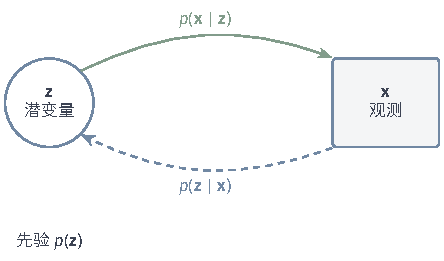
\includegraphics[width=75.188mm]{figures/03-models/01-classic-models/tikz/dim-latent-model/figure.pdf}
  \caption{概率生成与后验推断的结构示意。实线表示$\bm{z}\to\bm{x}$的生成方向；虚线表示$\bm{x}\to\bm{z}$的后验推断，不是额外的生成依赖。图中节点与箭头只说明变量角色和条件关系，不表示实测数据、网络层数或计算流程；噪声描述观测对信号的偏离，不是新增的潜变量维数。}
\label{fig:dim-latent-model}
\end{figure}

独立高斯量线性组合仍为高斯量，将潜变量积分后得到
\begin{equation}
\label{eq:dim-ppca-marginal}
\begin{aligned}
p(\bm{x})&=\mathcal{N}(\bm{x};\bm{\mu},\bm{C}),\\
\bm{C}&=\bm{W}\bm{W}^\top+\sigma^2\bm{I}_d.
\end{aligned}
\end{equation}
信号协方差的秩至多为$k$，正噪声使$\bm{C}$正定；样本不足导致经验协方差奇异时，模型协方差仍可正定。

FA将噪声改为$\bm{\Psi}=\operatorname{diag}(\psi_1,\ldots,\psi_d)$，其中$\psi_j>0$为方差，故$\bm{C}=\bm{W}\bm{W}^\top+\bm{\Psi}$。给定因子，各维条件独立，跨维协方差由共同因子产生。独特方差也可包含特征自身的变化，解释时需结合测量机制；标准化会同时改变同方差假设的含义。

图\ref{fig:dim-ppca-fa-noise}固定载荷，只比较条件噪声。给定一个潜变量值，PPCA允许观测沿各方向等幅偏离均值，FA允许沿某坐标偏离更多。圆与椭圆均表示条件噪声；再混合不同潜变量值，才会加入信号协方差并形成总体分布。

\begin{figure}[htbp]
  \centering
  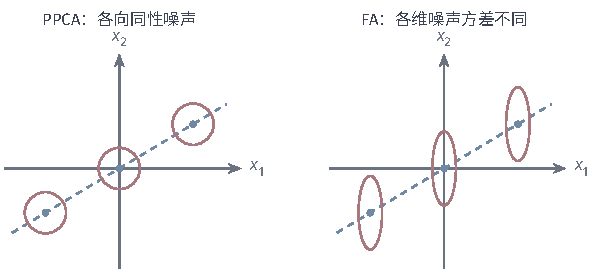
\includegraphics[width=101.840mm]{figures/03-models/01-classic-models/tikz/dim-ppca-fa-noise/figure.pdf}
  \caption{PPCA与FA的条件噪声示意。设$d=2$、$k=1$、$\bm{\mu}=\bm{0}$、$\bm{W}=(1,0.6)^\top$，三个实心点对应$z=-1,0,1$的条件均值。左图取$\sigma=0.28$，右图取$\bm{\Psi}=\operatorname{diag}(0.16^2,0.50^2)$；每条轮廓到其中心的平方Mahalanobis距离均为$1$。坐标为无量纲构造值，轮廓是条件等密度线，不是总体数据云或置信区域。}
  \label{fig:dim-ppca-fa-noise}
\end{figure}

载荷的正交旋转$\bm{W}\bm{R}$不改变协方差。载荷满列秩且除旋转外局部可识别时，可扣除$k(k-1)/2$个旋转自由度：PPCA与FA的协方差参数数目分别为$dk+1-k(k-1)/2$及$dk+d-k(k-1)/2$，均值另有$d$个。FA还需排除载荷与噪声间的额外歧义。相较自由协方差的$d(d+1)/2$个参数，低秩约束可以降低估计方差，也可能带来模型偏差。

\subsubsection{参数学习}
\label{sec:dim-ppca-learning}

设样本独立同分布，均值为$\bar{\bm{x}}$，中心化量为$\bm{y}_i=\bm{x}_i-\bar{\bm{x}}$，记$\bm{S}=n^{-1}\sum_i\bm{y}_i\bm{y}_i^\top$。固定$\bm{C}$时，均值梯度$n\bm{C}^{-1}(\bar{\bm{x}}-\bm{\mu})$与负定二阶导数给出$\hat{\bm{\mu}}=\bar{\bm{x}}$。代回最大似然目标得
\begin{equation}
\label{eq:dim-ppca-likelihood}
\ell=-\frac{n}{2}\left[
d\log(2\pi)+\log|\bm{C}|
+\operatorname{tr}(\bm{C}^{-1}\bm{S})\right].
\end{equation}
对数行列式惩罚过大的协方差体积，迹项则惩罚在数据有较大变化的方向上赋予过小方差。

对$\bm{S}$作谱分解$\bm{U}\bm{\Lambda}\bm{U}^\top$，按$\lambda_1\geq\cdots\geq\lambda_d\geq0$排列。令$\bm{U}_k$包含前$k$个方向，$\bm{\Lambda}_k=\operatorname{diag}(\lambda_1,\ldots,\lambda_k)$。

证明需要比较两组谱的配对。Birkhoff--von Neumann分解说明：行和、列和均为$1$的非负方阵，即双随机矩阵，可以写成置换矩阵的凸组合\scite{birkhoff1946}因此双随机矩阵上的线性目标至少为某个置换取值的最小值。

最大似然解以PCA主方向构造载荷，以舍弃特征值的均值估计噪声，载荷内部保留旋转自由。下面先证明样本谱与模型谱同序配对最优，再优化谱值，从而说明全局最优性；奇异点及高维统计保证仍需另外讨论。

\begin{theorem}[PPCA的最大似然解]
\label{thm:dim-ppca-mle}
设$1\leq k<d$，尾谱均值$\tau=(d-k)^{-1}\sum_{j=k+1}^d\lambda_j$满足$\tau>0$且$\lambda_k>\tau$。在$\sigma^2>0$的PPCA模型中，以下参数达到全局最大似然：
\begin{equation}
\label{eq:dim-ppca-mle}
\begin{aligned}
\hat{\bm{\mu}}&=\bar{\bm{x}},\qquad
\hat{\sigma}^2=\tau,\\
\hat{\bm{W}}&=\bm{U}_k(\bm{\Lambda}_k-\tau\bm{I}_k)^{1/2}\bm{R}.
\end{aligned}
\end{equation}
其中$\bm{R}$为任意$k$阶正交矩阵。截断处有重根时，$\bm{U}_k$可在对应特征子空间内选取不同正交方向。
\end{theorem}

\begin{proof}
需最小化$F(\bm{C})=\log|\bm{C}|+\operatorname{tr}(\bm{C}^{-1}\bm{S})$。写$s=\sigma^2$，由信号半正定且秩至多为$k$，可行协方差的谱满足
\[
c_1\geq\cdots\geq c_k\geq s,\qquad
c_{k+1}=\cdots=c_d=s>0.
\]
允许$c_j=s$便包括载荷秩不足$k$的情况。

固定谱，设$\bm{p}_b$为$\bm{C}$的第$b$个单位特征向量，则
\[
\operatorname{tr}(\bm{C}^{-1}\bm{S})
=\sum_{a=1}^d\sum_{b=1}^d
\frac{\lambda_a}{c_b}(\bm{u}_a^\top\bm{p}_b)^2.
\]
平方内积构成非负且各行各列和为$1$的双随机矩阵，可写成置换矩阵的凸组合，所以上式不小于置换配对的最小值。若$\lambda_a\geq\lambda_b$、$c_a\geq c_b$，同序配对减去交换配对等于
\[
(\lambda_a-\lambda_b)
\left(\frac{1}{c_a}-\frac{1}{c_b}\right)\leq0.
\]
消去逆序配对即得$\operatorname{tr}(\bm{C}^{-1}\bm{S})\geq\sum_j\lambda_j/c_j$，取$\bm{p}_j=\bm{u}_j$达到等号。对数行列式只依赖谱，故同序对齐是固定谱下的全局最优。

对齐后，目标化为
\[
\begin{aligned}
F&=\sum_{j=1}^k\left(\log c_j+\frac{\lambda_j}{c_j}\right)\\
&\quad+(d-k)\log s+\frac{(d-k)\tau}{s}.
\end{aligned}
\]
暂去$c_j\geq s$及排序约束。对$a>0$，函数$g_a(v)=\log v+a/v$的导数为$(v-a)/v^2$，在$a$左侧为负、右侧为正，故$v=a$为唯一全局最小点。各首部项因此在$c_j=\lambda_j$处最小，尾部$(d-k)g_\tau(s)$在$s=\tau$处最小。

由$\lambda_k>\tau>0$，此解满足原约束。式~\eqref{eq:dim-ppca-mle}构造的协方差恰与$\bm{S}$同序对齐，首$k$个特征值为$\lambda_j$，其余为$\tau$，达到上述共同下界，故是全局最优。正交$\bm{R}$不改变载荷乘积；重根配对差为零，允许所述的不唯一性。
\end{proof}

边界情形要区分处理。$\lambda_k=\tau>0$时，同一公式仍给出最优协方差，但载荷降秩，满秩自由度与常规渐近分析不再直接适用。$\tau=0$时，样本协方差秩至多为$k$，未占据方向的方差可趋零使似然无界，正噪声模型中没有有限极大值。零噪声高斯分布奇异，已没有$d$维普通密度。

PPCA与PCA联系在主子空间，编码坐标还要由后验确定。生成模型的联合分布为
\begin{equation}
\label{eq:dim-ppca-joint}
\begin{bmatrix}\bm{z}\\ \bm{x}\end{bmatrix}
\sim\mathcal{N}\left(
\begin{bmatrix}\bm{0}\\ \bm{\mu}\end{bmatrix},
\begin{bmatrix}
\bm{I}_k&\bm{W}^\top\\
\bm{W}&\bm{C}
\end{bmatrix}\right).
\end{equation}
高斯条件公式给出后验均值$\bm{W}^\top\bm{C}^{-1}(\bm{x}-\bm{\mu})$与协方差$\bm{I}_k-\bm{W}^\top\bm{C}^{-1}\bm{W}$。记$\bm{M}=\bm{W}^\top\bm{W}+\sigma^2\bm{I}_k$，由$\bm{C}\bm{W}=\bm{W}\bm{M}$得到$\bm{W}^\top\bm{C}^{-1}=\bm{M}^{-1}\bm{W}^\top$，于是
\[
\bm{I}_k-\bm{M}^{-1}\bm{W}^\top\bm{W}
=\sigma^2\bm{M}^{-1}.
\]
将两项合并，后验写为
\begin{equation}
\label{eq:dim-ppca-posterior}
p(\bm{z}\mid\bm{x})
=\mathcal{N}\left(
\bm{M}^{-1}\bm{W}^\top(\bm{x}-\bm{\mu}),
\sigma^2\bm{M}^{-1}\right).
\end{equation}
在最大似然解中取$\bm{R}=\bm{I}_k$，后验均值的第$j$个坐标为
\begin{equation}
\label{eq:dim-ppca-score}
\mathbb{E}[z_j\mid\bm{x}]
=\frac{\sqrt{\lambda_j-\tau}}{\lambda_j}
\bm{u}_j^\top(\bm{x}-\bar{\bm{x}}).
\end{equation}
该坐标是PCA得分的缩放。再映回观测空间时，第$j$方向的系数为$1-\tau/\lambda_j$，而正交投影的系数为$1$。教学谱$(9,1,1)$取$k=1$，有$\tau=1$、载荷$\sqrt8\bm{u}_1$、后验方差$1/9$及重构系数$8/9$。

线性同方差假设使后验协方差不随完整观测值改变，它也未计入参数估计误差。固定满列秩载荷、令噪声趋零时，重构趋向列空间正交投影，潜在坐标仍受载荷尺度影响。

FA通常用迭代估计。\term{期望最大化}（expectation-maximization, EM）在E步求潜变量后验矩，在M步最大化完全数据对数似然的后验期望\scite{clust-dempster1977}“完全数据”包含观测与潜变量，是似然构造的对象，未表示潜变量已经测得。

各维均已观测时，可固定$\bm{\mu}=\bar{\bm{x}}$。第$t$轮E步计算
\begin{equation}
\label{eq:dim-fa-estep}
\begin{aligned}
\bm{V}^{(t)}
&=\left[\bm{I}_k+
(\bm{W}^{(t)})^\top(\bm{\Psi}^{(t)})^{-1}
\bm{W}^{(t)}\right]^{-1},\\
\bm{m}_i^{(t)}
&=\bm{V}^{(t)}(\bm{W}^{(t)})^\top
(\bm{\Psi}^{(t)})^{-1}\bm{y}_i,\\
\bm{Q}_i^{(t)}
&=\bm{V}^{(t)}+\bm{m}_i^{(t)}(\bm{m}_i^{(t)})^\top.
\end{aligned}
\end{equation}
$\bm{m}_i^{(t)}$、$\bm{V}^{(t)}$与$\bm{Q}_i^{(t)}$分别为均值、协方差与二阶矩。将它们汇总为
\[
\bm{A}^{(t)}=\frac1n\sum_i\bm{y}_i(\bm{m}_i^{(t)})^\top,
\qquad
\bm{B}^{(t)}=\frac1n\sum_i\bm{Q}_i^{(t)}.
\]
M步由这些统计量更新载荷及噪声：
\begin{equation}
\label{eq:dim-fa-mstep}
\begin{aligned}
\bm{W}^{(t+1)}&=\bm{A}^{(t)}(\bm{B}^{(t)})^{-1},\\
\bm{\Psi}^{(t+1)}
&=\operatorname{diag}\left[
\bm{S}-\bm{W}^{(t+1)}(\bm{A}^{(t)})^\top
\right].
\end{aligned}
\end{equation}
$\operatorname{diag}$保留对角元。将载荷正规方程代入期望残差协方差，就得到噪声更新，实际只需$\bm{S}$的对角。二阶矩必须包含后验协方差$\bm{V}^{(t)}$，否则会低估噪声。PPCA的EM则对各维残差方差再取平均。

可用PPCA载荷及正对角残差初始化，再交替两步。对角逆用除法，其他逆由线性方程求解。若约束$\psi_j\geq\varepsilon>0$并将更新截到下界，应明确这是受约束估计。停止诊断可用
\begin{equation}
\label{eq:dim-fa-stopping}
\begin{aligned}
r_\ell^{(t)}
&=\frac{|\ell^{(t+1)}-\ell^{(t)}|}{1+|\ell^{(t)}|},\\
r_C^{(t)}
&=\frac{\lVert\bm{C}^{(t+1)}-\bm{C}^{(t)}\rVert_{\mathrm{F}}}
{1+\lVert\bm{C}^{(t)}\rVert_{\mathrm{F}}}.
\end{aligned}
\end{equation}
两项残差连续若干步低于容差时停止，并设置最大轮数。协方差残差不受载荷旋转影响，达到轮数上限却仅表示预算耗尽。

\subsubsection{理论分析}
\label{sec:dim-ppca-analysis}

\paragraph{表达能力}
PPCA用低秩线性信号和同方差噪声约束协方差，FA增加各坐标的独特方差。线性、高斯及潜维数共同限制模型，多峰分布或非线性依赖需要其他生成形式。

\paragraph{收敛性}

条件满足时，PPCA谱解达到全局最大似然。FA的精确EM提高当前似然的相切下界，使似然不下降；有上界时似然值收敛。参数趋近驻点还需连续性与迭代有界等条件，全局最优仍无保证。弱因子与近零独特方差可能使更新缓慢。

\paragraph{泛化性}

统计分析先在去除载荷旋转的局部可识别坐标$\bm{\theta}$中进行。定义得分$\bm{s}_{\bm{\theta}}(\bm{x})=\nabla_{\bm{\theta}}\log p_{\bm{\theta}}(\bm{x})$。若支撑集不随参数变化，或相应边界项为零，且真参数邻域二阶可微、导数有可积包络允许交换微分与积分，则得分期望为零，并有
\[
  \bm{I}(\bm{\theta})
  =\mathbb{E}_{\bm{\theta}}\!\left[
      \bm{s}_{\bm{\theta}}(\bm{X})
      \bm{s}_{\bm{\theta}}(\bm{X})^{\top}
    \right]
  =-\mathbb{E}_{\bm{\theta}}\!\left[
      \nabla_{\bm{\theta}}^2\log p_{\bm{\theta}}(\bm{X})
    \right].
\]
这是Fisher信息的两种表达相等的正则条件\scite{vanderVaart1998asymptotic}参数化或边界破坏这些条件时，需重新核对恒等式。

一致性还要求真参数唯一最大化总体期望对数似然，并通过一致大数律及紧性或强制性控制样本最大点。渐近正态性进一步要求真参数为内点、二次均值可微、Fisher信息非奇异、局部似然有平方可积Lipschitz控制，且估计已经一致。模型正确、样本独立同分布、$d,k$固定并满足这些条件时，有
\[
  \sqrt{n}(\widehat{\bm{\theta}}_n-\bm{\theta}_0)
  \xrightarrow{\mathrm d}
  \mathcal{N}\!\left(
    \bm{0},\bm{I}(\bm{\theta}_0)^{-1}
  \right).
\]
正则条件的标准形式参见van der Vaart的M估计与光滑模型论述\scite{vanderVaart1998asymptotic}载荷旋转使原始矩阵不唯一；FA还要能区分低秩信号与对角噪声。参数数目不超过$d(d+1)/2$只是必要条件，仍需约束后的局部一一对应性及满秩导数。秩退化、零噪声或维数增长应另行分析。

较大$k$通常提高训练似然，模型选择因而还要考虑复杂度。常规正则模型可比较赤池信息准则（AIC）和贝叶斯信息准则（BIC）：
\[
\mathrm{AIC}=-2\hat{\ell}+2p,\qquad
\mathrm{BIC}=-2\hat{\ell}+p\log n,
\]
$p$包括均值和可识别协方差参数，准则越小越好。奇异点需其他证据近似或留出验证；普通PCA也可验证重构误差。所选$k$受噪声及用途影响，未必等于内在维数$m$。

若样本$i$只观测坐标集$O_i$，其似然使用已观测子向量的边际分布：
\begin{equation}
\label{eq:dim-linear-missing}
\bm{x}_{i,O_i}\sim
\mathcal{N}(\bm{\mu}_{O_i},\bm{C}_{O_i,O_i}).
\end{equation}
训练将各样本的边缘对数似然相加。E步只用$\bm{W}_{O_i,:}$与$\bm{\Psi}_{O_i,O_i}$，后验协方差随观测模式改变。M步按实际观测更新各维，或将缺失值和潜变量一并作为未观测量，求必要的一、二阶矩。

补全可用高斯条件均值，同时保留条件协方差或作条件采样以传播不确定性。若只填均值并视作真实观测，后续分析会低估误差。

忽略缺失机制通常需要\term{随机缺失}（missing at random, MAR）：给定已观测值，缺失概率不再依赖未观测值，且机制参数与数据参数可独立取值。若指标越严重越容易未被记录，仅用观测边缘似然仍可能有偏，需模型化缺失机制\scite{rubin1976missing}

概率模型把补全、表示与似然统一起来，PCA也可以构造其他补全方案。多个局部线性结构可进一步组成混合PPCA，其识别与退化需另查。

\subsubsection{小结}
\label{sec:dim-ppca-summary}

PPCA将主子空间置于最大似然框架，FA则允许异质独特方差，便于共同因子建模。两者在给定参数下都有后验与生成分布。PPCA编码是缩放后的主成分得分，FA的方向由因子模型决定，解释时要结合各自假设。

\subsection{高斯过程潜变量模型（GPLVM）}
\label{sec:dim-gplvm}

姿态或运动可以由少量状态控制，观测结构却未必线性。\term{高斯过程潜变量模型}（Gaussian process latent variable model, GPLVM）给低维到高维的函数设置先验，再从观测反求未知输入坐标。它与高斯过程回归共享核协方差及边缘似然计算；回归输入已知，本节输入也是待估计量（参见第\ref{sec:regression-gpr}节）。

Lawrence于2003年提出GPLVM，2005年系统论述其模型\scite{lawrence2005gplvm}推导从概率PCA的对偶表述出发，将载荷积分掉、转而估计潜在坐标，再以GP引入非线性函数先验。映射的不确定性被积分，坐标仍可作点估计，两者处理方式由此不同。

\subsubsection{模型结构}
\label{sec:dim-gplvm-structure}

\term{高斯过程}（Gaussian process, GP）规定有限输入处的函数值联合为高斯，核控制相关性与变化尺度。这里$\bm{X}$按训练均值中心化，生成时加回均值，$\bm{Z}\in\mathbb{R}^{n\times k}$按行存坐标。设
\begin{equation}
\label{eq:dim-gplvm-generative}
\begin{aligned}
f_j&\sim\mathcal{GP}(0,\kappa_{\bm{\theta}}),
\qquad j=1,\ldots,d,\\
x_{i,j}&=f_j(\bm{z}_i)+\epsilon_{i,j},
\qquad \epsilon_{i,j}\sim\mathcal{N}(0,\sigma^2).
\end{aligned}
\end{equation}
各输出函数独立并共享核参数$\bm{\theta}$，同一函数跨样本的值由核相关。噪声相互独立且独立于函数。非参数先验未预先限定固定有限基函数，核与噪声仍有待学习参数。

固定坐标并积分函数值。定义$\bm{K}_{i,h}=\kappa_{\bm{\theta}}(\bm{z}_i,\bm{z}_h)$及$\bm{C}_Z=\bm{K}+\sigma^2\bm{I}_n$，得到
\begin{equation}
\label{eq:dim-gplvm-likelihood}
\begin{aligned}
p(\bm{X}\mid\bm{Z})
&=\prod_{j=1}^d
\mathcal{N}(\bm{X}_{:,j};\bm{0},\bm{C}_Z),\\
\ell&=-\frac{nd}{2}\log(2\pi)
-\frac{d}{2}\log|\bm{C}_Z|\\
&\quad-\frac{1}{2}
\operatorname{tr}(\bm{C}_Z^{-1}\bm{X}\bm{X}^\top).
\end{aligned}
\end{equation}
$\bm{C}_Z$跨样本，为$n$阶；PPCA的协方差则跨观测维，为$d$阶。基本GPLVM优化$\bm{Z},\bm{\theta},\sigma^2$，保留坐标点估计。加独立标准高斯坐标先验后，目标多出$-\lVert\bm{Z}\rVert_{\mathrm{F}}^2/2$，最大后验估计仍只取坐标的一个值。

线性核$\kappa(\bm{z},\bm{z}')=\bm{z}^\top\bm{z}'$对应标准高斯载荷的线性函数先验。积分载荷并估计坐标，得到$\bm{C}_Z=\bm{Z}\bm{Z}^\top+\sigma^2\bm{I}_n$，称为\term{对偶PPCA}。它与PPCA交换积分和估计的对象，联合模型也随之改变。

对$\bm{G}=\bm{X}\bm{X}^\top/d$作谱分解，记有序特征值为$\rho_i$，前$k$个特征向量为$\bm{V}_k$，$\bm{D}_k=\operatorname{diag}(\rho_1,\ldots,\rho_k)$。无坐标先验惩罚，且$k<n$、$\eta=(n-k)^{-1}\sum_{i>k}\rho_i>0$、$\rho_k>\eta$时，同一谱证明给出
\begin{equation}
\label{eq:dim-gplvm-dual}
\begin{aligned}
\hat{\sigma}_{\mathrm{dual}}^2&=\eta,\\
\hat{\bm{Z}}&=\bm{V}_k(\bm{D}_k-\eta\bm{I}_k)^{1/2}\bm{R}.
\end{aligned}
\end{equation}
这里按$d$归一化，而PPCA按$n$归一化。左右奇异向量将两者联系到PCA，缩放、噪声估计及条件分布却不同。坐标先验改变目标后，也需重新求解。

平方指数、Matérn等核允许非线性生成，并规定相应平滑性。核选择限制可表达的函数。核PCA在已知观测上计算核，GPLVM在待学习坐标上计算核，二者核化的对象不同。

\subsubsection{参数学习}
\label{sec:dim-gplvm-learning}

坐标目标非凸，可用PCA初始化后，以L-BFGS或共轭梯度优化负对数似然。比较多次初始化时，固定训练划分与优化预算，考察最终对数似然。部分核有平移、旋转或坐标尺度与长度尺度的补偿对称，坐标解因而可能不唯一。

样本外检验时固定训练模型，遮住新样本的部分观测坐标，仅用其余坐标反求潜在位置，再计算被遮坐标的平均条件预测对数密度；值越大表示模型对这些未用于编码的观测赋予的密度越高。

微分行列式与逆矩阵，先得协方差梯度，再用链式法则传到参数：
\begin{equation}
\label{eq:dim-gplvm-gradient}
\begin{aligned}
\bm{H}&:=\frac{\partial\ell}{\partial\bm{C}_Z}\\
&=\frac12\bm{C}_Z^{-1}\bm{X}\bm{X}^\top\bm{C}_Z^{-1}
-\frac d2\bm{C}_Z^{-1},\\
\frac{\partial\ell}{\partial a}
&=\operatorname{tr}\left(
\bm{H}^\top\frac{\partial\bm{C}_Z}{\partial a}\right).
\end{aligned}
\end{equation}
$a$可表示坐标、核超参数或噪声方差，第二式将似然梯度传到具体未知量。

自动相关性确定（automatic relevance determination, ARD）为各潜在方向学习独立长度尺度。逆长度尺度平方$\alpha_r$控制该方向差异对相关性的作用。一个坐标同时改变核矩阵的行与列，求导需计入两者；正参数可在对数空间优化。

用Cholesky分解$\bm{C}_Z=\bm{L}\bm{L}^\top$代替显式求逆，以$2\sum_i\log L_{i,i}$计算对数行列式，用三角求解计算逆的作用。数值抖动用于稳定求解，应与统计噪声分别记录。

稠密分解需$O(n^3)$时间及$O(n^2)$存储，实际规模还受硬件与迭代数限制。稀疏GPLVM用$b\ll n$个\term{诱导点}及其函数值概括信息，将核心矩阵计算降为$O(nb^2+b^3)$，同时增加近似误差，输出与核计算另计\scite{lawrence2007sparse}

给定潜在坐标，GP条件分布可以预测观测，方差含函数不确定性与观测噪声。给定新观测要编码时，坐标仍未知，需要反求
\begin{equation}
\label{eq:dim-gplvm-encoding}
\hat{\bm{z}}_*=\argmax_{\bm{z}}
\left\{\log p(\bm{x}_*\mid\bm{z},\bm{X},\bm{Z})
+\log p(\bm{z})\right\},
\end{equation}
无先验版本删去先验项。反问题可能多解，需初始化或近似坐标后验。正向GP预测本身未给出直接编码器，学习反向映射属于额外扩展。

输出$j$只在$I_j$处观测时，用$\mathcal{N}(\bm{X}_{I_j,j};\bm{0},(\bm{C}_Z)_{I_j,I_j})$计算似然。各输出缺失模式不同，就不能共用一次完整分解。给定坐标可预测缺失值，但尚未传播坐标不确定性，仍需满足缺失可忽略条件。

Titsias与Lawrence于2010年提出\term{贝叶斯GPLVM}\scite{titsias2010gplvm}用变分分布保留坐标的不确定性，并优化对数边缘似然的\term{证据下界}（evidence lower bound, ELBO）：
\begin{equation}
\label{eq:dim-gplvm-elbo}
\begin{aligned}
q(\bm{Z})&=\prod_i\mathcal{N}(\bm{z}_i;\bm{\nu}_i,\bm{S}_i),\\
\log p(\bm{X})&\geq\mathcal{L},\\
\mathcal{L}
&=\mathbb{E}_{q(\bm{Z})}[\log p(\bm{X}\mid\bm{Z})]\\
&\quad-\operatorname{KL}(q(\bm{Z})\Vert p(\bm{Z})).
\end{aligned}
\end{equation}
均值$\bm{\nu}_i$与正定协方差$\bm{S}_i$为变分参数，KL表示Kullback--Leibler散度。将边缘似然写为$q$下的期望，再用Jensen不等式将对数移入期望，得到上述下界：期望对数似然衡量观测拟合，KL惩罚近似后验偏离先验。等价地，
\[
  \log p(\bm{X})-\mathcal{L}
  =\operatorname{KL}\bigl(q(\bm{Z})\Vert p(\bm{Z}\mid\bm{X})\bigr)
  \geq0.
\]
下界不超过对数边缘似然，二者差距为近似与真实坐标后验的KL散度；只有两种后验一致，差距才为零。

随机核矩阵的逆与行列式使第一项仍难积分。原方法借助诱导函数值再构造可计算下界，使适当核与高斯变分分布所需的期望有解析式。诱导点位置、核参数及噪声通常继续作优化变量，尚未对全部未知量作贝叶斯积分。

小$\alpha_r$表示核对该方向差异不敏感，可用于筛选有效方向。判断仍受先验、尺度、噪声及优化影响，也不能将筛选结果直接视为真维数。可在同一留出规则下比较预测对数密度，并将后验预测区间在留出观测上的覆盖率与标称概率对照，检查变分模型的预测和不确定性估计。

\subsubsection{小结}
\label{sec:dim-gplvm-summary}

GPLVM将生成函数的输入也视为未知。基本版本估计坐标并给出条件函数预测，贝叶斯版本近似坐标后验。姿态、运动或构象任务可以加入领域先验，同时需考虑核计算、局部最优及反向编码成本。

\subsection{模型对比与总结}
\label{sec:dim-probabilistic-comparison}

表~\ref{tab:dim-probabilistic-comparison}分别比较生成、学习与使用。噪声结构、映射形式及潜变量不确定性的处理是独立选择，需逐项核对。

\begin{table*}[htbp]
\centering
\small
\begin{tabularx}{\linewidth}{@{}>{\RaggedRight\arraybackslash}p{20mm}>{\RaggedRight\arraybackslash}X>{\RaggedRight\arraybackslash}X>{\RaggedRight\arraybackslash}X@{}}
\toprule
比较方面 & PPCA & FA & GPLVM \\
\midrule
生成映射 & 线性，共享各向同性噪声 & 线性，各观测坐标独立噪声 & GP函数先验；非线性取决于核，基本噪声为同方差高斯 \\
学习方法 & 正噪声非退化情形有谱解；也可EM & 通常用EM或其他数值优化 & 优化坐标和超参数；贝叶斯版本优化变分下界 \\
潜变量不确定性 & 给定参数时有精确高斯后验 & 给定参数时有精确高斯后验 & 基本版本为坐标点估计；需后验近似才能量化位置不确定性 \\
新观测编码 & 一次线性变换 & 一次线性变换 & 通常需反求新坐标，GP正向预测本身不是编码 \\
缺失观测 & 观测子协方差边际化 & 观测子协方差边际化 & 按输出的观测索引选取核子矩阵 \\
主要用途 & 线性压缩、去噪、受约束协方差估计 & 异质测量误差、共同因子建模 & 非线性生成关系、给定潜变量的输出预测 \\
\bottomrule
\end{tabularx}
\caption{概率降维模型比较。后验以固定参数为条件；GPLVM的函数预测方差不是潜在坐标方差。缺失值处理均要求正确边际化及可忽略的缺失机制。}
\label{tab:dim-probabilistic-comparison}
\end{table*}

完整稠密数据下，PPCA构造协方差并完整分解约需$O(nd^2+d^3)$，截断SVD或EM另有成本。FA利用对角噪声，每轮约为$O(ndk+nk^2+dk^2+k^3)$，总成本再乘轮数$T$。稠密GPLVM每轮通常为$O(n^3+n^2d+n^2k)$。比较时应同时规定$n,d,k$和求解器。

\term{混合PPCA}（mixture of PPCA）以非负且和为$1$的权重混合多个局部PPCA密度\scite{tipping1999mixture}像高斯混合模型一样，它引入成分变量和责任度，每个成分又有低秩信号及噪声。EM共同估计责任度与载荷，联系软聚类和局部降维（参见第\ref{sec:clustering-gmm}节）。局部坐标间的连续性尚需额外构造，分量坍缩与零噪声退化也需控制。

\term{贝叶斯PPCA}可给载荷列加分层先验，例如$\bm{W}_{:,r}\mid\beta_r\sim\mathcal{N}(\bm{0},\beta_r^{-1}\bm{I}_d)$。较大$\beta_r$压缩载荷，以ARD调整复杂度\scite{bishop1999bayesian}算法也可采用证据最大化，所选复杂度受模型与推断影响，未保证恢复真实维数。

观测类型还决定适合的分布。\term{指数族PCA}约束自然参数的低秩结构，以条件似然取代平方损失。泊松适合计数，伯努利适合二值，正连续数据可用满足参数域的Gamma观测。Collins、Dasgupta与Schapire的推广未必设置潜变量先验，因此还需区分低秩分解和完整生成模型\scite{collins2001exponential}

\term{变分自编码器}（variational autoencoder, VAE）用网络参数化观测分布，并让共享编码器输出近似后验，即摊销变分推断。高斯后验以均值加标准差逐元素乘标准高斯噪声重参数化，使采样进入下界梯度估计。它同时改变映射、推断和训练方式；相关神经表示入口参见第\ref{sec:neural-learned-representations}节\scite{kingma2013}

概率降维用生成假设解释误差，并组织编码与缺失值推断。线性信号可用PPCA或FA，非线性函数先验可用GPLVM；选择时要判断数据机制、预测目标及预算，并核对模型保留了哪些不确定性。

\section{模型选择与评价}
\label{sec:dim-evaluation}

\subsection{方法比较}

表\ref{tab:dim-selection}将保留目标对应到候选方法，表\ref{tab:dim-navigation}再补充映射及新样本处理方式。先确定用途，可以缩小需要比较的假设与误差。

\begin{table*}[!ht]
  \centering
  \small
  \begin{tabularx}{\linewidth}{@{}>{\RaggedRight\arraybackslash}X>{\RaggedRight\arraybackslash}X>{\RaggedRight\arraybackslash}X@{}}
    \toprule
    分析需求 & 可比较的方法 & 应检查的关键条件\\
    \midrule
    压缩、去相关与重构 & PCA、稀疏PCA & 尺度、解释方差、载荷稳定性\\
    分离低秩背景与污染 & RPCA及稳定变体 & 污染的稀疏形式、可识别性\\
    非负成分的加性解释 & NMF & 非负性含义、损失与成分稳定性\\
    少量原子的灵活组合 & 稀疏编码、字典学习 & 活跃原子数、推断成本\\
    流式与超高维预处理 & 随机投影 & 有限点集的距离失真与输出维数\\
    两个配对视图的共有信息 & CCA及正则化变体 & 配对质量、留出相关性\\
    线性混合信号的分离 & ICA & 源独立性、源数与噪声\\
    响应或类别相关的表示 & PLS、LDA、SIR & 监督信息仅在训练折使用，下游风险相对无监督与不降维基线\\
    只有距离或序数差异 & 经典、度量或非度量MDS & 距离可嵌入性、应力目标\\
    弯曲结构与几何分析 & 核PCA、Isomap、LLE、拉普拉斯特征映射 & 核、邻域、连通性与几何失真\\
    连通结构的多尺度分析 & 扩散映射 & 密度归一化、扩散时间与谱截断\\
    探索高维邻域结构 & t-SNE、UMAP & 邻域参数、初始化与重复运行\\
    缺失观测、噪声与生成建模 & PPCA、FA、GPLVM & 观测模型、缺失机制与后验近似\\
    \bottomrule
  \end{tabularx}
  \caption{按保留目标选择降维方法的起点。结果还应结合重构、邻域保持、样本外任务或预测分布评价；不同目标之间通常存在取舍。}
  \label{tab:dim-selection}
\end{table*}

方法的目标还要与映射形式配合。表\ref{tab:dim-navigation}将核PCA列为特征空间中的谱方法，将MDS列为差异到坐标的构造；几何展开与邻域布局均利用关系，但保留对象不同。各行因此提供比较属性，而非互斥分类。

\begin{table*}[!ht]
  \centering
  \small
  \begin{tabularx}{\linewidth}{@{}>{\RaggedRight\arraybackslash}p{21mm}*{5}{>{\RaggedRight\arraybackslash}X}@{}}
    \toprule
    代表方法 & 映射形式 & 保留对象 & 数据假设 & 样本外机制 & 下游用途 \\
    \midrule
    PCA、CCA、ICA；随机投影
      & 前三者从数据学习线性投影或解混；随机投影与数据独立抽取
      & 方差、跨视图相关、独立源或欧氏距离
      & 前三者分别假设低秩线性结构、配对视图或独立混合；随机投影无数据分布假设，JL保证只覆盖映射抽取前固定的有限点集
      & 共享矩阵直接变换
      & 压缩、去噪、多视图对齐、信号分离或高维预处理 \\
    NMF、稀疏编码
      & 线性生成字典；逐样本约束推断
      & 非负加性重构或稀疏支持
      & 非负观测或少量活跃原子
      & 固定字典后重新求系数
      & 部件解释、去噪与信号表示 \\
    经典MDS；核PCA
      & MDS由差异矩阵恢复谱坐标；核PCA由合法正定核定义特征空间谱坐标
      & MDS保留双中心内积及诱导距离；核PCA保留特征空间方差
      & MDS要求差异同尺度，欧氏差异对应半正定Gram矩阵；核PCA另要求核诱导几何适合任务
      & MDS扩展到训练点的差异；核PCA按训练中心化规则作核投影
      & 关系数据表示、非线性预处理与几何诊断 \\
    Isomap、LLE、拉普拉斯特征映射、扩散映射
      & 由训练图求非参数坐标
      & 测地距离、局部重构、图平滑或扩散距离
      & 可信邻域、充分采样及相应流形或图结构
      & 接入训练图后插值、距离扩展或谱延拓
      & 几何分析、多尺度连通性与后续建模 \\
    SNE、t-SNE、UMAP
      & 由邻域关系优化训练布局
      & 条件邻居概率、点对概率或模糊边权
      & 输入距离能表达局部相似性
      & 原始形式无共享函数；可作参考图变换或另学参数映射
      & 低维探索、局部结构展示与假设生成 \\
    PPCA、FA、GPLVM
      & 潜变量到观测的线性或核生成映射
      & 低秩协方差、异质噪声或非线性生成关系
      & 指定观测分布、噪声结构与核先验
      & 后验线性编码，或对新观测反求潜在坐标
      & 去噪、缺失值处理、生成建模与不确定性推断 \\
    \bottomrule
  \end{tabularx}
  \caption{降维方法的属性导航。各行给出本章标准形式的主要属性，而非互斥类别；具体变体可以改变映射、假设和样本外机制。}
  \label{tab:dim-navigation}
\end{table*}

随机投影的保证覆盖抽取映射前固定的有限点集，点集本身可以任意，无需指定来源分布。核PCA则要求核合法地表示特征内积；合法性与任务适用性是两个问题，还要用验证数据检查诱导相似关系。

\FloatBarrier
\subsection{评价与选择}

维数增长会使空间覆盖与统计估计更困难，这些现象统称\term{维数灾难}（curse of dimensionality）。每个单位坐标区间划成十段，$d$维空间就有$10^d$个区域，有限样本很快不足以覆盖。在部分弱相关分量组成的分布中，距离还会集中，近远样本的相对差异减小。现象依赖分布和度量；数据有冗余、低维结构或可提取的任务信息时，降维才可能缓解这些困难。

内在维数$m$描述给定尺度、噪声及结构假设下的局部自由度，表示维数$k$是按用途选择的输出规模。显示用的$k_{\mathrm{vis}}\in\{2,3\}$只反映画图限制，既未估计$m$，也未决定任务所需的$k$。

评价先规定用途与数据划分。均值、尺度、特征选择、投影、字典、核参数及邻域图均在训练折拟合；验证集选择方法与超参数，规则冻结后再报告独立测试结果。

若输出只有训练布局，探索结论仅针对固定样本。声称能处理新点时，要预先规定参考图扩展、插值或共享映射。表\ref{tab:dim-evaluation-protocol}将重构、距离、邻域、可视化、下游效用、稳定性及参数敏感性分别评价，并安排同一$k$、同一预算的简单基线。

邻域失真有两个方向：低维新增原来不近的邻居，或丢掉原来相近的邻居。固定同一批$n$个对象及两空间度量，令$N_i^{\mathrm{X}}(q)$、$N_i^{\mathrm{Z}}(q)$为各自$q$近邻，排除自身并以预定规则处理平局。平均重合率为
\[
  \frac{1}{nq}\sum_{i=1}^{n}
  \left|N_i^{\mathrm{X}}(q)\cap N_i^{\mathrm{Z}}(q)\right|.
\]
重合率只统计共同邻居的比例。\term{信任度}（trustworthiness）按原空间距离秩惩罚新增邻居，\term{连续性}（continuity）按低维距离秩惩罚丢失邻居，以区分错误程度。这里“连续性”是邻域指标的名称。

记$r_{i,j}$、$s_{i,j}$分别为$j$在$i$的原空间、低维距离秩，最近为$1$，最远为$n-1$。两类错误集合为
\[
  U_i=N_i^{\mathrm{Z}}(q)\setminus N_i^{\mathrm{X}}(q),
  \qquad
  V_i=N_i^{\mathrm{X}}(q)\setminus N_i^{\mathrm{Z}}(q).
\]
在整数$1\leq q<n/2$范围内，按最大秩罚分归一化：
\begin{equation}
  \begin{aligned}
    T(q)
      &=1-\frac{2}{nq(2n-3q-1)}
        \sum_{i=1}^{n}\sum_{j\in U_i}(r_{i,j}-q),\\
    C(q)
      &=1-\frac{2}{nq(2n-3q-1)}
        \sum_{i=1}^{n}\sum_{j\in V_i}(s_{i,j}-q).
  \end{aligned}
  \label{eq:dim-neighborhood-quality}
\end{equation}
$T(q)$为信任度，$C(q)$为连续性。此范围内，最远$q$个秩的超额总和为$q(2n-3q-1)/2$，因此两指标在$[0,1]$内，越大表示相应失真越少。结论限定于所选度量和$q$，语义正确与新点可靠性还需其他证据。

\begin{table*}[!htbp]
  \centering
  \small
  \begin{tabularx}{\linewidth}{@{}>{\RaggedRight\arraybackslash}p{23mm}>{\RaggedRight\arraybackslash}p{58mm}>{\RaggedRight\arraybackslash}X>{\RaggedRight\arraybackslash}X@{}}
    \toprule
    证据 & 测量与数据用法 & 基线或对照 & 不能单独替代 \\
    \midrule
    重构与压缩
      & 在验证或测试样本上报告与观测类型匹配的重构损失，并同时计算表示、模型或字典存储及编码、解码成本
      & 均值重构、同一$k$的PCA，以及不压缩的原始输入
      & 距离、判别信息或语义解释 \\
    距离保持
      & 对预先声明的点对报告相对失真、应力或秩相关；样本外主张须在训练映射未见过的数据上计算
      & 同一$k$的PCA或随机投影及原始距离
      & 邻域保持、可视化可信或下游风险 \\
    邻域保持
      & 在固定输入度量与邻居数下报告近邻重合率、信任度或连续性，并检查不同局部尺度
      & 原始空间邻域、同一$k$的PCA或随机布局
      & 全局距离、真实簇数或因果关系 \\
    可视化
      & 固定$k_{\mathrm{vis}}=2$或$3$，结合距离或邻域诊断、多次初始化和领域标注说明图上哪些关系可读
      & 二维或三维PCA、随机标签或与任务匹配的简单投影
      & 高维结构存在、簇语义正确或最佳预测表示 \\
    下游任务
      & 把降维器放入每个训练折，与后续回归、分类或聚类共同选择，在独立测试集报告相应风险或效用
      & 同一学习器使用原始表示、简单PCA和任务允许的特征选择
      & 几何保真、生成假设正确或解释可靠 \\
    稳定性
      & 改变训练样本、初始化和随机种子；在共同样本上比较对齐坐标、距离或邻域，线性模型还可比较投影子空间，再检查下游结论是否保持
      & 算法自身多次运行及确定性基线
      & 统计正确性；稳定的偏差仍可能重复出现 \\
    参数敏感性
      & 在预先给定范围内改变$k$、邻居数、核带宽、困惑度或正则强度，报告结论在哪些范围保持
      & 默认参数、简单尺度规则和等预算搜索
      & 独立测试；用测试集挑参数会使其失去最终证据资格 \\
    \bottomrule
  \end{tabularx}
  \caption{降维的统一评价协议。各类证据回答不同问题；训练目标低、二维图清晰或单次下游得分高，都不能替代其余证据。}
  \label{tab:dim-evaluation-protocol}
\end{table*}

维数可在同一数据协议下分步选择：
\begin{enumerate}
  \item 声明用途与保留对象，据此选择重构、距离、邻域、可视化或任务风险作为主要证据。
  \item 在训练折拟合尺度和表示，再以局部谱、邻域尺度、重构曲线或内在维数估计形成$m$及候选$k$的依据。这些估计受尺度和假设影响。
  \item 在验证集联合选择$k$、核、邻居数和正则强度。交付图形时另设$k_{\mathrm{vis}}$，并用较高维候选及表\ref{tab:dim-evaluation-protocol}的诊断量检查显示引入的失真。
  \item 冻结预处理、映射、$k$、新点机制及评价规则，再在独立测试集报告结果。若根据测试结果继续改维数，应另取测试证据。
\end{enumerate}

可先以PCA或随机投影压缩，再做非线性嵌入，但要检查前一步是否保留所需结构，“保留50维”仅是经验起点。预测用途应将降维器与后续模型一同训练、验证，再用独立数据比较风险（参见第\ref{chap:regression}、\ref{chap:classification}章）。聚类用途还需在原特征或已验证表示中检查稳定性及外部证据（参见第\ref{chap:clustering}章）。显示维数另行选择，不必限制部署表示的维数。

\Needspace{18\baselineskip}
\section{本章小结}
\label{sec:dim-summary}

降维以较少坐标保留所需信息。线性及核方法提取全局变化，距离法拟合点对差异，邻域法组织局部关系，概率法解释低维因素的生成作用。方差、距离、重构与预测收益各有指标，维数减少本身尚未说明目标已达到。

选择还要区分内在自由度、任务表示规模与显示维数，核对新点编码、不确定性及计算代价。二维图可提出假设，结构与预测价值则需要相应证据验证。

回归和分类中的表示应与预测模型在同一训练验证流程中选择，以独立数据评价风险。聚类中的表示还改变距离，需要检验群组证据。方法假设与评价匹配，才能说明哪些信息确实被保留。

\paragraph{扩展阅读}
Bishop教材第12章介绍连续潜变量与PCA的概率解释，可进一步理解生成模型和几何压缩的联系。Hastie等的教材讨论非线性表示与预测，可对照本章分别检验重构、邻域和任务风险\scite{bishop2006,hastie2009}

\chapter{集成学习}
\label{chap:ensemble-learning}

信用风险模型可能利用不同的预测信息：线性模型概括全局趋势，决策树表达局部交互；两棵树也可能因训练样本不同而作出不同判断。将这些预测组合起来，有机会减少单个模型遗漏结构或受训练波动影响造成的误差。\term{集成学习}（ensemble learning）研究成员模型的生成与输出组合，并分析成员之间的依赖如何影响新样本预测。

组合收益取决于成员的预测误差及其共同部分。准确而互补的成员可能纠正彼此的错误，反复遗漏同一结构的成员则会保留共同误差。下文先定义成员输出与组合规则，再讨论三类训练机制：Bagging扰动训练过程后聚合成员，Boosting根据当前组合序贯增加修正，Stacking利用样本外预测学习组合。第\ref{sec:ensemble-evaluation}节进一步用误差分解和评价协议检验这些机制。

本章主要讨论监督预测，回归响应、类别标签、得分和概率分别采用前两章的任务与评价定义。无监督划分的组合见第\ref{sec:clustering-ensemble}节。对于二分类AdaBoost，成员在各轮带权分布下取得正优势时，可以控制训练误差上界，投票间隔及函数类条件再将训练表现联系到新样本风险（参考\BookSectionRef{sec:boosting}{第二卷“基础、理论和可信性”的“二分类学习的可学习性”章“集成学习”节}）。本章侧重成员生成、更新与组合，分别评价求解结果、样本外预测和计算成本。

\label{sec:ensemble-overview}

图\ref{fig:ensemble-three-mechanisms}在同一预测任务中比较成员的训练依赖。给定原训练数据后，Bagging成员可分别训练；Boosting的新成员使用前轮组合产生的修正信号；Stacking则在基成员之外增加一个由折外预测训练的组合层。依赖关系决定哪些计算可以并行，也决定二阶段训练需隔离哪些样本信息。

\begin{figure*}[htbp]
  \centering
  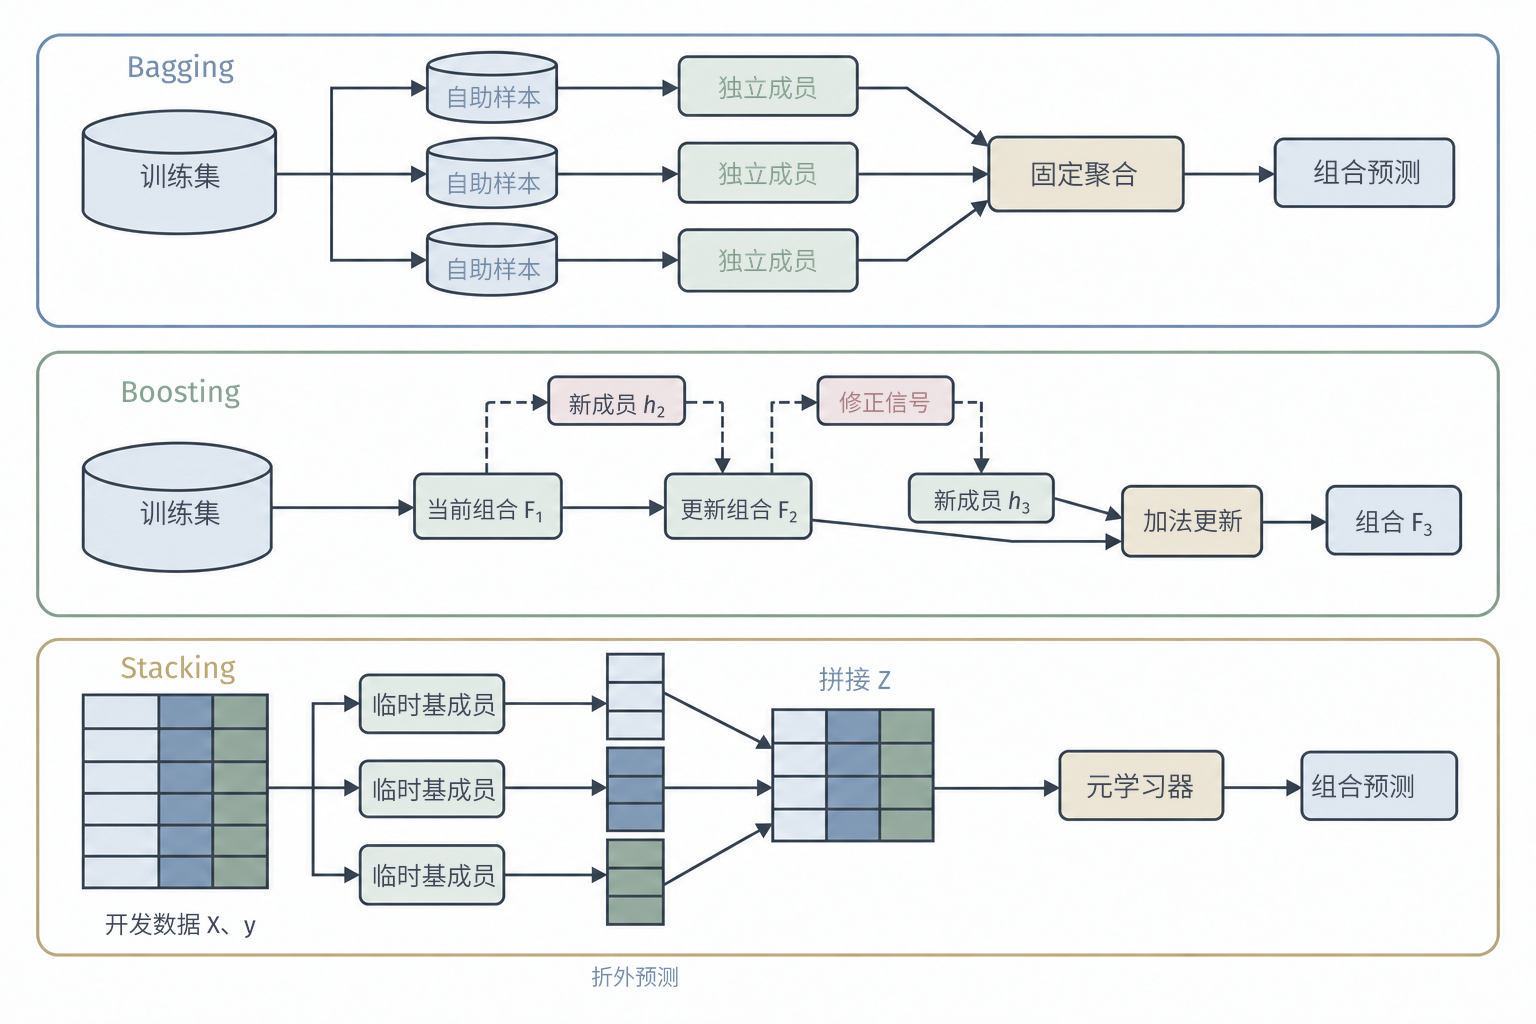
\includegraphics[width=130.048mm]{figures/03-models/01-classic-models/generated/ensemble-three-mechanisms/figure.png}
  \caption{Bagging、Boosting与Stacking的成员生成及组合关系。实线连接训练与预测步骤，虚线传递当前组合形成的修正信号。三类机制的成员依赖及组合规则不同；示意流程允许采用不同成员模型。}
  \label{fig:ensemble-three-mechanisms}
\end{figure*}

\paragraph{成员与组合输出}
\label{sec:ensemble-members-combination-output}

设训练集为
\[
  D_n=\{(\bm{x}_i,y_i)\}_{i=1}^{n},
\]
学习过程产生$M$个\term{成员模型}$h_1,\ldots,h_M$。用$\mathcal{C}$表示组合规则，\term{集成模型}的预测统一写成
\begin{equation}
  H(\bm{x})
  =\mathcal{C}\bigl(h_1(\bm{x}),\ldots,h_M(\bm{x})\bigr).
  \label{eq:ensemble-combination}
\end{equation}
式\eqref{eq:ensemble-combination}将成员预测映射为最终输出，具体规则由预测对象确定。回归成员若都预测同一个数值目标，可以采用等权平均
\[
  H(\bm{x})=\frac{1}{M}\sum_{m=1}^{M}h_m(\bm{x}),
\]
也可以用非负权重$w_m$作加权平均，其中$\sum_m w_m=1$。分类成员则可能输出硬标签、类别得分或类别概率。硬标签对应类别投票，同尺度得分或同类概率可逐类平均后决策；混合不同输出前，需要把它们转换为含义一致的量。

组合之前需要明确输出的数值含义。直接平均不同尺度的分类得分，会使数值范围较大的成员占据更大作用；平均类别概率则保持概率向量形式，其校准仍由新样本上的频率对应关系评价。元学习器若把得分转换为概率，这一映射也属于需要验证的模型。第\ref{sec:classification-evaluation}节分别给出了标签、排序与概率的评价方法。

权重的确定方式构成组合模型的一部分。等权平均固定每个成员的贡献，AdaBoost在序贯更新中估计贡献，线性Stacking根据折外预测学习权重。权重还可以依赖输入，此时$w_m=w_m(\bm{x})$，不同样本会调用不同成员或采用不同组合比例。成员数量、权重约束、组合层复杂度以及是否允许输入相关组合，都属于训练或验证流程需要确定的模型选择。


\section{基于Bagging的集成}
\label{sec:ensemble-bagging}

决策树的上层分裂可能随少量训练记录变化而改变，预测也随之波动。对同一总体的多份训练集分别建模并平均，可以削弱其中不共享的波动；实际通常只有一份数据，因而需要近似这种重复训练。\term{装袋法}（bootstrap aggregating, Bagging）用自助采样从现有训练集构造多份样本，分别训练成员，再用固定规则聚合。重采样使训练波动转为成员差异，固定聚合再削弱其中部分变化；成员共享的表示偏差则继续保留\scite{breiman1996bagging}。

\subsection{Bagging}
\label{sec:ensemble-bagging-bootstrap}

\subsubsection{自助样本与聚合预测}

对第$m$个成员，从$\{1,\ldots,n\}$中独立、等概率、有放回地抽取$n$次索引，所得多重集合记为$I^{(m)}$。有放回抽样使部分记录重复进入成员训练，也使部分记录留在该成员之外。学习算法$\mathcal{A}$在相应自助样本上训练出
\[
  h_m=\mathcal{A}\!\left(D_n^{(m)}\right),
  \qquad
  D_n^{(m)}=\{(\bm{x}_i,y_i):i\in I^{(m)}\}.
\]
回归通常平均$h_m(\bm{x})$；分类可以投票，也可以在成员输出具有同一语义时平均逐类得分或概率。可以改变自助样本大小或采用其他成员算法。此时仍需检验重采样是否使成员在新样本上产生互补预测。

一份大小为$n$的标准自助样本没有抽中原始样本$i$的概率为
\begin{equation}
  \mathbb{P}\!\left(i\notin I^{(m)}\right)
  =
  \left(1-\frac{1}{n}\right)^n
  \longrightarrow e^{-1}.
  \label{eq:ensemble-oob-probability}
\end{equation}
因此，每个成员平均约有$36.8\%$的原始样本未参与其训练。这些样本构成该成员的\term{袋外样本}（out-of-bag sample, OOB sample）。反过来，对每个训练样本$i$，可以只收集没有使用它训练的成员预测。令
\[
  \mathcal{M}_{i}^{\mathrm{OOB}}
  =\{m:i\notin I^{(m)}\},
\]
当$\mathcal{M}_{i}^{\mathrm{OOB}}$非空时，回归的袋外预测可写为
\begin{equation}
  \widehat{y}_{i}^{\mathrm{OOB}}
  =
  \frac{1}{|\mathcal{M}_{i}^{\mathrm{OOB}}|}
  \sum_{m\in\mathcal{M}_{i}^{\mathrm{OOB}}}h_m(\bm{x}_i),
  \label{eq:ensemble-oob-prediction}
\end{equation}
分类则对同一成员集合投票或平均类别输出。图\ref{fig:ensemble-bagging-oob}按样本收集符合条件的成员：每个样本的袋外预测由其未参与训练的成员子集给出，子集随样本变化。

\begin{figure*}[htbp]
  \centering
  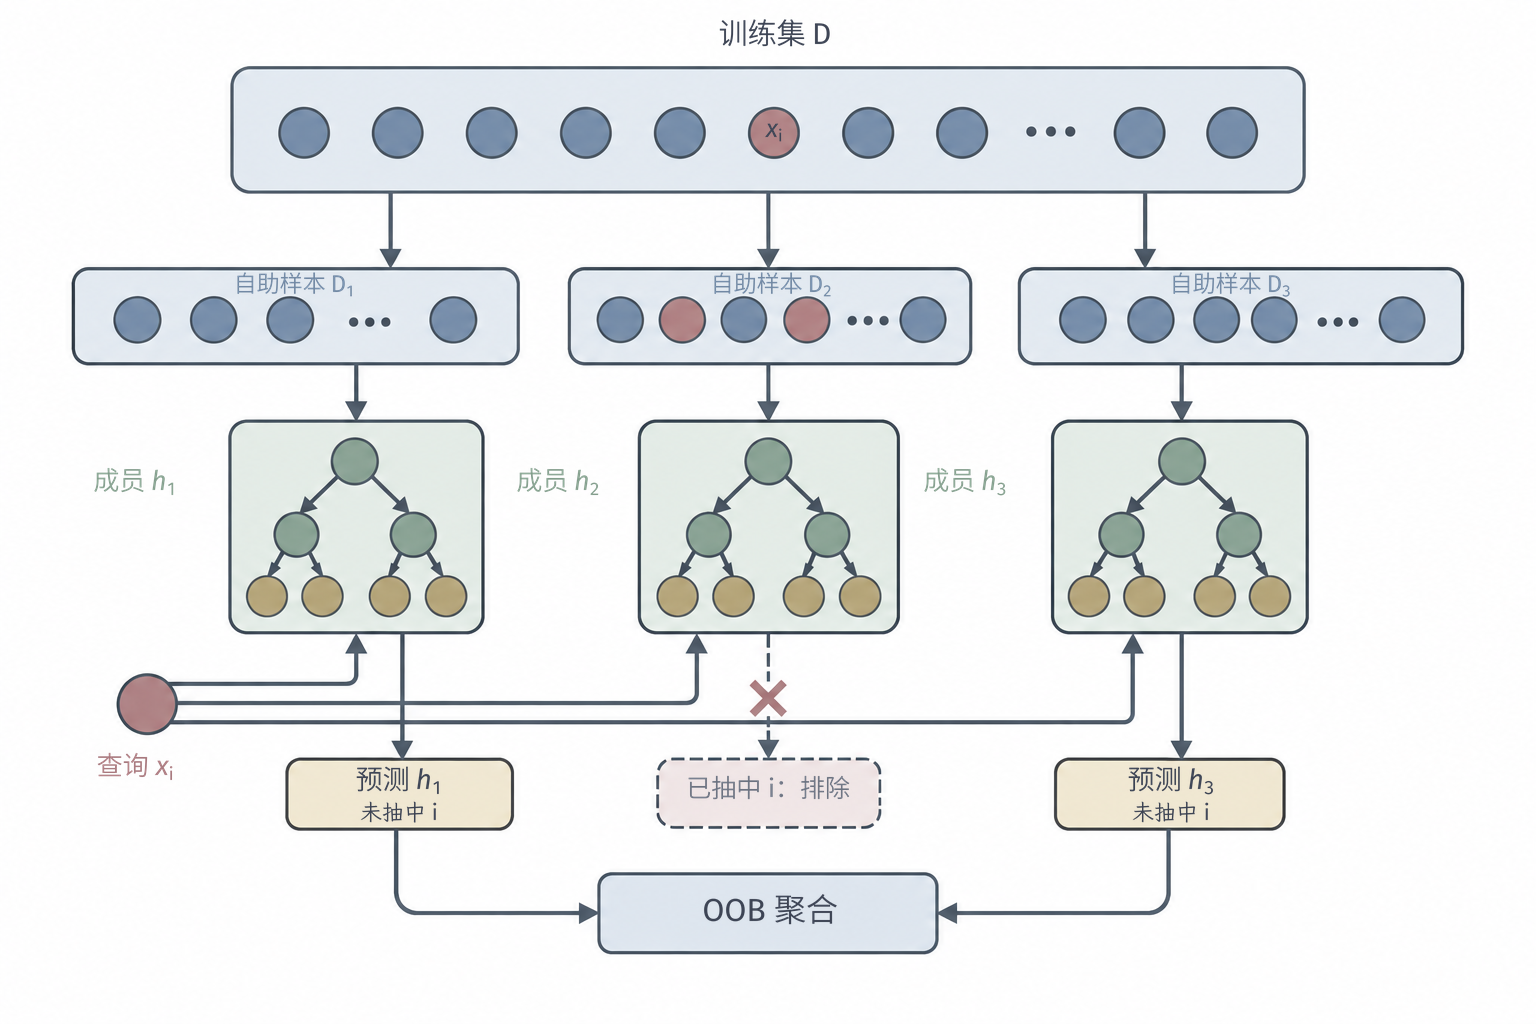
\includegraphics[width=130.048mm]{figures/03-models/01-classic-models/generated/ensemble-bagging-oob/figure.png}
  \caption{Bagging训练与袋外预测。每个成员只使用其自助样本训练；对训练样本$\bm{x}_i$，袋外预测只聚合未抽中$i$的成员。索引与集合展示样本和成员的对应关系；成员数有限时，各样本得到的袋外预测数量不同。}
  \label{fig:ensemble-bagging-oob}
\end{figure*}

\subsubsection{成员数量与误差来源}

给定原数据后，独立的重采样及训练可分配给不同计算单元。评价并行收益时，需要同时计入总工作量与实际经过时间：若单个成员的训练和预测成本分别为$C_{\mathrm{train}}$与$C_{\mathrm{pred}}$，朴素实现的总工作量仍约随$M C_{\mathrm{train}}$和$M C_{\mathrm{pred}}$增长。模型存储也通常随成员数量增加。

在固定训练集上增加独立随机成员，主要减少有限次抽样的Monte Carlo误差；等权平均逐渐逼近该随机训练机制的期望预测。原数据的抽样误差和模型失配仍影响这一期望，共同误差也会留在组合中。实践中可以观察袋外损失随成员数的变化，在曲线趋于稳定后停止增加成员，但这个停止规则也属于模型选择过程。

单树复杂度控制每份样本上的拟合，树数控制随机预测的平均程度。较深树可以表达更细的分区，也可能对扰动更敏感；叶规模与深度限制则可减少极小叶和噪声标签的影响。叶最小样本量、最大深度、类别权重和自助样本大小仍须与成员数共同选择，尤其在标签噪声、极小叶或类别极不平衡时。

\subsubsection{袋外预测的用途与边界}

袋外预测使当前标签与产生该预测的成员训练分离，可用于绘制树数—损失曲线、内部误差估计和置换重要性。可用成员数随机变化，自助训练集又相互重叠，这一数据结构与固定折的交叉验证不同。成员数很小时，某些样本可能没有足够的袋外预测。

反复用袋外结果选择结构、树数或特征处理，会使袋外误差成为开发证据；最终冻结流程需要另用测试数据评价。时间序列、分组样本或空间相关数据还要求自助抽样尊重依赖单位；逐行重采样会破坏原有数据结构。袋外结果的解释还依赖抽样单位与未来使用的数据制度。

\subsection{随机森林}
\label{sec:ensemble-random-forest}

树Bagging改变样本，却可能保留相同的强特征和上层分裂；这些共同选择使成员预测继续相关。\term{随机森林}（random forest）在树的自助采样之外加入节点级特征随机化：每个节点先随机抽取一组候选特征，再只在这组特征中搜索分裂。树仍按第\ref{sec:regression-trees}节或第\ref{sec:classification-trees}节的任务准则形成叶输出，改变的是每个成员可参与分裂搜索的信息\scite{breiman2001randomforests}。

节点候选特征数同时影响单树可用的信息和不同树的分裂差异。候选数接近全部特征时，森林更接近普通的树Bagging；候选数较小时，不同树更可能采用不同分裂，但单棵树也更容易错过当前节点上的有效特征。合适的候选规模取决于特征冗余、样本量和树深，可在固定验证协议下比较。

固定训练集并增加树数，可以减少森林平均预测的随机波动；所得极限仍由当前样本及树构造决定。总体风险另外受分布与估计条件控制，更多树也继续消耗存储和推理计算。随机森林的一致性结论通常针对特定的树构造、抽样比例与分布条件；实际软件在缺失值、类别特征、停止规则和并行实现上的差异，可能不满足同一组理论假设\scite{scornet2015consistency}。

\subsubsection{特征重要性的解释}

树集成常附带两类特征重要性。\term{不纯度下降重要性}（impurity-decrease importance）累计某个特征参与分裂时带来的加权目标下降，计算方便，却可能偏向候选切分较多的特征。相关变量可以在分裂中相互替代，累计下降反映实际选中的路径，因而与变量的独立贡献不同。

\term{置换重要性}（permutation importance）固定已训练模型，在评价数据上打乱一个特征，再观察预测损失增加多少。这个量直接对应已拟合模型在所选扰动下对该特征的依赖，但打乱会破坏该特征与其他特征的联合关系。高度相关的特征可能互相替代，使单个特征的置换影响看起来很小；不现实的特征组合也可能夸大损失变化。这些量分别描述训练分裂和预测扰动中的模型依赖，解释时需说明评价数据、损失及置换方式；因果判断另需因果假设与证据\scite{strobl2007bias}。

图\ref{fig:ensemble-tree-randomization}沿一棵树的构造路径比较三种随机化位置。树Bagging主要改变成员看到的训练样本；随机森林还在每个节点抽取候选特征；Extra Trees继续把随机性放入候选阈值。三者继续以任务准则比较分裂，差别在于进入贪心搜索的样本、特征和阈值。

\begin{figure*}[htbp]
  \centering
  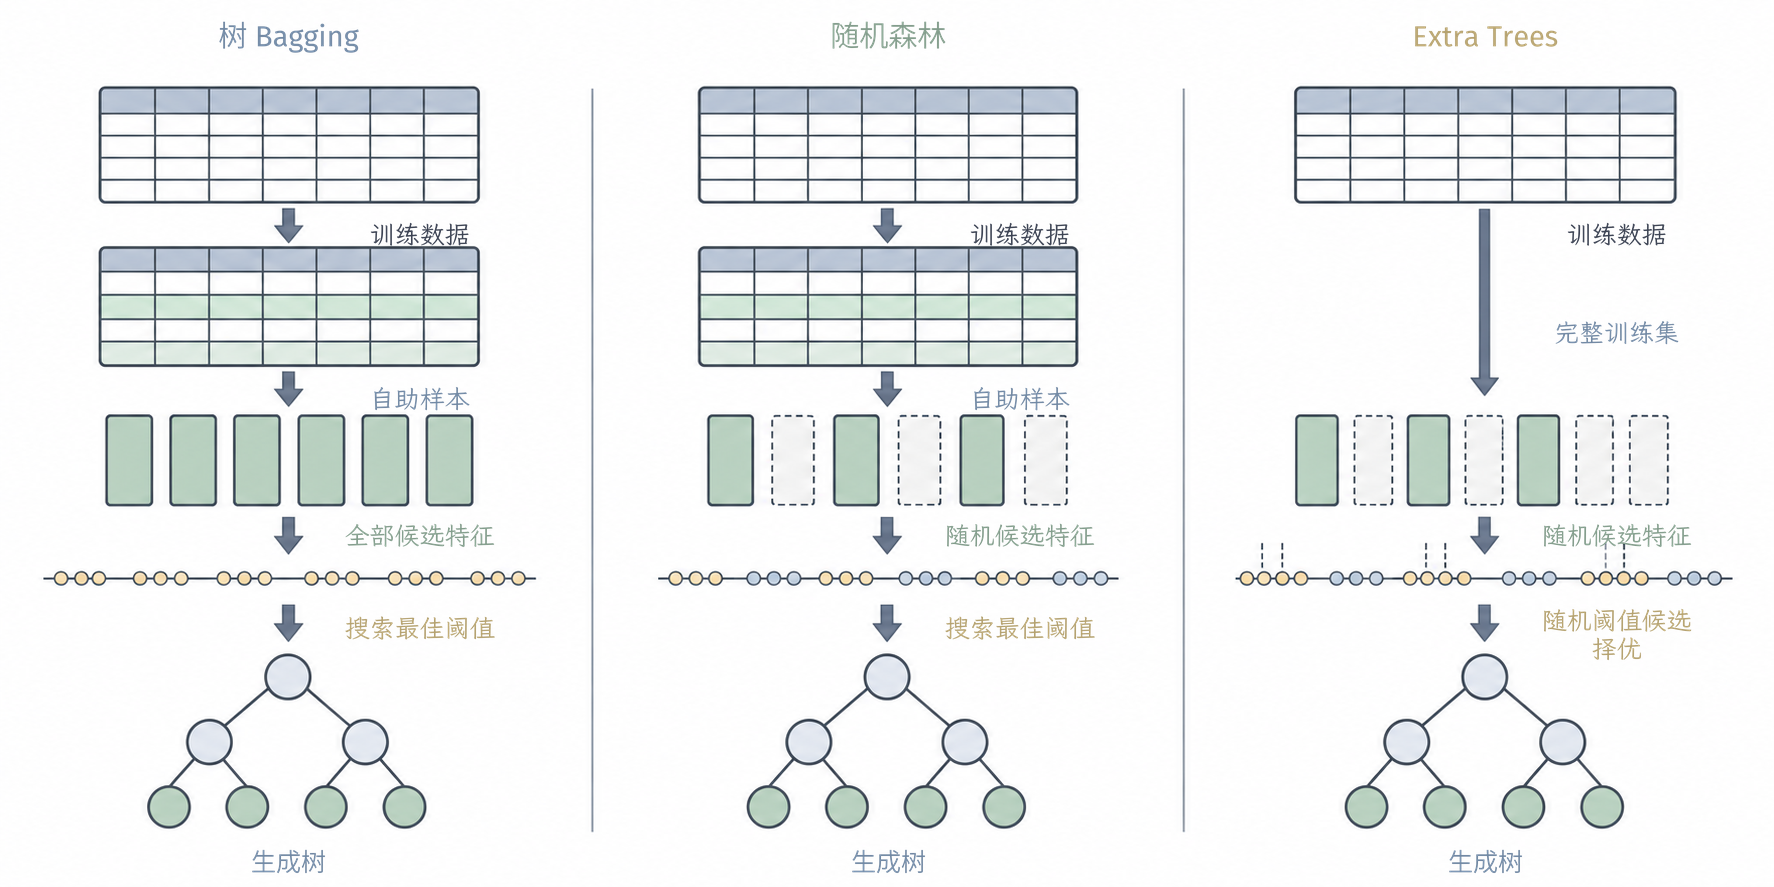
\includegraphics[width=150.199mm]{figures/03-models/01-classic-models/generated/ensemble-tree-randomization/figure.png}
  \caption{树Bagging、随机森林与Extra Trees的随机化位置。每栏从样本来源出发，依次展示候选特征、候选阈值与成员树；候选选择中的随机性和任务准则约束分别标在相应步骤。每栏首框直接标出训练样本来源：前两栏采用自助采样，Extra Trees栏采用原始方法的完整训练集设定；具体实现也可能额外启用自助采样。}
  \label{fig:ensemble-tree-randomization}
\end{figure*}

\subsection{极度随机树（Extra Trees）}
\label{sec:ensemble-extra-trees}

随机森林已随机选择候选特征，阈值仍通过当前节点的数据搜索。\term{极度随机树}（extremely randomized trees, Extra Trees）把随机性进一步放入阈值选择：在每个节点，对随机选出的候选特征生成随机切分点，再从这些随机候选中选择得分较好的切分。原始方法通常让各棵树使用完整训练集，把成员差异主要交给特征与阈值随机化；具体软件也可能允许额外使用自助采样\scite{geurts2006extra}。

随机阈值减少了穷举候选切分的工作，也会让单棵树偏离当前样本上的最佳贪心分裂。组合是否改善，取决于单树预测能力下降与成员依赖减弱之间的平衡。候选特征数、每个特征的随机阈值数、叶最小样本量以及是否采用自助采样共同决定这个平衡；增加随机化能否降低测试损失，需要在同一数据与预算下检验。

这些扩展可从“扰动发生在哪里”比较：在本节的宽泛机制分类中，样本、特征或阈值扰动都用于产生可独立训练的成员，再按固定规则聚合。标准Bagging则特指自助采样聚合。随机子空间只扰动成员可见的特征，Pasting以无放回子样本替代自助样本，随机权重则让同一记录在不同成员中具有不同影响。改变扰动方式后，袋外预测的可用条件也随是否采用自助采样而变化。

\subsection{模型对比与总结}
\label{sec:ensemble-bagging-comparison}

表\ref{tab:ensemble-bagging-comparison}固定树为成员，比较三种方法怎样产生差异。普通Bagging只改变训练样本；随机森林再限制节点可见的候选特征；Extra Trees进一步随机化候选阈值。三种方式还可能采用不同抽样方案，单树误差和搜索成本需与成员依赖一起比较。

\begin{table*}[htbp]
  \centering
  \small
  \begin{tabularx}{\linewidth}{@{}>{\raggedright\arraybackslash}p{24mm}*{6}{>{\raggedright\arraybackslash}X}@{}}
    \toprule
    方法 & 样本扰动 & 节点候选特征 & 阈值选择 & 袋外预测 & 成员训练 & 主要边界 \\
    \midrule
    树Bagging & 通常自助采样 & 全部特征 & 在候选中搜索 & 标准自助设定下可用 & 成员间可并行 & 强特征可能使树高度相关 \\
    随机森林 & 通常自助采样 & 随机特征子集 & 在子集内搜索 & 标准自助设定下可用 & 成员间可并行 & 候选数过小会削弱单树 \\
    Extra Trees & 原始方法使用完整训练集；实现可选自助采样 & 随机特征子集 & 生成随机阈值后择优 & 仅在采用自助采样时可用 & 成员间可并行 & 过强随机化会增大单树误差 \\
    \bottomrule
  \end{tabularx}
  \caption{以树为成员时，Bagging、随机森林与Extra Trees的机制比较。表中列出基本构造；比较具体实现时，还需记录抽样设置，并固定树复杂度、成员数和计算预算。}
  \label{tab:ensemble-bagging-comparison}
\end{table*}

Bagging先产生训练差异，再聚合预测以削弱部分波动。固定聚合保留成员共享的遗漏；若希望让新成员针对这些不足训练，就需要根据当前组合产生修正信号。下一节据此转向序贯提升。

\section{基于Boosting的集成}
\label{sec:ensemble-boosting}

Bagging分别训练成员后才聚合；如果希望新成员针对当前预测误差学习，就需要先计算已有组合的输出。\term{Boosting}（提升）构造一个序贯加法模型：第$t$轮先观察已有函数$F_{t-1}$，再选择新成员及其贡献，以降低指定训练目标。AdaBoost、梯度提升及现代提升树共享这种依赖关系，但它们生成修正信号和近似目标的方式不同。

\subsection{前向逐步加法模型}
\label{sec:ensemble-stagewise-additive}

设$F_0$为初始预测，Boosting经过$T$轮得到
\begin{equation}
  F_T(\bm{x})
  =
  F_0(\bm{x})
  +
  \sum_{t=1}^{T}\alpha_t h_t(\bm{x}),
  \label{eq:ensemble-additive-model}
\end{equation}
其中$h_t$是第$t$个成员，$\alpha_t$控制其贡献。为使复杂度惩罚对应真正加入模型的函数，把本轮增量记为$f_t=\alpha_t h_t$。给定损失$\ell$，理想化的第$t$轮直接优化增量：
\begin{equation}
  f_t
  \in
  \argmin_{f\in\mathcal{F}}
  \sum_{i=1}^{n}
  \ell\!\left(
    y_i,
    F_{t-1}(\bm{x}_i)+f(\bm{x}_i)
  \right)
  +\Omega_t(f).
  \label{eq:ensemble-forward-stagewise}
\end{equation}
这里$\mathcal{F}=\{\alpha h:\alpha\in\mathbb{R},h\in\mathcal{H}\}$是由成员函数族$\mathcal{H}$生成的增量函数族，$\Omega_t$是相应复杂度惩罚，也可以取零。

树的叶数惩罚控制分区规模，叶输出范数惩罚控制本轮增量。范数应作用于$f$，使惩罚随实际加入组合的幅度变化；若仅惩罚$h$，它与$\alpha$的相互缩放会改变惩罚却保持预测。

逐步优化固定已有成员，减少了联合搜索变量，但最优范围仅限本轮增量。后文用梯度拟合、二阶目标和收缩构造近似更新。

不同方法将当前预测转换为不同的训练信号。AdaBoost改变训练样本的权重，使当前错分记录在下一轮具有更大影响；梯度提升把损失对当前预测的负梯度作为伪响应；二阶提升树还利用局部曲率近似叶权重和分裂收益。平方损失的负梯度恰为普通响应残差，其他损失则给出不同修正量。损失决定了下一轮成员拟合的对象。

\subsection{AdaBoost}
\label{sec:ensemble-adaboost}

\term{AdaBoost}（adaptive boosting）通过更新样本权重，使新分类器更多地处理当前组合反复错分的记录。考虑二分类标签$y_i\in\{-1,1\}$和成员$h_t(\bm{x})\in\{-1,1\}$。初始样本权重为$w_i^{(1)}=1/n$，第$t$轮成员的加权错误率为
\begin{equation}
  \epsilon_t
  =
  \sum_{i=1}^{n}
  w_i^{(t)}
  \mathbb{I}\!\left\{y_i\neq h_t(\bm{x}_i)\right\}.
  \label{eq:ensemble-adaboost-error}
\end{equation}
当$0<\epsilon_t<1/2$时，成员投票权重取
\begin{equation}
  \alpha_t
  =
  \frac{1}{2}
  \log\frac{1-\epsilon_t}{\epsilon_t},
  \qquad
  w_i^{(t+1)}
  =
  \frac{
    w_i^{(t)}
    \exp\!\left[-\alpha_t y_i h_t(\bm{x}_i)\right]
  }{Z_t},
  \label{eq:ensemble-adaboost-update}
\end{equation}
其中$Z_t$使新权重和为1。错分样本满足$y_i h_t(\bm{x}_i)=-1$，权重乘上$e^{\alpha_t}$；正确样本的权重乘上$e^{-\alpha_t}$。

若$\epsilon_t=0$，在这些正权重下当前成员已分对全部训练样本，便直接输出$h_t$并停止，避免将发散系数代入更新（参考\BookSectionRef{sec:boosting}{第二卷“基础、理论和可信性”的“二分类学习的可学习性”章“集成学习”节}）。其余情况下，最终分类器在预先固定平局规则后按$\operatorname{sign}(\sum_t\alpha_t h_t(\bm{x}))$决策。正的成员贡献要求当前加权错误率小于$1/2$；条件未满足时，可停止本轮、调整训练或采用相应变体。

图\ref{fig:ensemble-adaboost-weight-update}将分类错误与下一轮权重连接起来。当前分类结果先改变样本权重，再由归一化后的权重决定下一轮成员看到的训练分布；错分记录因而获得更大的后续影响。

\begin{figure*}[htbp]
  \centering
  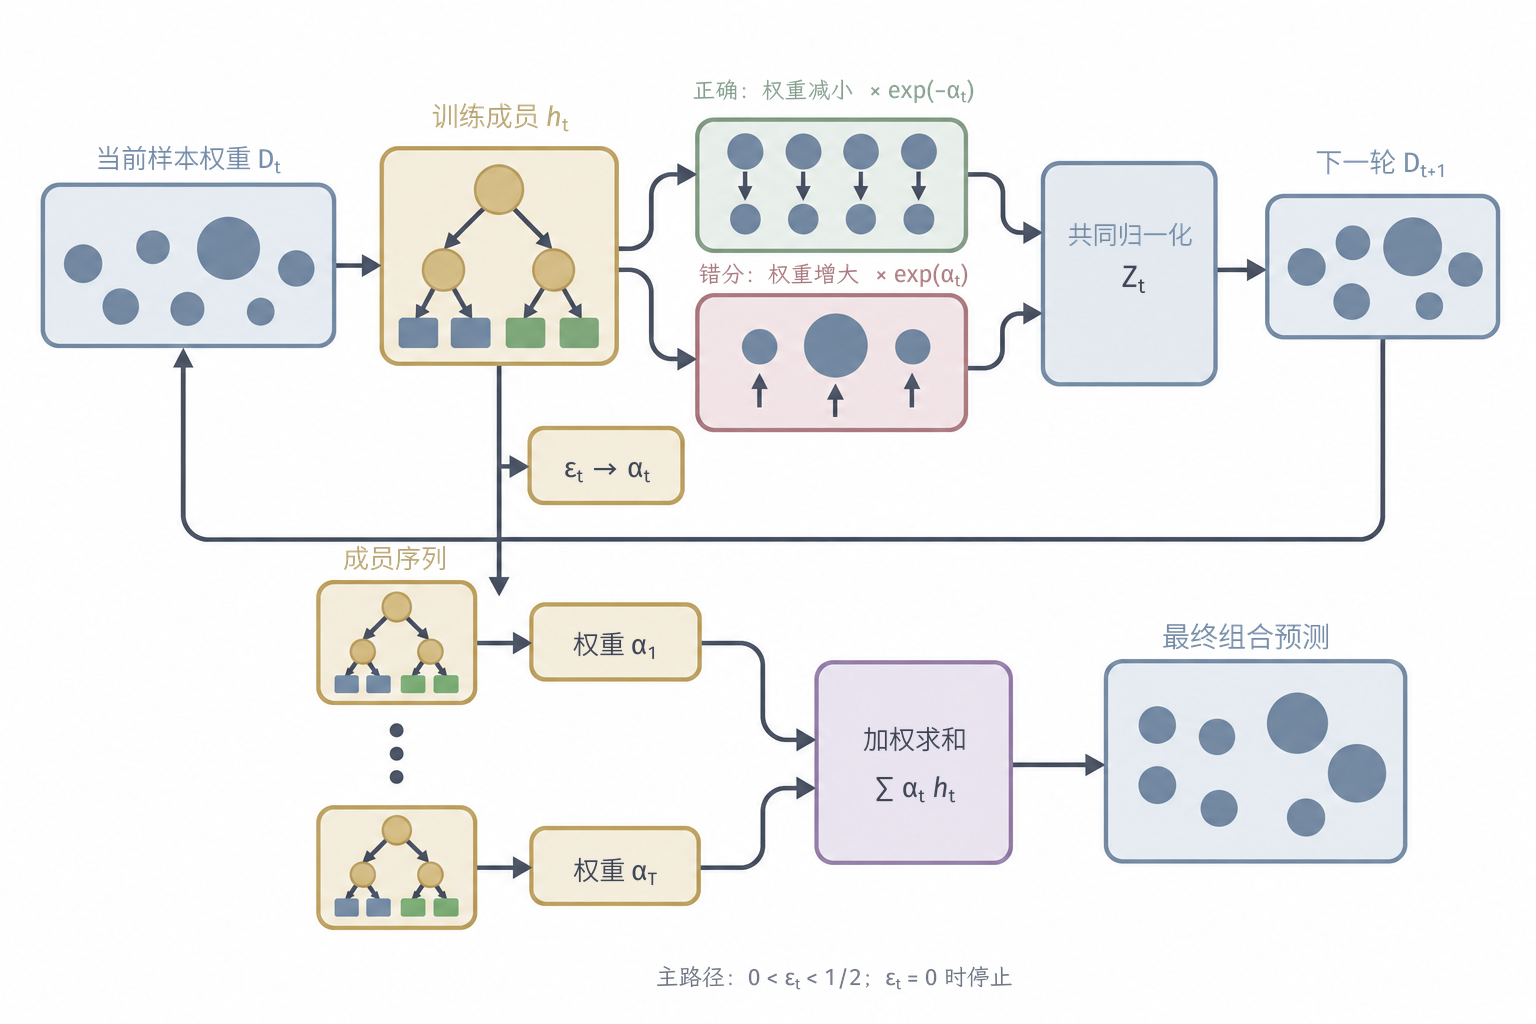
\includegraphics[width=130.048mm]{figures/03-models/01-classic-models/generated/ensemble-adaboost-weight-update/figure.png}
  \caption{AdaBoost的样本权重更新。分类结果把样本分成正确与错分两路，两路缩放后的权重汇合并归一化，形成下一轮训练分布。实线连接各更新步骤；绿色框标示正确分类样本的减权，红色框标示错分样本的增权。}
  \label{fig:ensemble-adaboost-weight-update}
\end{figure*}

这一更新也可以从指数损失解释。令$F(\bm{x})=\sum_t\alpha_t h_t(\bm{x})$，经验目标为
\[
  \sum_{i=1}^{n}\exp\!\left[-y_iF(\bm{x}_i)\right].
\]
固定$F_{t-1}$后选择$h_t$与$\alpha_t$，在$0<\epsilon_t<1/2$时可以导出式\eqref{eq:ensemble-adaboost-update}。样本重加权由指数损失的逐步优化导出，因此其作用可以通过该目标分析\scite{freund1997boosting,friedman2000adaboost}。

持续错分的记录获得更大权重，后续成员因而可能恢复稀少的边界结构，也可能追逐错误标签。若每轮的带权错误率均在$(0,1/2)$内，指数损失分析给出训练误差上界；各轮优势若有统一的正下界，这个上界随轮数指数下降。新样本风险则还要控制归一化投票间隔和预先固定的基函数类复杂度（参考\BookSectionRef{sec:boosting}{第二卷“基础、理论和可信性”的“二分类学习的可学习性”章“集成学习”节}）。实际训练需同时检查错误记录的来源、训练目标和独立测试表现。

多分类AdaBoost需要重新定义成员错误与类别得分，回归变体则要用响应误差决定样本权重和预测聚合。这些变体沿用序贯重加权，但成员错误、系数与聚合需要按各自任务重新推导。评价分别采用分类或回归的输出和损失。

\subsection{梯度提升机与GBDT}
\label{sec:ensemble-gradient-boosting}

改变任务损失后，也需要改变修正信号。对于关于预测可微的损失，其负梯度指出当前预测降低经验目标的方向。\term{梯度提升机}（gradient boosting machine, GBM）用基学习器逼近这个负梯度方向，从而把序贯加法扩展到更一般的损失\scite{friedman2001gradientboost}。

通常从使训练损失最小的常数预测开始：
\begin{equation}
  F_0(\bm{x})=c_0,
  \qquad
  c_0\in\argmin_c\sum_{i=1}^{n}\ell(y_i,c).
  \label{eq:ensemble-gbm-initialization}
\end{equation}
平方损失下$c_0$是响应均值。这里要求存在有限的最小化点；若某种损失与数据组合使最优常数趋于无穷，就需约束预测范围或另定有限初始化。

在第$t$轮，对每个训练样本计算\term{伪残差}（pseudo-residual），即损失在当前预测处的负导数：
\begin{equation}
  r_i^{(t)}
  =
  -
  \left.
  \frac{\partial \ell(y_i,z)}{\partial z}
  \right|_{z=F_{t-1}(\bm{x}_i)}.
  \label{eq:ensemble-pseudo-residual}
\end{equation}
随后用平方误差把这些修正量拟合到成员函数族：
\begin{equation}
  h_t\in\argmin_{h\in\mathcal{H}}
  \sum_{i=1}^{n}\bigl(r_i^{(t)}-h(\bm{x}_i)\bigr)^2.
  \label{eq:ensemble-gbm-gradient-fit}
\end{equation}
此处平方误差衡量成员对负梯度的逼近，即使原任务采用其他损失也使用这一拟合对象。贪心树生长通常给出子问题的近似解。

固定$h_t$后，可以按原损失做整体线搜索，在最小值存在时取
\begin{equation}
  \alpha_t\in\argmin_\alpha
  \sum_{i=1}^{n}
  \ell\!\left(y_i,F_{t-1}(\bm{x}_i)+\alpha h_t(\bm{x}_i)\right).
  \label{eq:ensemble-gbm-line-search}
\end{equation}
此处$\alpha_t$是整棵树或整个成员共享的一个标量。加入预先选择的收缩系数$\eta\in(0,1]$后，
\begin{equation}
  F_t(\bm{x})
  =
  F_{t-1}(\bm{x})
  +
  \eta\alpha_t h_t(\bm{x}).
  \label{eq:ensemble-gradient-boosting-update}
\end{equation}


当$\ell(y,z)=\tfrac12(y-z)^2$时，式\eqref{eq:ensemble-pseudo-residual}给出$y_i-F_{t-1}(\bm{x}_i)$，恰好是普通残差。分类时则要先明确得分与概率的关系。例如二分类采用$y_i\in\{0,1\}$，令$F$表示对数几率（logit），相应概率与二项对数损失为
\[
  p=\sigma(F)=\frac{1}{1+e^{-F}},\qquad
  \ell(y,F)=\log(1+e^F)-yF.
\]
由于$\partial\ell/\partial F=\sigma(F)-y$，第$t$轮的伪残差为
\[
  r_i^{(t)}=y_i-p_i^{(t-1)},\qquad
  p_i^{(t-1)}=\sigma\!\left(F_{t-1}(\bm{x}_i)\right).
\]


例如$y_i=1$而当前概率为$0.3$时，伪残差为$0.7$，表示损失对得分的修正信号。成员拟合后将增量加到$F$，再经Sigmoid换算概率；修正量与概率因此处于不同数值空间。

若$h_t$采用回归树，就得到\term{梯度提升决策树}（gradient boosting decision tree, GBDT）。除了整体线搜索，还可以保留平方拟合得到的叶区域$\bm{R}_1^{(t)},\ldots,\bm{R}_{L_t}^{(t)}$，再按原损失分别求每片叶的增量。当各叶内存在有限最小化点时，
\begin{equation}
  \begin{aligned}
    v_j^{(t)}
      &\in\argmin_v
        \sum_{i:\,\bm{x}_i\in\bm{R}_j^{(t)}}
        \ell\!\left(y_i,F_{t-1}(\bm{x}_i)+v\right),\\
    F_t(\bm{x})
      &=F_{t-1}(\bm{x})
        +\eta\sum_{j=1}^{L_t}
        v_j^{(t)}\mathbb{I}\{\bm{x}\in\bm{R}_j^{(t)}\}.
  \end{aligned}
  \label{eq:ensemble-gbm-leaf-update}
\end{equation}
$L_t$表示叶数，各叶分别选择$v_j^{(t)}$并替换原树输出；这与整棵树共用一个$\alpha_t$是两种更新方案。有限叶内最小值不存在时，需要限制输出或增加正则后再更新。回归树在这里承担连续修正量的拟合，最终任务也可以是分类。

第\ref{sec:regression-quantiles}节的分位数损失$\ell(y,z)=\rho_\tau(y-z)$在$z=y$处不可微，修正信号需改为次梯度。分位数提升可改用负次梯度，例如约定
\begin{equation}
  r_i^{(t)}
  =\tau-\mathbb{I}\{y_i<F_{t-1}(\bm{x}_i)\},
  \qquad 0<\tau<1.
  \label{eq:ensemble-quantile-pseudo-residual}
\end{equation}
等号处的负次梯度可取$[\tau-1,\tau]$内任意值，这里选端点$\tau$。常数初始化取样本$\tau$分位数，仍用平方误差拟合上述修正量；逐叶更新则最小化原分位数损失，故$v_j^{(t)}$取该叶内普通残差$y_i-F_{t-1}(\bm{x}_i)$的$\tau$分位数，而不是伪残差的均值。

学习率、轮数与单树复杂度共同决定加法函数。较小学习率缩小每轮变化，通常需要更多轮才能达到相近训练目标；较深的树可以在单轮表达更高阶交互，也会扩大每轮容量。行采样和列采样进一步引入随机性，早停则依据独立验证轨迹选择轮数。选择学习率时需同时调整轮数，并在给定树复杂度、采样和早停协议下比较。

下一轮使用当前组合的梯度，GBM各轮因而按序执行。单轮内部仍可并行统计不同特征或候选分裂。训练损失描述经验拟合，停止轨迹描述求解，测试风险描述未来预测；若轮数、损失、树结构和早停规则都根据同一验证集反复调整，还要把这种选择纳入最终评价。

\subsection{XGBoost}
\label{sec:ensemble-xgboost}

经典梯度提升用一阶负梯度给出拟合方向。\term{XGBoost}在正则化加法树目标中进一步使用二阶局部近似，并围绕稀疏输入、近似分裂和内存访问设计训练系统\scite{chen2016xgboost}。二阶目标给出候选树的评分，分裂算法搜索结构，系统设计组织统计量的计算与访问。三层共同形成实现，但回答不同问题。

设第$t$棵树为$f_t$，损失在当前预测$F_{t-1}(\bm{x}_i)$处的一阶导与二阶导分别为$g_i^{(t)}$和$s_i^{(t)}$。去掉与$f_t$无关的常数后，本轮目标近似为
\begin{equation}
  \widetilde{\mathcal{L}}^{(t)}
  =
  \sum_{i=1}^{n}
  \left[
    g_i^{(t)}f_t(\bm{x}_i)
    +\frac{1}{2}s_i^{(t)}f_t^2(\bm{x}_i)
  \right]
  +\gamma L
  +\frac{\lambda}{2}\sum_{j=1}^{L}v_j^2,
  \label{eq:ensemble-xgboost-objective}
\end{equation}
其中$L$是叶数，$v_j$是第$j$片叶的输出，$\gamma$惩罚新增叶，$\lambda$约束叶权重。若$I_j$表示落入第$j$片叶的样本索引，记
\[
  G_j=\sum_{i\in I_j}g_i^{(t)},
  \qquad
  S_j=\sum_{i\in I_j}s_i^{(t)}.
\]
在$S_j+\lambda>0$时，固定树结构的最优叶权重为
\begin{equation}
  v_j^\star=-\frac{G_j}{S_j+\lambda}.
  \label{eq:ensemble-xgboost-leaf-weight}
\end{equation}
把一个父叶分成左右子叶时，相应近似目标下降量为
\begin{equation}
  \operatorname{Gain}
  =
  \frac{1}{2}
  \left[
    \frac{G_{\mathrm{L}}^2}{S_{\mathrm{L}}+\lambda}
    +
    \frac{G_{\mathrm{R}}^2}{S_{\mathrm{R}}+\lambda}
    -
    \frac{(G_{\mathrm{L}}+G_{\mathrm{R}})^2}
         {S_{\mathrm{L}}+S_{\mathrm{R}}+\lambda}
  \right]
  -\gamma.
  \label{eq:ensemble-xgboost-split-gain}
\end{equation}
式\eqref{eq:ensemble-xgboost-split-gain}把当前损失的梯度、曲率与树复杂度放在同一个分裂准则中。增益评价局部二阶目标在当前分裂下的变化；贪心生长只搜索逐步形成的结构。

图\ref{fig:ensemble-gradient-xgboost}把一阶梯度提升与XGBoost的二阶树评分放在同一计算链中。左图用负梯度定义拟合对象，右图从候选区域的梯度统计计算叶权重和分裂增益；二阶统计扩展了本轮目标的近似信息，但没有改变逐轮加法更新的外层结构。

\begin{figure*}[htbp]
  \centering
  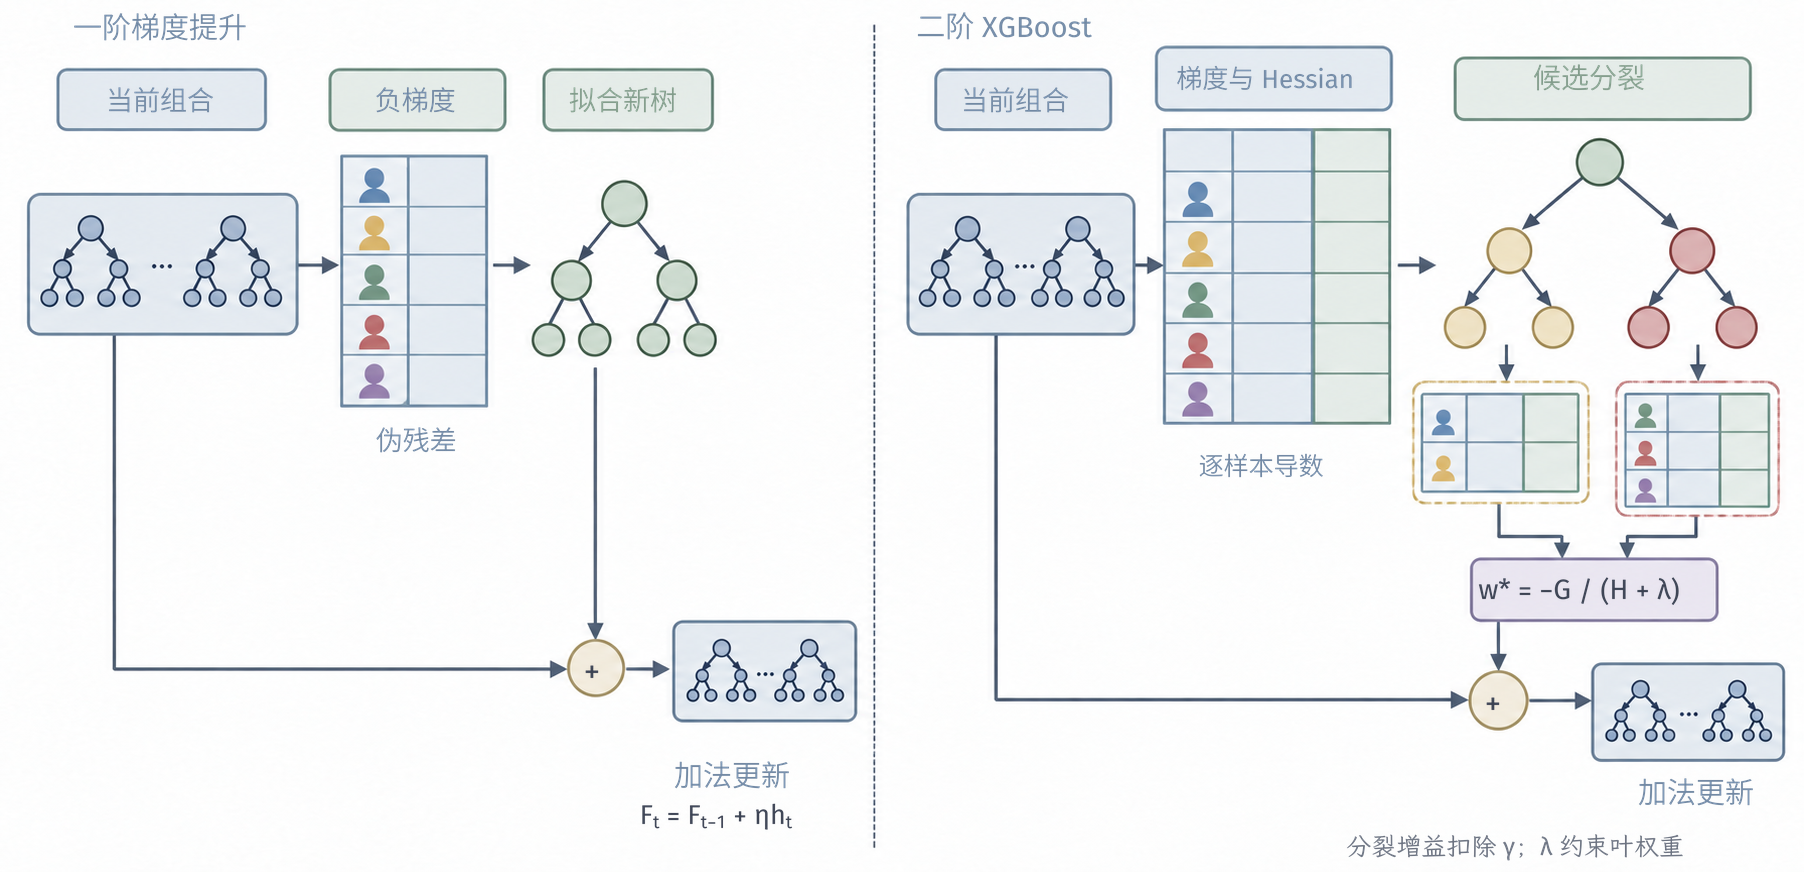
\includegraphics[width=152.739mm]{figures/03-models/01-classic-models/generated/ensemble-gradient-xgboost/figure.png}
  \caption{梯度提升与XGBoost中的本轮修正。左图中，损失对当前预测的负梯度形成伪残差，新成员拟合该信号后更新组合；右图中，XGBoost按候选分裂聚合一阶导与二阶导，再由同一组叶统计计算叶权重和分裂增益。图中单叶权重$w^\ast$对应正文的$v_j^\star$，$G$与$H$分别表示叶内一阶导和二阶导之和。复杂度项$\gamma T+\lambda\lVert\bm{w}\rVert_2^2/2$中的$T$为叶数，$\bm{w}$汇集各叶输出；$\lambda$限制叶权重，$\gamma$惩罚新增叶。该图展示当前候选树的局部评分。}
  \label{fig:ensemble-gradient-xgboost}
\end{figure*}

精确分裂搜索遍历排序后的候选特征值；近似搜索则先用带权分位数草图构造候选切分，再汇总梯度统计。稀疏感知搜索为缺失值学习默认方向，列采样减少每轮需要检查的特征。块式存储、缓存感知访问、并行统计和外存计算改变的是实现代价，不改变式\eqref{eq:ensemble-xgboost-objective}所定义的学习对象。这些设计在特定硬件和数据规模上的时间收益可通过完整训练测量确认。

\subsection{LightGBM}
\label{sec:ensemble-lightgbm}

逐值分裂搜索需要遍历候选取值，样本和特征增多会扩大这一工作量。\term{LightGBM}以直方图训练为基础，把连续特征映射到有限个桶，并在桶级别累计梯度和曲率。构造直方图仍要访问节点样本，但候选分裂只需扫描桶；已知父节点和一个子节点的直方图时，还可以用差分得到另一个子节点的统计量。分桶减少存储和候选数，也引入离散化误差。

树的生长顺序进一步改变计算分配。按层生长同时扩展某一深度上的叶，按叶生长则每次选择当前增益最大的叶继续分裂。在相同叶数下，后者把容量集中到训练目标下降较大的局部区域，可能形成深度不均衡的树。叶数、最小叶样本量和深度共同限制这种局部扩展，训练收益再由验证或测试检查其样本外效果。

LightGBM论文进一步提出两种针对大规模数据的近似。\term{单边梯度采样}（gradient-based one-side sampling, GOSS）保留绝对梯度较大的样本，从绝对梯度较小的样本中随机抽取一部分，并在分裂统计中重新加权后者。例如，在小梯度组内等概率抽取一半样本，就把被抽中者对梯度和的贡献乘二，以补偿未采样部分。一般地，样本以概率$p>0$被保留时，其贡献乘以$1/p$；给定本轮梯度和候选分区，这种逆包含概率加权可无偏估计相应的梯度和，平方、比值及择优得到的增益则是非线性量，其偏差需另行分析。

\term{互斥特征捆绑}（exclusive feature bundling, EFB）把很少同时非零的稀疏特征编码到较少的组合特征中，近似减少有效特征数。GOSS、EFB和直方图分别减少样本统计、特征表示和阈值候选，可按各自近似对象评价误差与计算节省\scite{ke2017lightgbm}。

图\ref{fig:ensemble-lightgbm-approximations}按近似对象并列这三种机制。直方图压缩候选阈值，GOSS压缩参与分裂统计的样本，EFB压缩稀疏特征表示；这三个对象分别对应数据访问、有效特征数与候选扫描的成本。

% Flush preceding margin references before the full-width illustration.
\clearpage
\begin{figure*}[htbp]
  \centering
  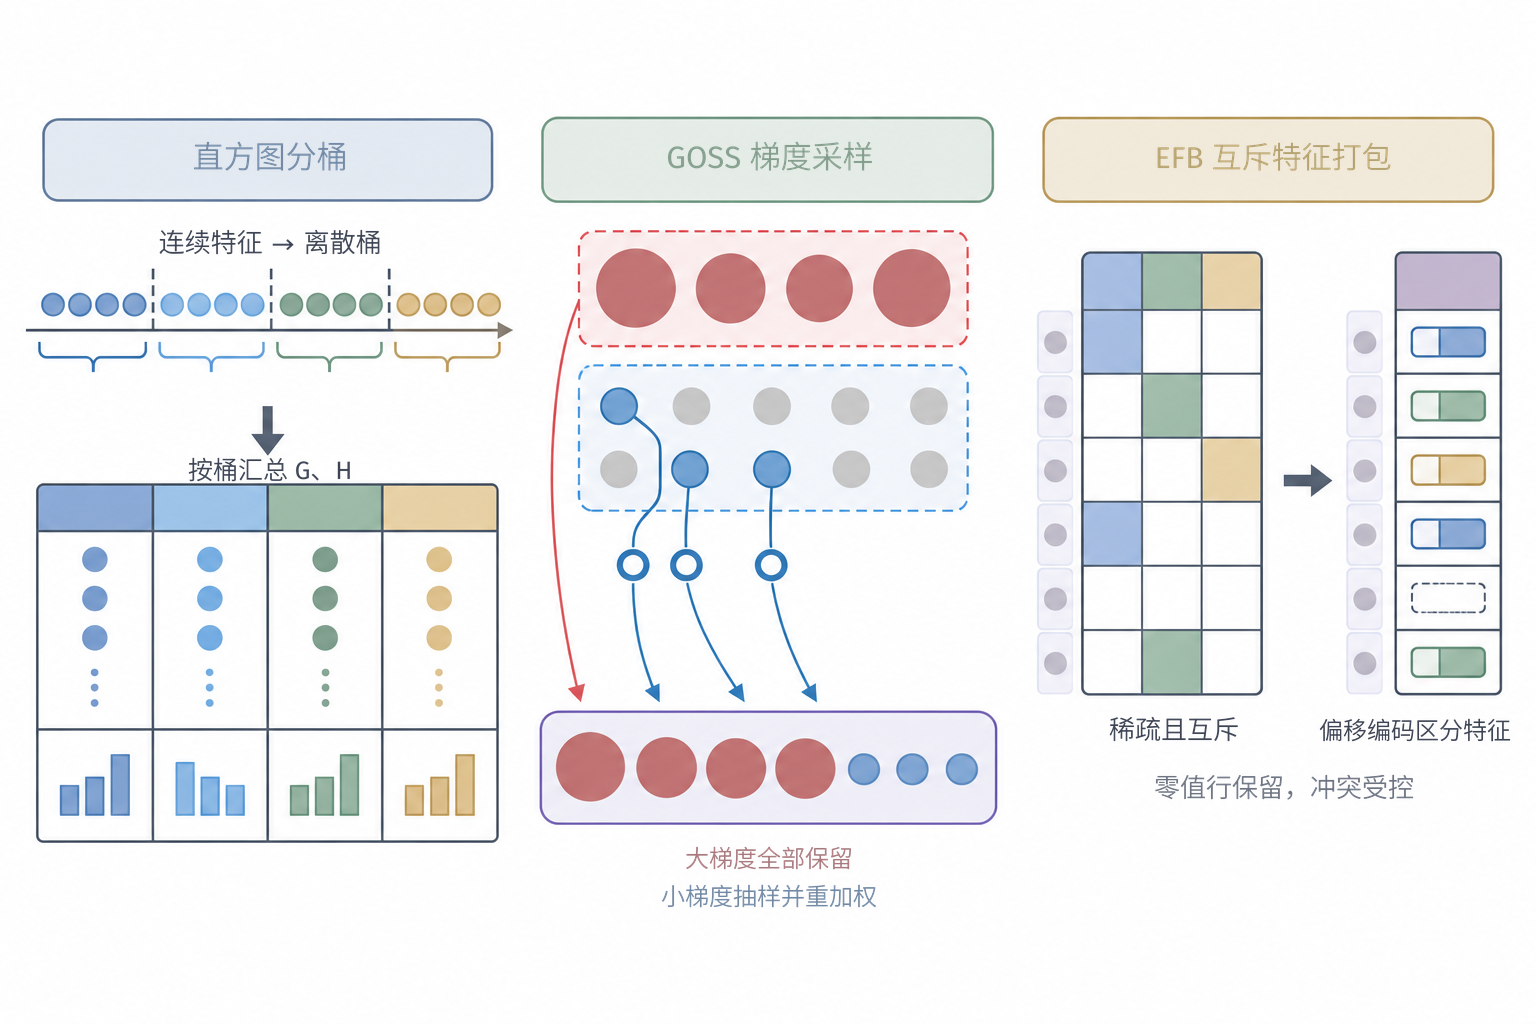
\includegraphics[width=130.048mm]{figures/03-models/01-classic-models/generated/ensemble-lightgbm-approximations/figure.png}
  \caption{LightGBM中三种作用位置不同的计算近似。直方图把连续取值映射到有限桶，GOSS保留$|g_i|$较大的样本，并抽取、重加权部分$|g_i|$较小的样本，EFB把很少同时非零的特征编码为较少的捆绑特征。图中点数、桶数与非零位置均为机制示意。}
  \label{fig:ensemble-lightgbm-approximations}
\end{figure*}

这些机制的效果依赖梯度分布、特征稀疏性、桶数、冲突处理和硬件实现。比较速度和任务损失时，需要记录数据规模、硬件、桶数与采样设置，并固定搜索预算及早停规则。论文实验的结论据此限定于相应条件。

\subsection{CatBoost}
\label{sec:ensemble-catboost}

高基数类别特征若全部展开为独热变量，会增加特征规模；把类别直接映射为整数，又会引入原本不存在的次序。另一种做法是用同类别样本的响应均值编码，但若样本自己的$y_i$参与其编码，模型就能从输入中间接看到待预测标签。训练输入含有待预测响应、部署输入却没有，这种构造差异称为\term{目标泄漏}（target leakage）。

\term{CatBoost}用随机排列建立\term{有序目标统计}（ordered target statistic）。设$c_i$为样本$i$的某个类别值，用$\pi(j)$表示样本$j$在随机排列中的位置；对当前样本只使用排列中位于它之前且类别相同的记录：
\begin{equation}
  z_i
  =
  \frac{
    \sum_{j:\,\pi(j)<\pi(i)}
    \mathbb{I}\{c_j=c_i\}y_j
    +ap
  }{
    \sum_{j:\,\pi(j)<\pi(i)}
    \mathbb{I}\{c_j=c_i\}
    +a
  }.
  \label{eq:ensemble-catboost-ordered-statistic}
\end{equation}
其中$p$是先验统计量，$a>0$控制平滑。前缀统计排除了样本自身的标签，部署时可从已观测的训练记录形成同类别统计。低频类别仍会产生较大估计波动，平滑、多个排列和类别组合需要共同考虑。

图\ref{fig:ensemble-catboost-ordered-statistics}固定当前样本的排列位置，检查哪些标签进入编码。计算当前类别$A$样本的编码时，只允许排列前缀中同为类别$A$的标签进入统计量；其他类别、当前标签和排列后缀都不参与这次编码。

\begin{figure*}[htbp]
  \centering
  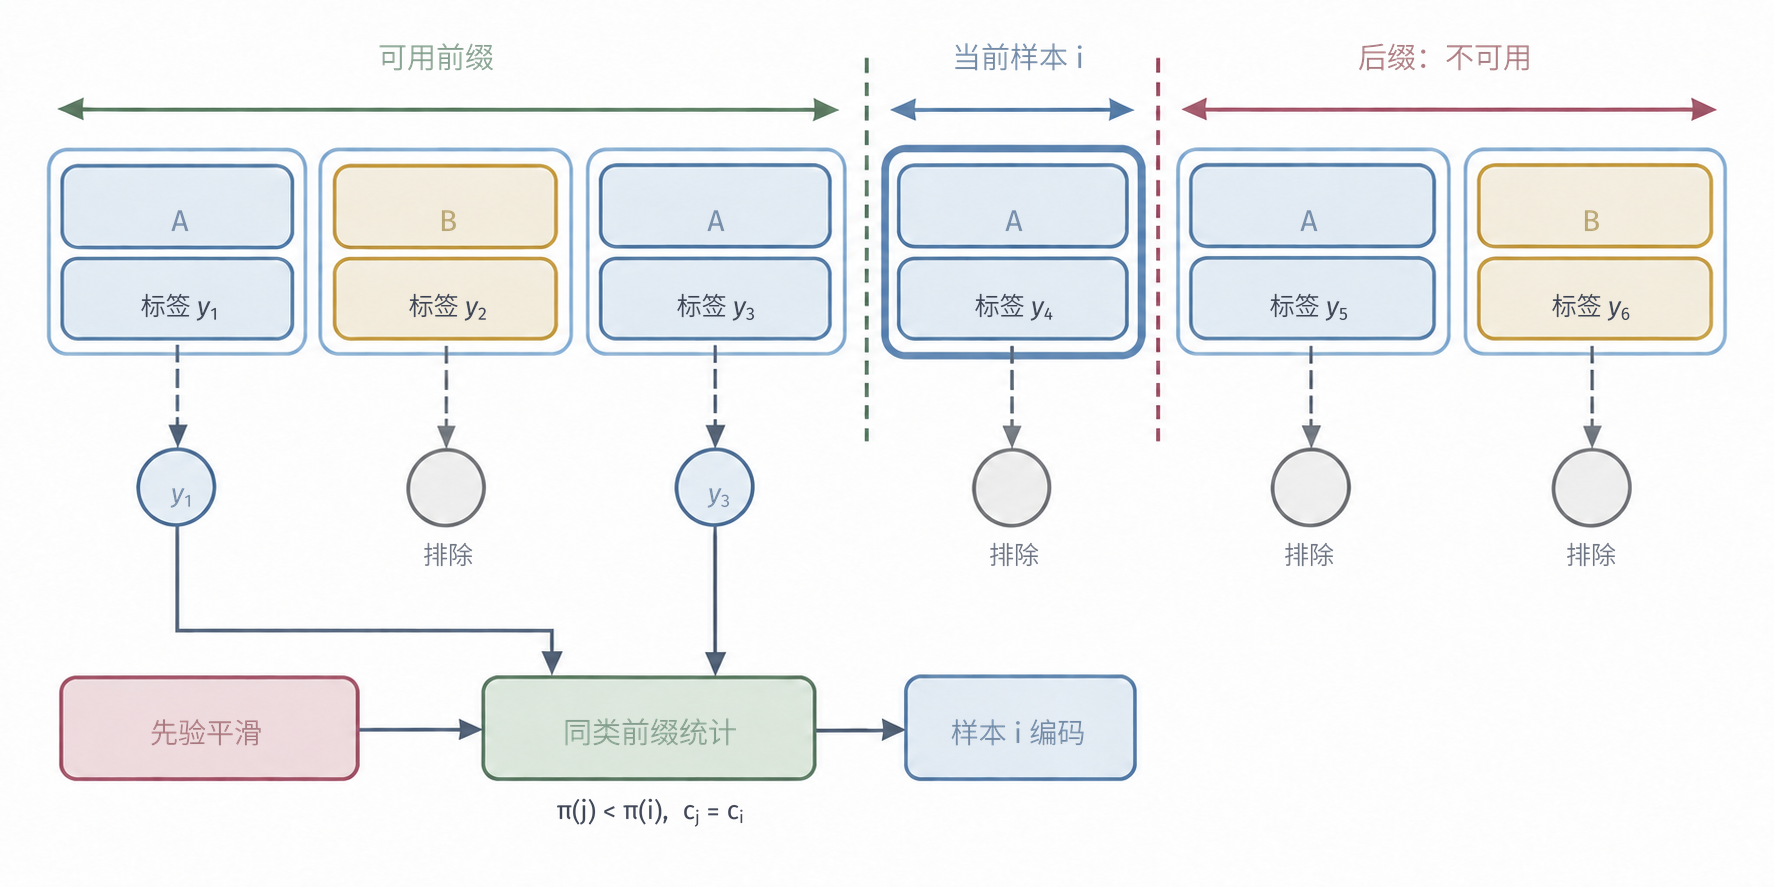
\includegraphics[width=150.199mm]{figures/03-models/01-classic-models/generated/ensemble-catboost-ordered-statistics/figure.png}
  \caption{CatBoost有序目标统计的前缀约束。这里$\pi(j)$表示样本$j$在随机排列中的位置；计算当前样本$i$的编码时，只有满足$\pi(j)<\pi(i)$且$c_j=c_i$的标签通过实线汇入统计量。其他类别、当前标签和后续记录均不连接到统计量，表示它们在本次编码中被隔离。样本索引与类别符号仅用于说明机制。}
  \label{fig:ensemble-catboost-ordered-statistics}
\end{figure*}

有序提升把相同的前缀思想用于梯度估计。计算当前样本的预测与梯度时，采用由其前缀记录拟合的相应模型，使该样本的标签与当前预测拟合分离，以减少这一重复使用带来的预测偏移。实际算法通过多个排列和前缀模型实现这一约束，训练状态与计算量也比普通单序列提升更复杂\scite{prokhorenkova2018catboost}。

CatBoost常使用\term{对称树}（symmetric tree），即同一深度的所有节点采用相同分裂条件。深度为$d_{\mathrm{tree}}$的完整对称树至多有$2^{d_{\mathrm{tree}}}$片叶，路径可以编码为固定长度的二进制选择。这种结构便于批量预测，也限制了单棵树可表达的分区形状。类别编码改变输入，有序提升改变梯度估计所用模型，对称树限制分区结构；三者的收益与代价应按各自对象评价。

\subsection{模型对比与总结}
\label{sec:ensemble-boosting-comparison}

表\ref{tab:ensemble-boosting-comparison}先固定共同的序贯加法结构，再比较各方法修改哪一层。AdaBoost由加权分类错误生成样本权重；GBM由损失梯度生成伪残差；XGBoost对正则化树目标作二阶近似；LightGBM进一步压缩分裂统计的计算；CatBoost重点处理类别统计与序贯估计中的目标泄漏。具体系统可同时使用多种训练选项，表中按代表机制比较，实际配置仍需单独记录。

\begin{table*}[htbp]
  \centering
  \small
  \begin{tabularx}{\linewidth}{@{}>{\raggedright\arraybackslash}p{19mm}*{6}{>{\raggedright\arraybackslash}X}@{}}
    \toprule
    方法 & 本轮修正信号 & 典型成员 & 目标近似 & 树生长或分裂 & 类别特征重点 & 主要约束 \\
    \midrule
    AdaBoost & 加权错分 & 树桩或浅分类树 & 指数损失下的解析更新 & 由成员算法决定 & 需另行编码 & 对持续错分记录敏感 \\
    GBM／GBDT & 负梯度伪残差 & 回归树 & 一阶函数方向与叶内优化 & 通常贪心树生长 & 需随实现处理 & 学习率、轮数与树复杂度耦合 \\
    XGBoost & 一阶导与二阶导 & 正则化回归树 & 二阶局部目标 & 精确或分位数候选；稀疏默认方向 & 依实现与版本而定 & 轮次串行，近似与系统配置影响成本 \\
    LightGBM & 桶级梯度统计 & 直方图回归树 & 通常使用二阶统计 & 按叶生长；直方图候选 & 支持类别分组，机制依实现 & 分桶、GOSS与EFB引入近似条件 \\
    CatBoost & 有序统计与有序梯度 & 对称树 & 梯度或二阶统计 & 同层共享分裂条件 & 有序目标统计与组合 & 多排列和前缀状态增加训练成本 \\
    \bottomrule
  \end{tabularx}
  \caption{Boosting代表方法的机制比较。GBM是一般框架，GBDT指使用回归树成员的实例；XGBoost、LightGBM和CatBoost是树提升的具体模型与系统，均属于Boosting框架的具体构造。}
  \label{tab:ensemble-boosting-comparison}
\end{table*}

% 跨栏表之后的扩展段需与三篇完整出处共同容纳，不能只按正文行数分页。
\Needspace{23\baselineskip}
随机梯度提升在每轮使用训练子样本，DART随机暂时移除部分已有树后计算修正，LogitBoost则从加法Logistic回归推导更新\scite{friedman2002stochastic,rashmi2015dart,friedman2000adaboost}。三种扩展分别改变抽样、当前组合及损失近似。Boosting能够沿训练目标定向增加容量，却仍采用预先规定的加法组合形式；若已有成员来自不同模型族，并希望从它们的样本外表现中学习组合方式，就进入Stacking的范围。

\section{基于Stacking的集成}
\label{sec:ensemble-stacking}

前两类方法在成员训练机制中规定了聚合方式。已有线性、近邻、森林或提升树等候选时，也可以将其预测组成新特征，学习这些特征怎样共同解释响应。\term{Stacking}（stacked generalization，堆叠）采用这种两层结构：基学习器产生一级预测，\term{元学习器}（meta-learner）把这些预测映射为最终输出\scite{wolpert1992stacked,breiman1996stacked}。

\subsection{Stacking}
\label{sec:ensemble-stacking-model}

\subsubsection{为什么不能直接使用训练内预测}

设第$m$个成员模型为$h_m$。若直接在完整训练集上拟合$h_m$，再把$h_m(\bm{x}_i)$作为样本$i$的元特征，元学习器看到的是成员对自身训练数据的预测。一个容量很大的成员可能近乎记住训练标签，元学习器便会高估它在新样本上的可靠性。训练内预测由已使用当前标签的成员产生，部署预测则面向未见标签的输入；元学习器需要面对后者的生成条件。

Stacking通常用交叉验证生成\term{折外预测}（out-of-fold prediction, OOF prediction）。把训练样本划分为$K$个互不相交的折$V_1,\ldots,V_K$。对每个成员类型$m$和每个折$k$，只用$D_n\setminus V_k$训练临时模型$h_m^{(-k)}$，再预测$V_k$中的样本。若样本$i$属于$V_{k(i)}$，元特征定义为
\begin{equation}
  z_{i,m}
  =
  h_m^{(-k(i))}(\bm{x}_i).
  \label{eq:ensemble-oof-feature}
\end{equation}
把所有成员的折外预测拼成$\bm{z}_i=(z_{i,1},\ldots,z_{i,M})^{\top}$，再由元学习算法$\mathcal{G}$训练
\[
  g=\mathcal{G}\!\left(\{(\bm{z}_i,y_i)\}_{i=1}^{n}\right).
\]
对每个样本，临时成员的拟合数据排除了它所在的折，其标签只在后续元学习器训练中使用。图\ref{fig:ensemble-stacking-oof}展示了折外矩阵的形成过程。

\begin{figure*}[htbp]
  \centering
  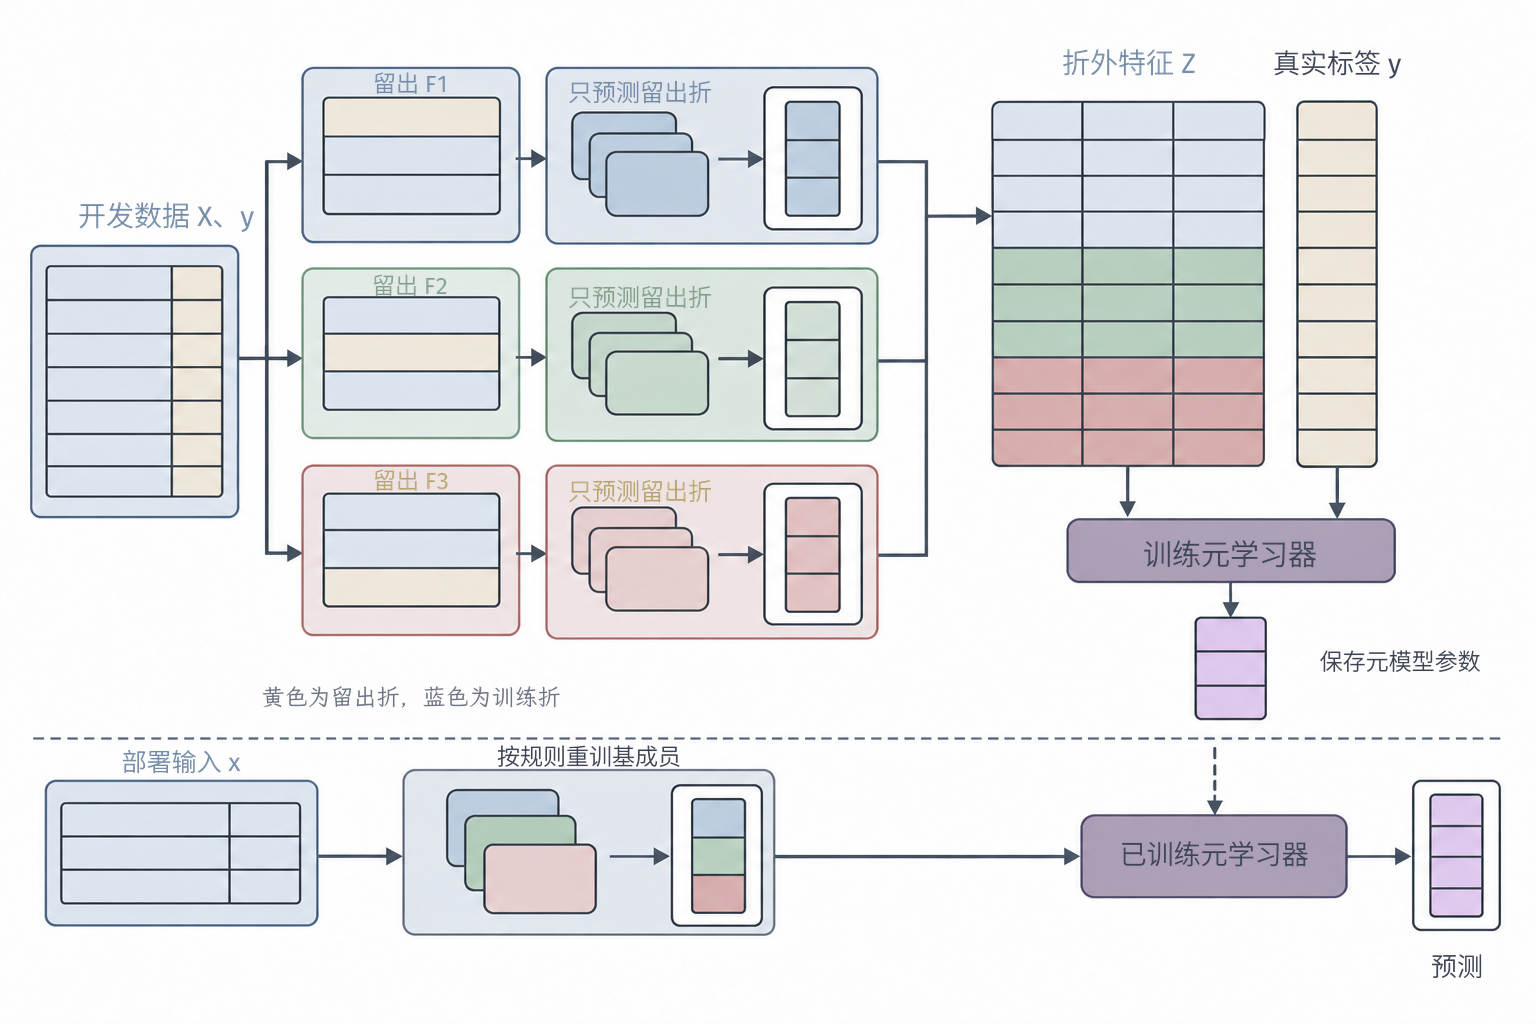
\includegraphics[width=130.048mm]{figures/03-models/01-classic-models/generated/ensemble-stacking-oof/figure.png}
  \caption{三折Stacking的折外特征构造。每一折轮流作为留出折，临时成员只在其余两折训练，并为留出折产生预测；拼接三次预测得到完整折外矩阵$\bm{Z}$，元学习器以$\bm{Z}$为输入并使用对应标签拟合。部署阶段的基成员还需按预先规定的方式重训或保留。}
  \label{fig:ensemble-stacking-oof}
\end{figure*}

分类成员若输出$C$维概率向量，一个成员通常贡献$C$列元特征；二分类时也可以只保留一个类别概率。类别硬判断省去了得分中的排序或置信信息，不同成员的得分还可能采用不同尺度。元训练与部署使用一致的输出形式，正则化再控制尺度及相关预测对组合的影响。

\subsubsection{部署模型与全量训练集重训}

折外矩阵用于训练元学习器，但部署时还需要能预测新输入的基成员。一种做法是在完整训练集上重新拟合每类基学习器$\widehat{h}_m$，预测
\[
  \widehat{y}
  =
  g\!\left(
    \widehat{h}_1(\bm{x}),\ldots,\widehat{h}_M(\bm{x})
  \right).
\]
全量重训利用全部开发数据，但训练规模增加可能改变预测分布，元学习器训练时只看过较小训练集产生的输出。也可保留各折成员，先平均它们对新输入的预测，再送入元学习器；这样沿用折内模型，同时增加了存储与推理次数。两方案的输入分布差异仍由完整验证检验。

部署方案确定后，需要评价基成员与元学习器共同形成的预测流程。基学习器的特征处理、类别编码和超参数搜索必须在相应训练折内完成。若先用全部数据选择特征或编码，再只把模型拟合放进交叉验证，信息仍可能从留出折进入元特征。

\subsection{Blending}
\label{sec:ensemble-blending}

\term{Blending}通过一次留出构造元特征，减少交叉验证的重复拟合。将可用于开发的数据分为基训练集$D_{\mathrm{base}}$和组合训练集$D_{\mathrm{blend}}$；基成员只在$D_{\mathrm{base}}$上拟合，对$D_{\mathrm{blend}}$产生预测，元学习器再以这些预测和对应标签训练。每个基成员只需完成一次用于元特征的拟合，流程比完整Stacking短。

训练数据由两层分用：基成员在$D_{\mathrm{base}}$拟合，元学习器只使用$D_{\mathrm{blend}}$的预测与标签。划分较小时，元学习器估计不稳定；划分较大时，基成员训练信息减少。多次随机划分并平均可以减小单次划分的偶然性，但它重新引入多次训练，已经不再具有单次Blending的全部成本优势。

部署时若把$D_{\mathrm{blend}}$加入基成员重新训练，基预测分布可能相对元学习器训练时发生变化；若不加入，则没有充分利用已有标签。重训方式因此属于模型配置，需要先确定，再用未参与选择的数据评价实际组合。

\subsection{受约束线性Stacking}
\label{sec:ensemble-constrained-linear-stacking}

若希望以较少参数学习成员贡献，可以在回归折外矩阵$\bm{Z}\in\mathbb{R}^{n\times M}$上学习线性组合
\begin{equation}
  (\widehat{b},\widehat{\bm{w}})
  \in
  \argmin_{b,\bm{w}}
  \frac{1}{n}
  \sum_{i=1}^{n}
  \ell\!\left(
    y_i,
    b+\bm{w}^{\top}\bm{z}_i
  \right)
  +\lambda\lVert\bm{w}\rVert_2^2.
  \label{eq:ensemble-linear-stacking}
\end{equation}
权重约束控制组合允许的尺度和方向。在$b=0$时，仅要求$w_m\geq0$得到非负线性组合，仍可能放大预测；仅要求$\sum_mw_m=1$得到仿射组合，仍可因负权重而外推。只有同时满足$b=0$、$w_m\geq0$和$\sum_mw_m=1$，才是成员预测的凸组合，输出必定位于成员预测的凸包内。非负约束排除了成员之间的正负抵消，归一化进一步限制整体尺度；有效校正若需要负权重或截距，约束会缩小候选类并增加逼近误差。

权重大小同时受输出尺度、成员相关性和损失函数影响。两个成员预测近乎相同，线性模型可以在它们之间任意分配相近作用；一个成员输出的数值范围更大，也会改变未标准化正则项下的权重。估计权重反映给定尺度、相关性与损失下的联合拟合，而非成员独立贡献。对同一类别集合上的概率向量，使用同一组满足上述凸组合条件的权重逐类组合，结果保持概率单纯形约束，样本外校准再检查概率与实际频率的对应。

\subsection{Super Learner}
\label{sec:ensemble-super-learner}

\term{Super Learner}把候选学习器库、交叉验证风险与组合权重放进一个明确程序。给定预先规定的候选库和损失，先生成每个候选的折外预测，再在指定组合类中选择交叉验证风险较小的组合；组合类可以是最佳单成员、非负线性组合或其他受控元模型。

在独立同分布、损失有界或满足相应矩条件、候选库与交叉验证方案受控等条件下，Super Learner的理论结果把其风险与候选组合类中的oracle风险联系起来：样本量增加时，交叉验证选择的组合能够渐近接近该库中最优候选或最优组合的风险\scite{vanderlaan2007superlearner}。oracle在预先给定的候选库、组合类和损失中取最优，其范围由这些设计确定。

这一比较依赖三类信息：候选库能提供什么预测，折外损失能多准确地估计目标风险，以及元模型复杂度是否得到样本支持。渐近接近oracle与有限样本中的实际改进需分别检查。若数据存在时间、群组或空间依赖，交叉验证划分还必须与部署时的新样本定义一致。

\subsection{模型对比与总结}
\label{sec:ensemble-stacking-comparison}

表\ref{tab:ensemble-stacking-comparison}比较Stacking家族的元特征来源与组合约束。标准Stacking和Super Learner都依赖折外预测；Blending以一次留出降低训练次数；受约束线性Stacking通过限制权重控制组合层容量。模型名称之外，还应记录预处理、基模型重训和元输出类型，否则无法复现实际预测链路。

\begin{table*}[htbp]
  \centering
  \small
  \begin{tabularx}{\linewidth}{@{}>{\raggedright\arraybackslash}p{25mm}*{5}{>{\raggedright\arraybackslash}X}@{}}
    \toprule
    方法 & 元特征来源 & 数据利用 & 组合规则 & 主要成本 & 主要风险 \\
    \midrule
    Stacking & $K$折折外预测 & 每个样本都产生元特征 & 可线性或非线性 & 每类成员需多次折内拟合 & 折外流程不完整造成泄漏 \\
    Blending & 固定留出集预测 & 元学习器只用留出集 & 可线性或非线性 & 基成员用于元特征时只拟合一次 & 划分敏感与重训分布变化 \\
    受约束线性Stacking & 通常为折外预测 & 与所用划分一致 & 非负、和为一或正则化线性组合 & 组合层较轻量 & 约束可能排除有效校正 \\
    Super Learner & 交叉验证预测与风险 & 由交叉验证方案决定 & 在预定库和组合类中选择 & 候选库越大，训练与选择成本越高 & oracle范围和有限样本被夸大 \\
    \bottomrule
  \end{tabularx}
  \caption{Stacking及其代表性变体。表中“数据利用”描述元学习器训练阶段；部署前是否用完整开发数据重训基成员，还需作为流程的一部分单独规定。}
  \label{tab:ensemble-stacking-comparison}
\end{table*}

多层Stacking把一层折外输出继续交给下一层，每增加一层都要重新保证当前样本没有通过上游拟合泄漏到本层特征。输入相关的门控组合则让权重随$\bm{x}$变化，它与第\ref{sec:ensemble-dynamic-selection}节的动态成员选择相邻，也与神经网络中的混合专家相接。它们增加了表达能力，同时扩大了数据划分、模型存储和调试成本；增加层数需要在相同数据与预算下取得新增预测收益，才能支持相应成本。

\section{成员选择与集成简化}
\label{sec:ensemble-selection-compression}

Bagging、Boosting和Stacking先回答怎样形成组合。部署时，多成员推理可能超出内存或延迟预算，一些成员也可能只在局部输入上有用。简化集成有三种不同目标：为所有输入固定一个较小成员子集，针对当前输入临时选择成员，或训练一个新的紧凑模型替代原集成。前两种方法保留部分原成员，第三种方法改变了部署模型。

图\ref{fig:ensemble-selection-compression}沿部署对象区分这三种目标。静态选择把成员池缩成一个固定子集，动态选择保留成员池并让路由依赖当前输入，紧凑化则把完整集成的行为转移到新模型。资源评价据此包括被部署模型以及选择或路由计算。

\begin{figure*}[htbp]
  \centering
  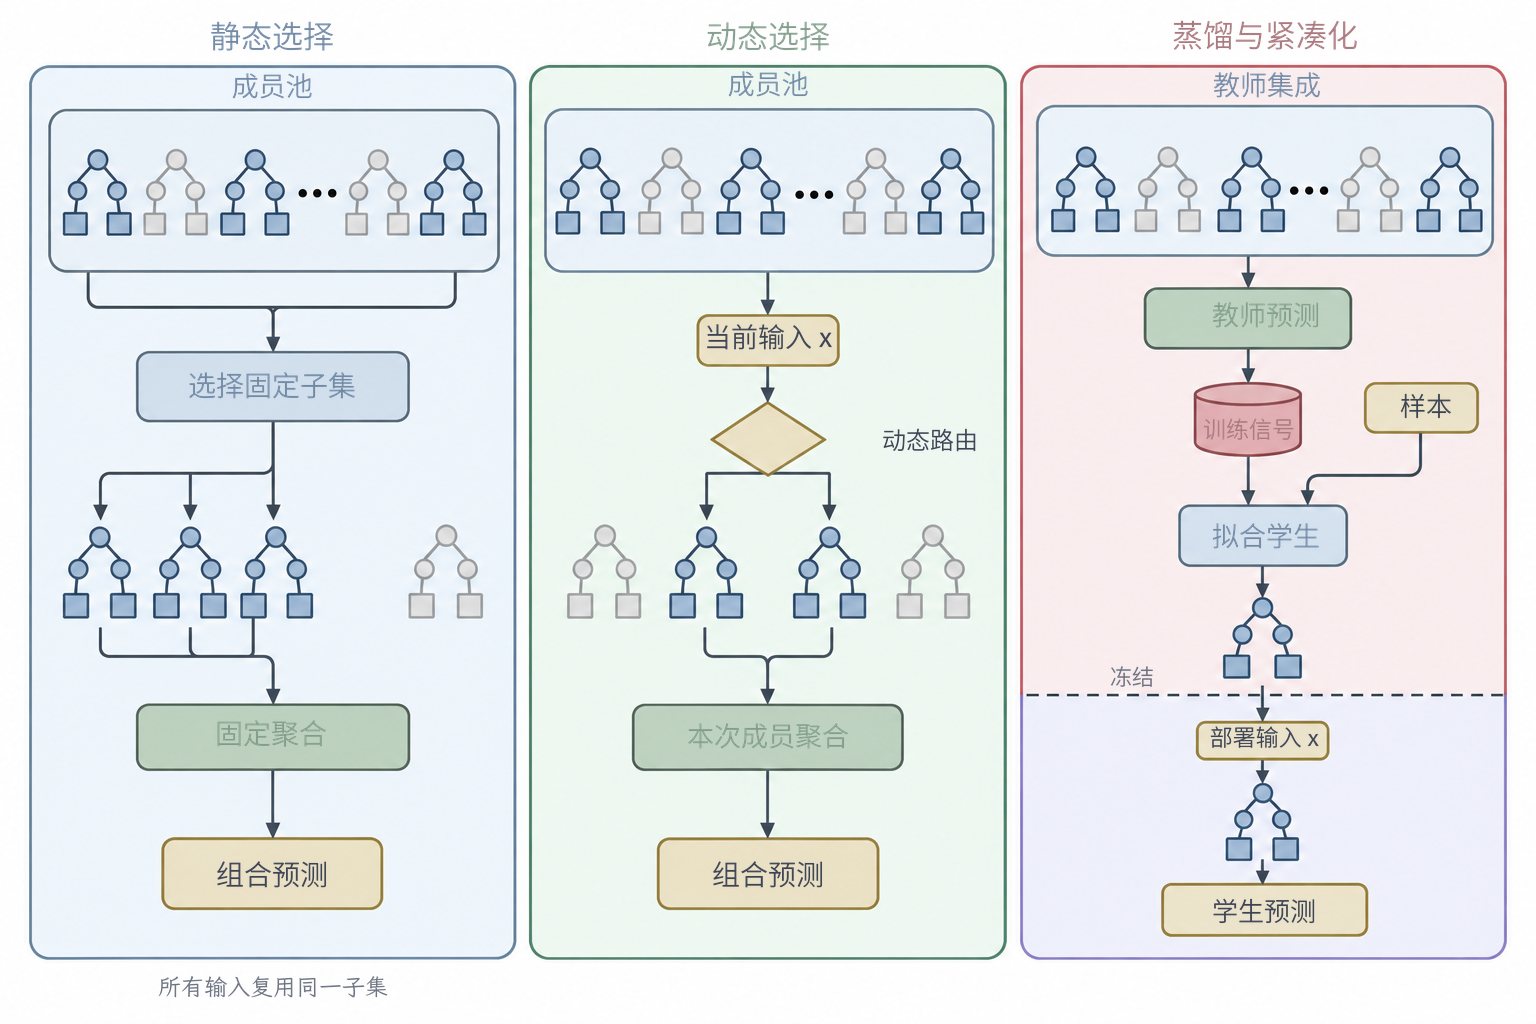
\includegraphics[width=130.048mm]{figures/03-models/01-classic-models/generated/ensemble-selection-compression/figure.png}
  \caption{静态成员选择、动态成员选择与紧凑化改变的部署对象。静态选择为所有输入保留同一成员子集；动态选择根据输入改变运行成员或组合权重；紧凑化训练并部署新的学生模型。三种路径改变的计算对象不同，成本需沿各自完整路径测量。}
  \label{fig:ensemble-selection-compression}
\end{figure*}

\subsection{静态成员选择}
\label{sec:ensemble-static-selection}

\term{静态成员选择}（static ensemble selection）给定已经训练好的候选池$\{h_1,\ldots,h_M\}$，选择一个对所有未来输入都相同的子集$S\subseteq\{1,\ldots,M\}$。若$\mathcal{L}_{\mathrm{val}}(S)$表示该子集按指定规则组合后的验证损失，可以写成
\begin{equation}
  \widehat{S}
  \in
  \argmin_{S\subseteq\{1,\ldots,M\}}
  \mathcal{L}_{\mathrm{val}}(S)
  +\lambda_1|S|
  +\lambda_2 C(S),
  \label{eq:ensemble-static-selection}
\end{equation}
其中$\lambda_1,\lambda_2\geq0$，$|S|$控制成员数，$C(S)$可以表示存储、单样本延迟或其他部署成本。成员池包含指数多个子集，实际可用排序、逐个加入或删除等方法近似搜索，并记录所得子集的验证损失与资源成本。

单成员排序忽略预测的重叠，可能同时保留许多相似模型。前向选择则评价候选加入当前组合后的损失变化，使选择依赖已有成员。允许重复选择某个成员时，重复次数还形成离散权重。基于模型库的贪心集成选择就是这种做法的代表：从一个初始组合出发，每轮加入使验证指标改善最大的候选，必要时使用多起点或装袋法减少搜索的不稳定性\scite{caruana2004ensemble}。

式\eqref{eq:ensemble-static-selection}的搜索对象为固定池中的成员子集，成员预测已经形成。若同时改变基学习算法、特征处理和超参数，搜索范围已经扩展为完整模型开发流程。候选池越大，验证集上偶然出现有利组合的机会也越多；最终测试需在该子集及其组合规则固定后进行。

分歧和误差协方差可以诊断预测关系，组合选择则以任务损失为直接依据。一个与其他成员高度不同但经常出错的模型，可能增加分歧而降低组合质量。静态选择应直接评价选定组合的输出，并在相同成员数或资源预算下与完整集成及单模型基线比较。

\subsection{动态成员选择}
\label{sec:ensemble-dynamic-selection}

静态方案让所有输入使用相同子集；若成员能力随输入区域改变，可将邻近记录上的预测结果用于当前选择。\term{动态分类器选择}（dynamic classifier selection, DCS）为每个输入选择一个成员；\term{动态集成选择}（dynamic ensemble selection, DES）选择一个成员子集或给出输入相关权重。

一种基本构造是准备独立的能力估计数据。对查询输入$\bm{x}$，在该数据中寻找非空邻域$\mathcal{N}(\bm{x})$，再以成员$m$在邻域内的正确率估计
\begin{equation}
  \widehat{c}_m(\bm{x})
  =
  \frac{1}{|\mathcal{N}(\bm{x})|}
  \sum_{i\in\mathcal{N}(\bm{x})}
  \mathbb{I}\!\left\{h_m(\bm{x}_i)=y_i\right\}.
  \label{eq:ensemble-local-competence}
\end{equation}
DCS可以选择$\widehat{c}_m(\bm{x})$最大的成员，DES则保留超过阈值的成员或按能力加权。局部正确率只是能力估计的一种方式，还可以使用输出轮廓、分类间隔或由元模型学习的能力特征\scite{woods1997localaccuracy}。

局部选择依赖邻域和能力估计两部分。邻域依赖输入表示与距离，高维或分布稀疏时，附近样本未必提供稳定的局部证据；能力估计器也可能在有限数据上过拟合。成员训练数据、能力估计数据与最终测试数据需要分开，所有标准化和邻域参数都在相应开发流程内确定。

动态选择的延迟由路由和实际运行成员共同决定。若系统必须先运行全部成员才能构造输出轮廓，再选择其中几个聚合，选择之前已经支付全部成员计算；基于输入邻域的方法还增加了检索成本。在昂贵成员运行前完成路由，才可能直接省去被跳过成员的计算；局部检索、路由和输出质量需要一并测量。

\subsection{从集成模型到紧凑模型}
\label{sec:ensemble-compression}

若原成员的最小可用子集仍超预算，可以另外训练一个新的\term{紧凑模型}（compact model），使其逼近完整集成的输入输出映射。早期模型压缩工作已经用大型集成的输出训练较小模型；知识蒸馏随后把这种教师到学生的传递扩展为常用训练形式\scite{bucilua2006compression,hinton2015distilling}。

设完整集成为教师$H$，紧凑模型为学生$s_{\bm{\theta}}$。对回归，可以组合真实响应损失与教师拟合损失：
\begin{equation}
  \min_{\bm{\theta}}
  \sum_{i=1}^{n}
  \left[
    \alpha\ell\!\left(y_i,s_{\bm{\theta}}(\bm{x}_i)\right)
    +(1-\alpha)
    \ell\!\left(H(\bm{x}_i),s_{\bm{\theta}}(\bm{x}_i)\right)
  \right],
  \label{eq:ensemble-compression-objective}
\end{equation}
其中$\alpha\in[0,1]$控制真实标签与教师输出的作用。分类时可以拟合教师的完整类别分布；温度缩放会使非最大类别之间的相对关系更容易进入训练信号，但温度、损失权重与部署概率仍须分别选择和校准。

学生训练输入可以来自原训练集、额外未标注样本或经过说明的合成样本。教师在所选输入上提供训练目标；覆盖不足的区域缺少这种监督，学生在这些区域仍可能偏离教师。学生容量过小会产生逼近误差，容量很大则可能无法达到预期资源节省。

紧凑化同时改变预测器与资源开销，可从四方面评价。预测一致性衡量学生是否复现教师输出；任务性能检查学生面对真实标签的风险；概率评价检查蒸馏后的得分是否仍可解释；资源测量确认模型大小、内存和延迟是否实际下降。训练输入上的一致性只描述局部逼近，新样本任务损失另外检查未来预测。真实标签、正则或额外数据也可使学生在部分区域改进教师预测。学生采用不同模型和训练过程，其解释、诊断及理论条件需按新模型建立。

\section{模型选择与评价}
\label{sec:ensemble-evaluation}

\subsection{成员质量、错误依赖与多样性}
\label{sec:ensemble-quality-dependence-diversity}

平均的作用可通过预测方差分析。固定输入$\bm{x}$，将训练集抽样、重采样与训练过程的随机性纳入概率空间。若$M$个成员预测具有相同方差$\sigma^2(\bm{x})$，任意两个不同成员的预测相关系数均为$\rho(\bm{x})$，则等权平均的方差为
\begin{equation}
  \operatorname{Var}\!\left[H(\bm{x})\right]
  =
  \sigma^2(\bm{x})
  \left[
    \rho(\bm{x})
    +
    \frac{1-\rho(\bm{x})}{M}
  \right].
  \label{eq:ensemble-correlated-variance}
\end{equation}
有限$M>1$时，协方差矩阵的半正定性要求$\rho(\bm{x})\geq-1/(M-1)$，因此允许一定负相关。在非负相关且增加成员时保持这一相关结构的设定下，随$M$衰减的项可解释为成员不共享的波动，$\rho(\bm{x})\sigma^2(\bm{x})$则是继续平均后保留的共同部分。式\eqref{eq:ensemble-correlated-variance}依赖等方差、等相关的简化设定，说明成员依赖对预测方差的作用；任务风险还需要结合偏差、响应噪声及相应损失。

图\ref{fig:ensemble-error-dependence}把这一差别写成成员误差的两部分。成员特有波动$u_m$在平均中可能相互抵消；若每个成员都带有共同误差$c$，增加同类成员只能继续削弱前一部分，不能消除$c$。树数控制平均次数，误差依赖控制共同部分，两者分别影响组合。

\begin{figure*}[htbp]
  \centering
  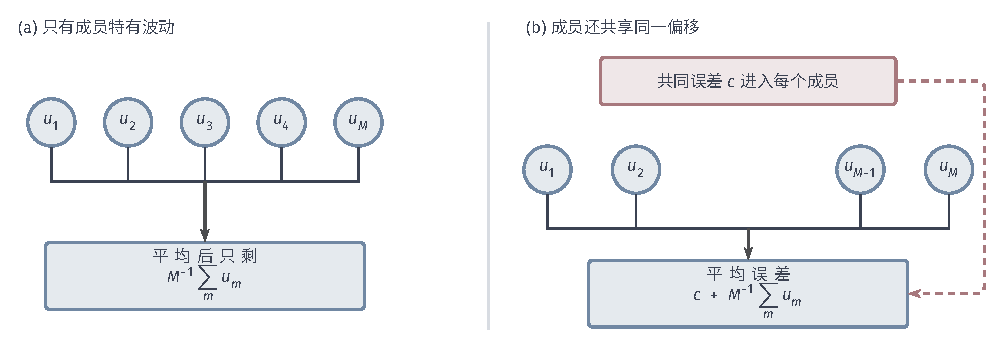
\includegraphics[width=169.000mm]{figures/03-models/01-classic-models/tikz/ensemble-error-dependence/figure.pdf}
  \caption{成员误差依赖与平均的作用。左图表示只有成员特有波动时，平均可以随成员数增加而削弱这些波动；右图表示所有成员还共享误差$c$时，共同项仍保留在平均预测中。图中成员数量与符号只用于说明机制，不表示实测误差。}
  \label{fig:ensemble-error-dependence}
\end{figure*}

平方误差还给出另一个逐点恒等式。对非负权重$w_m$且$\sum_mw_m=1$，令$H(\bm{x})=\sum_mw_mh_m(\bm{x})$，则
\begin{equation}
  \bigl(y-H(\bm{x})\bigr)^2
  =
  \sum_{m=1}^{M}w_m\bigl(y-h_m(\bm{x})\bigr)^2
  -
  \sum_{m=1}^{M}w_m\bigl(h_m(\bm{x})-H(\bm{x})\bigr)^2.
  \label{eq:ensemble-ambiguity-decomposition}
\end{equation}
右侧第一项是成员平方误差的加权平均，第二项衡量成员围绕组合预测的分散程度，常称为歧义项\scite{krogh1995ensembles}。在成员平均误差固定时，更大的有效分散会降低组合误差；但若为了制造分散而加入很差的成员，第一项也会增大。组合的平方误差由加权成员误差与歧义项共同决定。

分类投票直接依赖各成员在哪些样本上出错。除单成员错误率外，还需记录它们的共同错误。对一对分类器，可以记录二者同时正确、只有一个正确和同时错误的样本数$n_{1,1},n_{1,0},n_{0,1},n_{0,0}$。正确性分歧率$(n_{1,0}+n_{0,1})/n$描述二者给出不同正确性结果的频率。二分类时，它等于标签分歧率；多分类时，两者同时错误也可能给出不同标签。双错率$n_{0,0}/n$直接关注共同错误；Q统计量
\[
  Q=
  \frac{n_{1,1}n_{0,0}-n_{1,0}n_{0,1}}
       {n_{1,1}n_{0,0}+n_{1,0}n_{0,1}}
\]
在分母非零时描述两种正确性结果的关联。不同指标分别描述分歧、共同错误或正确性的关联；评价集成风险时，还需结合成员准确率、组合规则与任务损失\scite{kuncheva2003diversity}。

成员差异可以从多个位置产生。改变训练样本会改变成员看到的经验分布；改变输入特征会改变可用信息；改变模型结构或超参数会改变表示与正则；改变初始化、样本顺序或分裂候选会改变优化路径。Bagging主要扰动训练样本，随机森林和Extra Trees进一步扰动特征或阈值，Stacking则允许直接组合不同模型族。这些扰动产生预测差异，差异能否减少任务错误由样本外组合损失检验。

从表达能力看，成员函数族与组合类共同规定候选预测。固定平均保留成员共有的逼近限制，加法模型逐步扩展函数，元学习器则学习成员输出之间的关系。输入相关权重还能改变不同区域的组合。

从收敛性看，Bagging增加成员数是在固定数据上逼近随机预测的平均；Boosting搜索增量并控制所选训练目标；Stacking另需求解元模型。随机平均稳定、经验目标下降及找到候选类全局最优属于不同结论，各自采用对应抽样或优化条件。

从泛化性看，成员质量、共同错误与组合复杂度都影响新样本风险。上面的方差和平方误差关系说明误差依赖的作用，独立评价再检查实际预测。折外构造、成员筛选和验证选择形成的数据依赖，也需纳入最终流程。


\subsection{方法比较}
\label{sec:ensemble-method-comparison}

表\ref{tab:ensemble-method-navigation}按成员来源、依赖和组合规则比较本章方法。相同成员数可能对应不同的模型容量与成本：Bagging的一棵深树负责完整预测，Boosting的一棵浅树只提供增量，Stacking的一个成员甚至可能是已经包含许多树的随机森林。容量与成本必须沿完整训练和预测路径衡量。

\begin{table*}[htbp]
  \centering
  \small
  \begin{tabularx}{\linewidth}{@{}>{\raggedright\arraybackslash}p{23mm}*{6}{>{\raggedright\arraybackslash}X}@{}}
    \toprule
    方法 & 成员来源 & 成员间依赖 & 组合规则 & 训练并行性 & 推理路径 & 主要失效来源 \\
    \midrule
    Bagging & 重采样或随机权重下的同类成员 & 给定原训练集后可独立生成 & 平均、投票或固定加权 & 成员间可并行 & 通常运行全部成员 & 成员稳定或共同偏差占主导 \\
    随机森林／Extra Trees & 样本、特征与阈值的随机树 & 树之间无序贯依赖 & 平均或投票 & 树间可并行 & 运行全部或选定树 & 随机化削弱单树，或相关性仍高 \\
    AdaBoost & 当前样本权重下的弱分类器 & 第$t$轮依赖前轮权重 & 训练中确定的加权投票 & 轮次串行 & 累加全部或截断成员 & 噪声记录持续获得大权重 \\
    梯度提升树 & 当前损失梯度下的回归树 & 第$t$轮依赖$F_{t-1}$ & 收缩后的加法得分 & 轮次串行，单轮可并行 & 顺序累加树输出 & 损失、轮数、树复杂度与采样失配 \\
    Stacking & 同质或异质候选模型 & 基成员可独立，元层依赖折外预测 & 学习得到的元模型 & 折与成员可部分并行 & 运行基成员后再运行元模型 & 元特征泄漏、成员冗余或元层过拟合 \\
    动态选择／紧凑化 & 已训练成员池或教师集成 & 依赖能力估计或教师输出 & 输入相关选择或新学生模型 & 依具体训练流程而定 & 选择部分成员，或只运行学生 & 路由失准、覆盖不足或逼近误差 \\
    \bottomrule
  \end{tabularx}
  \caption{集成方法的属性导航。表中成本描述方法结构，不构成固定速度排序；实际结果还受成员模型、实现、硬件、数据规模与调参预算影响。}
  \label{tab:ensemble-method-navigation}
\end{table*}

方法比较还要固定组合输出。回归均值、分位数和分布各有评价损失，分类标签、排序和概率也有不同指标。准确率的变化描述标签预测，概率校准与尾部代价则另用对应证据评价。具体指标沿用表\ref{tab:regression-evaluation-protocol}和表\ref{tab:classification-evaluation-protocol}，本节补充集成特有的数据隔离与资源记录。

\subsection{数据隔离与泄漏控制}
\label{sec:ensemble-data-isolation}

集成开发中，同一记录可能处于不同步骤的留出部分。按预测的生成方式及用途，可区分以下五类：
\begin{itemize}
  \item \term{袋外预测}来自未抽中当前样本的自助成员，用于Bagging内部诊断、置换重要性或相关构造。
  \item \term{折外预测}来自未使用当前折拟合的模型，用于训练Stacking元学习器，或为其他二阶段模型提供样本外特征。
  \item \term{能力估计预测}来自动态选择的独立开发数据，用于判断某个成员在当前输入附近是否可靠。
  \item \term{验证预测}用于选择成员数、树复杂度、学习率、组合约束、阈值与早停轮数。
  \item \term{测试预测}只在所有训练、选择、校准和部署规则冻结后产生，用于评价最终流程。
\end{itemize}
图\ref{fig:ensemble-data-isolation}把五类预测放回各自的数据路径。前四类仍处在模型开发阶段，允许影响规定范围内的诊断、二阶段训练或选择；测试预测位于流程冻结之后，只负责评价最终链路。标明生成与使用路径，可以检查当前标签是否经过拟合、选择或校准返回预测。

\begin{figure*}[htbp]
  \centering
  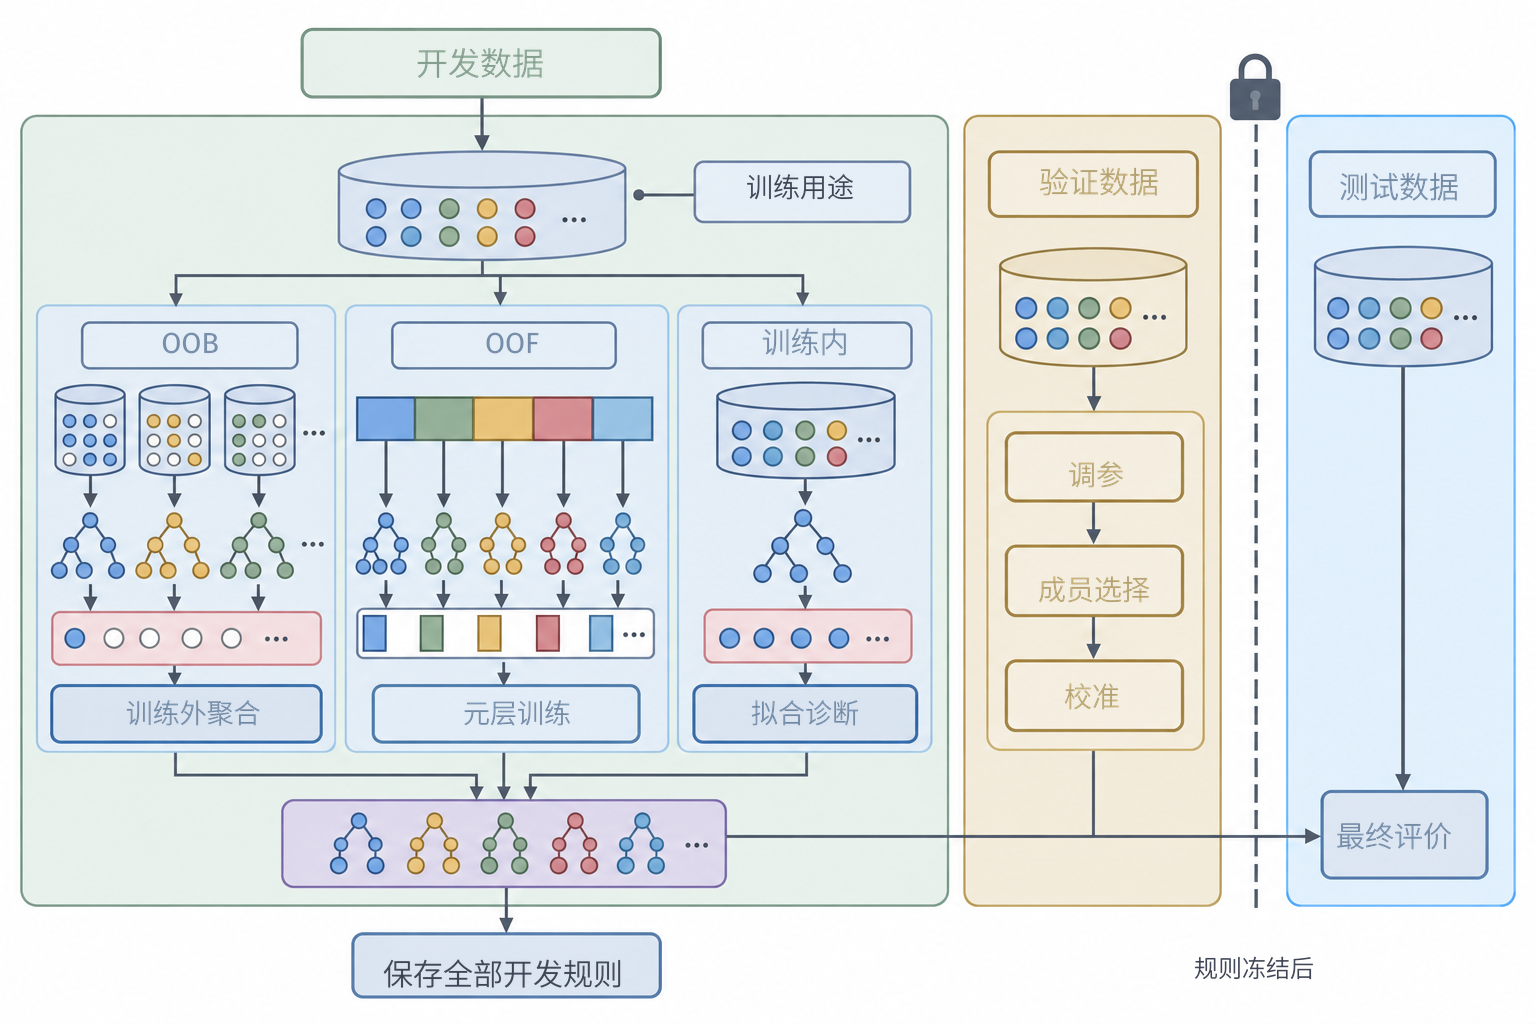
\includegraphics[width=130.048mm]{figures/03-models/01-classic-models/generated/ensemble-data-isolation/figure.png}
  \caption{集成学习中的数据隔离与预测职责。开发阶段的预测及验证数据各有规定用途；测试阶段前的竖直分隔线表示训练、调参、筛选、校准和部署规则已经冻结。测试预测评价已经冻结的流程；图中不向开发步骤返回选择信号。}
  \label{fig:ensemble-data-isolation}
\end{figure*}

留出条件只针对产生当前预测的拟合步骤，其后用途仍会引入新的数据依赖。折外矩阵参与元学习器训练，因而不是最终测试证据；袋外误差若反复用于选择随机森林参数，也已经参与模型开发；动态能力数据若同时训练成员，会高估局部能力。

泄漏还可能发生在模型拟合之前。缺失值填补、标准化、特征选择、目标编码和降维若利用了当前留出折，就会把信息带入折外预测。基成员调参、成员池筛选、元学习器调参和概率校准也要放在正确的数据层级。需要同时比较候选成员和组合规则时，可以在外层保留最终测试集，在内层训练折中完成全部预处理、调参及折外特征构造；时间、患者、用户或设备等依赖单位则按部署边界分组划分。

样本有限时，可用嵌套交叉验证或交叉拟合复用开发记录；每个用于评价或构造元特征的预测仍须由相应留出路径产生。应记录每个预测由哪些样本训练的哪些模型产生，使元训练、选择与最终评价的角色可追溯。

\subsection{预测质量与资源成本}
\label{sec:ensemble-quality-resource}

集成结果至少要与三个基线比较：相同任务下的合理单模型、未简化的完整集成，以及满足同一资源限制的候选方法。合理单模型提供基本预测参照，完整集成检验简化损失，同预算方法检验资源取舍。成员与组合的同时记录还可解释收益来自哪一步。

对Bagging，可以同时报告代表性单成员损失、成员预测相关或双错率、集成损失以及损失随成员数的变化。对Boosting，应区分训练损失、验证轨迹和最终测试结果，并记录早停轮数。对Stacking，应比较各成员的折外表现、折外预测依赖、元模型的新增验证收益和全链路测试结果。多样性记录用于解释依赖，选型仍以任务损失及预算为依据。

输出为概率时，需要检查数值与真实频率的对应。平均可保留成员共同的过度自信，提升得分则先经适当链接转换为概率。若使用后处理校准，校准器只能接收未用于拟合该预测的数据，并要把它作为部署链路的一部分，在最终测试集上报告对数损失、Brier分数、可靠性及任务决策损失。

资源比较记录预处理、成员、组合与路由的完整计算。训练侧至少包括总计算量、墙钟时间、峰值内存、并行资源和调参次数；部署侧包括序列化模型大小、加载内存、单样本延迟、批量吞吐及预处理和路由开销。Bagging的成员训练可以并行，但推理通常运行多个成员；Boosting轮次串行，树内统计可并行；Stacking既要运行基成员，又要运行元模型。静态选择、动态选择和紧凑化是否真正节省资源，只能由端到端测量回答。

\subsection{从问题条件到候选方法}
\label{sec:ensemble-method-selection}

当单模型对训练样本、随机种子或局部分裂明显敏感，并且可以承担多个成员的存储与预测成本时，Bagging是直接候选。树成员反复依赖少数强特征时，可以进一步比较随机森林；若阈值搜索成本较高且可以接受更强的随机化，再比较Extra Trees。在固定任务上比较单树变化、成员共同错误及组合损失，可以确认这些随机化是否带来所需收益。

当任务损失能够提供有意义的逐轮修正，并且训练流程可以承担序贯依赖时，可以考虑Boosting。AdaBoost适合检查重加权分类的机制；一般损失与树成员则进入GBDT。三种树提升系统的代表机制给出不同候选条件：需要分别判断是否重视正则化二阶树目标与稀疏路径、直方图及大规模稀疏统计、或类别特征的有序统计，并在当前硬件和搜索预算下实测。

当候选模型已经产生互补的样本外预测，而且可以承担交叉验证与多模型部署成本时，Stacking提供学习式组合。固定留出只让部分样本参加元训练，折外构造可让全部开发样本产生元特征；成员高度相关时，线性约束可以限制元模型的自由度。Super Learner的理论比较范围由候选库、损失和组合类共同决定，有限样本表现再按冻结流程评价。

成员池超过部署预算时，再判断要保留什么对象。希望所有输入走同一条较短路径时采用静态成员选择；有可靠局部能力数据且路由开销可控时考虑动态选择；完整集成质量合格但任何成员子集都达不到预算时，可以训练紧凑模型。以上条件只负责缩小候选范围，最终选择据相同数据制度、调参预算与资源测量下的新样本证据确定。


\Needspace{18\baselineskip}
\section{本章小结}
\label{sec:ensemble-summary}

集成利用成员生成与组合规则改变预测误差。互补作用来自成员能够在部分输入上修正彼此的判断，共同遗漏的结构仍需改变表示或训练方式。Bagging通过样本、特征或分裂随机性构造可并行成员，再用平均或投票削弱一部分训练波动；Boosting让每轮成员依赖当前组合，沿选定损失逐步加入修正；Stacking使用折外预测训练元学习器，使组合规则本身也由数据决定。三类机制可以嵌套，但各自的数据依赖、计算路径和失效原因不同。

成员池形成后，还可以改变部署规模。静态成员选择为所有输入固定同一子集，动态成员选择针对当前输入估计局部能力，紧凑化则训练一个新模型逼近完整集成。选择保留原成员的部分计算，紧凑化则部署一个重新训练的预测器，因此其成本与误差来源需要分别评价。

最终评价针对成员训练、选择和部署规则全部固定后的预测流程。袋外预测服务于Bagging内部诊断，折外预测服务于Stacking的元特征构造，能力估计数据服务于动态选择；前述预测用于开发，最终测试再评价冻结后的完整流程。比较方法时还要固定调参预算，并同时报告任务损失、概率质量、模型大小和端到端延迟。后续神经网络模型部分将在这些共同原则上，进一步讨论由初始化、数据顺序与训练过程产生的神经网络集成。

\paragraph{扩展阅读}
Hastie等的教材从加法建模解释提升方法；Breiman的Bagging与随机森林论文说明重采样及特征随机化的作用。可选同一预测任务，比较成员误差中可被组合削弱的部分，并记录获得这一收益所需的训练与部署成本\scite{hastie2009,breiman1996bagging,breiman2001randomforests}。

